\documentclass[12pt,a4paper]{report}
\renewcommand{\baselinestretch}{1.5}
\usepackage{cite}
\usepackage{fontspec}
% \usepackage[T1]{fontenc}
% \usepackage{times,newtxmath,newtxtext}

% ini coba ganti format
\usepackage{chngcntr}
\counterwithout{figure}{chapter}
\counterwithout{table}{chapter}
% ini coba ganti format
\usepackage{pifont}
\usepackage{placeins}
\usepackage[utf8]{inputenc}
\usepackage{subcaption}
\usepackage{setspace}
\usepackage{multirow}
\usepackage{multicol}
\usepackage[tableposition=top]{caption}
\usepackage[table,xcdraw]{xcolor}
\usepackage{varwidth}
\usepackage{titlesec}
\usepackage{indentfirst}
\usepackage{enumitem}
\usepackage{overpic}
\usepackage{tikz}
\usepackage{pdflscape}
\usepackage{xurl}
\usepackage{multirow}
\usepackage{amssymb}
\usepackage{tabularx}
\usepackage[table,xcdraw]{xcolor}
\setlength{\tabcolsep}{1.505625pt}
\renewcommand{\arraystretch}{1.2}
\usepackage{listings}
\usepackage{xcolor}
\usepackage{soul} % Required for highlighting
\definecolor{Gainsboro}{RGB}{232,232,232}
\definecolor{Gainsboro3}{RGB}{248,248,248}
\definecolor{highlightbg}{RGB}{255, 255, 153} % Define the highlight color
\lstdefinelanguage{myLang}
{
  % list of keywords
  morekeywords=[4]{Feature, Scenario},
  morekeywords=[2]{Given, When, Then, And},
  morekeywords=[3]{url, path, param, params, method, request, status, response},
  keywordstyle=[4]\color{blue}, % style of comments
  keywordstyle=[2]\color{magenta}, % style of comments
  keywordstyle=[3]\color{brown}, % style of comments
  sensitive=false, % keywords are not case-sensitive
  morecomment=[l]{#}, % l is for line comment
  morecomment=[s]{/*}{*/}, % s is for start and end delimiter
  morestring=[b]", % defines that strings are enclosed in double quotes
  escapeinside={*@}{@*}, % Define the escape characters
  rulecolor=\color{black}, % Define the frame color
}

% Define Colors
% \usepackage{color}
\definecolor{eclipseBlue}{RGB}{42,0.0,255}
\definecolor{eclipseGreen}{RGB}{63,127,95}
\definecolor{eclipsePurple}{RGB}{127,0,85}
 
% Set Language
\lstset{
  language={myLang},
  basicstyle=\small\ttfamily, % Global Code Style
  captionpos=b, % Position of the Caption (t for top, b for bottom)
  extendedchars=true, % Allows 256 instead of 128 ASCII characters
  tabsize=2, % number of spaces indented when discovering a tab 
  columns=fixed, % make all characters equal width
  keepspaces=true, % does not ignore spaces to fit width, convert tabs to spaces
  showstringspaces=false, % lets spaces in strings appear as real spaces
  breaklines=true, % wrap lines if they don't fit
  frame=lines,
  numbers=left, % show line numbers at the left
  numberstyle=\tiny\ttfamily, % style of the line numbers
  commentstyle=\color{eclipseGreen}, % style of comments
  keywordstyle=\color{eclipsePurple}, % style of keywords
  stringstyle=\color{eclipseBlue} % style of strings
}

\setlength{\tabcolsep}{10pt} % Default value: 6pt
\renewcommand{\arraystretch}{1.5} % Default value: 1

\usepackage{longtable}
% % \usepackage[margin=2cm,landscape]{geometry}
% \usepackage[english]{babel}

\usepackage{array,ragged2e}
\newcolumntype{P}[1]{>{\justifying\arraybackslash}p{#1}}


\setlist{nosep}
\setlength{\parindent}{1cm}
\usepackage[font=small,labelfont=bf,labelsep=space]{caption}

\captionsetup[longtable]{labelsep=space}
\captionsetup[table]{labelsep=space}
\captionsetup[figure]{labelsep=space}
% \usepackage[font=small,labelfont=bf]{caption}
\usepackage[numbers]{natbib}

\usetikzlibrary{shapes.geometric, arrows}
\definecolor{blu}{RGB}{135,206,250}
\definecolor{ore}{RGB}{255,140,0}
\tikzstyle{process} = [rectangle, rounded corners, minimum width=4cm, minimum height=1cm, text centered, text width=5cm, draw=black, fill=blu]
\tikzstyle{process2} = [rectangle, rounded corners, minimum width=3cm, minimum height=1cm, text centered, text width=3cm, draw=black, fill=blu]
\tikzstyle{decision} = [diamond, minimum width=2.2cm, minimum height=0.3cm, text centered, text width=1.1cm, draw=black, fill=orange!40]
\tikzstyle{arrow} = [thick,->,>=stealth]

\usepackage{gensymb}
\usepackage{notoccite}
\usepackage{float}
\usepackage[colorlinks,
  citecolor=black,
  linkcolor=black,
  urlcolor=black]{hyperref}
  \urlstyle{rm}
\usepackage{indentfirst}
\usepackage{amsmath}
% \usepackage{breakurl}
\usepackage{listings}
% \usepackage{natbib}

%%%%%%%
\title{\huge \bfseries SKRIPSI}
\author{825230066 CELVIN}

\renewcommand{\chaptername}{BAB }
% \renewcommand{\figurename}{\textbf{Gambar}}
\renewcommand{\figurename}{}
% \renewcommand{\tablename}{Tabel}
\renewcommand{\tablename}{}
\renewcommand{\lstlistingname}{\textbf{Kode}}
\renewcommand{\contentsname}{DAFTAR ISI}
\renewcommand{\listtablename}{DAFTAR TABEL}
\renewcommand{\listfigurename}{DAFTAR GAMBAR}
\renewcommand{\lstlistlistingname}{DAFTAR KODE}
\renewcommand{\bibname}{DAFTAR PUSTAKA}

\renewcommand{\thechapter}{\Roman{chapter}}
\renewcommand{\thesection}{\arabic{chapter}.\arabic{section}.}
\renewcommand{\thesubsection}{\arabic{chapter}.\arabic{section}.\arabic{subsection}.}
\renewcommand{\thesubsubsection}{\arabic{chapter}.\arabic{section}.\arabic{subsection}.\arabic{subsubsection}.}


%ini test format juga ke dua
\renewcommand{\thefigure}{Gambar \arabic{figure}}
\renewcommand{\thetable}{Tabel \arabic{table}}
%ini test format juga ke dua

% \renewcommand{\thefigure}{\arabic{chapter}.\arabic{figure}}
% \renewcommand{\thetable}{\arabic{chapter}.\arabic{table}}
\renewcommand{\theequation}{\arabic{chapter}.\arabic{equation}}

\AtBeginDocument{
\renewcommand\thelstlisting{\arabic{chapter}.\arabic{lstlisting}}
}



\usepackage{graphicx}
\usepackage[a4paper,top=40mm,bottom=30mm,left=40mm,right=30mm]{geometry}

\usepackage{tocloft}
\renewcommand{\cftsecleader}{\cftdotfill{\cftdotsep}}
\renewcommand{\cftchapfont}{\bfseries}
\renewcommand{\cftchappagefont}{\bfseries}
\renewcommand{\cftchappresnum}{BAB }
\renewcommand{\cftchapaftersnum}{.}
\renewcommand{\cftchapnumwidth}{4em}
\renewcommand{\cfttoctitlefont}{\hspace*{\fill}\Large\bfseries}
\renewcommand{\cftaftertoctitle}{\hspace*{\fill}}
\renewcommand{\cftlottitlefont}{\hspace*{\fill}\Large\bfseries}
\renewcommand{\cftafterlottitle}{\hspace*{\fill}}
\renewcommand{\cftloftitlefont}{\hspace*{\fill}\Large\bfseries}
\renewcommand{\cftafterloftitle}{\hspace*{\fill}}

\usepackage{sectsty}
\usepackage{dirtree}

\newcounter{appendixletter}
\renewcommand{\theappendixletter}{\Roman{appendixletter}}

\newcommand{\nextappendix}{\stepcounter{appendixletter}}
\newcommand{\customappendixlabel}[1]{\label{#1}}


\chapternumberfont{\Large} 
\chaptertitlefont{\Large}
\pagenumbering{roman}
\sectionfont{\normalsize}
\subsectionfont{\normalsize}
\titleformat{\section}{\large\bfseries}{\thesection}{1em}{}
\titlespacing\section{0pt}{12pt plus 4pt minus 2pt}{0pt plus 2pt minus 2pt}
\titlespacing\subsection{0pt}{12pt plus 4pt minus 2pt}{0pt plus 2pt minus 2pt}
\titlespacing\subsubsection{0pt}{12pt plus 4pt minus 2pt}{0pt plus 2pt minus 2pt}

\titleformat{\chapter}[display]
	{\normalfont\large\bfseries\centering}{\chaptertitlename \thechapter \centering}{-10pt}{\large}
\titlespacing*{\chapter}{0pt}{-30pt}{20pt}

\setcounter{secnumdepth}{4}
\setcounter{tocdepth}{4}

\usepackage{xcolor}
% \definecolor{Gainsboro}{RGB}{220, 220, 220}
\definecolor{codegreen}{rgb}{0,0.6,0}
\definecolor{codegray}{rgb}{0.5,0.5,0.5}
\definecolor{codepurple}{rgb}{0.58,0,0.82}
\definecolor{backcolour}{rgb}{1,1,1}

\lstdefinestyle{mystyle}{
    backgroundcolor=\color{backcolour},   
    commentstyle=\color{codegreen},
    keywordstyle=\color{magenta},
    numberstyle=\tiny\color{codegray},
    stringstyle=\color{codepurple},
    basicstyle=\ttfamily\footnotesize,
    breakatwhitespace=false,         
    breaklines=true,                 
    captionpos=b,                    
    keepspaces=true,                 
    numbers=left,                    
    numbersep=5pt,                  
    showspaces=false,                
    showstringspaces=false,
    showtabs=false,                  
    tabsize=2
}

\lstset{style=mystyle}


\setmainfont{Calibri}[
    Path=./Font/,
    Extension = .ttf,
    UprightFont=*-regular,
    BoldFont=*-bold,
    ItalicFont=*-italic,
    BoldItalicFont=*-bold-italic
]

\begin{document}
% \newgeometry{a4paper,top=4cm,bottom=3cm,left=4cm,right=3cm}
\newgeometry{a4paper,top=2.5cm,bottom=3.5cm,left=2cm,right=2cm}

% \begin{titlepage}
\center 
\makeatletter

\includegraphics[width=5.8cm]{Gambar/logo-untar.png}\\[0.2cm]
\@title \\[2cm]
{\large Judul: \vspace{-2.3ex}
\\ \normalfont PERANCANGAN APLIKASI DATA \textit{ARCHIVING} OTOMATIS DAN PORTAL \textit{ON-DEMAND RETRIEVAL} BERBASIS WEB ASP.NET PADA PUSDATIN UNTAR}
\quad\\[2cm]
\begin{minipage}[t]{\textwidth}
\begin{center} \large
\textbf{Disusun oleh:}\\
\normalfont \@author 
\end{center}
\end{minipage}
\makeatother
\\[2cm]
\large PROGRAM STUDI SISTEM INFORMASI\\
\large FAKULTAS TEKNOLOGI INFORMASI\\
\large UNIVERSITAS TARUMANAGARA\\[0.2cm]
{\large  2026}
\end{titlepage}
\chapter*{\centering}
\thispagestyle{empty}
\addcontentsline{toc}{chapter}{JUDUL}
\begin{center}
    \vspace{-0.5cm}
    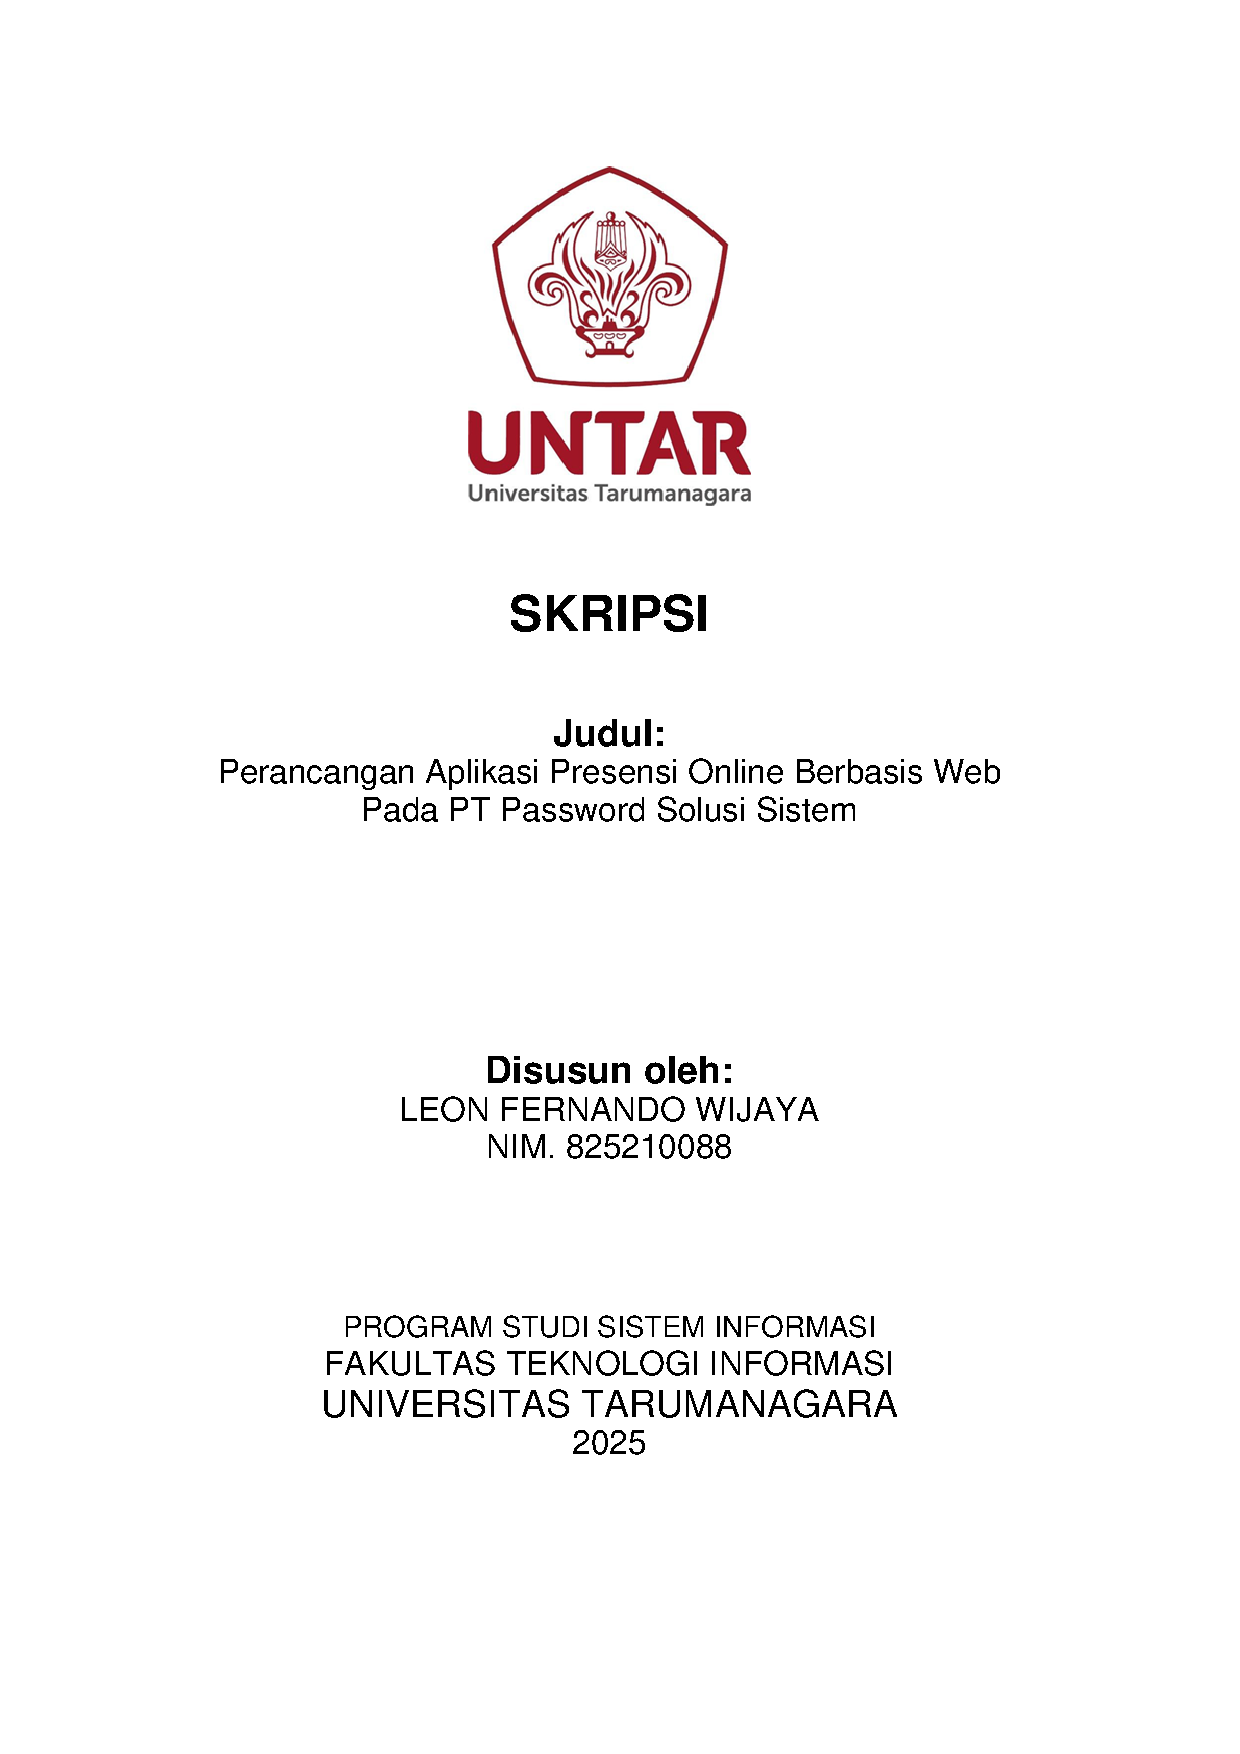
\includegraphics[page=1, scale=3, width=18cm, trim={0.75cm 2cm 0cm 2.8cm}, clip]{Header/cover-proposal.pdf}
\end{center}
    

\newpage
\input{Header/persetujuan-proposal-skripsi}
\chapter*{\centering }

\setstretch{1.5}
\thispagestyle{empty}

\addcontentsline{toc}{chapter}{LEMBAR PERSETUJUAN SKRIPSI}
\begin{center}
    % \vspace{0.75cm}
    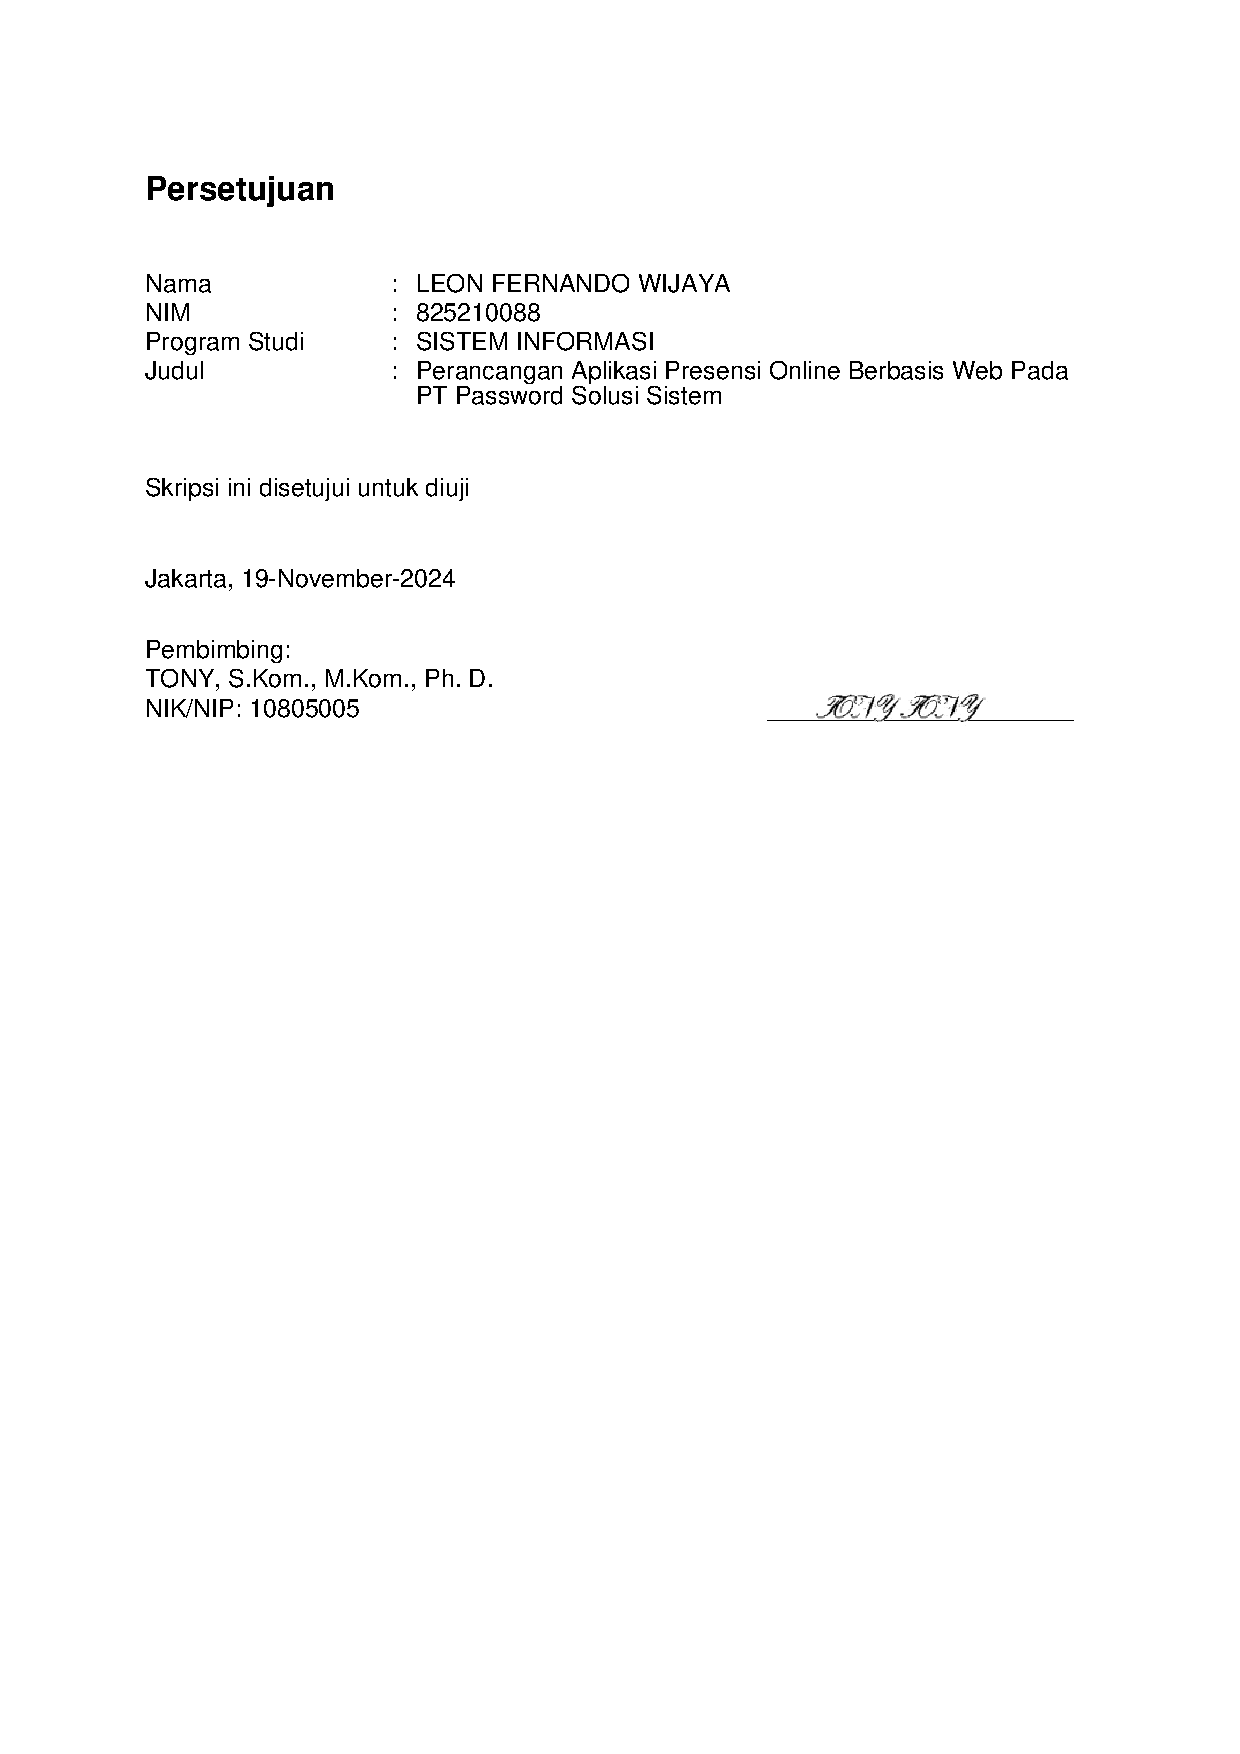
\includegraphics[page=1, scale=3, width=17cm, trim={2cm 7cm 2cm 2cm}, clip]{Header/persetujuan.pdf}
\end{center}

\chapter*{\centering }

\setstretch{1.5}
\thispagestyle{empty}

\addcontentsline{toc}{chapter}{LEMBAR PENGESAHAN}
% \begin{center}
%     % \vspace{0.75cm}
%     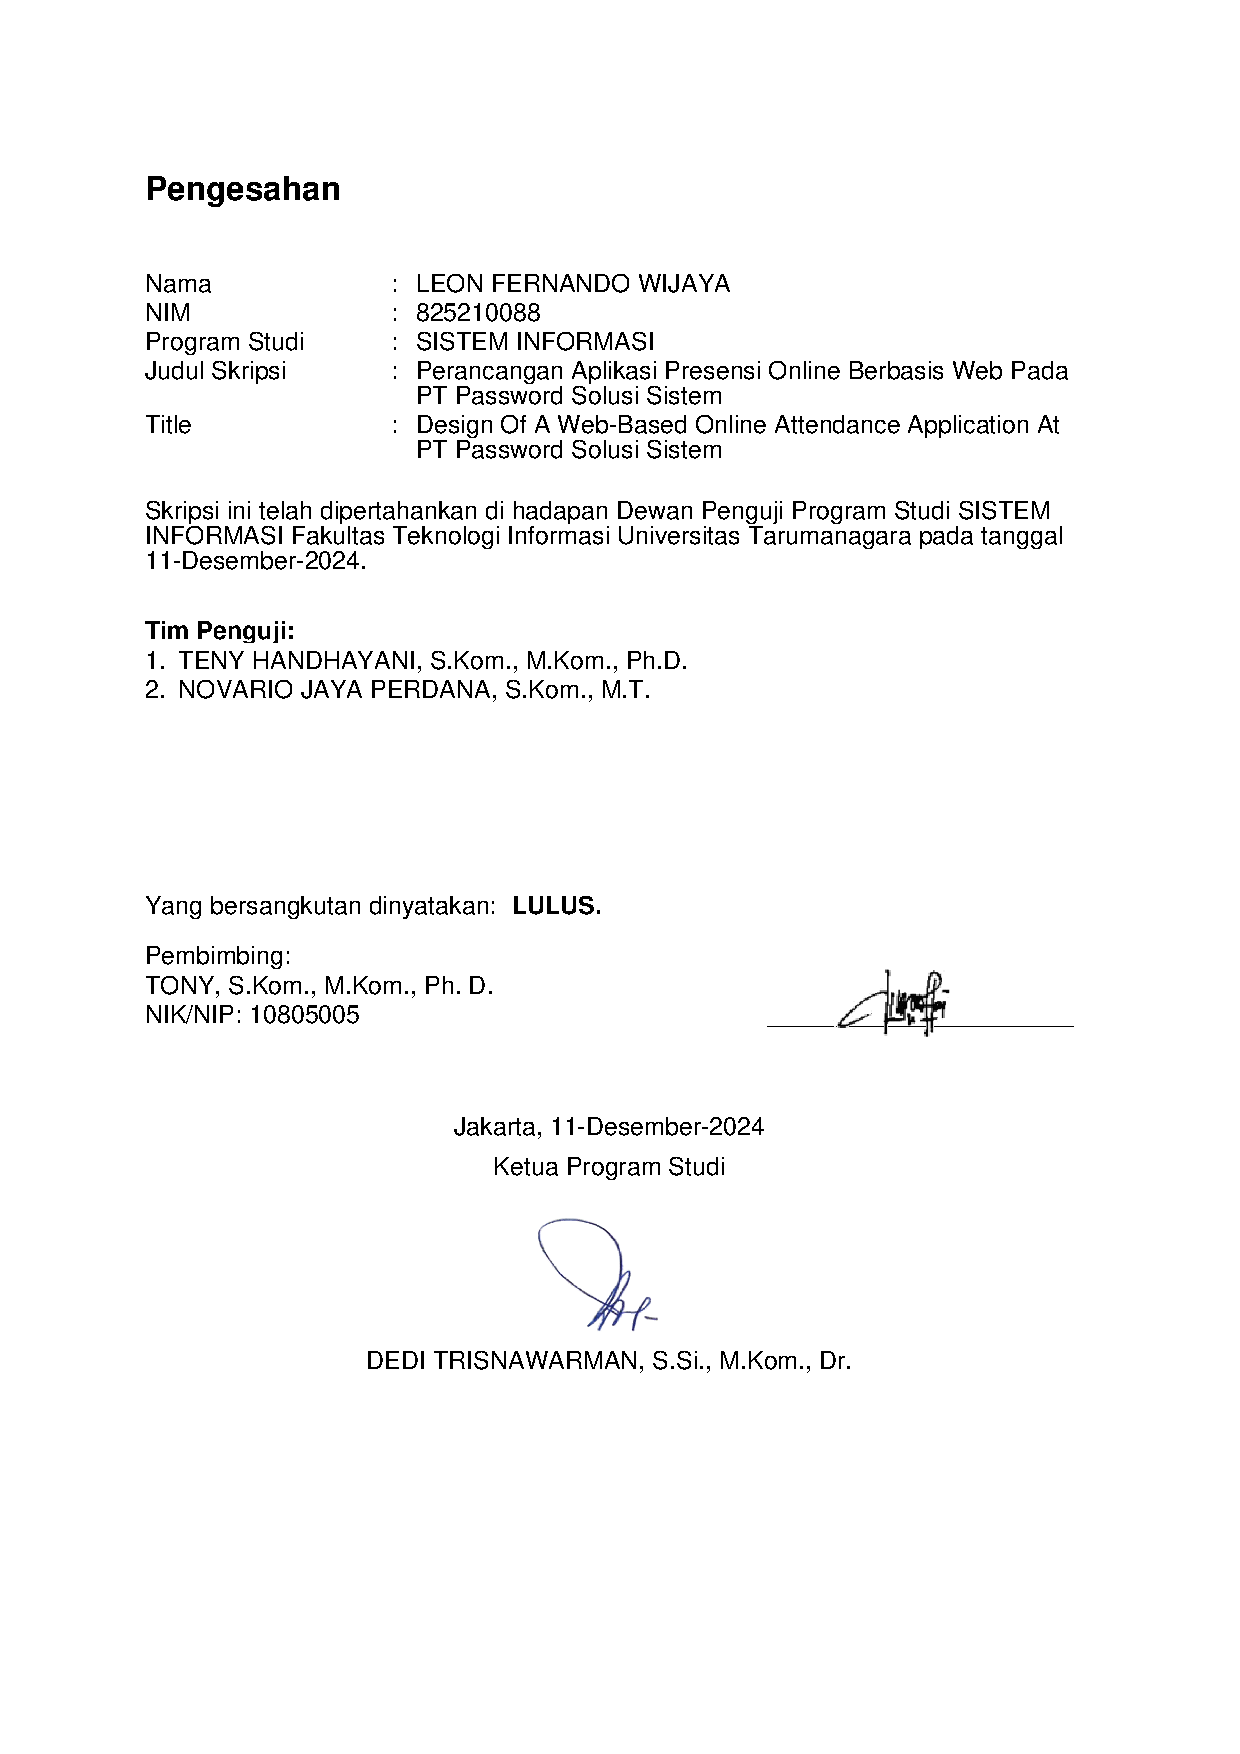
\includegraphics[page=1, scale=3, width=17cm, trim={0cm 2cm 0cm 2cm}, clip]{Header/pengesahan-skripsi.pdf}
\begin{center}
    % \vspace{0.75cm}
    \begin{figure}[!htbp]
	\centering
	% 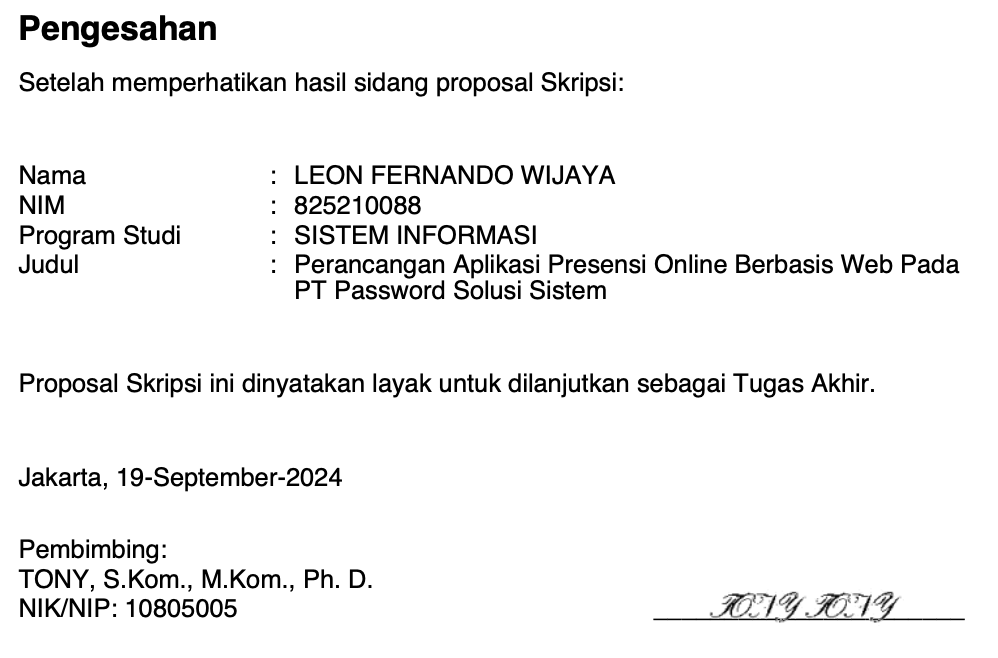
\includegraphics[width=0.9\textwidth]{Header/pengesahan-proposal.png}
        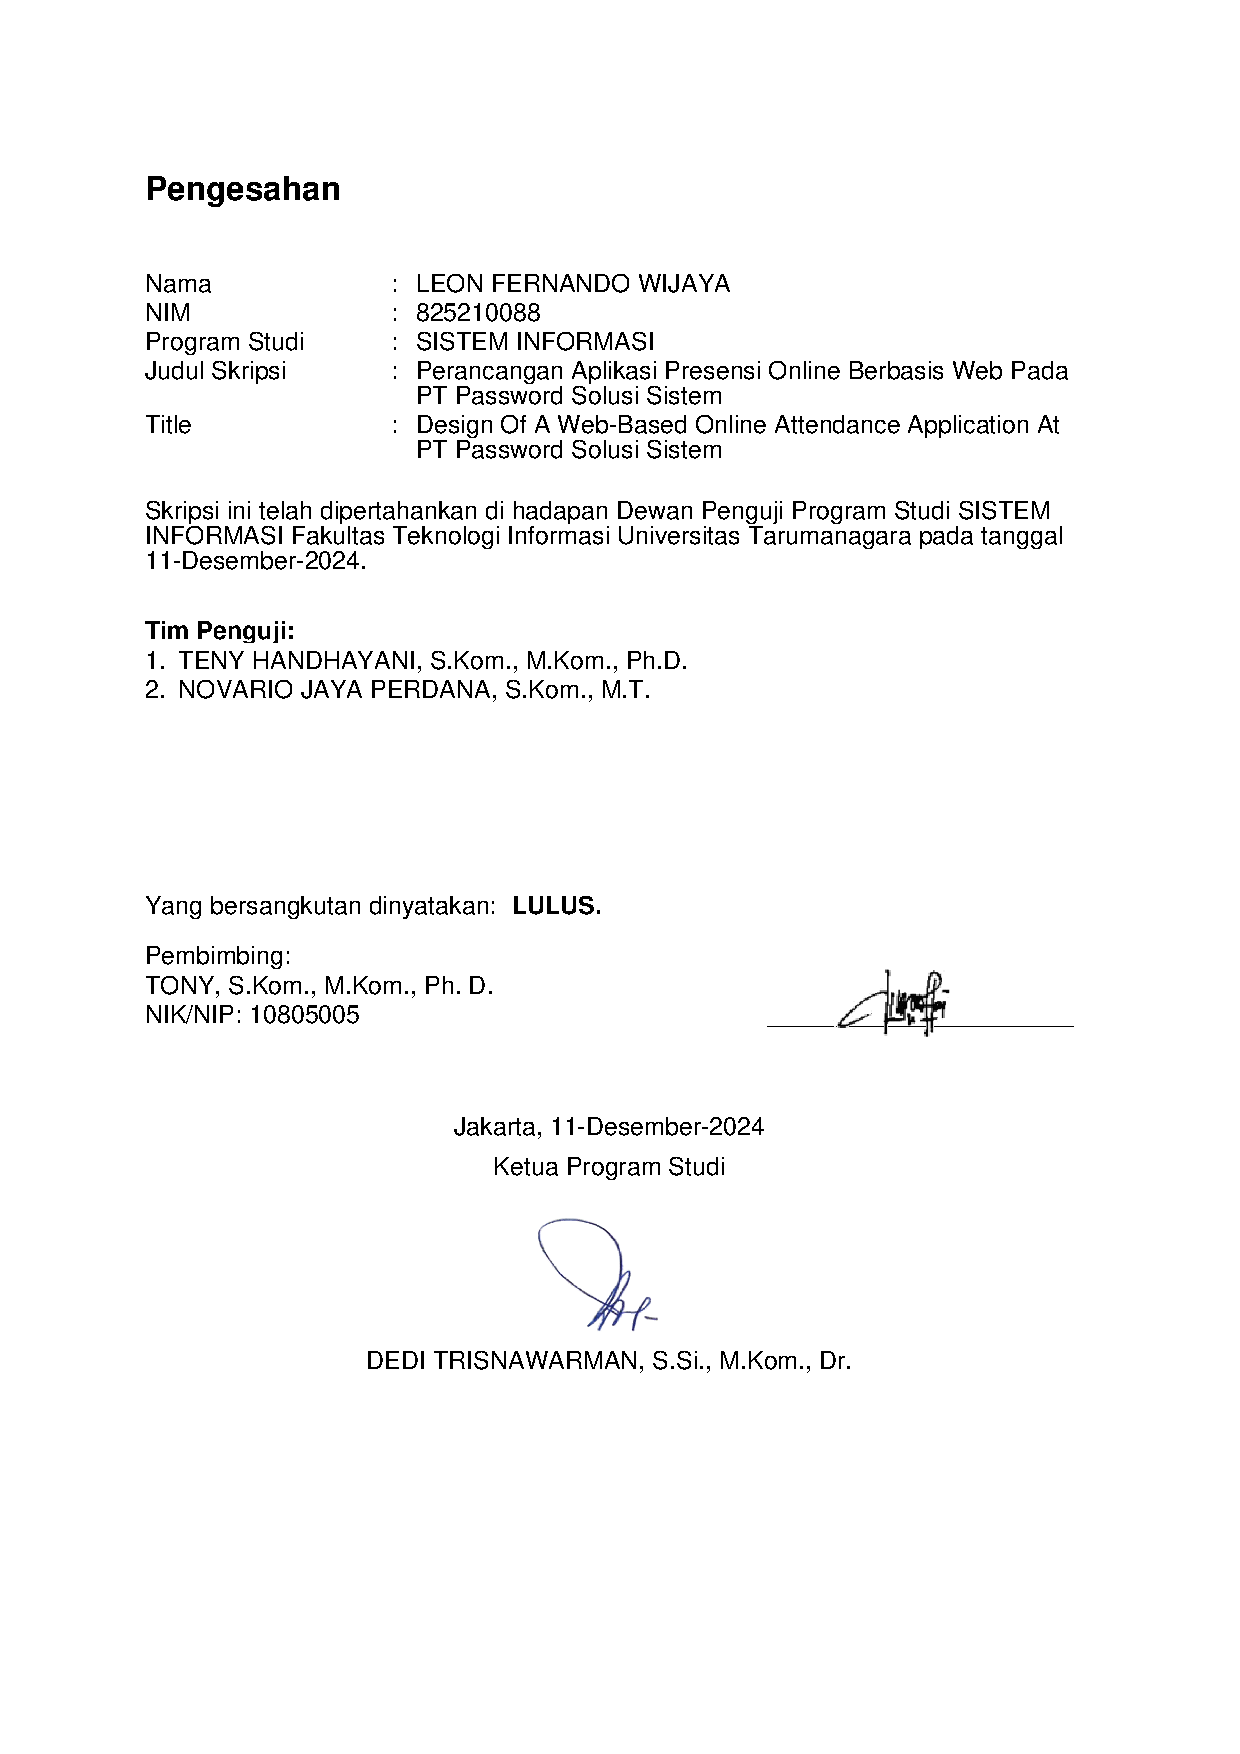
\includegraphics[page=1, scale=3, width=17cm, trim={0cm 2cm 0cm 2cm}, clip]{Header/pengesahan-skripsi.pdf}
\end{figure}
\FloatBarrier
\end{center}


\chapter*{\centering }

\setstretch{1.5}
\thispagestyle{empty}

\addcontentsline{toc}{chapter}{LEMBAR PERNYATAAN}
\begin{center}
    % \vspace{0.75cm}
    \begin{figure}[!htbp]
	\centering
		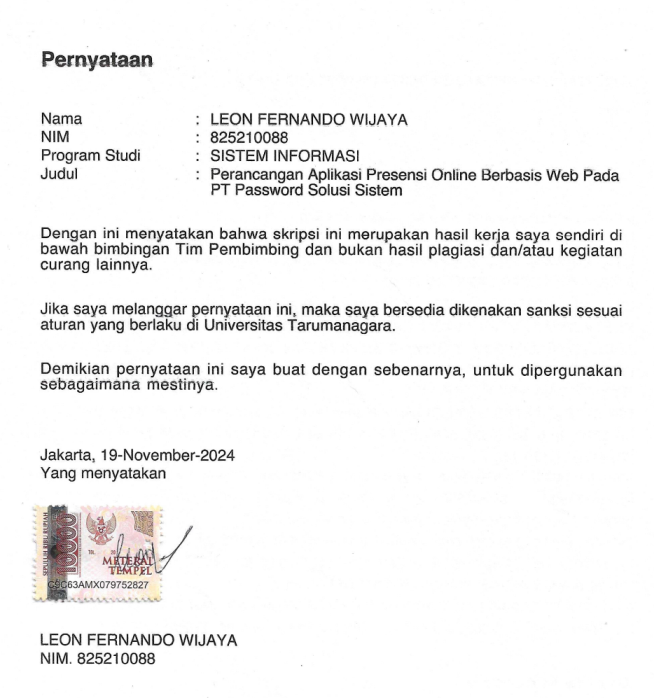
\includegraphics[width=0.9\textwidth]{Header/pernyataan.png}
\end{figure}
\FloatBarrier
    % 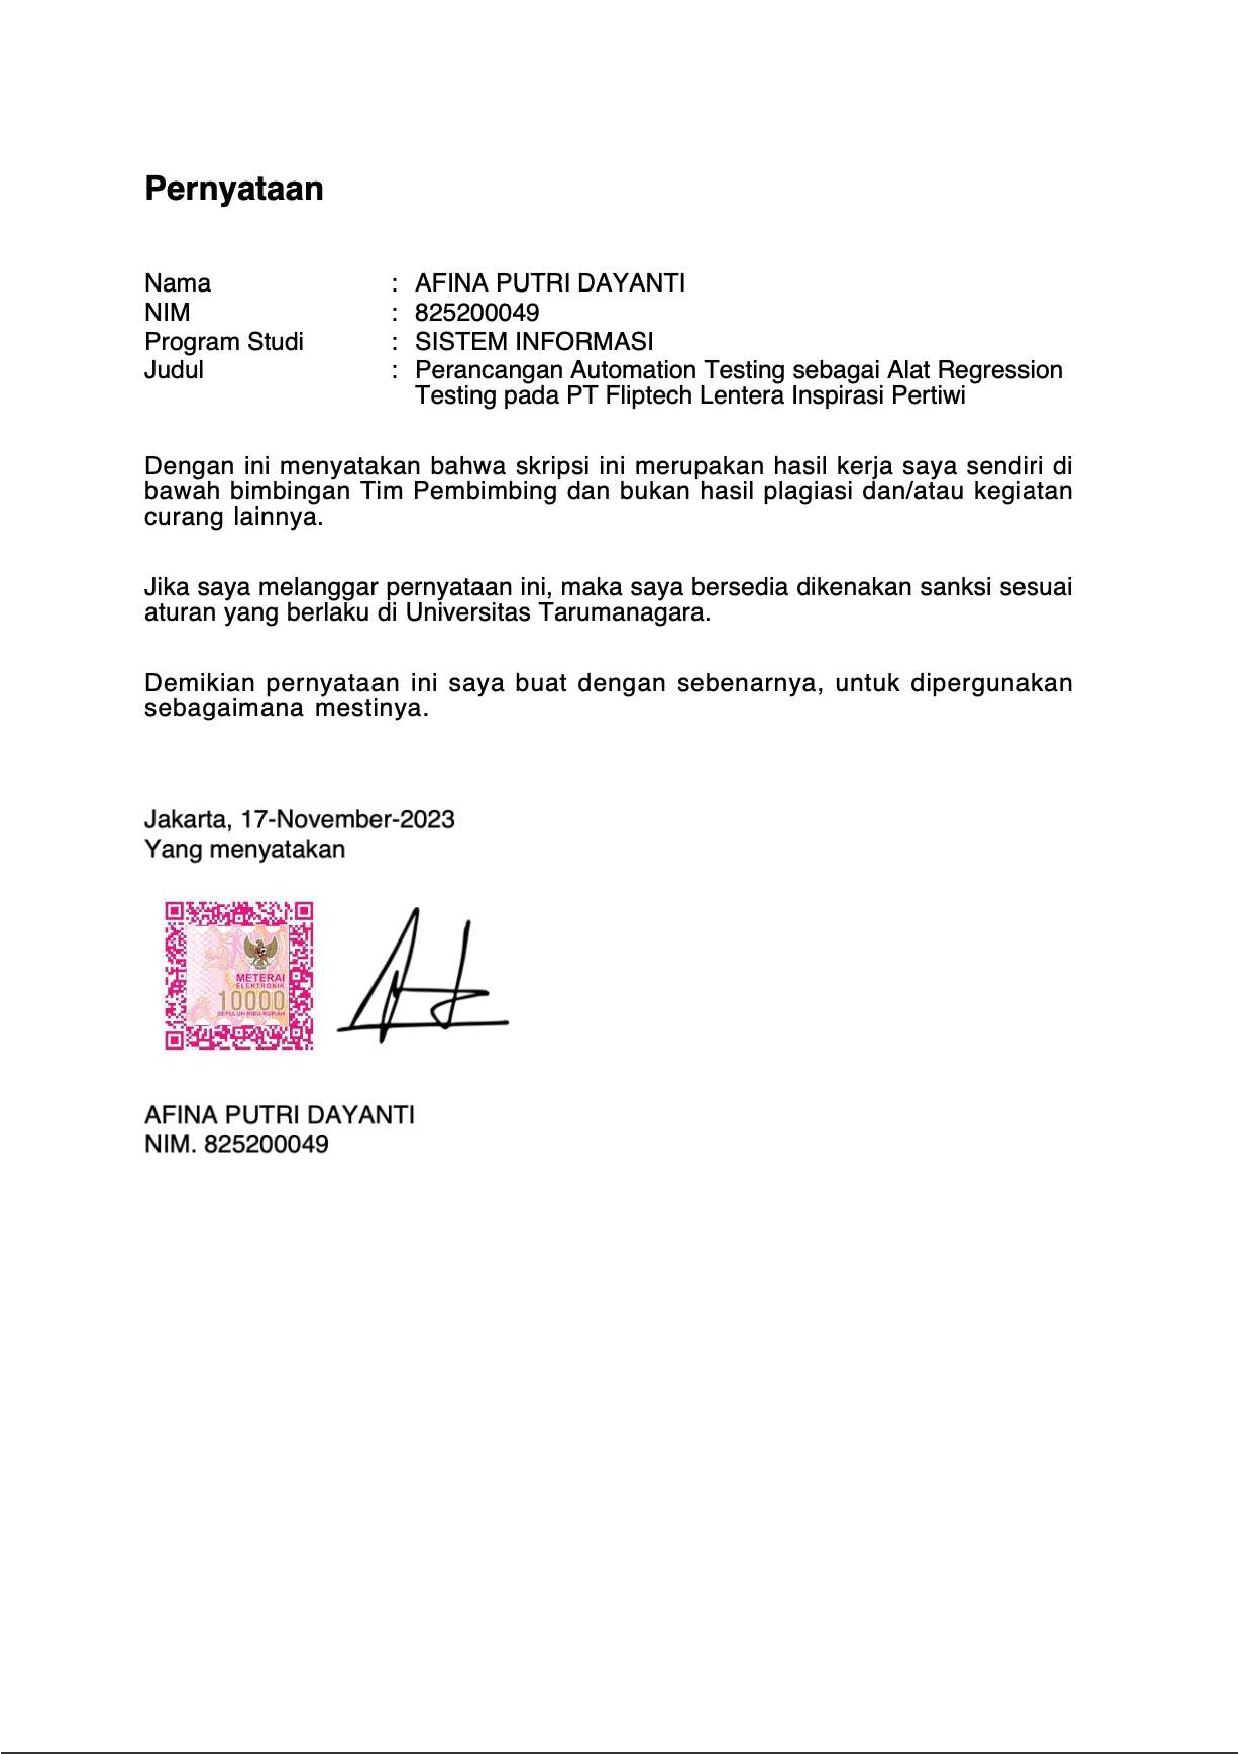
\includegraphics[page=1, scale=3, width=17cm, trim={2cm 7cm 2cm 2cm}, clip]{Header/pernyataan_825200049.pdf}
\end{center}


\chapter*{\centering ABSTRAK}
\addcontentsline{toc}{chapter}{ABSTRAK}

\begin{spacing}{1}
\noindent MyPassword adalah perusahaan penyedia solusi teknologi informasi dan integrator sistem, yang menawarkan solusi infrastruktur TI dan aplikasi bisnis. Perusahaan ini terdiri dari beberapa divisi, termasuk \textit{Business Application}, \textit{Infrastructure}, \textit{Human Resources}, dan \textit{Business Support}. Salah satu tantangan yang saat ini dihadapi oleh tim \textit{Human Resources} adalah sistem pengajuan lembur di divisi \textit{Infrastructure}. Saat ini, perusahaan sudah memiliki aplikasi presensi yang memiliki fitur pengajuan lembur. Namun, aplikasi saat ini masih kurang efisien dalam proses pencatatan lembur dan aplikasi tidak bisa dikustomisasi sesuai kebutuhan perusahaan, karena fitur-fiturnya sudah ditentukan oleh pihak eksternal yang mengembangkan aplikasi tersebut. Tim \textit{Human Resources} menginginkan sistem aplikasi yang mampu mencatat dan menghitung lembur secara otomatis ketika \textit{staff} melakukan presensi diluar jam \textit{shift} atau hari libur yang ditetapkan perusahan, baik untuk WFO maupun WFH. Oleh karena itu, dikembangkanlah aplikasi presensi \textit{online} berbasis web dengan menggunakan bahasa PHP dan \textit{framework} Laravel, serta MySQL sebagai basis datanya. Aplikasi presensi \textit{online} berbasis web akan dikembangkan dengan metode Scrum. Aplikasi presensi \textit{online} menggunakan teknik Geolocation untuk mengambil titik koordinat lokasi \textit{staff} ketika melakukan presensi. Titik koordinat yang didapat akan dikonversi menjadi peta interaktif dan nama lengkap jalan. Aplikasi presensi \textit{online} juga mengimplementasikan algoritma Haversine untuk menghitung jarak antara lokasi \textit{staff} saat presensi dengan lokasi kantor MyPassword, hasil perhitungan untuk memberikan keterangan saat presensi. Selain itu, aplikasi juga dilengkapi TensorFlow untuk melakukan validasi wajah saat pengambilan foto presensi. Pengujian fitur aplikasi presensi \textit{online} juga dilakukan oleh \textit{programmer} menggunakan metode \textit{whitebox testing}, sedangkan pengujian oleh \textit{user} menggunakan \textit{blackbox testing}. Pengujian oleh \textit{programmer} akan dilakukan pengujian keseluruhan fitur dari aplikasi termasuk pengujian perhitungan algoritma Haversine. Pengujian perhitungan algoritma Haversine dilakukan dengan membandingkannya terhadap perhitungan \textit{Google Geometry} API pada 20 titik lokasi berbeda. Hasilnya menunjukkan rata-rata perbedaan sebesar 0.0113 km. Selain itu, pengujian oleh \textit{user} akan dilakukan oleh \textit{Staff Infrastructure, Manager Infrastructure}, dan \textit{Manager Human Resources} untuk menguji seluruh fitur sesuai dengan masing-masing \textit{role}. Hasil dari pengujian oleh \textit{programmer} maupun \textit{user} mendapatkan hasil \textit{valid} untuk seluruh \textit{test case}. Pengujian juga dilakukan kepada 10 \textit{staff non-}IT menggunakan metode \textit{blackbox testing} yang mendapatkan hasil valid untuk semua skenario dan pengujian SUS juga dilakukan yang mendapatkan hasil skor 79,5 yang merupakan peringkat A- dalam pengujian SUS.     
\\


 

\noindent\textbf{Kata kunci:} Presensi, lembur, \textit{geolocation}, \textit{framework} Laravel, scrum
\end{spacing}




% \chapter*{\centering ABSTRACT}
\addcontentsline{toc}{chapter}{ABSTRACT}

\begin{spacing}{1.25}

\end{spacing}
\chapter*{\centering KATA PENGANTAR}
\addcontentsline{toc}{chapter}{KATA PENGANTAR}

Puji syukur kehadirat Tuhan Yang Maha Esa yang telah melimpahkan rahmat dan karunia-Nya sehingga penulis dapat menyelesaikan skripsi ini dengan judul “Perancangan Aplikasi Presensi \textit{Online} berbasis \textit{Web} pada PT Password Solusi Sistem”. Skripsi ini disusun sebagai salah satu syarat untuk memperoleh gelar Sarjana pada Program Studi sistem Informasi, Fakultas Teknologi Informasi, Universitas Tarumanagara.

Penulis menyadari bahwa penyusunan skripsi ini tidak terlepas dari bantuan, bimbingan, dan dukungan dari berbagai pihak. Oleh karena itu, penulis ingin menyampaikan ucapan terima kasih yang sebesar-besarnya kepada:

\begin{enumerate}
\item Ibu Prof. Dr. Ir. Dyah Erny Herwindiati, M.Si., selaku Dekan Fakultas Teknologi Informasi Universitas Tarumanagara.

\item Bapak Dr. Dedi Trisnawarman, S.Si., M.Kom., selaku Ketua Program Studi Sistem Informasi Universitas Tarumanagara.

\item Bapak Novario Jaya Perdana, S.Kom., MT, selaku Sekretaris Program Studi Sistem Informasi Universitas Tarumanagara.

\item Bapak Wasino, S.Kom., M.Kom, selaku Koordinator Skripsi sekaligus Ketua Bidang Kajian \textit{Enterprise Database} pada Program Studi Sistem Informasi Universitas Tarumanagara.

\item Bapak Tony, Ph.D., selaku dosen pembimbing skripsi yang telah memberikan arahan, bimbingan, dan inspirasi kepada penulis.

\item Ibu Melissa, selaku \textit{Manager Human Resources Development} di MyPassword, yang telah memberikan kesempatan kepada penulis untuk melakukan penelitian skripsi di perusahaan.

\item Bapak Yehuda Chaniago, selaku \textit{Manager Business Application} di MyPassword, yang telah memberikan bantuan, saran, dan masukkan kepada penulis saat melakukan penelitian skripsi di perusahaan.

\item Keluarga penulis, yang selalu memberikan doa, dukungan, dan kasih sayang yang tiada henti.

\end{enumerate}

Penulis menyadari bahwa skripsi ini masih memiliki ruang untuk perbaikan dan peningkatan. Kritik dan saran dari pembaca sangat diharapkan agar penulisan selanjutnya dapat lebih baik lagi. Semoga penelitian dan perancangan ini dapat memberikan manfaat dan wawasan bagi pembaca. Akhir kata, penulis berdoa agar Tuhan Yang Maha Esa senantiasa memberikan keberkahan dan rahmat untuk kita semua.

\vspace{0.2in}
\begin{flushright}
Jakarta, 20 November \the\year{}\\
Penulis \\
\begin{figure}[htbp]
	\flushright
	
\includegraphics[width=3cm]{Gambar/signed-leon.png}
\end{figure}
(Leon Fernando Wijaya)
\end{flushright}

% \chapter*{\centering ABSTRACT}
\addcontentsline{toc}{chapter}{ABSTRACT}

\begin{spacing}{1.25}

\end{spacing}
\input{Header/daftar-isi}
\chapter*{\centerline{DAFTAR TABEL}}
\addcontentsline{toc}{chapter}{DAFTAR TABEL}

\makeatletter

\renewcommand{\numberline}[1]{%
  \hb@xt@1.5em{#1.\hfil}%
  \hspace{3em} % Menambah spasi 4em antara nomor dan judul gambar
}

\@starttoc{lot}
\makeatother

\newpage
\chapter*{\centerline{DAFTAR GAMBAR}}
\addcontentsline{toc}{chapter}{DAFTAR GAMBAR}

\makeatletter


\renewcommand{\numberline}[1]{%
  \hb@xt@1.5em{#1.\hfil}%
  \hspace{4em} % Menambah spasi 4em antara nomor dan judul gambar
}


\@starttoc{lof}


\makeatother

\newpage

% \chapter*{\centerline{DAFTAR KODE}}
\addcontentsline{toc}{chapter}{DAFTAR KODE}

\makeatletter
\@starttoc{lol}
\makeatother

\newpage

\chapter{\vspace{2ex}PENDAHULUAN}
\pagenumbering{arabic}

\section{Latar Belakang Masalah}
Pusat Data dan Informasi (Pusdatin) Universitas Tarumanagara (UNTAR) merupakan unit pengelola infrastruktur teknologi informasi dan sistem data terpusat yang mendukung seluruh kegiatan operasional akademik maupun administratif di lingkungan universitas. Seiring berjalannya waktu dan terus meningkatnya jumlah mahasiswa yang terdaftar serta transaksi akademik yang terjadi setiap semester, volume data yang tersimpan di dalam basis data produksi (\textit{active database}) mengalami pertumbuhan yang sangat signifikan dan pesat. Akumulasi data historis ini mencakup rekam jejak akademik, transkrip nilai, data kehadiran, hasil evaluasi pembelajaran, hingga log transaksi operasional mahasiswa dari seluruh angkatan tahun-tahun sebelumnya.

Penumpukan data historis mahasiswa dengan volume yang sangat besar dalam satu basis data produksi utama menimbulkan beberapa kendala krusial yang berdampak langsung pada operasional harian Pusdatin UNTAR. Pertama, kapasitas ruang penyimpanan (\textit{storage space}) pada basis data produksi kian terbatas dan terbebankan secara tidak proporsional oleh data historis yang sudah jarang diakses secara langsung dalam kegiatan operasional harian. Kedua, akumulasi tabel yang terus membengkak berdampak langsung pada penurunan efisiensi dan performa eksekusi kueri (\textit{query performance}) untuk layanan transaksi aktif mahasiswa, dosen, maupun staf administrasi. Di sisi lain, data historis mahasiswa tersebut sama sekali tidak dapat dihapus secara permanen (\textit{hard delete}) karena terikat oleh kebutuhan regulatori, kebijakan retensi dokumen akademik universitas, serta kewajiban pemenuhan kepatuhan audit internal maupun eksternal yang bersifat jangka panjang \cite{zulkifli2011manajemen}.

Selain masalah performa kueri dan keterbatasan ruang penyimpanan, kendala signifikan juga ditemukan pada proses pencadangan data (\textit{data backup}) yang berjalan saat ini di Pusdatin UNTAR. Proses pencadangan dilakukan secara menyeluruh (\textit{full database backup}) yang mencakup gabungan antara data transaksi aktif dan data historis secara terkonsolidasi pada satu server utama. Pendekatan ini membutuhkan durasi waktu yang sangat lama (\textit{time-consuming}) serta memerlukan alokasi sumber daya komputasi yang tinggi, sehingga dinilai kurang efisien dan berpotensi meningkatkan risiko kegagalan proses pencadangan pada saat terjadi lonjakan transaksi operasional.

Lebih lanjut, ketika unit terkait seperti Biro Administrasi Akademik atau tim auditor memerlukan data historis mahasiswa tertentu untuk keperluan pelaporan maupun pemeriksaan, tidak terdapat mekanisme yang terstruktur dan cepat untuk menemukannya. Pencarian manual yang dilakukan langsung pada basis data produksi berisiko mengganggu kinerja sistem transaksi aktif yang sedang berjalan, sekaligus berpotensi mengekspos integritas data operasional terhadap perubahan yang tidak terotorisasi \cite{james2014database}.

Guna mengatasi permasalahan tersebut secara sistematis, diperlukan perancangan mekanisme pengarsipan data (\textit{data archiving}) otomatis yang mampu memisahkan data historis mahasiswa dari basis data produksi ke dalam basis data arsip yang terpisah secara terjadwal dan terkonfigurasi. Sistem pengarsipan ini dirancang dengan arsitektur \textit{Client-Worker} terdistribusi yang berkomunikasi melalui HTTP API JSON (\textit{agent.ashx}), di mana eksekusi antrean tugas (\textit{task queue}) dijalankan oleh SQL Server Agent dan skrip PowerShell pada mesin eksternal terpisah. Dengan arsitektur ini, beban komputasi proses pengarsipan tidak langsung menimpa infrastruktur server kampus yang kapasitasnya terbatas. Sistem ini juga dilengkapi dengan portal \textit{on-demand retrieval} berbasis \textit{web} ASP.NET yang memungkinkan staf dan unit terkait di Pusdatin UNTAR melakukan pencarian dan penarikan data historis secara cepat dan akurat lintas basis data---baik pada basis data aktif maupun basis data arsip---tanpa membebani basis data produksi utama.

Berdasarkan uraian permasalahan dan gagasan solusi di atas, penulis mengangkat penelitian skripsi dengan judul \textbf{"PERANCANGAN APLIKASI DATA \textit{ARCHIVING} OTOMATIS DAN PORTAL \textit{ON-DEMAND RETRIEVAL} BERBASIS WEB ASP.NET PADA PUSDATIN UNTAR"}. Penelitian ini diharapkan dapat membantu Pusdatin UNTAR dalam meningkatkan efisiensi penyimpanan data, mengoptimalkan kecepatan proses pencadangan, serta mempercepat akses penarikan data historis mahasiswa sesuai kebutuhan audit, regulasi, dan pelayanan akademik yang berlaku.


\section{Rumusan Masalah}
Berdasarkan latar belakang masalah yang telah diuraikan, rumusan masalah dalam penelitian ini adalah sebagai berikut:
\begin{enumerate}
    \item Bagaimana merancang alur kerja (\textit{workflow}) pemindahan data historis mahasiswa secara otomatis dari basis data produksi ke basis data arsip, guna mengoptimalkan kinerja eksekusi kueri dan efisiensi ruang penyimpanan pada Pusdatin UNTAR?

    \item Bagaimana membangun portal \textit{web} berbasis ASP.NET yang memfasilitasi pencarian dan penarikan data secara \textit{on-demand} (\textit{on-demand retrieval}) secara fleksibel lintas basis data, baik basis data aktif maupun basis data arsip, tanpa mengganggu kinerja sistem produksi?

    \item Bagaimana merancang dan mengimplementasikan arsitektur \textit{Client-Worker} terdistribusi berbasis HTTP API JSON (\textit{agent.ashx}) yang dieksekusi melalui SQL Server Agent dan skrip PowerShell pada mesin eksternal terpisah, guna menjalankan antrean tugas (\textit{task queue}) pengarsipan data tanpa membebani infrastruktur server utama kampus?
\end{enumerate}


\section{Batasan Masalah}
Dalam perancangan dan pengembangan aplikasi pengarsipan data otomatis serta portal \textit{on-demand retrieval} ini, terdapat beberapa batasan masalah yang ditetapkan sebagai fokus penelitian, antara lain:
\begin{enumerate}
    \item Rentang waktu dan kriteria pengarsipan data historis mahasiswa---baik berdasarkan Tahun Akademik, Nomor Induk Mahasiswa (NIM), maupun parameter akademik lainnya---bersifat dinamis dan fleksibel sesuai dengan konfigurasi sistem yang dapat diatur oleh administrator. Kriteria pengarsipan tidak terikat pada aturan baku jangka waktu tertentu, melainkan dapat disesuaikan dengan kebijakan operasional Pusdatin UNTAR yang berlaku pada saat implementasi.

    \item Eksekusi pemindahan data tidak dilakukan secara langsung pada server utama Pusdatin UNTAR melalui eksekusi lokal, melainkan menggunakan arsitektur \textit{Client-Worker} terdistribusi yang berkomunikasi melalui layanan HTTP API JSON (\textit{agent.ashx}). Mekanisme ini memisahkan tanggung jawab inisiasi tugas (\textit{client}) dari eksekusi pemindahan data aktual (\textit{worker}) secara terstruktur.

    \item Eksekusi antrean tugas (\textit{task queue}) pengarsipan dijalankan menggunakan SQL Server Agent dan skrip PowerShell yang dipasang pada mesin terpisah (laptop eksternal / \textit{external machine}) yang bertindak sebagai \textit{primary agent}. Pendekatan ini dipilih secara khusus untuk mengatasi batasan infrastruktur dan kapasitas komputasi pada server kampus Pusdatin UNTAR yang tidak memungkinkan penggunaan mekanisme penjadwalan lokal secara langsung.

    \item Portal \textit{web} pengarsipan dan pencarian data dikembangkan menggunakan kerangka kerja ASP.NET (C\# / Web Forms) dan terintegrasi dengan basis data Microsoft SQL Server sebagai sistem manajemen basis data utama.

    \item Seluruh proses pengujian fungsionalitas dan validasi sistem aplikasi---mencakup pengujian alur pemindahan data, pengujian antrean tugas, serta pengujian pencarian \textit{on-demand}---sepenuhnya dieksekusi di dalam lingkungan pengembangan dan uji coba (\textit{development/staging environment}), bukan pada basis data produksi Pusdatin UNTAR yang sedang berjalan secara langsung.
\end{enumerate}


\section{Tujuan dan Manfaat}
\subsection{Tujuan}
Tujuan dari penelitian dan perancangan aplikasi ini adalah:
\begin{enumerate}
    \item Merancang aplikasi pengarsipan data (\textit{data archiving}) otomatis dengan arsitektur \textit{Client-Worker} terdistribusi melalui HTTP API JSON (\textit{agent.ashx}) guna memindahkan data historis dari basis data produksi ke basis data arsip.
    
    \item Membangun portal \textit{web} berbasis ASP.NET yang menyediakan layanan \textit{on-demand retrieval} untuk memfasilitasi pencarian dan penarikan data historis lintas basis data secara fleksibel dan cepat.

    \item Mengimplementasikan sistem antrean tugas (\textit{task queue}) menggunakan SQL Server Agent dan skrip PowerShell pada mesin eksternal terpisah guna menjalankan eksekusi pemindahan data tanpa membebani infrastruktur server utama Pusdatin UNTAR.
\end{enumerate}

\subsection{Manfaat}
Manfaat yang diharapkan dari hasil penelitian ini antara lain:
\begin{enumerate}
    \item **Bagi Pusdatin UNTAR**: Meningkatkan performa eksekusi kueri operasional harian dan efisiensi ruang penyimpanan pada basis data produksi melalui pengurangan beban akumulasi data historis.

    \item **Bagi Sistem dan Infrastruktur**: Mempercepat proses pencadangan data (\textit{backup process}) karena ukuran basis data produksi aktif menjadi lebih kecil dan efisien untuk dicadangkan.

    \item **Bagi Layanan Akademik dan Audit**: Memudahkan staf operasional dalam memenuhi kebutuhan penarikan data historis mahasiswa secara cepat saat diperlukan untuk keperluan regulasi maupun audit internal/eksternal.
\end{enumerate}

\section{Metodologi}
Metodologi yang digunakan dalam pengembangan aplikasi pengarsipan data otomatis dan portal \textit{on-demand retrieval} ini mengacu pada tahapan \textit{System Development Life Cycle} (SDLC) yang terstruktur, meliputi langkah-langkah sebagai berikut:

\begin{enumerate}
    \item \textbf{Tahap Analisis Kebutuhan (\textit{Requirements Analysis}):}
    \\ Melakukan analisis terhadap struktur basis data produksi Pusdatin UNTAR, identifikasi data historis mahasiswa, penetapan kriteria pengarsipan dinamis, serta formulasi spesifikasi titik akhir HTTP API JSON (\textit{agent.ashx}).

    \item \textbf{Tahap Perancangan Sistem (\textit{System Design}):}
    \\ Merancang arsitektur terdistribusi \textit{Client-Worker}, alur alokasi \textit{task queue}, struktur tabel basis data arsip, mekanisme komunikasi API JSON, serta tata letak antarmuka (\textit{User Interface}) portal \textit{web} ASP.NET.

    \item \textbf{Tahap Konstruksi dan Implementasi (\textit{Implementation}):}
    \\ Membangun portal \textit{web} menggunakan ASP.NET (C\# / Web Forms), mengembangkan modul HTTP Handler (\textit{agent.ashx}), serta menyusun skrip eksekusi PowerShell dan penjadwalan tugas pada SQL Server Agent di mesin \textit{worker} eksternal.

    \item \textbf{Tahap Pengujian (\textit{Testing}):}
    \\ Melaksanakan pengujian fungsionalitas dan integrasi secara komprehensif pada lingkungan pengembangan (\textit{development/staging environment}) untuk memastikan integritas pemindahan data dan keandalan pencarian \textit{on-demand retrieval}.

    \item \textbf{Tahap Evaluasi dan Dokumentasi (\textit{Evaluation \& Documentation}):}
    \\ Menganalisis hasil pengujian sistem, menyusun dokumentasi teknis penggunaan aplikasi, serta mendokumentasikan seluruh proses ke dalam Laporan Skripsi.
\end{enumerate}

\section{Lokasi dan Waktu Pelaksanaan}
Penelitian dan perancangan aplikasi ini dilaksanakan di Pusat Data dan Informasi (Pusdatin) Universitas Tarumanagara (UNTAR), yang beralamat di Jalan Letjen S. Parman No. 1, Grogol Petamburan, Jakarta Barat. Waktu pelaksanaan perancangan dan penyusunan skripsi ini berlangsung pada Semester Genap Tahun Akademik 2025/2026 (Tahun 2026).

\section{Sistematika Penulisan}
Penyusunan laporan skripsi ini dibagi menjadi lima bab utama yang saling terhubung dengan sistematika sebagai berikut:

\noindent\textbf{BAB 1 PENDAHULUAN}
\\ Menguraikan latar belakang masalah mengenai beban akumulasi data historis mahasiswa di Pusdatin UNTAR, rumusan masalah, batasan masalah terkait kriteria dinamis dan arsitektur terdistribusi \textit{Client-Worker}, tujuan dan manfaat penelitian, metodologi SDLC yang digunakan, lokasi dan waktu pelaksanaan, serta sistematika penulisan.

\noindent\textbf{BAB 2 DASAR TEORETIS, METODOLOGI, PERANCANGAN}
\\ Menyajikan kajian pustaka dan dasar teori yang relevan meliputi konsep \textit{data archiving}, \textit{on-demand retrieval}, arsitektur ASP.NET Web Forms, komunikasi HTTP API JSON (\textit{agent.ashx}), pemrosesan skrip PowerShell, serta fitur automatisasi SQL Server Agent. Bab ini juga memuat perancangan arsitektur terdistribusi, perancangan basis data arsip, dan rancangan antarmuka portal \textit{web}.

\noindent\textbf{BAB 3 PEMBUATAN DAN IMPLEMENTASI}
\\ Membahas kebutuhan perangkat lunak dan keras pada lingkungan \textit{development/staging}, tahap pembuatan modul \textit{handler} API JSON, konfigurasi tugas penjadwalan pada SQL Server Agent dan PowerShell \textit{worker}, serta pembuatan halaman portal \textit{web} ASP.NET untuk pencarian data.

\noindent\textbf{BAB 4 PENGUJIAN DAN PEMBAHASAN}
\\ Menjelaskan hasil pengujian fungsionalitas dan performa sistem pada lingkungan pengembangan, analisis kecepatan pemindahan data historis, validasi pencarian data lintas basis data, serta pembahasan terhadap pencapaian solusi yang dirancang.

\noindent\textbf{BAB 5 KESIMPULAN DAN SARAN}
\\ Menyajikan kesimpulan akhir berdasarkan hasil pengujian dan pembahasan yang telah dilakukan, serta memberikan saran-saran akademis maupun praktis untuk pengembangan sistem pengarsipan di masa mendatang.
\chapter{\vspace{2ex}DASAR TEORITIK, METODOLOGI, DAN PERANCANGAN}

\section{Teori Dasar}
\subsection{Presensi}
Menurut Kamus Besar Bahasa Indonesia (KBBI)~\cite{kbbionline}, presensi diartikan sebagai kehadiran. Kehadiran itu sendiri mengacu pada kehadiran individu atau kelompok di suatu tempat untuk mengikuti acara yang telah direncanakan sebelumnya. Kehadiran karyawan berperan penting dalam menentukan kinerja mereka dalam menyelesaikan tugas~\cite{narulita2024buku}.

\subsection{Aplikasi Presensi}
Aplikasi adalah perangkat lunak yang dirancang untuk menjalankan tugas tertentu pada sistem komputer. Dalam pengembangannya, aplikasi dikategorikan menjadi 3 yaitu aplikasi web, aplikasi \textit{desktop}, dan aplikasi \textit{mobile}.~\cite{pane2020membangun}. Sedangkan, presensi merupakan kehadiran. Maka aplikasi presensi dapat disebut sebagai perangkat lunak yang digunakan untuk mencatat dan memantau kehadiran suatu individu. Menurut Imaniawan dan Rijanandi~\cite{imaniawan2023presensi}, aplikasi presensi memungkinkan pengelolaan data kehadiran secara efisien dikarenakan data dari presensi langsung tersimpan pada server.

\subsection{Lembur}
Menurut Kamus Besar Bahasa Indonesia (KBBI)~\cite{kbbionline}, Lembur merupakan pekerjaan dinas yang dilakukan diluar jam dinas. Berdasarkan Keputusan Menteri Tenaga Kerja Republik Indonesia Nomor KEP. 102 Men VI 2004 pasal 1~\cite{menteri2014peraturan}, perusahaan diwajibkan untuk membayar upah lembur kepada pegawai jika masuk pada kategori berikut:
\begin{enumerate}
    \item Bekerja lebih dari 7 jam dalam sehari atau 40 jam dalam seminggu untuk pegawai yang bekerja selama 6 hari.
    \item Bekerja lebih dari 8 jam sehari dan 40 jam dalam seminggu untuk pegawai yang bekerja selama 5 hari.
    \item Bekerja pada hari istirahat mingguan dan hari libur nasional.
\end{enumerate}

\subsection{\textit{Geolocation}}
Menurut Shellito~\cite{introduction2019bradley}, \textit{Geolocation} adalah teknik yang digunakan untuk menentukan lokasi suatu perangkat di dunia nyata, seperti \textit{smartphone}, tablet, atau komputer. Dengan \textit{Geolocation}, perangkat dapat mengetahui koordinatnya (lintang dan bujur) melalui berbagai metode, seperti alamat IP, koneksi Wi-Fi, menara seluler, atau GPS. Setelah lokasi ditentukan, informasi tersebut dapat dipetakan dan dibagikan melalui internet.

\subsection{Haversine}
Haversine merupakan metode paling populer yang menggunakan trigonometri untuk menghitung jarak lingkaran besar dengan menggunakan koordinat yang didefinisikan dalam derajat desimal sebagai \textit{input}. Rumus Haversine adalah rumus pengukuran jarak yang paling umum digunakan karena relatif ringan dari segi pengkodean dan cukup akurat dalam kebanyakan kasus~\cite{learning2019joel}. Menurut Xiao~\cite{gis2015xiao}, langkah pertama pada rumus Haversine yaitu mencari nilai a atau nilai antara yang dapat dilihat pada \textbf{Persamaan \ref{eq:nilai-a}}.
\begin{equation}
    a = \sin^2 \left( \frac{d\varphi}{2} \right) + \cos(\varphi_1) \cdot \cos(\varphi_2) \cdot \sin^2 \left( \frac{d\lambda}{2} \right)
\label{eq:nilai-a}
\end{equation}


\noindent Keterangan:
\\
$d\varphi$ = Perbedaan lintang antara dua titik ($\varphi_2 - \varphi_1$).
\\
$\varphi_1$ = Lintang titik pertama (dalam radian).
\\
$\varphi_2$ = Lintang titik kedua (dalam radian).
\\
$d\lambda$ = Perbedaan bujur antara dua titik ($\lambda_2 - \lambda_1$).
\\
$\lambda_1$ = Bujur titik pertama (dalam radian).
\\
$\lambda_2$ = Bujur titik kedua (dalam radian).
\\

Selanjutnya, mencari nilai c atau jarak sudut antara dua titik pada permukaan bola dalam radian menggunakan nilai a yang sudah didapatkan sebelumnya yang dapat dilihat pada \textbf{Persamaan \ref{eq:nilai-c}}.
\begin{equation}
    c = 2 \, \text{arcsin} \left( \min(1, \sqrt{a}) \right)
\label{eq:nilai-c}
\end{equation}

Setelah itu, mencari nilai d atau jarak sebenarnya antara dua titik dalam permukaan bumi dengan mengalikan nilai jarak sudut (c) dengan jari-jari bumi (6371 km) yang dapat dilihat pada \textbf{Persamaan \ref{eq:nilai-d}}.
\begin{equation}
    d = cR
\label{eq:nilai-d}
\end{equation}

Berikut ini adalah contoh perhitungan manual menggunakan rumus Haversine antara titik koordinat Universitas Tarumanagara (-6.19058187063816, 106.79779495106814) dengan titik koordinat MyPassword (-6.169336170685656, 106.78859045462738). Langkah pertama adalah melakukan konversi lintang dan bujur kedua titik menjadi radian dan mencari nilai perbedaan lintang dan bujur antara dua titik.
\\
$\varphi_1 = -6,19058187063816 \cdot \left( \frac{\pi}{180} \right) = -0.10804603626 $ radian 
\\
$\lambda_1 = 106,79779495106814 \cdot \left( \frac{\pi}{180} \right) = 1,86397315577 $ radian
\\
$\varphi_2 = -6,169336170685656 \cdot \left( \frac{\pi}{180} \right) = -0,10767522884 $ radian
\\
$\lambda_2 = 106,78859045462738 \cdot \left( \frac{\pi}{180} \right) = 1,86381250700 $ radian
\\
$d\varphi = -0,10767522884 - (-0,10804603626) = 0,00037080742 $ radian
\\
$d\lambda = 1,86381250700 - 1,86397315577 = -0,00016064877 $ radian
\\


Setelah melakukan pengubahan semua lintang dan bujur menjadi radian. Selanjutnya, melakukan perhitungan untuk mencari nilai $c$ atau jarak sudut antara dua titik.
\\
$a = \sin^2 \left( \frac{0,00037080742}{2} \right) + \cos(-0.10804603626) \cdot \cos(-0,10767522884) \cdot \sin^2 \left( \frac{-0,00016064877}{2} \right)$
\\
$a = (0,0001854037)^2 + 0,99416870319 \cdot 0,9942086212 \cdot  (-0,00008032438)^2 $
\\
$a = 3,4374535 $ x $10^-8$ + $0,99416870319 \cdot 0,9942086212 \cdot 6,452007$ x $10^-9 $
\\
$a = 4,0751770 $ x $ 10^-8 $
\\


Selanjutnya menghitung nilai c atau jarak sudut antara dua titik menggunakan nilai a atau nilai antara yang sudah didapatkan sebelumnya.
\\
$c = 2 \cdot \, \text{arcsin} \left( \min(1, \sqrt{4,0751770 \, \text{x} \, 10^-8}) \right)$
\\
$c = 2 \cdot \, \text{arcsin} \, 0,00020187066 $
\\
$c = 0,00040374135 $
\\

Terakhir, menghitung jarak dua titik dalam permukaan bumi menggunakan nilai c atau jarak sudut antara dua titik dengan jari-jari bumi (6371 km).
\\
$d = 0,00040374135 \cdot 6371 $
\\
$d = 2,5722361635632 $
\\


Jadi, hasil jarak yang dihitung antara Universitas Tarumanagara dan MyPassword menggunakan rumus Haversine adalah 2,57 km.



\subsection{\textit{World Wide Web} atau Web}
\textit{World Wide Web} (WWW) atau Web adalah sebuah aplikasi perangkat lunak yang memudahkan dan memungkinkan hampir semua orang untuk menerbitkan dan menjelajahi dokumen \textit{hypertext} pada internet~\cite{zero2022jain}. Web menggunakan protokol HTTP, yang merupakan salah satu dari sekian banyak bahasa yang digunakan di Internet untuk mengirimkan data. Web juga memanfaatkan \textit{browser} seperti \textit{Internet Explorer} atau \textit{Firefox} untuk membuka dokumen Web yang dikenal sebagai halaman Web. Halaman-halaman ini terhubung satu sama lain melalui \textit{hyperlink}. Dokumen \textit{Web} dapat berisi grafik, suara, teks, dan video~\cite{sastradipraja2022konsep}.

\subsection{\textit{Website}}
\textit{Website} adalah media dengan banyak halaman yang saling terhubung (\textit{hyperlink}) dan berfungsi untuk memberikan informasi dalam bentuk teks, gambar, video, suara, dan animasi. \textit{Website} modern umumnya bersifat dinamis, sedangkan \textit{website} statis kini jarang ditemukan. Halaman-halaman pada \textit{website} terhubung dan diakses melalui \textit{domain} (URL) di \textit{World Wide Web} (WWW), serta menggunakan \textit{hosting} untuk menyimpan data. \textit{Website} diakses menggunakan \textit{browser} seperti \textit{Chrome, Mozilla Firefox, Internet Explorer} (IE), dan \textit{Opera}~\cite{2020buku}. Menurut Asari \textit{et al}.~\cite{andipengembangan}, \textit{website} dibagi menjadi 2 yaitu \textit{web} dinamis yang merupakan \textit{web} tanpa \textit{database} dikarenakan isi \textit{web} tersebut tidak akan berubah informasinya, sedangkan \textit{web} dinamis merupakan \textit{web} yang isi halamannya selalu berubah secara berkala. Contoh \textit{website} dapat dilihat pada \textbf{\ref{fig:contoh-website}}.
%
\begin{figure}[!htbp]
	\centering
	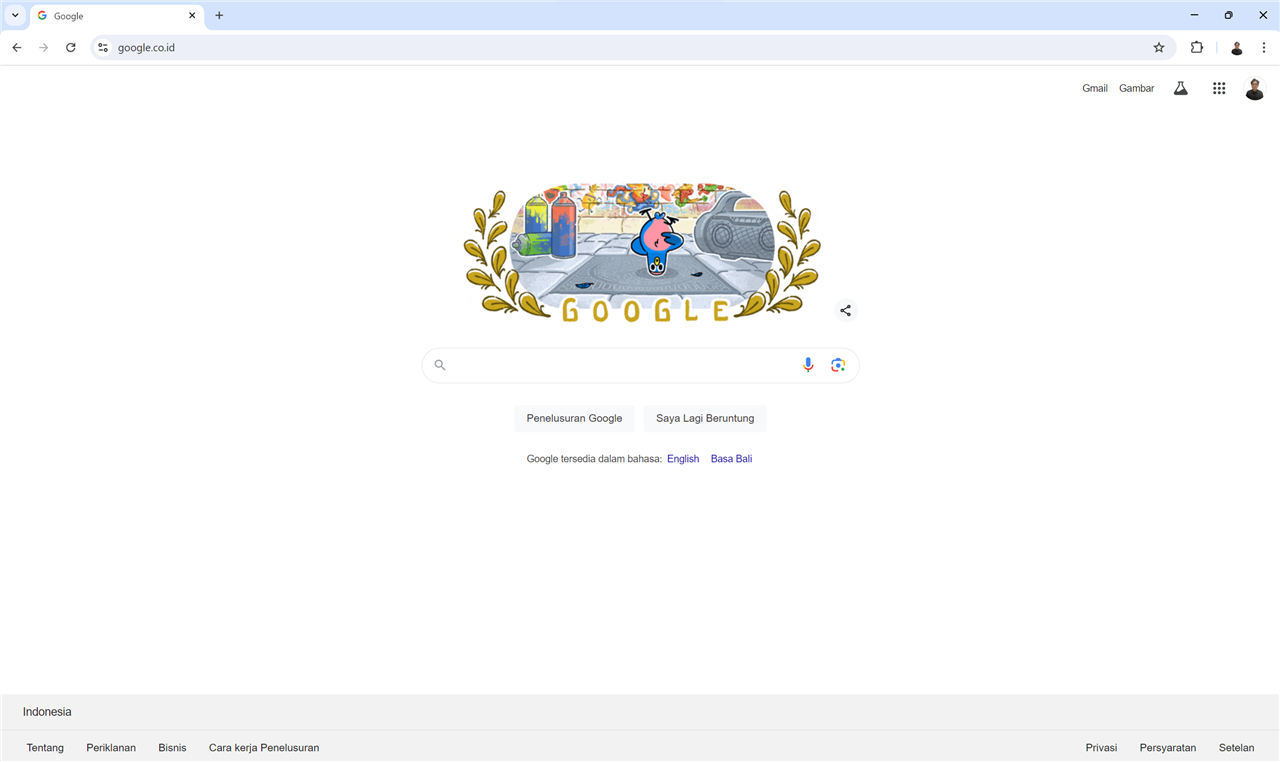
\includegraphics[width=10cm]{Gambar/bab2/website.png}
	\caption{Contoh \textit{Website}~\cite{website2024google}}
	\label{fig:contoh-website}
\end{figure}
\FloatBarrier
%
\subsection{\textit{Web Page}}
Menurut Kumar~\cite{web2018akshi}, \textit{Web page} merupakan dokumen yang ditampilkan pada \textit{web browser}. \textit{Web page} bisa bersifat statis atau dinamis. Statis berarti halaman tersebut tetap sama atau tidak berubah, sementara dinamis berarti halaman tersebut dapat berubah. Oleh karena itu, halaman web statis berisi konten yang sama setiap kali halaman dimuat, sedangkan konten halaman web dinamis dapat dihasilkan secara langsung saat dibutuhkan. Pada \textbf{\ref{fig:contoh-web-page}} merupakan contoh \textit{web page} dengan url \url{https://www.microsoft.com/id-id/microsoft-365} yang merupakan bagian satu halaman dari \textit{website} \url{https://www.microsoft.com/id-id/}.
%
\begin{figure}[!htbp]
	\centering
	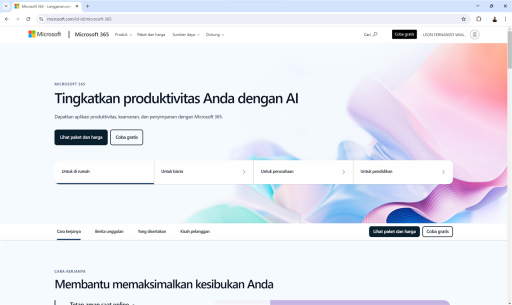
\includegraphics[width=10cm]{Gambar/bab2/web-page.png}
	\caption{Contoh \textit{Web Page}~\cite{webpage2024microsoft}}
	\label{fig:contoh-web-page}
\end{figure}
\FloatBarrier
%

\subsection{\textit{Scrum}}
Scrum adalah kerangka kerja yang dirancang untuk menerapkan prinsip-prinsip Agile dalam pengembangan. Konsep Scrum pertama kali diperkenalkan dalam artikel berjudul "The New New Product Development Game" oleh Takeuchi dan Nonaka, yang diterbitkan oleh Harvard Business Review (HBR) pada tahun 1986~\cite{magdalena2023scrum}. Menurut Hooda dkk.~\cite{hooda2023agile}, \textit{Scrum} terdiri dari 3 tahap utama yaitu \textit{outline planning}, \textit{sprint cycle}, dan \textit{project closure} yang dapat dilihat pada \textbf{\ref{fig:scrum-phases}}.
\begin{enumerate}
    \item \textit{Outline Planning}
    \\
    Pada tahap pertama, penulis akan melakukan analisis dan identifikasi kebutuhan pengguna untuk perangkat lunak. Pada tahap ini, \textit{product backlog} juga disusun, berisi daftar fitur yang dibutuhkan oleh perangkat lunak, yang diurutkan berdasarkan prioritas.
    
    \item \textit{Sprint Cycle}
    \\
    Pada tahap ini, \textit{sprint} dimulai dengan \textit{sprint planning}, yaitu proses pemilihan item dari \textit{product backlog} yang akan dikerjakan dalam setiap \textit{sprint}. Setiap \textit{sprint} berlangsung dalam iterasi pendek yang biasanya berkisar antara 1 hingga 4 minggu. Pada iterasi ini akan berfokus pada penyelesaian \textit{item} yang telah dipilih. Pada akhir setiap \textit{sprint} akan dilakukan \textit{sprint review} untuk memastikan bahwa item yang dikerjakan sudah sesuai memenuhi kriteria yang diharapkan. Siklus sprint ini akan terus berulang sampai semua item pada \textit{product backlog} terselesaikan atau proyek sudah mencapai tujuannya.

    \item \textit{Project Closure}
    \\
    Tahap terakhir adalah fase penutupan, di mana proyek diselesaikan dan ditutup secara resmi. Aktivitas yang dilakukan di tahap ini mencakup penyelesaian dokumentasi yang diperlukan, seperti panduan sistem atau manual pengguna.
\end{enumerate}
%
\begin{figure}[!htbp]
	\centering
	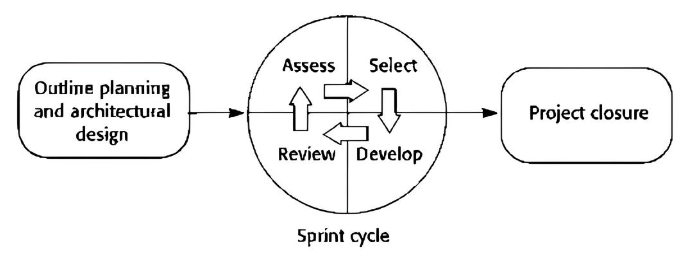
\includegraphics[width=10cm]{Gambar/bab2/scrum-methodology.png}
	\caption{\textit{Scrum Phases}~\cite{sommerville2014software}}
	\label{fig:scrum-phases}
\end{figure}
\FloatBarrier
%
Menurut Pagotto~\cite{7521555}, Metode \textit{scrum} dapat dilakukan secara individu atau sendiri yang disebut sebagai \textit{scrum solo}. \textit{Scrum Solo} memiliki karakteristik mirip dengan \textit{scrum}, seperti \textit{backlog} produk dan \textit{sprint}. Namun, \textit{scrum Solo} menggunakan \textit{sprint} satu minggu tanpa pertemuan harian. Di akhir setiap \textit{sprint}, pengembang harus menyampaikan prototipe perangkat lunak baru, dan pertemuan dengan klien atau pengguna akhir dilakukan jika diperlukan. \textit{Scrum Solo} mengintegrasikan praktik baik dari \textit{scrum} dengan fleksibilitas tambahan. Berikut ini adalah beberapa aktor proses untuk pengembangan secara individu:
\begin{enumerate}
    \item \textit{Product Owner}
    \\
    Pemilik produk yang bertanggung jawab atas visi dan arah dari produk, berinteraksi langsung dengan produk, baik sebagai individu atau sekelompok pengguna serta memastikan bahwa produk memenuhi kebutuhan pengguna dan tujuan bisnis. Mereka memberikan arahan dan keputusan penting tentang fitur dan prioritas produk.

    \item \textit{Individual Developer}
    \\
    Pengembang individu yang bertanggung jawab untuk menjalankan proses pengembangan dan membangun produk. Memiliki peran menulis kode, mengimplementasikan fitur, memperbaiki bug, dan memastikan bahwa produk berfungsi dengan baik. \textit{Individual Developer} memiliki tanggung jawab mengikuti spesifikasi dan arahan yang diberikan oleh \textit{Product Owner}, dan memastikan bahwa produk dikembangkan sesuai dengan standar dan tenggat waktu yang ditetapkan.

    \item \textit{Advisor}
    \\
     Konsultan yang memiliki pengetahuan mendalam tentang proses pengembangan. \textit{Advisor} memiliki peran Memberikan saran dan panduan tentang teknologi yang digunakan dan cakupan proyek dan bertanggung jawab menyediakan wawasan luas tentang teknologi dan metodologi yang digunakan dalam pengembangan produk, serta membantu tim dalam mengatasi tantangan teknis dan strategis.

     \item \textit{Validation Group}
     \\
     Pengguna potensial dari produk yang dihasilkan. \textit{Validation Group} memiliki peran berpartisipasi dalam proses validasi produk, dan tanggung jawab menguji produk dan memberikan umpan balik untuk memastikan bahwa produk memenuhi kebutuhan dan ekspektasi pengguna. Partisipasi mereka harus didokumentasikan dalam laporan proses.
    
\end{enumerate}

\subsection{PT Password Solusi Sistem}
Berdasarkan \textit{web} resmi MyPassword~\cite{aboutuswebsite}, MyPassword didirikan pada tahun 2009 sebagai perusahaan solusi teknologi informasi dan integrator sistem, yang menyediakan solusi infrastruktur teknologi informasi dan aplikasi bisnis, termasuk memberikan implementasi, pemeliharaan, dan layanan lainnya. Perusahaan ini dipimpin oleh dua direktur yaitu Bapak Hendriyanto Suhandi dan Bapak Julius Wendra Lea. Logo MyPassword dapat dilihat pada \textbf{\ref{fig:logo-mypassword}}.
%
\begin{figure}[!htbp]
	\centering
	
\includegraphics[width=10cm]{Gambar/bab2/logo-mypassword.png}
	\caption{Logo MyPassword~\cite{aboutuswebsite}}
	\label{fig:logo-mypassword}
\end{figure}
\FloatBarrier
%
Kantor MyPassword berlokasi di Wisma 77 \textit{Tower} 1, Lantai 15 yang dapat dilihat pada \textbf{\ref{fig:gedung-wisma-77}}, dengan alamat di Jl. Letjen S. Parman No.Kav. 77, RT.6/RW.3, Slipi, Kecamatan Palmerah, Kota Jakarta Barat, Daerah Khusus Ibukota Jakarta, 11410. MyPassword menyediakan beberapa solusi dan layanan yang ditawarkan diantaranya \textit{Modern Data Center, Modern Information System, Modern Office}, dan \textit{Modern Services}.
%
\begin{figure}[!htbp]
	\centering
	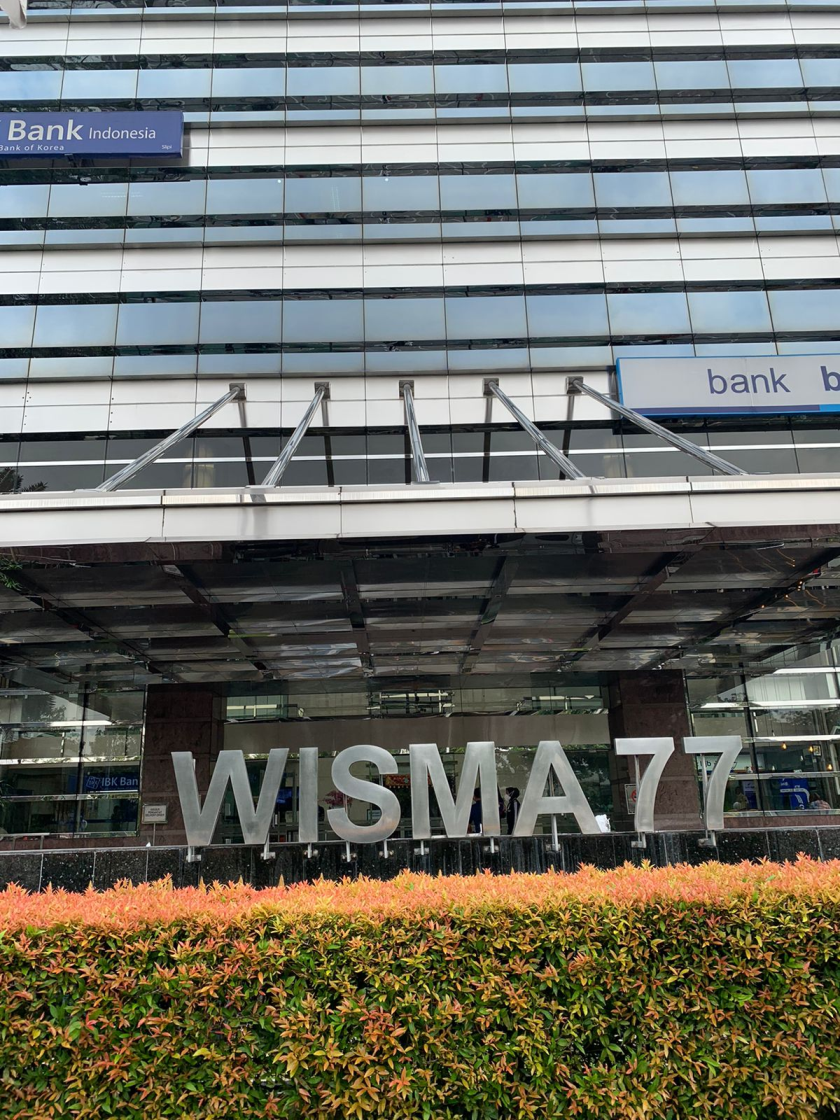
\includegraphics[width=5cm]{Gambar/bab2/gedung-wisma-77.jpeg}
	\caption{Gedung Wisma 77 \textit{Tower} 1}
	\label{fig:gedung-wisma-77}
\end{figure}
\FloatBarrier
%
MyPassword terdiri dari beberapa divisi diantaranya yaitu \textit{Business Application, Human Resources, Infrastructure, Business Support,} dan lain-lain. Jam kerja utama di kantor MyPassword yaitu Senin sampai Jumat, mulai pukul 8 pagi hingga 5 sore. Namun, untuk divisi \textit{Infrastructure} tidak semua \textit{staff} menggunakan jam kerja utama, tetapi \textit{staff Infrastructure} bekerja menggunakan jam \textit{shift} yang sudah ditentukan sehingga jam kerja mungkin akan berbeda antara satu \textit{staff} dengan \textit{staff} lainnya. Selanjutnya pada kantor MyPassword terdapat kerja lembur salah satunya divisi \textit{Infrastructure}, yang bekerja diluar jam \textit{shift} yang telah ditentukan atau bekerja pada hari libur nasional. Kerja lembur pada MyPassword juga tidak hanya dilakukan di kantor saja, tetapi juga bisa dilaksanakan di luar kantor.

Saat ini pencatatan lembur pada MyPassword sudah menggunakan aplikasi bernama "Andal". Aplikasi ini dibeli melalui pihak eksternal dengan \textit{one time payment}. Aplikasi ini dapat di-\textit{download} melalui \textit{playstore} ataupun \textit{appstore}. Pada proses bisnis aplikasi ini, \textit{Staff Infrastructure} harus melakukan presensi terlebih dahulu sebelum melakukan pengajuan lembur. Saat presensi akan dilakukan pengambilan lokasi dan foto \textit{Staff Infrastructure}. Setelah melakukan presensi maka \textit{Staff Infrastructure} dapat mengajukan formulir lembur yang mengacu pada presensi yang telah dilakukan. Jika \textit{Staff Infrastructure} lupa melakukan presensi pada hari kerja lembur maka tidak bisa melakukan pengajuan lembur sehingga \textit{Staff Infrastructure} perlu mengajukan \textit{form attendance correction} pada aplikasi. Permasalahan utama dari aplikasi yang saat ini digunakan adalah kurangnya fleksibilitas dalam penyesuaian, karena fitur-fiturnya sudah ditentukan berdasarkan layanan dari pihak ketiga. Akibatnya, ketika \textit{Staff Infrastructure} melakukan lembur lebih dari satu kali dalam sehari dalam aplikasi, perhitungan lembur harus dilakukan secara manual, yang mengakibatkan proses menjadi tidak efisien.








\section{Perancangan Proses}
Pada fase ini, akan dilakukan wawancara dengan Ibu Melissa selaku \textit{Manager Human Resource} di MyPassword. Wawancara ini akan membahas fitur-fitur yang diperlukan pada aplikasi yang akan dikembangkan dan cara pencatatan data lembur saat ini. Selain itu, wawancara ini juga akan mengeksplorasi tantangan yang dihadapi dengan menggunakan cara pencatatan lembur saat ini. \textbf{\ref{fig:wawancara-manager-human-resources}} menunjukkan sesi wawancara dengan \textit{Manager Human Resources} secara langsung di kantor MyPassword pada tanggal 26 Juli 2024 sekitar pukul 12 siang. Hasil dari wawancara dapat ditemukan pada \hyperref[sec:wawancara]{\textbf{Lampiran~II}}.

\begin{figure}[!htbp]
	\centering
	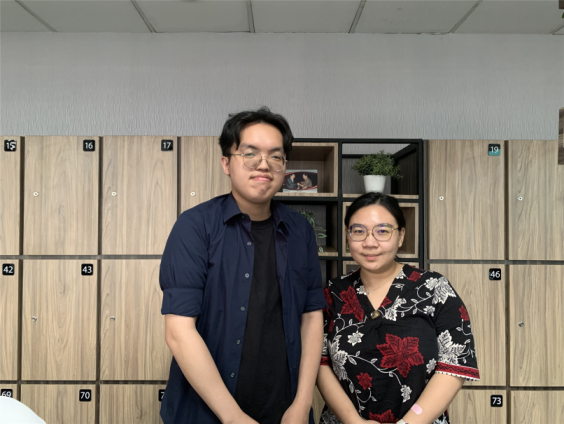
\includegraphics[width=7cm]{Gambar/bab2/dokumentasi-wawancara.jpg}
	\caption{Wawancara bersama \textit{Manager Human Resources} MyPassword}
	\label{fig:wawancara-manager-human-resources}
\end{figure}
\FloatBarrier

\subsection{Teori Umum}
\subsubsection{UML}
UML (\textit{Unified Modeling Language}) adalah bahasa grafis untuk menentukan, memvisualisasikan, membangun, dan mendokumentasikan artefak dari sistem perangkat lunak. Alat ini membantu dalam pemahaman yang lebih baik tentang perangkat lunak atau sistem atau produk yang akan dikembangkan, baik di antara pengembang maupun pelanggan~\cite{uml2022suriya}. Menurut Unhelkar~\cite{unhelkar2017software}, UML juga dapat membantu memodelkan persyaratan sistem baru dan membantu memahami proses bisnis dan aplikasi yang ada. Unhelkar juga menjelaskan terdapat beberapa jenis-jenis diagram UML:
\begin{enumerate}
    \item \textit{Use Case Diagram}
    \\ Memberikan gambaran umum tentang fungsionalitas sistem atau proses bisnis dari perspektif pengguna. Cara pengguna “menggunakan” sistem adalah titik awal untuk membuat diagram \textit{use case}.

    \item \textit{Activity Diagram}
    \\ Memodelkan aliran aktivitas normal dalam sistem dan alternatif serta pengecualian yang sangat baik digambarkan oleh diagram ini di mana saja interaksi terjadi. Khususnya, aliran dalam model \textit{use case} ke \textit{use case} di bawah diagram.

    \item \textit{Class Diagram}
    \\ Mewakili kelas, definisi mereka, hubungan, kelas dan entitas dari ruang masalah adalah entitas teknis terperinci di ruang solusi. Atribut dan operasi yang mendefinisikan kelas termasuk dalam diagram kelas ini. Hubungan dalam diagram kelas menggambarkan bagaimana kelas berinteraksi, berkolaborasi, dan mewarisi dari kelas lain.

    \item \textit{Sequence Diagram}
    \\ Memodelkan interaksi antar objek berdasarkan garis waktu mereka. Objek dapat berupa tabel, antarmuka pengguna, dan pengendali atau kelas lain juga dapat mewakili relasional untuk secara khusus ditunjukkan pada diagram ini atau mereka dapat menjadi objek anonim yang termasuk dalam suatu kelas. Urutan eksekusi pesan antar objek pada waktu runtime dimodelkan dengan baik oleh diagram ini, oleh karena itu namanya.
\end{enumerate}

\subsection{Gambar Diagram Rancangan Proses}
\subsubsection{\textit{Use Case Diagram}}
Pada rancangan \textit{use case diagram} untuk aplikasi presensi terdiri dari 3 aktor yaitu: (i) \textit{staff Infrastructure} dapat melakukan presensi masuk dan presensi keluar, serta melakukan pengajuan lembur, (ii) \textit{Manager Infrastructure} memiliki tugas untuk melakukan \textit{reject} atau \textit{penolakkan} pada data lembur yang tidak \textit{valid} dan melihat laporan lembur dan presensi (iii) \textit{Manager Human Resources} yang bertugas mengelola akun \textit{user}, melihat laporan data presensi dan lembur. \textit{Use case diagram} dari perancangan aplikasi presensi \textit{online} berbasis \textit{web} pada PT Password Solusi Sistem dapat dilihat pada \hyperref[sec:use-case-diagram-aplikasi-presensi-online]{\textbf{Lampiran~III}}.

Pada aplikasi presensi \textit{online}, \textit{staff Infrastructure} dapat melakukan \textit{login} dan \textit{logout} pada sistem, jika tidak memiliki akun dapat melakukan registrasi. \textit{Staff Infrastructure} dapat melihat jadwal jam kerja dan melakukan presensi masuk atau keluar, setelah itu mengaktifkan akses kamera dan lokasi, jika \textit{staff Infrastructure} melakukan presensi diluar jam \textit{shift} atau libur perusahaan maka sistem akan mengecek berdasarkan data \textit{shift} jam kerja \textit{staff Infrastructure} dan data hari libur perusahaan, jika syarat terpenuhi maka akan mencatat jam lembur tersebut. \textit{Staff Infrastructure} dapat melihat data riwayat presensi dan lembur, serta mengajukan \textit{form overtime request correction} jika \textit{staff Infrastructure} lupa melakukan presensi lembur. \textit{Manager Infrastructure} dan \textit{Manager Human Resource} memiliki beberapa akses yang sama seperti melakukan \textit{login} dan \textit{logout}, melihat data presensi dan lembur seluruh \textit{staff Infrastructure}, melakukan \textit{export} data presensi dan lembur dalam bentuk \textit{Microsoft Excel}, mengelola akun \textit{user} yang telah registrasi seperti mengaktifkan atau menonaktifkan, mengelola data hari libur perusahaan, mengelola \textit{shift} jam kerja \textit{staff Infrastructure} yang akan digunakan untuk pengecekkan presensi lembur. Selanjutnya perbedaan tambahan pada \textit{Manager Infrastructure} yaitu harus melakukan registrasi akun pada awal dan dapat melakukan penolakkan atau \textit{reject} pada data lembur \textit{Staff Infrastructure} yang tidak \textit{valid}.


\subsubsection{\textit{Use Case Scenario}}
\textit{Use case scenario} pada perancangan aplikasi presensi \textit{online} berbasis \textit{web} pada PT Password Solusi Sistem dapat dilihat pada \hyperref[sec:use-case-scenario-aplikasi-presensi-online]{\textbf{Lampiran~IV}}.

\subsubsection{\textit{Activity Diagram}}
\textit{Activity diagram} dari perancangan aplikasi presensi \textit{online} berbasis \textit{web} pada PT Password Solusi Sistem dapat dilihat pada \hyperref[sec:activity-diagram-aplikasi-presensi-online]{\textbf{Lampiran~V}}.

\subsubsection{\textit{Sequence Diagram}}
\textit{Sequence diagram} dari perancangan aplikasi presensi \textit{online} berbasis \textit{web} pada PT Password Solusi Sistem dapat dilihat pada \hyperref[sec:sequence-diagram-aplikasi-presensi-online]{\textbf{Lampiran~VI}}.

\subsubsection{\textit{Class Diagram}}
\textit{Class diagram} dari perancangan aplikasi presensi \textit{online} berbasis \textit{web} pada PT Password Solusi Sistem dapat dilihat pada \hyperref[sec:class-diagram-aplikasi-presensi-online]{\textbf{Lampiran~VII}}.

\section{Perancangan Basis Data}
Basis data didefinisikan sebagai kumpulan informasi yang terorganisir dan saling terkait. Tujuan utama basis data adalah untuk mengelola sejumlah besar data yang disimpan dan menyediakan informasi darinya~\cite{database2022jagdish}. Desain basis data adalah proses menghasilkan model data yang terperinci dari sebuah basis data~\cite{database2019date}. Model data \textit{entity-relationship} (E-R) adalah model data yang banyak digunakan untuk desain basis data. Model ini menyediakan representasi grafis yang nyaman untuk melihat data, hubungan, dan batasan~\cite{database2019abraham}. Menurut Conolly dan Begg~\cite{conolly2015database}, terdapat tiga fase dalam desain basis data yaitu \textit{conceptual database design, logical database design,} dan \textit{physical database design}.


\subsection{\textit{Conceptual Database Design}}
\textit{Conceptual data design} merupakan tahap untuk membangun representasi konseptual dari basis data, yang meliputi identifikasi entitas, hubungan, dan atribut penting~\cite{conolly2015database}. Perancangan \textit{conceptual data modeling} akan dilakukan dengan mengindentifikasi \textit{entity} berdasarkan hasil wawancara dengan \textit{Manager Human Resouces} di PT Password Solusi Sistem. Pada \textbf{\ref{tab:indentifikasi-entity}} menunjukkan hasil identifikasi \textit{entity} berdasarkan kebutuhan MyPassword. Pada \textbf{\ref{tab:indentifikasi-hubungan-antar-entity}} menunjukkan hubungan antar \textit{entity}. \textit{Conceptual data modeling} dalam bentuk diagram dapat dilihat pada \hyperref[sec:conceptual-database-design]{\textbf{Lampiran~VIII}}.
%%%%%%%%%%%%%%%%%%%%%%%%%%%%%%%%%%%%%%%%%%%%%%%%%%%%%%%%%%%%%%%%%
\FloatBarrier
\begin{longtable}{ |p{3cm}|p{6cm}|p{6cm}|}
\caption{Identifikasi \textit{Entity}}\label{tab:indentifikasi-entity} 
\\
\hline
\textbf{\textit{Entity}}
&\textbf{Deskripsi}
&\textbf{Kejadian / Kemunculan}
\\ 
\hline

\textit{User}
&Informasi tentang \textit{user} pada aplikasi presensi \textit{online}.
&Data \textit{user} akan dibuat ketika \textit{Staff} atau \textit{Manager Infrastructure} melakukan registrasi.
\\ 
\hline

\textit{Shift}
&Informasi tentang jenis \textit{shift} kerja.
&Data \textit{Shift} ditambahkan oleh \textit{Manager Human Resources} dan \textit{Manager Infrastructure}.
\\ 
\hline

\textit{ShiftDay}
&Informasi tentang hari dan waktu spesifik dari setiap jenis \textit{shift} yang akan digunakan untuk perhitungan lembur.
&Data \textit{ShiftDay} ditambahkan oleh \textit{Manager Human Resources} dan \textit{Manager Infrastructure}.
\\ 
\hline

\textit{Holiday}
&Informasi tentang jenis libur perusahaan.
&Data \textit{Holiday} ditambahkan oleh \textit{Manager Human Resources} dan \textit{Manager Infrastructure}.
\\ 
\hline

\textit{HolidayDay}
&Informasi tentang hari dan waktu spesifik dari setiap jenis \textit{holiday} yang akan digunakan untuk perhitungan lembur.
&Data \textit{HolidayDay} ditambahkan oleh \textit{Manager Human Resources} dan \textit{Manager Infrastructure}.
\\ 
\hline

\textit{Department}
&Informasi tentang divisi dari setiap \textit{user}.
&Data \textit{Department} ditambahkan oleh \textit{Manager Human Resources} dan \textit{Manager Infrastructure}.
\\ 
\hline

\textit{Role}
&Informasi tentang jabatan dari setiap \textit{user}.
&Data \textit{Role} ditambahkan oleh \textit{Manager Human Resources} dan \textit{Manager Infrastructure}.
\\ 
\hline

\textit{Attendance}
&Informasi tentang presensi setiap \textit{user} yang akan digunakan untuk perhitungan lembur.
&Data \textit{Attendance} akan ditambahkan ketika \textit{staff Infrastructure} melakukan presensi.
\\ 
\hline

\textit{Overtime}
&Informasi tentang lembur dari setiap \textit{staff Infrastructure}.
&Data \textit{Overtime} akan ditambahkan secara otomatis jika \textit{staff Infrastructure} melakukan presensi diluar jam \textit{shift} ataupun pada hari libur. Data \textit{Overtime} juga dapat ditambahkan secara manual oleh \textit{staff Infrastructure}.
\\ 
\hline

\textit{Session}
&Informasi tentang \textit{Session} setiap \textit{user}.
&Data \textit{Session} akan diregenerasi secara otomatis ketika \textit{user} melakukan \textit{login}.
\\
\hline

\textit{ActivityType}
&Informasi tentang jenis kerja yang dilakukan oleh \textit{staff} seperti WFO, WFH atau \textit{remote}.
&Data \textit{ActivityType} ditambahkan secara \textit{default} dengan nilai yang telah ditentukan.
\\
\hline

\textit{ActivityCategory}
&Informasi tentang kategori aktivitas pekerjaan yang dilakukan oleh \textit{staff Infrastructure} seperti instalasi dan sebagainya.
&Data \textit{ActivityCategory} ditambahkan secara \textit{default} dengan nilai yang telah ditentukan.
\\
\hline

\textit{ShiftScheduling}
&Informasi tentang penjadwalan \textit{shift} yang akan digunakan oleh setiap \textit{staff} berdasarkan jangka waktu yang diatur.
&Data \textit{ShiftScheduling} ditambahkan oleh \textit{Manager Human Resources} dan \textit{Manager Infrastructure}.
\\
\hline

\end{longtable}


%%%%%%%%%%%%%%%%%%%%%%%%%%%%%%%%%%%%%%%%%%%%%%%%%%%%%%%%%%%%%%%%%
\FloatBarrier
\begin{longtable}{ |p{2cm}|p{3cm}|p{3cm}|p{3cm}|p{3cm}|}
\caption{Identifikasi Hubungan Antar \textit{Entity}}\label{tab:indentifikasi-hubungan-antar-entity} 
\\
\hline
\textbf{\textit{Entity}}
&\textbf{\textit{Multiplicity}}
&\textbf{\textit{Relationship}}
&\textbf{\textit{Multiplicity}}
&\textbf{\textit{Entity}}
\\ 
\hline

\multirow{2}{*}{\textit{Shift}}
&1..1
&\textit{AssignedOn}
&1..*
&\textit{ShiftDay}
\\ 
\cline{2-5}
&1..1
&\textit{ShiftAssignments}
&0..*
&\textit{ShiftScheduling}
\\ 
\hline

\multirow{3}{*}{\textit{Attendance}}
&0..1
&\textit{Includes}
&0..1
&\textit{Overtime}
\\
\cline{2-5}
&1..*
&\textit{CategorizedBy}
&1..1
&\textit{ActivityType}
\\ 
\cline{2-5}
&1..*
&\textit{ClassifiedAs}
&1..1
&\textit{ActivityCategory}
\\ 
\hline

\multirow{8}{*}{\textit{User}}
&1..*
&\textit{WorksIn}
&1..1
&\textit{Department}
\\
\cline{2-5}
&1..*
&\textit{AssignedAs}
&1..1
&\textit{Role}
\\ 
\cline{2-5}
&1..1
&\textit{Records}
&0..*
&\textit{Attendance}
\\ 
\cline{2-5}
&0..1
&\textit{Requests}
&0..*
&\textit{Overtime}
\\ 
\cline{2-5}
&1..*
&\textit{ScheduledFor}
&0..1
&\textit{Shift}
\\ 
\cline{2-5}
&1..1
&\textit{Attends}
&1..1
&\textit{Session}
\\ 
\cline{2-5}
&1..*
&\textit{EntitledTo}
&0..1
&\textit{Holiday}
\\ 
\cline{2-5}
&1..1
&\textit{HasSchedules}
&0..*
&\textit{ShiftScheduling}
\\ 
\hline

\textit{Holiday}
&1..1
&\textit{AppliesOn}
&1..*
&\textit{HolidayDay}
\\ 
\hline


\end{longtable}

\subsection{\textit{Logical Database Design}}
\textit{Logical data modeling} yaitu proses menerjemahkan representasi konseptual ke dalam struktur logis basis data, yang mencakup perancangan relasi~\cite{conolly2015database}. Pada bagian \textit{logical data modeling} akan menjelaskan atribut dari setiap entitas. Diagram rancangan \textit{logical data modeling} dapat dilihat pada \hyperref[sec:logical-database-design]{\textbf{Lampiran~IX}}.

\subsection{\textit{Table Specification}}
Pada \textit{table specification} akan dijelaskan tentang tipe data dari setiap entitas, deskripsi daris setiap atribut, dan menjelaskan setiap atribut apakah memiliki status \textit{nullable, composite}, atau \textit{multivalue}. \textit{Table specification} dari \textit{database} aplikasi presensi \textit{online} pada PT Password Solusi Sistem dapat dilihat pada \hyperref[sec:table-specification]{\textbf{Lampiran~X}}.



\section{Perancangan Antar Muka Sistem}
\subsection{Mockup}
Pada perancangan antar muka sistem akan dibuat tampilan untuk aplikasi presensi \textit{online} berupa \textit{website}. Pada perancangan tampilan ini akan dibuat \textit{mockup} untuk merepresentasikan tampilan antar muka dari aplikasi. Menurut Uzayr~\cite{mastering2022sufyan}, \textit{mockup} adalah model visual dari antarmuka pengguna (UI). \textit{Mockup} memudahkan desainer untuk fokus pada visual produk. \textit{Mockup} membantu pengguna atau pemangku kepentingan untuk memahami bentuk akhir produk pada tahap awal. Saat ini, alat \textit{mockup} semakin mendapat perhatian karena membantu membangun spesifikasi UI dengan melibatkan pengguna.

\subsection{Windows Navigation Diagram}
\textit{Windows navigation diagram} akan menguraikan semua menu dalam aplikasi presensi \textit{online}. Diagram ini menyediakan peta visual yang membantu pengguna memahami struktur dan alur aplikasi presensi \textit{online}.

\subsubsection{Antar Muka Aplikasi Presensi \textit{Online}}
Aplikasi presensi \textit{online} terdapat menu \textit{login} sebagai menu pertama yang akan tampil ketika pengguna membuka url utama dari \textit{website} dan akan mengecek \textit{credential} pada pengguna. Jika sebelumnya pengguna sudah login maka akan langsung mengalihkan halaman ke menu utama. Jika tidak ada \textit{credential} maka halaman akan tetap pada menu \textit{login}. Seluruh menu dan jalur akses dari setiap menu pada aplikasi presensi \textit{online} dapat dilihat pada \textbf{\ref{fig:windows-navigation-diagram-aplikasi-presensi-online}}.
%
\begin{figure}[!htbp]
	\centering
	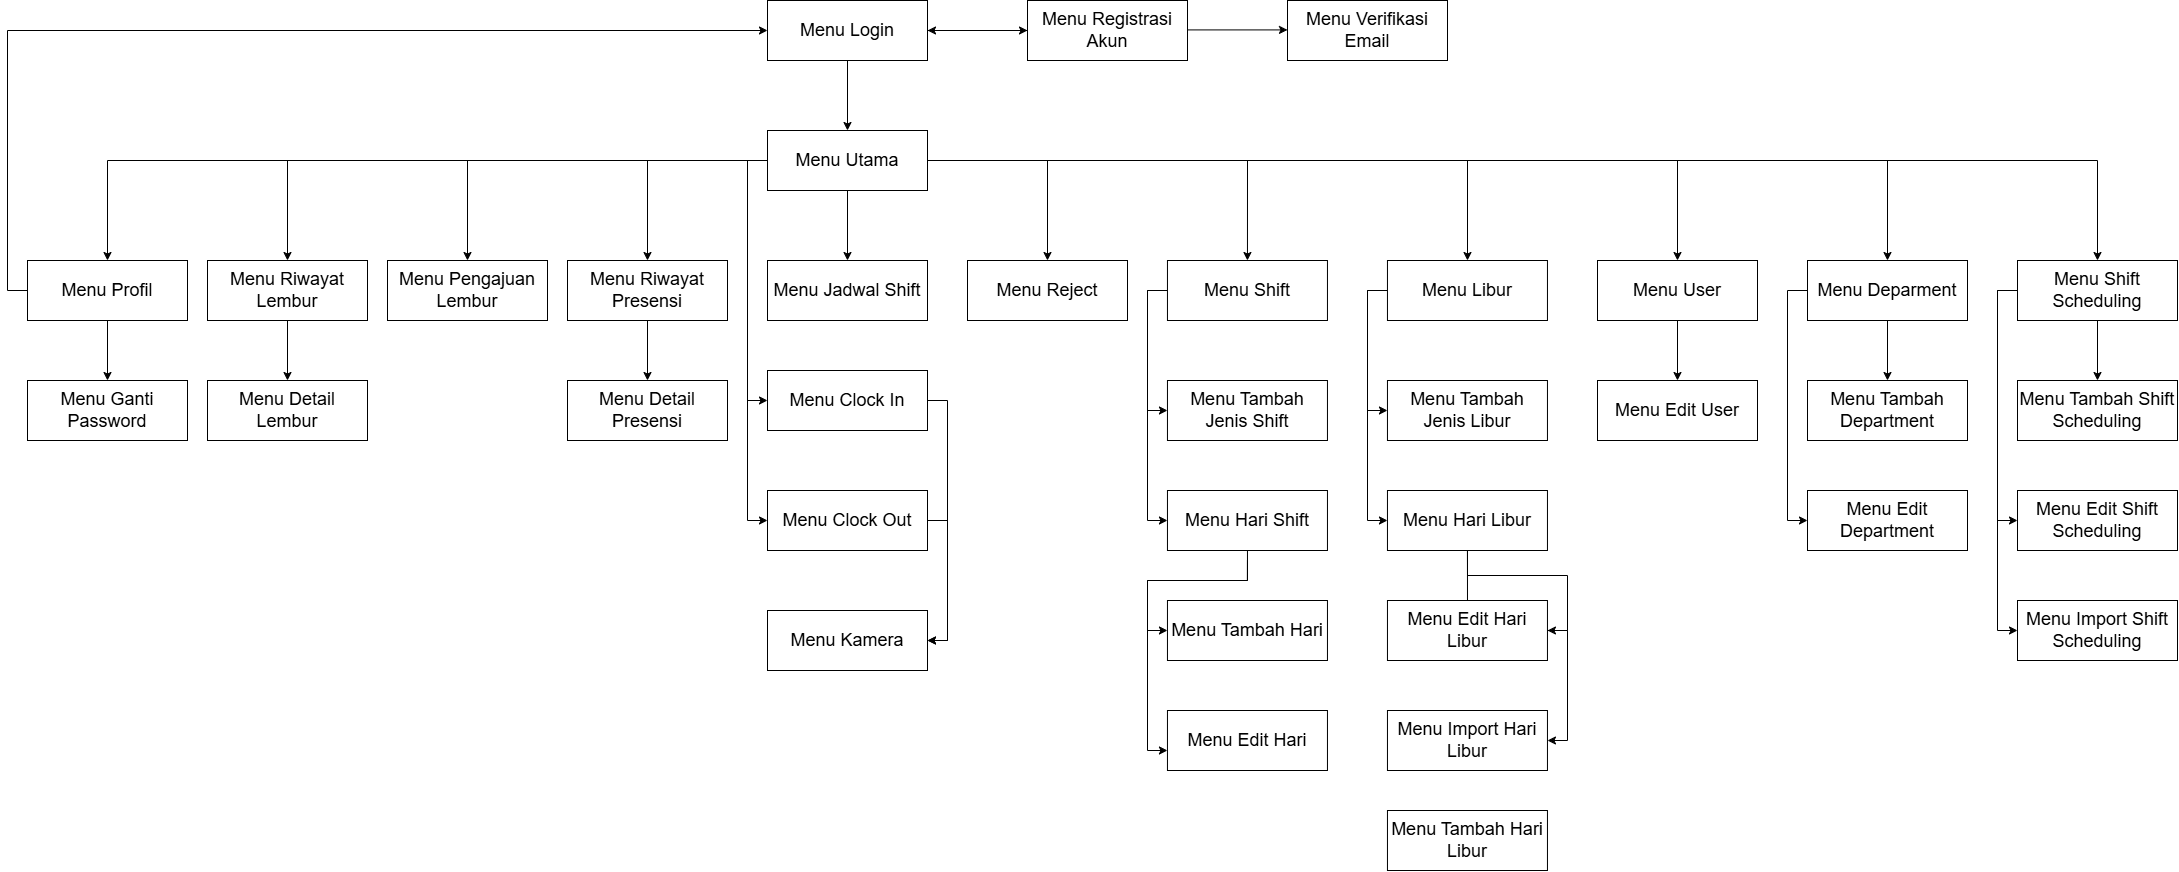
\includegraphics[width=15cm]{Gambar/bab2/windows-navigation-diagram.png}
	\caption{\textit{Windows Navigation Diagram} Aplikasi Presensi \textit{Online}}
	\label{fig:windows-navigation-diagram-aplikasi-presensi-online}
\end{figure}
\FloatBarrier

Pada aplikasi presensi \textit{online} terdiri dari 36 menu yaitu.
\begin{enumerate}
    \item Menu \textit{Utama}
    \\ Menu Utama adalah menu pertama yang muncul saat pengguna membuka aplikasi melalui tautan URL di \textit{website}. Halaman ini hanya dapat diakses ketika pengguna sudah \textit{login} sebelumnya, jika pengguna belum \textit{login} maka akan mengalihkan halaman ke Menu \textit{Login}. Menu ini juga digunakan oleh \textit{staff Infrastructure} untuk melakukan presensi. Tampilan Menu Utama dapat dilihat pada \textbf{\hyperref[sec:mockup-aplikasi-presensi-online]{Lampiran~XI}, \ref{fig:mockup-menu-utama}}.
    
    \item Menu \textit{Login}
    \\ Menu \textit{Login} merupakan menu yang berisi \textit{input form} untuk \textit{login} seluruh pengguna. Jika pengguna sudah \textit{login} sebelumnya maka halaman akan langsung dialihkan ke Menu Utama. Tampilan \textit{mockup} Menu \textit{Login} dapat dilihat pada \textbf{\hyperref[sec:mockup-aplikasi-presensi-online]{Lampiran~XI}, \ref{fig:mockup-menu-login}}.

    \item Menu Registrasi Akun
    \\ Menu Registrasi Akun merupakan halaman yang berisi \textit{input form} yang dapat digunakan oleh pengguna untuk membuat akun baru. Setelah pengguna mendaftar maka tinggal menunggu pengaktifan akun oleh \textit{manager}. Tampilan \textit{mockup} Menu Registrasi Akun dapat dilihat pada \textbf{\hyperref[sec:mockup-aplikasi-presensi-online]{Lampiran~XI}, \ref{fig:mockup-menu-registrasi-akun}}.

    \item Menu Verifikasi \textit{Email}
    \\ Menu Verifikasi \textit{Email} merupakan halaman menu yang menampilkan \textit{input form} kode OTP agar pengguna dapat melakukan verifikasi \textit{email} yang dikirimkan sistem setelah registrasi akun. Tampilan \textit{mockup} Menu Verifikasi \textit{Email} dapat dilihat pada \textbf{\hyperref[sec:mockup-aplikasi-presensi-online]{Lampiran~XI}, \ref{fig:mockup-menu-verifikasi-email}}.

    \item Menu Ganti Password
    \\ Menu Ganti Password merupakan halaman yang berisi \textit{input form} yang dapat digunakan oleh semua pengguna untuk membuat password baru akun. Tampilan \textit{mockup} Menu Ganti Password dapat dilihat pada \textbf{\hyperref[sec:mockup-aplikasi-presensi-online]{Lampiran~XI}, \ref{fig:mockup-menu-ganti-password}}.

    \item Menu Jadwal \textit{Shift}
    \\ Menu Jadwal \textit{Shift} merupakan halaman yang digunakan oleh \textit{staff Infrastructure} untuk melihat \textit{list} jadwal hari dan waktu \textit{shift} kerja. Tampilan \textit{mockup} Menu Jadwal \textit{Shift} dapat dilihat pada \textbf{\hyperref[sec:mockup-aplikasi-presensi-online]{Lampiran~XI}, \ref{fig:mockup-menu-jadwal-shift}}.

    \item Menu \textit{Clock In}
    \\ Menu \textit{Clock In} adalah halaman menu yang digunakan oleh \textit{staff Infrastructure} untuk melakukan presensi masuk. Menu ini dapat diakses ketika \textit{staff Infrastructure} menekan tombol \textit{clock in} pada Menu Utama. Pada menu ini terdapat tombol yang digunakan untuk mengambil lokasi dan tombol untuk menampilkan Menu Kamera. Tampilan \textit{mockup} Menu \textit{Clock In} dapat dilihat pada \textbf{\hyperref[sec:mockup-aplikasi-presensi-online]{Lampiran~XI}, \ref{fig:mockup-menu-clock-in}}.

    \item Menu \textit{Clock Out}
    \\ Menu \textit{Clock Out} adalah halaman menu yang digunakan oleh \textit{staff Infrastructure} untuk melakukan presensi keluar. Pada menu ini terdapat tombol untuk mengambil lokasi dan tombol untuk menampilkan Menu Kamera. Pada saat \textit{staff Infrastructure} melakukan \textit{clock out}, sistem akan mengecek data presensi saat \textit{clock in} dan \textit{clock out}, kemudian secara otomatis membuat data lembur jika presensi dilakukan diluar jam \textit{shift} atau pada hari libur. Tampilan \textit{mockup} Menu \textit{Clock Out} dapat dilihat pada \textbf{\hyperref[sec:mockup-aplikasi-presensi-online]{Lampiran~XI}, \ref{fig:mockup-menu-clock-out}}.

    \item Menu Kamera
    \\ Menu Kamera adalah menu yang digunakan oleh \textit{staff Infrastructure} untuk melakukan pengambilan foto wajah saat melakukan presensi masuk ataupun keluar. Tampilan \textit{mockup} Menu Kamera dapat dilihat pada \textbf{\hyperref[sec:mockup-aplikasi-presensi-online]{Lampiran~XI}, \ref{fig:mockup-menu-kamera}}.

    \item Menu Profil
    \\ Menu Profil adalah menu yang dapat digunakan oleh semua pengguna untuk melakukan \textit{logout} pada aplikasi dan menampilkan menu ganti password. Tampilan \textit{mockup} Menu Profil dapat dilihat pada \textbf{\hyperref[sec:mockup-aplikasi-presensi-online]{Lampiran~XI}, \ref{fig:mockup-menu-profil}}.

    \item Menu Pengajuan Lembur
    \\ Menu Pengajuan Lembur merupakan menu yang digunakan oleh \textit{staff Infrastructure} untuk membuat \textit{form} baru terkait lembur, jika \textit{staff} tersebut lupa melakukan presensi saat lembur. Tampilan \textit{mockup} Menu Pengajuan Lembur dapat dilihat pada \textbf{\hyperref[sec:mockup-aplikasi-presensi-online]{Lampiran~XI}, \ref{fig:mockup-menu-pengajuan-lembur}}.

    \item Menu Riwayat Presensi
    \\ Menu Riwayat Presensi dapat diakses oleh semua pengguna. Menu ini akan menampilkan \textit{list} data presensi yang telah dilakukan dan pengguna dapat melakukan \textit{filter} data agar dapat mencari data secara spesifik. \textit{Manager} dapat melihat seluruh presensi \textit{staff} dan melakukan \textit{export} data presensi dalam bentuk \textit{Microsoft Excel}, sedangkan \textit{staff} hanya dapat melihat presensi miliknya sendiri. Tampilan \textit{mockup} Menu Riwayat Presensi dapat dilihat pada \textbf{\hyperref[sec:mockup-aplikasi-presensi-online]{Lampiran~XI}, \ref{fig:mockup-menu-riwayat-presensi}}.

    \item Menu Detail Presensi
    \\ Menu Detail Presensi dapat diakses dengan memilih salah satu \textit{list} data presensi pada Menu Riwayat Presensi. Menu Detail Presensi menampilkan informasi lengkap dari suatu data presensi. Tampilan \textit{mockup} Menu Detail Presensi dapat dilihat pada \textbf{\hyperref[sec:mockup-aplikasi-presensi-online]{Lampiran~XI}, \ref{fig:mockup-menu-detail-presensi}}.

    \item Menu Riwayat Lembur
    \\ Menu Riwayat Lembur dapat diakses oleh semua pengguna. Menu ini akan menampilkan semua \textit{list} data lembur dan pengguna dapat melakukan \textit{filter} pada data lembur untuk mencari data yang lebih spesifik. \textit{Manager} dapat melihat semua data lembur dan melakukan \textit{export} data presensi dalam bentuk \textit{Microsoft Excel}, sedangkan \textit{staff} hanya dapat melihat data lembur miliknya sendiri. Tampilan \textit{mockup} Menu Riwayat Lembur dapat dilihat pada \textbf{\hyperref[sec:mockup-aplikasi-presensi-online]{Lampiran~XI}, \ref{fig:mockup-menu-riwayat-lembur}}.

    \item Menu Detail Lembur
    \\ Menu Detail Lembur dapat diakses dengan memilih salah satu \textit{list} data lembur pada Menu Riwayat Lembur. Menu Detail Lembur menampilkan informasi lengkap dari suatu data lembur. Tampilan \textit{mockup} Menu Detail Lembur dapat dilihat pada \textbf{\hyperref[sec:mockup-aplikasi-presensi-online]{Lampiran~XI}, \ref{fig:mockup-menu-detail-lembur}}.

    \item Menu \textit{Reject} Lembur
    \\ Menu \textit{Reject} Lembur merupakan menu yang berfungsi untuk melakukan \textit{reject} pada data lembur yang tidak \textit{valid}. \textit{Manager Infrastructure} juga dapat menggunakan fitur \textit{checkbox} untuk melakukan penolakkan lebih dari 1 data lembur. Tampilan \textit{mockup} Menu \textit{Reject} Lembur dapat dilihat pada \textbf{\hyperref[sec:mockup-aplikasi-presensi-online]{Lampiran~XI}, \ref{fig:mockup-menu-reject-lembur}}.

    \item Menu Libur
    \\ Menu Libur merupakan menu yang menampilkan \textit{list} data jenis libur pada perusahnaan. Pada menu ini juga tersedia tombol untuk membuat jenis libur baru dan mengubah data jenis libur. Data jenis libur hanya dapat dikelola oleh \textit{manager}. Tampilan \textit{mockup} Menu Libur dapat dilihat pada \textbf{\hyperref[sec:mockup-aplikasi-presensi-online]{Lampiran~XI}, \ref{fig:mockup-menu-libur}}.

    \item Menu Tambah Libur
    \\ Menu Tambah Libur merupakan menu yang dapat digunakan oleh \textit{manager} untuk membuat jenis libur baru. Tampilan \textit{mockup} Menu Tambah Libur dapat dilihat pada \textbf{\hyperref[sec:mockup-aplikasi-presensi-online]{Lampiran~XI}, \ref{fig:mockup-menu-tambah-libur}}.
    
    \item Menu Hari Libur
    \\ Menu Libur merupakan menu yang menampilkan \textit{list} data hari libur pada perusahnaan dari jenis libur yang dipilih. Pada menu ini juga tersedia tombol untuk membuat hari libur baru, mengubah data hari libur, dan melakukan \textit{import} data libur melalui API. Data hari libur hanya dapat dikelola oleh \textit{manager}. Tampilan \textit{mockup} Menu Libur dapat dilihat pada \textbf{\hyperref[sec:mockup-aplikasi-presensi-online]{Lampiran~XI}, \ref{fig:mockup-menu-hari-libur}}.

    \item Menu Tambah Hari Libur
    \\ Menu Tambah Hari libur dapat digunakan oleh \textit{manager} untuk menambah data hari libur perusahaan secara manual. Tampilan \textit{mockup} Menu Tambah Hari Libur dapat dilihat pada \textbf{\hyperref[sec:mockup-aplikasi-presensi-online]{Lampiran~XI}, \ref{fig:mockup-menu-tambah-hari-libur}}.

    \item Menu \textit{Edit} Hari Libur
    \\ Menu \textit{Edit} Hari Libur merupakan menu yang digunakan oleh \textit{manager} untuk mengubah data hari libur yang sudah ada. Tampilan \textit{mockup} Menu Hari \textit{Edit} Libur dapat dilihat pada \textbf{\hyperref[sec:mockup-aplikasi-presensi-online]{Lampiran~XI}, \ref{fig:mockup-menu-edit-hari-libur}}.

    \item Menu \textit{Import} Hari Libur
    \\ Menu \textit{Import} Hari Libur merupakan menu yang dapat digunakan oleh \textit{manager} untuk mendapatkan data libur nasional berdasarkan tahun yang dipilih melalui API, kemudian menambahkan data hari libur tersebut ke dalam jenis libur. Tampilan \textit{mockup} Menu \textit{Import} Hari Libur dapat dilihat pada \textbf{\hyperref[sec:mockup-aplikasi-presensi-online]{Lampiran~XI}, \ref{fig:mockup-menu-import-libur}}.

    \item Menu \textit{User}
    \\ Menu \textit{User} adalah menu yang menampilkan data \textit{list user} pada aplikasi presensi \textit{online}. Menu ini digunakan oleh \textit{manager} untuk mengelola data \textit{user}. Tampilan \textit{mockup} Menu \textit{User} dapat dilihat pada \textbf{\hyperref[sec:mockup-aplikasi-presensi-online]{Lampiran~XI}, \ref{fig:mockup-menu-user}}.

    \item Menu \textit{Edit User}
    \\ Menu \textit{Edit User} merupakan menu yang digunakan oleh \textit{manager} untuk mengubah data \textit{user} seperti mengantur \textit{shift} yang digunakan oleh \textit{staff} dan status aktif akun pada \textit{user}. Tampilan \textit{mockup} Menu \textit{Edit User} dapat dilihat pada \textbf{\hyperref[sec:mockup-aplikasi-presensi-online]{Lampiran~XI}, \ref{fig:mockup-menu-edit-user}}.

    \item Menu \textit{Department}
    \\ Menu \textit{Department} adalah menu yang menampilkan data \textit{list department} pada aplikasi presensi \textit{online}. Menu ini digunakan oleh \textit{manager} untuk mengelola data \textit{department}. Tampilan \textit{mockup} Menu \textit{Department} dapat dilihat pada \textbf{\hyperref[sec:mockup-aplikasi-presensi-online]{Lampiran~XI}, \ref{fig:mockup-menu-department}}.

    \item Menu Tambah \textit{Department}
    \\ Menu Tambah \textit{Department} merupakan menu yang digunakan oleh \textit{manager} untuk menambah data \textit{department} baru. Tampilan \textit{mockup} Menu Tambah \textit{Department} dapat dilihat pada \textbf{\hyperref[sec:mockup-aplikasi-presensi-online]{Lampiran~XI}, \ref{fig:mockup-menu-tambah-department}}.

    \item Menu \textit{Edit Department}
    \\ Menu \textit{Edit Department} merupakan menu yang digunakan oleh \textit{manager} untuk mengubah data \textit{department}. Tampilan \textit{mockup} Menu \textit{Edit Department} dapat dilihat pada \textbf{\hyperref[sec:mockup-aplikasi-presensi-online]{Lampiran~XI}, \ref{fig:mockup-menu-edit-department}}.

    \item Menu \textit{Shift}
    \\ Menu \textit{Shift} merupakan menu yang menampilkan \textit{list shift} yang telah dibuat. Menu ini berfungsi untuk mengelola data jenis \textit{shift} oleh \textit{manager}. Tampilan \textit{mockup} Menu \textit{Shift} dapat dilihat pada \textbf{\hyperref[sec:mockup-aplikasi-presensi-online]{Lampiran~XI}, \ref{fig:mockup-menu-shift}}. 

    \item Menu Tambah \textit{Shift}
    \\ Menu Tambah \textit{Shift} adalah menu yang dapat digunakan oleh \textit{manager} untuk menambahkan jenis \textit{shift} baru. Tampilan \textit{mockup} Menu Tambah \textit{Shift} dapat dilihat pada \textbf{\hyperref[sec:mockup-aplikasi-presensi-online]{Lampiran~XI}, \ref{fig:mockup-menu-tambah-shift}}.

    \item Menu Hari \textit{Shift}
    \\ Menu Hari \textit{Shift} merupakan menu yang berfungsi untuk mengubah nama jenis \textit{shift} dan mengelola hari dan waktu pada jenis \textit{shift} yang dipilih oleh \textit{manager}. Tampilan \textit{mockup} Menu Hari \textit{Shift} dapat dilihat pada \textbf{\hyperref[sec:mockup-aplikasi-presensi-online]{Lampiran~XI}, \ref{fig:mockup-menu-edit-shift}}.

    \item Menu Tambah Hari \textit{Shift}
    \\ Menu Tambah Hari \textit{Shift} adalah menu yang berisi \textit{input form} yang dapat digunakan oleh \textit{manager} untuk menambah hari dan waktu pada jenis \textit{shift} yang sedang di-\textit{edit}. Tampilan \textit{mockup} Menu Tambah Hari \textit{Shift} dapat dilihat pada \textbf{\hyperref[sec:mockup-aplikasi-presensi-online]{Lampiran~XI}, \ref{fig:mockup-menu-tambah-hari}}.

    \item Menu \textit{Edit} Hari \textit{Shift}
    \\ Menu \textit{Edit} Hari \textit{Shift} merupakan menu yang berisi \textit{input form} yang digunakan oleh \textit{manager} untuk mengubah hari dan waktu pada jenis \textit{shift} yang dipilih. Tampilan \textit{mockup} Menu \textit{Edit} Hari \textit{Shift} dapat dilihat pada \textbf{\hyperref[sec:mockup-aplikasi-presensi-online]{Lampiran~XI}, \ref{fig:mockup-menu-edit-hari}}.

    \item Menu \textit{Shift Scheduling}
    \\ Menu \textit{Shift Scheduling} adalah menu yang didapat digunakan oleh \textit{manager} untuk melihat \textit{list} penjadwalan \textit{shift} yang akan dipakai setiap \textit{staff} berdasarkan kurun waktu tertentu dan dapat meng-\textit{export} seluruh data penjadwalan menjadi format \textit{Excel}. Tampilan \textit{mockup} Menu \textit{Shift Scheduling} dapat dilihat pada \textbf{\hyperref[sec:mockup-aplikasi-presensi-online]{Lampiran~XI}, \ref{fig:mockup-menu-scheduling-shift}}.

    \item Menu Tambah \textit{Shift Scheduling}
    \\ Menu \textit{Shift Scheduling} adalah menu yang didapat digunakan oleh \textit{manager} untuk membuat penjadwalan \textit{shift} pada \textit{staff} dengan kurun waktu yang dipilih. Tampilan \textit{mockup} Menu Tambah \textit{Shift Scheduling} dapat dilihat pada \textbf{\hyperref[sec:mockup-aplikasi-presensi-online]{Lampiran~XI}, \ref{fig:mockup-menu-tambah-scheduling-shift}}.

    \item Menu \textit{Edit} \textit{Shift Scheduling}
    \\ Menu \textit{Edit Shift Scheduling} adalah menu yang didapat digunakan oleh \textit{manager} untuk mengubah data penjadwalan \textit{shift} pada \textit{staff} yang sudah ada. Tampilan \textit{mockup} Menu \textit{Edit} \textit{Shift Scheduling} dapat dilihat pada \textbf{\hyperref[sec:mockup-aplikasi-presensi-online]{Lampiran~XI}, \ref{fig:mockup-menu-edit-scheduling-shift}}.

    \item Menu \textit{Import} \textit{Shift Scheduling}
    \\ Menu \textit{Import Shift Scheduling} adalah menu yang didapat digunakan oleh \textit{manager} untuk meng-\textit{upload} \textit{file Excel} yang berisi \textit{list} jadwal \textit{shift} yang akan digunakan oleh setiap \textit{staff}. Tampilan \textit{mockup} Menu \textit{Import} \textit{Shift Scheduling} dapat dilihat pada \textbf{\hyperref[sec:mockup-aplikasi-presensi-online]{Lampiran~XI}, \ref{fig:mockup-menu-import-scheduling-shift}}.

    

    \end{enumerate}

\section{Perancangan Pembuatan Kode}
\label{sec:perancangan-pembuatan-kode}
\subsection{Teori}
Pada bagian teori akan menjelaskan tentang bahasa pemrograman, \textit{framework}, \textit{library}, dan basis data yang akan digunakan pada skripsi ini.

\subsubsection{HTML}
HTML adalah bahasa komputer yang dirancang khusus untuk membuat situs web yang dapat diakses oleh siapa saja tanpa memandang lokasi atau zona waktu. HTML merupakan singkatan dari \textit{Hyper Text Markup Language}. Hyper Text adalah metode yang digunakan untuk berpindah di internet~\cite{html2017micheal}. Pada dasarnya, HTML tidak lebih dari sekumpulan kode \textit{markup} yang disebut elemen yang menentukan struktur halaman web~\cite{html2024paul}. HTML memungkinkan pengembangan situs web yang dapat diakses di berbagai jenis perangkat, mulai dari PC hingga \textit{smartphone}, tanpa memerlukan instalasi \textit{plugin} yang berulang pada \textit{browser} atau pengembangan beberapa versi situs web khusus untuk perangkat seluler~\cite{theabsolute2023kevin}. Contoh kode HTML dapat dilihat pada \textbf{\ref{fig:kode-html}}.

\subsubsection{CSS}
CSS (\textit{Cascading Style Sheet}) adalah bahasa stylesheet yang diterapkan untuk menentukan bagaimana elemen HTML ditampilkan pada halaman web, termasuk desain, tata letak, dan variasi untuk perangkat dengan ukuran layar yang berbeda. CSS mengelola tata letak dari banyak situs web secara bersamaan~\cite{html2023sufyan}. CSS adalah alat yang unik dalam pengembangan perangkat lunak. Meskipun bukan bahasa pemrograman dalam arti tradisional, CSS tetap membutuhkan pemikiran abstrak~\cite{css2023keith}. CSS memberikan fleksibilitas dalam desain web, memungkinkan konsistensi di seluruh situs sekaligus memudahkan perubahan pada halaman individu atau bagian tertentu sesuai kebutuhan~\cite{mastering2023sufyan}. Contoh kode CSS dapat dilihat pada \textbf{\ref{fig:kode-css}}.

%%%%%%%%%%%%%%%%%%%%%%%%%%%%%%%%%%%%%%%%%%%%%%%%
\begin{figure}[!htbp]
	\centering
	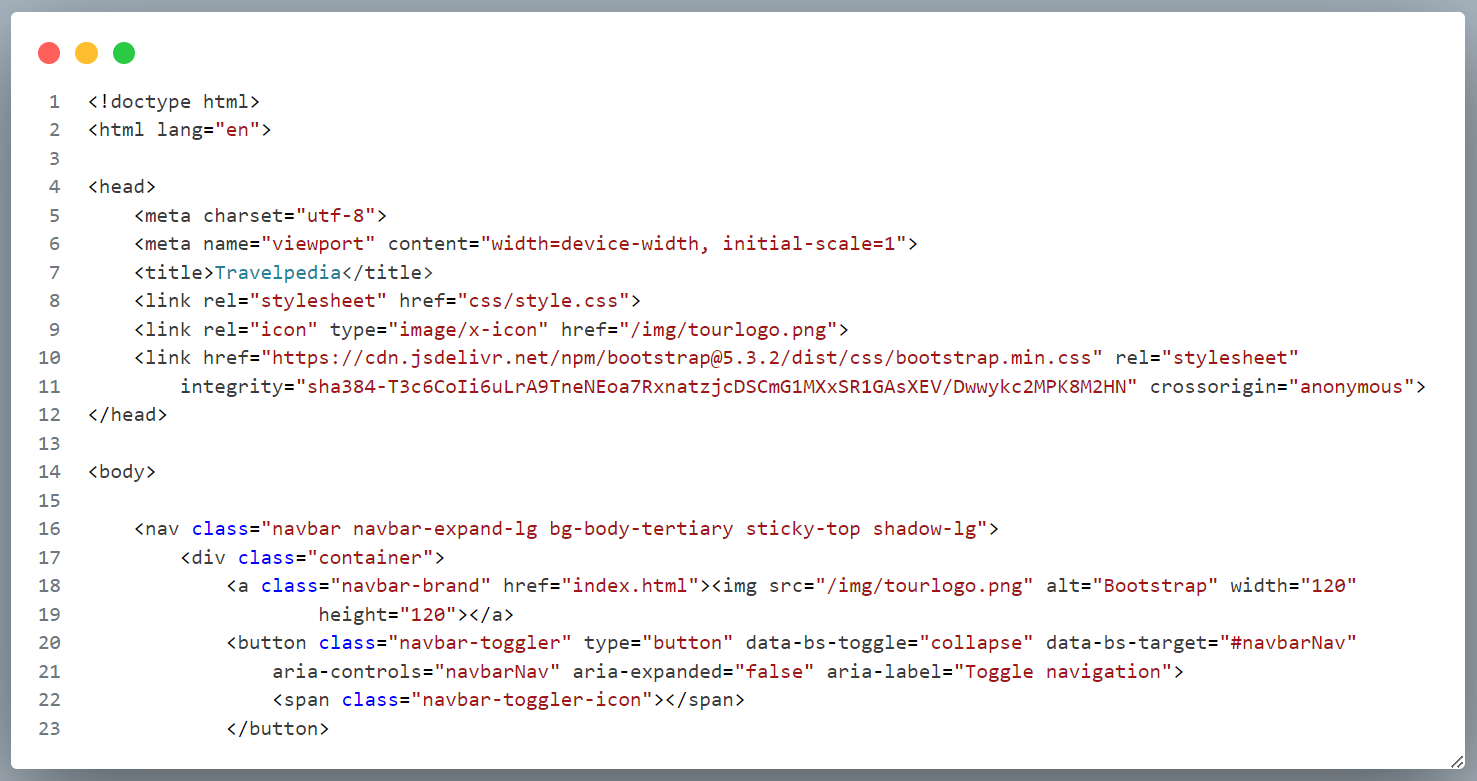
\includegraphics[width=16cm]{Gambar/bab2/html.png}
	\caption{Kode HTML}
	\label{fig:kode-html}
\end{figure}
\FloatBarrier

%%%%%%%%%%%%%%%%%%%%%%%%%%%%%%%%%%%%%%%%%%%%%%%%
\begin{figure}[!htbp]
	\centering
	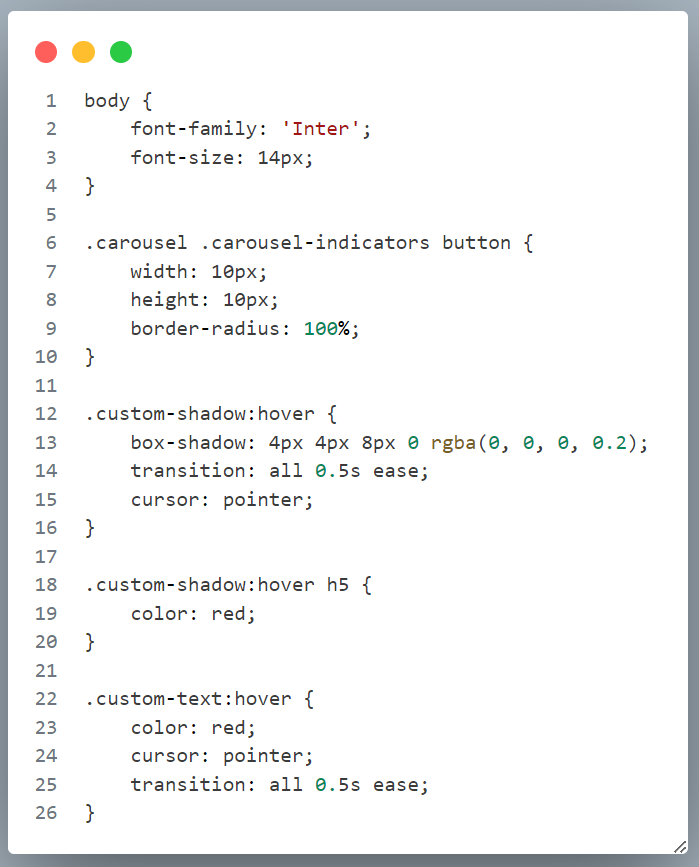
\includegraphics[width=7cm]{Gambar/bab2/css.png}
	\caption{Kode CSS}
	\label{fig:kode-css}
\end{figure}
\FloatBarrier

\subsubsection{JavaScript}
JavaScript adalah bahasa pemrograman dinamis yang terutama digunakan untuk membuat elemen interaktif pada halaman web. JavaScript memungkinkan pengembang untuk menambahkan berbagai fungsionalitas ke halaman web, termasuk validasi formulir, peta interaktif, grafik animasi, dan tata letak halaman web yang kompleks. Tidak seperti banyak bahasa pemrograman lainnya, JavaScript dieksekusi di browser pengguna (\textit{client-side})~\cite{basics2024unknown}. Dalam JavaScript, terdapat teknik bernama ajax yang berfungsi untuk membuat permintaan ke server untuk data tambahan tanpa perlu memuat ulang halaman web, yang menghasilkan pengalaman pengguna yang lebih baik~\cite{professional2023matt}. HTML DOM (\textit{Document Object Model}) merepresentasikan segala sesuatu di halaman HTML sebagai sebuah pohon Node, termasuk komentar HTML dan setiap spasi kosong. Semua elemen dalam DOM dapat diakses oleh JavaScript dan bisa diubah, dan setiap perubahan yang dilakukan oleh JavaScript akan langsung tercermin di halaman yang ditampilkan kepada pengguna~\cite{quick2023david}. Contoh kode JavaScript dapat dilihat pada \textbf{\ref{fig:kode-javascript}}.
%%%%%%%%%%%%%%%%%%%%%%%%%%%%%%%%%%%%%%%%%%%%%%%%
\begin{figure}[!htbp]
	\centering
	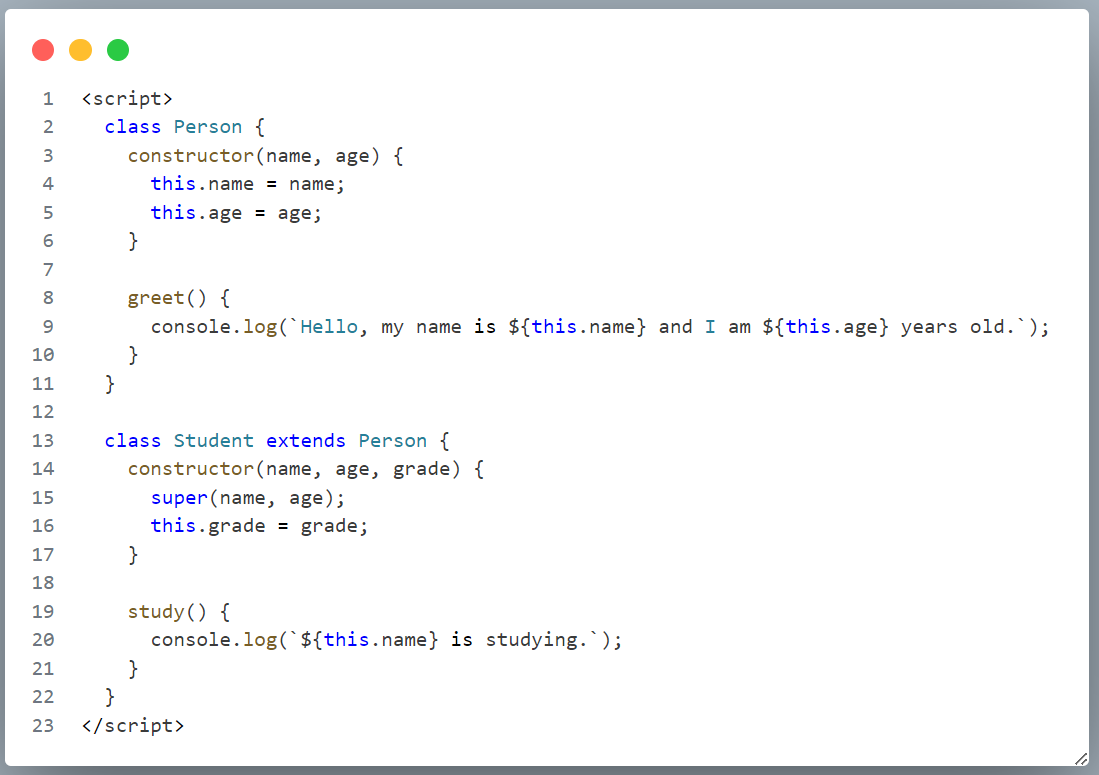
\includegraphics[width=14cm]{Gambar/bab2/javascript.png}
	\caption{Kode JavaScript}
	\label{fig:kode-javascript}
\end{figure}
\FloatBarrier

\subsubsection{PHP}
PHP adalah bahasa pemrograman yang berjalan di sisi server, berbeda dengan JavaScript yang merupakan bahasa pemrograman sisi klien~\cite{php2022tom}. PHP mendukung berbagai \textit{database} populer, seperti MySQL, PostgreSQL, Oracle, Sybase, Informix, dan \textit{Microsoft} SQL \textit{Server}, yang membuatnya fleksibel untuk berbagai kebutuhan pengembangan aplikasi web~\cite{php2022sufyan}. Contoh kode PHP dapat dilihat pada \textbf{\ref{fig:kode-php}}.
%%%%%%%%%%%%%%%%%%%%%%%%%%%%%%%%%%%%%%%%%%%%%%%%
\begin{figure}[!htbp]
	\centering
	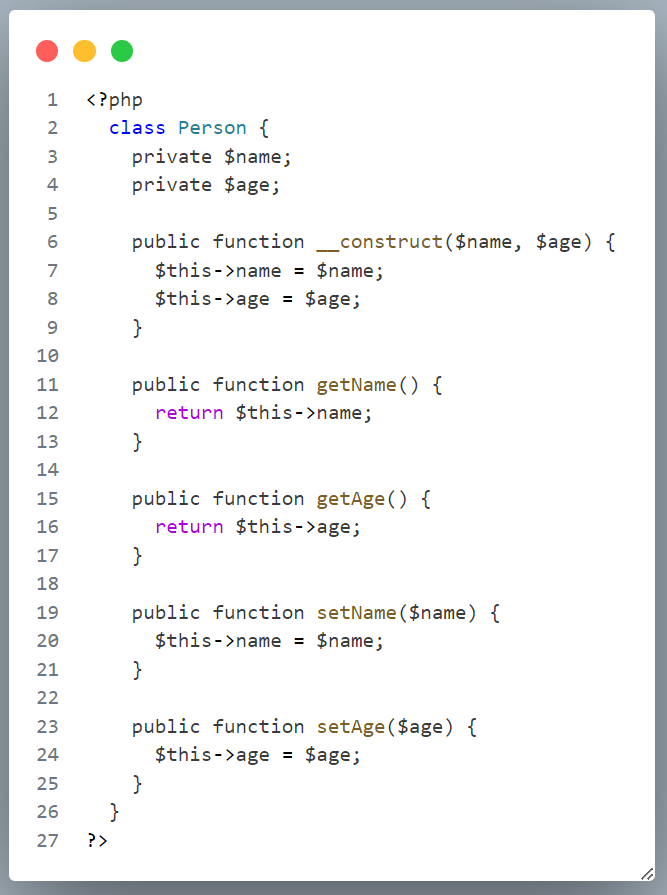
\includegraphics[width=8cm]{Gambar/bab2/php.png}
	\caption{Kode PHP}
	\label{fig:kode-php}
\end{figure}
\FloatBarrier

\subsubsection{JQuery}
jQuery bertujuan untuk menyederhanakan dan meningkatkan efisiensi penggunaan JavaScript dengan membuatnya lebih cepat, mudah, ringkas, dan menarik. \textit{Library} ini memungkinkan pengembang untuk membuat situs web yang lebih dinamis dan interaktif dengan memanfaatkan berbagai metode bawaan yang telah ditentukan. Dengan jQuery, banyak fungsi JavaScript yang biasa digunakan, yang biasanya memerlukan beberapa baris kode, dapat diakses dan dijalankan hanya dengan satu baris kode, sehingga mempercepat dan mempermudah proses pengembangan~\cite{masteringjquery2023sufyan}. Dokumentasi JQuery dapat diakses melalui \url{https://api.jquery.com/}. Contoh kode JQuery dapat dilihat pada \textbf{\ref{fig:kode-jquery}}.
%%%%%%%%%%%%%%%%%%%%%%%%%%%%%%%%%%%%%%%%%%%%%%%%
\begin{figure}[!htbp]
	\centering
	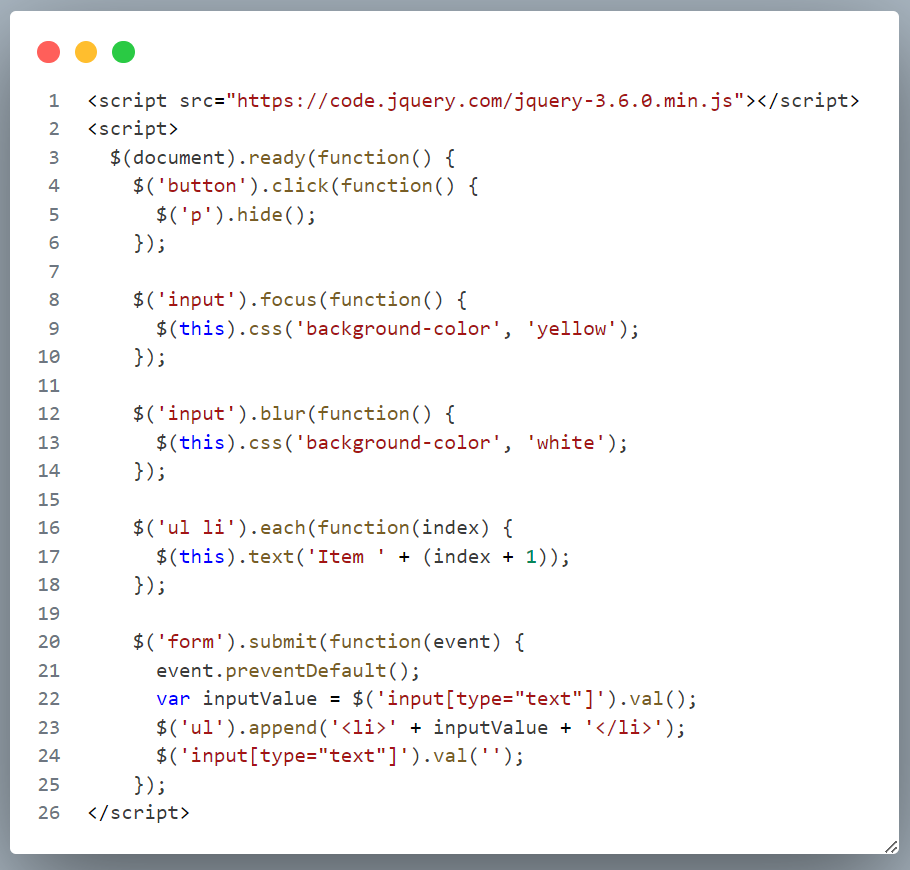
\includegraphics[width=10cm]{Gambar/bab2/jquery.png}
	\caption{Kode JQuery}
	\label{fig:kode-jquery}
\end{figure}
\FloatBarrier

\subsubsection{Laravel}
Laravel adalah \textit{framework} PHP yang gratis dan sumber terbuka yang menyediakan seperangkat alat dan sumber daya untuk membangun aplikasi web PHP modern. Laravel menyediakan sintaks yang elegan, fitur bawaan, dan berbagai paket serta ekstensi yang kompatibel. Saat pengembangan Laravel secara \textit{local}, membutuhkan XAMPP dan \textit{composer}. XAMPP adalah lingkungan pengembangan PHP yang paling populer. XAMPP adalah distribusi Apache yang gratis dan mudah diinstal yang mencakup MySQL, PHP, dan Perl. Composer adalah alat untuk mengelola ketergantungan dalam pengembangan PHP. Alat ini memudahkan mengelola \textit{libraries} yang dibutuhkan saat pengembangan proyek~\cite{practical2022daniel}. \textit{Framework} ini menyederhanakan berbagai tugas umum dalam pengembangan web, seperti interaksi dengan \textit{database}, autentikasi, antrian, pengiriman \textit{email}, dan \textit{caching}, berkat komponen-komponennya yang terintegrasi~\cite{laravel2023matt}. Dokumentasi Laravel dapat diakses melalui \url{https://laravel.com/docs/10.x/installation}. Kode \textit{command line} untuk instalasi \textit{framework} Laravel dengan composer dapat dilihat pada \textbf{\ref{fig:install-laravel}}. 
%%%%%%%%%%%%%%%%%%%%%%%%%%%%%%%%%%%%%%%%%%%%%%%%
\begin{figure}[!htbp]
	\centering
	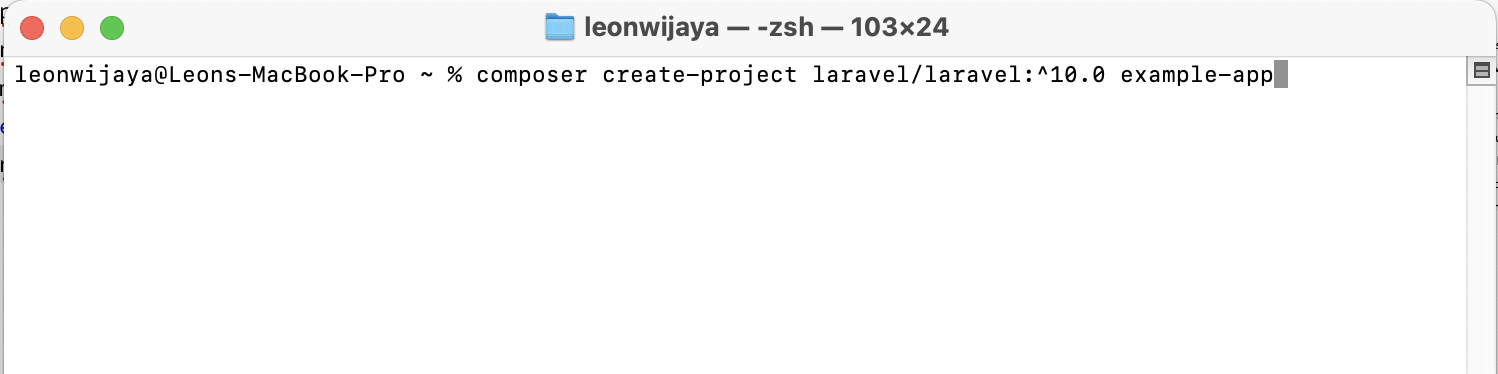
\includegraphics[width=8cm]{Gambar/bab2/install-laravel.png}
	\caption{Kode \textit{Command Line} Instalasi \textit{Framework} Laravel dengan Composer}
	\label{fig:install-laravel}
\end{figure}
\FloatBarrier

\subsubsection{TensorFlow}
TensorFlow adalah \textit{framework machine learning} yang memungkinkan pengembang untuk mengembangkan solusi \textit{machine learning} dengan cepat untuk berbagai kasus penggunaan khusus yang dapat memanfaatkan  \textit{machine learning}~\cite{thushan2022tensorflow}. TensorFlow dibuat di Google dan mendukung banyak aplikasi  \textit{machine learning} skala besar~\cite{hands2022aurelien}. TensorFlow memungkinkan pengembang untuk mendefinisikan dan melatih berbagai jenis model \textit{machine learning}, termasuk \textit{deep neural networks}, untuk berbagai tugas seperti \textit{classification}, \textit{regression}, \textit{clustering}, dan lain-lain~\cite{mastering2024hasan}. Pada aplikasi ini, model \textit{simple face detection (BlazeFace)} akan digunakan untuk mendeteksi wajah pada gambar selama pengambilan foto saat melakukan presensi. Dokumentasi TensorFlow dapat dilihat melalui \url{https://www.tensorflow.org/js/models}.

\subsubsection{Tailwind CSS}
Tailwind adalah sekumpulan kelas utilitas dasar yang dapat digunakan seperti blok penyusun untuk menciptakan berbagai desain yang kita inginkan. \textit{Framework} yang berfokus pada utilitas ini mencakup properti CSS yang paling penting, tetapi juga mudah diperluas dengan berbagai cara~\cite{tailwind2022ivaylo}. Tailwind CSS memiliki beberapa keunggulan, termasuk kemudahan dalam membuat prototipe, iterasi, dan kustomisasi tampilan, serta menyediakan \textit{modifier} untuk perilaku khusus. Selain itu, penggunaan Tailwind mengurangi penulisan CSS karena desain lebih banyak berasal dari komposisi \textit{utility}-nya~\cite{modern2022noel}. Dokumentasi Tailwind CSS dapat diakses melalui \url{https://tailwindcss.com/docs/installation}. Penulis menggunakan Tailwind CSS sebagai alat untuk mempermudah proses \textit{styling} pada tampilan aplikasi.


\subsubsection{Flowbite}
Flowbite merupakan \textit{library} komponen UI \textit{open source} yang dikembangakan dengan \textit{framework} Tailwind CSS yang berfokus pada pendekatan \textit{utility first}. \textit{Library} ini menyediakan berbagai komponen penting yang sering digunakan dalam pengembangan web, seperti tombol, \textit{dropdown}, \textit{navigation bar}, dan \textit{modal}~\cite{introduction2024flowbite}. Dokumentasi Flowbite dapat diakses melalui \url{https://flowbite.com/docs/getting-started/introduction/}. Penulis menggunakan Flowbite untuk mempercepat proses pembuata antarmuka pengguna (UI) karena terdapat komponen siap pakai.

\subsubsection{MySQL}
MySQL adalah sistem manajemen basis data relasional (RDBMS) sumber terbuka yang dikembangkan oleh perusahaan Swedia, MySQL AB. Perusahaan ini didirikan oleh David Axmark, Allan Larsson, dan Michael Widenius, dengan pengembangan awal MySQL dimulai oleh Widenius dan Axmark pada tahun 1994~\cite{masteringmysql2022sufyan}. MySQL banyak digunakan oleh beberapa organisasi dan pengembang karena beberapa alasan utama diantaranya yaitu bersifat open-source dan biasanya gratis, kinerja yang sangat cepat, mudah di-\textit{install} dan digunakan~\cite{mysql2023ben}.

\chapter{\vspace{2ex}PEMBUATAN DAN IMPLEMENTASI}

\section{Tata Laksana Program yang dibuat}
Pada bagian tatak laksana program yang dibuat akan dijelaskan beberapa langkah-langkah yang dilakukan dalam proses pembuatan program yaitu sebagai berikut.

\subsection{Persiapan lingkungan Pengembangan Aplikasi}
Pengembangan aplikasi presensi \textit{online} akan menggunakan \textit{framework} Laravel. \textit{framework} ini merupakan \textit{framework backend}, namun \textit{framework} ini menyediakan \textit{blade templating} agar dapat mengembangkan sisi \textit{frontend}. \textit{Framework} ini menggunakan konsep MVC (\textit{Model-View-Controller}) yang memisahkan logika aplikasi menjadi tiga bagian utama, sehingga memudahkan pengelolaan dan pengembangan aplikasi dengan lebih terstruktur. Untuk membuat proyek Laravel baru, dibutuhkan PHP dengan versi 8 keatas. Penulis melakukan instalasi XAMPP karena didalamnya sudah termasuk PHP, \textit{apache}, dan basis data MySQL. Instalasi dapat dilakukan melalui tautan \url{https://www.apachefriends.org/download.html}. \textbf{~\ref{fig:tampilan-XAMPP}} menunjukkan tampilan XAMPP setelah selesai instalasi.
 %
    \begin{figure}[!htbp]
    	\centering
    	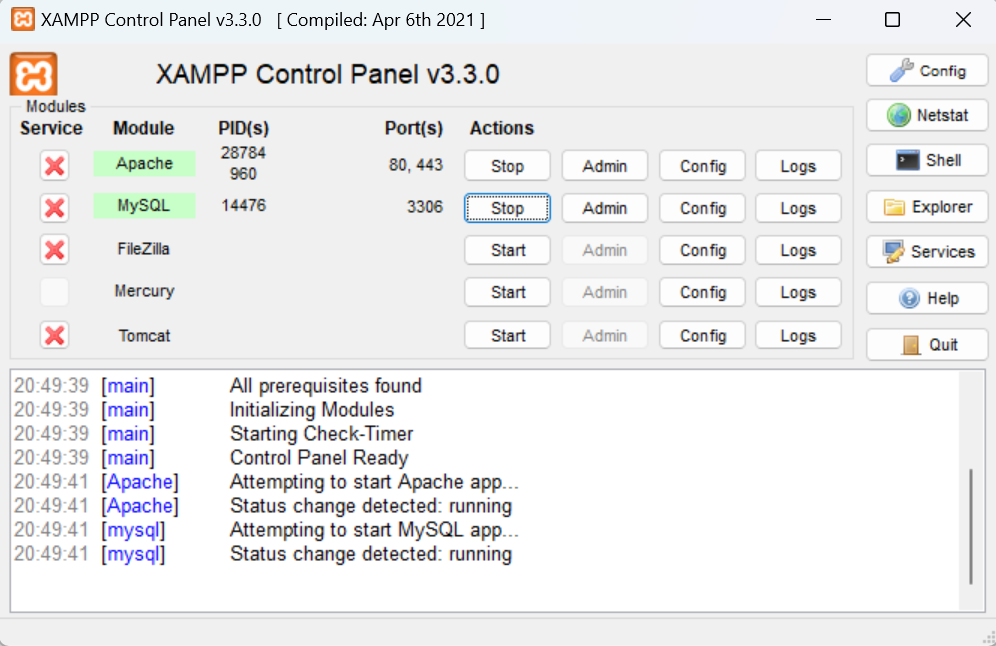
\includegraphics[width=10cm]{Gambar/bab3/start-xampp.png}
    	\caption{Tampilan XAMPP}
    	\label{fig:tampilan-XAMPP}
    \end{figure}
    \FloatBarrier
    %
Setelah itu, dibutuhkan juga Composer untuk \textit{dependency manager} untuk mengelola \textit{package} dan dependensi lainnya. Instalasi Composer dapat dilakukan melalui tautan \url{https://getcomposer.org/download/}. Jika semua sudah ter-\textit{install}, jalankan \textit{command line} yang dapat dilihat pada \textbf{~\ref{fig:command-line-create-laravel}}. 
%
    \begin{figure}[!htbp]
    	\centering
    	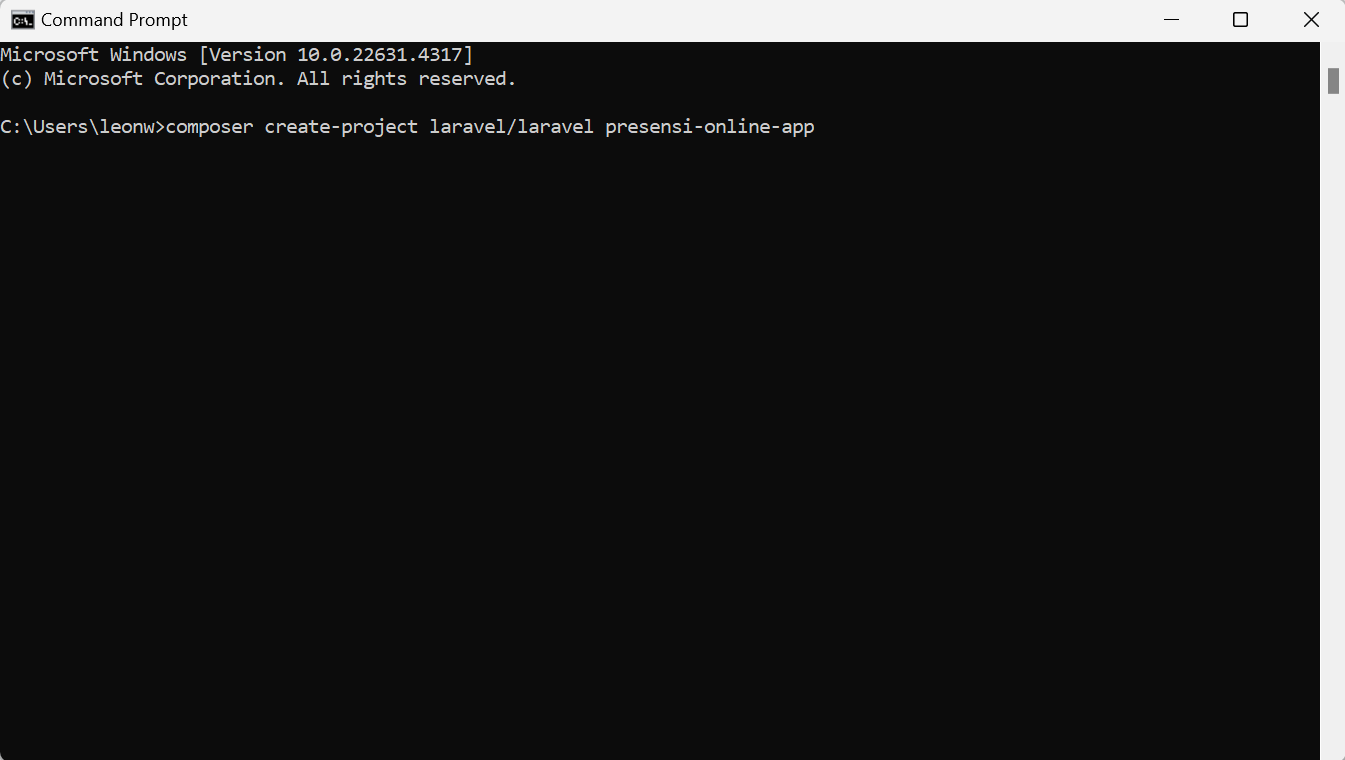
\includegraphics[width=10cm]{Gambar/bab3/command-line-create-laravel.png}
    	\caption{Tampilan \textit{Command Line} Instalasi Laravel}
    	\label{fig:command-line-create-laravel}
    \end{figure}
    \FloatBarrier
    %
Pada pengembangan aplikasi presensi \textit{online} akan menggunakan \textit{Visual Studio Code} sebagai \textit{code editor} yang dapat di-\textit{download} melalui tautan \url{https://code.visualstudio.com/}. \textbf{~\ref{fig:tampilan-laravel-vscode}} menunjukkan tampilan struktur kode Laravel yang dibuka melalui \textit{Visual Studio Code}.
%
    \begin{figure}[!htbp]
    	\centering
    	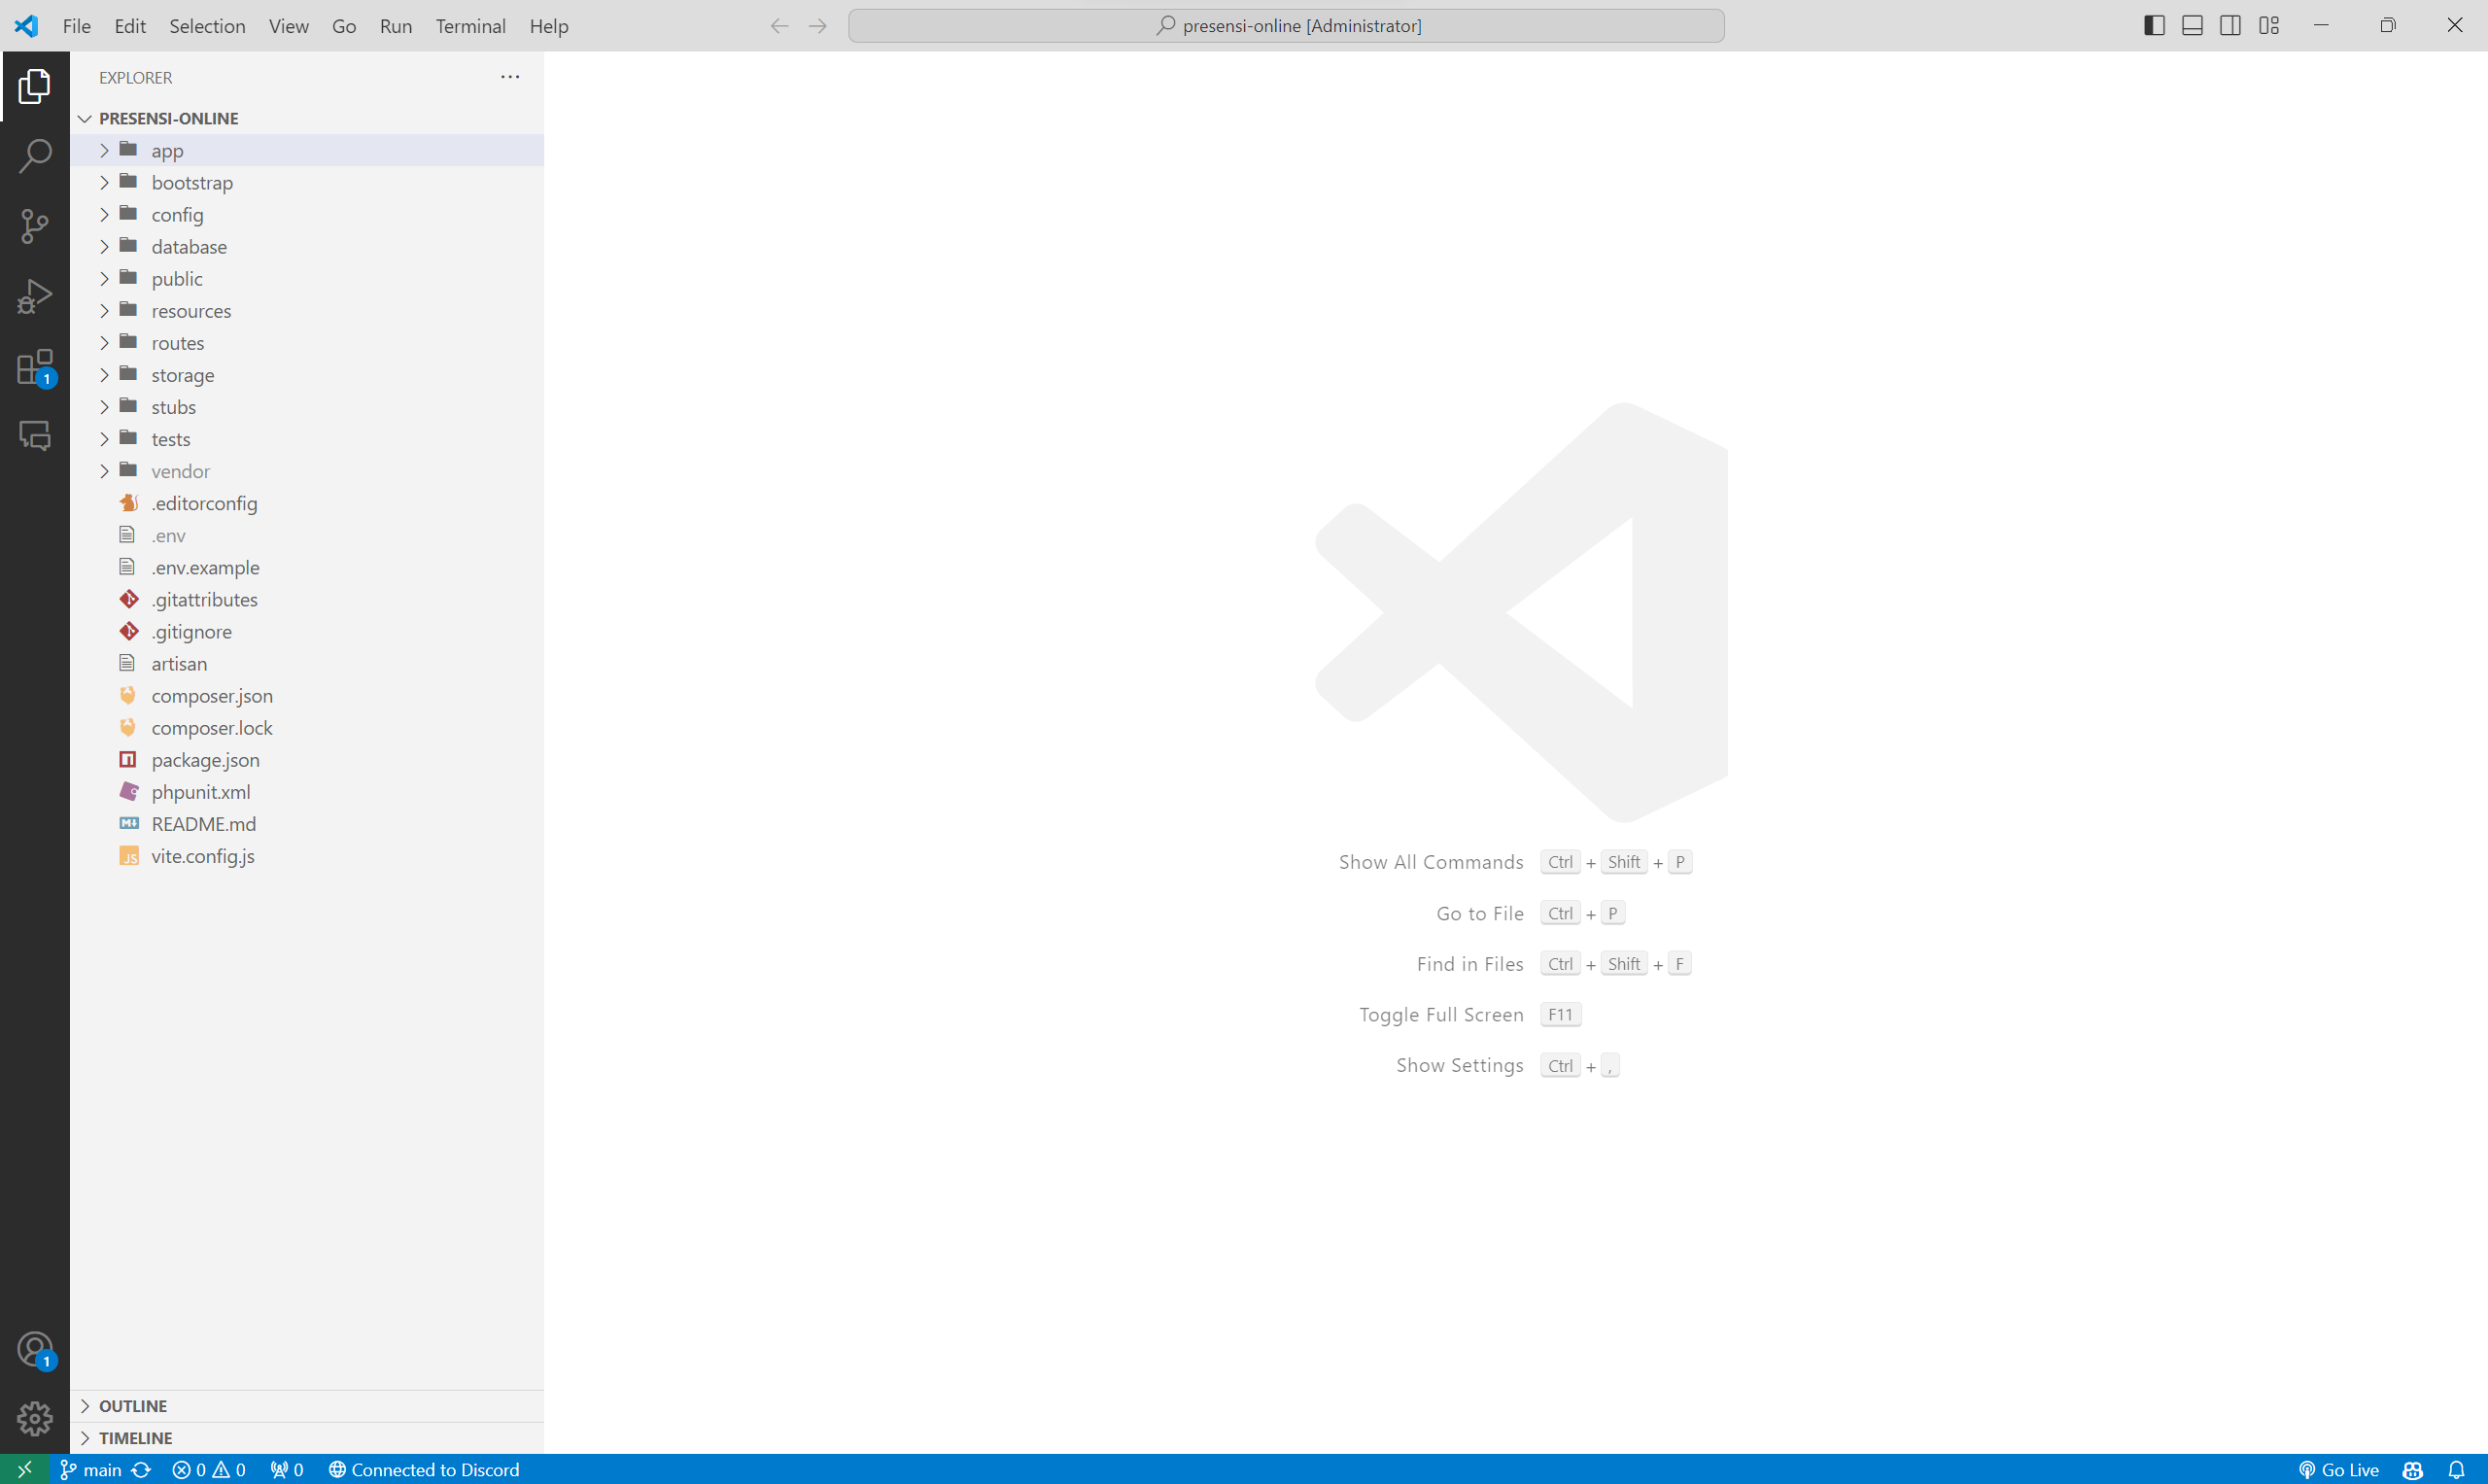
\includegraphics[width=16cm]{Gambar/bab3/code-editor-laravel.png}
    	\caption{Tampilan Struktur Kode Laravel Pada \textit{Visual Studio Code}}
    	\label{fig:tampilan-laravel-vscode}
    \end{figure}
    \FloatBarrier
    %

\subsection{Membuat \textit{Database}}
\textit{Database} yang akan digunakan pada aplikasi ini adalah MySQL. Instalasi MySQL sudah dilakukan bersamaan dengan instalasi XAMPP yang sudah dilakukan pada tahap sebelumnya. Selanjutnya, untuk pembuatan \textit{database} akan menggunakan fitur dari Laravel yaitu \textit{migration}. Sebelumnya, perlu dilakukan konfigurasi \textit{file} .env pada struktur folder Laravel untuk mengatur konfigurasi aplikasi termasuk basis data. \textbf{~\ref{fig:tampilan-file-env}} menampilkan \textit{file} .env yang sudah dikonfigurasi. Laravel menyediakan fitur \textit{migration} untuk membuat tabel pada basis data menggunakan \textit{command line}. \textit{Command line} "php artisan make:model Department -m" merupakan salah satu contoh pembuatan \textit{Model} bersamaan dengan \textit{migration} pada tabel \textit{Department}. Setelah itu mengatur isi kolom yang ingin ditambahkan pada tabel. \textbf{~\ref{fig:tampilan-migration-department}} menunjukkan isi \textit{file migration} yang telah diatur isi kolomnya. Kemudian, jalankan \textit{command line} "php artisan migrate" untuk membuat tabel beserta isi kolomnya. Laravel juga menyediakan fitur \textit{seeder} yang dapat digunakan untuk mengisi baris tabel \textit{Department} dengan menjalankan \textit{command line} "php artisan make:seeder DepartmentSeeder". \textbf{~\ref{fig:tampilan-seeder-department}} menunjukkan isi \textit{file} DepartmentSeeder yang sudah diatur nilainya. Kemudian, jalankan \textit{command line} "php artisan db:seed -class=DepartmentSeeder" untuk memasukkan nilainya ke dalam tabel.
%
    \begin{figure}[!htbp]
    	\centering
    	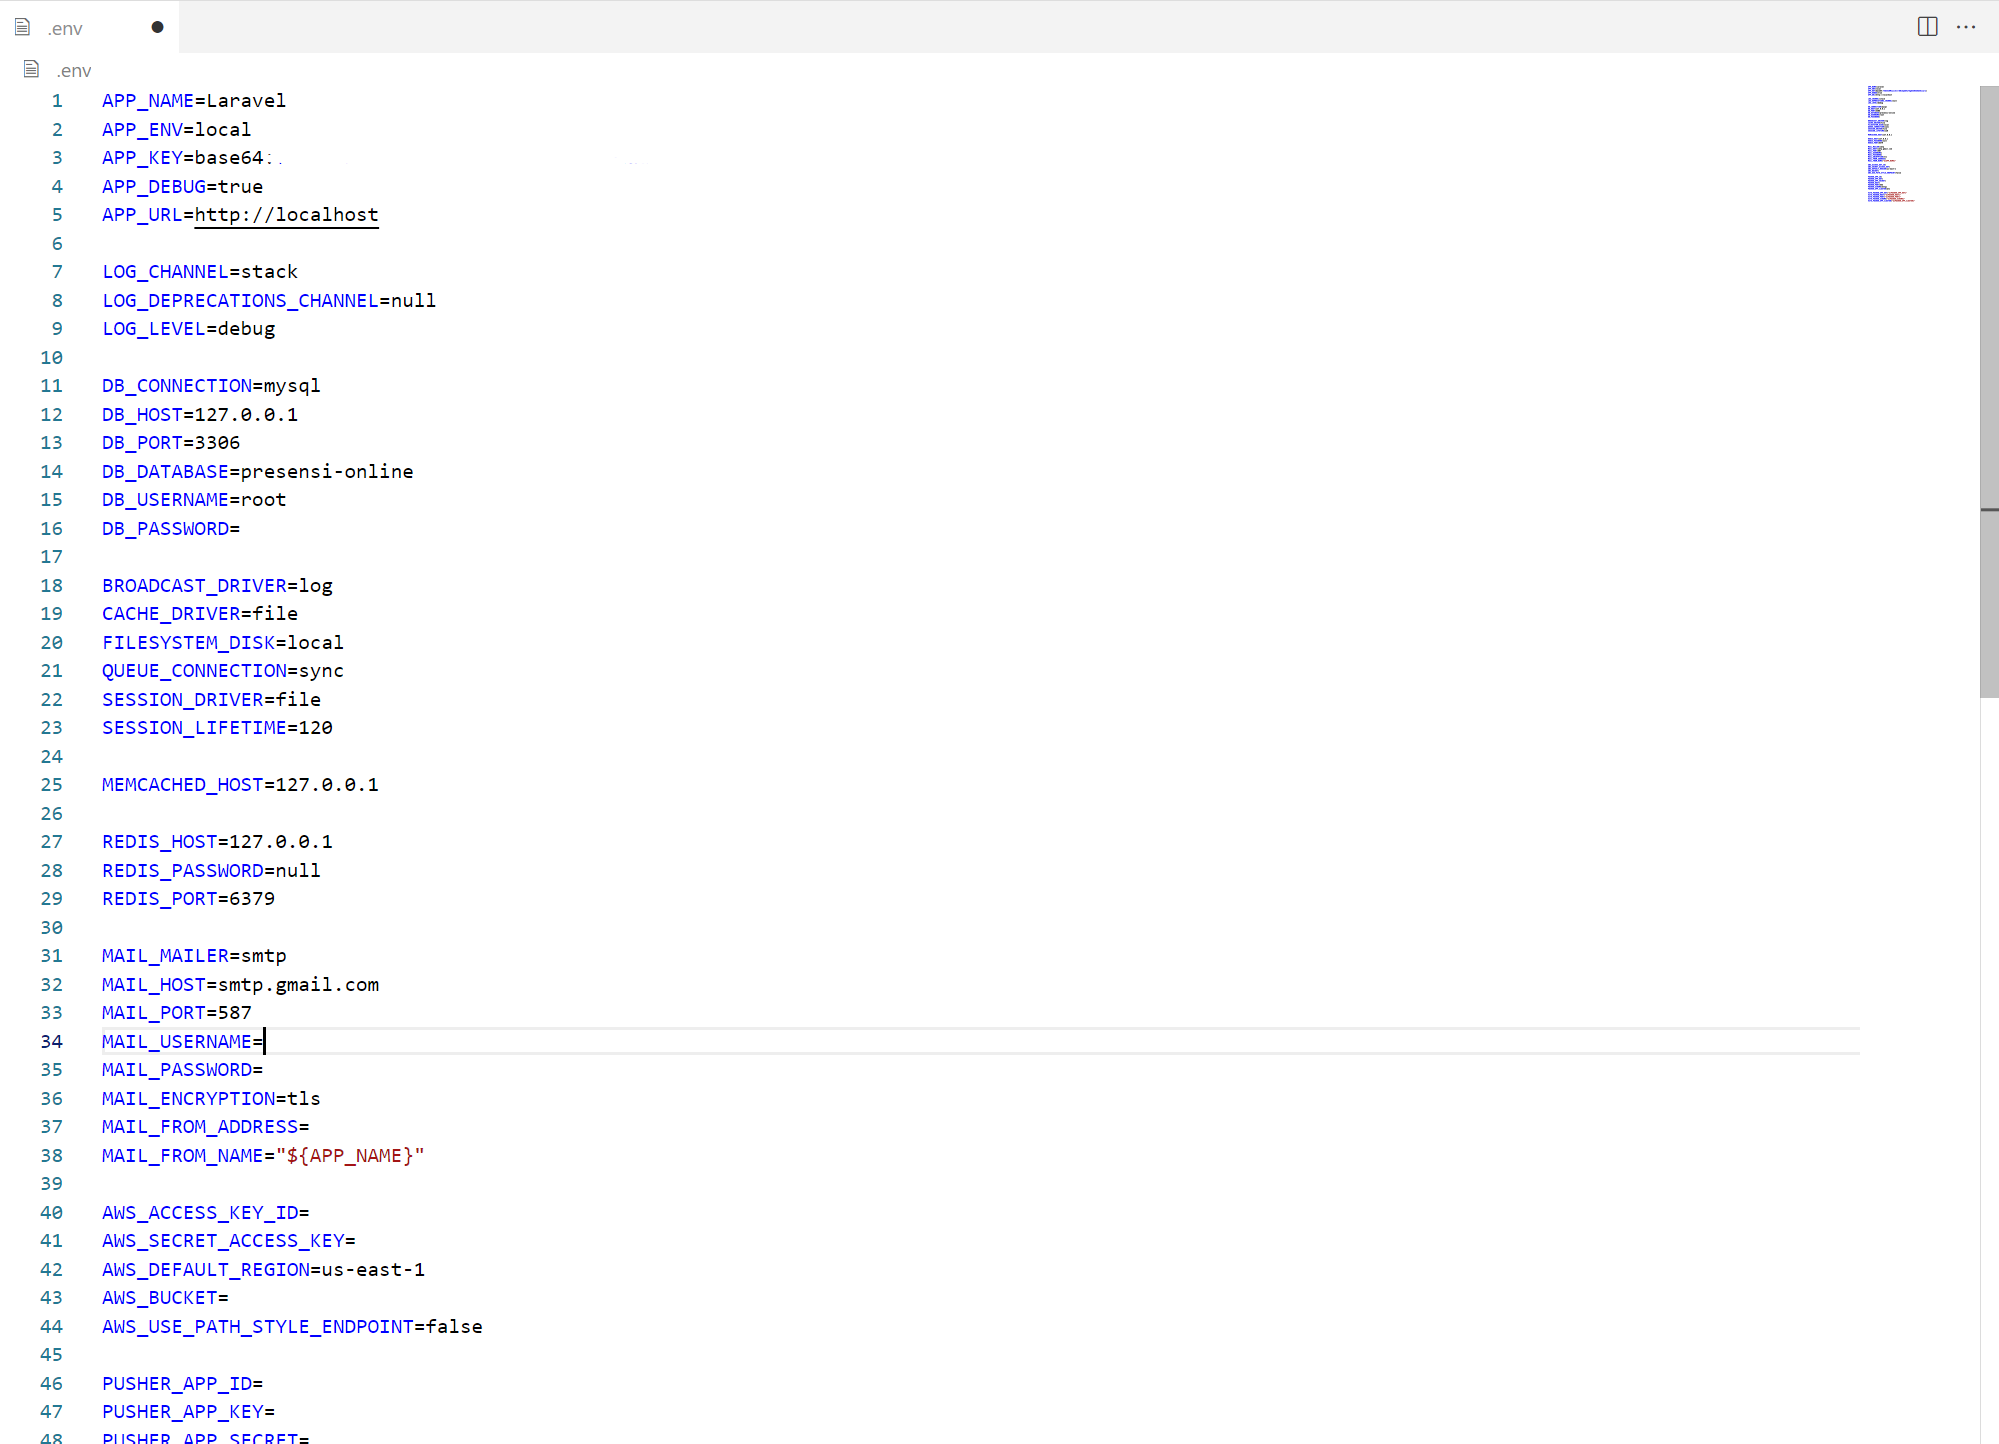
\includegraphics[width=18cm]{Gambar/bab3/file-env.png}
    	\caption{Kode \textit{File} .env}
    	\label{fig:tampilan-file-env}
    \end{figure}
    \FloatBarrier
    %
    %
    \begin{figure}[!htbp]
    	\centering
    	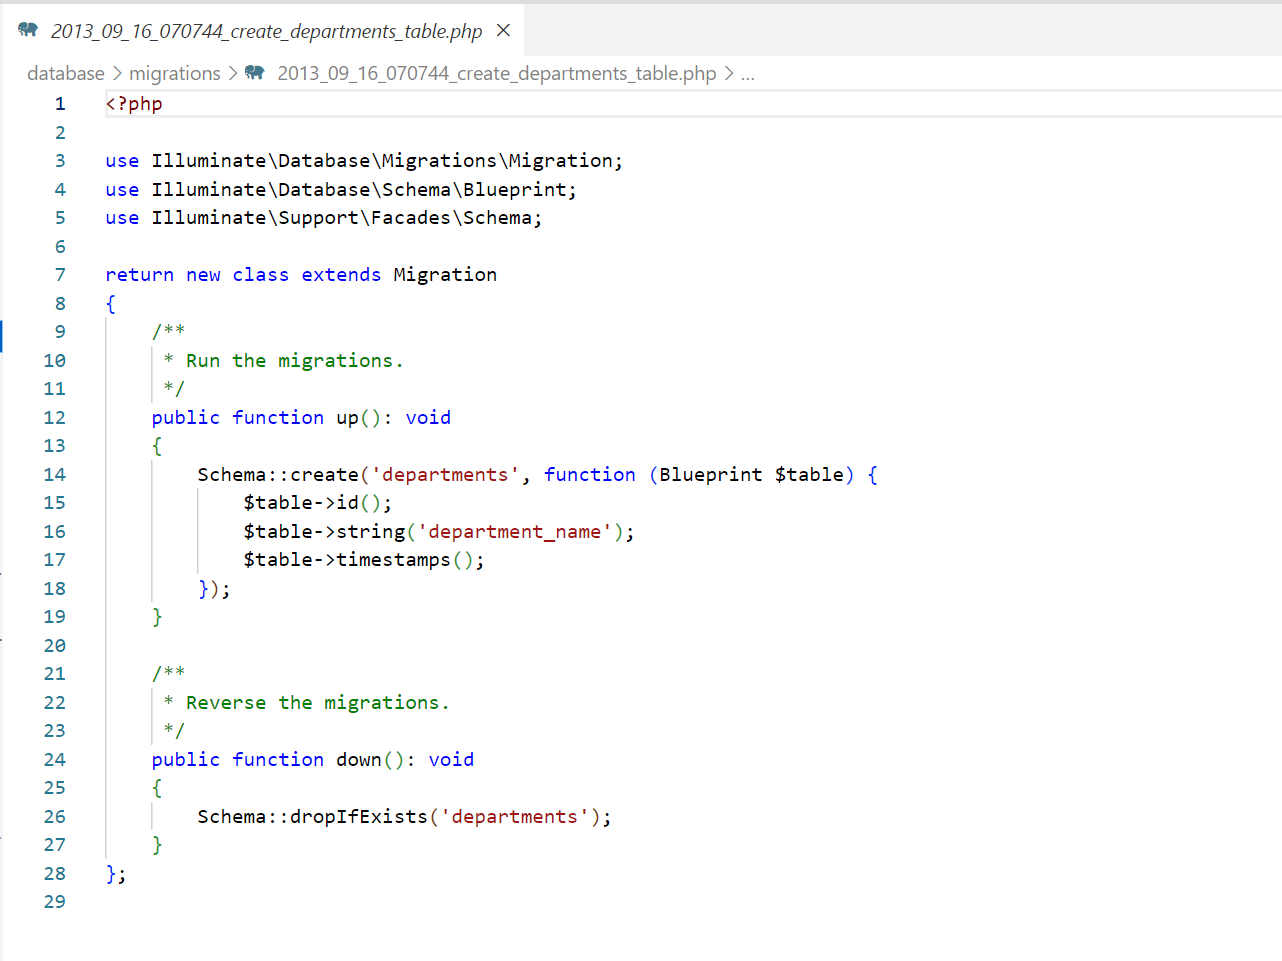
\includegraphics[width=10cm]{Gambar/bab3/migration-department.png}
    	\caption{Kode \textit{Migration} \textit{Department}}
    	\label{fig:tampilan-migration-department}
    \end{figure}
    \FloatBarrier
    %
    %
    \begin{figure}[!htbp]
    	\centering
    	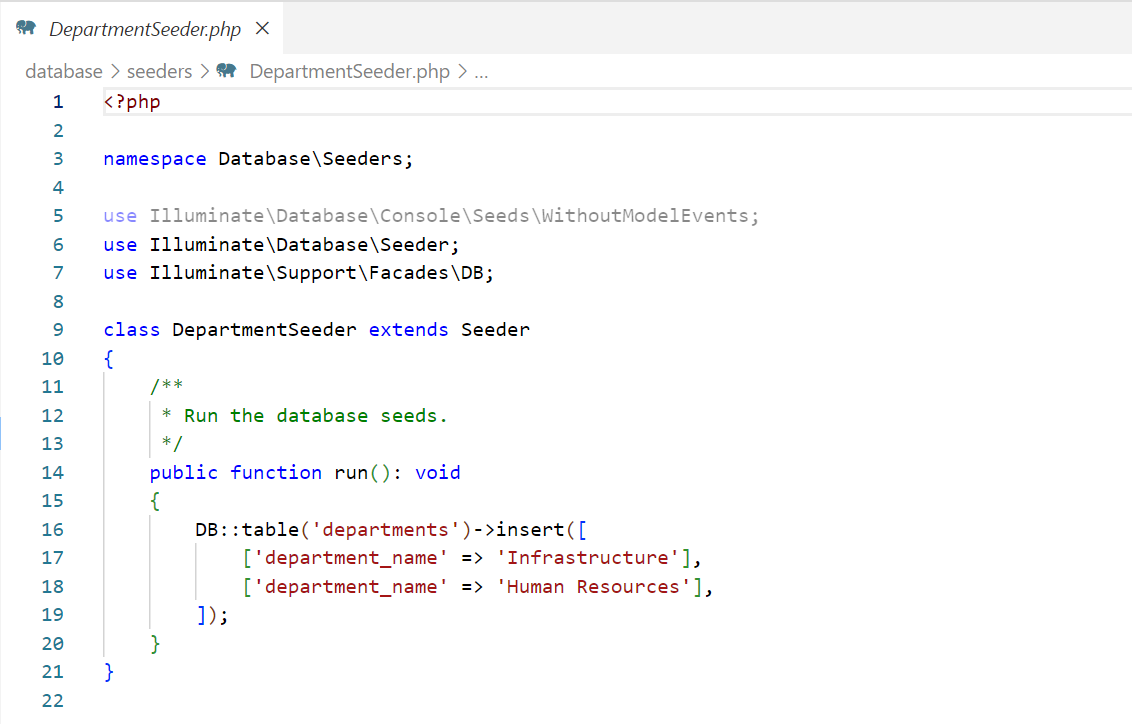
\includegraphics[width=10cm]{Gambar/bab3/seeder-department.png}
    	\caption{Kode \textit{Seeder} \textit{Department}}
    	\label{fig:tampilan-seeder-department}
    \end{figure}
    \FloatBarrier
    %

\subsection{Implementasi Setiap Modul Pada Aplikasi}
Pengembangan aplikasi presensi \textit{online} akan dilakukan per modul seperti modul presensi, \textit{shift}, riwayat presensi, riwayat lembur, dan modul lainnya. Pengembangan aplikasi akan menggunakan \textit{framework} Laravel yang menerapkan konsep MVC (\textit{Model-View-Controller}). \textit{Model} merupakan komponen yang berfungsi mengelola data dan logika bisnis aplikasi. \textit{Model} berinteraksi dengan \textit{database} untuk menyimpan, mengambil, dan memproses data. Dalam Laravel, terdapat \textit{Eloquent} ORM, yang memungkinkan manipulasi data tanpa menulis SQL secara langsung. \textit{View} merupakan bagian yang bertanggung jawab untuk menampilkan data kepada pengguna dalam bentuk antarmuka pengguna (UI) menggunakan Laravel \textit{Templating Engine}. \textit{Styling} dari setiap modul akan menggunakan \textit{framework} Tailwind CSS dan \textit{library Flowbite}, selain itu, tampilan \textit{pop up} pesan akan menggunakan \textit{library Sweet Alert}. \textit{Controller} berperan sebagai penghubung antara \textit{model} dan \textit{view}. \textit{Controller} menerima \textit{input} dari pengguna (biasanya melalui \textit{request} HTTP), memprosesnya dengan bantuan \textit{model}, dan mengembalikan data ke \textit{view} untuk ditampilkan. Selain itu, terdapat juga \textit{routes} yang akan merespons permintaan HTTP dan menjadi penghubung permintaan tersebut dengan \textit{controller}.

Implementasi setiap modul akan dimulai dengan membuat \textit{controller} yang merupakan \textit{backend} pada aplikasi. Salah satu contoh pembuatan \textit{controller} untuk modul \textit{department} dilakukan dengan menjalankan \textit{command line} "php artisan make:controller DepartmentController". \textbf{~\ref{fig:tampilan-controller-department}} menunjukkan isi \textit{file controller} yang akan mengembalikan ke \textit{view department}. Selanjutnya, daftarkan masing-masing \textit{function} dalam \textit{controller} ke \textit{routes} agar dapat diakses melalui permintaan HTTP. \textbf{~\ref{fig:tampilan-routes-department}} menampilkan kode \textit{routes} agar \textit{controller} pada \textit{function index} dapat diakses melalui permintaan HTTP. Selanjutnya membuat tampilan UI atau \textit{view} menggunakan \textit{blade templating engine} dengan cara membuat \textit{file} baru bernama department.blade.php pada \textit{folder view} kemudian didalamnya berisi kode HTML yang nantinya akan ditampilkan jika pengguna mengakses \textit{route} yang telah ditentukan. \textbf{~\ref{fig:kode-view-department}} menunjukkan kode HTML pada \textit{file department.blade.php} yang dibuat menggunakan \textit{blade templating engine}. \textbf{~\ref{fig:tampilan-view-department}} merupakan tampilan halaman \textit{Department} yang diakses melalui \textit{routes} sebelumnya. 
%
    \begin{figure}[!htbp]
    	\centering
    	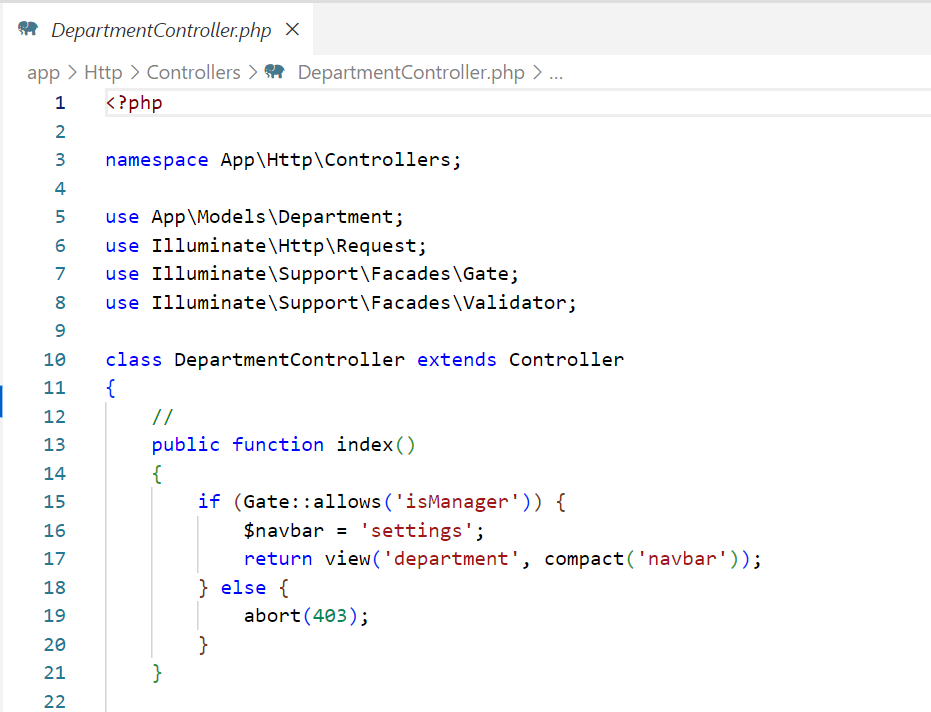
\includegraphics[width=10cm]{Gambar/bab3/controller-department.png}
    	\caption{Kode \textit{Controller} \textit{Department}}
    	\label{fig:tampilan-controller-department}
    \end{figure}
    \FloatBarrier
%
%
    \begin{figure}[!htbp]
    	\centering
    	
\includegraphics[width=10cm]{Gambar/bab3/routes-department.png}
    	\caption{Kode \textit{Routes} \textit{Department}}
    	\label{fig:tampilan-routes-department}
    \end{figure}
    \FloatBarrier
%
%
    \begin{figure}[!htbp]
    	\centering
    	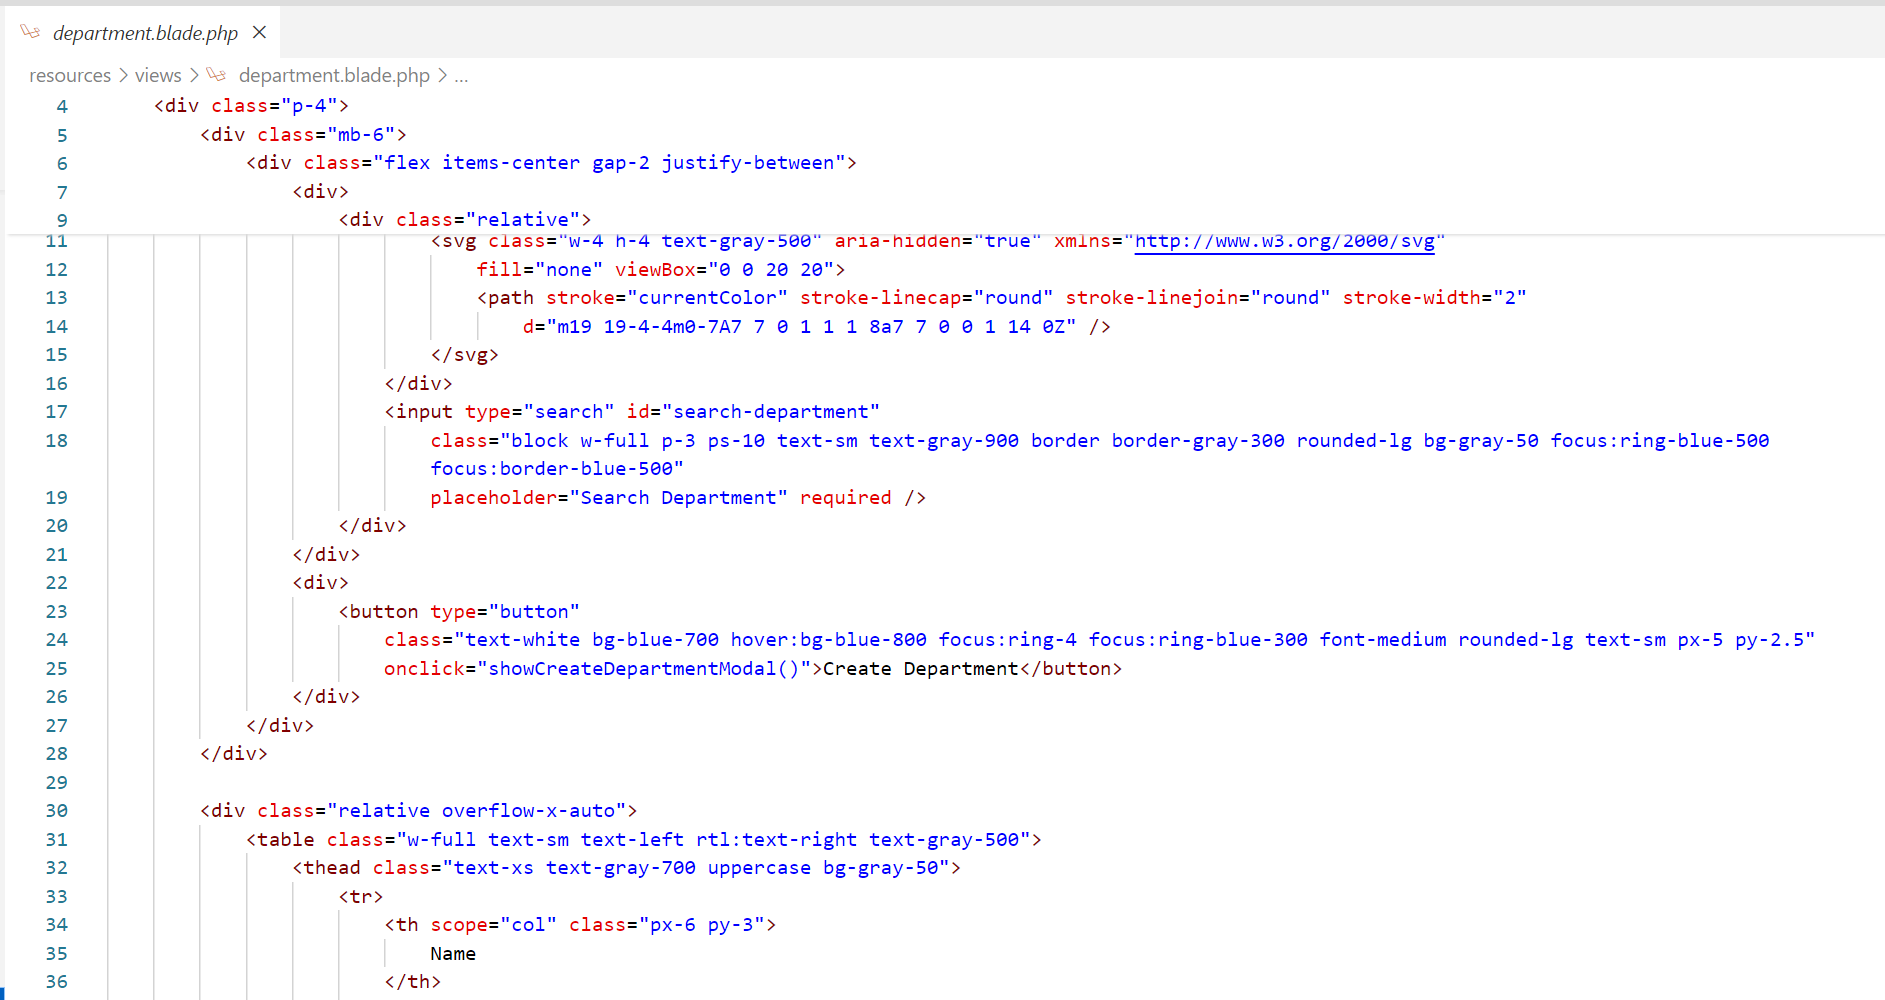
\includegraphics[width=10cm]{Gambar/bab3/view-department.png}
    	\caption{Kode \textit{View} \textit{Department}}
    	\label{fig:kode-view-department}
    \end{figure}
    \FloatBarrier
%
%
    \begin{figure}[!htbp]
    	\centering
    	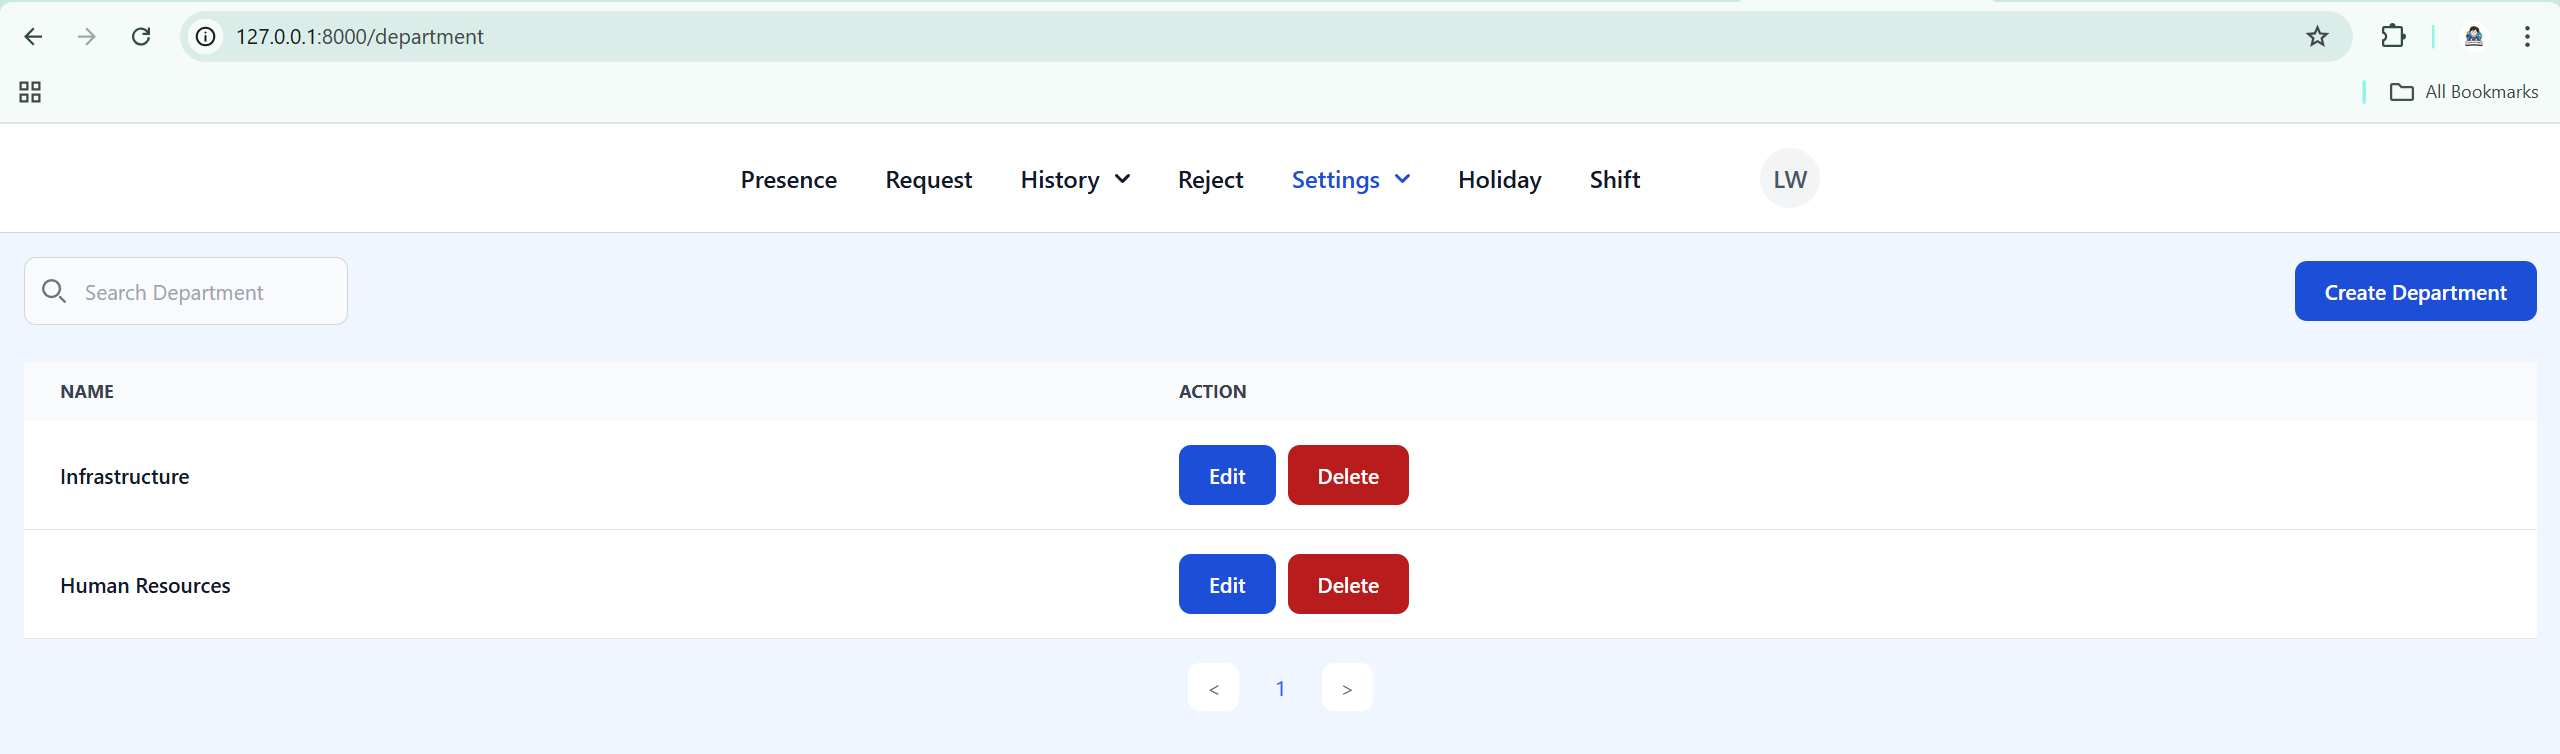
\includegraphics[width=12cm]{Gambar/bab3/tampilan-view-department.png}
    	\caption{Tampilan Halaman \textit{Department}}
    	\label{fig:tampilan-view-department}
    \end{figure}
    \FloatBarrier
%

%
    \begin{figure}[!htbp]
    	\centering
    	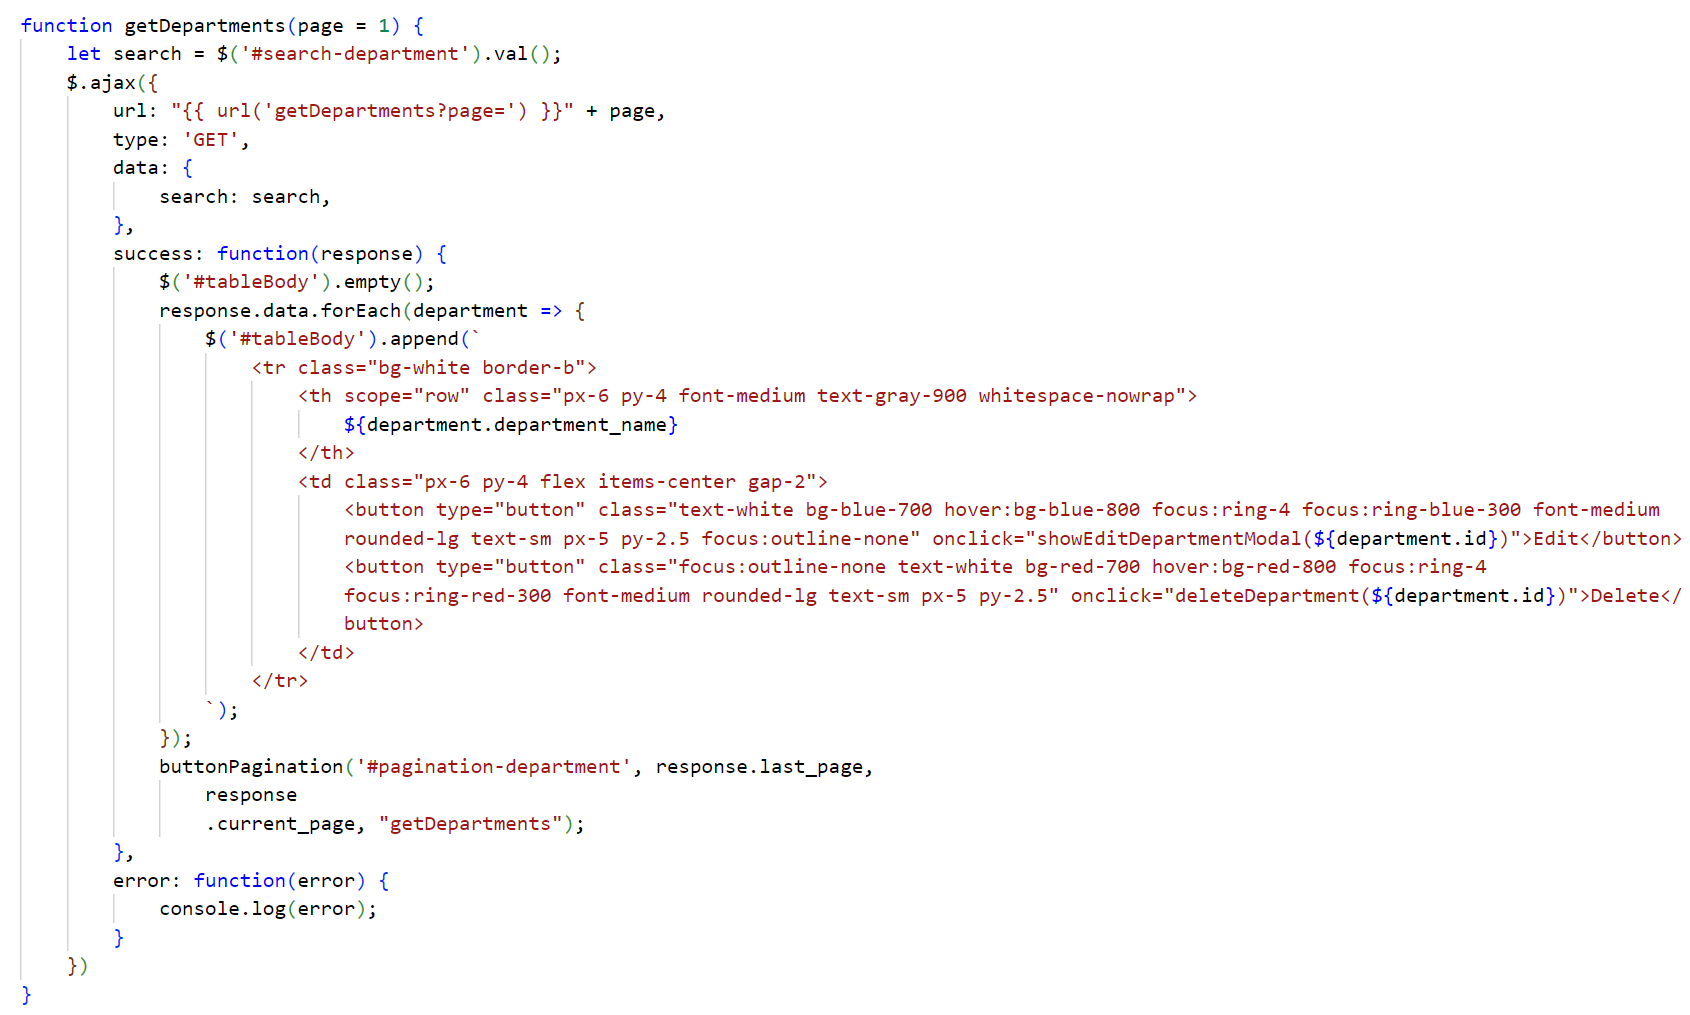
\includegraphics[width=12cm]{Gambar/bab3/ajax-department.png}
    	\caption{Kode AJAX \textit{Fetch} Data \textit{Department}}
    	\label{fig:kode-ajax-department}
    \end{figure}
    \FloatBarrier
%
Dalam setiap modul, pengambilan data akan dilakukan secara terpisah dengan \textit{controller} yang mengembalikan \textit{view}. Pengambilan data akan menggunakan bantuan \textit{library} JavaScript yaitu Jquery AJAX untuk melakukan permintaan HTTP secara \textit{asynchronus} sehingga ketika terjadi penambahan, pengubahan, dan penghapusan data maka halaman tidak ada dimuat kembali melainkan data akan otomatis ter-\textit{update} pada sisi server. \textbf{~\ref{fig:kode-ajax-department}} menampilkan \textit{function} untuk mengambil data \textit{department} secara \textit{asynchronus} menggunakan JQuery AJAX.

\subsection{Implementasi \textit{Geolocation}}
Aplikasi presensi \textit{online} akan mengimplementasi teknologi \textit{Geolocation} untuk mendapatkan titik koordinat lokasi pengguna. Dalam HTML terdapat \textit{Geolocation} API yang dapat digunakan melalui JavaScript tanpa harus meng-\textit{install plugin} tambahan. Dokumenasi penggunaan \textit{Geolocation} API dapat dilihat melalui tautan \url{https://www.w3schools.com/html/html5_geolocation.asp}. \textit{Geolocation} API telah mendukung sebagian banyak \textit{browser modern} seperti \textit{Google Chrome, Safari,} dan lain-lain. \textbf{\ref{fig:kode-geolocation-api}} menunjukkan contoh penggunaan \textit{Geolocation} API pada aplikasi presensi \textit{online} untuk mendapatkan titik koordinat lokasi pengguna.
 \begin{figure}[!htbp]
    	\centering
    	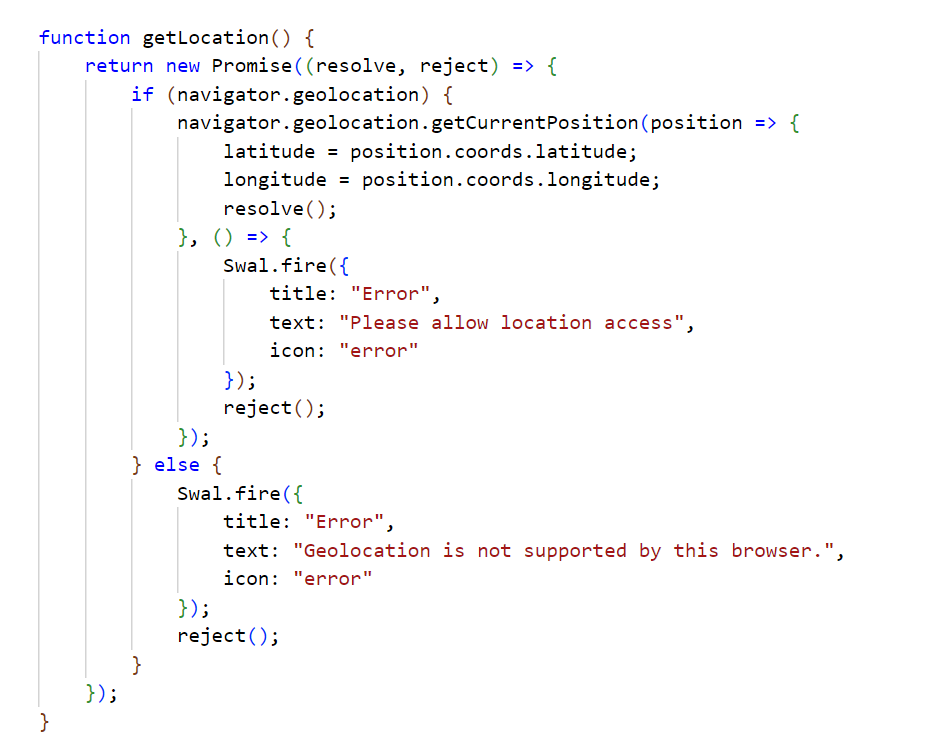
\includegraphics[width=10cm]{Gambar/bab3/kode-geolocation.png}
    	\caption{Kode \textit{Geolocation} API}
    	\label{fig:kode-geolocation-api}
    \end{figure}
    \FloatBarrier

\subsection{Implementasi Peta Interaktif}
Pada aplikasi presensi \textit{online} terdapat gambar peta yang ditampilkan kepada \textit{Staff Infrastructure} saat melakukan presensi. Fungsi peta ini agar \textit{Staff Infrastructure} dapat mengetahui apakah lokasi sudah sesuai dengan posisinya. \textit{library }Leaflet JS akan digunakan pada aplikasi presensi \textit{online} untuk menampilkan gambar peta lokasi \textit{staff}. Dokumentasi \textit{library} Leaflet JS dapat dilihat melalui tautan \url{https://leafletjs.com/reference.html}. Penggunaan \textit{library} Leaflet JS hanya perlu membutuhkan parameter titik koordinat lokasi \textit{Staff Infrastructure} berupa \textit{longitude} dan \textit{latitude} yang telah didapatkan melalui teknologi \textit{Geolocation} API sebelumnya. \textbf{\ref{fig:hasil-leaflet-js}} menunjukkan gambar titik lokasi pengguna yang ditampilkan dalam bentuk peta menggunakan \textit{library} Leaflet JS.
\begin{figure}[!htbp]
    	\centering
    	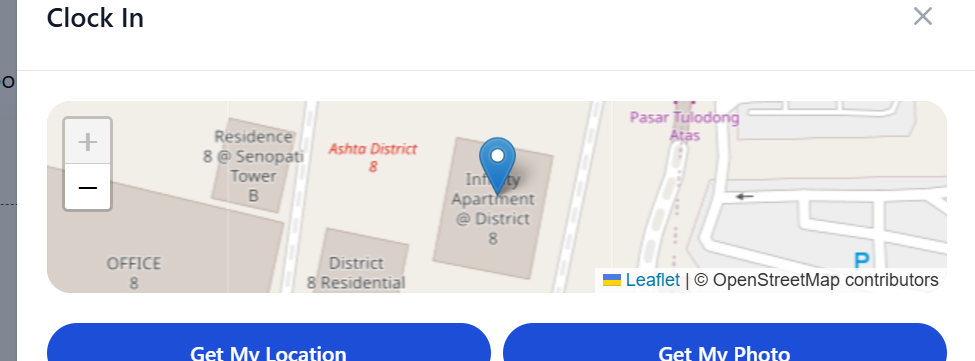
\includegraphics[width=15cm]{Gambar/bab3/hasil-leaflet-js.png}
    	\caption{Hasil Gambar Peta Lokasi Menggunakan Leaflet JS}
    	\label{fig:hasil-leaflet-js}
    \end{figure}
    \FloatBarrier
    
\subsection{Implementasi Perhitungan Jarak}
Aplikasi ini akan mengimplementasikan algoritma Haversine. Algoritma Haversine akan digunakan untuk menghitung jarak antara lokasi pengguna saat presensi dengan lokasi kantor. Lokasi pengguna akan didapatkan melalui teknologi \textit{Geolocation} API yang telah diimplementasikan sebelumnya. Hasil dari perhitungan akan memberikan keterangan pada presensi yaitu "\textit{In Office}" jika pengguna melakukan presensi di sekitar radius kantor dan "\textit{Out Office}" jika pengguna melakukan presensi di luar radius kantor. Jarak toleransi akan diberikan sebesar 120 meter. \textbf{~\ref{fig:kode-function-haversine}} menunjukkan kode \textit{function} Haversine yang akan digunakan untuk menghitung kedua jarak. \textbf{~\ref{fig:tampilan-keterangan-presensi}} menampilkan tampilan keterangan presensi yaitu "\textit{In Office}" dan "\textit{Out Office}" yang didapat melalui perhitungan algoritma Haversine pada halaman riwayat presensi.
%
    \begin{figure}[!htbp]
    	\centering
    	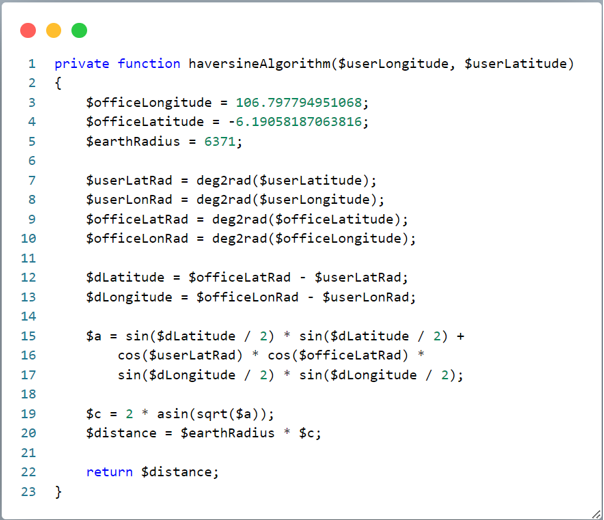
\includegraphics[width=10cm]{Gambar/bab3/function-haversine.png}
    	\caption{Kode \textit{Function} Haversine}
    	\label{fig:kode-function-haversine}
    \end{figure}
    \FloatBarrier
%
%
    \begin{figure}[!htbp]
    	\centering
    	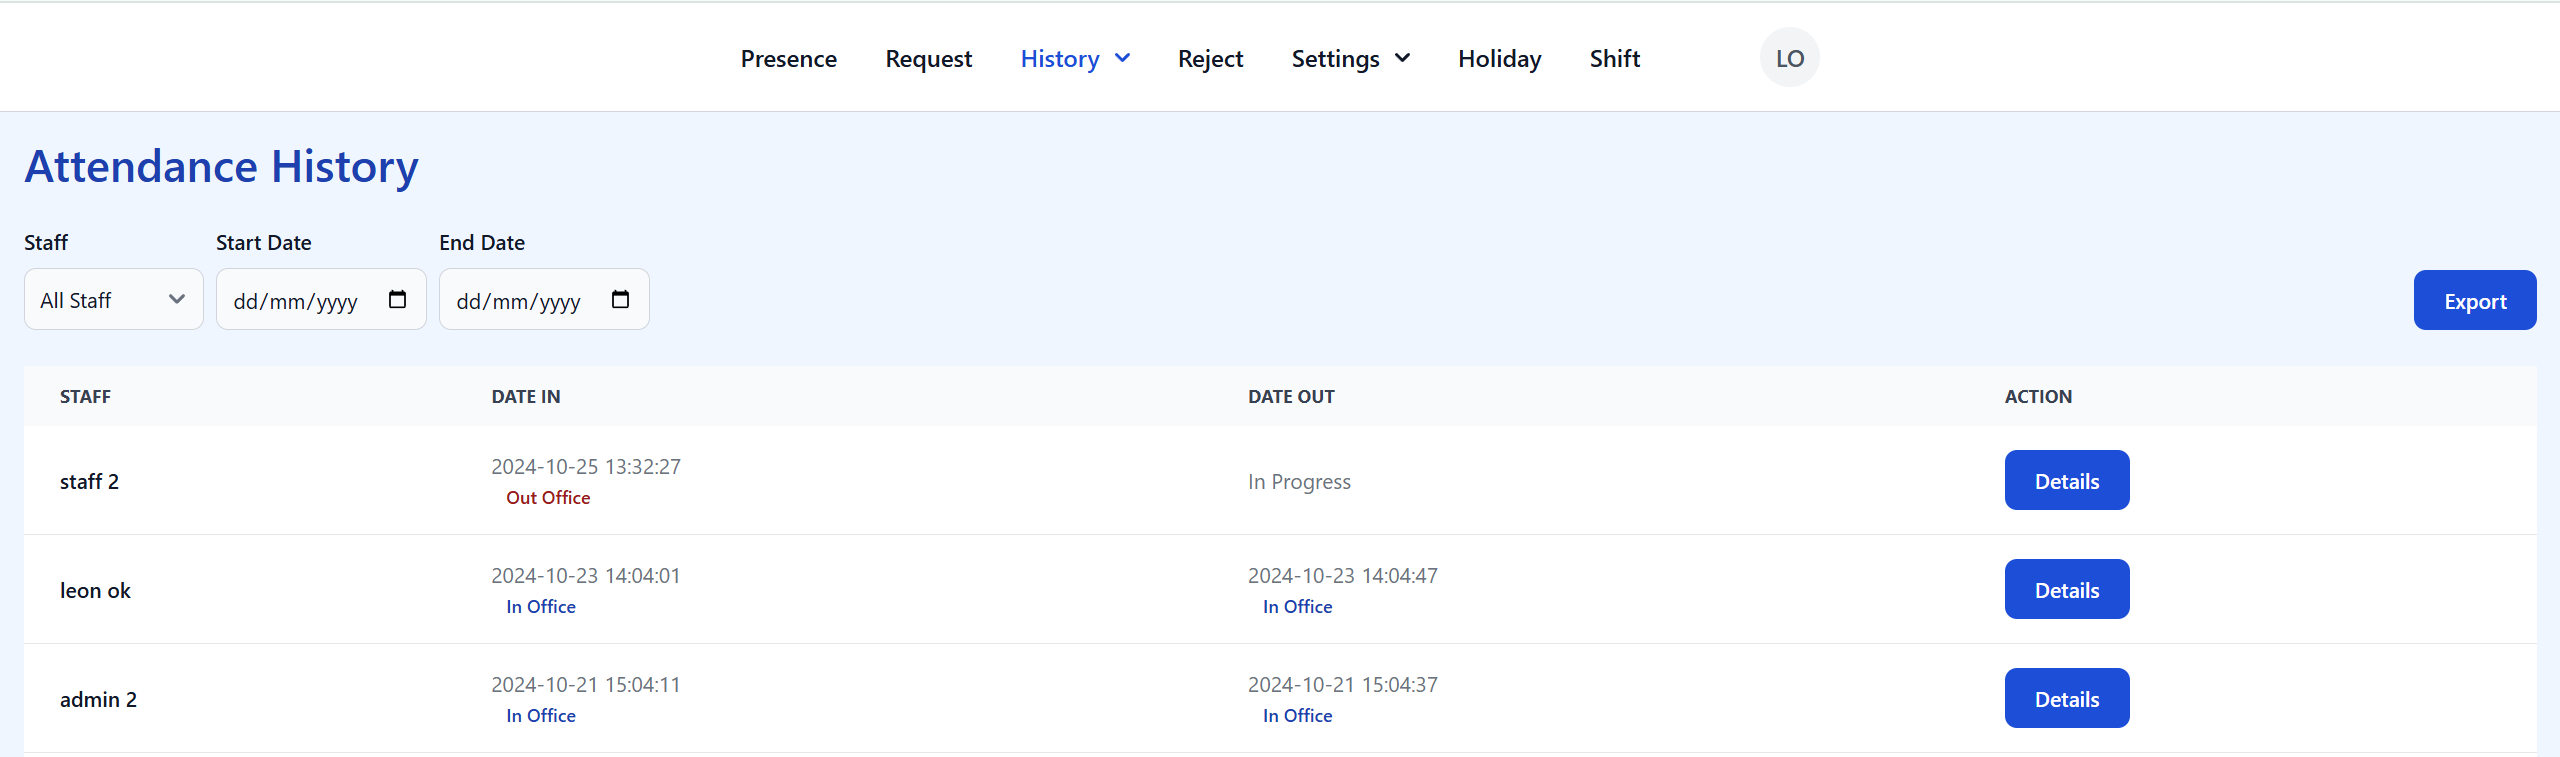
\includegraphics[width=15cm]{Gambar/bab3/tampilan-keterangan-presensi.png}
    	\caption{Tampilan Keterangan Presensi}
    	\label{fig:tampilan-keterangan-presensi}
    \end{figure}
    \FloatBarrier
%



\subsection{Implementasi Validasi Wajah}
Pada aplikasi presensi \textit{online} akan terdapat fitur untuk pengambilan wajah saat \textit{staff} melakukan presensi. Aplikasi presensi akan menggunakan teknologi WebRTC sebagai kamera menggunakan JavaScript tanpa perlu meng-\textit{install} \textit{plugin} tambahan. Penggunaan teknologi WebRTC ini agar pengambilan wajah dilakukan secara langsung saat presensi sehingga tidak terjadi kecurangan seperti meng-\textit{upload file} foto pada galeri pengguna. \textbf{\ref{fig:kode-webrtc}} menunjukkan kode \textit{function} untuk membuka mengakses kamera depan menggunakan teknologi WebRTC.
\begin{figure}[!htbp]
    	\centering
    	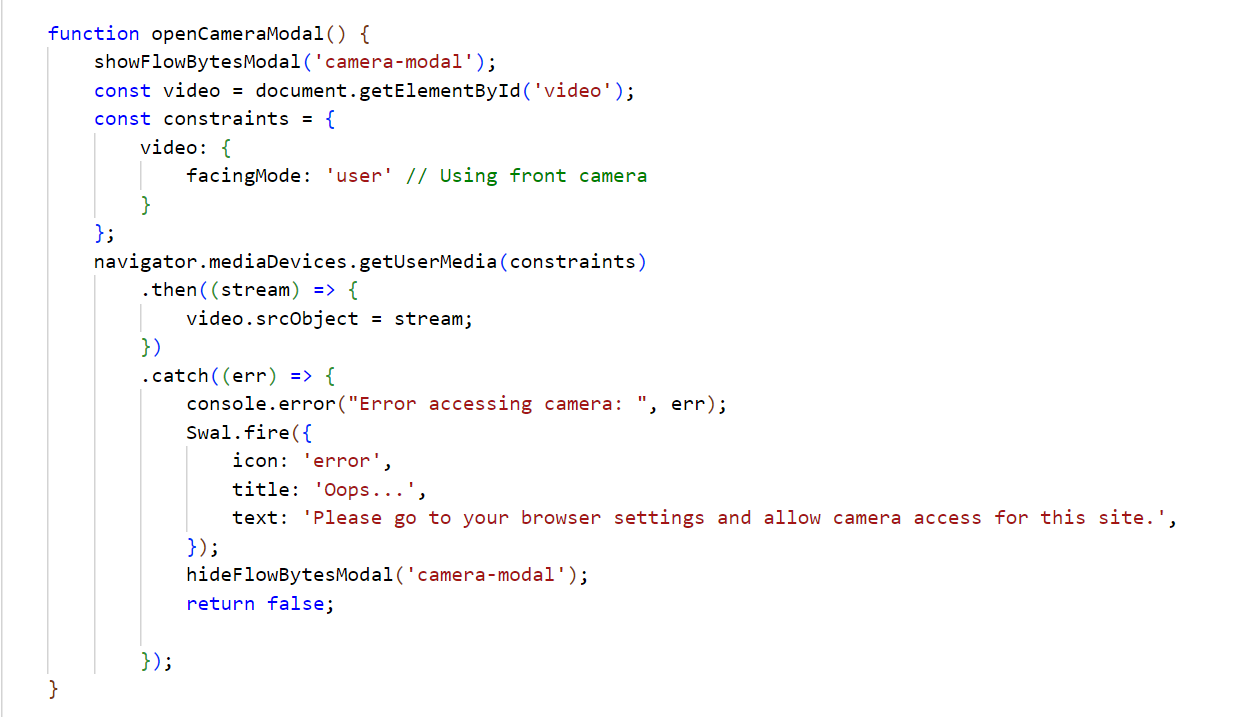
\includegraphics[width=15cm]{Gambar/bab3/kode-webrtc-kamera.png}
    	\caption{Kode WebRTC Pada Kamera}
    	\label{fig:kode-webrtc}
    \end{figure}
    \FloatBarrier
Selain itu, aplikasi presensi \textit{online} akan menerapkan TensorFlow. TensorFlow merupakan \textit{framework open-source} yang dikembangkan oleh \textit{Google} untuk komputasi numerik dan \textit{machine learning}, terutama \textit{deep learning}. Pada aplikasi presensi \textit{online} akan menerapkan \textit{model BlazeFace} yang merupakan \textit{model deep learning} yang dikembangkan oleh \textit{Google} untuk mendeteksi wajah dengan cepat dan efisien, terutama pada perangkat seluler. Penggunaan \textit{model} ini cukup mudah yaitu dengan menyisipkan kode script CDN pada aplikasi yang dapat dilihat pada \textbf{~\ref{fig:kode-script-cdn-tensorflow}}.
%
    \begin{figure}[!htbp]
    	\centering
    	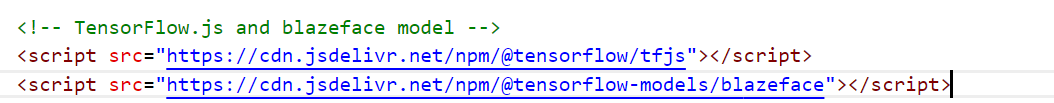
\includegraphics[width=15cm]{Gambar/bab3/cdn-tensorflow.png}
    	\caption{Kode Script CDN TensorFlow dan \textit{Model BlazeFace}}
    	\label{fig:kode-script-cdn-tensorflow}
    \end{figure}
    \FloatBarrier
%
Setelah itu, memasukkan kode logika yang digunakan untuk mengecek wajah pada saat pengambilan foto melalui kamera saat presensi. \textbf{~\ref{fig:kode-function-pengambilan-foto}} menunjukkan kode pengambilan foto saat presensi, dalam \textit{function} tersebut akan dilakukan pengecekkan wajah pada kamera menggunakan TensorFlow. Foto yang diambil akan divalidasi seperti harus terdapat wajah pada kamera, tidak boleh terlalu dekat dengan kamera, dan posisi wajah harus berada ditengah kamera saat pengambilan foto.
%
    \begin{figure}[!htbp]
    	\centering
    	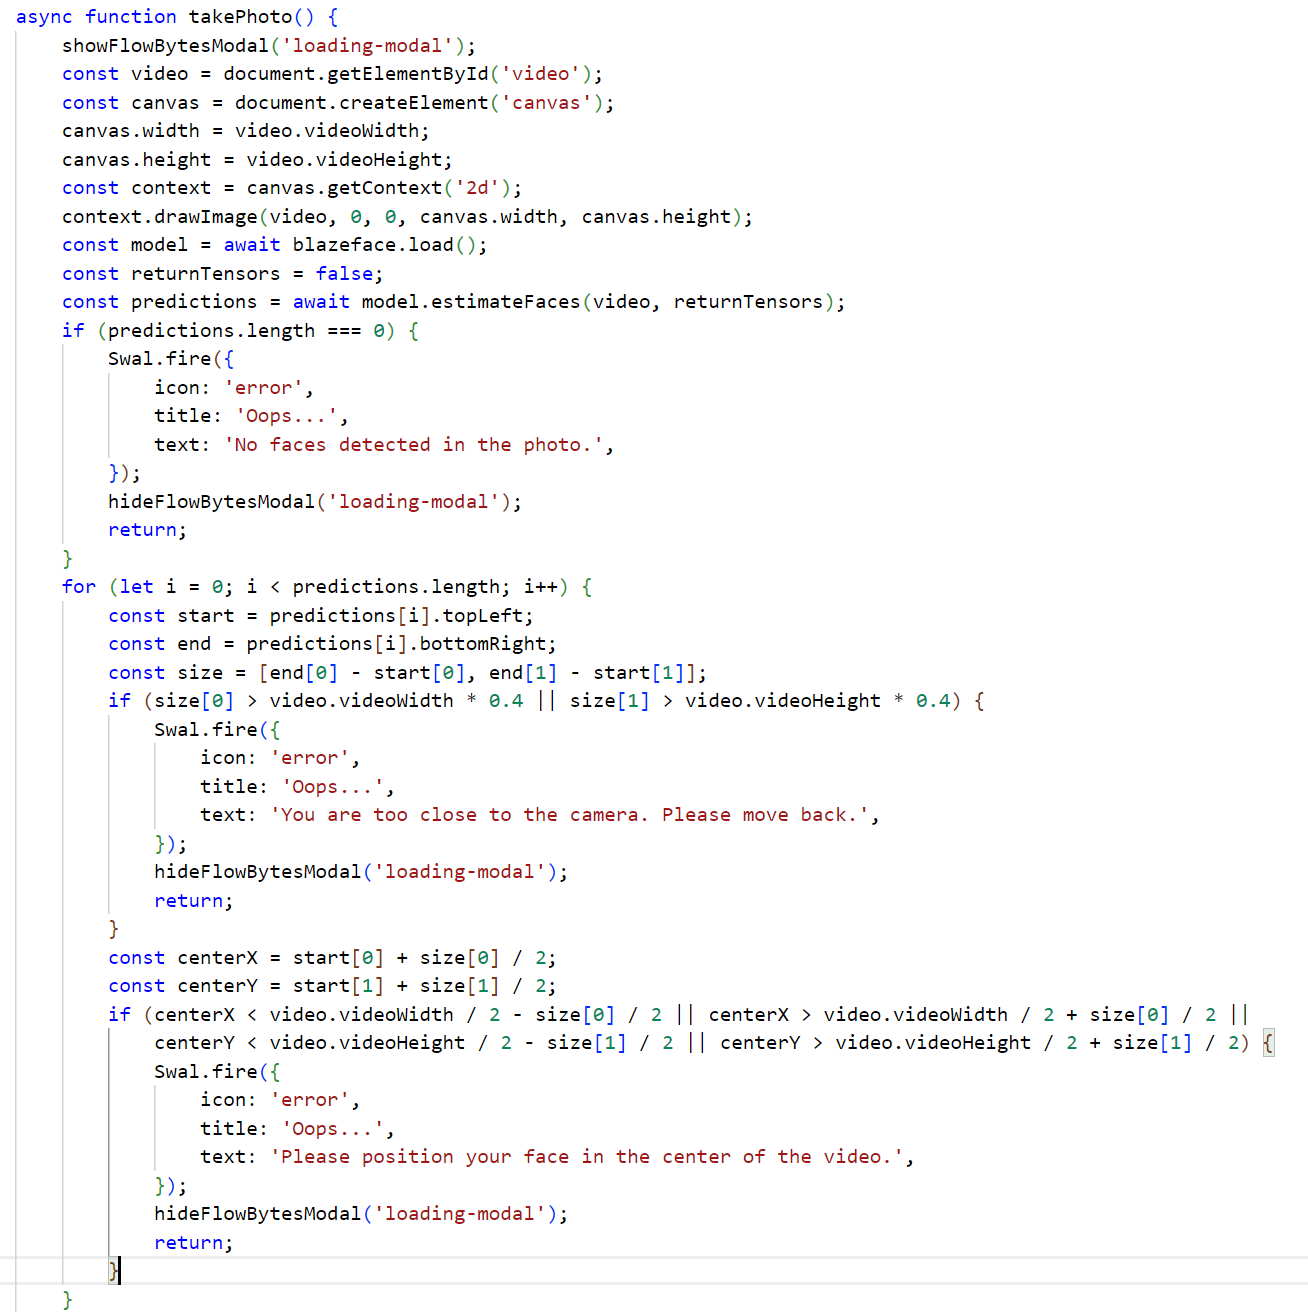
\includegraphics[width=9cm]{Gambar/bab3/function-cek-wajah.png}
    	\caption{Kode \textit{Function} Pengambilan Foto}
    	\label{fig:kode-function-pengambilan-foto}
    \end{figure}
    \FloatBarrier
%
Tampilan modal kamera yang sudah diintegrasi dengan TensorFlow dapat dilihat pada \textbf{~\ref{fig:tampilan-kamera-integrasi-tensorflow}}. Pada tampilan kamera tersebut posisi wajah harus berada dilingkaran putih yang sudah ditentukan. Jika tidak terdapat wajah pada saat pengambilan foto atau posisi wajah tidak berada di tengah kamera, serta posisi wajah terlalu dekat dengan kamera maka akan menampilkan pesan \textit{error} yang dapat dilihat pada \textbf{~\ref{fig:tampilan-error-validasi-pengambilan-foto}}. Maka pengguna harus melakukan pengambilan foto wajah ulang, hingga sistem berhasil mendeteksi wajah pada kamera.
%
    \begin{figure}[!htbp]
    	\centering
    	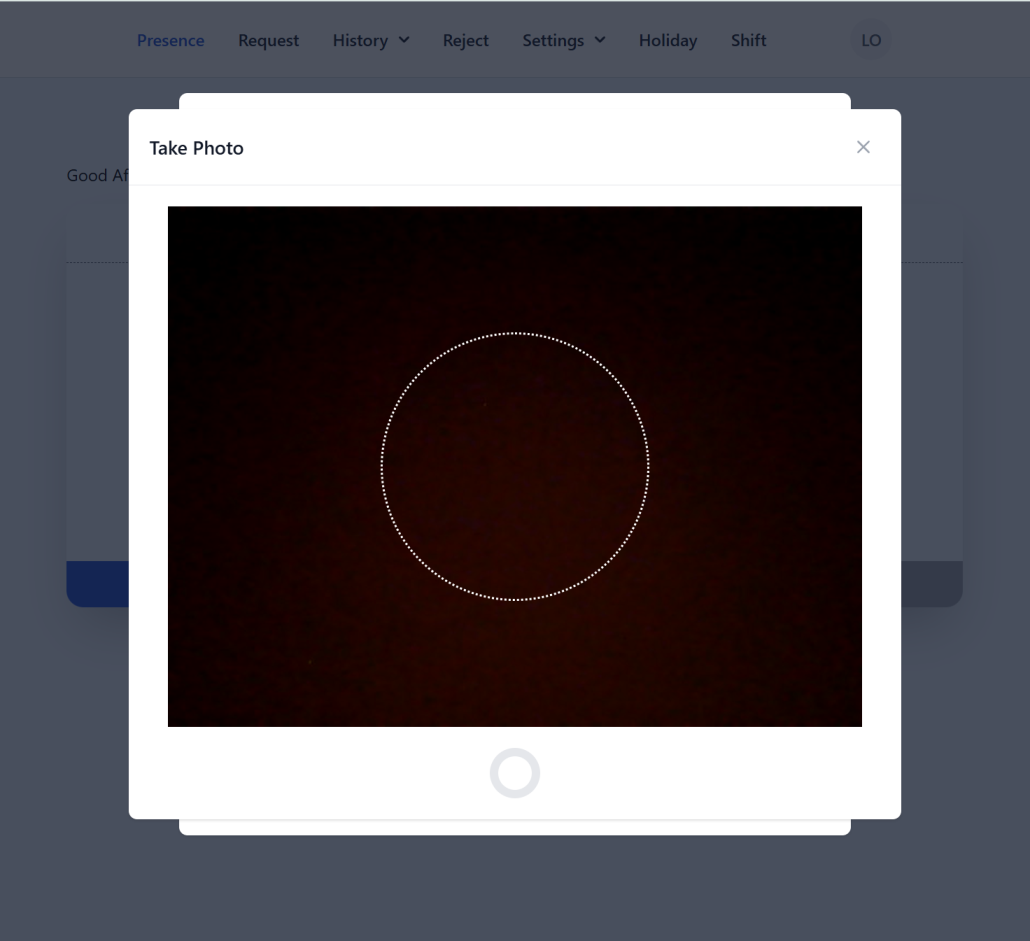
\includegraphics[width=7cm]{Gambar/bab3/modal-kamera-tensorflow.png}
    	\caption{Tampilan Modal Kamera Integrasi TensorFlow}
    	\label{fig:tampilan-kamera-integrasi-tensorflow}
    \end{figure}
    \FloatBarrier
%
%
    \begin{figure}[!htbp]
    	\centering
    	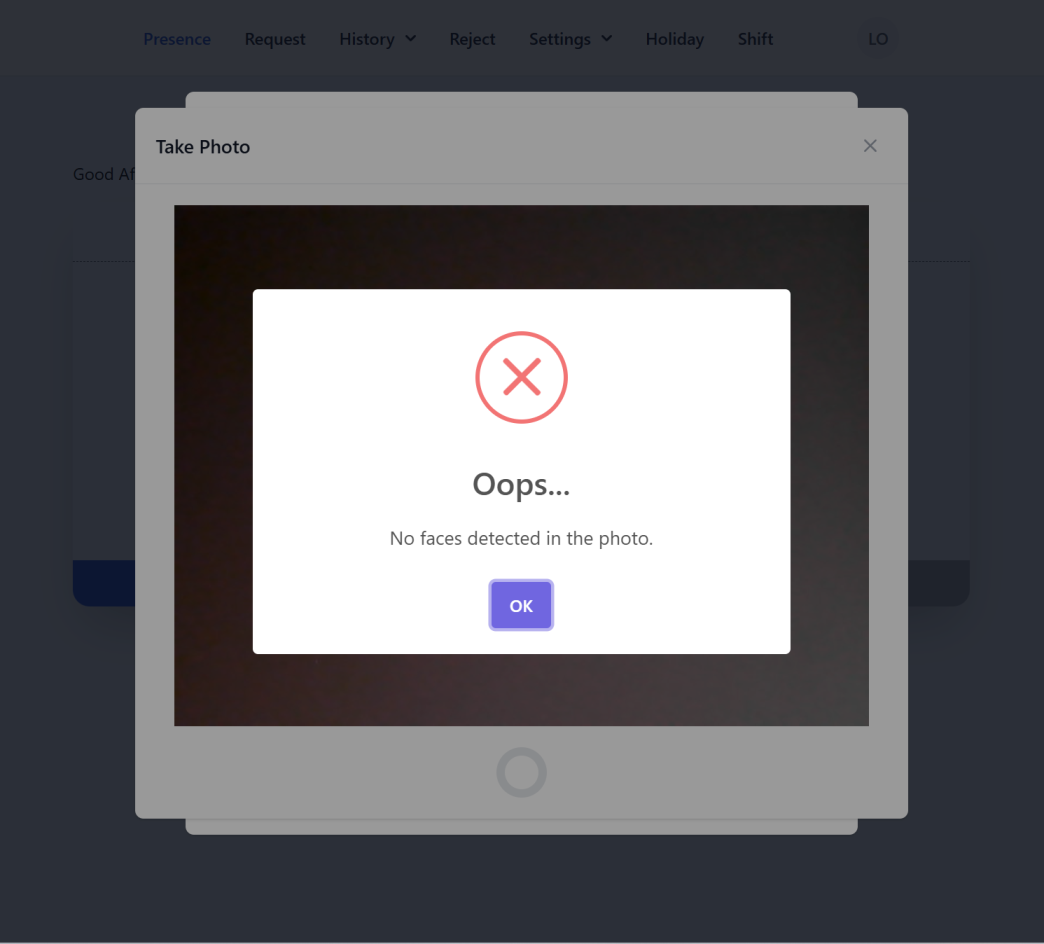
\includegraphics[width=7cm]{Gambar/bab3/no-faces-kamera-tensorflow.png}
    	\caption{Tampilan Validasi \textit{Error} Pengambilan Foto}
    	\label{fig:tampilan-error-validasi-pengambilan-foto}
    \end{figure}
    \FloatBarrier
%
\subsection{Implementasi Perhitungan Lembur Otomatis}
Pada aplikasi presensi \textit{online} akan dilengkapi perhitungan lembur otomatis ketika \textit{Staff Infrastructure} melakukan presensi masuk dan keluar diluar jam kerja \textit{shift} atau pada hari libur perusahaan. Setiap \textit{Staff Infrastructure} akan diatur jenis \textit{shift} yang akan digunakan berdasarkan kurun waktu tertentu. \textbf{\ref{fig:tampilan-pengaturan-jadwal-shift}} menunjukkan halaman modul penjadwalan \textit{shift} yang berisi data nama \textit{staff} "leon ok" akan menggunakan jenis \textit{shift} "password clock" dari tanggal 1 November 2024 hingga 30 November 2024.
 \begin{figure}[!htbp]
    	\centering
    	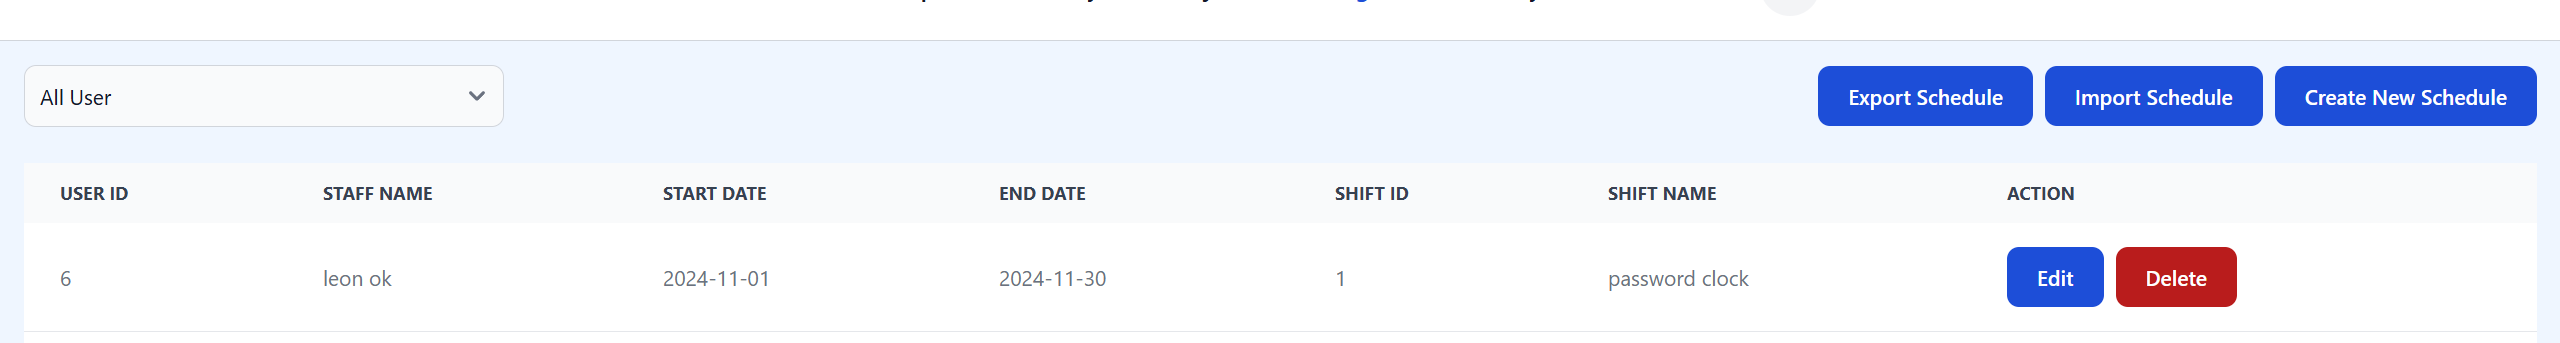
\includegraphics[width=7cm]{Gambar/bab3/implementasi-jadwal-shift.png}
    	\caption{Tampilan Pengaturan Jadwal \textit{Shift}}
    	\label{fig:tampilan-pengaturan-jadwal-shift}
    \end{figure}
    \FloatBarrier
Selanjutnya, masing-masing \textit{Staff Infrastructure} akan diatur jadwal libur yang bisa saja sama antara \textit{staff} satu dengan lainnya maupun sebaliknya. \textbf{\ref{fig:tampilan-pengaturan-libur-staff-infrastructure}} menunjukkan pengaturan jenis libur yang digunakan oleh pengguna.
\begin{figure}[!htbp]
    	\centering
    	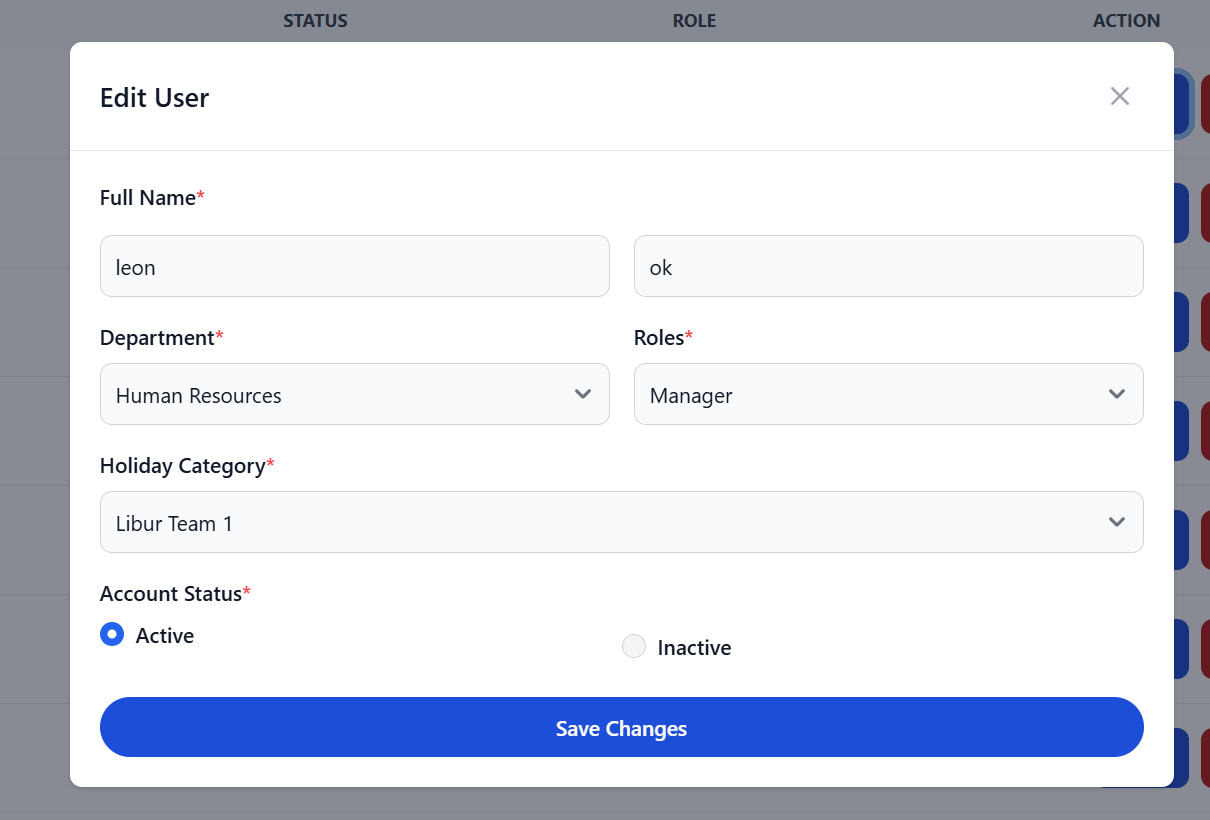
\includegraphics[width=7cm]{Gambar/bab3/implementasi-pengaturan-libur.png}
    	\caption{Tampilan Pengaturan Libur Pada \textit{Staff Infrastructure}}
    	\label{fig:tampilan-pengaturan-libur-staff-infrastructure}
    \end{figure}
    \FloatBarrier

Setelah mengatur penjadwalan \textit{shift} dan libur pada setiap pengguna, maka aplikasi presensi \textit{online} akan otomatis mengecek tanggal dan waktu pengguna setiap melakukan presensi keluar dan membuat data lembur secara otomatis jika presensi dilakukan diluar penjadwalan \textit{shift} yang telah ditentukan ataupun saat hari libur perusahaan. \textbf{\ref{fig:tampilan-lembur-otomatis}} menunjukkan tampilan modal yang memberikan informasi lembur yang dibuat secara otomatis, sistem juga otomatis menghitung total lembur \textit{Staff Infrastructure} dalam satuan menit.
\begin{figure}[!htbp]
    	\centering
    	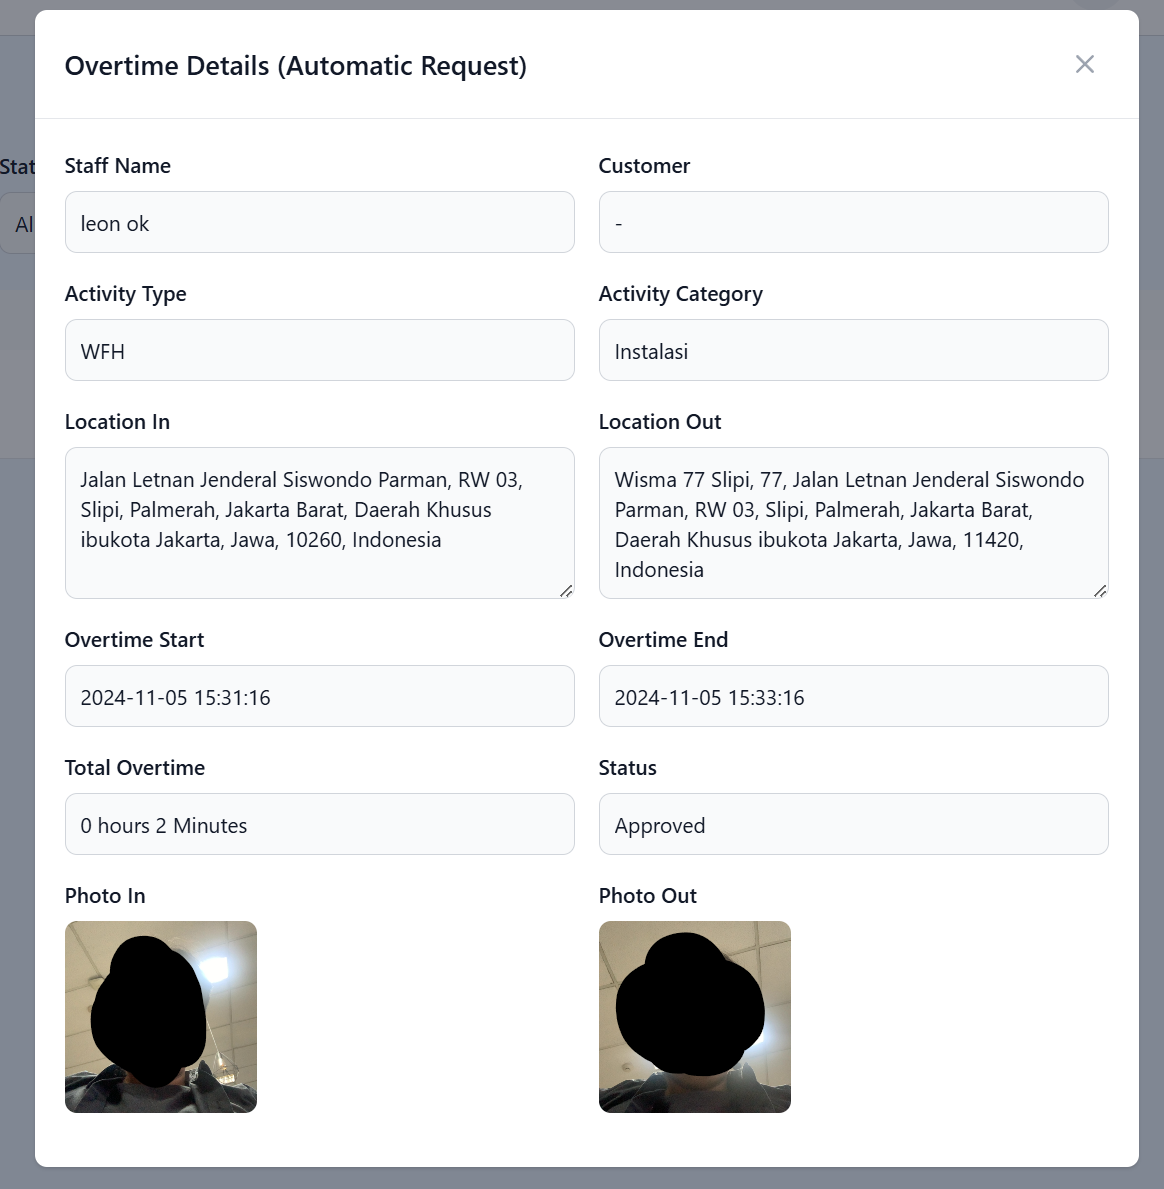
\includegraphics[width=7cm]{Gambar/bab3/implementasi-lembur-otomatis.png}
    	\caption{Tampilan Modal Informasi Lembur Secara Otomatis}
    	\label{fig:tampilan-lembur-otomatis}
    \end{figure}
    \FloatBarrier

\subsection{Implementasi Otorisasi}
Setelah seluruh modul selesai dibuat, maka akan dibuat \textit{middleware} yang berguna untuk membatasi akses modul yang dapat digunakan oleh pengguna. Dalam aplikasi presensi \textit{online} akan terdapat beberapa otorisasi yang digunakan yaitu sebagai berikut:
\begin{enumerate}
    \item \textit{Guest}
    \\ Otorisasi ini berfungsi untuk memberikan akses modul pada pengguna yang belum melakukan autentikasi, seperti modul registrasi dan \textit{login}. 

    \item \textit{Auth}
    \\ Otorisasi ini berfungsi untuk membatasi akses seluruh modul yang mengharuskan pengguna untuk melakukan \textit{authentication} dengan status akun yang telah diverifikasi \textit{email}-nya.
    
    \item \textit{CheckIsActive}
    \\ Otorisasi ini berfungsi untuk mengecek akun pengguna. Jika akun pengguna dengan status \textit{active}, maka dapat mengakses modul sesuai dengan \textit{role} yang diberikan. Jika status \textit{inactive}, maka tidak dapat mengakses seluruh modul dan harus menunggu hingga akun diaktifkan oleh \textit{Manager}.

    \item \textit{CheckSession}
    \\ Otorisasi ini akan mengecek sesi pengguna, jika sebelumnya pengguna sudah melakukan \textit{login} dan kemudian ingin melakukan \textit{login} pada \textit{device} berbeda, maka sesi pada perangkat yang lama akan otomatis ter-\textit{logout}.

    \item \textit{IsManager}
    \\ Otorisasi ini akan membatasi modul yang hanya dapat diakses oleh \textit{role Manager}, seperti \textit{settings department} dan \textit{user}, \textit{shift}, \textit{reject}, dan \textit{holiday}.
\end{enumerate}

\subsection{\textit{Deployment} Aplikasi}
Pada tahap \textit{deployment} aplikasi secara lokal akan menggunakan Artisan CLI yang merupakan salah satu fitur dari Laravel. Cara menjalankan aplikasi dengan server lokal dengan mengetikkan \textit{command line} "php artisan serve". Setelah itu mengatur konfigurasi pada \textit{file} .env yaitu mengubah value APP\_ENV menjadi \textit{local} dan APP\_DEBUG menjadi \textit{true} agar dapat memantau \textit{error} secara langsung. Sedangkan pada \textit{deployment} pada \textit{production} akan menggunakan CPanel. \textit{File project} akan di-\textit{upload} melalui \textit{file manager}. Setelah itu, mengatur \textit{folder public} sebagai \textit{root domain} dan melakukan penyesuaian pada lokasi direktori \textit{folder public} pada \textit{file} autoload.php. Pada \textit{file} .env akan dilakukan konfigurasi berupa APP\_ENV menjadi \textit{production} dan APP\_DEBUG menjadi \textit{false} agar ketika terjadi \textit{error} maka tidak akan memberikan pesan \textit{error} secara detail. Selanjutnya, mengaktifkan SSL untuk keamanan tambahan dikarenakan aplikasi ini memerlukan izin akses lokasi dan kamera pada perangkat.

\section{Kebutuhan Implementasi Sistem}
\subsection{\textit{Software} dan \textit{Hardware}}
Pada bagian \textit{software} dan \textit{hardware} akan dijelaskan persyaratan yang dibutuhkan untuk menjalankan aplikasi, mencakup perangkat lunak yang harus diinstal serta spesifikasi perangkat keras yang direkomendasikan untuk kinerja optimal. Berikut ini adalah spesifikasi \textit{software} dan \textit{hardware} yang dibutuhkan untuk menjalankan sistem ini:
\begin{enumerate}
    \item \textit{Software}
    \begin{enumerate}
        \item Sistem operasi \textit{Windows} 10
        \item Web \textit{browser} Chrome.
        \item \textit{Composer}.
        \item IDE (\textit{Integrated Development Environment}) \textit{Visual Studio Code}.
        \item \textit{Database} MySQL.
        \item \textit{Framework} Laravel.   
        \item Git.
        
    \end{enumerate}
    \item \textit{Hardware}
	      \begin{enumerate}
                    \item Prosesor Intel Core i3 atau setara.
    	    	\item RAM (Random Access Memory) 8 GB.
    	      	\item SSD (Solid State Drive) dengan kapasitas 256 GB.
                    \item \textit{Internal/external} GPS (\textit{Global Positioning System}).
                    \item \textit{Webcam}.
    	      	\item \textit{Mouse}.
    	      	\item \textit{Keyboard}.
             \end{enumerate}
    \end{enumerate}

\subsection{Personil}
Pada aplikasi presensi \textit{online} berbasis web pada PT Password Solusi Sistem akan terdiri dari 3 personil diantaranya yaitu:
\begin{enumerate}
    \item \textit{Manager Human Resources}: Personil dengan otoritas tertinggi dan dapat melakukan \textit{export} data lembur dalam bentuk \textit{excel}.

    \item \textit{Manager Infrastructure}: Personil dengan otoritas tertinggi kedua dan dapat melakukan \textit{reject} pada data lembur yang tidak \textit{valid}.

    \item \textit{Staff Infrastructure}: Personil yang hanya memiliki otoritas untuk melakukan presensi masuk dan keluar, melakukan pengajuan lembur, dan melihat riwayat presensi dan lembur.
\end{enumerate}

\subsection{Instalasi Sistem}\label{sec:instalation-system}
Pada bagian instalasi sistem akan terdapat dua cara instalasi yaitu instalasi sistem secara lokal dan instalasi sistem secara \textit{online} melalui CPanel.
\subsubsection{Instalasi Sistem Secara Lokal}
Berikut ini adalah panduan instalasi sistem yang diperlukan untuk menfasilitasi implementasi aplikasi presensi \textit{online} secara lokal:
\begin{enumerate}
    \item Melakukan instalasi Google Chrome
    \begin{enumerate}
        \item Kunjungi situs resmi Google Chrome: \url{https://www.google.com/chrome/}.
        \item Klik tombol "Unduh Chrome" untuk mengunduh installer yang sesuai dengan sistem operasi (Windows, macOS, atau Linux).
        \item Ikuti instruksi unduhan untuk menginstal Google Chrome pada laptop/komputer.
        \item Setelah instalasi selesai, buka aplikasi Google Chrome dan pastikan \textit{browser} berjalan dengan lancar.
    \end{enumerate}

    \item Melakukan instalasi \textit{Visual Studio Code}
    \begin{enumerate}
        \item Buka \textit{browser} dan kunjungi situs resmi \textit{Visual Studio Code} di: \url{https://code.visualstudio.com/}.
        \item Unduh \textit{installer} VSCode yang sesuai untuk sistem operasi (Windows, macOS, atau Linux).
        \item Ikuti instruksi unduhan untuk meng-\textit{install} VSCode pada laptop/komputer.
        \item Setelah instalasi selesai, buka aplikasi \textit{Visual Studio Code} dan pastikan berjalan dengan lancar.
    \end{enumerate}

    \item Melalukan instalasi Composer
    \begin{enumerate}
        \item Kunjungi situs resmi Composer: \url{https://getcomposer.org/download/}.
        \item Unduh file \textit{composer.phar} untuk sistem operasi yang sesuai (Windows, macOS, atau Linux).
        \item Ikuti instruksi unduhan untuk meng-\textit{install} Composer pada laptop/komputer.
        \item Setelah instalasi selesai, buka terminal atau \textit{command prompt} dan jalankan perintah berikut untuk memastikan instalasi Composer berhasil:
        {\small\begin{verbatim}     composer --version
\end{verbatim}}
    \end{enumerate}
    
    \item Melakukan instalasi XAMPP
    \begin{enumerate}
        \item Kunjungi situs resmi XAMPP: \url{https://www.apachefriends.org/download.html}.
        \item Unduh versi XAMPP yang sesuai untuk sistem operasi (Windows, macOS, atau Linux).
        \item Ikuti instruksi unduhan untuk meng-\textit{install} XAMPP pada laptop/komputer.
        \item Setelah instalasi selesai, buka XAMPP \textit{Control Panel} untuk memulai layanan seperti Apache dan MySQL.
    \end{enumerate}
    
    \item Melakukan instalasi Git
        \begin{enumerate}
        \item Kunjungi situs resmi Git: \url{https://git-scm.com/downloads}.
        \item Unduh versi Git yang sesuai untuk sistem operasi (Windows, macOS, atau Linux).
        \item Ikuti instruksi unduhan untuk meng-\textit{install} Git pada laptop/komputer.
        \item Setelah instalasi selesai, buka terminal atau \textit{command prompt} dan jalankan perintah berikut untuk memastikan instalasi Git berhasil:
        {\small\begin{verbatim}     git --version
\end{verbatim}}
    \end{enumerate}

    \item Melakukan \textit{clone} \textit{repository} aplikasi presensi \textit{online} pada Github
    \begin{enumerate}
        \item Buka terminal atau \textit{command prompt}.
        \item Navigasi ke direktori htdocs di dalam folder XAMPP.
        \item Jalankan perintah berikut pada terminal atau \textit{command prompt} untuk menyalin \textit{repository} aplikasi presensi \textit{online} ke dalam folder htdocs:
        {\small\begin{verbatim}     git clone <URL-repository>
\end{verbatim}}
    \end{enumerate}

    \item Melakukan instalasi \textit{dependencies} pada \textit{project}
    \begin{enumerate}
        \item Buka terminal atau \textit{command prompt}.
        \item Navigasi ke direktori aplikasi presensi \textit{online} pada htdocs di dalam folder XAMPP.
         \item Jalankan perintah berikut pada terminal atau \textit{command prompt} untuk melakukan instalasi \textit{dependencies} pada aplikasi presensi \textit{online}:
         {\small\begin{verbatim}     composer install
\end{verbatim}}
    \end{enumerate}

    \item Melakukan konfigurasi .env pada \textit{project}
    \begin{enumerate}
        \item Buka terminal atau \textit{command prompt}.
        \item Navigasi ke direktori aplikasi presensi \textit{online} pada htdocs di dalam folder XAMPP.
        \item Jalankan perintah berikut pada terminal atau \textit{command prompt} untuk menyalin \textit{file} .env.example dan merubah namanya menjadi .env.
         {\small\begin{verbatim}     cp .env.example .env
\end{verbatim}}
        \item Buka \textit{file} .env tersebut dengan \textit{text editor Visual Studio Code} dan sesuaikan nilai-nilai konfigurasi di dalamnya sesuai dengan kebutuhan. 
        \item Simpan perubahan isi \textit{file} .env.
    \end{enumerate}

    \item Membuat kunci aplikasi baru
    \begin{enumerate}
        \item Buka terminal atau \textit{command prompt}.
        \item Navigasi ke direktori aplikasi presensi \textit{online} pada htdocs di dalam folder XAMPP.
        \item Jalankan perintah berikut pada terminal atau \textit{command prompt} untuk membuat kunci aplikasi baru.
         {\small\begin{verbatim}     php artisan key:generate
\end{verbatim}}
    \end{enumerate}

    \item Melakukan migrasi \textit{database}
    \begin{enumerate}
        \item Buka terminal atau \textit{command prompt}.
        \item Navigasi ke direktori aplikasi presensi \textit{online} pada htdocs di dalam folder XAMPP.
        \item Jalankan perintah berikut pada terminal atau \textit{command prompt} untuk membuat \textit{database} baru dan membuat seluruh tabel yang dibutuhkan pada aplikasi secara otomatis.
         {\small\begin{verbatim}     php artisan migrate
\end{verbatim}}
    \end{enumerate}
      
\end{enumerate}
\subsubsection{Instalasi Sistem Secara \textit{Online} Melalui CPanel}
\begin{enumerate}
    \item Membeli layanan \textit{hosting website} yang menyediakan CPanel.
    \item Meng-\textit{upload folder} aplikasi presensi \textit{online} melalui menu \textit{file manager} pada CPanel
    \begin{enumerate}
        \item Melakukan zip pada folder aplikasi presensi \textit{online}. \textbf{\ref{fig:instalasi-sistem-online-tombol-menu-file-manager-pada-cpanel}} menunjukkan tombol \textit{menu file manager} pada CPanel.
        \item Membuka menu \textit{file manager} pada CPanel.
        \begin{figure}[!htbp]
    	\centering
    	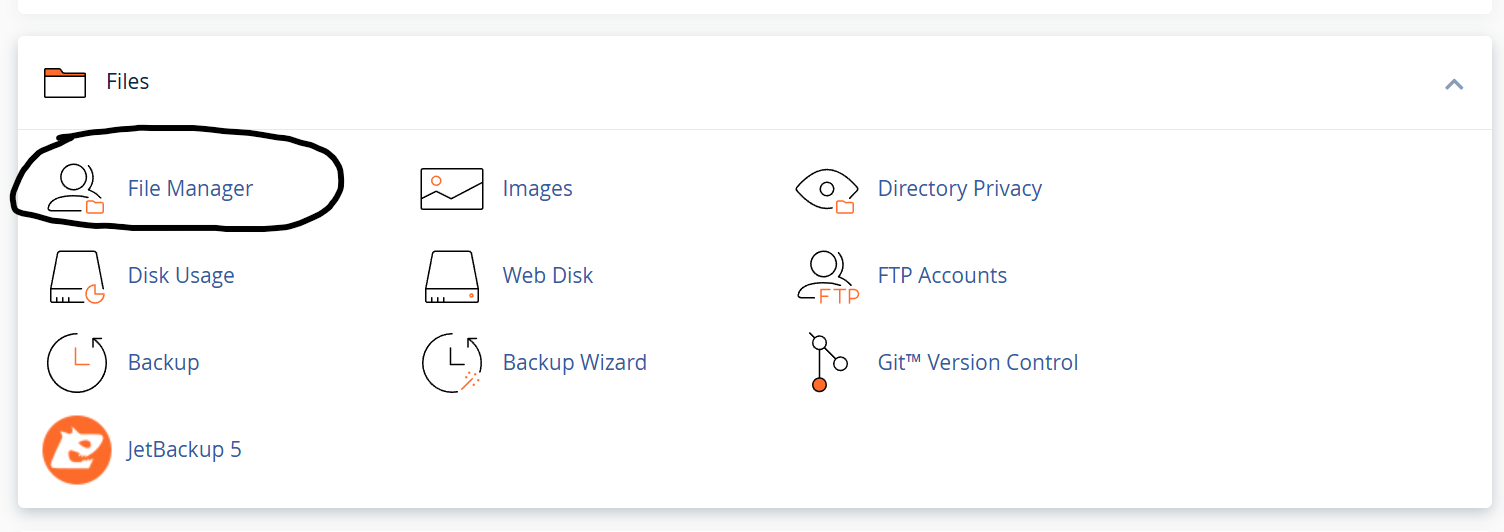
\includegraphics[width=10cm]{Gambar/bab3/instalasi-sistem-online/instalasi-sistem-online-tombol-file-manager.png}
    	\caption{Tombol \textit{Menu File Manager} Pada CPanel}
    	\label{fig:instalasi-sistem-online-tombol-menu-file-manager-pada-cpanel}
        \end{figure}
        \FloatBarrier
        \item Menekan tombol "\textit{Upload}" yang terdapat pada \textit{file manager} dan \textit{upload folder} aplikasi presensi \textit{online} yang telah di-\textit{zip} sebelumnya, serta melakukan \textit{extract} pada \textit{folder} tersebut. \textbf{\ref{fig:instalasi-sistem-online-tombol-tombol-upload-pada-file-manager}} menunjukkan tombol \textit{upload} pada \textit{file manager}.
        \begin{figure}[!htbp]
    	\centering
    	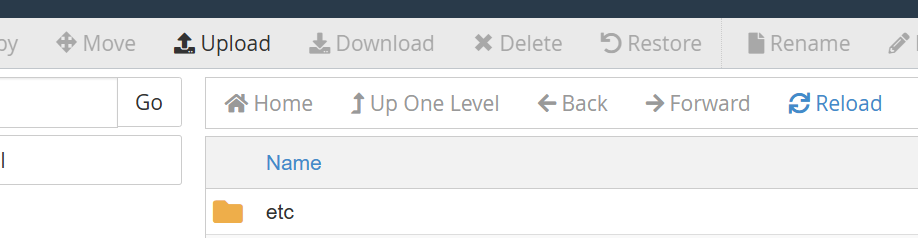
\includegraphics[width=10cm]{Gambar/bab3/instalasi-sistem-online/instalasi-sistem-online-tombol-upload-pada-file-manager.png}
    	\caption{Tombol Upload Pada \textit{File Manager}}
    	\label{fig:instalasi-sistem-online-tombol-tombol-upload-pada-file-manager}
        \end{figure}
        \FloatBarrier
    \end{enumerate}
    
    \item Memindahkan seluruh isi dari \textit{folder public} pada aplikasi presensi \textit{online} ke public\_html. \textbf{\ref{fig:instalasi-sistem-online-folder-public-html}} menunjukkan \textit{folder} public\_html pada \textit{file manager}.
    \begin{figure}[!htbp]
    	\centering
    	
\includegraphics[width=10cm]{Gambar/bab3/instalasi-sistem-online/instalasi-sistem-online-folder-public-html.png}
    	\caption{\textit{Folder} Public\_html Pada \textit{File Manager}}
    	\label{fig:instalasi-sistem-online-folder-public-html}
        \end{figure}
        \FloatBarrier

    \item Melakukan konfigurasi \textit{path} \textit{require} dan \textit{app} pada \textit{file} index.php yang terletak pada public\_html sebelumnya dengan nama \textit{folder} aplikasi presensi \textit{online}. \textbf{\ref{fig:instalasi-sistem-online-konfigurasi-file-index-php}} menunjukkan isi \textit{file} index.php yang telah dikonfigurasi.

    \begin{figure}[!htbp]
    	\centering
    	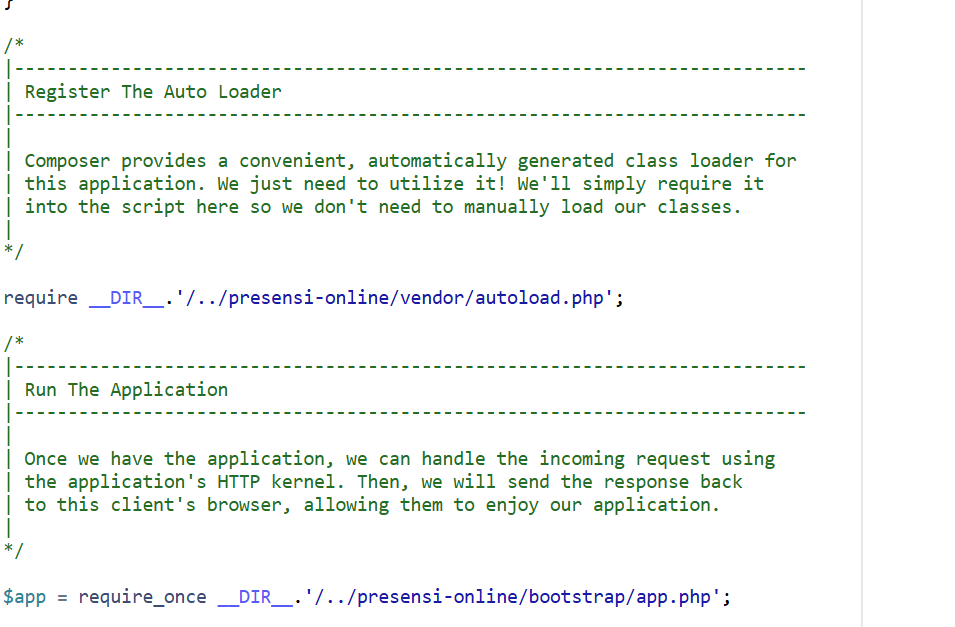
\includegraphics[width=10cm]{Gambar/bab3/instalasi-sistem-online/instalasi-sistem-online-konfigurasi-file-index-php.png}
    	\caption{Konfigurasi \textit{File} Index.php Pada Public\_html}
    	\label{fig:instalasi-sistem-online-konfigurasi-file-index-php}
        \end{figure}
        \FloatBarrier

    
    \item Melakukan konfigurasi pada \textit{file} .env untuk mengatur basis data dan mengatur \textit{email} yang akan digunakan untuk pengiriman kode OTP.
    
    \item Mengatur \textit{basis data} melalui menu PhpMyAdmin pada CPanel.
    \begin{enumerate}
        \item Menekan menu PHPMyAdmin pada CPanel. \textbf{\ref{fig:instalasi-sistem-online-tombol-phpmyadmin-pada-cpanel}} menunjukkan tombol PHPMyAdmin pada CPanel.
        \begin{figure}[!htbp]
    	\centering
    	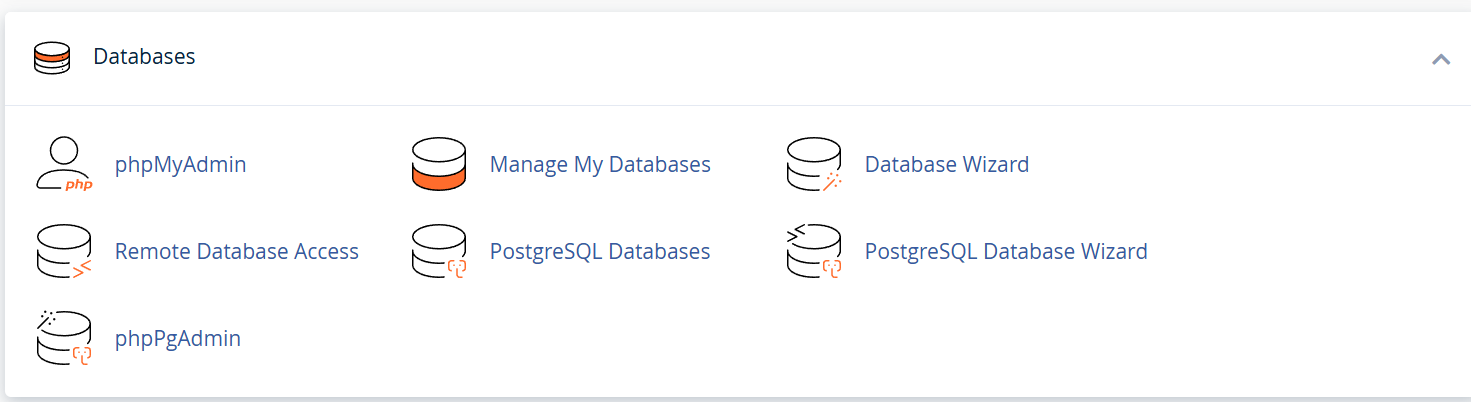
\includegraphics[width=10cm]{Gambar/bab3/instalasi-sistem-online/instalasi-sistem-online-tombol-phpmyadmin.png}
    	\caption{Tombol PHPMyAdmin Pada CPanel}
    	\label{fig:instalasi-sistem-online-tombol-phpmyadmin-pada-cpanel}
        \end{figure}
        \FloatBarrier
        \item Melakukan \textit{import file} .sql yang telah didapatkan melalui aplikasi presensi \textit{online} saat dijalankan secara lokal. \textbf{\ref{fig:instalasi-sistem-online-tombol-import-pada-cpanel}} menunjukkan tombol "\textit{Import}" pada PHPMyAdmin.
        \begin{figure}[!htbp]
    	\centering
    	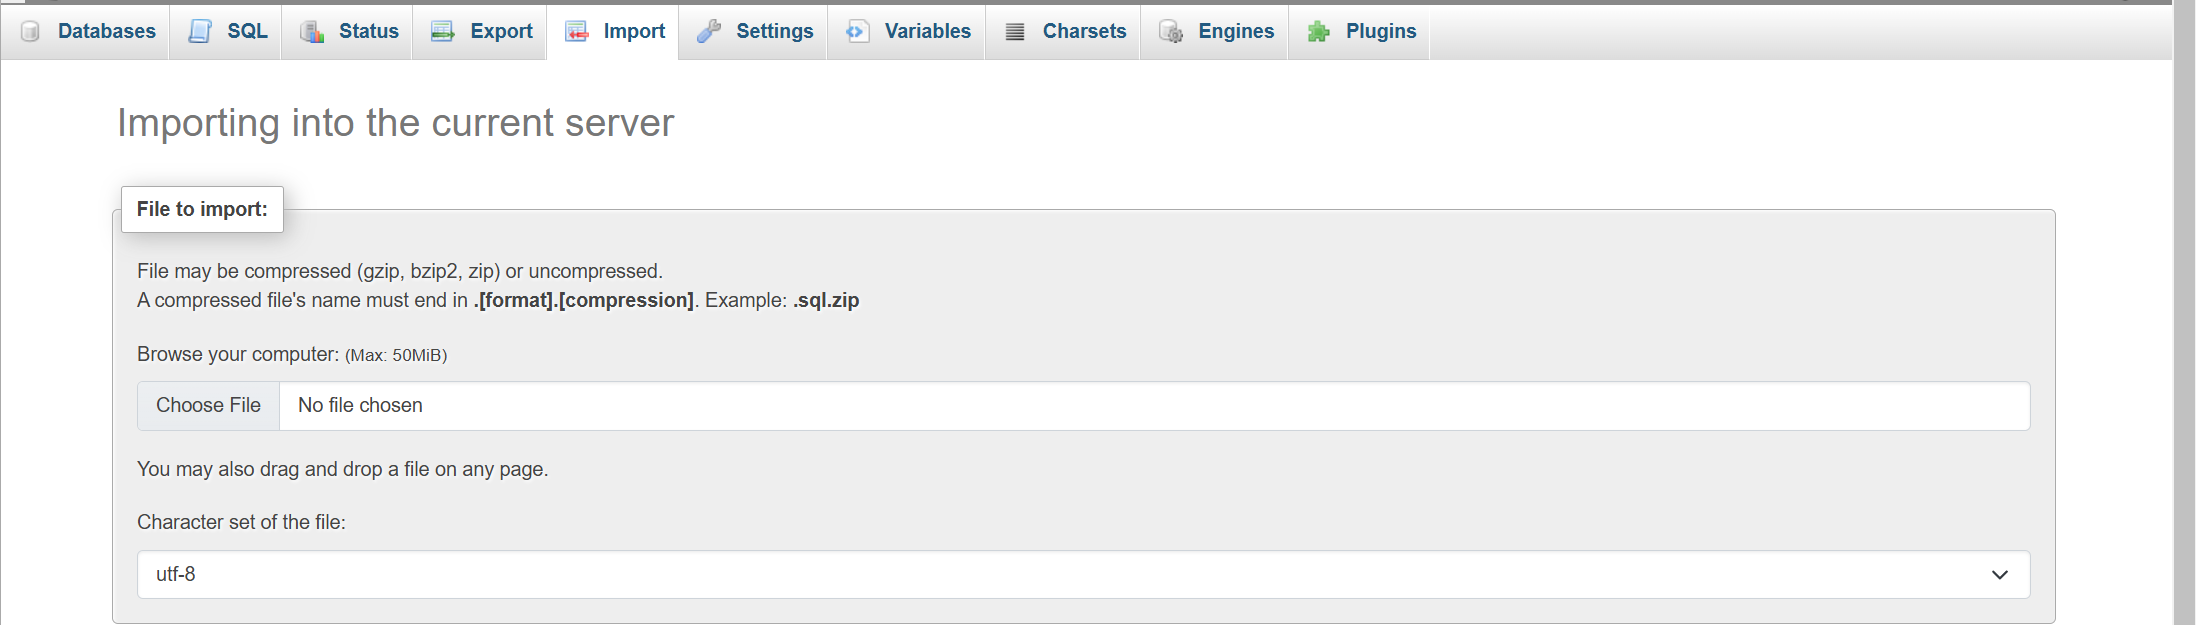
\includegraphics[width=10cm]{Gambar/bab3/instalasi-sistem-online/instalasi-sistem-online-tombol-import-phpmyadmin.png}
    	\caption{Tombol \textit{Import} Pada PHPMyAdmin}
    	\label{fig:instalasi-sistem-online-tombol-import-pada-cpanel}
        \end{figure}
        \FloatBarrier
    \end{enumerate}
    \item Melakukan instalasi SSL.
    \begin{enumerate}
        \item Menekan tombol menu \textit{"Let's Encrypt"} pada CPanel. \textbf{\ref{fig:instalasi-sistem-online-tombol-lets-encrypt}} menunjukkan tombol menu "\textit{Let's Encrypt}" pada CPanel.
        \begin{figure}[!htbp]
    	\centering
    	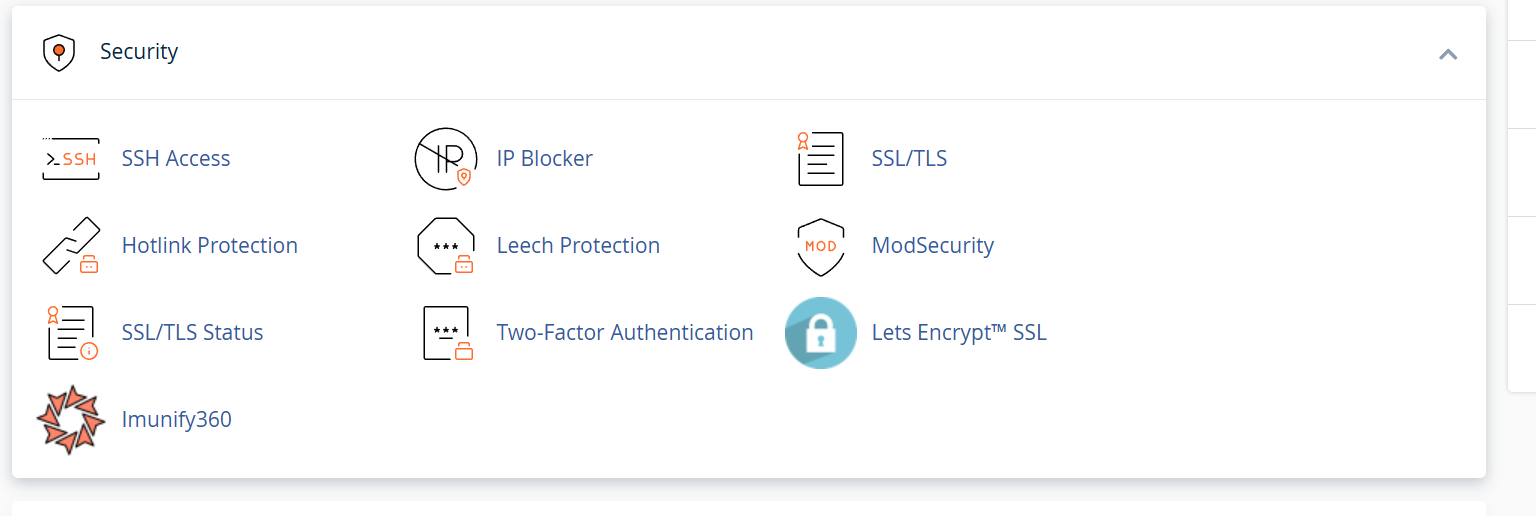
\includegraphics[width=10cm]{Gambar/bab3/instalasi-sistem-online/instalasi-sistem-online-tombol-lets-encrypt.png}
    	\caption{Tombol \textit{Let's Encrypt} Pada CPanel}
    	\label{fig:instalasi-sistem-online-tombol-lets-encrypt}
        \end{figure}
        \FloatBarrier
        \item Pada bagian \textit{Issue a new certificate}, tekan tombol "+ \textit{Issue}". \textbf{\ref{fig:instalasi-sistem-online-tombol-plus-issue-pada-lets-encrypt}} menunjukkan tombol "+ \textit{Issue}" pada bagian \textit{Issue a new certificate}.
        \begin{figure}[!htbp]
    	\centering
    	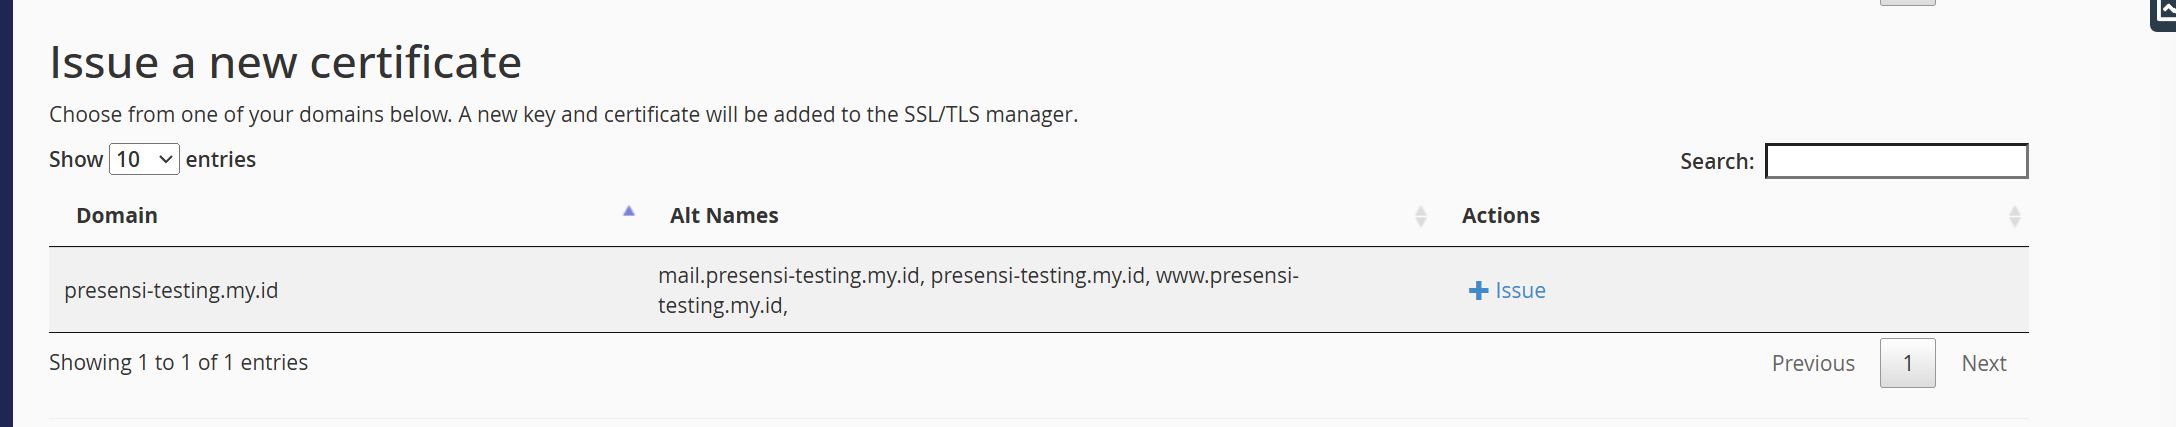
\includegraphics[width=10cm]{Gambar/bab3/instalasi-sistem-online/instalasi-sistem-online-tombol-issues-pada-lets-encrypt.png}
    	\caption{Tombol + \textit{Issue} Pada \textit{Let's Encrypt}}
    	\label{fig:instalasi-sistem-online-tombol-plus-issue-pada-lets-encrypt}
        \end{figure}
        \FloatBarrier
        \item pada bagian metode validasi SSL, pilih dns-01 dan tekan tombol "\textit{Issue}" untuk menyimpan metode yang dipilih. \textbf{\ref{fig:instalasi-sistem-online-tombol-dns01}} menunjukkan pilihan metode dns-01.
        \begin{figure}[!htbp]
    	\centering
    	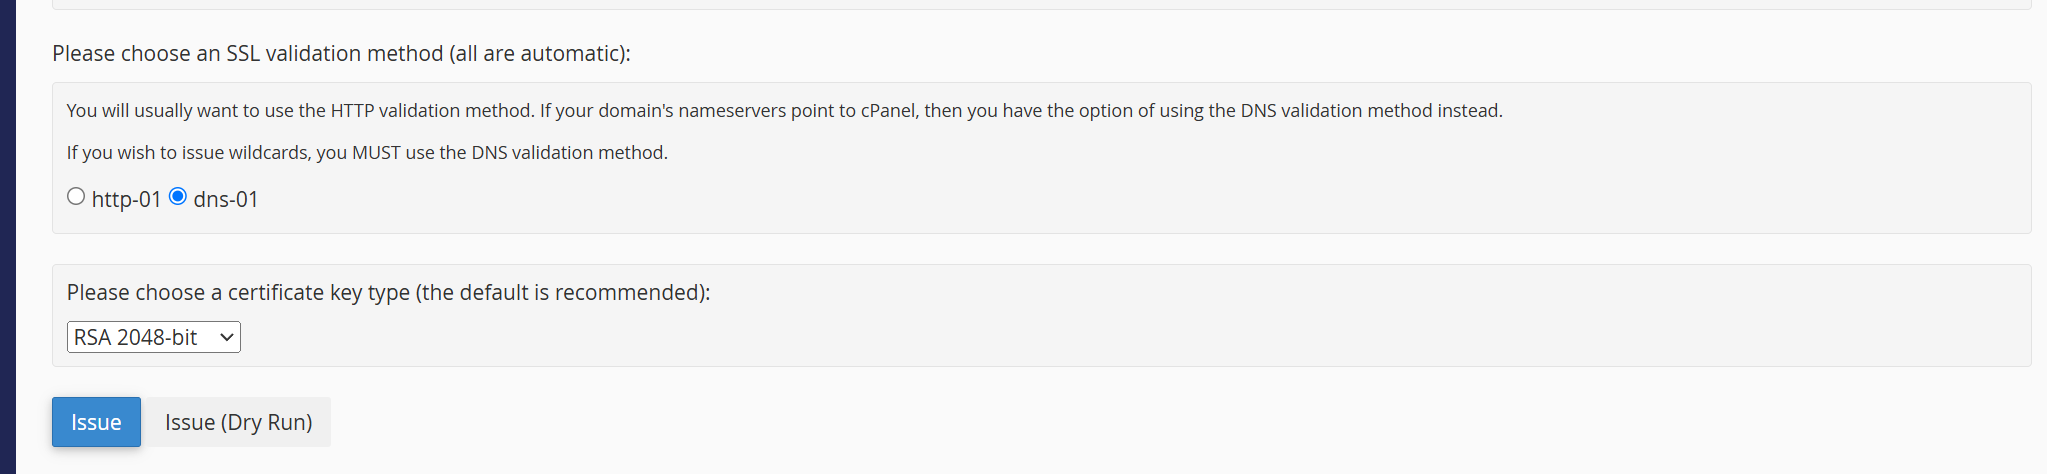
\includegraphics[width=10cm]{Gambar/bab3/instalasi-sistem-online/instalasi-sistem-online-tombol-dns01-pada-issues.png}
    	\caption{Metode Validasi SSL Dns-01}
    	\label{fig:instalasi-sistem-online-tombol-dns01}
        \end{figure}
        \FloatBarrier
    \end{enumerate}

\end{enumerate}

\subsection{\textit{User Manual}}
Terdapat \textit{user manual book} sebagai panduan untuk menggunakan aplikasi presensi \textit{online}. Pastikan telah melakukan instalasi sistem aplikasi secara lokal ataupun \textit{online} yang telah dilakukan pada \textbf{Subbab \ref{sec:instalation-system}} \textit{User manual book} dapat dilihat pada \textbf{\hyperref[sec:user-manual-aplikasi-presensi-online]{Lampiran~XII}}.


\section{Implementasi Sistem dan Jadwal}
Pada proses ini merupakan tahapan untuk mengimplementasikan sistem sesuai dengan perancangan proses dan peracangan antar muka yang telah dibuat sebelumnya. Tahap ini dimulai dari pembuatan \textit{database} dan penulisan kode program. Setelah itu akan dilakukan \textit{unit testing} yaitu pengujian yang dilakukan oleh pengembang aplikasi untuk memastikan seluruh fungsi dari aplikasi berjalan dengan semestinya. Kemudian, dilakukan UAT (\textit{User Acceptance Testing}) untuk memastikan fitur dari setiap aplikasi sudah sesuai dengan kebutuhan \textit{user}. Setelah pengujian, akan dilakukan \textit{deployment} pada \textit{website} dan pelatihan aplikasi kepada seluruh personil aplikasi yang dilakukan secara tatap muka. Jadwal implementasi sistem dapat dilihat pada \textbf{\hyperref[sec:gantt-chart-implementasi-sistem]{Lampiran~XIII}, \ref{fig:gantt-chart-implementasi-sistem}}.

\section{Perawatan Sistem dan Jadwal}
Setelah sistem diimplementasikan, pemeliharaan akan dilakukan setiap bulan untuk memastikan sistem berjalan dengan baik dan bebas dari masalah teknis. Proses ini meliputi deteksi dan perbaikan masalah yang mungkin muncul selama penggunaan. Pemeliharaan ini akan dilakukan setelah seluruh pengguna menerima pelatihan mendalam tentang cara kerja aplikasi dan fitur-fiturnya. Dengan pendekatan ini, tidak hanya memastikan sistem tetap berfungsi dengan baik, tetapi juga memastikan pengguna dapat memanfaatkan sistem dengan maksimal.

\chapter{HASIL PENGUJIAN DAN PEMBAHASAN}

\section{Pengujian}
Pengujian akan dilakukan dalam dua tahap, yaitu pengujian oleh \textit{programmer} untuk memastikan stabilitas sistem, dan pengujian oleh user yang melibatkan \textit{Staff Infrastructure}, \textit{Manager Infrastructure}, serta \textit{Manager Human Resources} di MyPassword, guna memastikan aplikasi sesuai kebutuhan pengguna.

\subsection{Pengujian Oleh \textit{Programmer}}
Pengujian oleh \textit{programmer} akan menggunakan metode \textit{whitebox testing}. \textit{Whitebox testing} merupakan teknik pengujian yang memeriksa struktur internal aplikasi. Pengujian ini berfokus pada struktur kode aplikasi, logika internal dan algoritma untuk menguji aplikasi. Tujuan \textit{whitebox testing} adalah menemukan kesalahan dalam struktur kode dan memastikan fungsi aplikasi berjalan dengan baik~\cite{introducion2023panagiotis}. Pengujian aplikasi presensi \textit{online} akan dilakukan pengujian pada seluruh fitur. Pengujian ini bertujuan untuk memastikan bahwa setiap fitur aplikasi dapat berfungsi optimal dan memberikan pengalaman pengguna yang konsisten. Hasil pengujian yang dilakukan oleh \textit{programmer} pada aplikasi presensi \textit{online} berbasis web menunjukkan hasil valid untuk seluruh kasus uji yang disusun, yang dapat dilihat pada \textbf{\hyperref[sec:whitebox-testing-aplikasi-presensi-online-oleh-programmer]{Lampiran~XIV}}. Berdasarkan hasil tersebut, aplikasi dinyatakan telah memenuhi standar kualitas dari sisi internal.

\subsection{Pengujian oleh User}
Pada pengujian oleh user, akan menggunakan metode \textit{blackbox testing}, yaitu pengujian yang dilakukan untuk mengamati hasil \textit{input} dan \textit{output} dari aplikasi tanpa mengetahui struktur kode dari aplikasi~\cite{introducion2023panagiotis}. Pengujian dilakukan oleh ketiga user yaitu Staff Infrastructure, Manager Infrastructure, dan Manager Human Resources pada tanggal 24 oktober 2024. Pengujian pertama dilakukan oleh Ibu Loren Cyntya selaku \textit{Staff Infrastructure} untuk memastikan tidak ada kesalahan pada fungsi dasar aplikasi seperti melakukan presensi, melakukan pengajuan lembur dan melihat riwayat presensi atau lembur. Hasil pengujian oleh \textit{Staff Infrastructure} dapat dilihat pada \textbf{\hyperref[sec:blackbox-testing-aplikasi-presensi-online-oleh-staff-infrastructure]{Lampiran~XV}}, dokumentasi pengujian oleh \textit{Staff Infrastructure} dapat dilihat pada \textbf{\hyperref[sec:dokumentasi-blackbox-testing]{Lampiran~XVIII}},\textbf{~\ref{fig:dokumentasi-blackbox-testing-oleh-staff-infrastructure}}. Selanjutnya, pengujian kedua dilakukan oleh Ibu Melissa selaku \textit{Manager Human Resources}, pengujian akan difokuskan pada fitur pengelolaan \textit{shift}, pengelolaan libur perusahaan, pengelolaan \textit{user}, \textit{export} data lembur dan \textit{export} data presensi. Hasil pengujian oleh \textit{Manager Human Resources} dapat dilihat pada \textbf{\hyperref[sec:blackbox-testing-aplikasi-presensi-online-oleh-manager-hrd]{Lampiran~XVI}}, dokumentasi pengujian oleh \textit{Manager Human Resources} dapat dilihat pada \textbf{\hyperref[sec:dokumentasi-blackbox-testing]{Lampiran~XVIII}},\textbf{~\ref{fig:dokumentasi-blackbox-testing-oleh-manager-human-resources}}. Terakhir, pengujian akan dilakukan oleh Bapak Imam Zaenuri selaku \textit{Manager Infrastructure}, fokus dari pengujian akan sama seperti fitur yang diuji oleh \textit{Manager Human Resources}, namun terdapat tambahan fitur yang akan diuji yaitu \textit{reject} pada data lembur. Hasil pengujian oleh \textit{Manager Infrastructure} dapat dilihat pada \textbf{\hyperref[sec:blackbox-testing-aplikasi-presensi-online-oleh-manager-infrastructure]{Lampiran~XVII}}, dokumentasi pengujian oleh \textit{Manager Infrastructure} dapat dilihat pada \textbf{\hyperref[sec:dokumentasi-blackbox-testing]{Lampiran~XVIII}},\textbf{~\ref{fig:dokumentasi-blackbox-testing-oleh-manager-infrastructure}}.

\subsection{Pengujian \textit{Geolocation}}
Pada pengujian \textit{Geolocation} akan dilakukan menggunakan \textit{browser} pada \textit{smartphone} yang memiliki GPS. Pada proses pengujian, pengambilan koordinat lokasi dan nama alamat akan dilakukan menggunakan \textit{Geolocation} API yang terintegrasi dalam aplikasi presensi \textit{online}. Titik koordinat dan nama alamat yang diperoleh dari hasil pengujian tersebut akan diverifikasi menggunakan \textit{Google Maps} untuk memastikan akurasi dan kesesuaian lokasi yang terdeteksi dengan lokasi sebenarnya. \textbf{\ref{tab:table-pengujian-geolocation}} menunjukkan tabel hasil pengujian \textit{geolocation} pada aplikasi presensi \textit{online}. Pengujian dilakukan pada 10 lokasi yang berbeda, seluruh hasil pengujian mendapatkan hasil yang sesuai terhadap titik lokasi yang diperoleh melalui \textit{Geolocation} API pada aplikasi presensi \textit{online} sehingga fitur \textit{Geolocation} pada aplikasi presensi \textit{online} memiliki akurasi yang baik untuk mendapatkan titik koordinat lokasi pada perangkat.

\begin{longtable}{ |p{0.5cm}|p{2cm}|p{2.5cm}|p{6cm}|p{1cm}|}
\caption{Tabel Pengujian \textit{Geolocation}}\label{tab:table-pengujian-geolocation} 
\\
\hline
\textbf{No}
&\textbf{Nama Tempat}
&\textbf{Titik Koordinat}
&\textbf{Nama Alamat}
&\textbf{Hasil Uji}
\\ 
\hline

\multirow{1}{*}{1}
&MyPassword
&-6.190578, 106.7978118
&Wisma 77 Slipi, 77, Jalan Letnan Jenderal Siswondo Parman, RW 03, Slipi, Palmerah, West Jakarta, Special capital Region of Jakarta, Java, 11420, Indonesia
&Sesuai
\\
\hline

\multirow{1}{*}{2}
&Universitas Jakarta Internasional
&-6.1812963, 106.7963873
&Jalan Letnan Jenderal Siswondo Parman, RW 01, Kemanggisan, Palmerah, West Jakarta, Special capital Region of Jakarta, Java, 11420, Indonesia
&Sesuai
\\
\hline

\multirow{1}{*}{3}
&Mal Ciputra
&-6.1683184, 106.7873051
&Jalan Daan Mogot I, RW 01, Tanjung Duren Utara, Grogol Petamburan, West Jakarta, Special capital Region of Jakarta, Java, 11470, Indonesia
&Sesuai
\\
\hline

\multirow{1}{*}{4}
&Apotek Nusantara Sehat
&-6.1434918, 106.7931933
&Jalan Profesor Dokter Latumeten, RW 09, Angke, Tambora, West Jakarta, Special capital Region of Jakarta, Java, 11330, Indonesia
&Sesuai
\\
\hline

\multirow{1}{*}{5}
&Alfamart Lempuk
&-6.1310003, 106.7768492
&Jalan Lempuk, RW 13, Pejagalan, Penjaringan, North Jakarta, Special capital Region of Jakarta, Java, 14450, Indonesia
&Sesuai
\\
\hline

\multirow{1}{*}{6}
&Apatemen Teluk Intan
&-6.1286313, 106.77804
&Jalan Moa, RW 13, Pejagalan, Penjaringan, North Jakarta, Special capital Region of Jakarta, Java, 14450, Indonesia
&Sesuai
\\
\hline

\multirow{1}{*}{7}
&Season City
&-6.1520494, 106.7952633
&RW 05, Jembatan Besi, Tambora, West Jakarta, Special capital Region of Jakarta, Java, 11320, Indonesia
&Sesuai
\\
\hline

\multirow{1}{*}{8}
&Universitas Tarumanagara
&-6.1720398, 106.7897299
&Jalan Taman S. Parman, RW 16, Tomang, Grogol Petamburan, West Jakarta, Special capital Region of Jakarta, Java, 11450, Indonesia
&Sesuai
\\
\hline

\multirow{1}{*}{9}
&Hariston Hotel
&-6.1377053, 106.7879378
&Jalan Teluk Gong Raya, RW 16, Pejagalan, Penjaringan, North Jakarta, Special capital Region of Jakarta, Java, 14450, Indonesia
&Sesuai
\\
\hline

\multirow{1}{*}{10}
&Vihara Satria Dharma
&-6.138157, 106.786245
&Jalan Teluk Gong Raya, RW 09, Pejagalan, Penjaringan, North Jakarta, Special capital Region of Jakarta, Java, 14450, Indonesia
&Sesuai
\\
\hline


\end{longtable}

\subsection{Pengujian Perhitungan Jarak}
Pengujian perhitungan jarak akan membandingkan hasil perhitungan \textit{function} Haversine pada program aplikasi akan dibandingkan dengan perhitungan dari \textit{Google Geometry Library} API. \textit{Google} menyediakan API agar dapat menghitung jarak antara dua lokasi yang dapat diakses melalui tautan \url{https://developers.google.com/maps/documentation/javascript/geometry}. API ini disediakan dengan harga kurang lebih 1000 \textit{requests} sekitar Rp. 100.000 per bulan. \textbf{~\ref{fig:kode-google-geometry-library-api}} menampilkan contoh kode untuk melakukan permintaan \textit{request} kepada API \textit{Google} untuk perhitungan jarak. Selanjutnya, penulis akan melakukan perbandingan perhitungan jarak lokasi kantor MyPassword dengan 20 lokasi lainnya menggunakan algoritma Haversine pada program dengan \textit{Google Geometry Library} API. \textbf{~\ref{tab:table-perbandingan-haversine-dan-google}} menunjukkan tabel perbandingan menggunakan Haversine pada aplikasi presensi dengan \textit{Google Geometry Library} API pada 20 titik lokasi yang berbeda.
%
    \begin{figure}[!htbp]
    	\centering
    	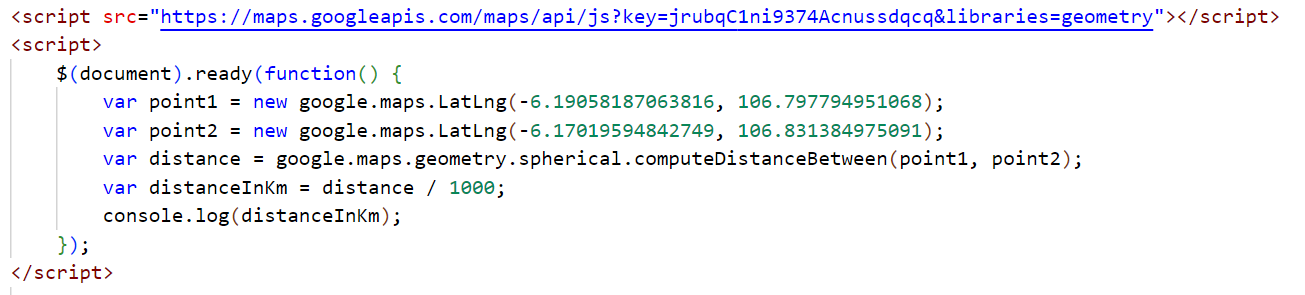
\includegraphics[width=13cm]{Gambar/bab3/google-geometry-library-api.png}
    	\caption{Kode Perhitungan Jarak \textit{Google Geometry Library} API}
    	\label{fig:kode-google-geometry-library-api}
    \end{figure}
    \FloatBarrier
%
\begin{longtable}{ |p{1cm}|p{3cm}|p{3cm}|p{3cm}|}
\caption{Tabel Perbandingan Algoritma Haversine Dengan \textit{Google Geometry Library} API}\label{tab:table-perbandingan-haversine-dan-google} 
\\
\hline
\textbf{No}
&\textbf{Lokasi}
&\textbf{Haversine Aplikasi Presensi (km)}
&\textbf{\textit{Google Geometry Library} (km)}
\\ 
\hline

\multirow{1}{*}{1}
&Universitas Tarumanagara
&2,5722
&2,5751
\\
\hline

\multirow{1}{*}{2}
&Gelora Bung Karno Stadium
&3,1518
&3,1554
\\
\hline

\multirow{1}{*}{3}
&Pasar Pecinan Glodok
&5,1614
&5,6212
\\
\hline

\multirow{1}{*}{4}
&Plaza Slipi Jaya
&0,2037
&0,2039
\\
\hline

\multirow{1}{*}{5}
&Pusat Jantung Nasional Harapan Kita
&0,5641
&0,5648
\\
\hline

\multirow{1}{*}{6}
&PIK Avenue
&11,0976
&11,1101
\\
\hline

\multirow{1}{*}{7}
&Thamrin City
&2,0578
&2,0602
\\
\hline

\multirow{1}{*}{8}
&Emporium Pluit
&7,0793
&7,0872
\\
\hline

\multirow{1}{*}{9}
&Apartemen Menteng Park
&4,6889
&4,6942
\\
\hline

\multirow{1}{*}{10}
&Central Park Mall
&1,5186
&1,5203
\\
\hline

\multirow{1}{*}{11}
&Summarecon Mall Serpong
&19,4990
&19,5208
\\
\hline

\multirow{1}{*}{12}
&Vihara Mahavira Graha Pusat
&7,3706
&7,3788
\\
\hline

\multirow{1}{*}{13}
&Stadium Patriot Candrabhaga
&22,1059
&22,1307
\\
\hline

\multirow{1}{*}{14}
&Pondok Zidane
&27,1100
&27,1404
\\
\hline

\multirow{1}{*}{15}
&Universitas Indonesia
&19,1874
&19.2089
\\
\hline

\multirow{1}{*}{16}
&Grand Galaxy Park
&21,2442
&21,2680
\\
\hline

\multirow{1}{*}{17}
&Museum Pancasila Sakti
&16,4728
&16,4913
\\
\hline

\multirow{1}{*}{18}
&Aeon Mall BSD City
&21,3194
&21,3433
\\
\hline

\multirow{1}{*}{19}
&Sarinah
&2,8680
&2,8712
\\
\hline

\multirow{1}{*}{20}
&Masjid Istiqlal
&4,3505
&4,3554
\\
\hline

\multirow{1}{*}{}
&\textbf{Rata-Rata}
&\textbf{10,0038}
&\textbf{10,0151}
\\
\hline

\end{longtable}

Hasil perhitungan rata-rata dari 20 koordinat lokasi yang dibandingkan dengan koordinat kantor MyPassword menggunakan Algoritma Haversine pada aplikasi presensi menunjukkan hasil 10,0038. Namun, ketika dibandingkan dengan hasil perhitungan menggunakan \textit{Google Geometry Library}, yang memiliki rata-rata 10,0151, terdapat perbedaan sebesar 0,0113. Hal ini menunjukkan adanya sedikit perbedaan antara hasil perhitungan Algoritma Haversine pada aplikasi dan \textit{Google Geometry Library}, namun selisih tersebut masih dalam batas toleransi yang dapat diterima untuk sebagian besar aplikasi praktis, termasuk aplikasi presensi.

\subsection{Pengujian Perhitungan Lembur}
Pada pengujian perhitungan lembur akan dilakukan beberapa skenario \textit{test case} untuk memastikan bahwa fitur perhitungan lembur dapat membuat dan menghitung data lembur secara otomatis jika \textit{Staff Infrastructure} melakukan presensi diluar penjadwalan \textit{shift} atau pada hari libur perusahaan. Sebelum melakukan pengujian akan terdapat beberapa konfigurasi yang dilakukan. Mengatur jenis shift yang terdiri dari hari Senin hingga Jumat mulai pukul 8 pagi hingga 5 sore dan hari Sabtu mulai pukul 8 pagi hingga 12 siang. \textbf{\ref{fig:pengaturan-jenis-shift}} menunjukkan hasil pengaturan hari pada jenis \textit{shift}.
\begin{figure}[!htbp]
    	\centering
    	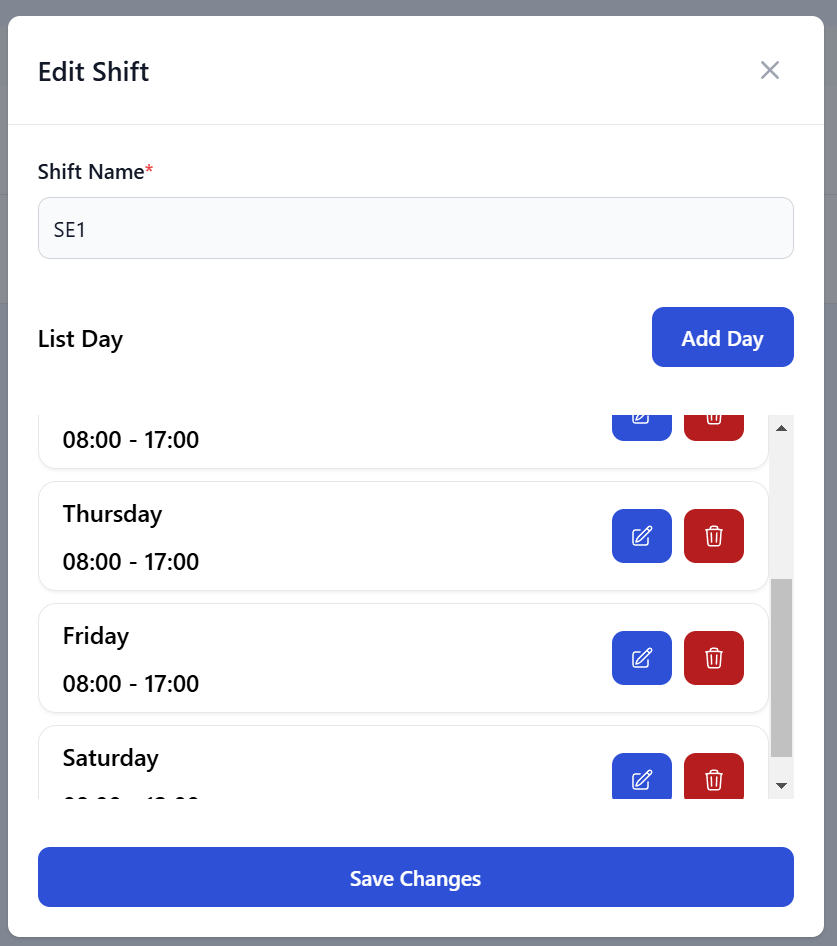
\includegraphics[width=9cm]{Gambar/bab4/pengaturan-jenis-shift.png}
    	\caption{Pengaturan Jenis \textit{Shift}}
    	\label{fig:pengaturan-jenis-shift}
        \end{figure}
        \FloatBarrier

Selanjutnya, menjadwalkan penggunaan jenis \textit{shift} yang telah dibuat sebelumnya dengan akun yang akan digunakan untuk pengujian. Jenis \textit{shift} akan dijadwalkan mulai tanggal 1 Januari 2024 hingga 31 Desember 2024. Hasil pengaturan penjadwalan \textit{shift} dapat dilihat pada \textbf{\ref{fig:pengaturan-penjadwalan-shift}}.
\begin{figure}[!htbp]
    	\centering
    	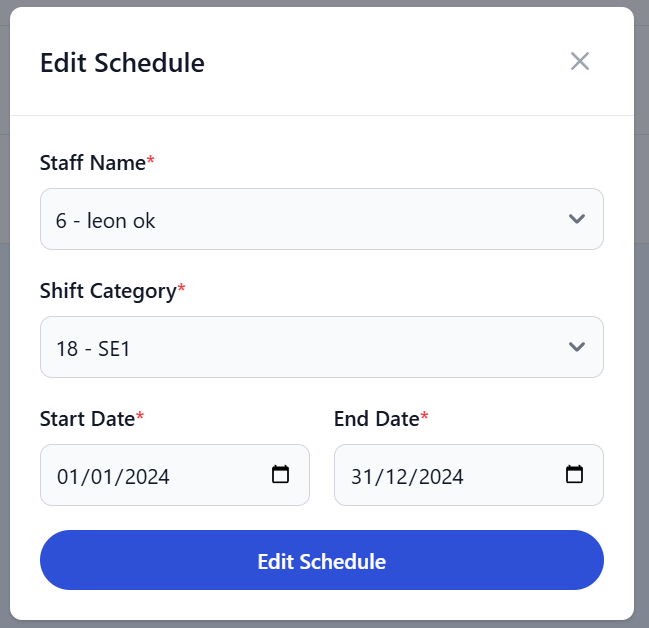
\includegraphics[width=9cm]{Gambar/bab4/pengaturan-penjadwalan-shift.png}
    	\caption{Pengaturan Penjadwalan \textit{Shift}}
    	\label{fig:pengaturan-penjadwalan-shift}
        \end{figure}
        \FloatBarrier

Setelah itu, membuat jenis libur baru yang berisi hari libur nasional Indonesia tahun 2024, penulis juga menambah libur pada tanggal 14 Desember 2024 sebagai pengujian. Hasil pembuatan jenis libur dapat dilihat pada \textbf{\ref{fig:pengujian-pengaturan-jenis-libur}}.
\begin{figure}[!htbp]
    	\centering
    	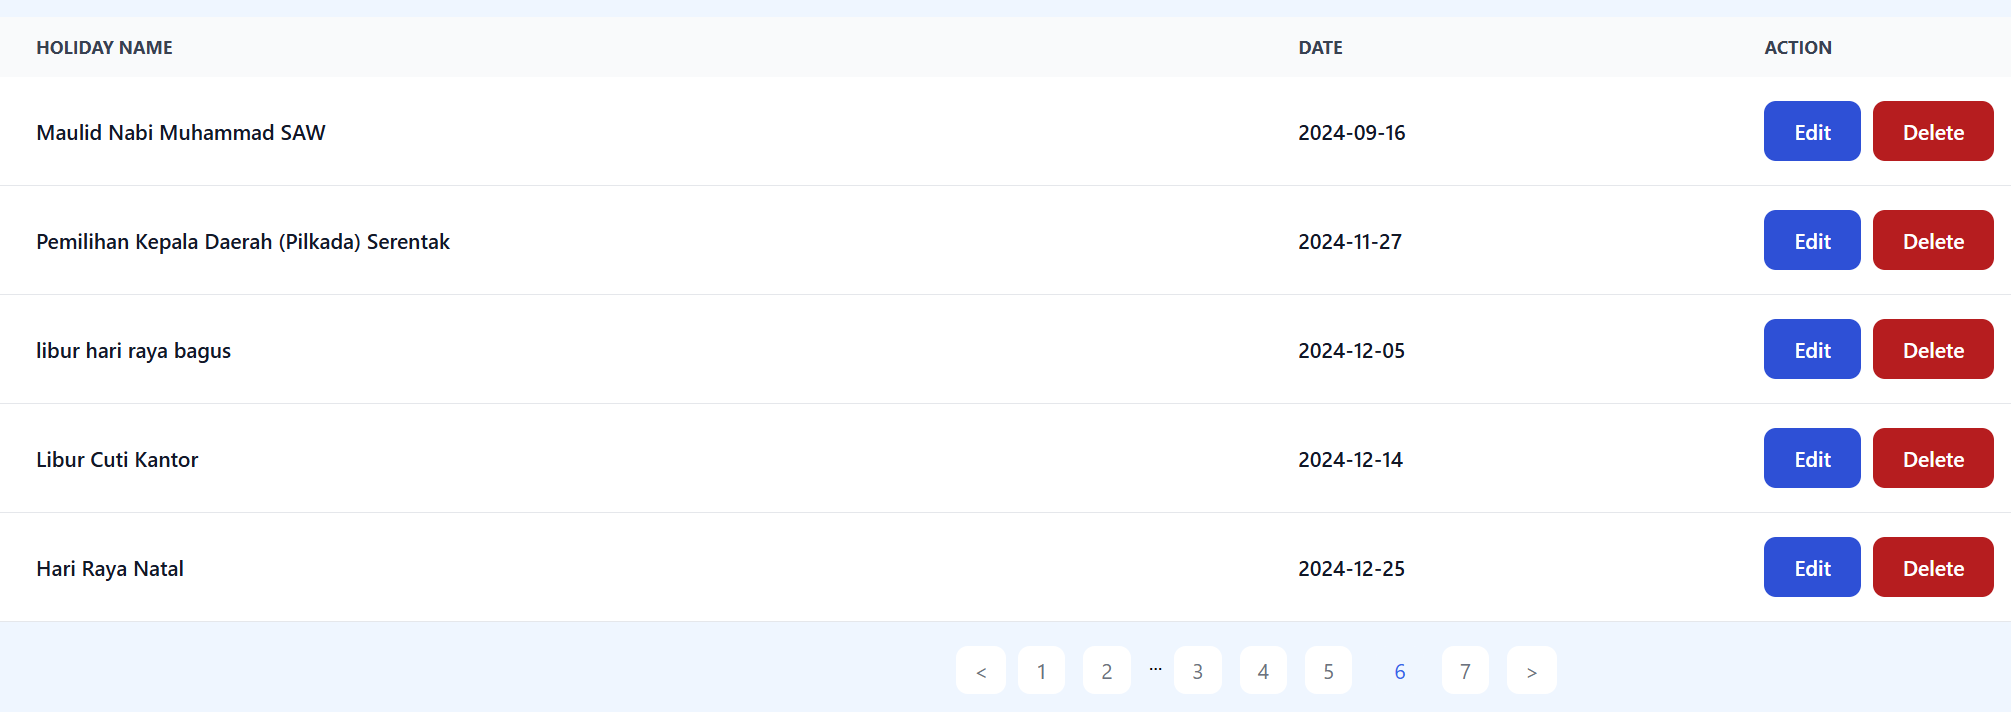
\includegraphics[width=17cm]{Gambar/bab4/pengaturan-jenis-libur.png}
    	\caption{Pengaturan Jenis Libur}
    	\label{fig:pengujian-pengaturan-jenis-libur}
        \end{figure}
        \FloatBarrier

Selanjtunya, menghubungkan akun yang akan digunakan sebagai pengujian dengan jenis libur yang telah dibuat sebelumnya melalui pengaturan \textit{user}. \textbf{\ref{fig:pengaturan-akun-user-dengan-jenis-libur}} menunjukkan hasil dari menghubungkan akun yang akan digunakan sebagai pengujian dengan jenis libur yang telah dibuat sebelumnya.
\begin{figure}[!htbp]
    	\centering
    	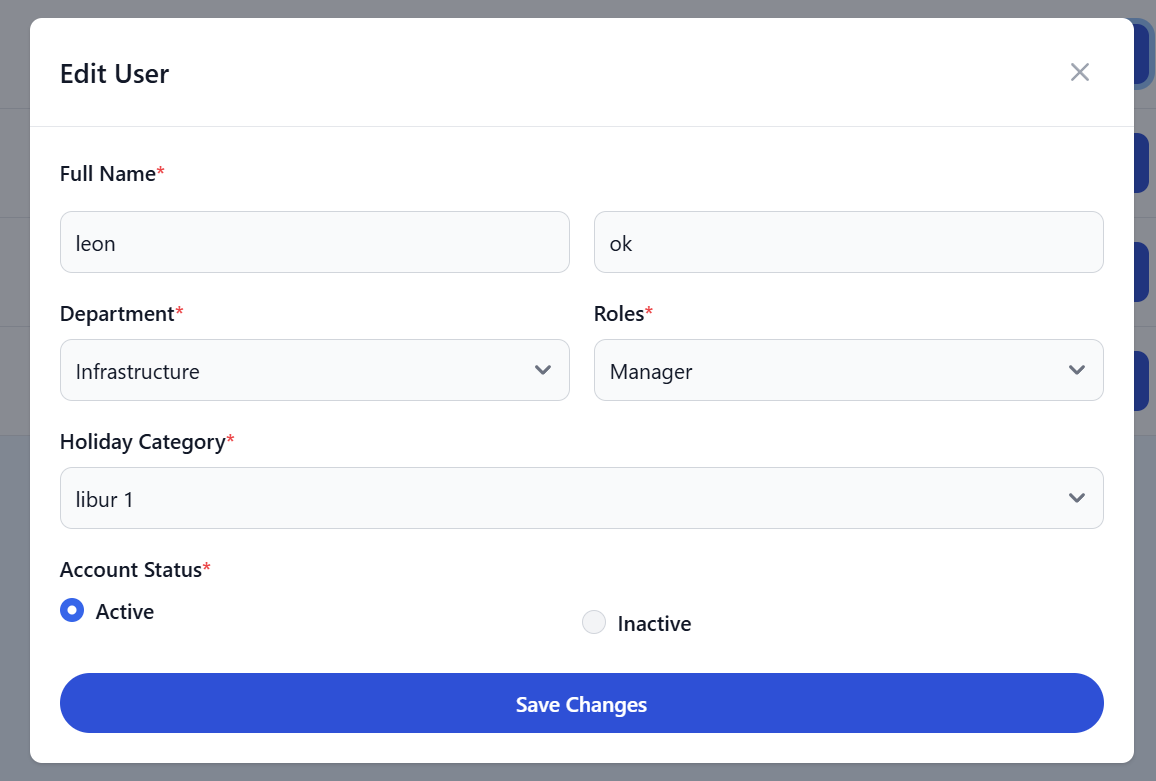
\includegraphics[width=9cm]{Gambar/bab4/pengaturan-pengaturan-user-libur.png}
    	\caption{Pengaturan Akun \textit{User} dengan Jenis Libur}
    	\label{fig:pengaturan-akun-user-dengan-jenis-libur}
        \end{figure}
        \FloatBarrier

Setelah \textit{shift} dan libur sudah dikonfigurasi, penulis melakukan pengujian pada skenario pertama yaitu melakukan presensi masuk pada hari Senin tanggal 12 Desember 2024 pukul 07.00 dan melakukan presensi keluar pada hari yang sama pukul 22.32. \textbf{\ref{fig:hasil-riwayat-presensi-skenario-pertama}} menunjukkan hasil riwayat presensi pada skenario pertama.
\begin{figure}[!htbp]
    	\centering
    	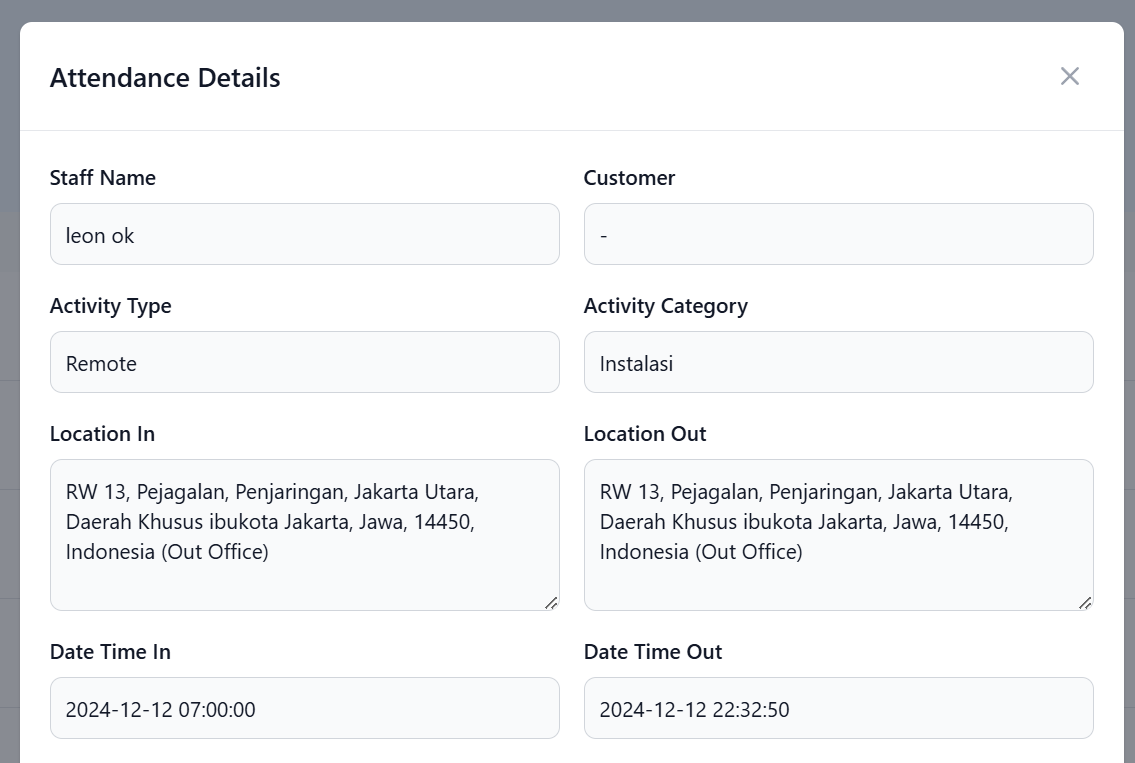
\includegraphics[width=9cm]{Gambar/bab4/pengujian-lembur-otomatis-attendance-1.png}
    	\caption{Hasil Riwayat Presensi Skenario Pertama}
    	\label{fig:hasil-riwayat-presensi-skenario-pertama}
        \end{figure}
        \FloatBarrier

Pada skenario pertama, sistem berhasil mendeteksi adanya lembur karena presensi masuk dilakukan sebelum \textit{shift} masuk dan presensi keluar dilakukan setelah \textit{shift} selesai. Sistem juga otomatis menghitung total jam lembur yaitu 6 jam 32 menit. Hasil riwayat lembur skenario pertama dapat dilihat pada \textbf{\ref{fig:hasil-riwayat-lembur-skenario-pertama}}.
\begin{figure}[!htbp]
    	\centering
    	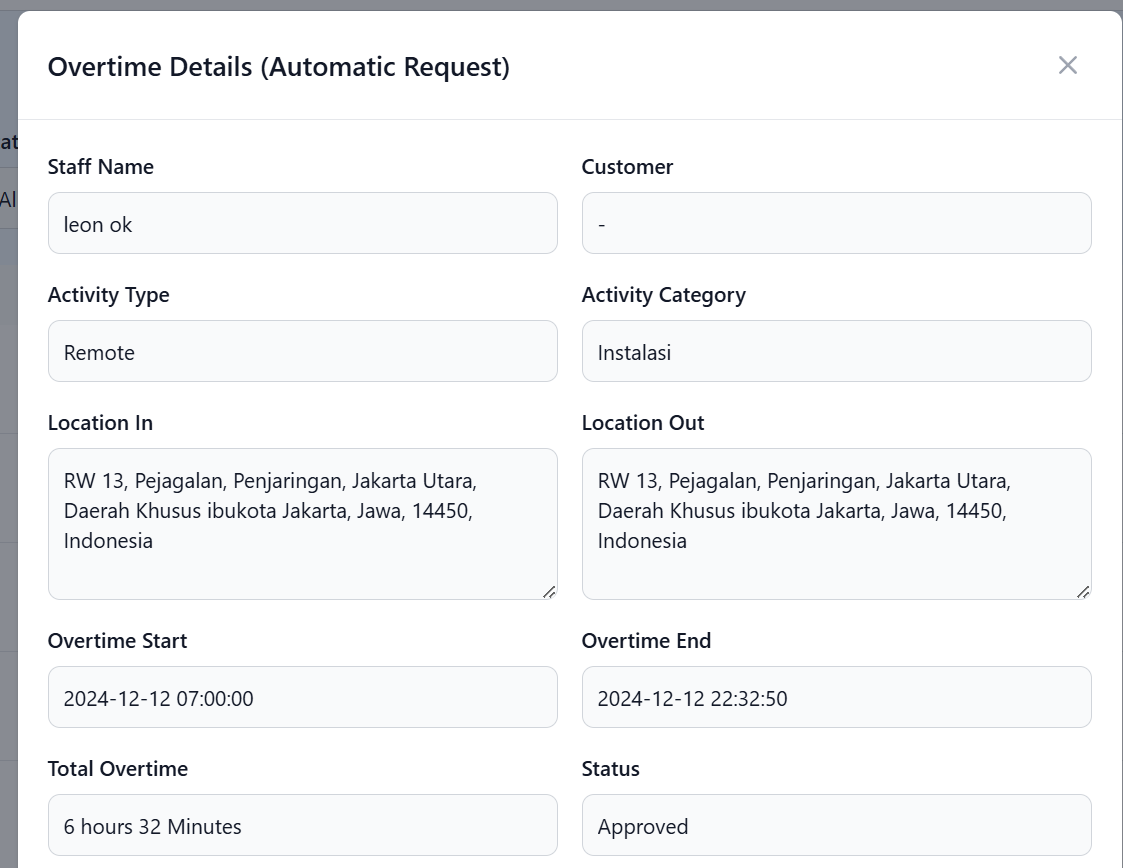
\includegraphics[width=9cm]{Gambar/bab4/pengujian-lembur-otomatis-overtime-1.png}
    	\caption{Hasil Riwayat Lembur Skenario Pertama}
    	\label{fig:hasil-riwayat-lembur-skenario-pertama}
        \end{figure}
        \FloatBarrier

Selanjutnya, pengujian skenario kedua dilakukan dengan melakukan presensi pada hari Senin tanggal 12 Desember 2024 pukul 17.30 dan presensi keluar pada hari yang sama pada pukul 22.27. Hasil riwayat presensi pada skenario kedua dapat dilihat pada \textbf{\ref{fig:hasil-riwayat-presensi-skenario-kedua}}.
\begin{figure}[!htbp]
    	\centering
    	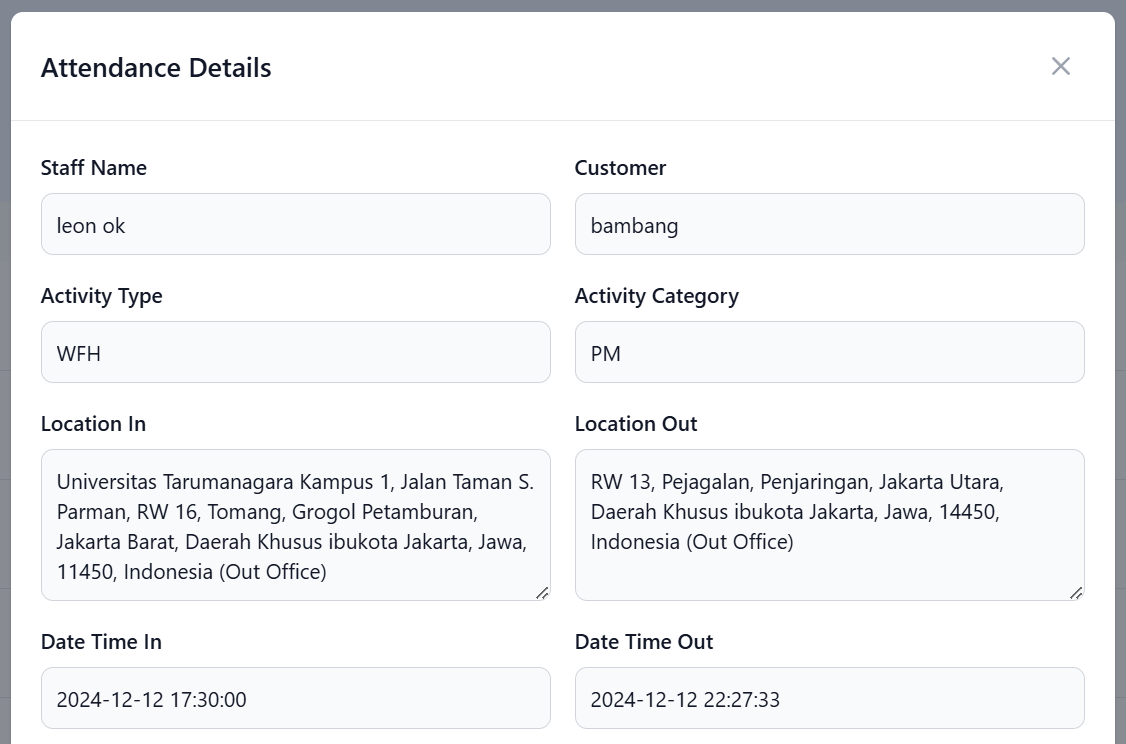
\includegraphics[width=9cm]{Gambar/bab4/pengujian-lembur-otomatis-attendance-2.png}
    	\caption{Hasil Riwayat Presensi Skenario Kedua}
    	\label{fig:hasil-riwayat-presensi-skenario-kedua}
        \end{figure}
        \FloatBarrier

Pada pengujian skenario kedua mendapatkan hasil yang sesuai. Sistem berhasil mendeteksi adanya lembur karena presensi masuk dan keluar dilakukan setelah \textit{shift} selesai. Sistem juga menghitung total jam lembur dengan hasil yang sesuai yaitu 4 jam 57 menit. Hasil riwayat lembur skenario kedua dapat dilihat pada \textbf{\ref{fig:hasil-riwayat-lembur-skenario-kedua}}.
\begin{figure}[!htbp]
    	\centering
    	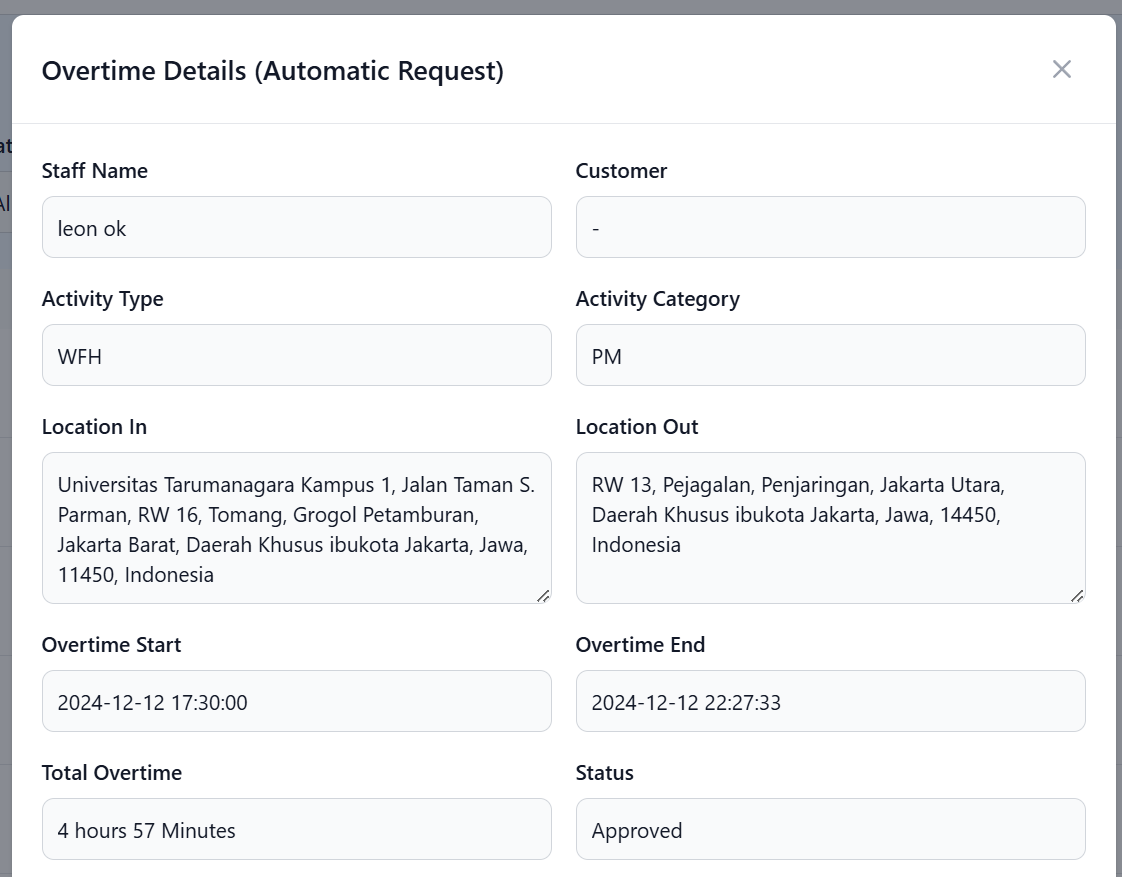
\includegraphics[width=9cm]{Gambar/bab4/pengujian-lembur-otomatis-overtime-2.png}
    	\caption{Hasil Riwayat Lembur Skenario Kedua}
    	\label{fig:hasil-riwayat-lembur-skenario-kedua}
        \end{figure}
        \FloatBarrier

Selanjutnya, pengujian pada skenario ketiga dilakukan dengan melakukan presensi masuk pada hari Senin tanggal 12 Desember 2024 pukul 22.33 dan presensi keluar pada hari yang berbeda yaitu Selasa tanggal 13 Desember 2024 pukul 09.46. Hasil riwayat presensi pada skenario ketiga dapat dilihat pada \textbf{\ref{fig:hasil-riwayat-presensi-skenario-ketiga}}.
\begin{figure}[!htbp]
    	\centering
    	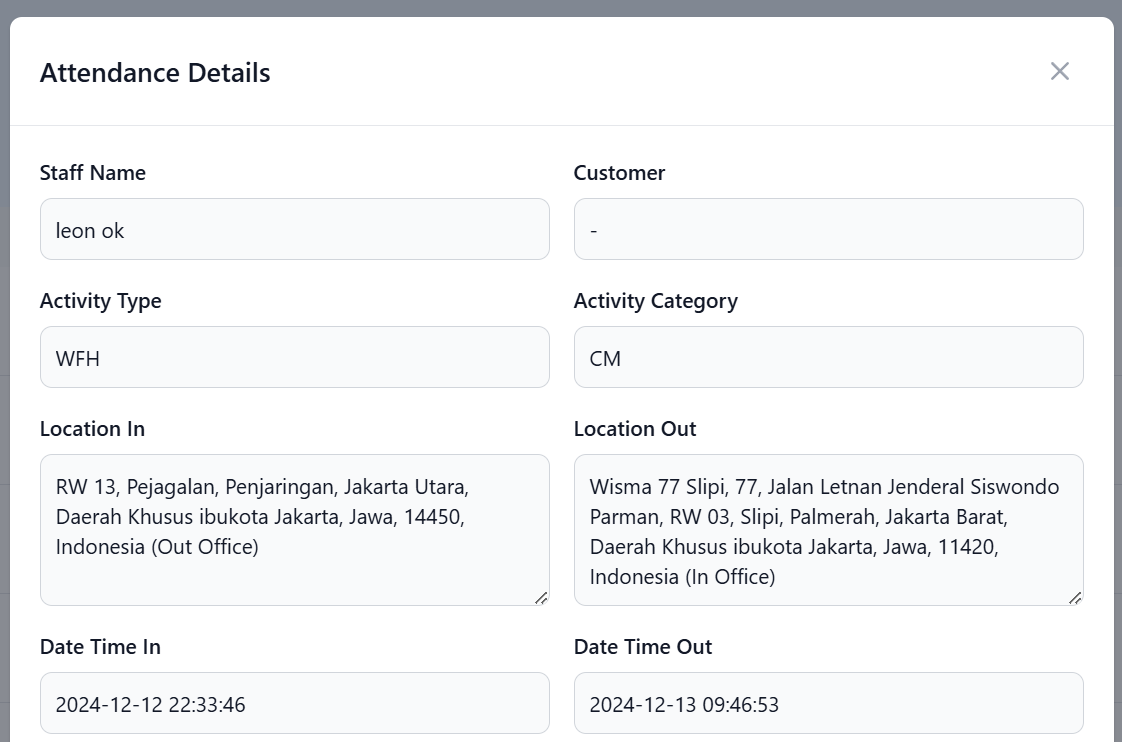
\includegraphics[width=9cm]{Gambar/bab4/pengujian-lembur-otomatis-attendance-3.png}
    	\caption{Hasil Riwayat Presensi Skenario Ketiga}
    	\label{fig:hasil-riwayat-presensi-skenario-ketiga}
        \end{figure}
        \FloatBarrier

Pada pengujian skenario ketiga, sistem berhasil mendeteksi adanya lembur karena presensi masuk dan keluar dilakukan setelah \textit{shift} selesai. Perhitungan total lembur juga sesuai walaupun presensi keluar dilakukan pada hari yang berbeda yaitu 9 jam 26 menit. Hasil riwayat lembur skenario ketiga dapat dilihat pada \textbf{\ref{fig:hasil-riwayat-lembur-skenario-ketiga}}.
\begin{figure}[!htbp]
    	\centering
    	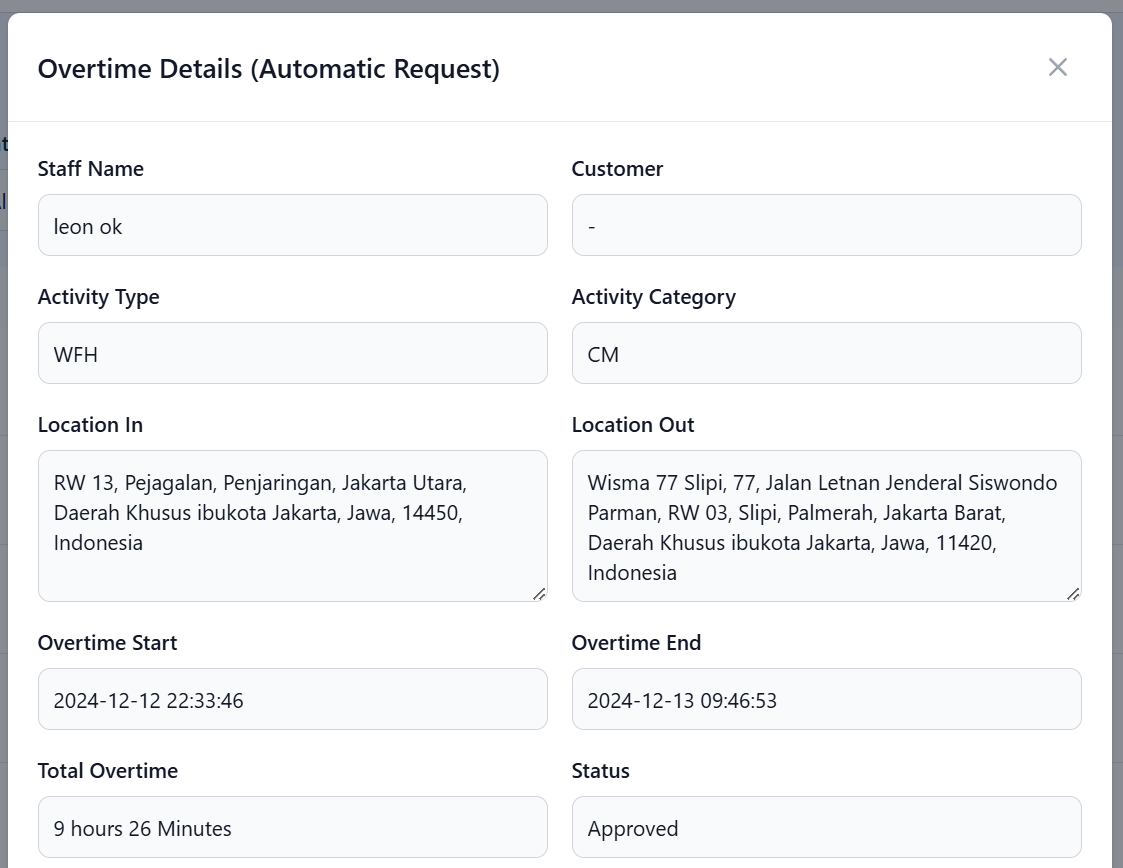
\includegraphics[width=9cm]{Gambar/bab4/pengujian-lembur-otomatis-overtime-3.png}
    	\caption{Hasil Riwayat Lembur Skenario Ketiga}
    	\label{fig:hasil-riwayat-lembur-skenario-ketiga}
        \end{figure}
        \FloatBarrier

Selanjutnya, pengujian pada skenario keempat dilakukan dengan melakukan presensi pada hari Selasa tanggal 13 Desember 2024 pukul 06.30 dan presensi keluar pada hari yang sama pukul 11.26. Hasil riwayat presensi pada skenario keempat dapat dilihat pada \textbf{\ref{fig:hasil-riwayat-presensi-skenario-keempat}}.
\begin{figure}[!htbp]
    	\centering
    	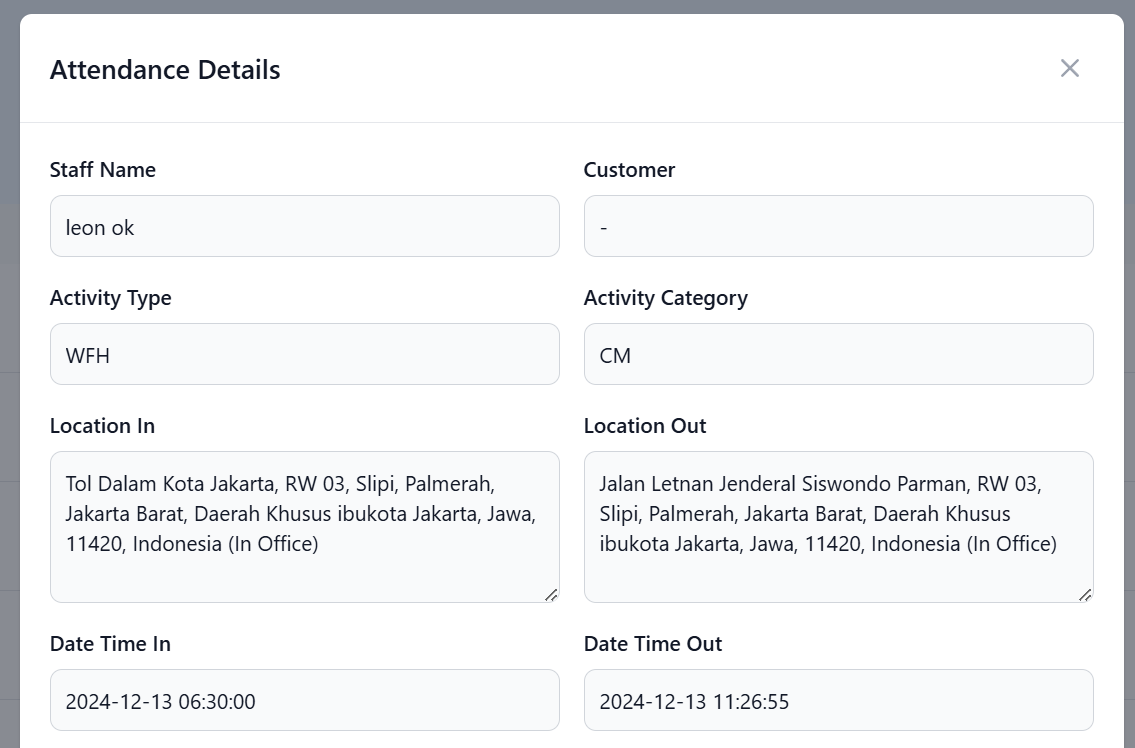
\includegraphics[width=9cm]{Gambar/bab4/pengujian-lembur-otomatis-attendance-4.png}
    	\caption{Hasil Riwayat Presensi Skenario Keempat}
    	\label{fig:hasil-riwayat-presensi-skenario-keempat}
        \end{figure}
        \FloatBarrier

Pada pengujian skenario keempat, sistem berhasil mendeteksi adanya lembur karena presensi masuk dilakukan sebelum \textit{shift} mulai. Sistem juga menghitung total lembur dengan hasil yang sesuai yaitu 1 jam 30 menit. Hasil riwayat lembur skenario keempat dapat dilihat pada \textbf{\ref{fig:hasil-riwayat-lembur-skenario-keempat}}.
\begin{figure}[!htbp]
    	\centering
    	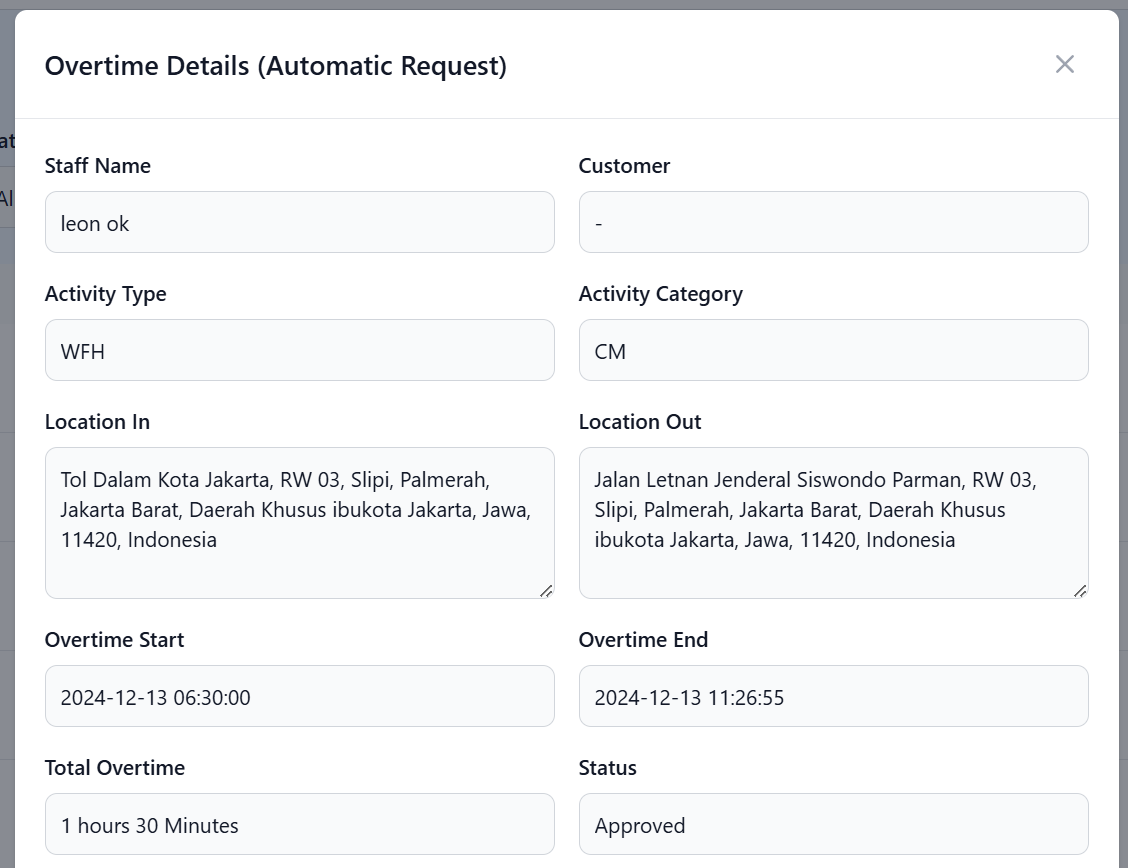
\includegraphics[width=9cm]{Gambar/bab4/pengujian-lembur-otomatis-overtime-4.png}
    	\caption{Hasil Riwayat Lembur Skenario Keempat}
    	\label{fig:hasil-riwayat-lembur-skenario-keempat}
        \end{figure}
        \FloatBarrier

Terakhir, skenario kelima akan dilakukan presensi masuk dan keluar saat \textit{shift}, namun pada hari tersebut terdapat hari libur perusahaan. Presensi masuk akan dilakukan pada hari Sabtu tanggal 14 Desember 2024 pukul 08.00 dan presensi keluar pada hari yang sama pukul 11.47. Hasil riwayat presensi pada skenario kelimat dapat dilihat pada \textbf{\ref{fig:hasil-riwayat-presensi-skenario-kelima}}.
\begin{figure}[!htbp]
    	\centering
    	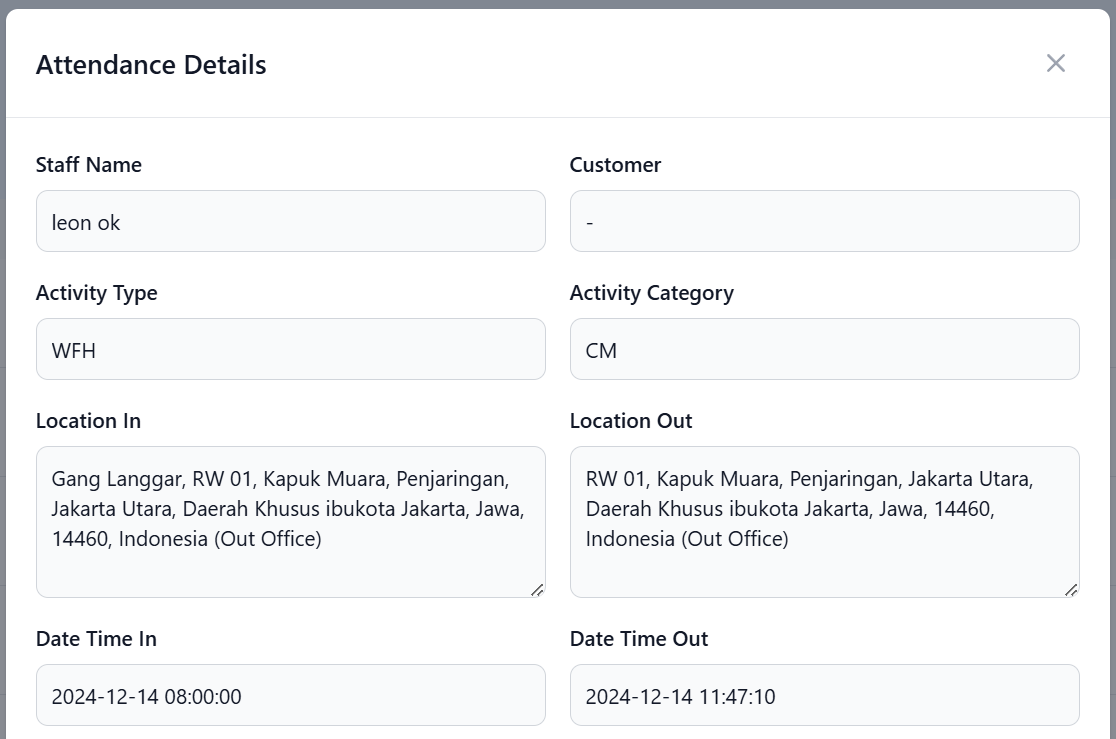
\includegraphics[width=9cm]{Gambar/bab4/pengujian-lembur-otomatis-attendance-5.png}
    	\caption{Hasil Riwayat Presensi Skenario Kelima}
    	\label{fig:hasil-riwayat-presensi-skenario-kelima}
        \end{figure}
        \FloatBarrier

Pada pengujian skenario kelima, sistem berhasil mendeteksi lembur walaupun pada hari tersebut terdapat \textit{shift} karena pada tanggal tersebut terdapat hari libur dari perusahaan. Sistem juga berhasil menghitung total jam lembur dengan sesuai yaitu 3 jam 47 menit. Hasil riwayat lembur skenario kelima dapat dilihat pada \textbf{\ref{fig:hasil-riwayat-lembur-skenario-kelima}}.
\begin{figure}[!htbp]
    	\centering
    	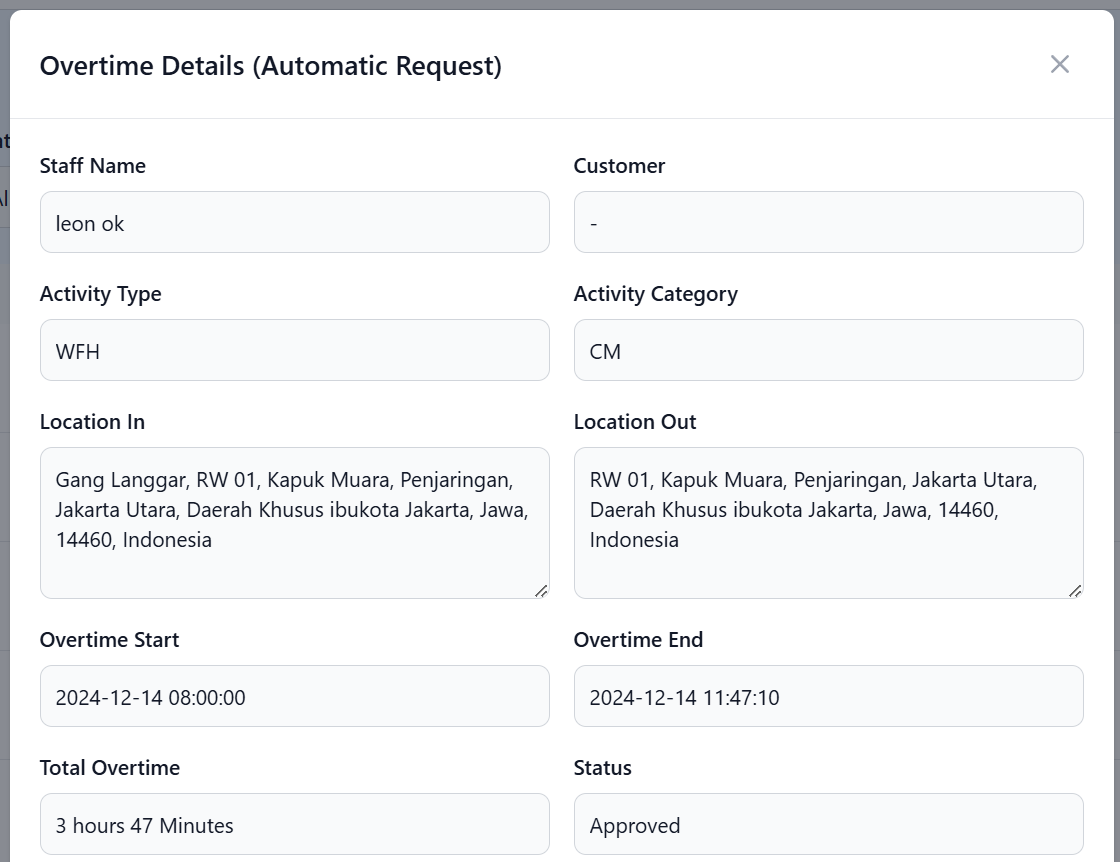
\includegraphics[width=9cm]{Gambar/bab4/pengujian-lembur-otomatis-overtime-5.png}
    	\caption{Hasil Riwayat Lembur Skenario Kelima}
    	\label{fig:hasil-riwayat-lembur-skenario-kelima}
        \end{figure}
        \FloatBarrier

Berdasarkan pengujian lembur otomatis dari 5 skenario yang berbeda, sistem berhasil mendeteksi adanya lembur jika presensi dilakukan diluar \textit{shift} yang telah ditentukan ataupun saat tanggal libur perusahaan. Sistem juga berhasil menghitung total jam lembur yang telah dilakukan dengan hasil yang akurat dan sesuai.

% \textbf{\ref{tab:table-skenario-perhitungan-lembur}} menunjukkan tabel hasil pengujian perhitungan lembur, seluruh tabel pengujian menunjukkan bahwa hasil yang diharapkan sesuai dengan hasil uji, sehingga dapat disimpulkan bahwa pengujian berhasil memenuhi semua kriteria yang telah ditetapkan.

% \begin{longtable}{ |p{1cm}|p{1.5cm}|p{1.5cm}|p{1.5cm}|p{3cm}|p{3cm}|}
% \caption{Tabel Skenario \textit{Test Case} Perhitungan Lembur}\label{tab:table-skenario-perhitungan-lembur} 
% \\
% \hline
% \textbf{Libur}
% &\textbf{Jadwal \textit{Shift}}
% &\textbf{Presensi Masuk}
% &\textbf{Presensi Keluar}
% &\textbf{Hasil Uji}
% &\textbf{Hasil Yang Diharapkan}
% \\ 
% \hline

% \multirow{1}{*}{Tidak}
% &Senin 08:00-17:00
% &Senin 06:00
% &Senin 08:00
% &Data lembur akan tercatat dengan total waktu 120 menit.
% &Data lembur berhasil tercatat dengan total waktu 120 menit.
% \\
% \hline

% \multirow{1}{*}{Tidak}
% &Senin 08:00-17:00
% &Senin 07:00
% &Senin 19:00
% &Data lembur akan tercatat dengan total waktu 180 menit.
% &Data lembur berhasil tercatat dengan total waktu 180 menit.
% \\
% \hline

% \multirow{1}{*}{Tidak}
% &Senin 08:00-17:00
% &Senin 17:00
% &Senin 18:15
% &Data lembur akan tercatat dengan total waktu 75 menit.
% &Data lembur berhasil tercatat dengan total waktu 75 menit.
% \\
% \hline

% \multirow{1}{*}{Tidak}
% &Senin 08:00-17:00
% &Senin 23:00
% &Selasa 01:00
% &Data lembur akan tercatat dengan total waktu 120 menit.
% &Data lembur berhasil tercatat dengan total waktu 120 menit.
% \\
% \hline

% \multirow{1}{*}{Ya}
% &Senin 08:00-17:00
% &Senin 08:00
% &Senin 12:00
% &Data lembur akan tercatat dengan total waktu 240 menit.
% &Data lembur berhasil tercatat dengan total waktu 240 menit.
% \\
% \hline


% \end{longtable}

\subsection{Pengujian TensorFlow}
Pada pengujian TensorFlow akan dilakukan dengan percobaaan pengambilan foto wajah melalui kamera perangkat pada saat presensi. Pada pengujian ini akan dilakukan beberapa skenario \textit{test case}. Pada skenaro pertama, akan dilakukan pengambilan foto saat presensi dengan tidak ada wajah pada kamera yang dapat dilihat pada \textbf{\ref{fig:pengambilan-foto-tidak-ada-wajah}}. Hasil yang diharapkan dari skenario ini adalah menampilkan pesan \textit{error} bahwa tidak ada wajah pada kamera. Hasil pengujian dapat dilihat pada \textbf{\ref{fig:hasil-uji-tidak-ada-wajah}}. Berdasarkan hasil pengujian dari skenario pertama didapatkan hasil yang sesuai dengan yang diharapkan.

Selanjutnya pada skenario kedua, akan dilakukan pengambilan foto wajah dengan posisi kepala diluar lingkaran putih pada kamera. \textbf{\ref{fig:pengambilan-foto-tidak-ditengah}} menunjukkan pengambilan foto wajah dengan posisi kepala diluar lingkaran putih. Hasil yang diharapkan dari skenario tersebut adalah menampilkan pesan \textit{error} bahwa pengambilan wajah, posisi kepala harus berada didalam lingkaran putih yang dapat dilihat pada \textbf{\ref{fig:hasil-uji-wajah-tidak-ditengah}}. Berdasarkan hasil pengujian didapatkan hasil yang sesuai dengan yang diharapkan.

\begin{figure}[!htbp]
    	\centering
    	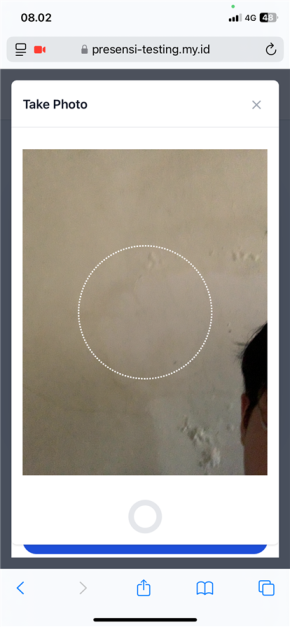
\includegraphics[width=4cm]{Gambar/bab4/pengambilan-foto-tidak-ada-wajah.PNG}
    	\caption{Tidak Ada Wajah Saat Pengambilan Foto}
    	\label{fig:pengambilan-foto-tidak-ada-wajah}
        \end{figure}
        \FloatBarrier

        \begin{figure}[!htbp]
    	\centering
    	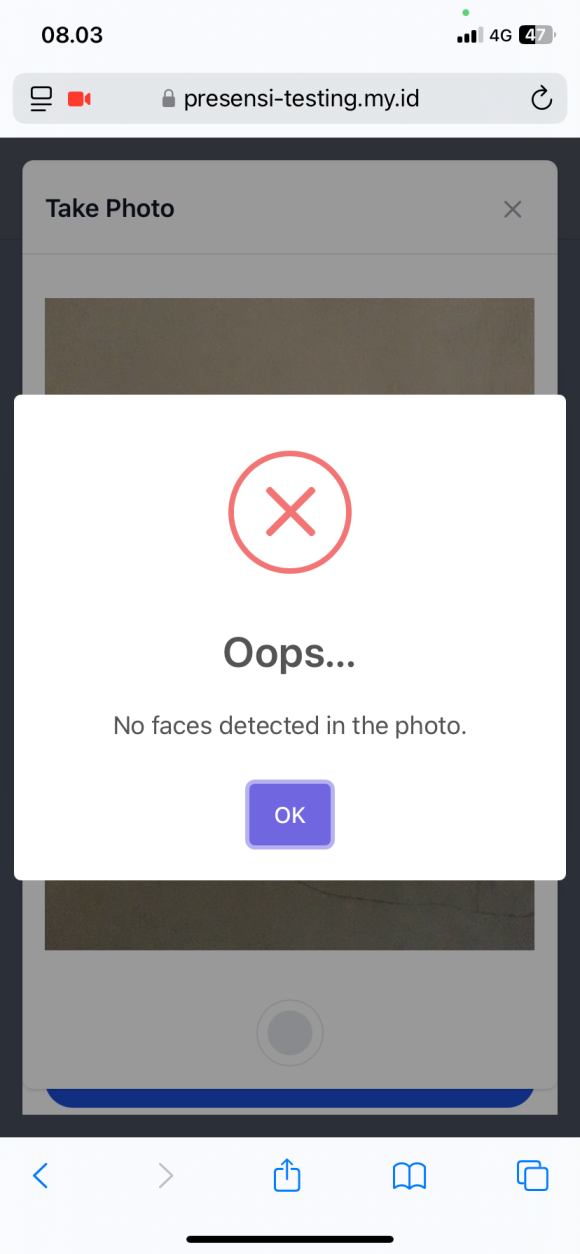
\includegraphics[width=4cm]{Gambar/bab4/hasil-uji-tidak-ada-wajah.PNG}
    	\caption{Hasil Uji Tidak Ada Wajah Saat Pengambilan Foto}
    	\label{fig:hasil-uji-tidak-ada-wajah}
        \end{figure}
        \FloatBarrier

\begin{figure}[!htbp]
    	\centering
    	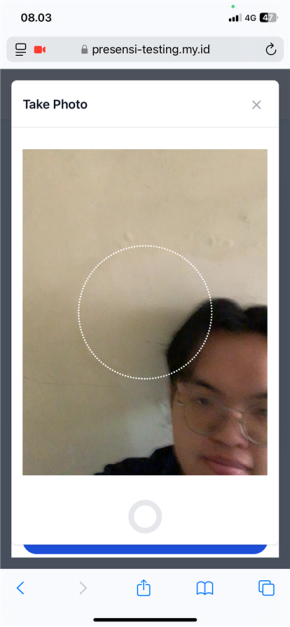
\includegraphics[width=4cm]{Gambar/bab4/pengambilan-foto-tidak-ditengah.PNG}
    	\caption{Posisi Wajah Tidak Ditengah Saat Pengambilan Foto}
    	\label{fig:pengambilan-foto-tidak-ditengah}
        \end{figure}
        \FloatBarrier

        \begin{figure}[!htbp]
    	\centering
    	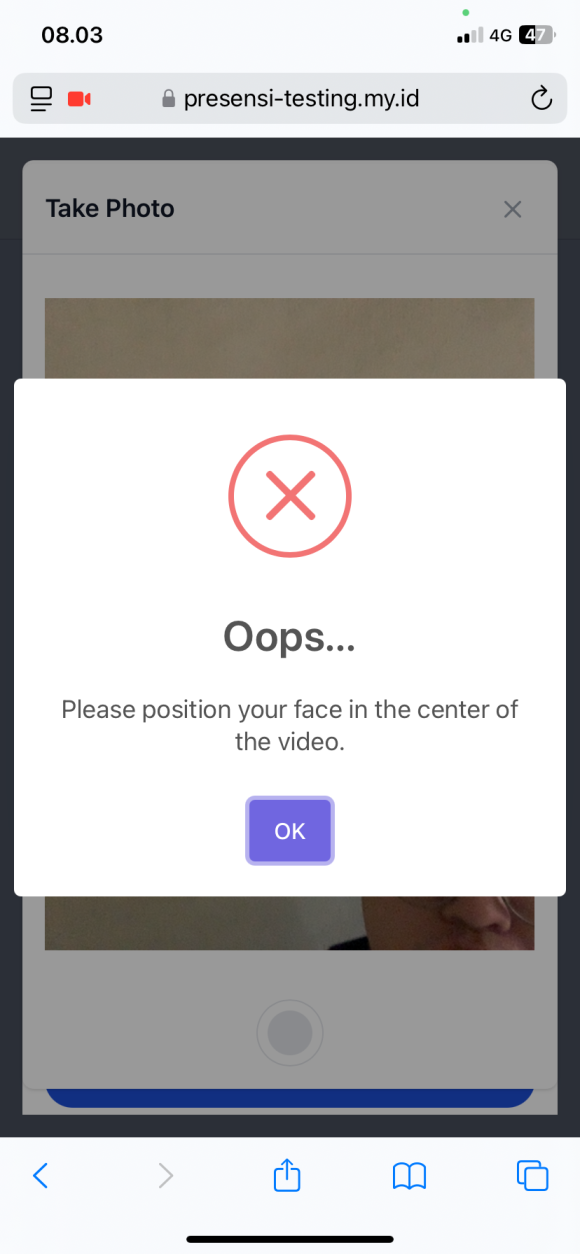
\includegraphics[width=4cm]{Gambar/bab4/hasil-uji-wajah-tidak-ditengah.PNG}
    	\caption{Hasil Uji Posisi Wajah Tidak Ditengah Saat Pengambilan Foto}
    	\label{fig:hasil-uji-wajah-tidak-ditengah}
        \end{figure}
        \FloatBarrier

Setelah itu, pada skenario ketiga dilakukan pengambilan foto wajah didalam lingkaran putih, namun posisi kepala terlalu dekat dengan kamera sehingga posisi kepala keluar dari batas lingkaran putih yang dapat dilihat pada \textbf{\ref{fig:pengambilan-foto-terlalu-dekat}}. Hasil yang diharapkan dari skenario ini yaitu menampilkan pesan \textit{error} bahwa wajah terlalu dekat dengan kamera. \textbf{\ref{fig:hasil-uji-wajah-terlalu-dekat}} menunjukkan hasil yang didapat dari pengujian. Berdasarkan hasil pengujian didapatkan hasil yang sesuai dengan yang diharapkan.

\begin{figure}[!htbp]
    	\centering
    	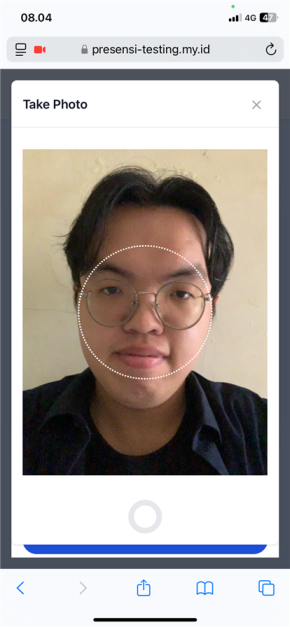
\includegraphics[width=4cm]{Gambar/bab4/pengambilan-foto-terlalu-dekat.PNG}
    	\caption{Posisi Wajah Dekat Dengan Kamera Saat Pengambilan Foto}
    	\label{fig:pengambilan-foto-terlalu-dekat}
        \end{figure}
        \FloatBarrier

        \begin{figure}[!htbp]
    	\centering
    	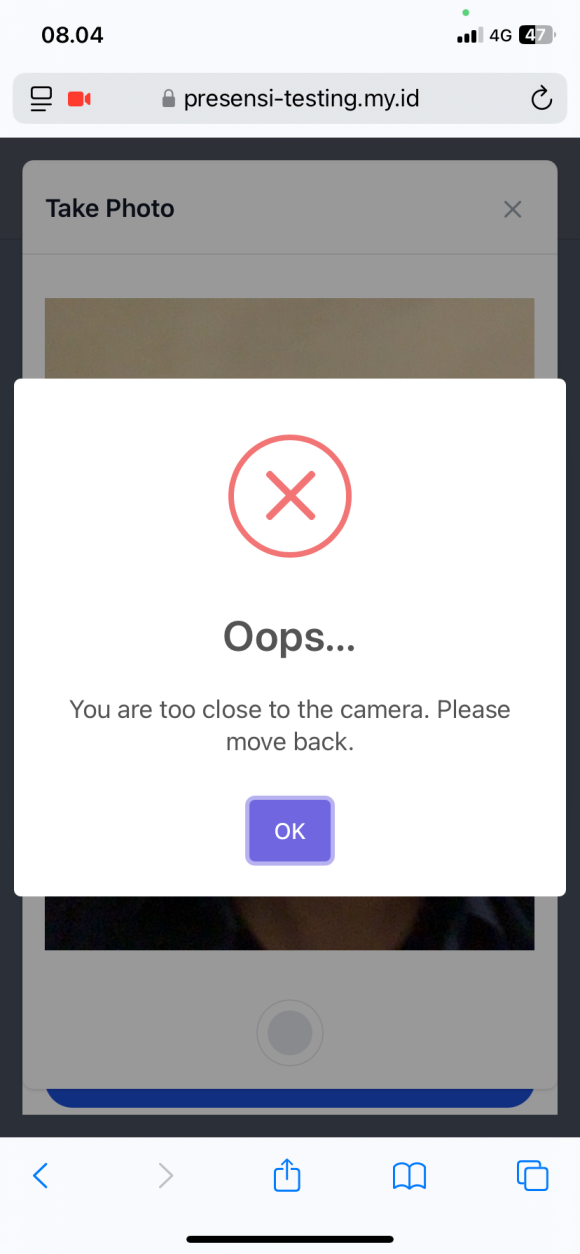
\includegraphics[width=4cm]{Gambar/bab4/hasil-uji-wajah-terlalu-dekat.PNG}
    	\caption{Hasil Uji Posisi Wajah Dekat Dengan Kamera Saat Pengambilan Foto}
    	\label{fig:hasil-uji-wajah-terlalu-dekat}
        \end{figure}
        \FloatBarrier

Terakhir, pada skenario keempat dilakukan pengambilan foto wajah yang tepat posisinya didalam lingkaran putih yang dapat dilihat pada \textbf{\ref{fig:pengambilan-foto-pas}}. Hasil yang diharapkan dari pengujian ini adalah modal Kamera akan tertutup dan menampilkan hasil \textit{preview} foto pada modal presensi. Hasil pengujian dapat dilihat pada \textbf{\ref{fig:hasil-uji-foto-pas}}. Berdasarkan hasil pengujian didapatkan hasil yang sesuai dengan yang diharapkan. Seluruh skenario pengujian memberikan hasil yang sesuai sehingga fitur validasi wajah pada aplikasi presensi \textit{online} berfungsi dengan baik.

\begin{figure}[!htbp]
    	\centering
    	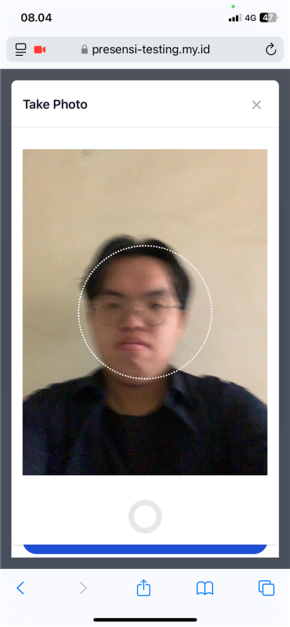
\includegraphics[width=4cm]{Gambar/bab4/pengambilan-foto-pas.PNG}
    	\caption{Posisi Wajah Tepat Didalam Lingkaran Saat Pengambilan Foto}
    	\label{fig:pengambilan-foto-pas}
        \end{figure}
        \FloatBarrier

        \begin{figure}[!htbp]
    	\centering
    	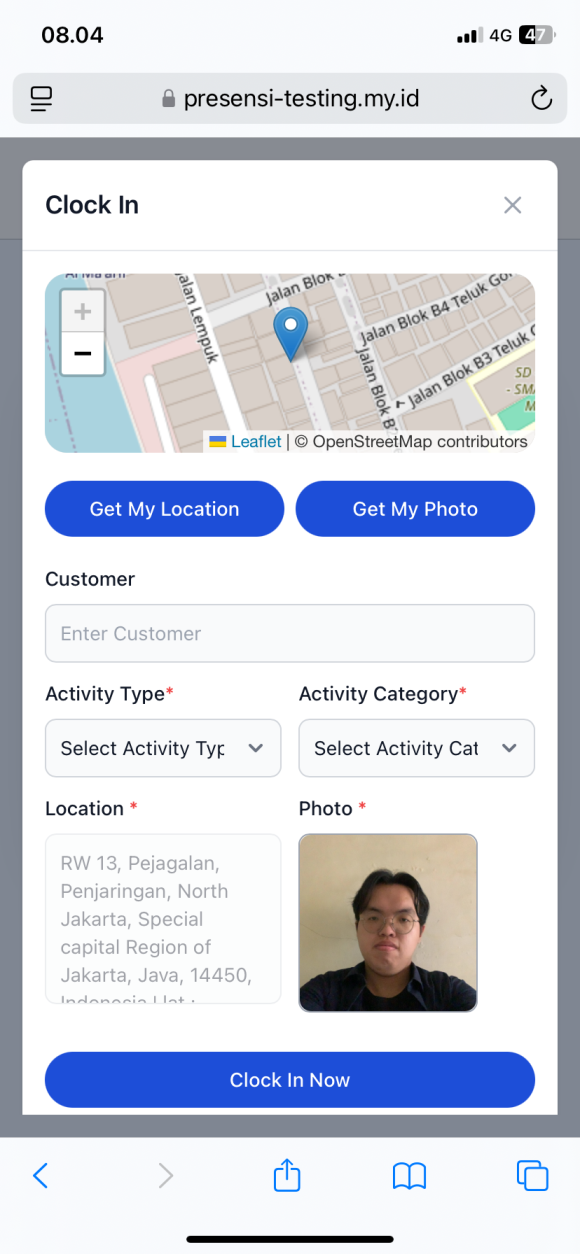
\includegraphics[width=4cm]{Gambar/bab4/hasil-uji-foto-pas.PNG}
    	\caption{Hasil Uji Posisi Wajah Tepat Didalam Lingkaran Saat Pengambilan Foto}
    	\label{fig:hasil-uji-foto-pas}
        \end{figure}
        \FloatBarrier

\subsection{Pengujian oleh Pengguna \textit{Non}-IT}
Pengujian oleh user \textit{non}-IT akan dilakukan menggunakan metode \textit{blackbox testing}, seperti yang telah dilakukan sebelumnya, serta metode SUS (\textit{System Usability Scale}) kepada \textit{staff} MyPassword yang bekerja di divisi \textit{non}-IT seperti \textit{sales, driver, product specialist, business support, digital marketing,} dan \textit{admin}. Pengujian dilakukan pada tanggal 12 hingga 13 Desember 2024 secara luring di MyPassword. Hasil pengujian \textit{blackbox testing} kepada \textit{staff} MyPassword divisi \textit{non-}IT dapat dilihat pada \textbf{\hyperref[sec:blackbox-testing-aplikasi-presensi-online-oleh-pengguna-non-it]{Lampiran~XIX}}.

Selanjutnya dilakukan juga SUS (\textit{System Usability Scale}) kepada \textit{staff} MyPassword divisi \textit{non-}IT. Menurut Albert dan Tullis~\cite{measuring2022bill}, SUS (\textit{System Usability Scale}) merupakan salah satu alat yang paling banyak digunakan untuk menilai persepsi kegunaan suatu sistem atau produk. SUS terdiri dari 10 pernyataan yang dinilai oleh pengguna berdasarkan tingkat kesetujuan pengguna. Setengah dari pernyataan tersebut menggunakan kata-kata positif, sementara setengah lainnya menggunakan kata-kata negatif. Skala kesetujuan 5 poin digunakan untuk setiap pernyataan yang terdiri dari pilihan sangat setuju, setuju, ragu-ragu, tidak setuju, dan sangat tidak setuju. Berikut ini adalah 10 pertanyaan pada pengujian SUS:
\begin{enumerate}
    \item Saya berpikir bahwa saya akan sering menggunakan sistem ini.
    \item Saya merasa sistem ini terlalu rumit tanpa alasan.
    \item Saya merasa sistem ini mudah digunakan.
    \item Saya berpikir bahwa saya akan membutuhkan bantuan teknisi untuk dapat menggunakan sistem ini.
    \item Saya merasa berbagai fungsi dalam sistem ini terintegrasi dengan baik.
    \item Saya merasa ada terlalu banyak inkonsistensi dalam sistem ini.
    \item Saya membayangkan bahwa kebanyakan orang akan cepat belajar menggunakan sistem ini.
    \item Saya merasa sistem ini sangat merepotkan untuk digunakan.
    \item Saya merasa sangat percaya diri menggunakan sistem ini.
    \item Saya perlu mempelajari banyak hal sebelum bisa mulai menggunakan sistem ini.
\end{enumerate}

Cara untuk menghitung skor SUS yaitu dengan menjumlahkan kontribusi skor dari setiap pertanyaan, di mana setiap kontribusi skor bernilai antara 0 hingga 4. Untuk pertanyaan bernomor ganjil (1, 3, 5, 7, dan 9), kontribusi skor dihitung dengan mengurangi 1 dari posisi pada skala. Sedangkan untuk pertanyaan bernomor genap (2, 4, 6, 8, dan 10), kontribusinya dihitung dengan mengurangi posisi pada skala dari 5. Setelah semua kontribusi dijumlahkan, kalikan hasilnya dengan 2,5 untuk memperoleh skor SUS secara keseluruhan. Hasil dari perhitungan skor SUS digunakan untuk menentukan peringkat. \textbf{\ref{fig:tabel-peringkat-sus}} menunjukkan peringkat berdasarkan skor SUS.
\begin{figure}[!htbp]
    	\centering
    	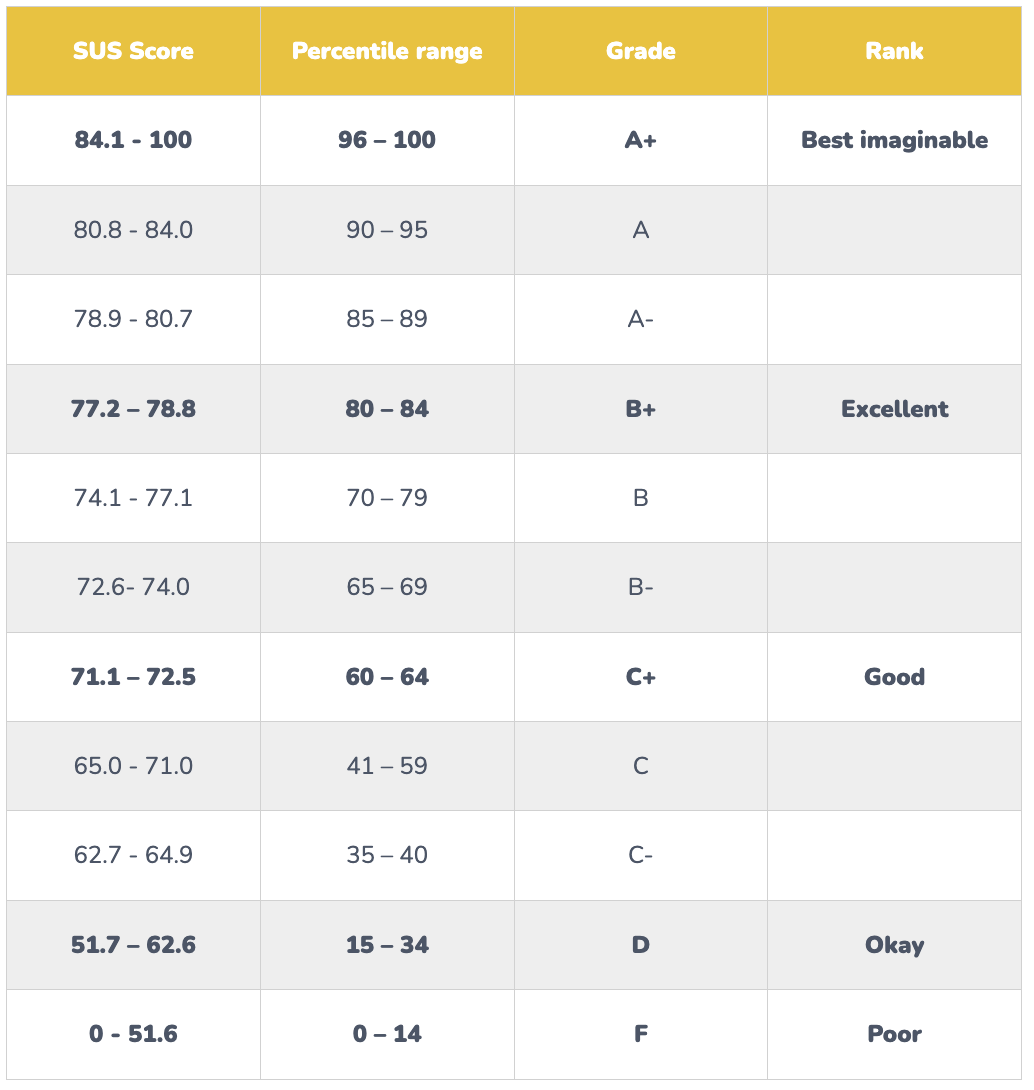
\includegraphics[width=10cm]{Gambar/bab4/tabel-peringkat-sus.png}
    	\caption{Peringkat SUS\cite{system2024john}}
    	\label{fig:tabel-peringkat-sus}
        \end{figure}
        \FloatBarrier

\begin{figure}[!htbp]
    	\centering
    	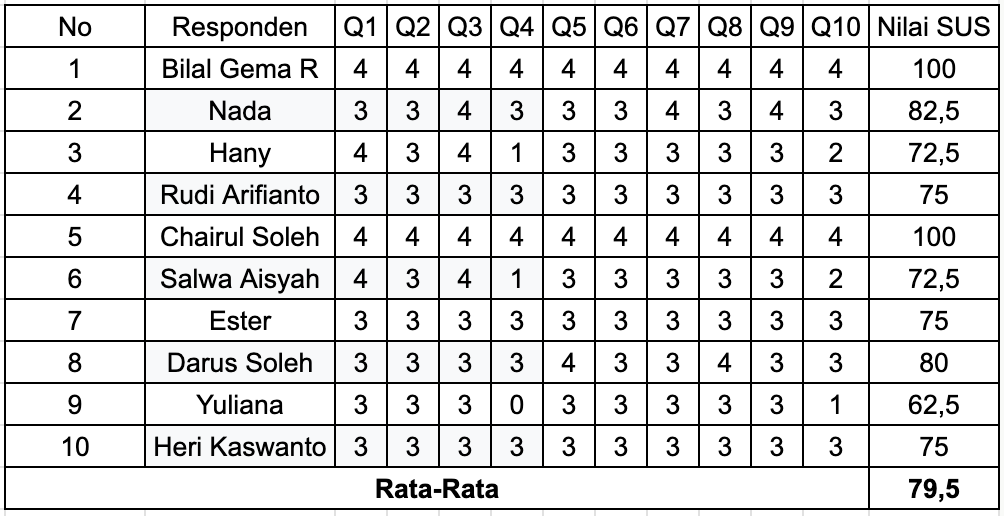
\includegraphics[width=13cm]{Gambar/bab4/hasil-sus.png}
    	\caption{Hasil Pengujian SUS}
    	\label{fig:hasil-pengujian-sus}
        \end{figure}
        \FloatBarrier
        
Pengujian SUS pada aplikasi presensi \textit{online} berbasis web menggunakan \textit{Google Form} melalui tautan \url{https://forms.gle/WrkckqFsDjx8AryZ6}. Pada pengujian ini didapatkan 10 responden yang memiliki rentang umur antara 24-53 tahun dengan latar belakang pekerjaan \textit{non}-IT. Hasil pengujian SUS dengan \textit{staff} MyPassword \textit{non-}IT dapat dilihat pada \textbf{\ref{fig:hasil-pengujian-sus}}. Grafik hasil pengujian dan perhitungan skor SUS dapat dilihat pada \textbf{\ref{fig:grafik-pengujian-sus}}. Berdasarkan rata-rata hasil pengujian SUS dari 10 responden, diperoleh skor SUS sebesar 79,5, yang termasuk dalam peringkat A- pada skala SUS.
\begin{figure}[!htbp]
    	\centering
    	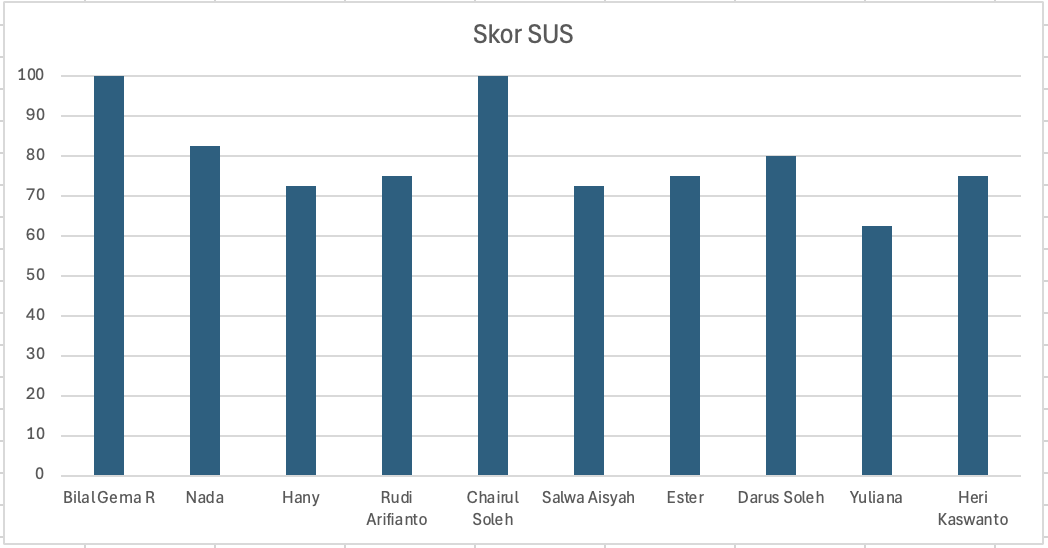
\includegraphics[width=13cm]{Gambar/bab4/grafik-sus.png}
    	\caption{Grafik Pengujian SUS}
    	\label{fig:grafik-pengujian-sus}
        \end{figure}
        \FloatBarrier

Dokumentasi pengujian \textit{blackbox testing} dan pengujian SUS bersama \textit{staff} MyPassword dengan latar belakang pekerjaan \textit{non-}IT dapat dilihat pada \textbf{\hyperref[sec:dokumentasi-blackbox-testing-dan-sus-bersama-staff-non-it]{Lampiran~XX}}.
\chapter{KESIMPULAN DAN SARAN}

\section{Kesimpulan}
Kesimpulan dari perancangan aplikasi presensi \textit{online} berbasis web pada PT Password Solusi Sistem yaitu sebagai berikut:
\begin{enumerate}
    \item Aplikasi presensi \textit{online} berhasil mengimplementasikan teknik \textit{Geolocation} untuk memperoleh lokasi pengguna dengan tingkat akurasi yang baik. Selain itu, algoritma Haversine diterapkan untuk menghitung jarak antara lokasi \textit{Staff Infrastructure} dengan lokasi kantor MyPassword. Pengujian akurasi perhitungan dilakukan dengan membandingkan hasil algoritma Haversine dengan \textit{Google Geometry} API, menghasilkan rata-rata selisih sebesar 0,0113 km dari 20 lokasi yang berbeda.
    \item Aplikasi presensi \textit{online} mendukung manajer dalam proses perhitungan lembur melalui fitur perhitungan lembur otomatis. Fitur ini berfungsi ketika \textit{Staff Infrastructure} melakukan presensi di luar jadwal \textit{shift} atau pada hari libur perusahaan. Pengujian fitur ini dilakukan melalui beberapa skenario pengujian (\textit{test case}), yang menunjukkan hasil perhitungan yang akurat dan sesuai dengan kebutuhan.
    \item Aplikasi presensi \textit{online} dilengkapi dengan fitur validasi wajah berbasis TensorFlow, yang mengharuskan wajah \textit{Staff Infrastructure} terdeteksi sebelum presensi dapat dilakukan. Pengujian fitur validasi wajah dilakukan menggunakan berbagai skenario pengujian, yang seluruhnya menunjukkan hasil yang sesuai dengan harapan.
    \item Aplikasi presensi \textit{online} berbasis web telah dilakukan pengujian kepada 10 \textit{staff non-}IT MyPassword dengan metode \textit{blackbox testing} yang mendapatkan hasil valid untuk semua skenario dan pengujian SUS juga dilakukan yang mendapatkan hasil skor 79,5 yang merupakan peringkat A-.
    
\end{enumerate}


\section{Saran}
Berikut ini adalah beberapa saran untuk pengembangan lebih lanjut dari aplikasi presensi \textit{online} berbasis web:
\begin{enumerate}
    \item Saat ini aplikasi sudah memiliki fitur deteksi wajah saat pengambilan foto presensi, namun akan lebih baik jika dilengkapi dengan verifikasi wajah pengguna untuk memastikan kesesuaian dengan foto yang terdaftar sebelumnya seperti integrasi dengan \textit{library FaceApi JS}.
    \item Meningkatkan tampilan \textit{User Interface} (UI) yang lebih baik.
    \item Menambah fitur untuk perhitungan gaji serta mengintegrasikan fitur penggajian kepada karyawan secara otomatis.
\end{enumerate}


\bibliographystyle{IEEEtranN}
% \bibliographystyle{unsrtnat}  % Choose your desired bibliography style

%  \renewcommand{\thefigure}{2.\arabic{figure}}

% \renewcommand{\thetable}{2.\arabic{table}}

% \bibliographystyle{unsrt}
\bibliography{references}
\addcontentsline{toc}{chapter}{DAFTAR PUSTAKA}
\begin{landscape}
    
\chapter*{\centering LAMPIRAN}
\addcontentsline{toc}{chapter}{LAMPIRAN}
\newcommand\Plabel[1]{\makebox[1in][l]{#1}}

\nextappendix
\section*{Lampiran \theappendixletter: Referensi \label{sec:referensi}}
\addcontentsline{toc}{section}{Lampiran \theappendixletter: Referensi}
\begin{longtable}{ |p{0.5cm}|p{3cm}|p{7cm}|p{12cm}|  }
	\caption{Tabel Referensi}\label{tab:referensi} \\
	\hline
	\multicolumn{1}{|c|}{\textbf{No}} & \multicolumn{1}{|c|}{\textbf{Sumber}} & \multicolumn{1}{|c|}{\textbf{Hasil Aplikasi}} & \multicolumn{1}{|c|}{\textbf{Perbedaan}} \\ \hline
	1 
 & Pengembangan Sistem Informasi Presensi Menggunakan Metode Waterfall.
 \newline Tri Wahyudi, Supriyanta Supriyanta, Husni Faqih.
 \newline Indonesian Journal On Software Engineering (IJSE)
 \newline ISSN : 2714-9935 
 & Sistem Informasi Presensi yang dikembangkan dengan metode pengembangan software Waterfall menghasilkan aplikasi yang berfungsi untuk menyediakan solusi terhadap masalah presensi karyawan dan siswa selama pandemi Covid-19. Aplikasi ini terdapat 2 pengguna yaitu karyawan dan admin. Karyawan dapat melakukan presensi serta melihat \textit{history} presensi, sedangkan admin dapat mengelola data karyawan, jam kerja karyawan, mengelola data presensi, dan mencetak rekap presensi. 
 & Pada jurnal sistem informasi presensi yang dikembangkan dengan metode pengembangan software waterfall, terdapat 2 \textit{role user} yaitu karyawan dan admin. Karyawan dapat melakukan presensi secara \textit{online} tapi data lokasi dan foto tidak dicatat, serta tidak terdapat sistem untuk melakukan perhitungan jam lembur.
 \newline 
  \newline
  Sedangkan pada aplikasi presensi \textit{online} berbasis \textit{web} pada PT Password Solusi Sistem menggunakan metode \textit{scrum}. Aplikasi ini terdapat 3 \textit{role user} yaitu \textit{manager} HRD, \textit{manager Infrastructure}, dan \textit{staff}. \textit{Staff} dapat melakukan presensi secara \textit{online} dan data lokasi serta foto akan dicatat oleh sistem. Selain itu, sistem akan melakukan perhitungan lembur jika \textit{staff} melakukan presensi diluar jam kerja atau pada hari libur.
 \\ \hline
 
 2 & APLIKASI PRESENSI ONLINE MENGGUNAKAN VALIDASI JARAK LOKASI PENGGUNA BERBASIS ANDROID (STUDY KASUS: TOKO YONIX)
 \newline Bayu Adytia Permana, Kisworo, Akhmad Jayadi.
 \newline Jurnal Informatika dan Rekayasa Perangkat Lunak (JATIKA)
 \newline ISSN : 2797-2011 
 & Aplikasi presensi \textit{online} menggunakan validasi jarak lokasi pengguna berbasis Android (study kasus: toko Yonix) berhasil dibangun berdasarkan model pada jurnal ini dan validasi jarak berhasil diterapkan menggunakan perhitungan antar lokasi yaitu pengguna dan toko, kemudian karyawan berhasil melakukan absensi secara tepat dan sesuai harapan. Terdapat 2 \textit{role} pada aplikasi ini. \textit{Role} karyawan dapat \textit{login}, melihat lokasi antara pengguna dan toko, absen kehadiran, dan informasi presensi karyawan. Sedangkan \textit{role} admin dapat login, melihat absen harian, dan melihat absen berdasarkan tanggal.
 & Pada jurnal aplikasi presensi \textit{online} menggunakan validasi jarak lokasi pengguna berbasis Android (study kasus: toko Yonix) dikembangkan berbasis android dan terdapat 2 \textit{role} yaitu karyawan dan admin. Karyawan hanya bisa \textit{login} dan melakukan presensi \textit{online} dan saat presensi juga menggunakan fitur GPS tapi hanya untuk melihat jarak antara pengguna dan toko saja dan tidak ada pengambilan foto. Selanjutnya pada \textit{role} admin dapat login, menambah data karyawan, dan mencari data absensi karyawan.
 \newline 
  \newline
  Sedangkan pada aplikasi presensi \textit{online} berbasis \textit{web} pada PT Password Solusi Sistem dikembangakan berbasis \textit{web} dan terdapat 3 \textit{role}. \textit{Role staff} dapat \textit{register/login}, melihat jadwal kerja, melakukan absensi dengan fitur GPS untuk mencatat lokasi pengguna dan mengambil foto pengguna serta sistem akan mencatat dan menghitung jam kerja lembur jika presensi dilakukan diluar jam kerja. Selanjutnya \textit{role manager} Infra yaitu dapat \textit{register/login}, dapat melakukan \textit{reject} pada data lembur yang tidak valid serta melihat data lembur \textit{staff}. Setelah itu, \textit{role manager} HRD dapat melakukan pengaktifan akun jika pengguna sudah \textit{register}, melihat data presensi dan lembur, serta mengelola data hari libur nasional dan jam kerja karyawan yang digunakan untuk mendeteksi jam lembur saat presensi.
 \\ \hline

  3 & Sistem Informasi Presensi Karyawan Berbasis Android (Studi Kasus: Asuransi Panin Dai-Ichi Life)
 \newline Tasya Rizki Ramadhini, Fenty Ariany, Akhmad Jayadi
 \newline Jurnal Teknologi dan Sistem Informasi (JTSI)
 \newline ISSN : 2746-3699
 & Sistem Informasi Presensi Karyawan Berbasis Android (Studi Kasus: Asuransi Panin Dai-Ichi Life) menggunakan implementasi GPS dengan metode geofence untuk mencari posisi devide saat karyawan melakukan presensi dan menggunakan metode Haversine Formula yang digunakan untuk mengetahui jarak radius lokasi agar dapat melakukan presensi. Pada aplikasi ini dirancang untuk pegawai saja yang dapat melakukan presensi dalam radius kantor dan pengambilan foto, terdapat menu form yang dapat digunakan oleh pegawai untuk izin atau sakit, terdapat menu untuk melihat history presensi, dan menu untuk melihat jadwal kerja.
 & Pada jurnal Sistem Informasi Presensi Karyawan Berbasis Android (Studi Kasus: Asuransi Panin Dai-Ichi Life) dikembangkan berbasis Android dan menggunakan metode \textit{waterfall}. Pada aplikasi ini menggunakan GPS hanya untuk membatasi radius saat melakukan presensi. Aplikasi ini hanya dirancang untuk \textit{role} pegawai saja yang dapat melakukan presensi, pengajuan izin atau sakit, melihat jadwal kerja, dan riwayat presensi.
 \newline 
  \newline
  Sedangkan pada aplikasi presensi \textit{online} berbasis \textit{web} pada PT Password Solusi Sistem dikembangkan berbasis \textit{web} dan menggunakan metode \textit{scrum}. Aplikasi ini menggunakan GPS untuk pencatatan lokasi saat presensi dan dikembangkan untuk 3 \textit{role} yaitu \textit{staff Infrastructure}, \textit{manager Infrastructure}, dan \textit{manager} HRD. Aplikasi ini juga dilengkapi sistem untuk melakukan pencatatan dan perhitungan lembur jika \textit{staff} melakukan presensi diluar jam kerja dan terdapat \textit{form} pengajuan lembur jika \textit{staff} lupa presensi saat lembur, akan tetapi aplikasi ini tidak ada \textit{form} untuk pengajuan izin atau sakit.
 \\ \hline

  4 & RANCANG BANGUN APLIKASI SISTEM INFORMASI ABSENSI KARYAWAN ONLINE
 \newline Rully Roosdianto, Ani Oktarini Sari, Arief Satriansyah
 \newline Jurnal Inti Nusa Mandiri
 \newline ISSN : 2685-807X
 & Rancang bangun aplikasi sistem informasi absensi karyawan online menghasilkan aplikasi yang dapat mempermudah karyawan dalam proses absensi, melakukan pencarian data absensi, menghitung seluruh rekap absensi karyawan, serta mengurangi resiko kehilangan dan kesalahan dalam pencatatan absensi pada CV Cahaya Toner. Aplikasi ini berbasis \textit{web} yang terdiri dari 2 \textit{role} yaitu \textit{admin} dan karyawan. \textit{Admin} dapat mengelola data karyawan, melihat rekap absensi, mengelola divisi, dan mengelola jam kerja karyawan. Sedangkan pada \textit{role} karyawan hanya dapat melakukan absensi dan melihat riwayat absensi.
 & Pada jurnal Rancang Bangun Aplikasi Sistem Informasi Absensi Karyawan Online dirancang berbasis \textit{web} menggunakan \textit{framework Codeigniter} dan menggunakan metode \textit{waterfall}. aplikasi ini hanya terdiri dari 2 \textit{role} yaitu \textit{admin} dan karyawan. Karyawan dapat melakukan absensi secara \textit{online} tapi saat proses tersebut tidak dilakukan pencatatan lokasi dan pengambilan foto.
 \newline 
  \newline
  Sedangkan pada aplikasi presensi \textit{online} berbasis \textit{web} pada PT Password Solusi Sistem dikembangkan berbasis \textit{web} dengan \textit{framwork Laravel} dan menggunakan metode \textit{scrum}. Aplikasi ini terdiri dari 3 \textit{role} yaitu \textit{staff Infrastructure}, \textit{manager Infrastructure}, dan \textit{manager} HRD. \textit{Staff Infrastructure} dapat melakukan presensi secara \textit{online} dengan tambahan teknik \textit{geolocation} yang dapat digunakan untuk mendapat titik koordinat \textit{staff} dan mencatat lokasi tersebut, aplikasi ini juga melakukan pengambilan foto saat presensi serta dilengkapi sistem untuk mendeteksi dan menghitung jam lembur jika \textit{staff} melakukan presensi diluar jam kerja. Data lembur yang masuk memiliki fitur \textit{reject} dari \textit{manager Infrastructure} atau penolakkan jika data lembur tidak \textit{valid}.
 \\ \hline

 
   5 & PENGEMBANGAN SISTEM ABSENSI ONLINE BERBASIS WEB MENGGUNAKAN MAPS JAVASRIPTS API
 \newline Gerlan Apriandy Manu, Yonly Adrianus Benufinit
 \newline Jurnal Pendidikan Teknologi Informasi (JUKANTI)
 \newline ISSN : 2621-1467
 & Pengembangan sistem absensi \textit{online} berbasis \textit{web} menggunakan \textit{maps javascripts API} menghasilkan aplikasi absensi \textit{online} yang dapat menyimpan \textit{latitude} dan \textit{longitude} pada \textit{user} yang melakukan absensi \textit{online} sehingga aplikasi ini dapat membantu manajemen absensi karyawan saat WFH (\textit{Work From Home}), yaitu melakukan absensi dimana pun dan kapanpun tanpa harus datang ke kantor menggunakan absensi \textit{fingerprint}. Aplikasi ini terdiri dari 2 \textit{role} yaitu pegawai dan petugas absensi. Pegawai dapat melakukan absensi secara \textit{online}, aplikasi ini menggunakan \textit{javascripts API} untuk mendapatkan lokasi dan mencatatnya, aplikasi juga mengambil foto selfie pegawai saat absensi, serta melihat riwayat absensi. Selanjutnya \textit{role} petugas absensi dapat melihat rekap absensi karyawan setiap bulan pada tanggal 20.
 & Pada jurnal Pengembangan sistem absensi \textit{online} berbasis \textit{web} menggunakan \textit{maps javascripts API} dikembangkan dengan \textit{PHPMaker} dan metode RAD (\textit{Rapid Application Development}). Aplikasi ini terdiri dari 2 \textit{role} yaitu pegawai dan petugas absensi. Aplikasi ini menggunakan API untuk mengambil dan mencatat lokasi karyawan dan foto pegawai saat presensi, namun tidak terdapat fitur jadwal kerja karyawan dan tidak bisa mendeteksi dan menghitung jumlah jam lembur pegawai jika presensi dilakukan pada hari libur atau diluar jam kerja.
 \newline 
  \newline
  Sedangkan pada aplikasi presensi \textit{online} berbasis \textit{web} pada PT Password Solusi Sistem dikembangkan berbasis \textit{web} dengan \textit{framwork Laravel} dan menggunakan metode \textit{scrum}. Aplikasi ini terdiri dari 3 \textit{role} yaitu \textit{staff Infrastructure}, \textit{manager Infrastructure}, dan \textit{manager} HRD. Aplikasi ini juga menggunakan bantuan API untuk mendapat lokasi \textit{staff} saat presensi namun dengan tambahan sistem untuk menghitung dan mencatat jam lembur \textit{staff} jika presensi dilakukan diluar \textit{shift} yang ditentukan. Data lembur yang masuk dapaat di-\textit{reject} oleh \textit{Manager Infrastructure} jika data lembur tersebut tidak \textit{valid}.
 \\ \hline

  6 & Perancangan Aplikasi Absensi Online Dengan Menggunakan Bahasa Pemrograman Kotlin
 \newline Arafat Febriandirza
 \newline Jurnal Pseudocode
 \newline ISSN : 2655-1845
 & Perancangan aplikasi absensi online dengan menggunakan bahasa pemrograman kotlin menghasilkan sistem yang membuat karyawan menjadi lebih disiplin, mengurangi kemungkinan adanya kecurangan saat melakukan absensi, meningkatkan efisiensi dan akurasi pencatatan data dan mengetahui lokasi karyawan saat absensi. Aplikasi ini memiliki 2 \textit{role} yaitu karyawan dan HRD karyawan. Karyawan dapat melakukan absensi \textit{online}, melihat data absensi, melakukan penugasan dan melihat data penugasan. Aplikasi ini dilengkapi GPS untuk mendapatkan alamat lokasi saat absensi.
 & Pada jurnal Perancangan aplikasi absensi online dengan menggunakan bahasa pemrograman kotlin dirancang berbasis Android dengan bahasa pemrograman \textit{kotlin} dan menggunakan metode \textit{agile}. Aplikasi ini dibagi menjadi 2 \textit{role} yaitu karyawan dan HRD Karyawan. Aplikasi ini sama-sama menggunakan GPS untuk mendapatkan lokasi \textit{user} namun aplikasi ini tidak terdapat pengambilan foto saat absensi dan tidak ada jadwal \textit{shift} karyawan dan sistem untuk mencatat dan menghitung jam lembur jika karyawan melakukan absensi diluar jam kerja atau pada hari libur.
 \newline 
  \newline
  Sedangkan pada aplikasi presensi \textit{online} berbasis \textit{web} pada PT Password Solusi Sistem dikembangkan berbasis \textit{web} dengan \textit{framwork Laravel} dan menggunakan metode \textit{scrum}. Aplikasi ini terdiri dari 3 \textit{role} yaitu \textit{staff Infrastructure}, \textit{manager Infrastructure}, dan \textit{manager} HRD. Aplikasi ini dilengkapi pengambilan foto \textit{user} saat melakukan presensi dan fitur tambahan untuk mendeteksi jam lembur berdasarkan \textit{shift} kerja \textit{staff}, jika \textit{staff} melakukan presensi diluar jam kerja maka akan masuk ke dalam data lembur. Data lembur dapat di-\textit{reject} oleh \textit{Manager Infrastructure} jika data lembur tersebut tidak \textit{valid}.
 \\ \hline

   7 & PERANCANGAN SISTEM INFORMASI ABSENSI ONLINE DETEKSI LOKASI BERBASIS WEB
 \newline Bryan Daniel Pesik, Penidas Fiodinggo Tanaem
 \newline Jurnal Mahasiswa Teknik Informatika (JATI)
 \newline ISSN : 2598-828X
 & Perancangan sistem informasi absensi \textit{online} deteksi lokasi berbasis \textit{web} menghasilkan aplikasi yang mempermudah kantor BPKAD untuk melakukan absensi dan merekap data laporan absensi karena data yang tersimpan didalam database. Aplikasi ini memiliki 2 \textit{role} yaitu pegawai dan \textit{admin}. Pegawai dapat melakukan absen pulang dan absen datang. Kemudian pada \textit{role admin} dapat merekap data absensi, mengatur jam kerja, melihat lokasi absen dan melihat data pegawai.
 & Pada jurnal Perancangan sistem informasi absensi \textit{online} deteksi lokasi berbasis \textit{web} dikembangkan dengan PHP dan \textit{framework Bootstrap}. Aplikasi ini memiliki 2 \textit{role} yaitu pegawai dan \textit{admin}. Pegawai dapat melakukan absensi tanpa fitur tambahan perhitungan lembur jika absensi dilakukan diluar jam kerja atau hari libur. Pada \textit{role admin} dapat mengatur jam kerja tapi untuk seluruh pegawai jadi kurang fleksibel.
 \newline 
 \newline
 Sedangkan pada aplikasi presensi \textit{online} berbasis \textit{web} pada PT Password Solusi Sistem dikembangkan berbasis \textit{web} dengan \textit{framwork Laravel} dan menggunakan metode \textit{scrum}. Aplikasi ini terdiri dari 3 \textit{role} yaitu \textit{staff Infrastructure}, \textit{manager Infrastructure}, dan \textit{manager} HRD. \textit{Staff} yang melakukan presensi diluar jam kerja atau hari libur akan masuk datanya ke data lembur. jika data lembur tidak \textit{valid} maka dapat di-\textit{reject} oleh \textit{Manager Infrastructure}. Kemudian pada \textit{role admin}, jadwal kerja dapat diatur untuk setiap \textit{staff} sehingga jam kerja setiap \textit{staff} dapat berbeda-beda atau fleksibel pengaturannya.
 \\ \hline

  8 & Perancangan Aplikasi Presensi Berbasis Web untuk
Karyawan Magang di PT. Sembilan Pilar Semesta
 \newline Marcel Alexandro Rumbang, Tony
 \newline Jurnal Ilmu Komputer dan Sistem Informasi (JIKSI)
 \newline ISSN : 2303-2529
 & Perancangan Aplikasi Presensi Berbasis Web untuk
Karyawan Magang di PT. Sembilan Pilar Semesta memudahkan proses presensi yang lebih praktis bagi karyawan magang dan memudahkan manajemen PT Sembilan Pilar Semesta dalam mengelola serta memantau kehadiran karyawan, berkat fitur pelacakan lokasi yang mengurangi risiko kecurangan. Aplikasi ini menggunakan \textit{framework Laravel}. Aplikasi ini memiliki 2 \textit{role} yaitu karyawan magang dan \textit{admin}. Karyawan magang dapat melakukan presensi datang maupun pulang dan melihat data presensi. Kemudian \textit{role admin} dapat melihat data presensi dan mengelola data karyawan.
 & Pada jurnal Perancangan Aplikasi Presensi Berbasis Web untuk
Karyawan Magang di PT. Sembilan Pilar Semesta dikembangkan dengan metode \textit{waterfall}. Aplikasi ini terdiri dari 2 \textit{role} karyawan magang dan admin. Aplikasi ini hanya mengambil lokasi saja tanpa melakukan pengambilan foto saat melakukan presensi dan tidak dapat melakukan presensi pulang ketika jam kerja belum sampai 8 jam. Aplikasi ini tidak dilengkapi fitur untuk menghitung lembur jika presensi dilakukan diluar jam kerja atau hari libur.
 \newline 
 \newline
 Sedangkan pada aplikasi presensi \textit{online} berbasis \textit{web} pada PT Password Solusi Sistem dikembangkan menggunakan metode \textit{scrum}. Aplikasi ini terdiri dari 3 \textit{role}. Aplikasi ini akan mengambil lokasi dan foto \textit{staff} saat presensi dan presensi pulang dapat dilakukan tanpa minimal total jam kerja. Aplikasi juga dilengkapi fitur untuk menghitung jam lembur jika presensi dilakukan diluar jam kerja. Data lembur yang masuk dapat di-\textit{reject} oleh \textit{Manager Infrastructure} jika data lembur tersebut tidak \textit{valid}. Pada \textit{role manager} HRD dapat mengatur jam kerja setiap \textit{staff} sehingga fleksibel yaitu dapat sama ataupun berbeda dengan \textit{staff} lainnya. \textit{manager} HRD juga dapat mengelola data hari libur kerja yang digunakan untuk mengecek lembur saat presensi bersamaan dengan jadwal kerja karyawan.
 \\ \hline
\end{longtable}



\pagebreak
\end{landscape}

\nextappendix
\section*{Lampiran \theappendixletter: Wawancara \textit{manager Human Resources}}
\label{sec:wawancara}
\addcontentsline{toc}{section}{Lampiran \theappendixletter: Wawancara \textit{manager Human Resources}}
\noindent Q : \textbf{1. Perusahaan ini bergerak dibidang apa ?}
\\ A : Perusahaan ini bergerak di bidang IT sebagai sistem integrator yang menjual barang-barang dari principal dan menyesuaikannya dengan nilai-nilai perusahaan.

\noindent Q : \textbf{2. Apakah perusahaan ini memiliki divisi yang melakukan kerja lembur ?}
\\ A : Ya, terdapat beberapa divisi seperti \textit{Infrastructure} dan \textit{Business Support} yang melakukan kerja lembur.

\noindent Q : \textbf{3. Apakah terdapat pencatatan kerja lembur staff ?}
\\ A : Ada, namun masih dilakukan secara manual menggunakan \textit{Microsoft Excel}. Meskipun ada sistem HRIS, sistem tersebut belum memadai untuk pencatatan lembur.

\noindent Q : \textbf{4. Bagaimana cara kerja lembur saat ini dicatat ?}
\\ A : Prosesnya dimulai dengan \textit{request} surat perintah lembur yang harus disetujui oleh atasan di akhir bulan. Proses ini memakan waktu lama, kurang efektif, dan memerlukan pengecekan \textit{manual} yang memakan banyak waktu.

\noindent Q : \textbf{5. Apa saja keluhan saat mencatat jam kerja lembur ?}
\\ A : Pencatatan \textit{manual} menyebabkan banyak kesalahan manusia (\textit{human error}). Kami ingin mempermudah langkah dan perhitungan lembur agar bisa langsung dari absensi, sehingga saat engineer \textit{clock in} dan \textit{clock out}, lemburnya langsung dihitung.

\noindent Q : \textbf{6. Dimana pelaksanaan lembur kerja biasanya dilakukan?}
\\ A : Kerja lembur bisa dilakukan secara \textit{remote}, sehingga penting memiliki sistem absensi yang memungkinkan \textit{clock in} dan \textit{clock out} dari mana saja.

\noindent Q : \textbf{7. Siapa saja yang bertanggung jawab untuk menyetujui dan memverifikasi data jam kerja lembur?}
\\ A : Proses persetujuan dilakukan secara bertahap mulai dari \textit{supervisor}, kemudian disetujui oleh \textit{manager}, dan terakhir masuk ke HR.

\noindent Q : \textbf{8. Jika terdapat aplikasi untuk mencatat jam lembur, fitur apa saja yang dibutuhkan ?}
\\ A : Aplikasi tersebut harus memiliki fitur absensi untuk \textit{clock in} dan \textit{clock out}, menghitung lembur berdasarkan jam, meminimalkan sistem administrasi, dan dapat menghitung lembur secara otomatis.

\noindent Q : \textbf{9. Apakah saat ini sudah ada sistem aplikasi presensi \textit{online}?}
\\ A : Ya, kami memiliki aplikasi bernama "Andal", tetapi aplikasi ini belum mampu mencakup semua kebutuhan.

\noindent Q : \textbf{10. Apakah aplikasi ini milik \textit{internal} perusahaan atau menggunakan pihak \textit{external} ? }
\\ A : Aplikasi ini dari pihak \textit{external} dengan sistem pembayaran sekali (\textit{one-time payment}).
\pagebreak

\begin{landscape}
\nextappendix
\section*{Lampiran \theappendixletter: \textit{Use Case Diagram} Aplikasi Presensi \textit{Online}}
\label{sec:use-case-diagram-aplikasi-presensi-online}
\addcontentsline{toc}{section}{Lampiran \theappendixletter: \textit{Use Case Diagram} Aplikasi Presensi \textit{Online}}
% \setcounter{figure}{5}
% \renewcommand{\thefigure}{2.\arabic{figure}}
\begin{figure}[H]
	\centering
	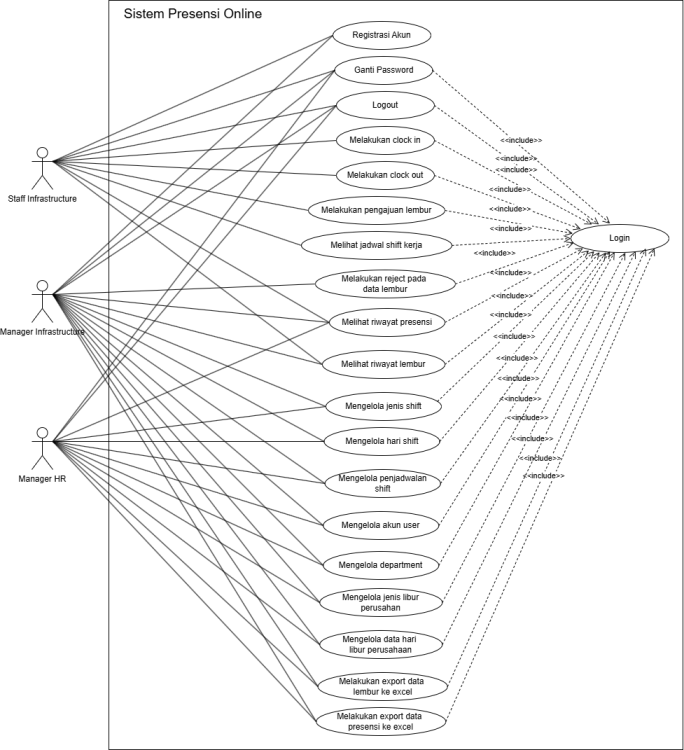
\includegraphics[width=13cm]{Gambar/bab2/use-case-presensi-online.png}
	\caption{\textit{Use Case Diagram} Aplikasi Presensi \textit{Online}}
	\label{fig:use-case-diagram-aplikasi-presensi-online}
\end{figure}
% Kembali ke penomoran bab 3 setelah gambar ini
% \renewcommand{\thefigure}{\thechapter.\arabic{figure}}
% \setcounter{figure}{0} % Optional, jika ingin mengatur ulang
\end{landscape}

\nextappendix
\section*{Lampiran \theappendixletter: \textit{Use Case Scenario} Aplikasi Presensi \textit{Online} 
\label{sec:use-case-scenario-aplikasi-presensi-online}}
\addcontentsline{toc}{section}{Lampiran \theappendixletter: \textit{Use Case Scenario} Aplikasi Presensi \textit{Online}}
\begin{longtable}{ |p{6cm}|p{8cm}|}
\caption{\textit{Use Case Scenario} Registrasi Akun}\label{tab:use-case-scenario-registrasi-akun} 
\\
\hline
\textbf{\textit{Use Case Name}}
&Registrasi Akun 
\\ \hline

\textbf{\textit{Actor}}
&\textit{Staff Infrastructure}, \textit{Manager Infrastructure} 
\\ \hline

\textbf{\textit{Brief Description}}
&\textit{Actor} yang tidak memiliki akun untuk \textit{login} dapat melakukan registrasi akun
\\ \hline

\textbf{\textit{Entry Conditions}}
&\textit{Actor} telah mengakses menu registrasi akun
\\ \hline

\textbf{\textit{Flow of event}}
&1. \textit{Actor} membuka menu registasi akun
\newline
2. \textit{Actor} mengisi seluruh \textit{form input} regitrasi akun dan menekan tombol \textit{submit}
\newline
3. Sistem menampilkan \textit{modal} verifikasi \textit{email} dan mengirimkan kode OTP ke \textit{email} \textit{actor}
\newline
4. \textit{Actor} mengisi kode OTP yang didapatkan melalui \textit{email}
\newline
5. \textit{Actor} menunggu akun diaktifkan oleh \textit{Manager}
\\ \hline

\textbf{\textit{Alternative scenario}}
&\textit{Actor} mengisi \textit{input email} pada \textit{form registrasi} dengan \textit{email} selain domain perusahaan dan sudah terdaftar maka : Sistem menampilkan pesan error
\\ \hline

\textbf{\textit{Exit Conditions}}
&Sistem menampilkan menu \textit{login}
\\ \hline
\end{longtable}

%%%%%%%%%%%%%%%%%%%%%%%%%%%%%%%%%%%%%%%%%%%%%%%%
\begin{longtable}{ |p{6cm}|p{8cm}|}
\caption{\textit{Use Case Scenario} Ganti Password}\label{tab:use-case-scenario-ganti-password} 
\\
\hline
\textbf{\textit{Use Case Name}}
&Ganti Password
\\ \hline

\textbf{\textit{Actor}}
&\textit{Staff Infrastructure}, \textit{Manager Infrastructure}, \textit{Manager Human Resources}
\\ \hline

\textbf{\textit{Brief Description}}
&\textit{Actor} yang ingin mengganti password akun
\\ \hline

\textbf{\textit{Entry Conditions}}
&\textit{Actor} telah melakukan \textit{login}
\\ \hline

\textbf{\textit{Flow of event}}
&1. \textit{Actor} membuka menu profil dan menekan tombol \textit{change password}
\newline
2. \textit{Actor} mengisi seluruh \textit{form input} pergantian password dan menekan tombol \textit{submit}
\newline
\\ \hline

\textbf{\textit{Alternative scenario}}
&\textit{Actor} yang salah mengisi password lama maka sistem akan mengembalikan pesan kesalahan
\\ \hline

\textbf{\textit{Exit Conditions}}
&Sistem selesai memproses pergantian passowrd dan menampilkan pesan berhasil ganti password
\\ \hline
\end{longtable}

%%%%%%%%%%%%%%%%%%%%%%%%%%%%%%%%%%%%%%%%%%%%%%%%%%%%%%%%%%%%%%%%%
\FloatBarrier
\begin{longtable}{ |p{6cm}|p{8cm}|}
\caption{\textit{Use Case Scenario Login}}\label{tab:use-case-scenario-login} 
\\
\hline
\textbf{\textit{Use Case Name}}
&\textit{Login}
\\ \hline

\textbf{\textit{Actor}}
&\textit{Staff Infrastructure}, \textit{Manager Infrastructure}, \textit{Manager Human Resources} 
\\ \hline

\textbf{\textit{Brief Description}}
&\textit{Actor} yang ingin masuk ke dalam menu utama dan menggunakan seluruh fitur didalam aplikasi
\\ \hline

\textbf{\textit{Entry Conditions}}
&\textit{Actor} yang telah melakukan regitrasi akun dan akun sudah berstatus aktif
\\ \hline

\textbf{\textit{Flow of event}}
&1. \textit{Actor} membuka halaman \textit{login}
\newline
2. \textit{Actor} mengisi seluruh \textit{form input} login dan menekan tombol \textit{login}
\newline
3. Sistem melakukan pengecekkan terhadap \textit{credential} dari \textit{user}
\newline
4. Sistem regenerasi \textit{session} pada \textit{user}
\\ \hline

\textbf{\textit{Alternative scenario}}
&1. \textit{Actor} yang salah mengisi \textit{form input email} atau \textit{password} maka: Sistem menampilkan pesan error
\newline
2. \textit{Actor} yang sudah \textit{login} sebelumnya dan sistem akan mengecek \textit{session} dari \textit{user}, kemudian mengarahkan \textit{user} ke halaman utama
\\ \hline

\textbf{\textit{Exit Conditions}}
&Sistem menampilkan menu utama dengan fitur yang sesuai masing-masing \textit{position} dan \textit{department}
\\ \hline
\end{longtable}

%%%%%%%%%%%%%%%%%%%%%%%%%%%%%%%%%%%%%%%%%%%%%%%%%%%%%%%%%%%%%%%%%
\FloatBarrier
\begin{longtable}{ |p{6cm}|p{8cm}|}
\caption{\textit{Use Case Scenario Logout}}\label{tab:use-case-scenario-logout} 
\\
\hline
\textbf{\textit{Use Case Name}}
&\textit{Logout}
\\ \hline

\textbf{\textit{Actor}}
&\textit{Staff Infrastructure}, \textit{Manager Infrastructure}, \textit{Manager Human Resources} 
\\ \hline

\textbf{\textit{Brief Description}}
&\textit{Actor} yang telah melakukan \textit{login} dan ingin keluar dari sesi \textit{login}
\\ \hline

\textbf{\textit{Entry Conditions}}
&\textit{Actor} yang sudah melakukan \textit{login}
\\ \hline

\textbf{\textit{Flow of event}}
&1. \textit{Actor} menekan tombol yang bergambar \textit{profile user} pada \textit{navbar}
\newline
2. Sistem akan menampilkan beberapa pilihan, \textit{actor} menekan pilihan \textit{logout}
\newline
3. Sistem akan melakukan \textit{logout} dan menghapus \textit{session} dari \textit{user}
\\ \hline

\textbf{\textit{Alternative scenario}}
&-
\\ \hline

\textbf{\textit{Exit Conditions}}
&Sistem menampilkan menu \textit{login}
\\ \hline
\end{longtable}

%%%%%%%%%%%%%%%%%%%%%%%%%%%%%%%%%%%%%%%%%%%%%%%%%%%%%%%%%%%%%%%%%
\FloatBarrier
\begin{longtable}{ |p{6cm}|p{8cm}|}
\caption{\textit{Use Case Scenario Melakukan Clock In}}\label{tab:use-case-scenario-clock-in} 
\\
\hline
\textbf{\textit{Use Case Name}}
&\textit{Melakukan clock In}
\\ \hline

\textbf{\textit{Actor}}
&\textit{Staff Infrastructure}
\\ \hline

\textbf{\textit{Brief Description}}
&\textit{Actor} yang melakukan presensi masuk
\\ \hline

\textbf{\textit{Entry Conditions}}
&\textit{Actor} yang sudah melakukan \textit{login} dan belum melakukan \textit{clock in} sebelumnya
\\ \hline

\textbf{\textit{Flow of event}}
&1. \textit{Actor} menekan tombol \textit{presence} pada navbar
\newline
2. Sistem akan tampilan halaman \textit{presence}
\newline
3. \textit{Actor} menekan tombol \textit{clock in}
\newline
4. Sistem akan menampikan \textit{pop up modal} yang berisi tombol untuk pengambilan lokasi dan foto
\newline
5. \textit{Actor} menekan tombol \textit{get my location} untuk meng-\textit{input} lokasi \textit{user} secara otomatis melalui GPS dan \textit{Actor} menekan tombol \textit{take photo} untuk membuka kamera dan melakukan pengambilan foto
\newline
6. Mengisi \textit{form input} informasi presensi , kemudian menekan tombol \textit{clock in now}
\newline
7. Sistem akan menyimpan data presensi \textit{actor}
\\ \hline

\textbf{\textit{Alternative scenario}}
&\textit{Actor} yang sudah melakukan \textit{clock in} saat terakhir kali maka : tombol \textit{clock in} akan ter-\textit{disabled}
\\ \hline

\textbf{\textit{Exit Conditions}}
&Sistem selesai memproses data presensi masuk dan menampilkan \textit{pop up message} berhasil \textit{clock in}
\\ \hline
\end{longtable}


%%%%%%%%%%%%%%%%%%%%%%%%%%%%%%%%%%%%%%%%%%%%%%%%%%%%%%%%%%%%%%%%%
\FloatBarrier
\begin{longtable}{ |p{6cm}|p{8cm}|}
\caption{\textit{Use Case Scenario} Melakukan \textit{Clock Out}}\label{tab:use-case-scenario-clock-out} 
\\
\hline
\textbf{\textit{Use Case Name}}
&Melakukan \textit{clock Out}
\\ \hline

\textbf{\textit{Actor}}
&\textit{Staff Infrastructure}
\\ \hline

\textbf{\textit{Brief Description}}
&\textit{Actor} yang melakukan presensi keluar
\\ \hline

\textbf{\textit{Entry Conditions}}
&\textit{Actor} yang sudah melakukan \textit{login} dan sudah melakukan \textit{clock in} sebelumnya
\\ \hline

\textbf{\textit{Flow of event}}
&1. \textit{Actor} menekan tombol \textit{presence} pada navbar
\newline
2. Sistem akan tampilan halaman \textit{presence}
\newline
3. \textit{Actor} menekan tombol \textit{clock out}
\newline
4. Sistem akan menampikan \textit{pop up modal} yang berisi tombol untuk pengambilan lokasi dan foto
\newline
5. \textit{Actor} menekan tombol \textit{get my location} untuk meng-\textit{input} lokasi \textit{user} secara otomatis melalui GPS dan \textit{Actor} menekan tombol \textit{take photo} untuk membuka kamera dan melakukan pengambilan foto
\newline
6. Mengisi \textit{input form} informasi presensi, kemudian menekan tombol \textit{clock out now}
\newline
7. Sistem akan menyimpan data presensi \textit{actor}, dan sistem akan mengecek pada data presensi saat \textit{clock in} dan \textit{clock out} dan menyimpan data lembur jika presensi dilakukan diluar jam \textit{shift} kerja atau hari libur
\newline
8. Jika terdapat data lembur, sistem menyimpan data lembur
\\ \hline

\textbf{\textit{Alternative scenario}}
&\textit{Actor} yang belum melakukan \textit{clock in} saat terakhir kali maka : tombol \textit{clock out} akan ter-\textit{disabled}
\\ \hline

\textbf{\textit{Exit Conditions}}
&Sistem selesai memproses data presensi keluar dan data lembur, kemudian menampilkan \textit{pop up message} berhasil \textit{clock out}
\\ \hline
\end{longtable}


%%%%%%%%%%%%%%%%%%%%%%%%%%%%%%%%%%%%%%%%%%%%%%%%%%%%%%%%%%%%%%%%%
\FloatBarrier
\begin{longtable}{ |p{6cm}|p{8cm}|}
\caption{\textit{Use Case Scenario} Melakukan Pengajuan Lembur}\label{tab:use-case-scenario-melakukan-pengajuan-lembur} 
\\
\hline
\textbf{\textit{Use Case Name}}
&Melakukan pengajuan lembur
\\ \hline

\textbf{\textit{Actor}}
&\textit{Staff Infrastructure}
\\ \hline

\textbf{\textit{Brief Description}}
&\textit{Actor} yang melakukan pengajuan lembur
\\ \hline

\textbf{\textit{Entry Conditions}}
&\textit{Actor} yang sudah melakukan \textit{login} dan ingin mengajukan lembur karena lupa presensi saat jam lembur
\\ \hline

\textbf{\textit{Flow of event}}
&1. \textit{Actor} menekan tombol \textit{request} pada navbar
\newline
2. Sistem akan menampilkan halaman \textit{overtime correction request}
\newline
3. \textit{Actor} mengisi seluruh \textit{form input} pada halaman \textit{overtime correction request} dan menekan tombol submit
\newline
4. Sistem akan menyimpan data lembur yang telah diisi oleh \textit{actor}
\\ \hline

\textbf{\textit{Alternative scenario}}
&\textit{Actor} yang tidak mengisi seluruh \textit{input form} maka : Sistem akan memberikan pesan error
\\ \hline

\textbf{\textit{Exit Conditions}}
&Sistem selesai memproses data lembur dan menampilkan \textit{pop up message} berhasil dan mengembalikan tampilan ke halaman \textit{overtime correction request}
\\ \hline
\end{longtable}

%%%%%%%%%%%%%%%%%%%%%%%%%%%%%%%%%%%%%%%%%%%%%%%%%%%%%%%%%%%%%%%%%
\FloatBarrier
\begin{longtable}{ |p{6cm}|p{8cm}|}
\caption{\textit{Use Case Scenario} Melihat Jadwal \textit{Shift} Kerja}\label{tab:use-case-scenario-melihat-jadwal-shift-kerja} 
\\
\hline
\textbf{\textit{Use Case Name}}
&Melihat jadwal \textit{shift} kerja
\\ \hline

\textbf{\textit{Actor}}
&\textit{Staff Infrastructure}
\\ \hline

\textbf{\textit{Brief Description}}
&\textit{Actor} yang melihat jadwal \textit{shift} kerja
\\ \hline

\textbf{\textit{Entry Conditions}}
&\textit{Actor} yang sudah melakukan \textit{login} dan ingin melihat jadwal \textit{shift} kerja
\\ \hline

\textbf{\textit{Flow of event}}
&1. \textit{Actor} menekan tombol \textit{presence} pada \textit{navbar}
\newline
2. Sistem akan menampilkan halaman \textit{presence}
\newline
3. \textit{Actor} menekan tombol \textit{shift schedule}
\newline
4. Sistem akan menampilkan jadwal kerja \textit{actor}
\\ \hline

\textbf{\textit{Alternative scenario}}
&\textit{Actor} yang tidak memiliki jadwal kerja maka tidak akan ada data yang ditampilkan
\\ \hline

\textbf{\textit{Exit Conditions}}
&\textit{Actor} menutup \textit{modal} data \textit{shift} dan sistem menampilkan kembali halaman \textit{attendance}
\\ \hline
\end{longtable}

%%%%%%%%%%%%%%%%%%%%%%%%%%%%%%%%%%%%%%%%%%%%%%%%%%%%%%%%%%%%%%%%%
\FloatBarrier
\begin{longtable}{ |p{6cm}|p{8cm}|}
\caption{\textit{Use Case Scenario} Melakukan \textit{Reject} Pada Data Lembur}\label{tab:use-case-scenario-melakukan-approval} 
\\
\hline
\textbf{\textit{Use Case Name}}
&Melakukan \textit{reject} pada data lembur
\\ \hline

\textbf{\textit{Actor}}
&\textit{Manager Infrastructure}
\\ \hline

\textbf{\textit{Brief Description}}
&\textit{Actor} yang melakukan \textit{reject} pada data lembur
\\ \hline

\textbf{\textit{Entry Conditions}}
&\textit{Actor} yang sudah melakukan \textit{login} dan ingin melakukan penolakkan atau \textit{reject} pada data lembur yang masuk
\\ \hline

\textbf{\textit{Flow of event}}
&1. \textit{Actor} menekan tombol \textit{reject} pada \textit{navbar}
\newline
2. Sistem akan menampilkan \textit{list} data \textit{lembur} yang tidak pernah di-\textit{reject}
\newline
3. \textit{Actor} melakukan \textit{reject} pada data yang dipilih atau mencetang \textit{checkbox} pada data lembur dan menekan tombol \textit{reject selected}
\newline
5. \textit{Actor} melakukan konfirmasi perubahan
\newline
6. Sistem menyimpan perubahan data
\\ \hline

\textbf{\textit{Alternative scenario}}
&-
\\ \hline

\textbf{\textit{Exit Conditions}}
&Sistem selesai memproses seluruh perubahan data lembur dan kembali menampilkan halaman \textit{reject}
\\ \hline
\end{longtable}

%%%%%%%%%%%%%%%%%%%%%%%%%%%%%%%%%%%%%%%%%%%%%%%%%%%%%%%%%%%%%%%%%
\FloatBarrier
\begin{longtable}{ |p{6cm}|p{8cm}|}
\caption{\textit{Use Case Scenario} Melakukan \textit{Export} Data Lembur ke \textit{Excel}}\label{tab:use-case-scenario-melakukan-export-data-lembur} 
\\
\hline
\textbf{\textit{Use Case Name}}
&Melakukan \textit{Export} Data Lembur ke \textit{Excel}
\\ \hline

\textbf{\textit{Actor}}
&\textit{Manager Human Resources, Manager Infrastructure}
\\ \hline

\textbf{\textit{Brief Description}}
&\textit{Actor} yang melakukan \textit{export} data lembur menjadi format \textit{Excel}
\\ \hline

\textbf{\textit{Entry Conditions}}
&\textit{Actor} yang sudah melakukan \textit{login} dan ingin melakukan \textit{export} data lembur menjadi format \textit{Excel}
\\ \hline

\textbf{\textit{Flow of event}}
&1. \textit{Actor} menekan tombol \textit{overtime history} pada \textit{navbar}
\newline
2. Sistem akan menampilkan \textit{list} data riwayat lembur
\newline
3. \textit{Actor} melakukan \textit{filter} nama \textit{staff}, tanggal atau status
\newline
4. Sistem menampilkan data lembur yang telah di-\textit{filter}
\newline
5. \textit{Actor} menekan tombol \textit{Export}
\newline
6. Sistem akan memproses data lembur dan memberikan konfirmasi untuk men-\textit{download} \textit{file} dalam bentu \textit{Excel}
\newline
7. \textit{Actor} mengunduh \textit{file Excel}
\newline
\\ \hline

\textbf{\textit{Alternative scenario}}
&Jika tidak ada data lembur atau data yang di-\textit{filter} tidak ditemukan, maka sistem tidak akan memproses permintaan \textit{export}
\\ \hline

\textbf{\textit{Exit Conditions}}
&\textit{Actor} menekan konfirmasi saat pengunduhan \textit{file} dan sistem akan mengembalikan tampilan ke \textit{overtime history}
\\ \hline
\end{longtable}

%%%%%%%%%%%%%%%%%%%%%%%%%%%%%%%%%%%%%%%%%%%%%%%%%%%%%%%%%%%%%%%%%
\FloatBarrier
\begin{longtable}{ |p{6cm}|p{8cm}|}
\caption{\textit{Use Case Scenario} Melakukan \textit{Export} Data Presensi ke \textit{Excel}}\label{tab:use-case-scenario-melakukan-export-data-presensi} 
\\
\hline
\textbf{\textit{Use Case Name}}
&Melakukan \textit{Export} Data Presensi ke \textit{Excel}
\\ \hline

\textbf{\textit{Actor}}
&\textit{Manager Human Resources, Manager Infrastructure}
\\ \hline

\textbf{\textit{Brief Description}}
&\textit{Actor} yang melakukan \textit{export} data presensi menjadi format \textit{Excel}
\\ \hline

\textbf{\textit{Entry Conditions}}
&\textit{Actor} yang sudah melakukan \textit{login} dan ingin melakukan \textit{export} data presensi menjadi format \textit{Excel}
\\ \hline

\textbf{\textit{Flow of event}}
&1. \textit{Actor} menekan tombol \textit{attendance history} pada \textit{navbar}
\newline
2. Sistem akan menampilkan \textit{list} data riwayat presensi
\newline
3. \textit{Actor} melakukan \textit{filter} nama \textit{staff}, tanggal atau status
\newline
4. Sistem menampilkan data presensi yang telah di-\textit{filter}
\newline
5. \textit{Actor} menekan tombol \textit{Export}
\newline
6. Sistem akan memproses data presensi dan memberikan konfirmasi untuk men-\textit{download} \textit{file} dalam bentu \textit{Excel}
\newline
7. \textit{Actor} mengunduh \textit{file Excel}
\newline
\\ \hline

\textbf{\textit{Alternative scenario}}
&Jika tidak ada data presensi atau data yang di-\textit{filter} tidak ditemukan, maka sistem tidak akan memproses permintaan \textit{export}
\\ \hline

\textbf{\textit{Exit Conditions}}
&\textit{Actor} menekan konfirmasi saat pengunduhan \textit{file} dan sistem akan mengembalikan tampilan ke \textit{attendance history}
\\ \hline
\end{longtable}

%%%%%%%%%%%%%%%%%%%%%%%%%%%%%%%%%%%%%%%%%%%%%%%%%%%%%%%%%%%%%%%%%
\FloatBarrier
\begin{longtable}{ |p{6cm}|p{8cm}|}
\caption{\textit{Use Case Scenario} Melihat Riwayat Lembur}\label{tab:use-case-scenario-melihat-riwayat-lembur} 
\\
\hline
\textbf{\textit{Use Case Name}}
&Melihat riwayat lembur
\\ \hline

\textbf{\textit{Actor}}
&\textit{Staff Infrastructure}, \textit{Manager Infrastructure}, \textit{Manager Human Resources}
\\ \hline

\textbf{\textit{Brief Description}}
&\textit{Actor} yang melihat riwayat lembur
\\ \hline

\textbf{\textit{Entry Conditions}}
&\textit{Actor} yang sudah melakukan \textit{login} dan ingin melihat riwayat lembur
\\ \hline

\textbf{\textit{Flow of event}}
&1. \textit{Actor} menekan tombol \textit{overtime history} pada \textit{navbar}
\newline
2. Sistem akan menampilkan \textit{list} data riwayat lembur
\newline
3. \textit{Actor} melakukan \textit{filter} tanggal dan status pada data lembur untuk mencari spesifik data lembur
\newline
4. \textit{Actor} menekan tombol \textit{details} pada salah satu data lembur
\newline
5. Sistem menampilkan halaman \textit{details} dan informasi lengkap terkait data lembur yang dipilih
\newline
\\ \hline

\textbf{\textit{Alternative scenario}}
&Jika tidak ada data lembur atau data yang di-\textit{filter} tidak ditemukan, maka sistem tidak akan menampilkan data
\\ \hline

\textbf{\textit{Exit Conditions}}
&\textit{Actor} menekan tombol kembali dan sistem akan menampilkan kembali halaman \textit{overtime history}
\\ \hline
\end{longtable}

%%%%%%%%%%%%%%%%%%%%%%%%%%%%%%%%%%%%%%%%%%%%%%%%%%%%%%%%%%%%%%%%%
\FloatBarrier
\begin{longtable}{ |p{6cm}|p{8cm}|}
\caption{\textit{Use Case Scenario} Melihat Riwayat Presensi}\label{tab:use-case-scenario-melihat-riwayat-presensi} 
\\
\hline
\textbf{\textit{Use Case Name}}
&Melihat riwayat presensi
\\ \hline

\textbf{\textit{Actor}}
&\textit{Staff Infrastructure}, \textit{Manager Infrastructure}, \textit{Manager Human Resources}
\\ \hline

\textbf{\textit{Brief Description}}
&\textit{Actor} yang melihat riwayat presensi
\\ \hline

\textbf{\textit{Entry Conditions}}
&\textit{Actor} yang sudah melakukan \textit{login} dan ingin melihat riwayat presensi
\\ \hline

\textbf{\textit{Flow of event}}
&1. \textit{Actor} menekan tombol \textit{attendance history} pada \textit{navbar}
\newline
2. Sistem akan menampilkan \textit{list} data riwayat presensi
\newline
3. \textit{Actor} melakukan \textit{filter} tanggal pada data presensi untuk mencari spesifik data presensi
\newline
4. \textit{Actor} menekan tombol \textit{details} pada salah satu data presensi
\newline
5. Sistem menampilkan halaman \textit{details} dan informasi lengkap terkait data presensi yang dipilih
\newline
\\ \hline

\textbf{\textit{Alternative scenario}}
&Jika tidak ada data presensi atau data yang di-\textit{filter} tidak ditemukan, maka sistem tidak akan menampilkan data
\\ \hline

\textbf{\textit{Exit Conditions}}
&\textit{Actor} menekan tombol kembali dan sistem akan menampilkan kembali halaman \textit{attendance history}
\\ \hline
\end{longtable}

%%%%%%%%%%%%%%%%%%%%%%%%%%%%%%%%%%%%%%%%%%%%%%%%%%%%%%%%%%%%%%%%%
\FloatBarrier
\begin{longtable}{ |p{6cm}|p{8cm}|}
\caption{\textit{Use Case Scenario} Mengelola Jenis \textit{Shift}}\label{tab:use-case-scenario-mengelola-jenis-shift} 
\\
\hline
\textbf{\textit{Use Case Name}}
&Mengelola jenis \textit{shift}
\\ \hline

\textbf{\textit{Actor}}
&\textit{Manager Human Resources}, \textit{Manager Infrastructure}
\\ \hline

\textbf{\textit{Brief Description}}
&\textit{Actor} yang mengelola jenis \textit{shift}
\\ \hline

\textbf{\textit{Entry Conditions}}
&\textit{Actor} yang sudah melakukan \textit{login} dan ingin mengelola jenis \textit{shift}
\\ \hline

\textbf{\textit{Flow of event}}
&1. \textit{Actor} menekan tombol \textit{shift} pada \textit{navbar}
\newline
2. Sistem akan menampilkan halaman \textit{shift} beserta data jenis \textit{shift} kerja
\newline
3. \textit{Actor} mengelola (\textit{create, update, delete}) data jenis \textit{shift}
    \newline
4. Sistem menampilkan konfirmasi perubahan data
\newline
5. \textit{Actor} melakukan konfirmasi perubahan
\newline
6. Sistem menyimpan perubahan data
\newline
\\ \hline

\textbf{\textit{Alternative scenario}}
&\textit{Actor} yang tidak melakukan konfirmasi perubahan data maka sistem tidak akan menyimpan perubahan data
\\ \hline

\textbf{\textit{Exit Conditions}}
&Sistem selesai memproses seluruh perubahan data jenis \textit{shift} dan kembali menampilkan halaman \textit{shift}
\\ \hline
\end{longtable}

%%%%%%%%%%%%%%%%%%%%%%%%%%%%%%%%%%%%%%%%%%%%%%%%%%%%%%%%%%%%%%%%%
\FloatBarrier
\begin{longtable}{ |p{6cm}|p{8cm}|}
\caption{\textit{Use Case Scenario} Mengelola Hari \textit{Shift}}\label{tab:use-case-scenario-mengelola-hari-shift} 
\\
\hline
\textbf{\textit{Use Case Name}}
&Mengelola hari \textit{shift}
\\ \hline

\textbf{\textit{Actor}}
&\textit{Manager Human Resources}, \textit{Manager Infrastructure}
\\ \hline

\textbf{\textit{Brief Description}}
&\textit{Actor} yang mengelola hari \textit{shift}
\\ \hline

\textbf{\textit{Entry Conditions}}
&\textit{Actor} yang sudah melakukan \textit{login} dan ingin mengelola hari \textit{shift}
\\ \hline

\textbf{\textit{Flow of event}}
&1. \textit{Actor} menekan \textit{edit} pada salah satu jenis \textit{shift} melalui halaman \textit{shift}
\newline
2. Sistem akan menampilkan \textit{modal} hari \textit{shift} beserta data hari \textit{shift} kerja
\newline
3. \textit{Actor} mengelola (\textit{create, update, delete}) data hari \textit{shift}
    \newline
4. Sistem menampilkan konfirmasi perubahan data
\newline
5. \textit{Actor} melakukan konfirmasi perubahan
\newline
6. Sistem menyimpan perubahan data
\newline
\\ \hline

\textbf{\textit{Alternative scenario}}
&\textit{Actor} yang tidak melakukan konfirmasi perubahan data maka sistem tidak akan menyimpan perubahan data
\\ \hline

\textbf{\textit{Exit Conditions}}
&Sistem selesai memproses seluruh perubahan data hari \textit{shift} dan kembali menampilkan halaman \textit{shift}
\\ \hline
\end{longtable}

%%%%%%%%%%%%%%%%%%%%%%%%%%%%%%%%%%%%%%%%%%%%%%%%%%%%%%%%%%%%%%%%%
\FloatBarrier
\begin{longtable}{ |p{6cm}|p{8cm}|}
\caption{\textit{Use Case Scenario} Mengelola Penjadwalan \textit{Shift}}\label{tab:use-case-scenario-mengelola-penjadwalan-shift}
\\
\hline
\textbf{\textit{Use Case Name}}
&Mengelola penjadwalan \textit{shift}
\\ \hline

\textbf{\textit{Actor}}
&\textit{Manager Human Resources}, \textit{Manager Infrastructure}
\\ \hline

\textbf{\textit{Brief Description}}
&\textit{Actor} yang mengelola penjadwalan \textit{shift}
\\ \hline

\textbf{\textit{Entry Conditions}}
&\textit{Actor} yang sudah melakukan \textit{login} dan ingin mengelola penjadwalan \textit{shift}
\\ \hline

\textbf{\textit{Flow of event}}
&1. \textit{Actor} menekan tombol \textit{shift scheduling} pada \textit{navbar}
\newline
2. Sistem akan menampilkan halaman penjadwalan \textit{shift} beserta data penjadwalan \textit{shift} kerja
\newline
3. \textit{Actor} mengelola (\textit{create, update, delete, import}) data penjadwalan \textit{shift}
    \newline
4. Sistem menampilkan konfirmasi perubahan data
\newline
5. \textit{Actor} melakukan konfirmasi perubahan
\newline
6. Sistem menyimpan perubahan data
\newline
\\ \hline

\textbf{\textit{Alternative scenario}}
&\textit{Actor} yang tidak melakukan konfirmasi perubahan data maka sistem tidak akan menyimpan perubahan data
\\ \hline

\textbf{\textit{Exit Conditions}}
&Sistem selesai memproses seluruh perubahan data penjadwalan \textit{shift} dan kembali menampilkan halaman penjadwalan \textit{shift}
\\ \hline
\end{longtable}


%%%%%%%%%%%%%%%%%%%%%%%%%%%%%%%%%%%%%%%%%%%%%%%%%%%%%%%%%%%%%%%%%
\FloatBarrier
\begin{longtable}{ |p{6cm}|p{8cm}|}
\caption{\textit{Use Case Scenario} Mengelola Akun \textit{User}}\label{tab:use-case-scenario-mengelola-akun-user} 
\\
\hline
\textbf{\textit{Use Case Name}}
&Mengelola akun \textit{user}
\\ \hline

\textbf{\textit{Actor}}
&\textit{Manager Human Resources}, \textit{Manager Infrastructure}
\\ \hline

\textbf{\textit{Brief Description}}
&\textit{Actor} yang mengelola akun \textit{user}
\\ \hline

\textbf{\textit{Entry Conditions}}
&\textit{Actor} yang sudah melakukan \textit{login} dan ingin mengelola akun \textit{user}
\\ \hline

\textbf{\textit{Flow of event}}
&1. \textit{Actor} menekan tombol \textit{user} pada \textit{navbar}
\newline
2. Sistem akan menampilkan halaman \textit{user} beserta data semua \textit{user}
\newline
3. \textit{Actor} mengelola \textit{update, delete} data akun \textit{user}
\newline
4. Sistem menampilkan konfirmasi perubahan data
\newline
5. \textit{Actor} melakukan konfirmasi perubahan
\newline
6. Sistem menyimpan perubahan data
\\ \hline

\textbf{\textit{Alternative scenario}}
&\textit{Actor} yang tidak melakukan konfirmasi perubahan data maka sistem tidak akan menyimpan perubahan data
\\ \hline

\textbf{\textit{Exit Conditions}}
&Sistem selesai memproses seluruh perubahan data \textit{user} dan kembali menampilkan halaman \textit{user}
\\ \hline
\end{longtable}

%%%%%%%%%%%%%%%%%%%%%%%%%%%%%%%%%%%%%%%%%%%%%%%%%%%%%%%%%%%%%%%%%
\FloatBarrier
\begin{longtable}{ |p{6cm}|p{8cm}|}
\caption{\textit{Use Case Scenario} Mengelola \textit{Department}}\label{tab:use-case-scenario-mengelola-department} 
\\
\hline
\textbf{\textit{Use Case Name}}
&Mengelola \textit{department}
\\ \hline

\textbf{\textit{Actor}}
&\textit{Manager Human Resources}, \textit{Manager Infrastructure}
\\ \hline

\textbf{\textit{Brief Description}}
&\textit{Actor} yang mengelola \textit{department}
\\ \hline

\textbf{\textit{Entry Conditions}}
&\textit{Actor} yang sudah melakukan \textit{login} dan ingin mengelola \textit{department}
\\ \hline

\textbf{\textit{Flow of event}}
&1. \textit{Actor} menekan tombol \textit{department} pada \textit{navbar}
\newline
2. Sistem akan menampilkan halaman \textit{department} beserta data semua \textit{department}
\newline
3. \textit{Actor} mengelola \textit{update, delete} data akun \textit{department}
\newline
4. Sistem menampilkan konfirmasi perubahan data
\newline
5. \textit{Actor} melakukan konfirmasi perubahan
\newline
6. Sistem menyimpan perubahan data
\\ \hline

\textbf{\textit{Alternative scenario}}
&\textit{Actor} yang tidak melakukan konfirmasi perubahan data maka sistem tidak akan menyimpan perubahan data
\\ \hline

\textbf{\textit{Exit Conditions}}
&Sistem selesai memproses seluruh perubahan data \textit{department} dan kembali menampilkan halaman \textit{department}
\\ \hline
\end{longtable}

%%%%%%%%%%%%%%%%%%%%%%%%%%%%%%%%%%%%%%%%%%%%%%%%%%%%%%%%%%%%%%%%%
\FloatBarrier
\begin{longtable}{ |p{6cm}|p{8cm}|}
\caption{\textit{Use Case Scenario} Mengelola Jenis Libur Perusahaan}\label{tab:use-case-scenario-mengelola-jenis-libur-perusahaan} 
\\
\hline
\textbf{\textit{Use Case Name}}
&Mengelola jenis libur perusahaan
\\ \hline

\textbf{\textit{Actor}}
&\textit{Manager Human Resources}, \textit{Manager Infrastructure}
\\ \hline

\textbf{\textit{Brief Description}}
&\textit{Actor} yang mengelola jenis libur perusahaan
\\ \hline

\textbf{\textit{Entry Conditions}}
&\textit{Actor} yang sudah melakukan \textit{login} dan ingin mengelola jenis libur perusahaan
\\ \hline

\textbf{\textit{Flow of event}}
&1. \textit{Actor} menekan tombol libur pada \textit{navbar}
\newline
2. Sistem akan menampilkan halaman libur beserta seluruh data jenis libur perusahaan
\newline
3. \textit{Actor} mengelola (\textit{create, update, delete}) data jenis libur perusahaan
\newline
4. Sistem menampilkan konfirmasi perubahan data
\newline
5. \textit{Actor} melakukan konfirmasi perubahan
\newline
6. Sistem menyimpan perubahan data
\\ \hline

\textbf{\textit{Alternative scenario}}
&1. \textit{Actor} yang tidak melakukan konfirmasi perubahan data maka sistem tidak akan menyimpan perubahan data
\newline
2. Jika tidak ada data hari libur yang ditemukan, maka sistem tidak akan menampilkan hasil
\\ \hline

\textbf{\textit{Exit Conditions}}
&Sistem selesai memproses seluruh perubahan data jenis libur perusahaan dan kembali menampilkan halaman jenis libur
\\ \hline
\end{longtable}

%%%%%%%%%%%%%%%%%%%%%%%%%%%%%%%%%%%%%%%%%%%%%%%%%%%%%%%%%%%%%%%%%
\FloatBarrier
\begin{longtable}{ |p{6cm}|p{8cm}|}
\caption{\textit{Use Case Scenario} Mengelola Data Hari Libur Perusahaan}\label{tab:use-case-scenario-mengelola-data-hari-libur-perusahaan} 
\\
\hline
\textbf{\textit{Use Case Name}}
&Mengelola data hari libur perusahaan
\\ \hline

\textbf{\textit{Actor}}
&\textit{Manager Human Resources}, \textit{Manager Infrastructure}
\\ \hline

\textbf{\textit{Brief Description}}
&\textit{Actor} yang mengelola data hari libur perusahaan
\\ \hline

\textbf{\textit{Entry Conditions}}
&\textit{Actor} yang sudah melakukan \textit{login} dan ingin mengelola data hari libur perusahaan
\\ \hline

\textbf{\textit{Flow of event}}
&1. \textit{Actor} menekan tombol edit pada jenis libur perusahaan
\newline
2. Sistem akan menampilkan halaman hari libur beserta seluruh data hari libur perusahaan
\newline
3. \textit{Actor} mengelola (\textit{create, update, delete}) data hari libur perusahaan atau \textit{import} data hari libur nasional melalui tombol yang terhubung dengan API
\newline
4. Sistem menampilkan konfirmasi perubahan data
\newline
5. \textit{Actor} melakukan konfirmasi perubahan
\newline
6. Sistem menyimpan perubahan data
\\ \hline

\textbf{\textit{Alternative scenario}}
&1. \textit{Actor} yang tidak melakukan konfirmasi perubahan data maka sistem tidak akan menyimpan perubahan data
\newline
2. Jika tidak ada data hari libur yang ditemukan, maka sistem tidak akan menampilkan hasil
\\ \hline

\textbf{\textit{Exit Conditions}}
&Sistem selesai memproses seluruh perubahan data hari libur perusahaan dan kembali menampilkan halaman hari libur
\\ \hline
\end{longtable}


\pagebreak

\nextappendix
\section*{Lampiran \theappendixletter: \textit{Activity Diagram} Aplikasi Presensi \textit{Online} 
\label{sec:activity-diagram-aplikasi-presensi-online}}
\addcontentsline{toc}{section}{Lampiran \theappendixletter: \textit{Activity Diagram} Aplikasi Presensi \textit{Online}}
\begin{figure}[H]
	\centering
	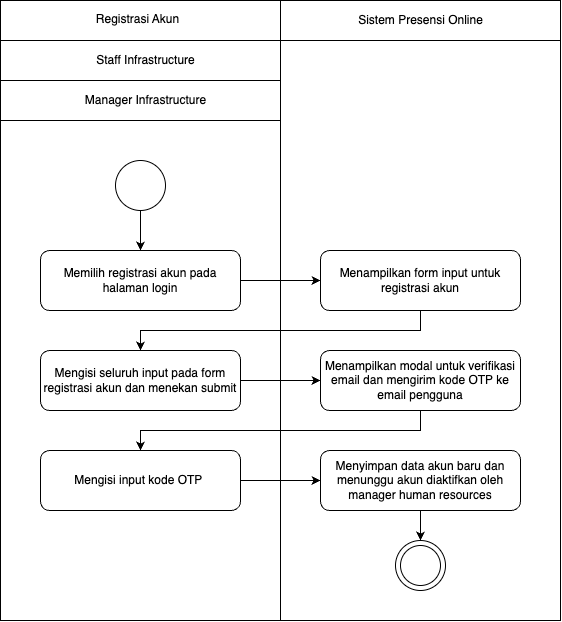
\includegraphics[width=15cm]{Gambar/bab2/activity-diagram-registrasi.png}
	\caption{\textit{Activity Diagram} Registrasi Akun}
	\label{fig:activity-diagram-registrasi}
\end{figure}
\FloatBarrier

\begin{figure}[H]
	\centering
	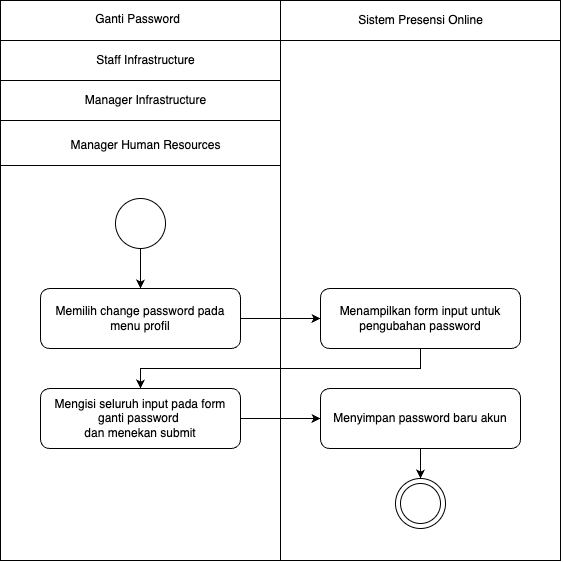
\includegraphics[width=15cm]{Gambar/bab2/activity-diagram-ganti-password.png}
	\caption{\textit{Activity Diagram} Ganti Password}
	\label{fig:activity-diagram-ganti-password}
\end{figure}
\FloatBarrier

\begin{figure}[H]
	\centering
	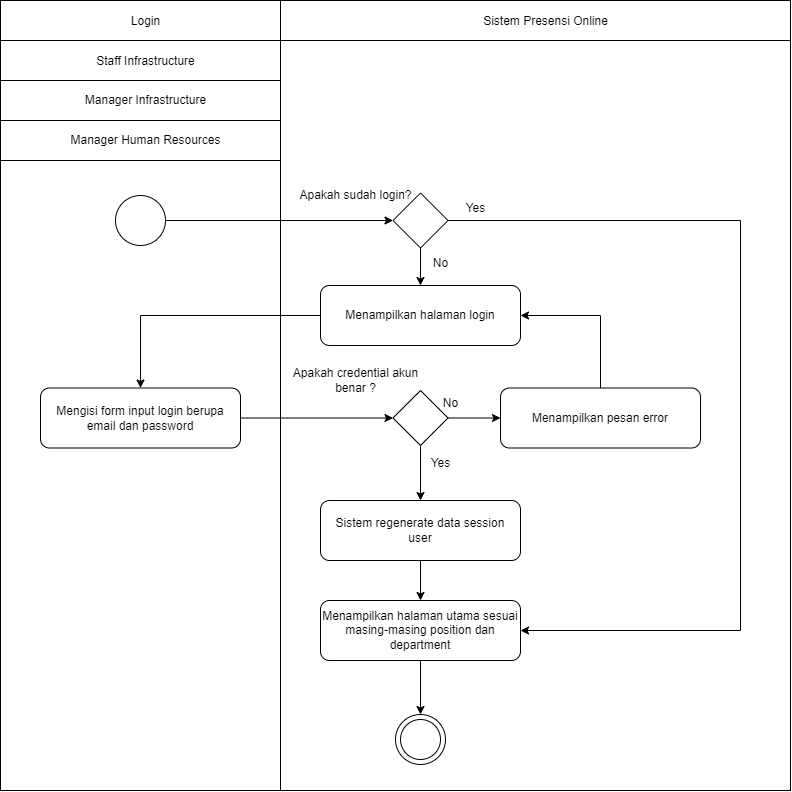
\includegraphics[width=15cm]{Gambar/bab2/activity-diagram-login.png}
	\caption{\textit{Activity Diagram Login}}
	\label{fig:activity-diagram-login}
\end{figure}
\FloatBarrier

\begin{figure}[H]
	\centering
	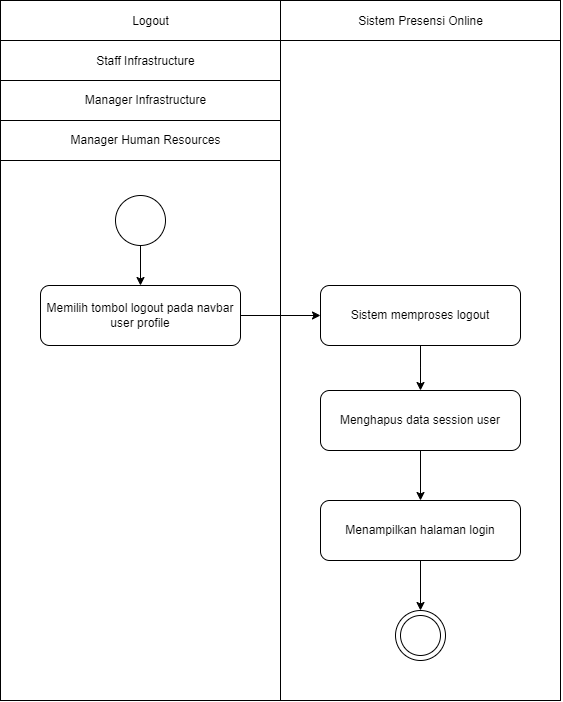
\includegraphics[width=15cm]{Gambar/bab2/activity-diagram-logout.png}
	\caption{\textit{Activity Diagram Logout}}
	\label{fig:activity-diagram-logout}
\end{figure}
\FloatBarrier

\begin{figure}[H]
	\centering
	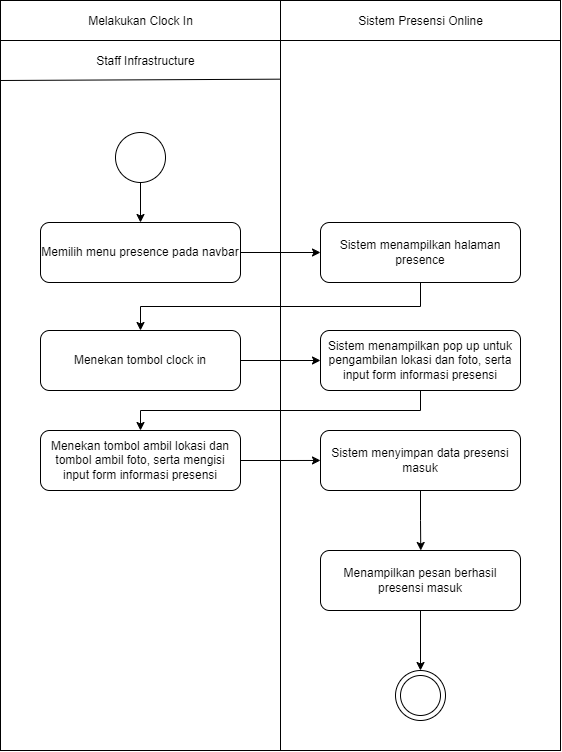
\includegraphics[width=17cm]{Gambar/bab2/activity-diagram-clock-in.png}
	\caption{\textit{Activity Diagram Clock In}}
	\label{fig:activity-diagram-clock-in}
\end{figure}
\FloatBarrier

\begin{figure}[H]
	\centering
	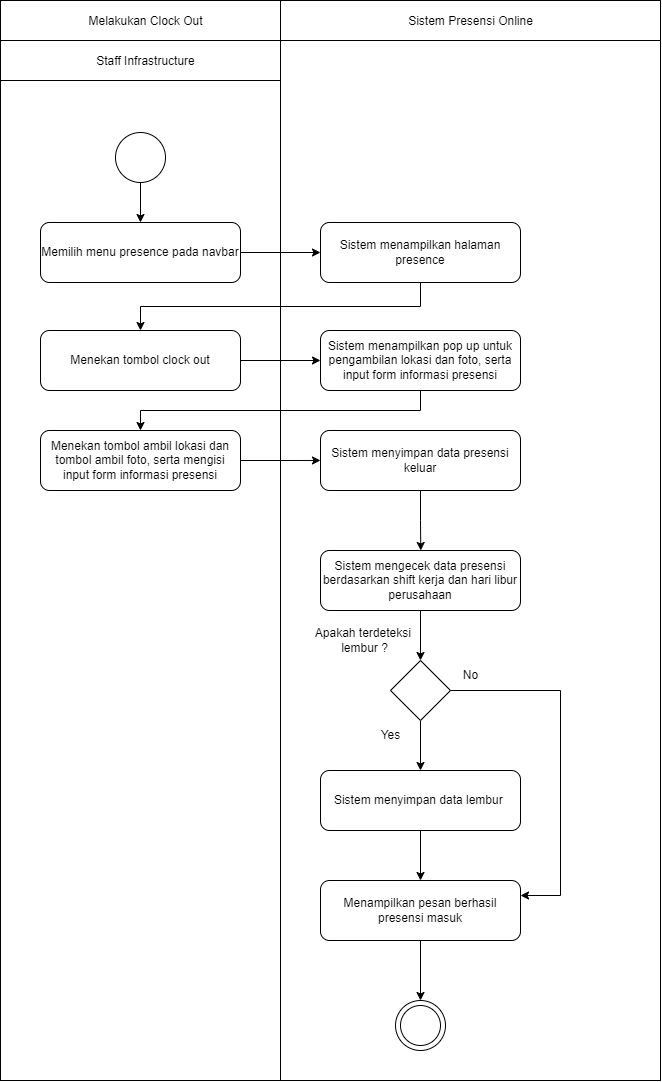
\includegraphics[width=13cm]{Gambar/bab2/activity-diagram-clock-out.png}
	\caption{\textit{Activity Diagram Clock Out}}
	\label{fig:activity-diagram-clock-out}
\end{figure}
\FloatBarrier

\begin{figure}[H]
	\centering
	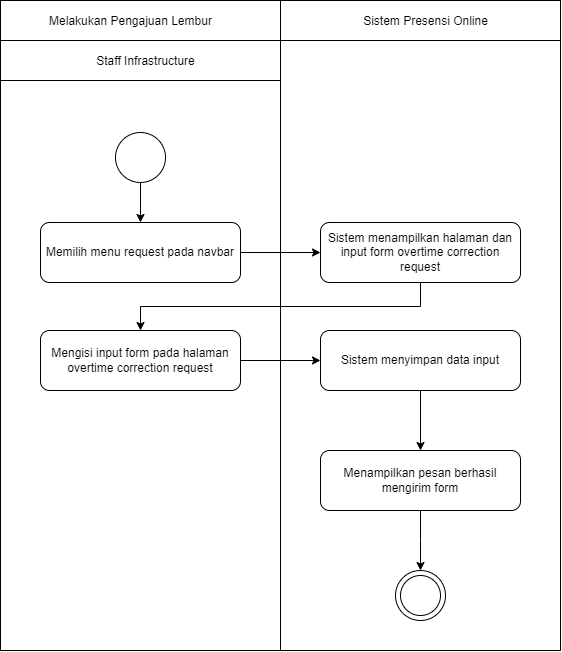
\includegraphics[width=15cm]{Gambar/bab2/activity-diagram-melakukan-pengajuan-lembur.png}
	\caption{\textit{Activity Diagram} Melakukan Pengajuan Lembur}
	\label{fig:activity-diagram-melakukan-pengajuan-lembur}
\end{figure}
\FloatBarrier

\begin{figure}[H]
	\centering
	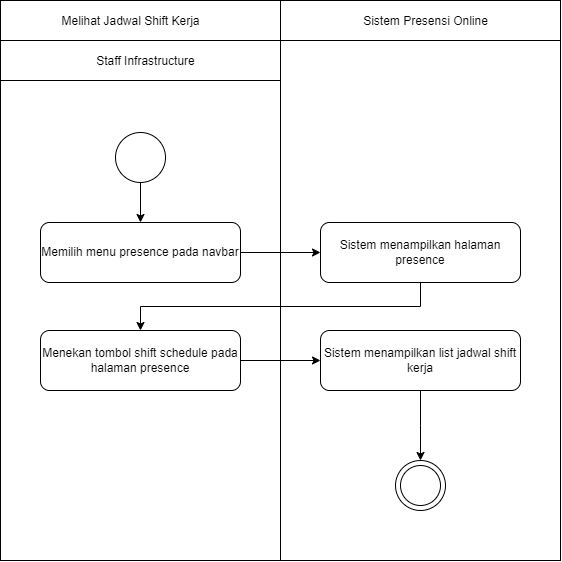
\includegraphics[width=15cm]{Gambar/bab2/activity-diagram-melihat-jadwal-shift-kerja.png}
	\caption{\textit{Activity Diagram} Melihat Jadwal \textit{Shift} Kerja}
	\label{fig:activity-diagram-melihat-jadwal-shift-kerja}
\end{figure}
\FloatBarrier

\begin{figure}[H]
	\centering
	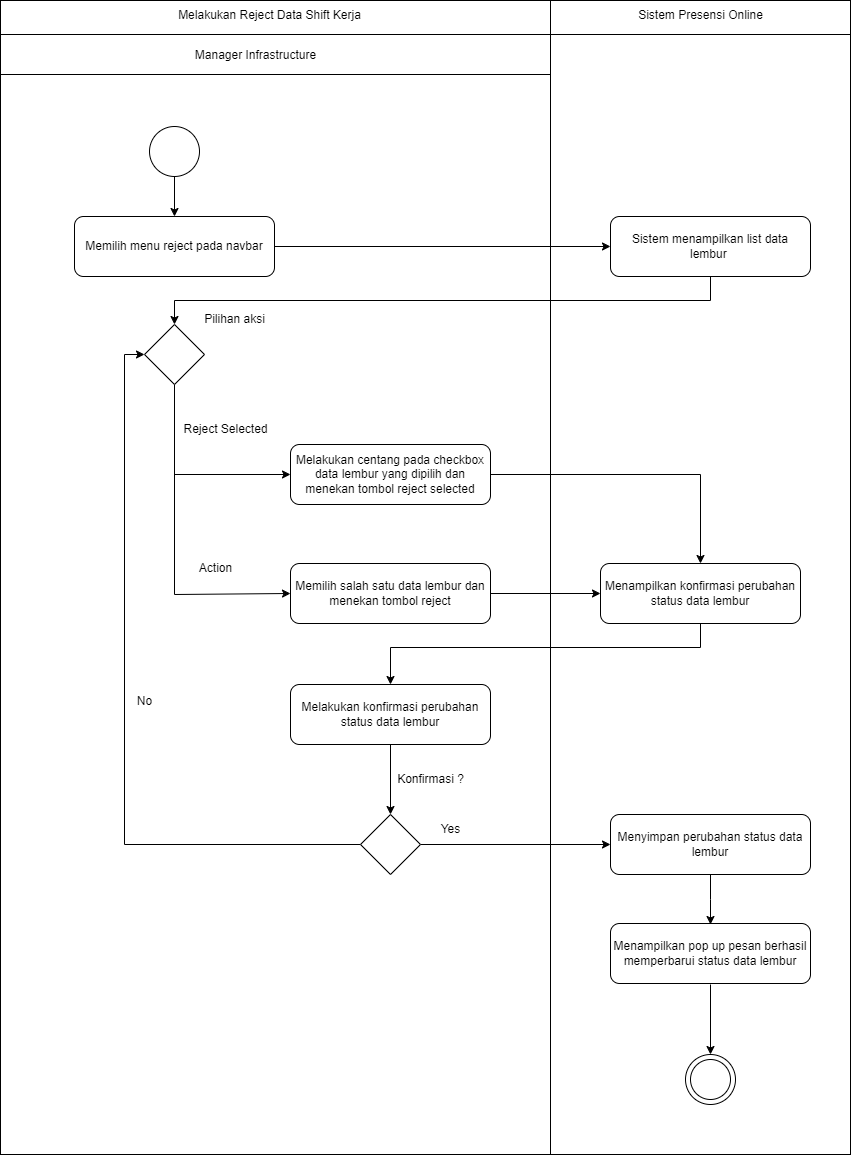
\includegraphics[width=14cm]{Gambar/bab2/activity-diagram-melakukan-reject.png}
	\caption{\textit{Activity Diagram} Melakukan \textit{Reject} pada Data Lembur}
	\label{fig:activity-diagram-melakukan-reject}
\end{figure}
\FloatBarrier

\begin{figure}[H]
	\centering
	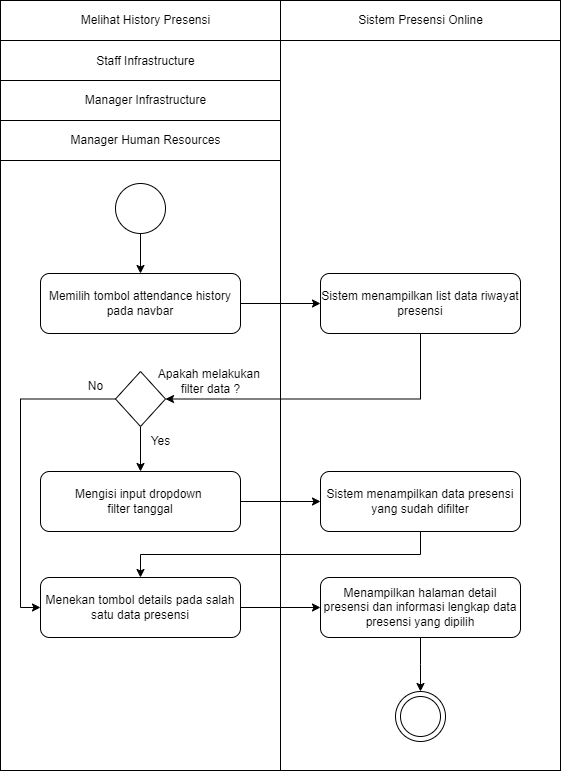
\includegraphics[width=15cm]{Gambar/bab2/activity-diagram-melihat-history-presensi.png}
	\caption{\textit{Activity Diagram} Melihat Riwayat Presensi}
	\label{fig:activity-diagram-melihat-riwayat-presensi}
\end{figure}
\FloatBarrier

\begin{figure}[H]
	\centering
	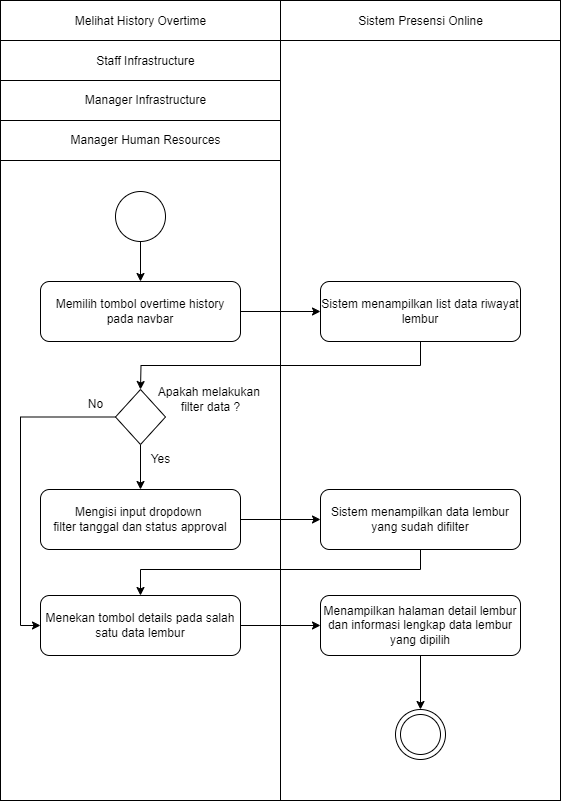
\includegraphics[width=15cm]{Gambar/bab2/activity-diagram-melihat-history-lembur.png}
	\caption{\textit{Activity Diagram} Melihat Riwayat Lembur}
	\label{fig:activity-diagram-melihat-riwayat-lembur}
\end{figure}
\FloatBarrier

\begin{figure}[H]
	\centering
	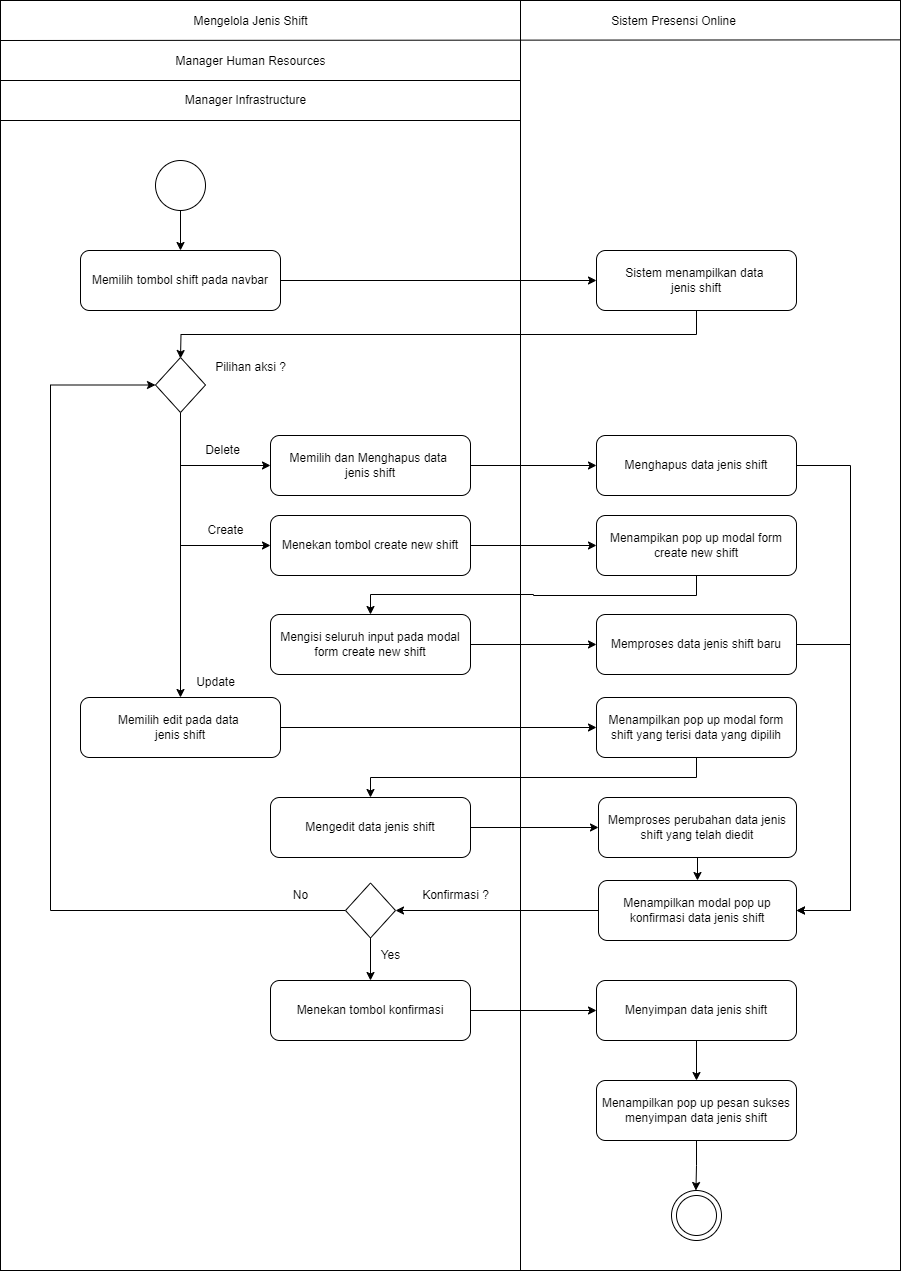
\includegraphics[width=15cm]{Gambar/bab2/activity-diagram-mengelola-data-jenis-shift.png}
	\caption{\textit{Activity Diagram} Mengelola Jenis \textit{Shift}}
	\label{fig:activity-diagram-mengelola-jenis-shift}
\end{figure}
\FloatBarrier

\begin{figure}[H]
	\centering
	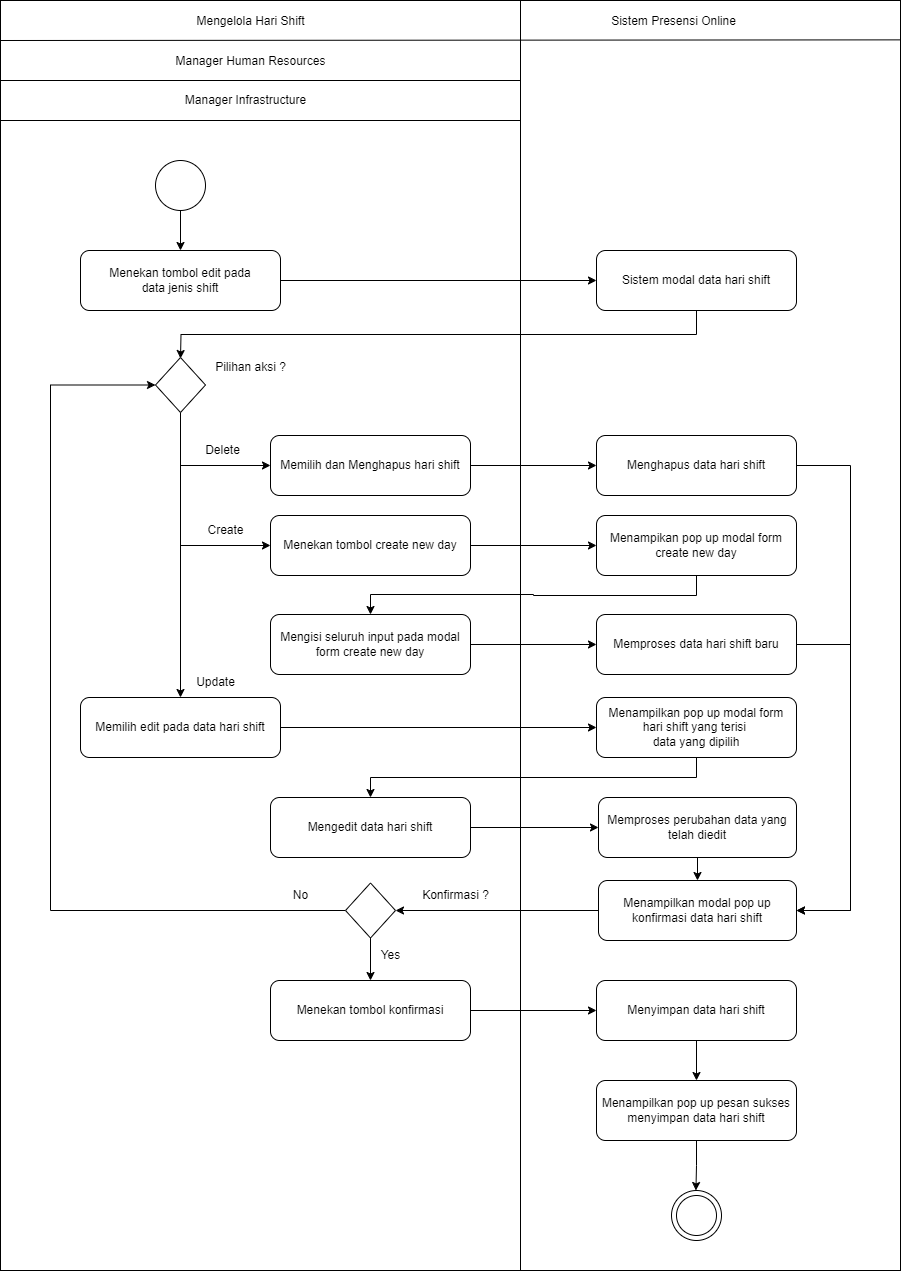
\includegraphics[width=15cm]{Gambar/bab2/activity-diagram-mengelola-data-hari-shift.png}
	\caption{\textit{Activity Diagram} Mengelola Hari \textit{Shift}}
	\label{fig:activity-diagram-mengelola-hari-shift}
\end{figure}
\FloatBarrier

\begin{figure}[H]
	\centering
	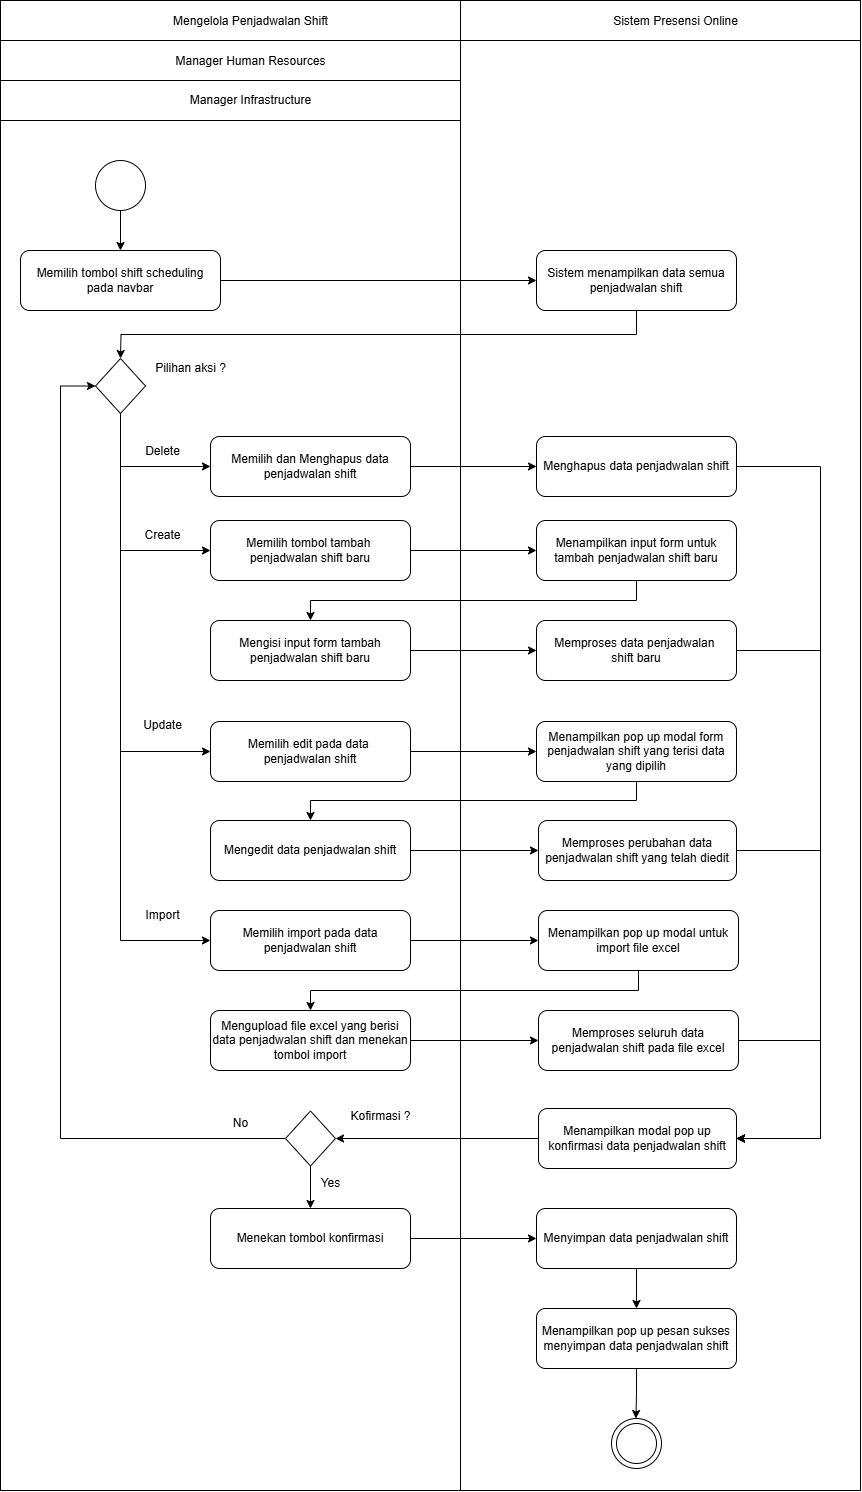
\includegraphics[width=13cm]{Gambar/bab2/activity-diagram-mengelola-penjadwalan-shift.png}
	\caption{\textit{Activity Diagram} Mengelola Penjadwalan \textit{Shift}}
	\label{fig:activity-diagram-mengelola-penjadwalan-shift}
\end{figure}
\FloatBarrier

\begin{figure}[H]
	\centering
	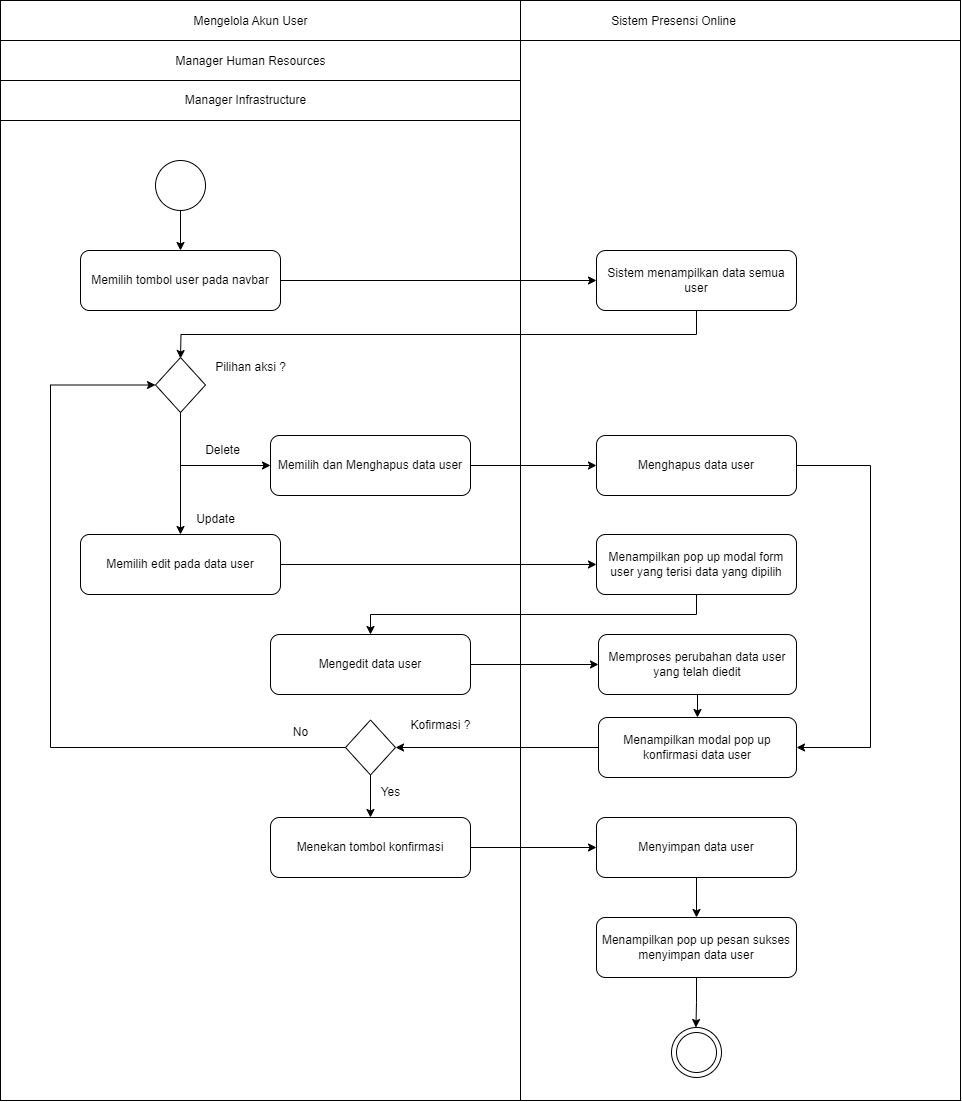
\includegraphics[width=15cm]{Gambar/bab2/activity-diagram-mengelola-data-user.png}
	\caption{\textit{Activity Diagram} Mengelola Akun \textit{User}}
	\label{fig:activity-diagram-mengelola-akun-user}
\end{figure}
\FloatBarrier

\begin{figure}[H]
	\centering
	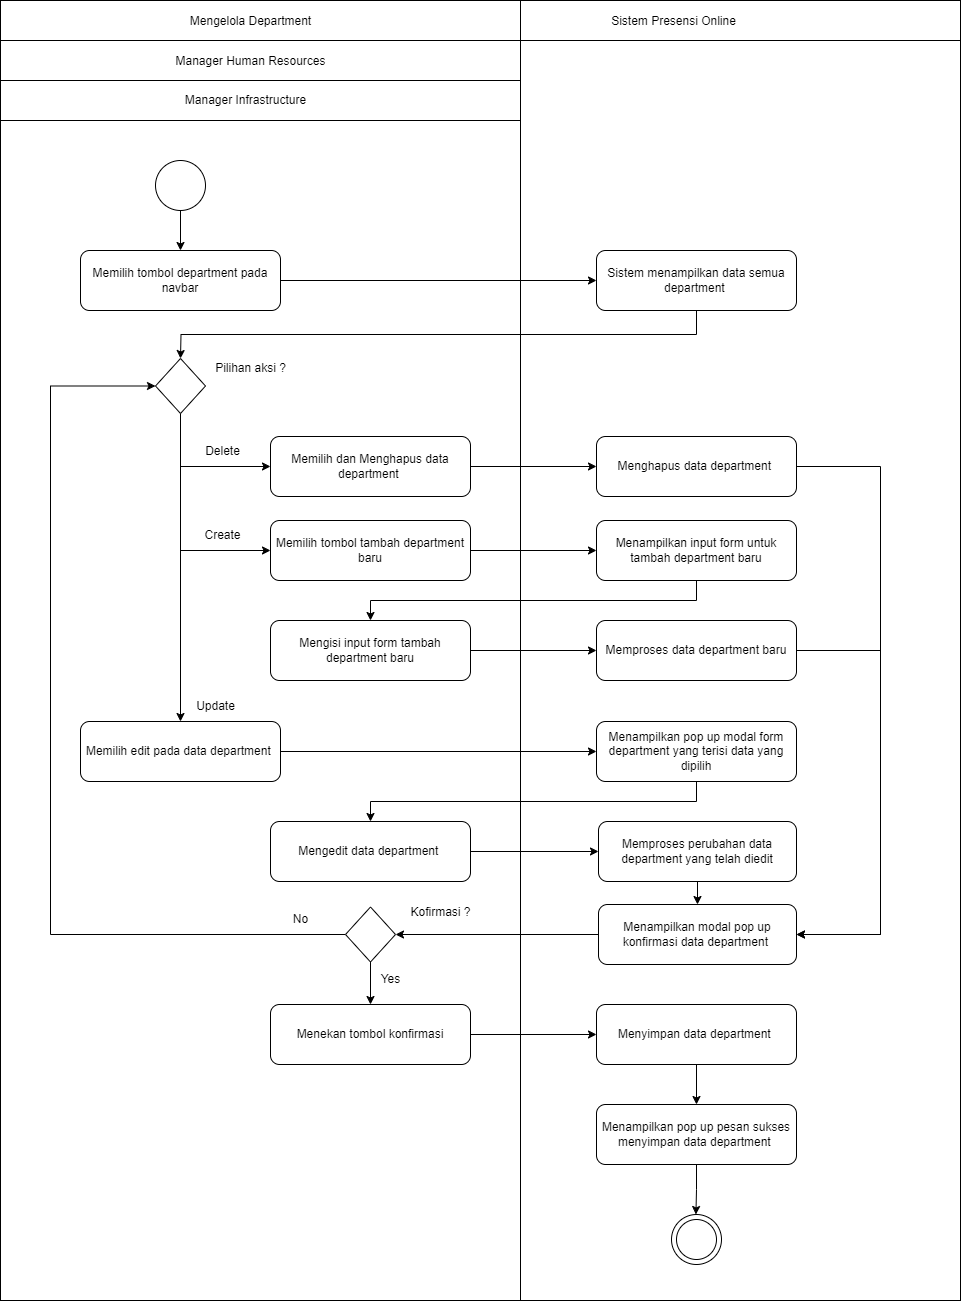
\includegraphics[width=15cm]{Gambar/bab2/activity-diagram-mengelola-data-department.png}
	\caption{\textit{Activity Diagram} Mengelola \textit{Department}}
	\label{fig:activity-diagram-mengelola-department}
\end{figure}
\FloatBarrier

\begin{figure}[H]
	\centering
	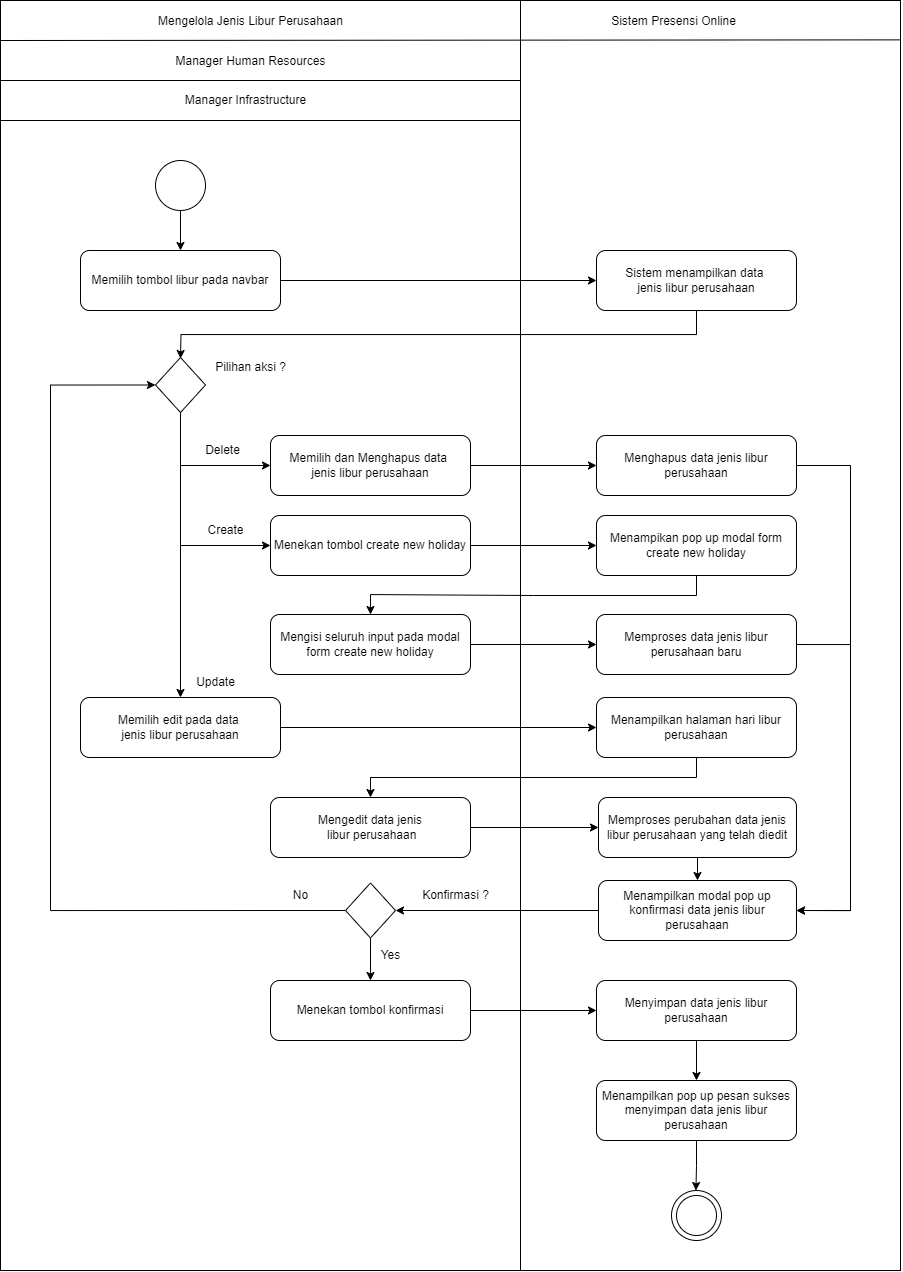
\includegraphics[width=13cm]{Gambar/bab2/activity-diagram-mengelola-data-jenis-libur-perusahaan.png}
	\caption{\textit{Activity Diagram} Mengelola Data Jenis Libur Perusahaan}
	\label{fig:activity-diagram-mengelola-data-jenis-libur-perusahaan}
\end{figure}
\FloatBarrier

\begin{figure}[H]
	\centering
	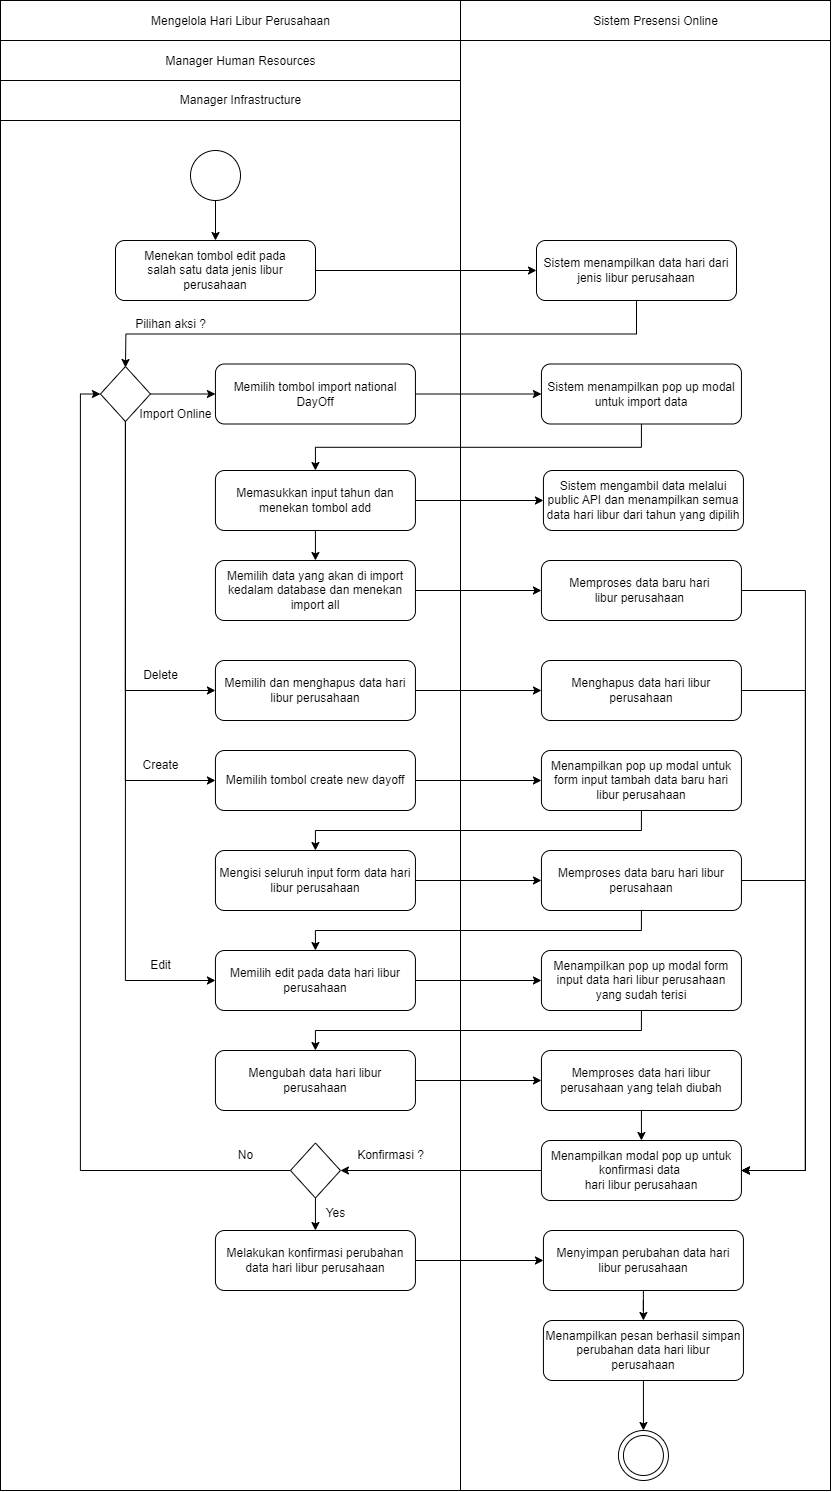
\includegraphics[width=13cm]{Gambar/bab2/activity-diagram-mengelola-data-hari-libur-perusahaan.png}
	\caption{\textit{Activity Diagram} Mengelola Data Hari Libur Perusahaan}
	\label{fig:activity-diagram-mengelola-data-hari-libur-perusahaan}
\end{figure}
\FloatBarrier

\begin{figure}[H]
	\centering
	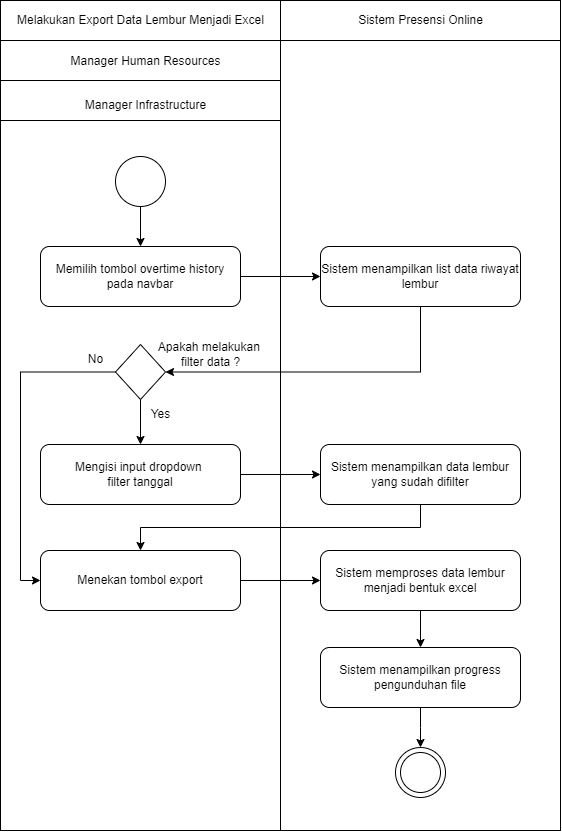
\includegraphics[width=15cm]{Gambar/bab2/activity-diagram-melakukan-export-data-lembur.png}
	\caption{\textit{Activity Diagram} Melakukan \textit{Export} Data Lembur ke \textit{Excel}}
	\label{fig:activity-diagram-melakukan-export-data-lembur-ke-excel}
\end{figure}
\FloatBarrier

\begin{figure}[H]
	\centering
	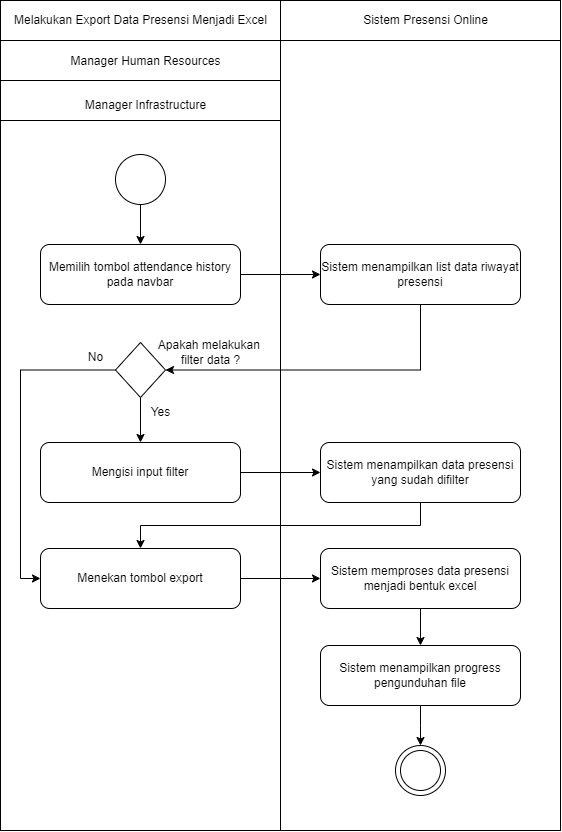
\includegraphics[width=15cm]{Gambar/bab2/activity-diagram-melakukan-export-data-presensi.png}
	\caption{\textit{Activity Diagram} Melakukan \textit{Export} Data Presensi ke \textit{Excel}}
	\label{fig:activity-diagram-melakukan-export-data-presensi-ke-excel}
\end{figure}
\FloatBarrier

\pagebreak

\nextappendix
\section*{Lampiran \theappendixletter: \textit{Sequence Diagram} Aplikasi Presensi \textit{Online} 
\label{sec:sequence-diagram-aplikasi-presensi-online}}
\addcontentsline{toc}{section}{Lampiran \theappendixletter: \textit{Sequence Diagram} Aplikasi Presensi \textit{Online}}
\begin{figure}[H]
	\centering
	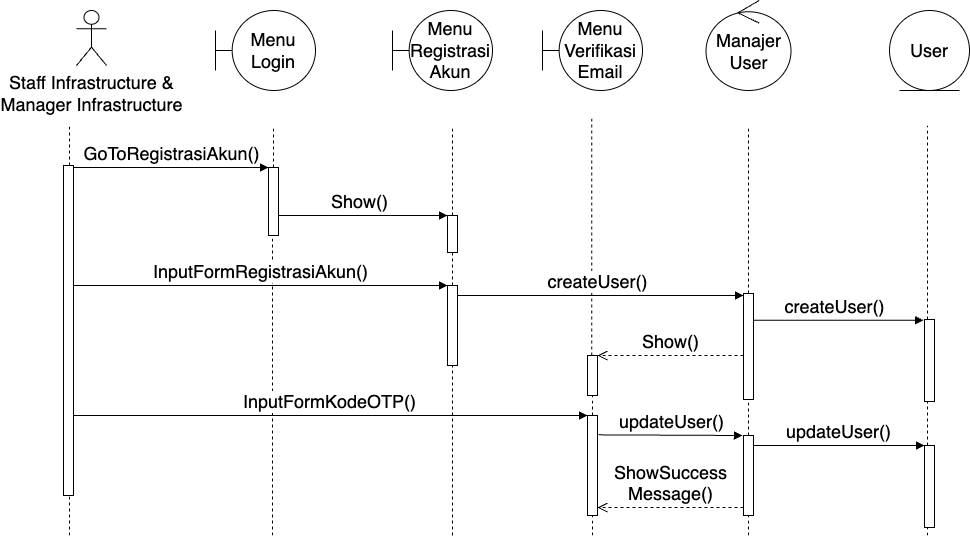
\includegraphics[width=15cm]{Gambar/bab2/sequence-diagram-registrasi-akun.png}
	\caption{\textit{Sequence Diagram} Registrasi Akun}
	\label{fig:sequence-diagram-registrasi-akun}
\end{figure}
\FloatBarrier

\begin{figure}[H]
	\centering
	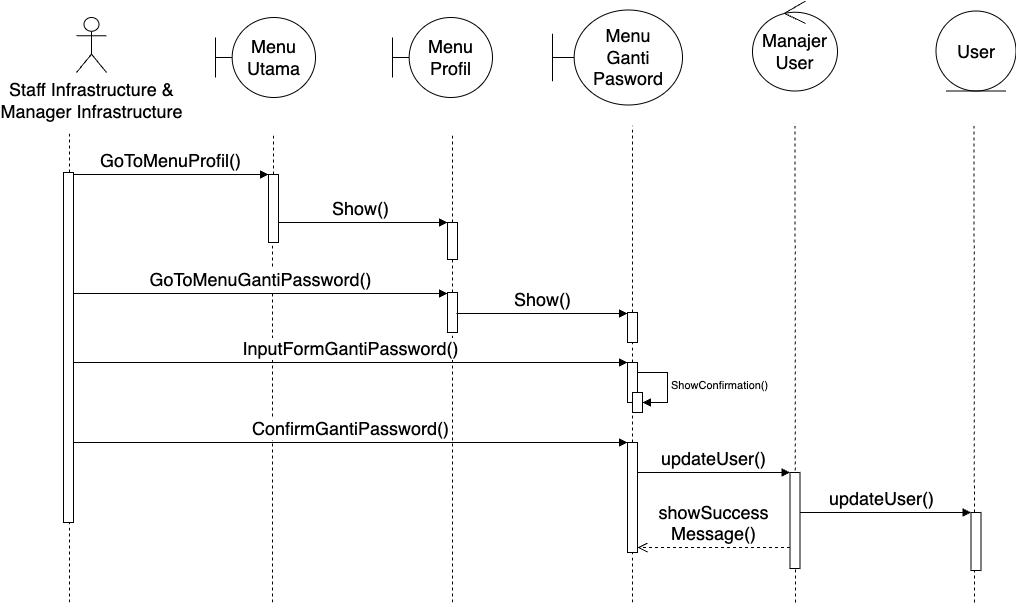
\includegraphics[width=15cm]{Gambar/bab2/sequence-diagram-ganti-password.png}
	\caption{\textit{Sequence Diagram} Ganti Password}
	\label{fig:sequence-diagram-ganti-password}
\end{figure}
\FloatBarrier

\begin{figure}[H]
	\centering
	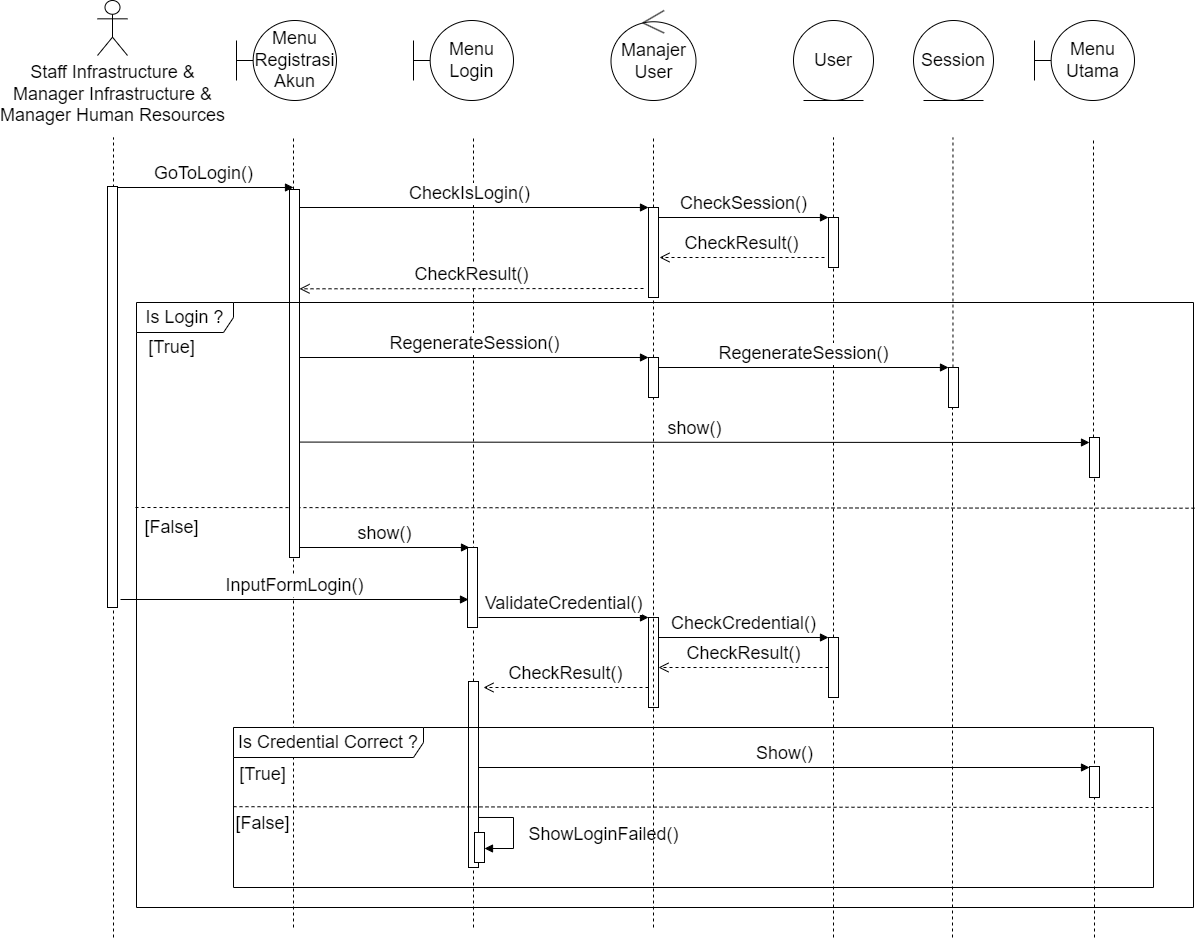
\includegraphics[width=17cm]{Gambar/bab2/sequence-diagram-login.png}
	\caption{\textit{Sequence Diagram Login}}
	\label{fig:sequence-diagram-login}
\end{figure}
\FloatBarrier

\begin{figure}[H]
	\centering
	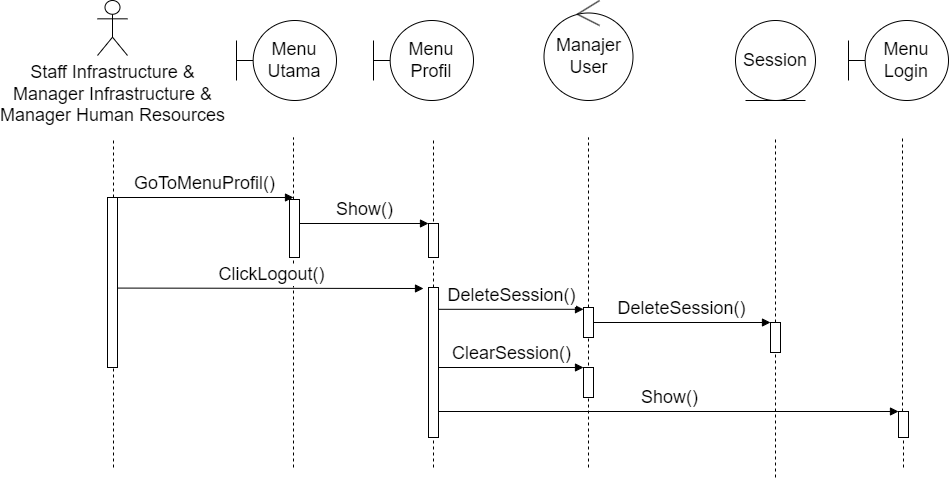
\includegraphics[width=17cm]{Gambar/bab2/sequence-diagram-logout.png}
	\caption{\textit{Sequence Diagram Logout}}
	\label{fig:sequence-diagram-logout}
\end{figure}
\FloatBarrier

\begin{figure}[H]
	\centering
	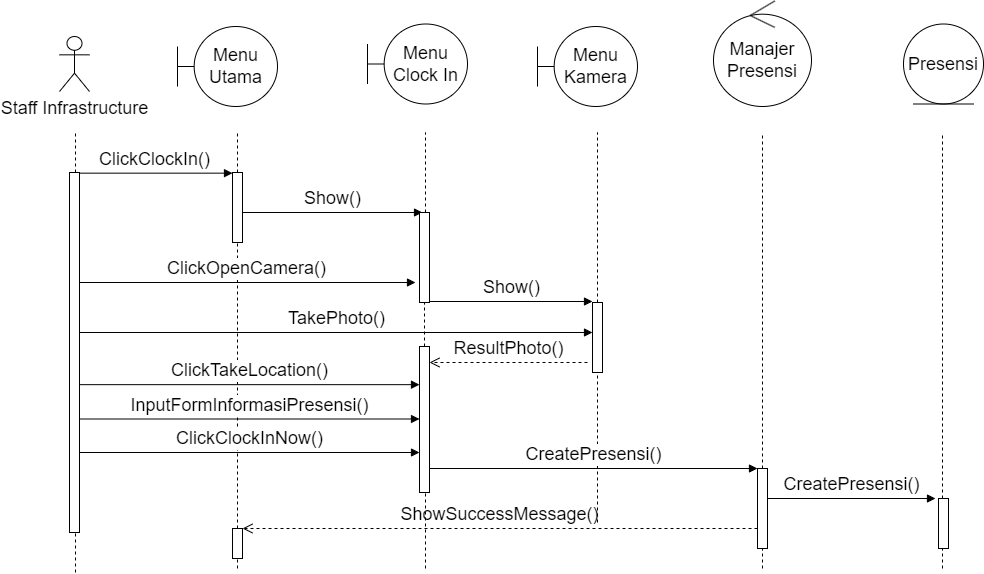
\includegraphics[width=17cm]{Gambar/bab2/sequence-diagram-clock-in.png}
	\caption{\textit{Sequence Diagram Clock In}}
	\label{fig:sequence-diagram-clock-in}
\end{figure}
\FloatBarrier

\begin{figure}[H]
	\centering
	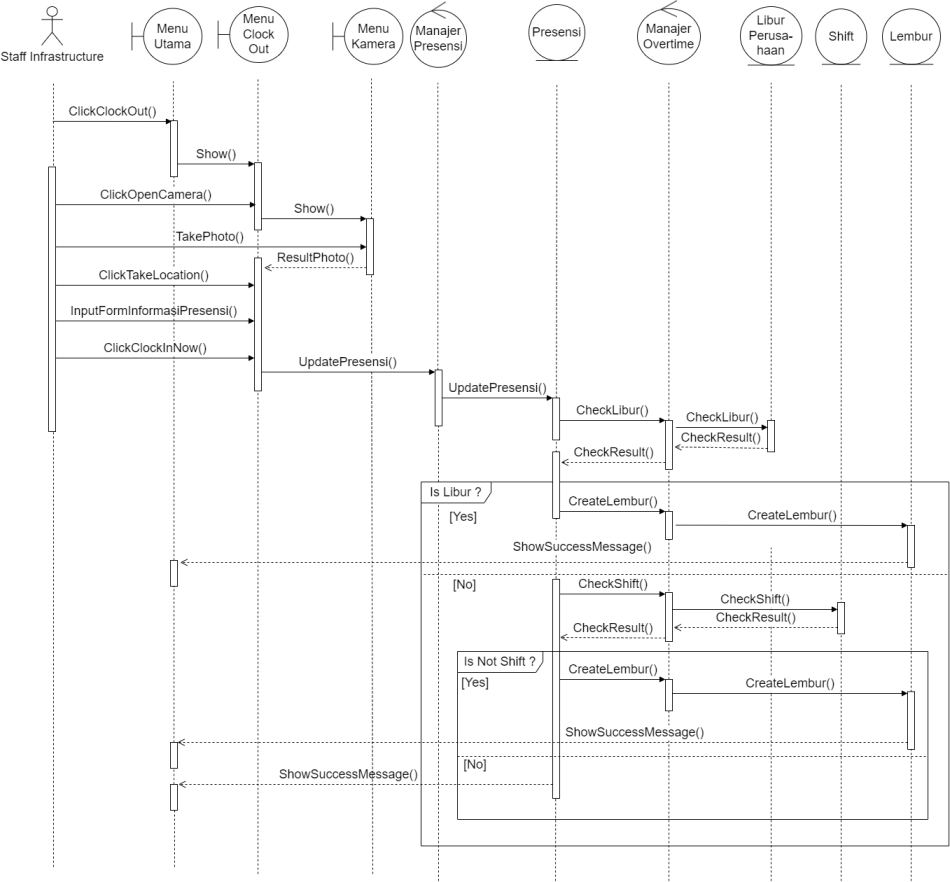
\includegraphics[width=18cm]{Gambar/bab2/sequence-diagram-clock-out.png}
	\caption{\textit{Sequence Diagram Clock Out}}
	\label{fig:sequence-diagram-clock-out}
\end{figure}
\FloatBarrier

\begin{figure}[H]
	\centering
	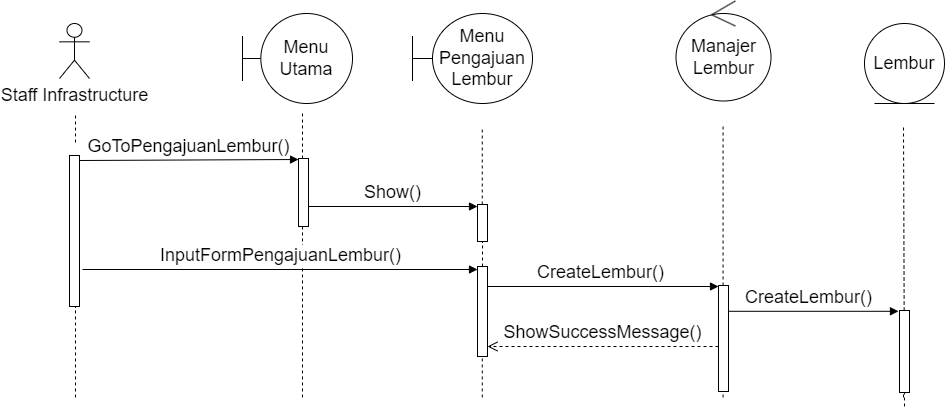
\includegraphics[width=17cm]{Gambar/bab2/sequence-diagram-melakukan-pengajuan-lembur.png}
	\caption{\textit{Sequence Diagram} Melakukan Pengajuan Lembur}
	\label{fig:sequence-diagram-melakukan-pengajuan-lembur}
\end{figure}
\FloatBarrier

\begin{figure}[H]
	\centering
	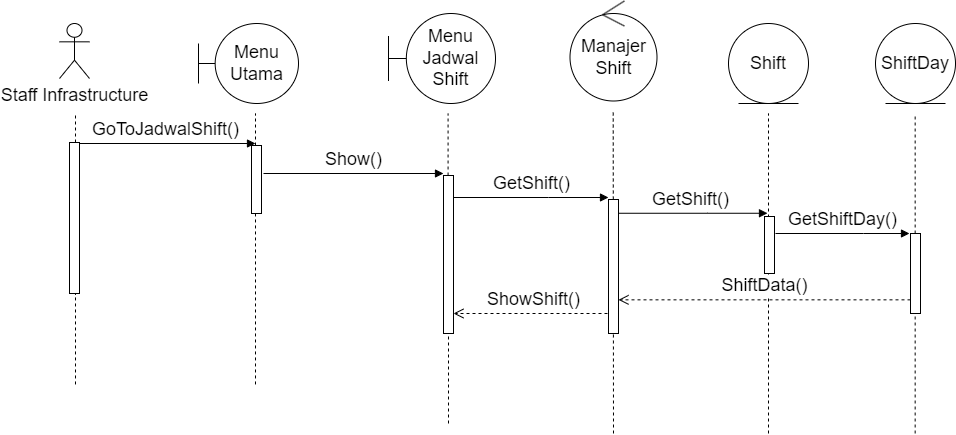
\includegraphics[width=17cm]{Gambar/bab2/sequence-diagram-melihat-jadwal-shift.png}
	\caption{\textit{Sequence Diagram} Melihat Jadwal \textit{Shift} Kerja}
	\label{fig:sequence-diagram-melihat-jadwal-shift-kerja}
\end{figure}
\FloatBarrier

\begin{figure}[H]
	\centering
	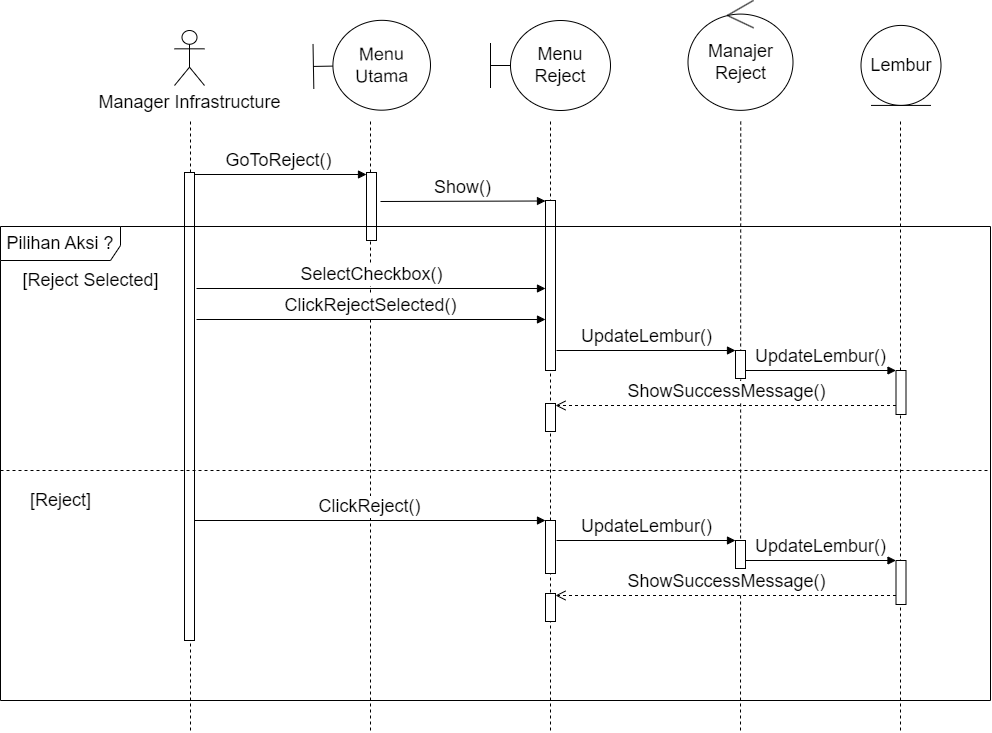
\includegraphics[width=17cm]{Gambar/bab2/sequence-diagram-melakukan-reject.png}
	\caption{\textit{Sequence Diagram} Melakukan \textit{Reject} pada Data Lembur}
	\label{fig:sequence-diagram-melakukan-reject-pada-data-lembur}
\end{figure}
\FloatBarrier

\begin{figure}[H]
	\centering
	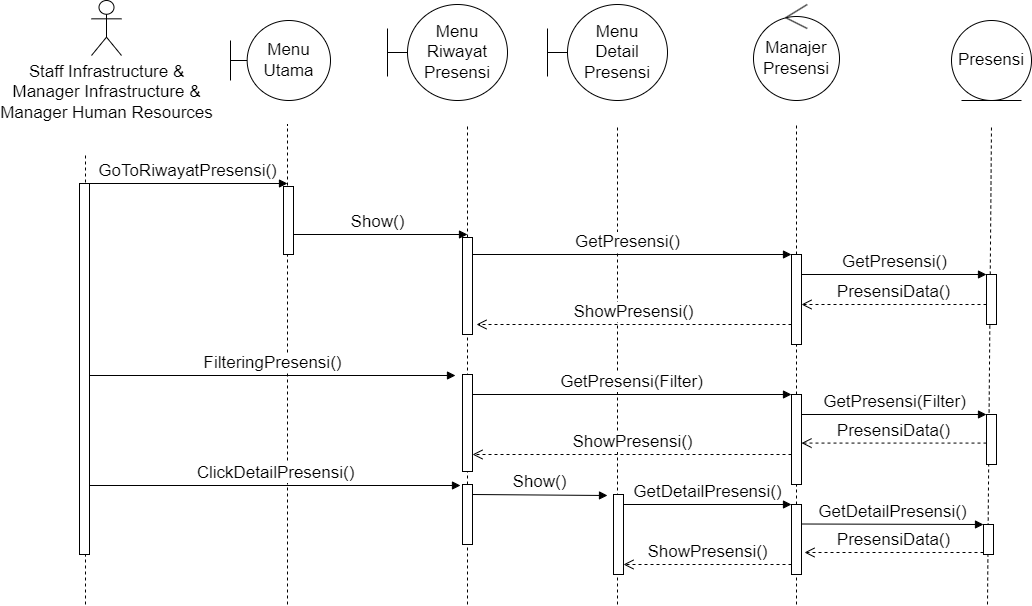
\includegraphics[width=17cm]{Gambar/bab2/sequence-diagram-melihat-riwayat-presensi.png}
	\caption{\textit{Sequence Diagram} Melihat Riwayat Presensi}
	\label{fig:sequence-diagram-melihat-riwayat-presensi}
\end{figure}
\FloatBarrier

\begin{figure}[H]
	\centering
	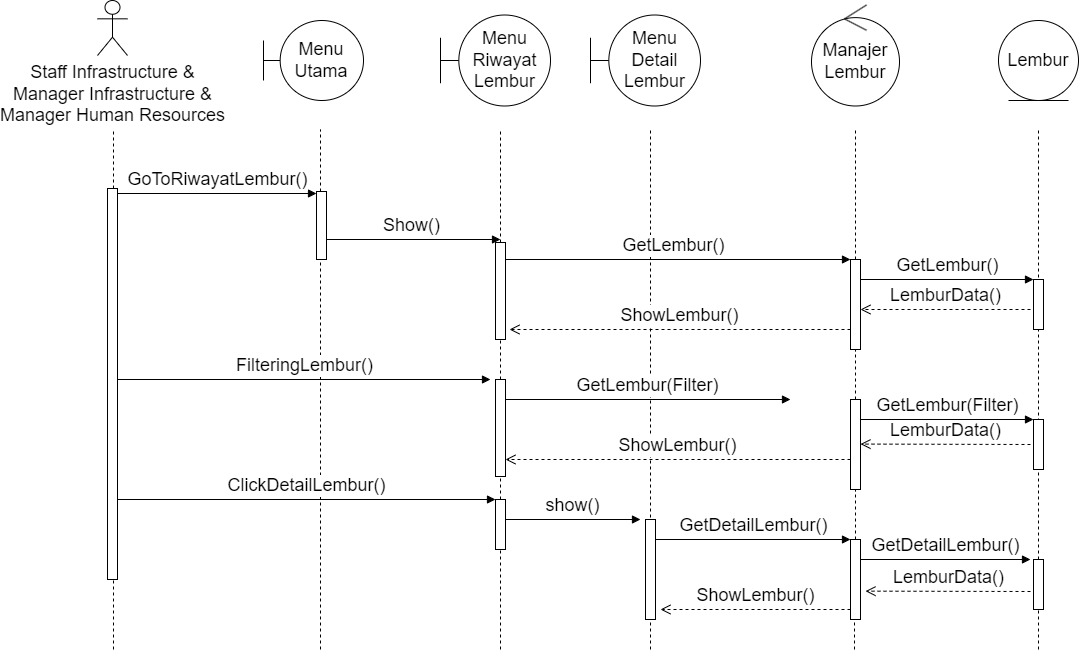
\includegraphics[width=17cm]{Gambar/bab2/sequence-diagram-melihat-riwayat-lembur.png}
	\caption{\textit{Sequence Diagram} Melihat Riwayat Lembur}
	\label{fig:sequence-diagram-melihat-riwayat-lembur}
\end{figure}
\FloatBarrier

\begin{figure}[H]
	\centering
	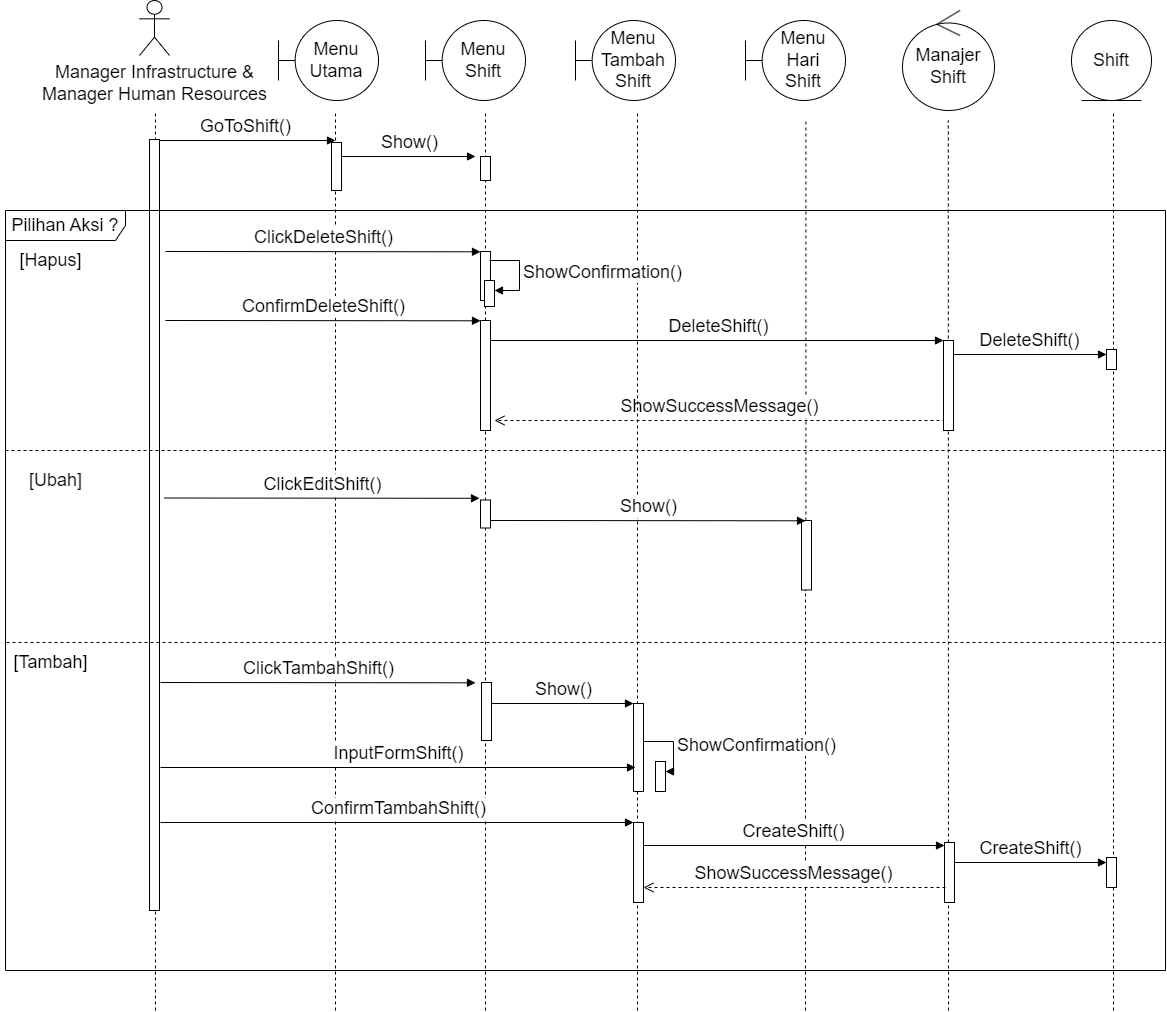
\includegraphics[width=18cm]{Gambar/bab2/sequence-diagram-mengelola-data-jenis-shift.png}
	\caption{\textit{Sequence Diagram} Mengelola Jenis \textit{Shift}}
	\label{fig:sequence-diagram-mengelola-jenis-shift}
\end{figure}
\FloatBarrier

\begin{figure}[H]
	\centering
	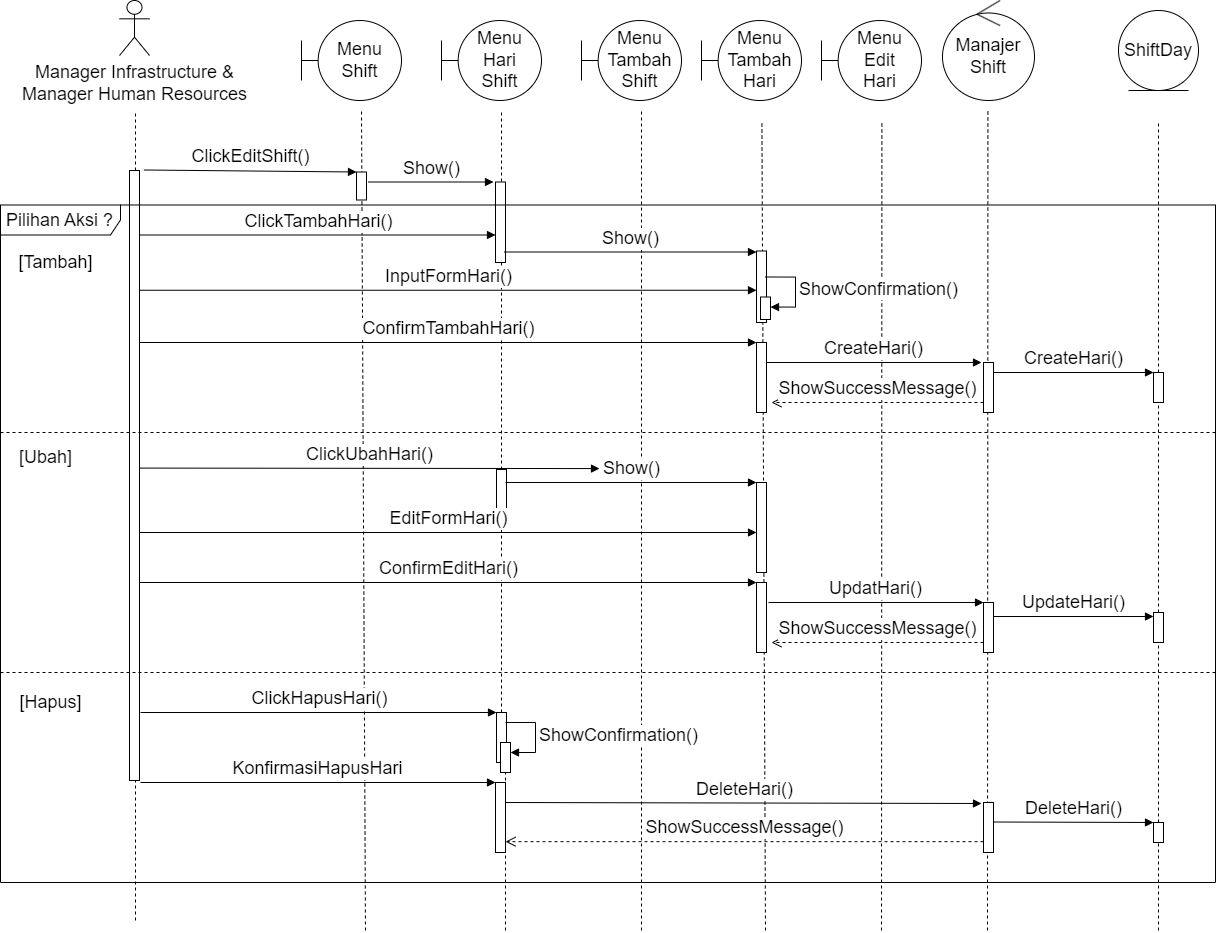
\includegraphics[width=18cm]{Gambar/bab2/sequence-diagram-mengelola-data-hari-shift.png}
	\caption{\textit{Sequence Diagram} Mengelola Hari \textit{Shift}}
	\label{fig:sequence-diagram-mengelola-hari-shift}
\end{figure}
\FloatBarrier

\begin{figure}[H]
	\centering
	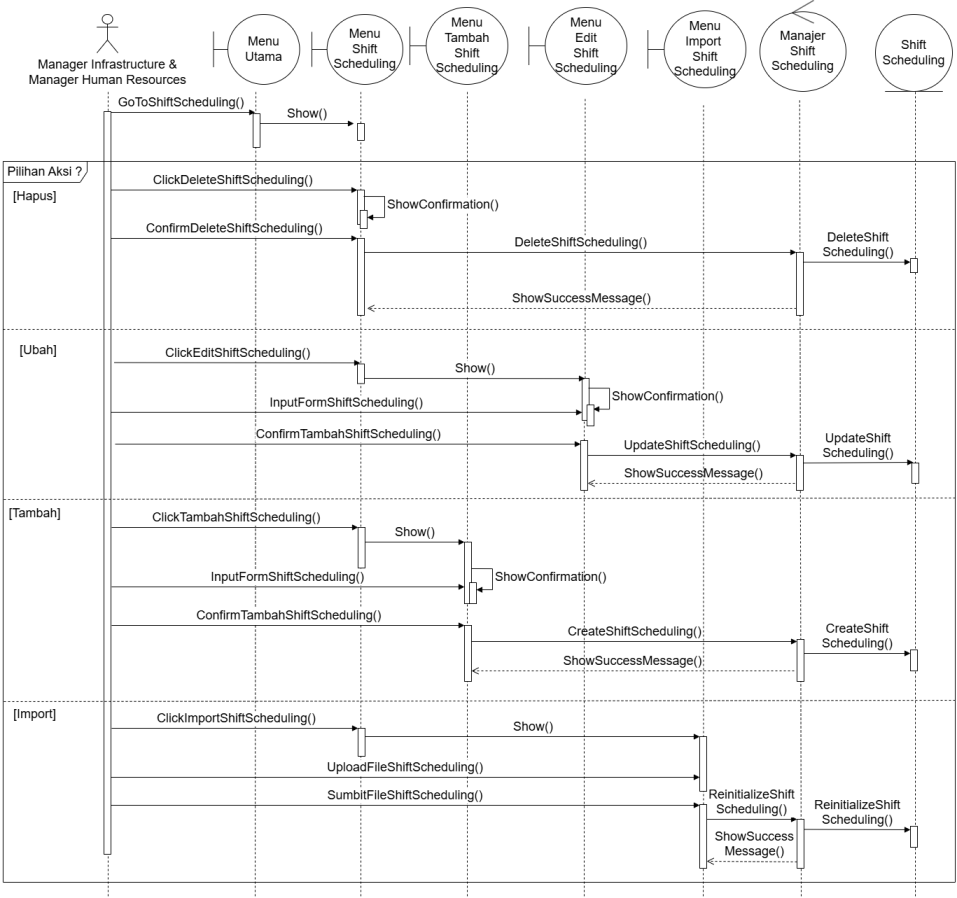
\includegraphics[width=18cm]{Gambar/bab2/sequence-diagram-mengelola-data-penjadwalan-shift.png}
	\caption{\textit{Sequence Diagram} Mengelola Penjadwalan \textit{Shift}}
	\label{fig:sequence-diagram-mengelola-penjadwalan-shift}
\end{figure}
\FloatBarrier

\begin{figure}[H]
	\centering
	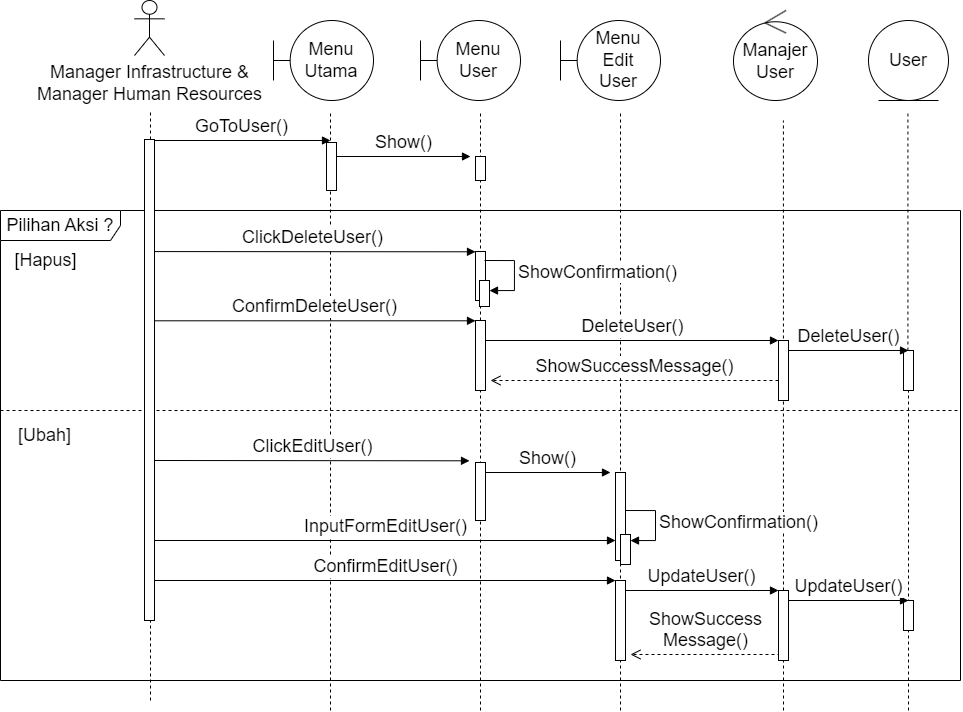
\includegraphics[width=15cm]{Gambar/bab2/sequence-diagram-mengelola-akun-user.png}
	\caption{\textit{Sequence Diagram} Mengelola Akun \textit{User}}
	\label{fig:sequence-diagram-mengelola-akun-user}
\end{figure}
\FloatBarrier

\begin{figure}[H]
	\centering
	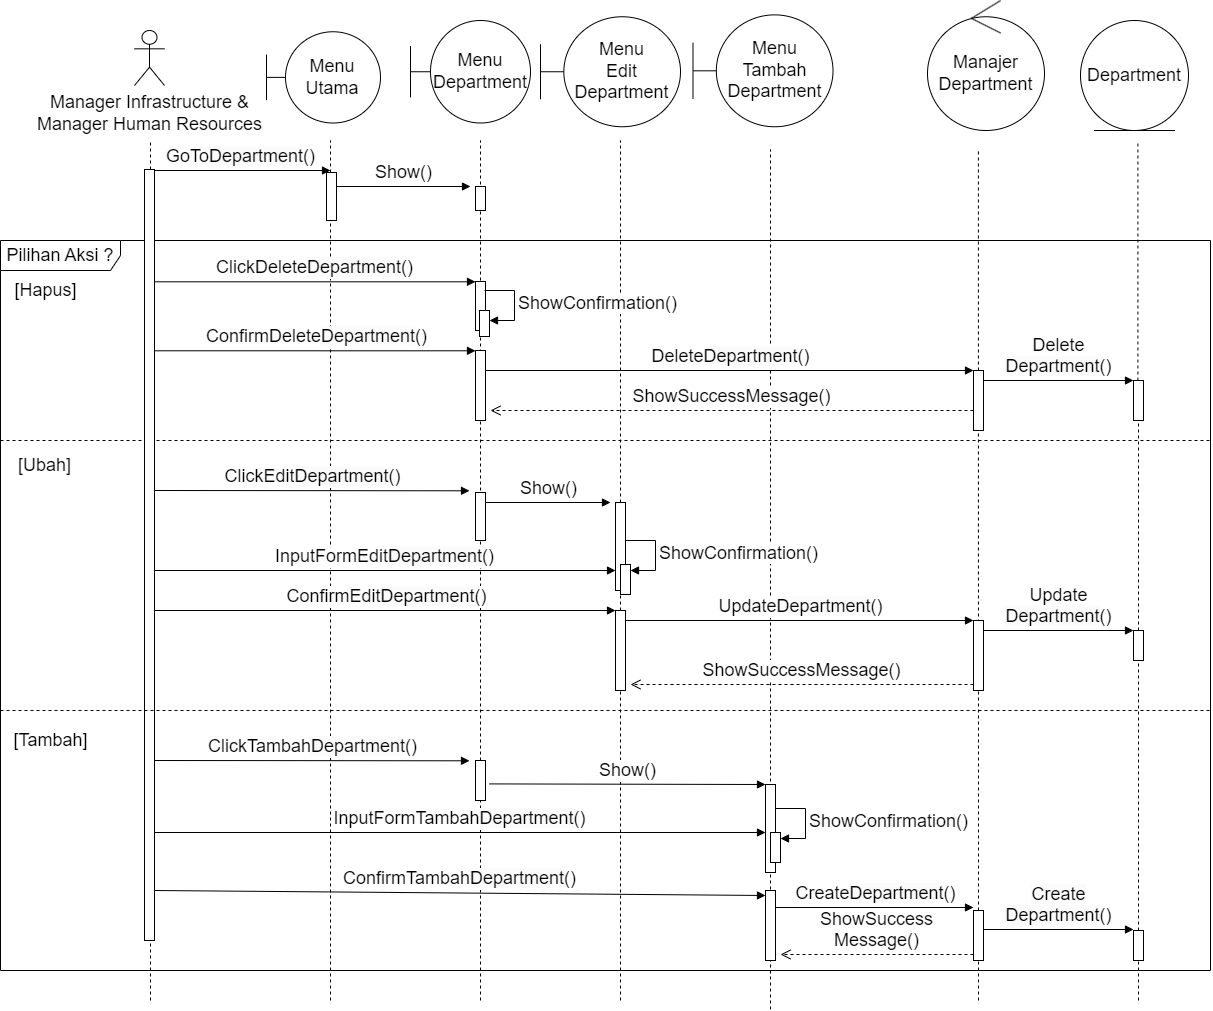
\includegraphics[width=15cm]{Gambar/bab2/sequence-diagram-mengelola-department.png}
	\caption{\textit{Sequence Diagram} Mengelola \textit{Department}}
	\label{fig:sequence-diagram-mengelola-department}
\end{figure}
\FloatBarrier

\begin{figure}[H]
	\centering
	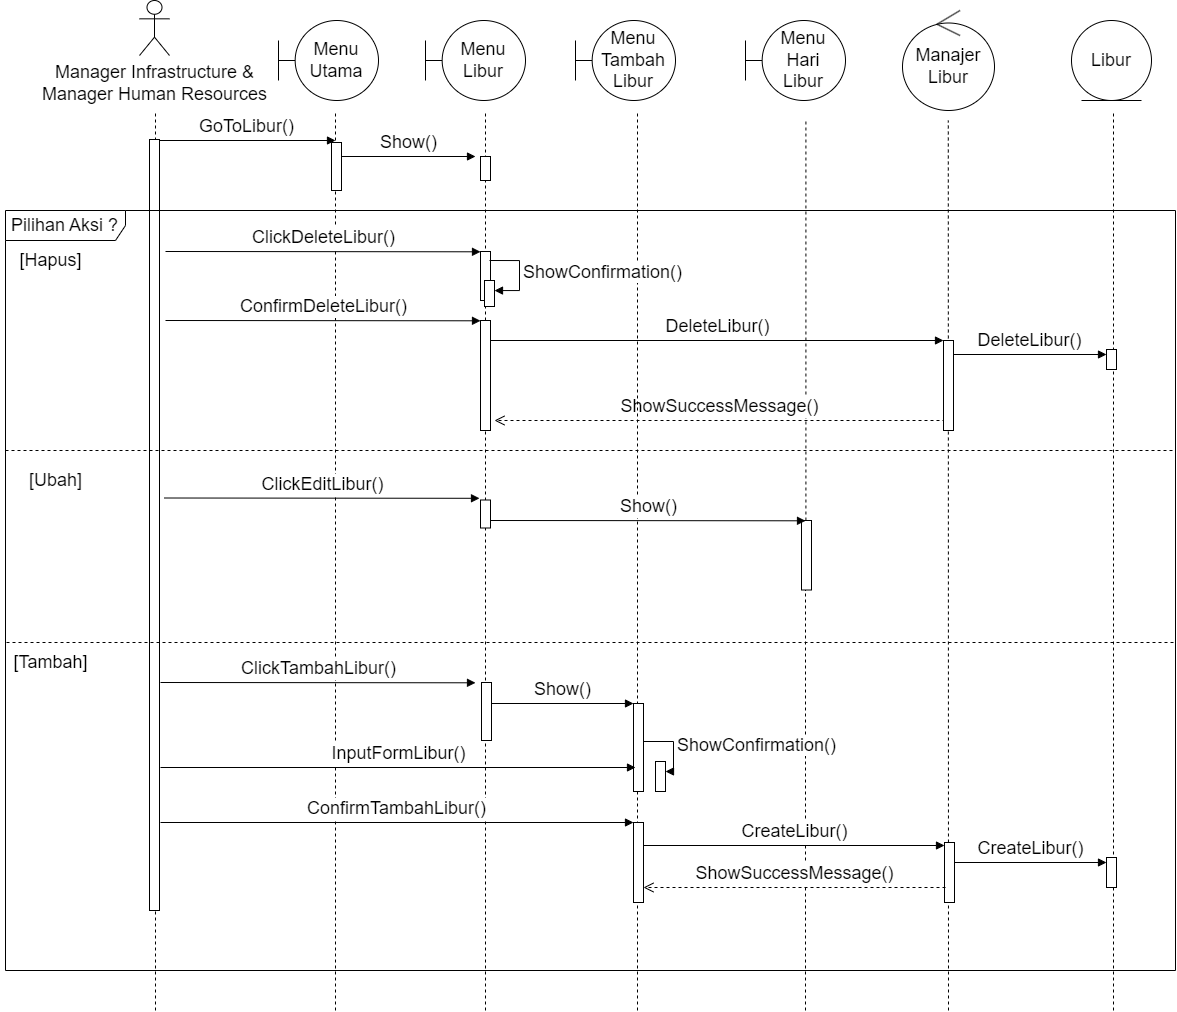
\includegraphics[width=15cm]{Gambar/bab2/sequence-diagram-mengelola-data-jenis-libur.png}
	\caption{\textit{Sequence Diagram} Mengelola Data Jenis Libur Perusahaan}
	\label{fig:sequence-diagram-mengelola-data-jenis-libur-perusahaan}
\end{figure}
\FloatBarrier

\begin{figure}[H]
	\centering
	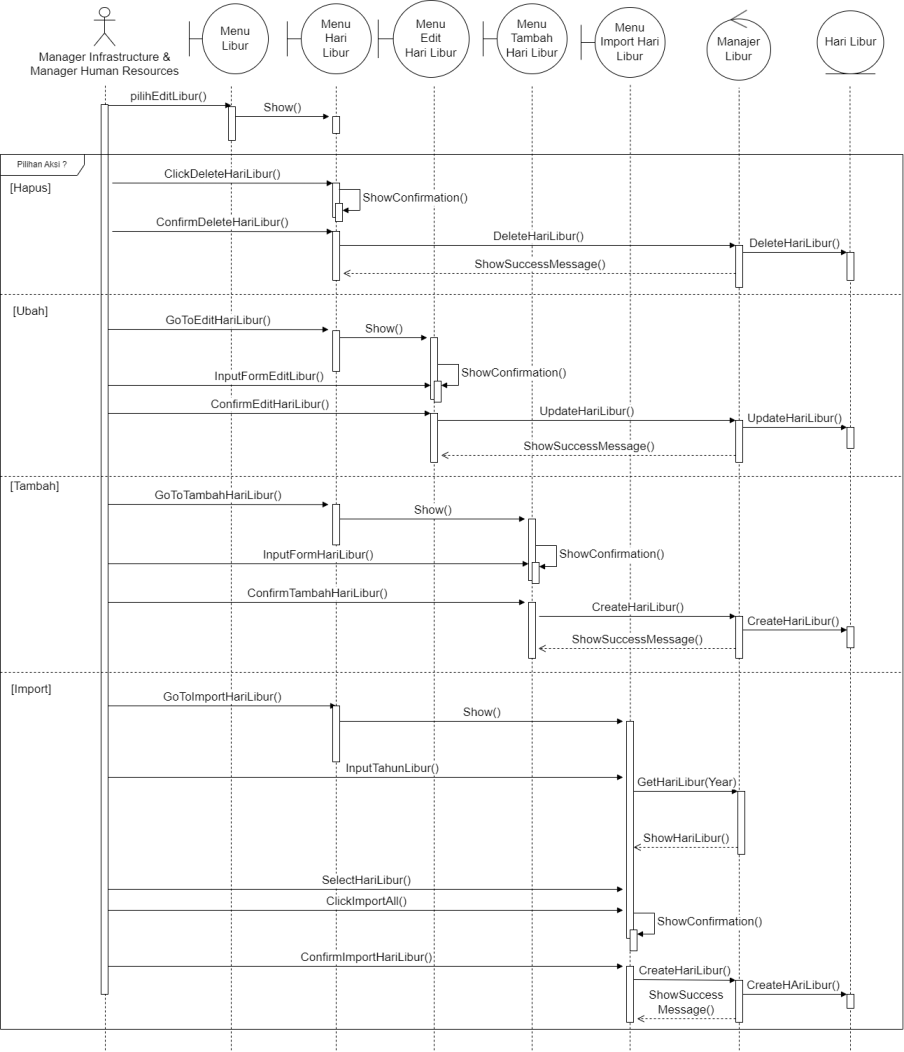
\includegraphics[width=15cm]{Gambar/bab2/sequence-diagram-mengelola-data-hari-libur.png}
	\caption{\textit{Sequence Diagram} Mengelola Data Hari Libur Perusahaan}
	\label{fig:sequence-diagram-mengelola-data-hari-libur-perusahaan}
\end{figure}
\FloatBarrier

\begin{figure}[H]
	\centering
	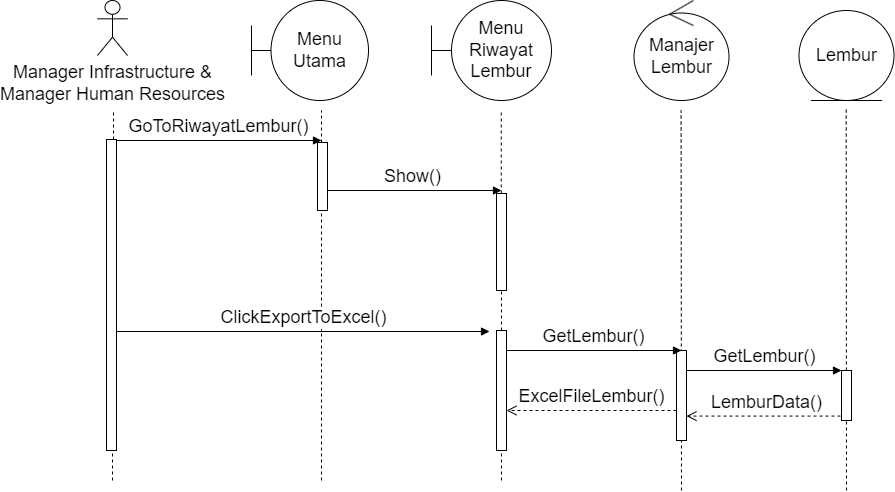
\includegraphics[width=15cm]{Gambar/bab2/sequence-diagram-melakukan-export-data-lembur-ke-excel.png}
	\caption{\textit{Sequence Diagram} melakukan \textit{Export} Data Lembur ke \textit{Excel}}
	\label{fig:sequence-diagram-melakukan-export-data-lembur-ke-excel}
\end{figure}
\FloatBarrier

\begin{figure}[H]
	\centering
	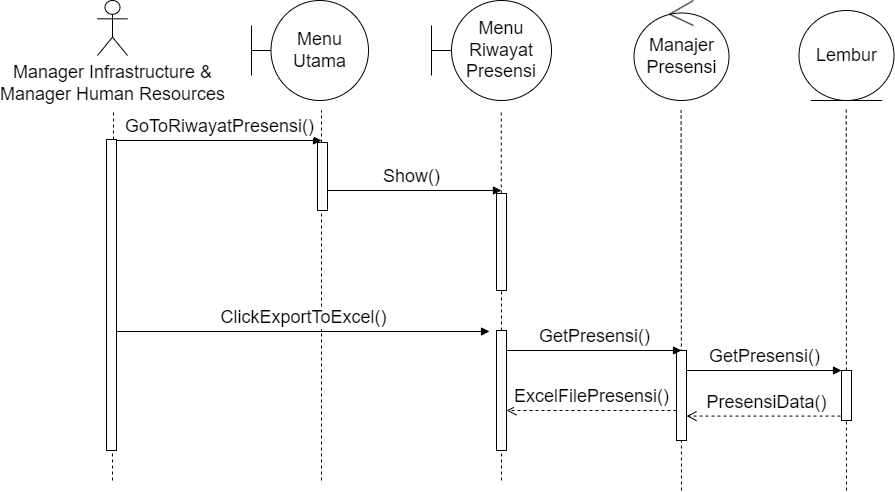
\includegraphics[width=15cm]{Gambar/bab2/sequence-diagram-melakukan-export-data-presensi-ke-excel.png}
	\caption{\textit{Sequence Diagram} melakukan \textit{Export} Data Presensi ke \textit{Excel}}
	\label{fig:sequence-diagram-melakukan-export-data-presensi-ke-excel}
\end{figure}
\FloatBarrier
\pagebreak


\begin{landscape}
\nextappendix
\section*{Lampiran \theappendixletter: \textit{Class Diagram} Aplikasi Presensi \textit{Online}}
\label{sec:class-diagram-aplikasi-presensi-online}
\addcontentsline{toc}{section}{Lampiran \theappendixletter: \textit{Class Diagram} Aplikasi Presensi \textit{Online}}
\begin{figure}[H]
	\centering
	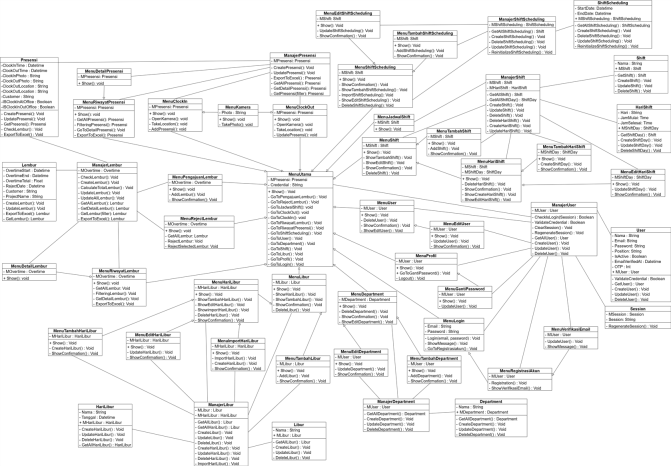
\includegraphics[width=21cm]{Gambar/bab2/class-diagram.png}
	\caption{\textit{Class Diagram} Aplikasi Presensi \textit{Online}}
	\label{fig:class-diagram-aplikasi-presensi-online}
\end{figure}
\end{landscape}

\nextappendix
\section*{Lampiran \theappendixletter: \textit{Conceptual Data Modeling}}
\label{sec:conceptual-database-design}
\addcontentsline{toc}{section}{Lampiran \theappendixletter: \textit{Conceptual Data Modeling}}
\begin{figure}[H]
	\centering
	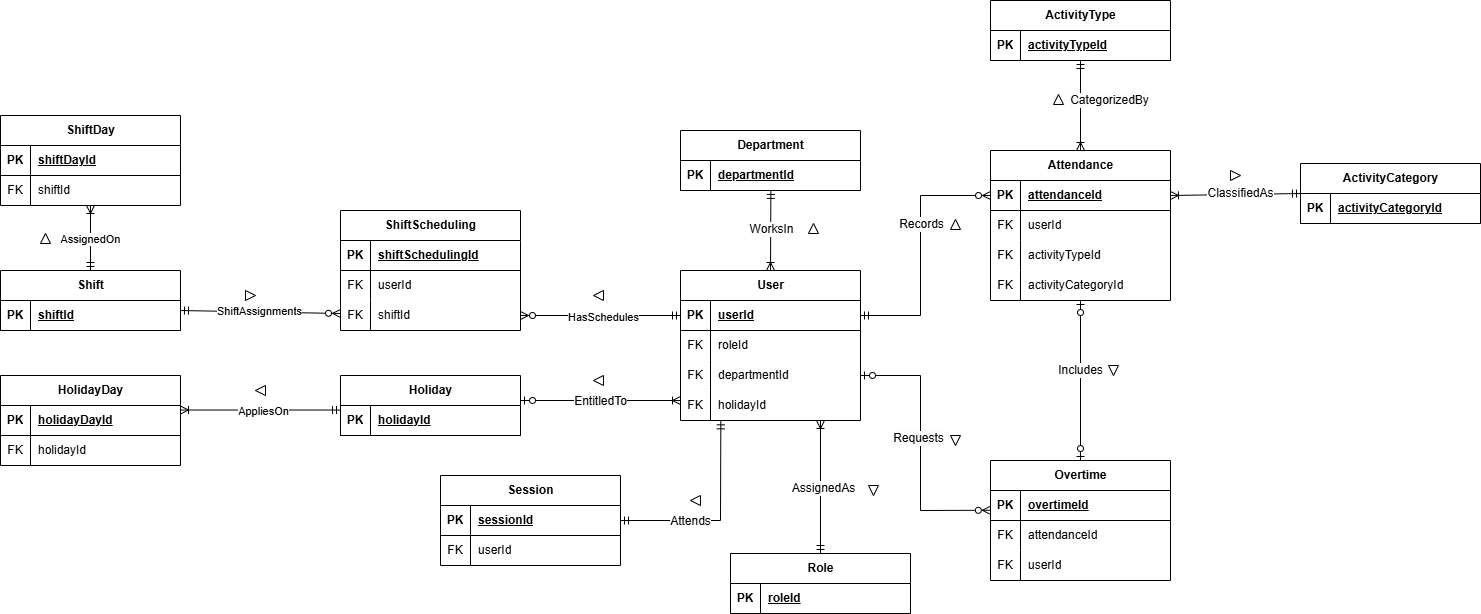
\includegraphics[width=17cm]{Gambar/bab2/conceptual-database-design.png}
	\caption{\textit{Conceptual Data Modeling}}
	\label{fig:conceptual-database-design}
\end{figure}

\nextappendix
\section*{Lampiran \theappendixletter: \textit{Logical Data Modeling}}
\label{sec:logical-database-design}
\addcontentsline{toc}{section}{Lampiran \theappendixletter: \textit{Logical Data Modeling}}
\begin{figure}[H]
	\centering
	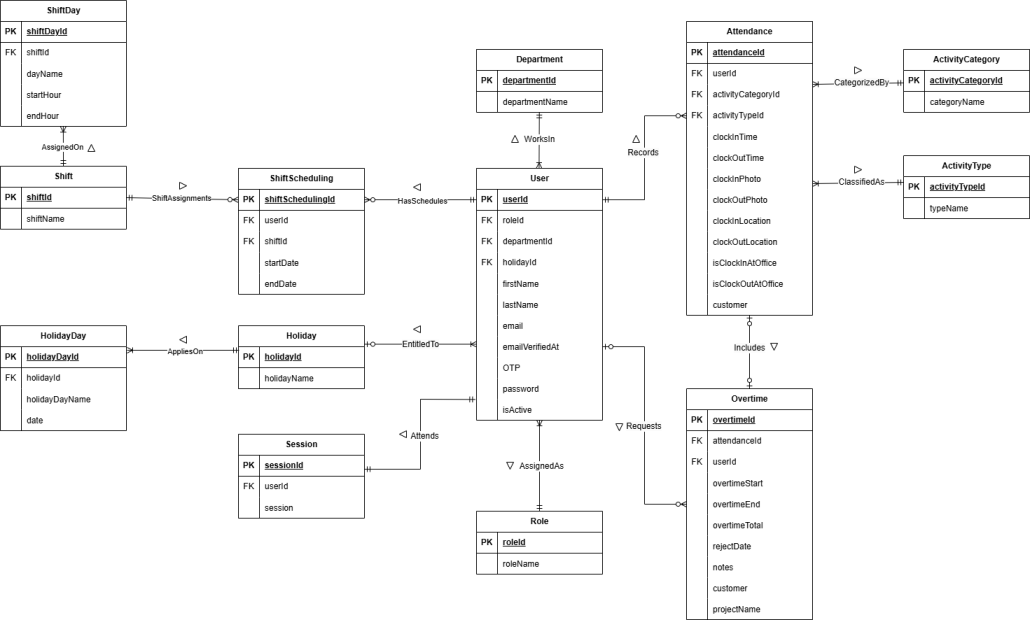
\includegraphics[width=17cm]{Gambar/bab2/logical-database-design.png}
	\caption{\textit{Logical Data Modeling}}
	\label{fig:logical-database-design}
\end{figure}


\begin{landscape}
\nextappendix
\section*{Lampiran \theappendixletter: \textit{Table Specification}
\label{sec:table-specification}}
\addcontentsline{toc}{section}{Lampiran \theappendixletter: \textit{Table Specification}}
\begin{longtable}{ |p{3cm}|p{3cm}|p{4cm}|p{3cm}|p{2cm}|p{2cm}|p{2cm}|}
\caption{\textit{Table Specification}}\label{tab:table-specification} 
\\
\hline
\textbf{\textit{Entity}}
&\textbf{\textit{Attributes}}
&\textbf{\textit{Description}}
&\textbf{\textit{Data Types}}
&\textbf{\textit{Nullvalue}}
&\textbf{\textit{Multivalue}}
&\textbf{\textit{Composite}}
\\ 
\hline

\multirow{9}{*}{\textit{User}}
&userId
&Primary key
&INT
&No
&No
&No
\\
\cline{2-7}
&roleId
&Foreign key \textit{entity} Role
&INT
&No
&No
&No
\\ 
\cline{2-7}
&departmentId
&Foreign key \textit{entity} Department
&INT
&No
&No
&No
\\ 
\cline{2-7}
&holidayId
&Foreign key \textit{entity} Holiday
&INT
&Yes
&No
&No
\\ 
\cline{2-7}
&emailVerifiedAt
&Waktu verifikasi \textit{email}
&Datetime
&yes
&No
&No
\\ 
\cline{2-7}
&firstName
&Nama depan user
&VARCHAR(50)
&No
&No
&No
\\ 
\cline{2-7}
&lastName
&Nama belakang user
&VARCHAR(50)
&No
&No
&No
\\ 
\cline{2-7}
&email
&Email user yang unik
&VARCHAR(50)
&No
&No
&No
\\ 
\cline{2-7}
&password
&Password user dalam bentuk hash.
&VARCHAR(50)
&No
&No
&No
\\ 
\hline

\multirow{2}{*}{}
&isActive
&Status apakah user aktif atau tidak.
&BOOLEAN
&No
&No
&No
\\ 
\cline{2-7}
&OTP
&6 digit kode OTP untuk verifikasi \textit{email}
&INT
&Yes
&No
&No
\\ 
\hline

\multirow{3}{*}{\textit{Session}}
&sessionId
&Primary key
&INT
&No
&No
&No
\\
\cline{2-7}
&userId
&Foreign key \textit{entity} User
&INT
&No
&No
&No
\\ 
\cline{2-7}
&session
&Pengenal unik yang mendefinisikan sesi pengguna saat login
&String
&No
&No
&No
\\ 
\hline

\multirow{4}{*}{\textit{Attendance}}
&attendanceId
&Primary key
&INT
&No
&No
&No
\\
\cline{2-7}
&userId
&Foreign key \textit{entity} User
&INT
&No
&No
&No
\\ 
\cline{2-7}
&activityTypeId
&Foreign key \textit{entity} ActivityType
&INT
&No
&No
&No
\\ 
\cline{2-7}
&activityCategoryId
&Foreign key \textit{entity} ActivityCategory
&INT
&No
&No
&No
\\ 
\hline

\multirow{8}{*}{}
&clockInTime
&Waktu user melakukan \textit{clock in}
&DATETIME
&No
&No
&No
\\ 
\cline{2-7}
&clockOutTime
&Waktu user melakukan \textit{clock out}
&DATETIME
&Yes
&No
&No
\\ 
\cline{2-7}
&clockInPhoto 
&\textit{Path} ke foto saat \textit{clock in}
&VARCHAR(255)
&No
&No
&No
\\ 
\cline{2-7}
&clockOutPhoto
&\textit{Path} ke foto saat \textit{clock out}
&VARCHAR(255)
&Yes
&No
&No
\\ 
\cline{2-7}
&clockInLocation
&Lokasi saat \textit{clock in}
&VARCHAR(255)
&No
&No
&No
\\ 
\cline{2-7}
&clockOutLocation
&Lokasi saat \textit{clock out}
&VARCHAR(255)
&Yes
&No
&No
\\ 
\cline{2-7}
&customer
&Nama customer saat presensi
&String
&Yes
&No
&No
\\ 
\cline{2-7}
&isClockInAtOffice
&Informasi terkait presensi masuk dilakukan diluar atau didalam radius kantor
&Boolean
&No
&No
&No
\\ 
\hline

\multirow{1}{*}{}
&isClockOutAtOffice
&Informasi terkait presensi keluar dilakukan diluar atau didalam radius kantor
&Boolean
&No
&No
&No
\\ 
\hline

\multirow{2}{*}{\textit{Department}}
&departmentId
&Primary key
&INT
&No
&No
&No
\\
\cline{2-7}
&departmentName
&Nama departemen atau divisi dari user
&VARCHAR(50)
&No
&No
&No
\\ 
\hline

\multirow{2}{*}{\textit{Role}}
&roleId
&Primary key
&INT
&No
&No
&No
\\
\cline{2-7}
&roleName
&Nama role atau jabatan dari user
&VARCHAR(50)
&No
&No
&No
\\ 
\hline

\multirow{2}{*}{\textit{Shift}}
&shiftId
&Primary key
&INT
&No
&No
&No
\\
\cline{2-7}
&shiftName
&Nama shift kerja
&VARCHAR(50)
&No
&No
&No
\\ 
\hline

\multirow{3}{*}{\textit{ShiftDay}}
&shiftDayId
&Primary key
&INT
&No
&No
&No
\\
\cline{2-7}
&shiftId
&Foreign key \textit{entity} Shift
&INT
&No
&No
&No
\\
\cline{2-7}
&dayName
&Nama hari dari setiap \textit{shift} kerja
&VARCHAR(20)
&No
&No
&No
\\
\hline

\multirow{2}{*}{}
&startHour
&Waktu mulai \textit{shift} kerja
&TIME
&No
&No
&No
\\
\cline{2-7}
&endHour
&Waktu selesai \textit{shift} kerja
&TIME
&No
&No
&No
\\ 
\hline

\multirow{2}{*}{\textit{Holiday}}
&Holiday
&Primary key
&INT
&No
&No
&No
\\
\cline{2-7}
&holidayName
&Nama jenis libur
&VARCHAR(50)
&No
&No
&No
\\ 
\hline

\multirow{4}{*}{\textit{HolidayDay}}
&holidayDayId
&Primary key
&INT
&No
&No
&No
\\
\cline{2-7}
&holidayId
&Foreign key \textit{entity} Holiday
&INT
&No
&No
&No
\\
\cline{2-7}
&date
&Tanggal hari libur perusahaan
&DATE
&No
&No
&No
\\
\cline{2-7}
&holidayName
&Nama hari libur perusahaan
&VARCHAR(50)
&No
&No
&No
\\ 
\hline

\multirow{3}{*}{\textit{Overtime}}
&overtimeId
&Primary key
&INT
&No
&No
&No
\\
\cline{2-7}
&attendanceId
&Foreign key \textit{entity} Attendance
&INT
&Yes
&No
&No
\\ 
\cline{2-7}
&userId
&Foreign key \textit{entity} User
&INT
&Yes
&No
&No
\\ 
\hline

\multirow{7}{*}{}
&overtimeStart 
&Waktu mulai lembur
&DATETIME
&No
&No
&No
\\ 
\cline{2-7}
&overtimeEnd 
&Waktu berakhir lembur
&DATETIME
&No
&No
&No
\\ 
\cline{2-7}
&overtimeTotal
&Jumlah lembur dalam menit
&FLOAT
&No
&No
&No
\\ 
\cline{2-7}
&notes
&Catatan tambahan mengenai lembur
&VARCHAR(255)
&Yes
&No
&No
\\ 
\cline{2-7}
&rejectDate 
&Tanggal penolakan lembur
&DATETIME
&Yes
&No
&No
\\ 

\cline{2-7}
&customer 
&Nama pelanggan terkait lembur
&VARCHAR(100)
&Yes
&No
&No
\\ 
\cline{2-7}
&projectName 
&Nama \textit{project} yang dikerjakan saat lembur
&VARCHAR(100)
&Yes
&No
&No
\\ 
\hline

\multirow{2}{*}{\textit{ActivityType}}
&activityTypeId
&Primary key
&INT
&No
&No
&No
\\
\cline{2-7}
&activityTypeName
&Nama tipe aktivitas saat presensi 
&VARCHAR(50)
&No
&No
&No
\\ 
\hline

\multirow{2}{*}{\textit{ActivityCategory}}
&activityCategoryId
&Primary key
&INT
&No
&No
&No
\\
\cline{2-7}
&activityCategoryName
&Nama kategori aktivitas saat presensi
&VARCHAR(50)
&No
&No
&No
\\ 
\hline

\multirow{5}{*}{\textit{ShiftScheduling}}
&shiftSchedulingId
&Primary key
&INT
&No
&No
&No
\\
\cline{2-7}
&userId
&Foreign key \textit{entity} User
&INT
&No
&No
&No
\\
\cline{2-7}
&shiftId
&Foreign key \textit{entity} Shift
&INT
&No
&No
&No
\\
\cline{2-7}
&startDate
&Tanggal mulai jadwal shift
&DATETIME
&No
&No
&No
\\
\cline{2-7}
&endDate
&Tanggal selesai jadwal shift
&DATETIME
&No
&No
&No
\\ 
\hline



\end{longtable}
\pagebreak
\end{landscape}

\nextappendix
\section*{Lampiran \theappendixletter: \textit{Mockup} Aplikasi Presensi \textit{Online}
\label{sec:mockup-aplikasi-presensi-online}}
\addcontentsline{toc}{section}{Lampiran \theappendixletter: \textit{Mockup} Aplikasi Presensi \textit{Online}}
\begin{figure}[H]
    \centering
    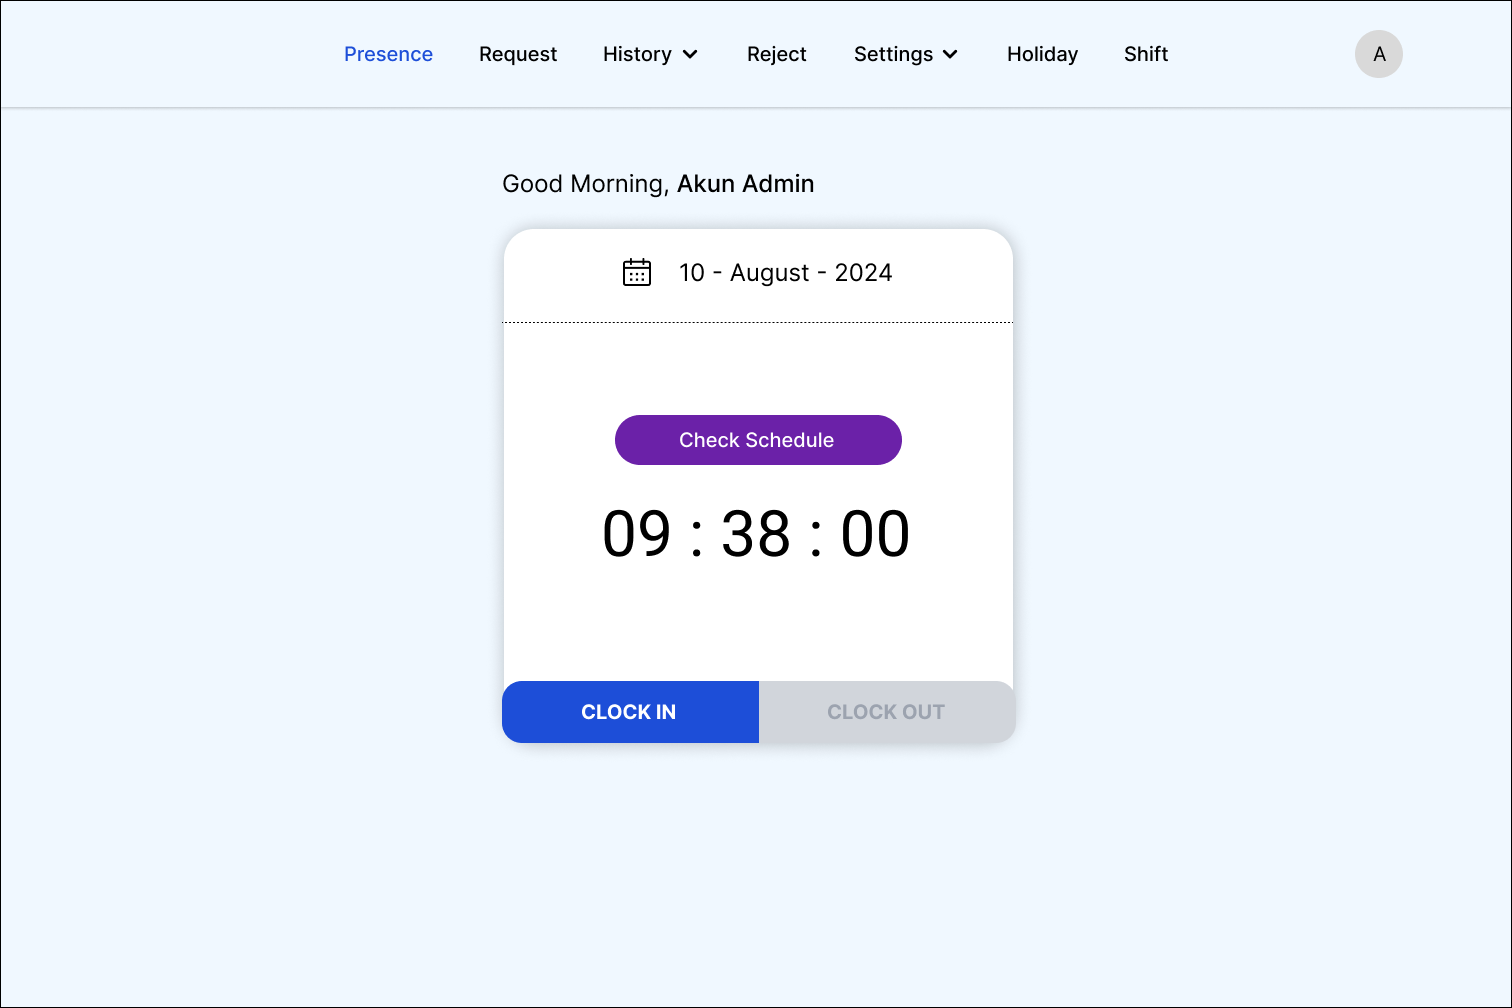
\includegraphics[width=13cm]{Gambar/bab2/mockups/menu-utama.png}
    \caption{\textit{Mockup} Menu Utama}
    \label{fig:mockup-menu-utama}
\end{figure}
\FloatBarrier


\begin{figure}[H]
	\centering
	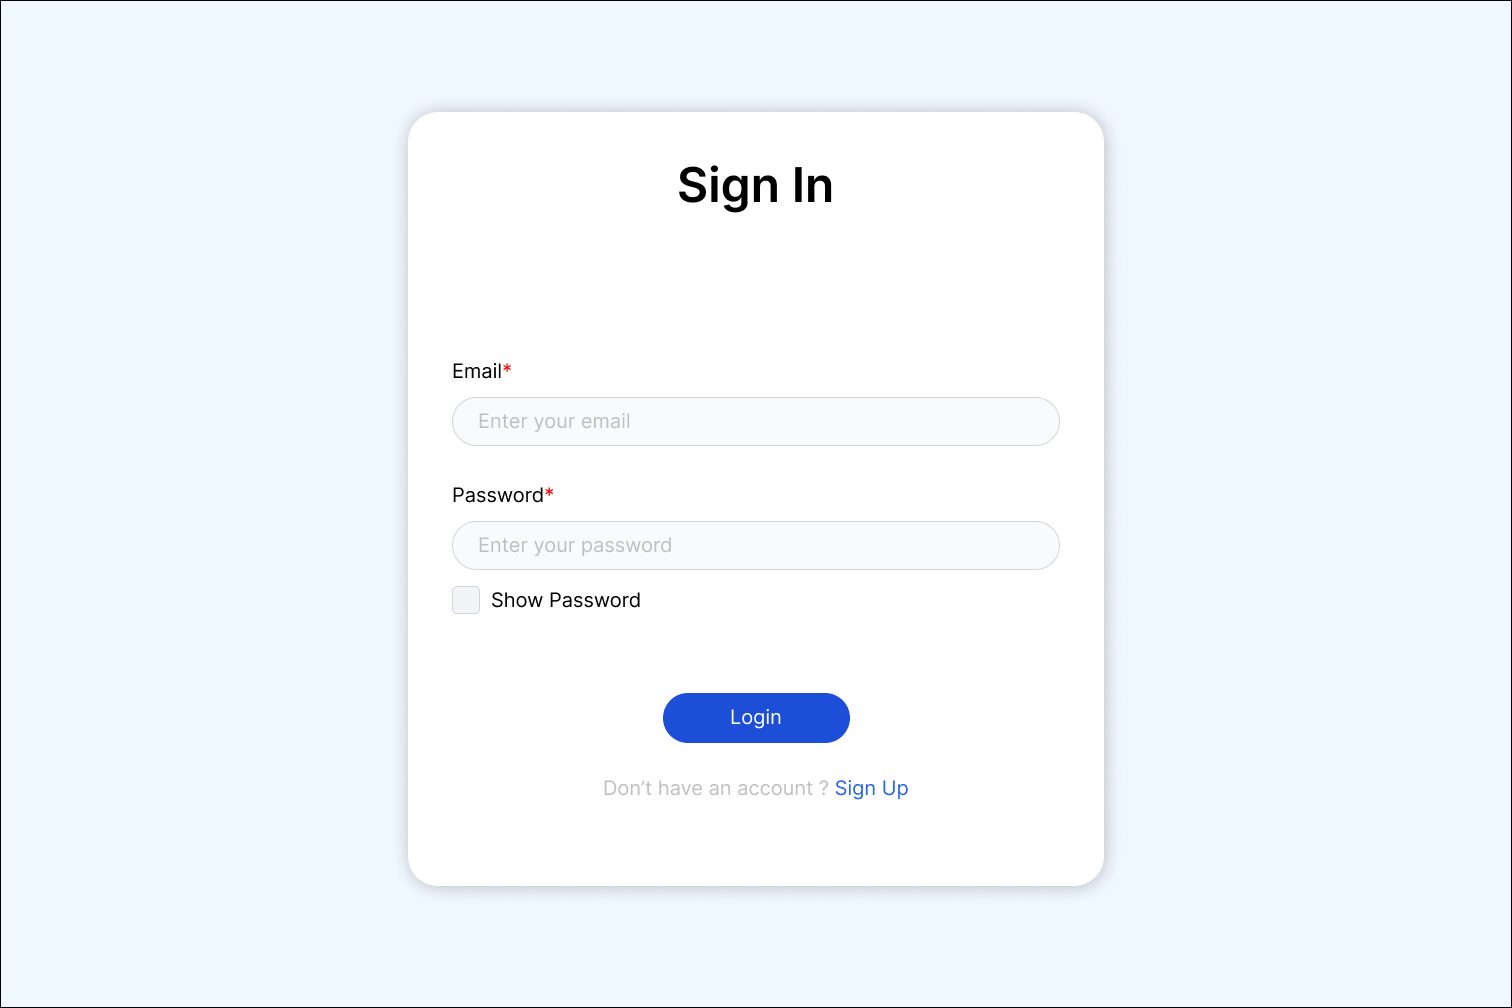
\includegraphics[width=13cm]{Gambar/bab2/mockups/menu-login.png}
	\caption{\textit{Mockup} Menu \textit{Login}}
	\label{fig:mockup-menu-login}
\end{figure}
\FloatBarrier

\begin{figure}[H]
	\centering
	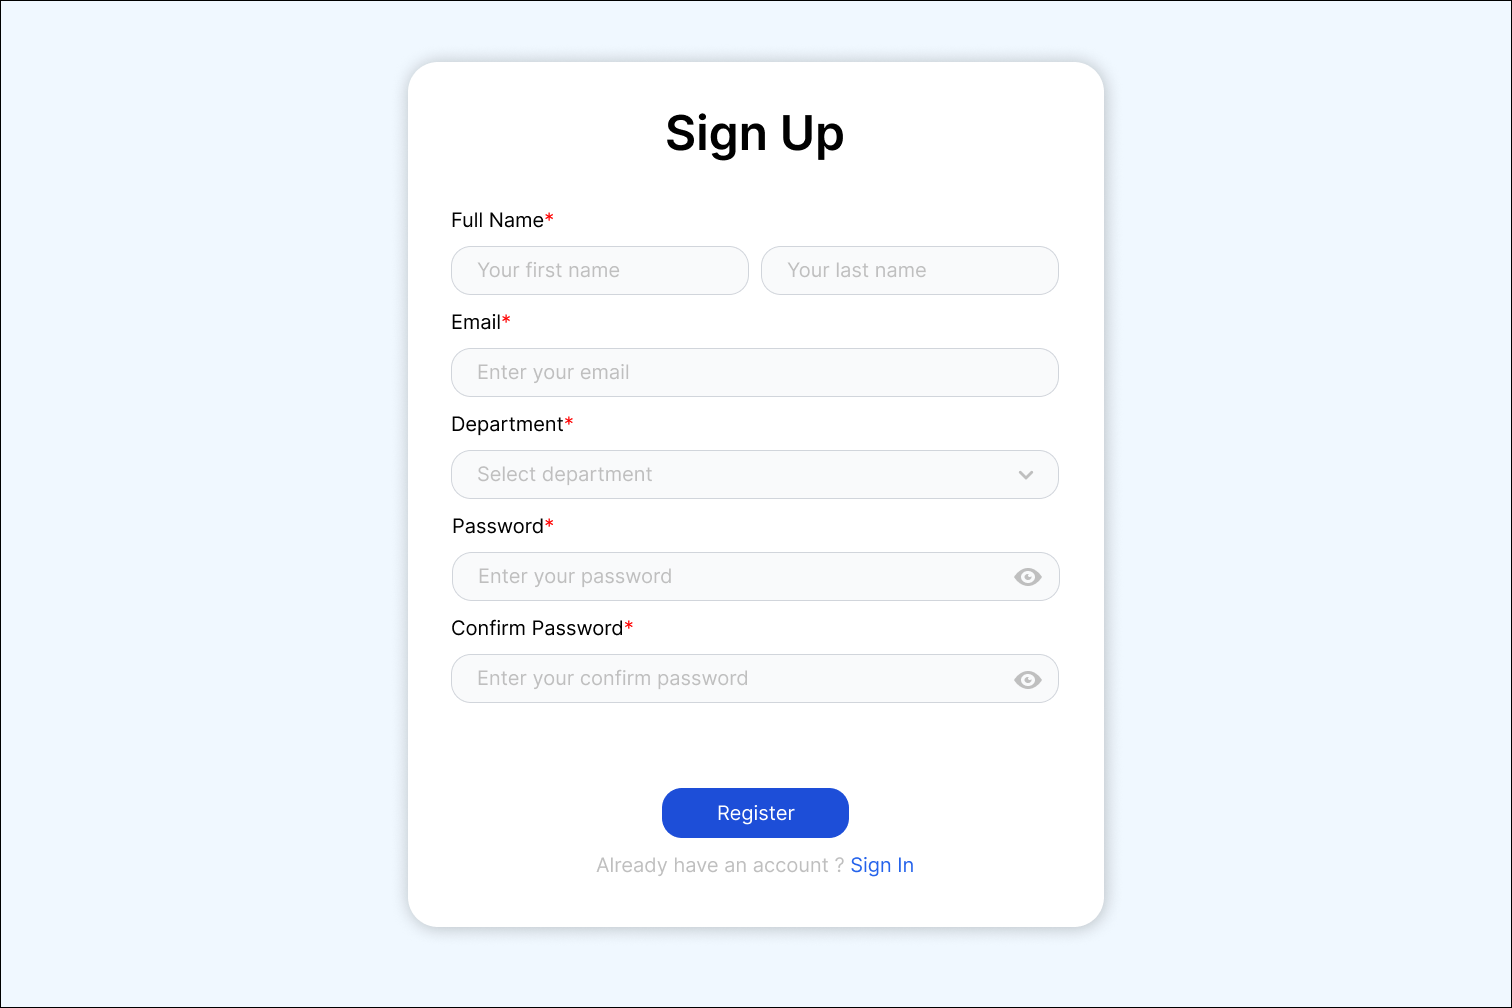
\includegraphics[width=13cm]{Gambar/bab2/mockups/menu-registrasi-akun.png}
	\caption{\textit{Mockup} Menu Registrasi Akun}
	\label{fig:mockup-menu-registrasi-akun}
\end{figure}
\FloatBarrier

\begin{figure}[H]
	\centering
	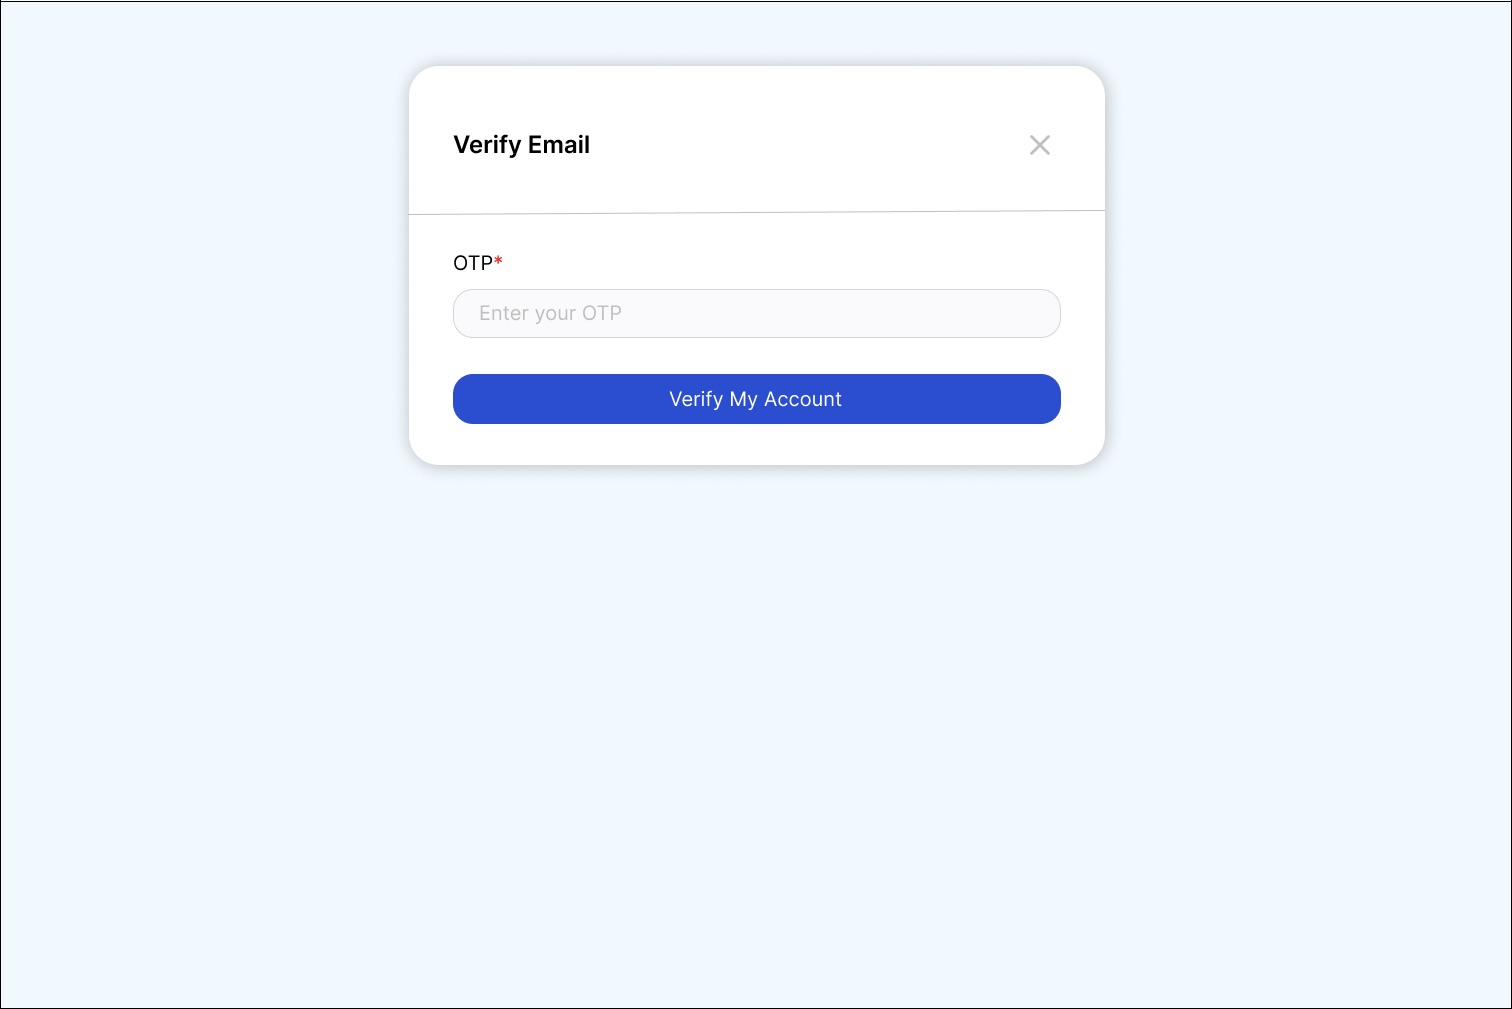
\includegraphics[width=13cm]{Gambar/bab2/mockups/menu-verifikasi-email.png}
	\caption{\textit{Mockup} Menu Verifikasi \textit{Email}}
	\label{fig:mockup-menu-verifikasi-email}
\end{figure}
\FloatBarrier

\begin{figure}[H]
	\centering
	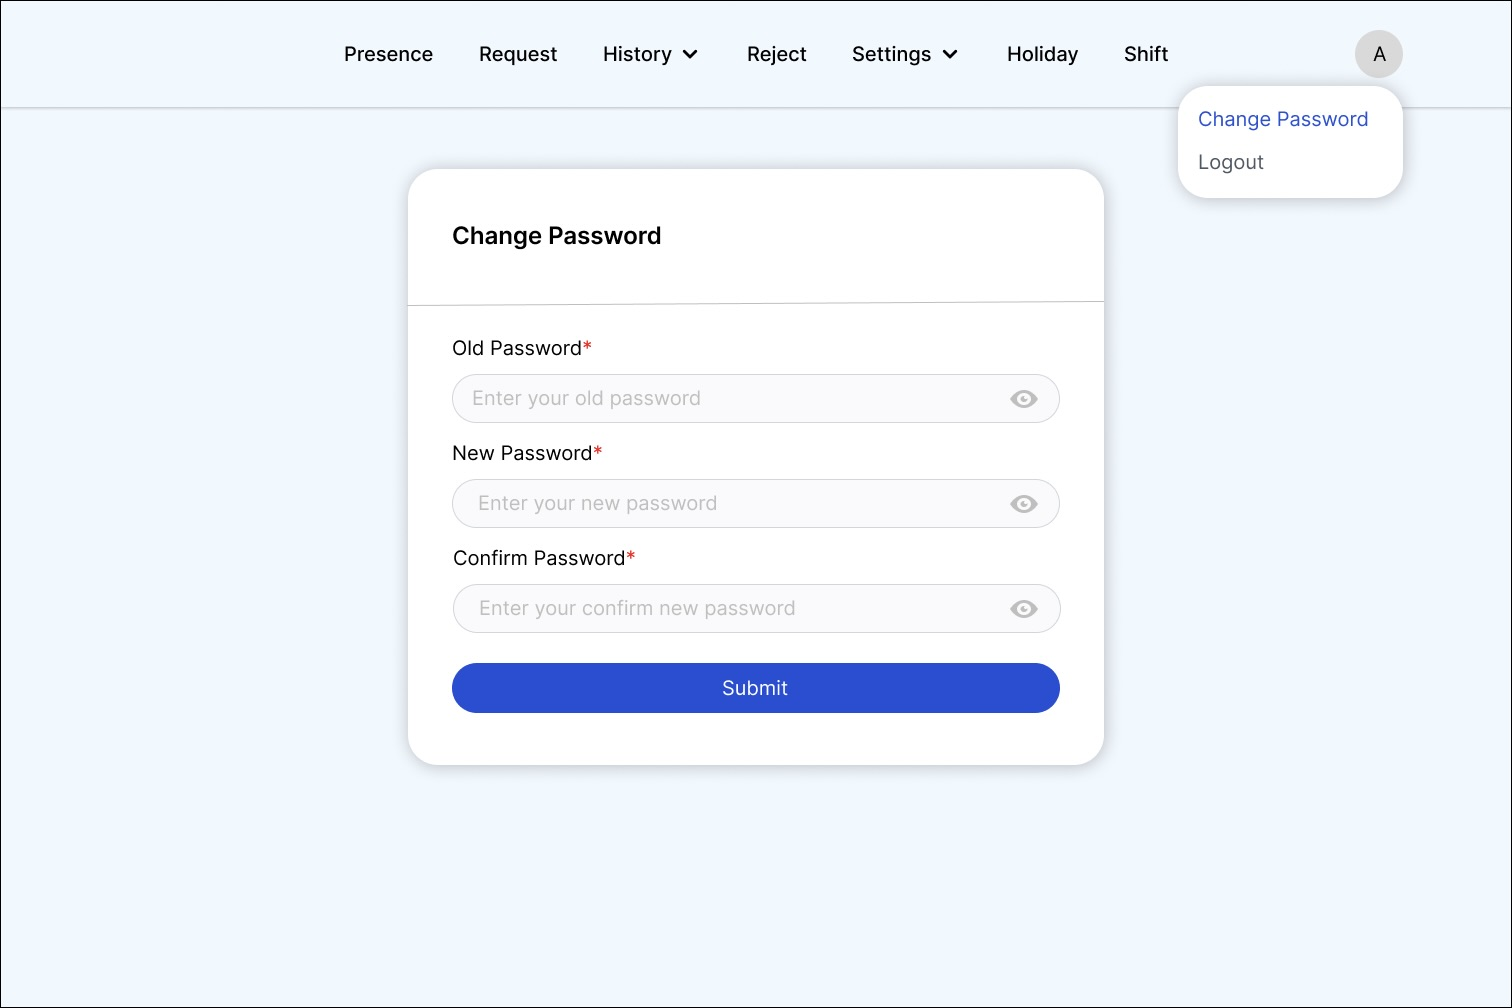
\includegraphics[width=13cm]{Gambar/bab2/mockups/menu-ganti-password.png}
	\caption{\textit{Mockup} Menu Ganti Password}
	\label{fig:mockup-menu-ganti-password}
\end{figure}
\FloatBarrier

\begin{figure}[H]
	\centering
	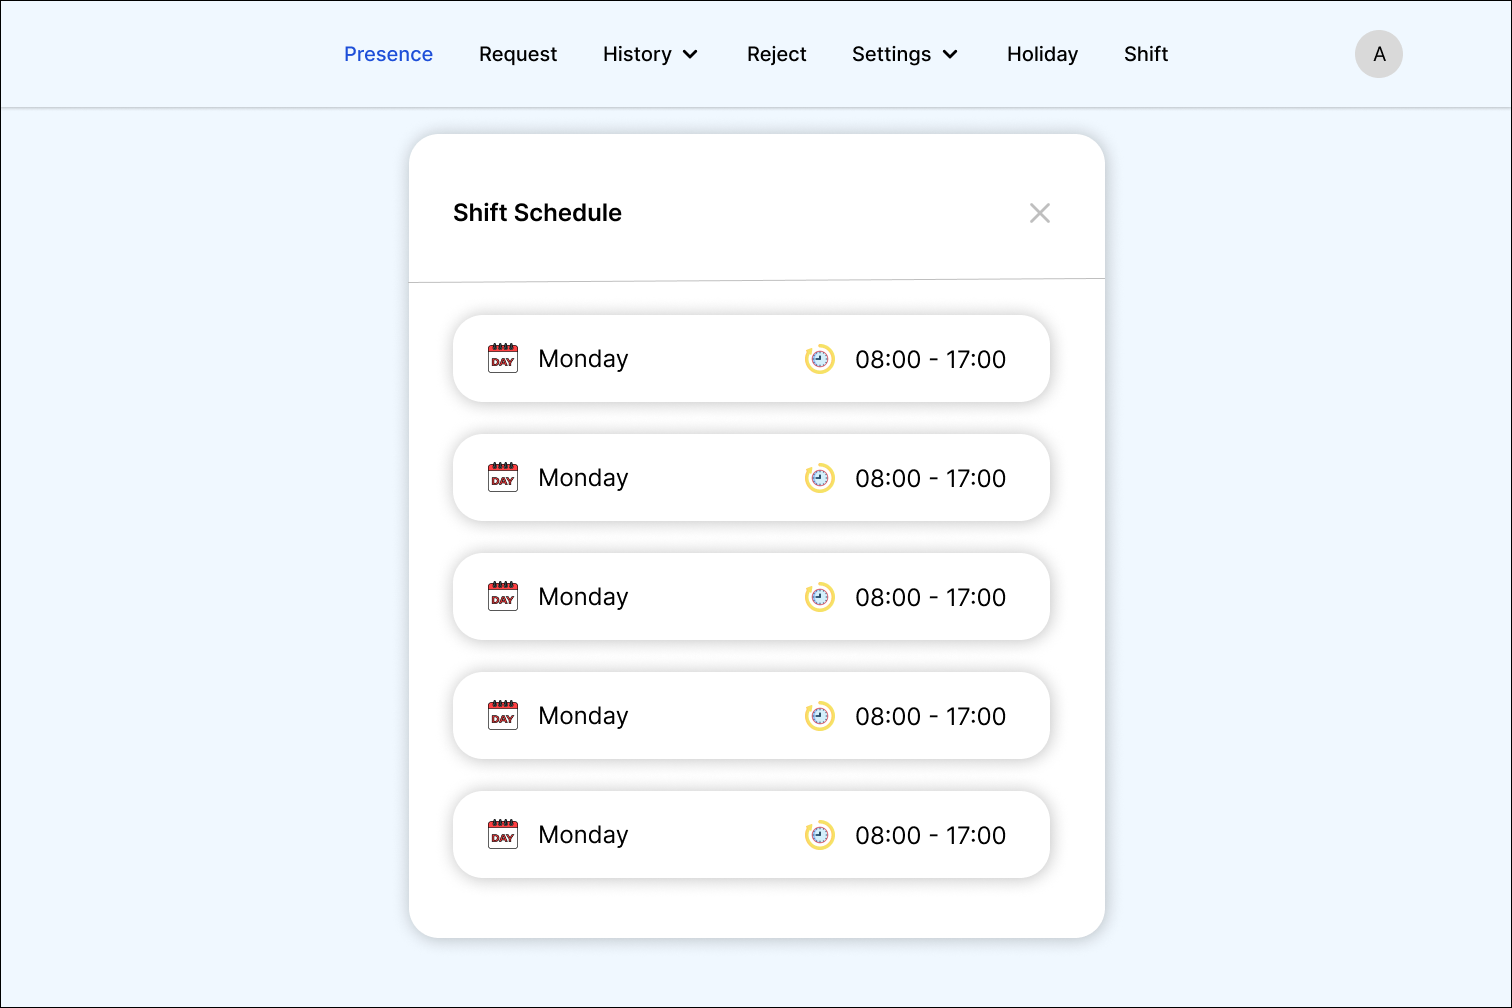
\includegraphics[width=13cm]{Gambar/bab2/mockups/menu-jadwal-shift.png}
	\caption{\textit{Mockup} Menu Jadwal \textit{Shift}}
	\label{fig:mockup-menu-jadwal-shift}
\end{figure}
\FloatBarrier

\begin{figure}[H]
	\centering
	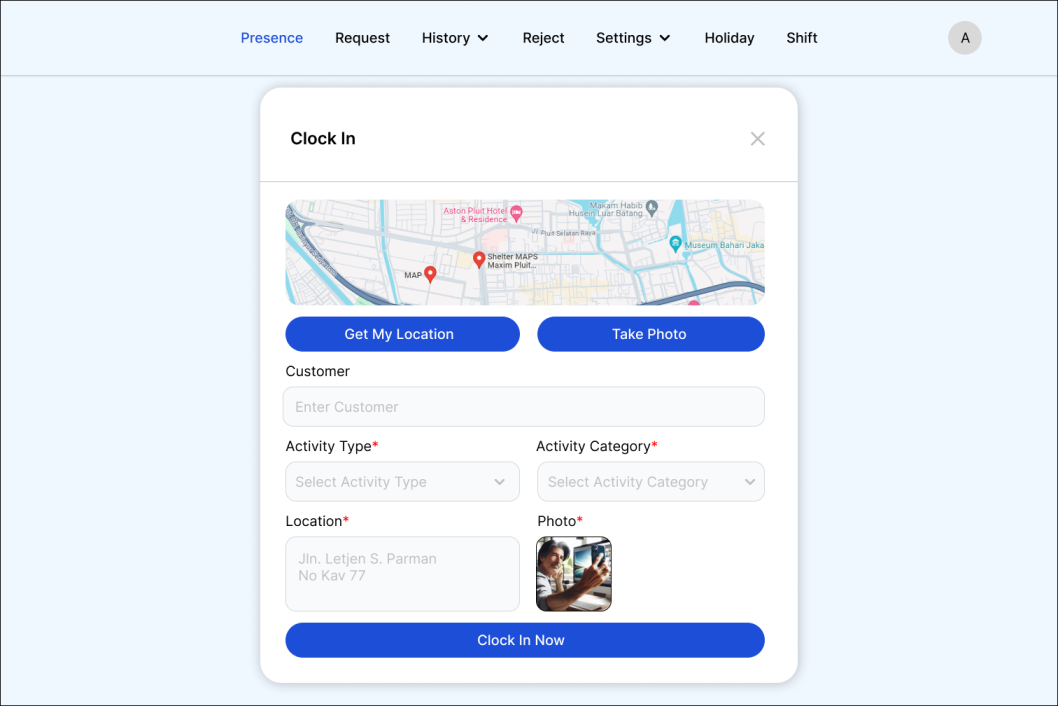
\includegraphics[width=13cm]{Gambar/bab2/mockups/menu-clock-in.png}
	\caption{\textit{Mockup} Menu \textit{Clock In}}
	\label{fig:mockup-menu-clock-in}
\end{figure}
\FloatBarrier

\begin{figure}[H]
	\centering
	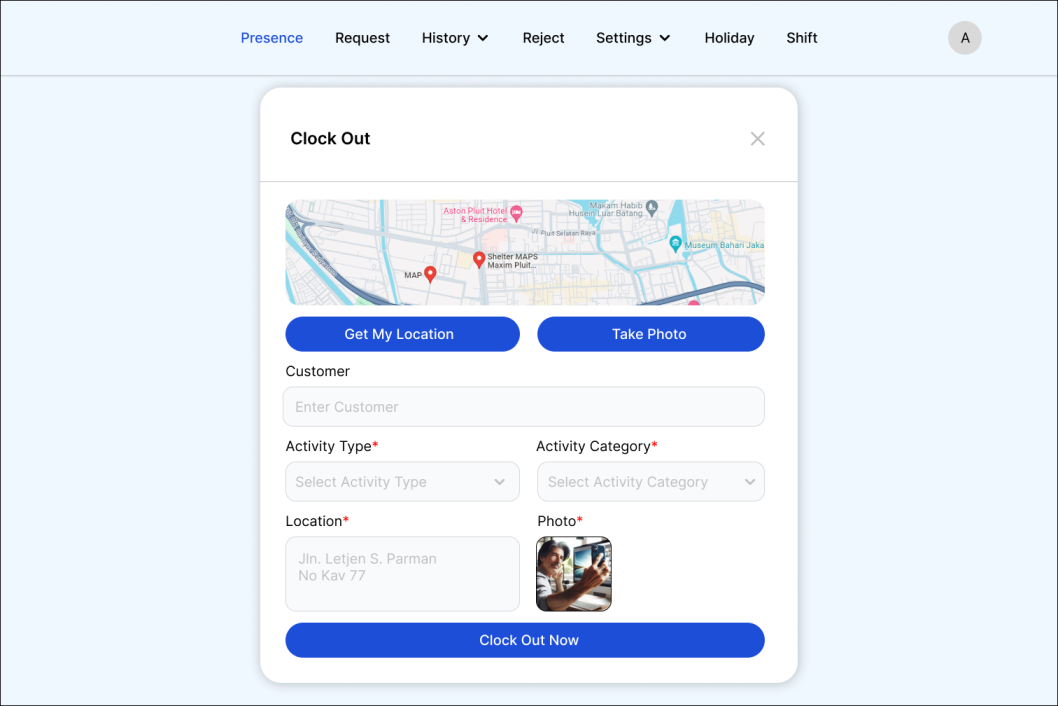
\includegraphics[width=13cm]{Gambar/bab2/mockups/menu-clock-out.png}
	\caption{\textit{Mockup} Menu \textit{Clock Out}}
	\label{fig:mockup-menu-clock-out}
\end{figure}
\FloatBarrier

\begin{figure}[H]
	\centering
	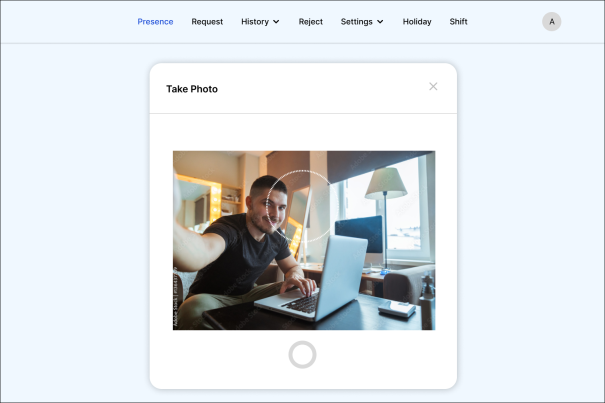
\includegraphics[width=13cm]{Gambar/bab2/mockups/menu-kamera.png}
	\caption{\textit{Mockup} Menu Kamera}
	\label{fig:mockup-menu-kamera}
\end{figure}
\FloatBarrier

\begin{figure}[H]
	\centering
	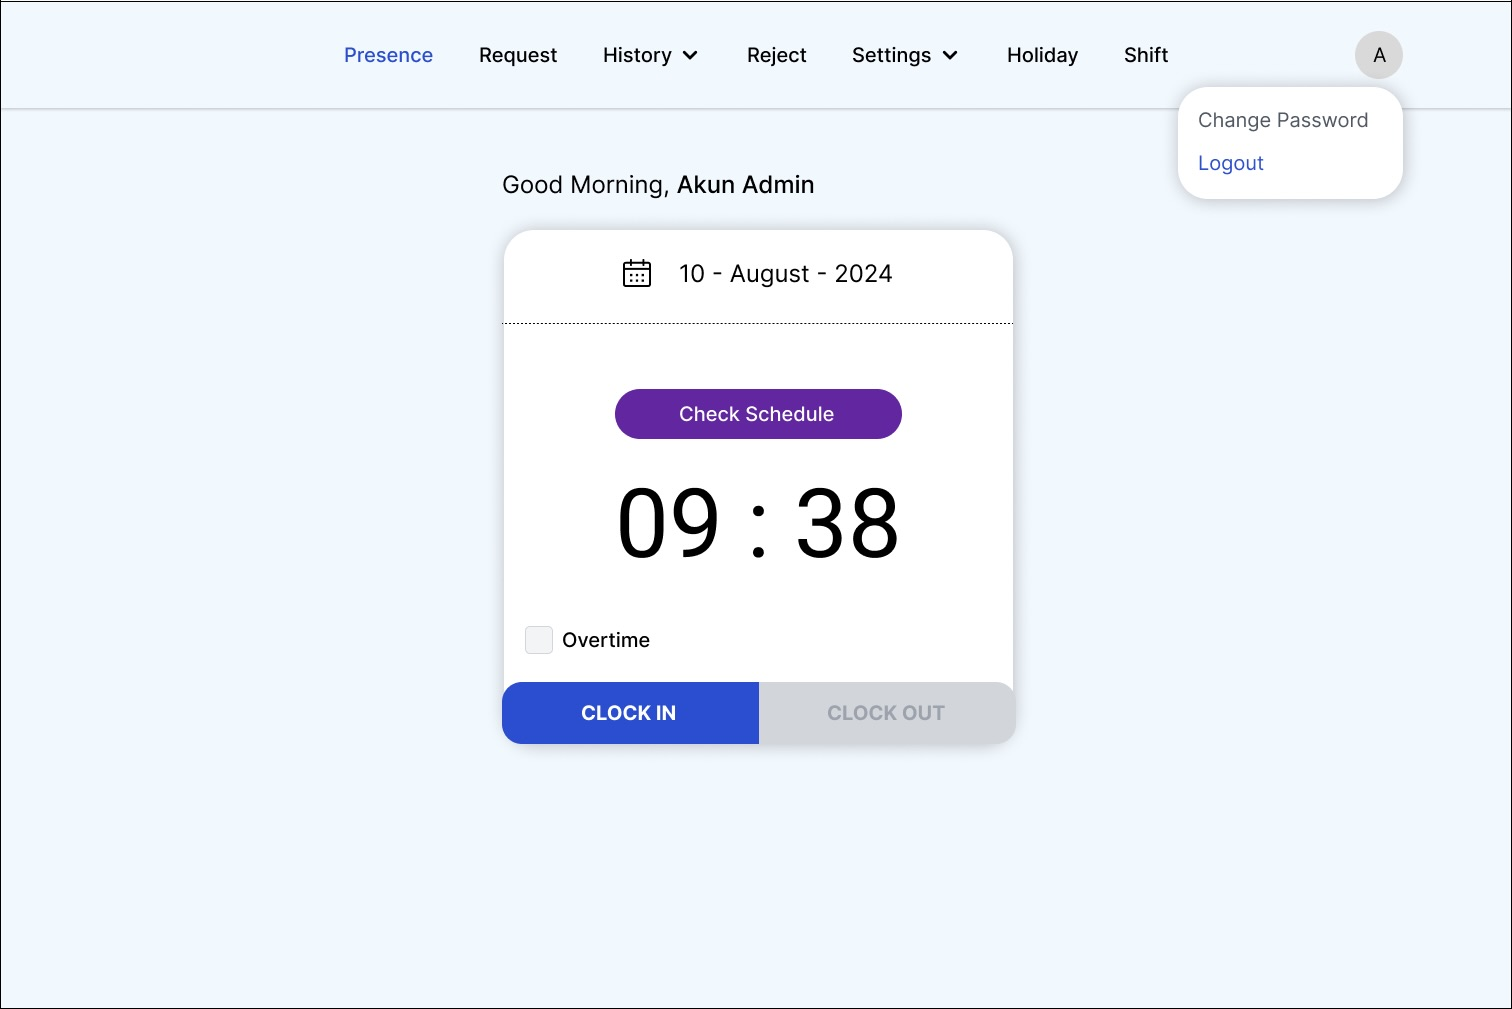
\includegraphics[width=13cm]{Gambar/bab2/mockups/menu-profil.png}
	\caption{\textit{Mockup} Menu Profil}
	\label{fig:mockup-menu-profil}
\end{figure}
\FloatBarrier

\begin{figure}[H]
	\centering
	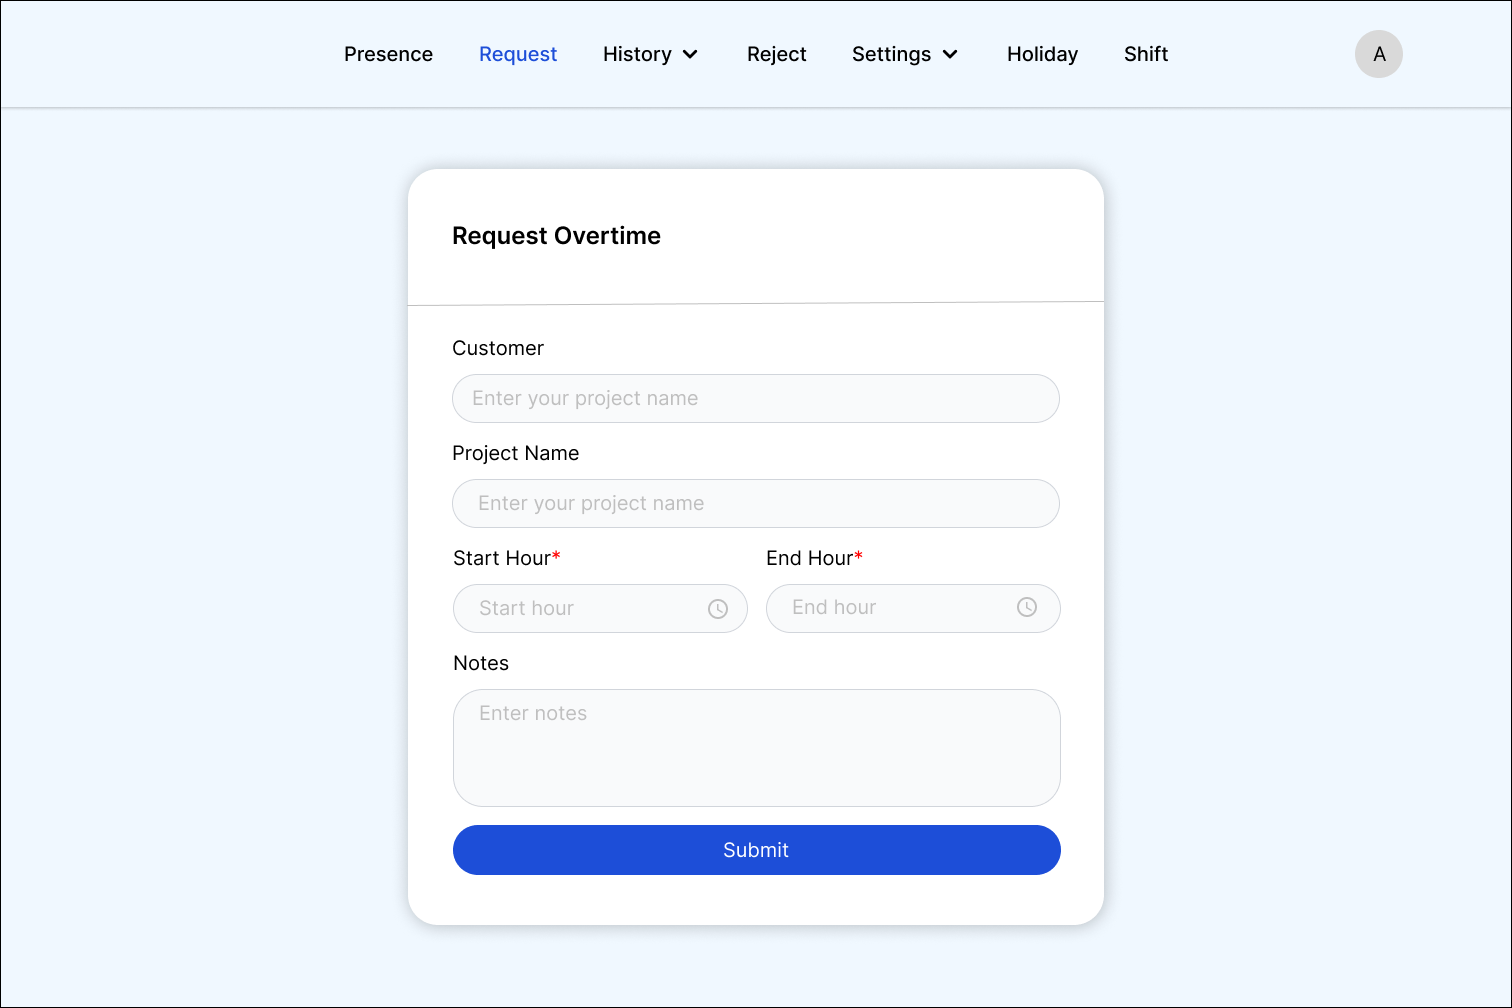
\includegraphics[width=13cm]{Gambar/bab2/mockups/menu-pengajuan-lembur.png}
	\caption{\textit{Mockup} Menu Pengajuan Lembur}
	\label{fig:mockup-menu-pengajuan-lembur}
\end{figure}
\FloatBarrier

\begin{figure}[H]
	\centering
	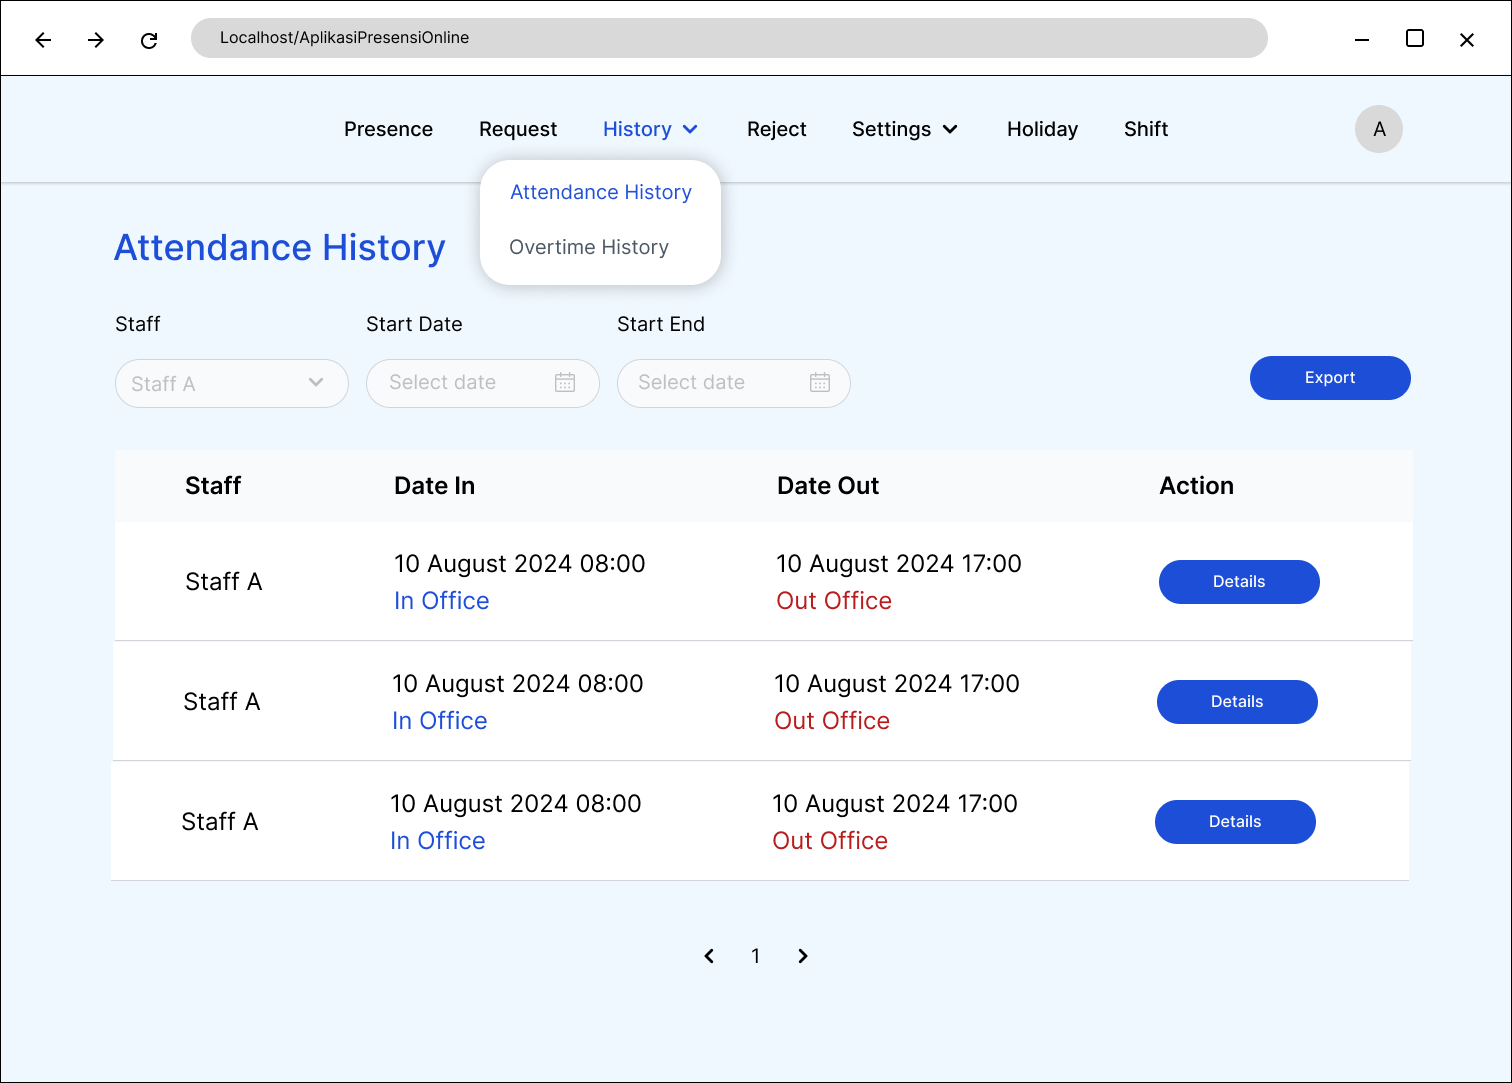
\includegraphics[width=13cm]{Gambar/bab2/mockups/menu-riwayat-presensi.png}
	\caption{\textit{Mockup} Menu Riwayat Presensi}
	\label{fig:mockup-menu-riwayat-presensi}
\end{figure}
\FloatBarrier

\begin{figure}[H]
	\centering
	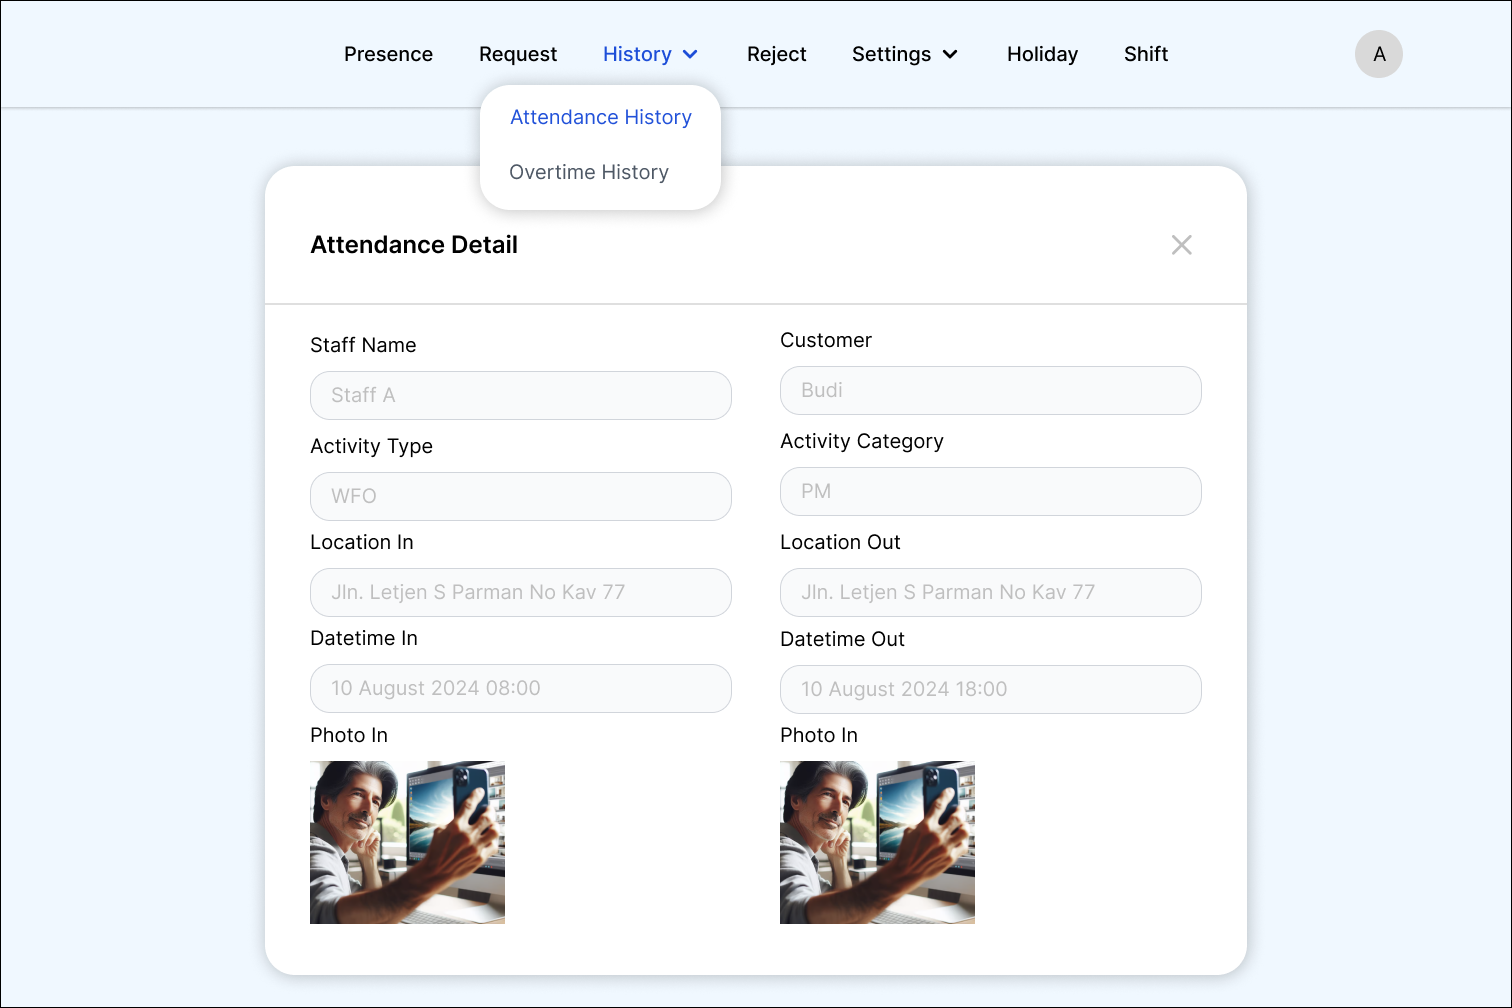
\includegraphics[width=13cm]{Gambar/bab2/mockups/menu-detail-presensi.png}
	\caption{\textit{Mockup} Menu Detail Presensi}
	\label{fig:mockup-menu-detail-presensi}
\end{figure}
\FloatBarrier

\begin{figure}[H]
	\centering
	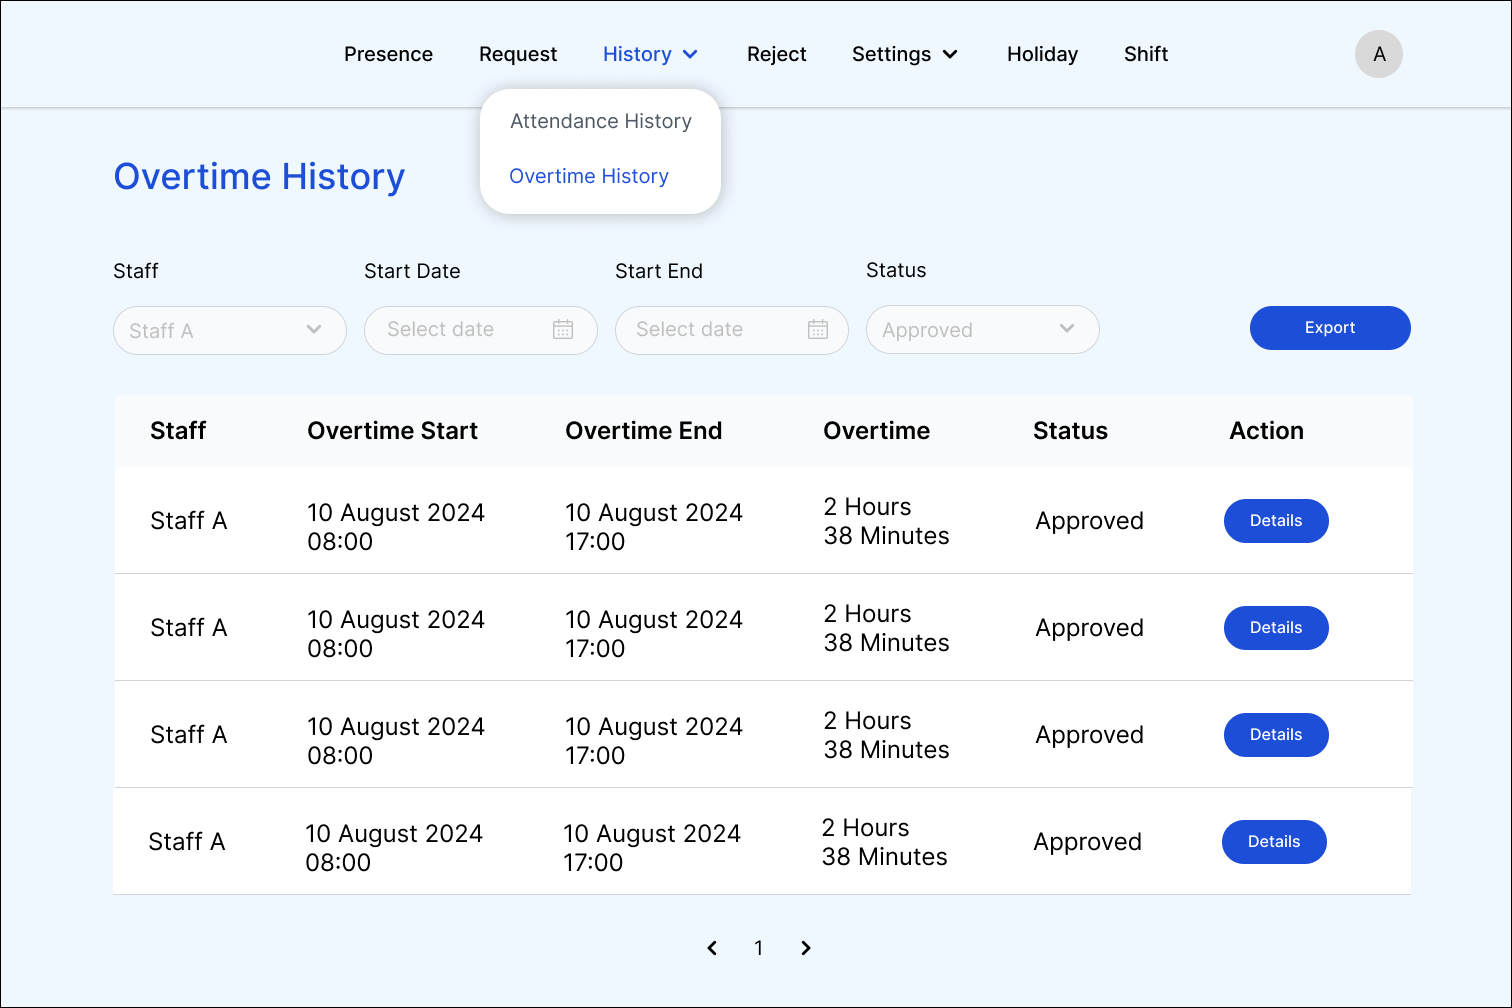
\includegraphics[width=13cm]{Gambar/bab2/mockups/menu-riwayat-lembur.png}
	\caption{\textit{Mockup} Menu Riwayat Lembur}
	\label{fig:mockup-menu-riwayat-lembur}
\end{figure}
\FloatBarrier

\begin{figure}[H]
	\centering
	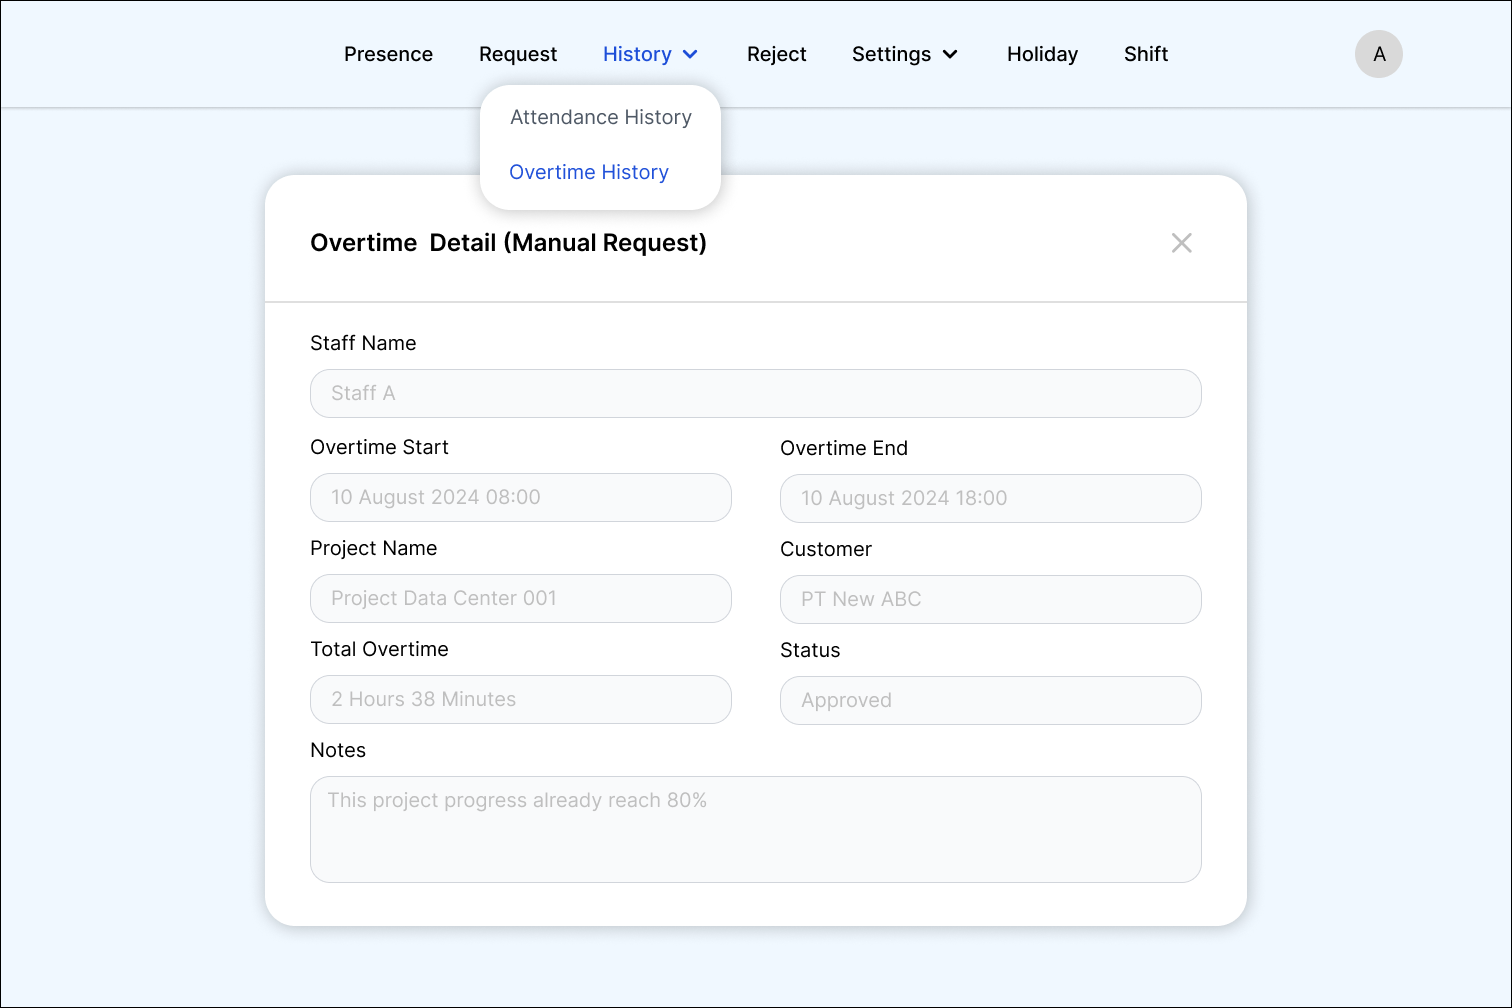
\includegraphics[width=13cm]{Gambar/bab2/mockups/menu-detail-lembur.png}
	\caption{\textit{Mockup} Menu Detail Lembur}
	\label{fig:mockup-menu-detail-lembur}
\end{figure}
\FloatBarrier

\begin{figure}[H]
	\centering
	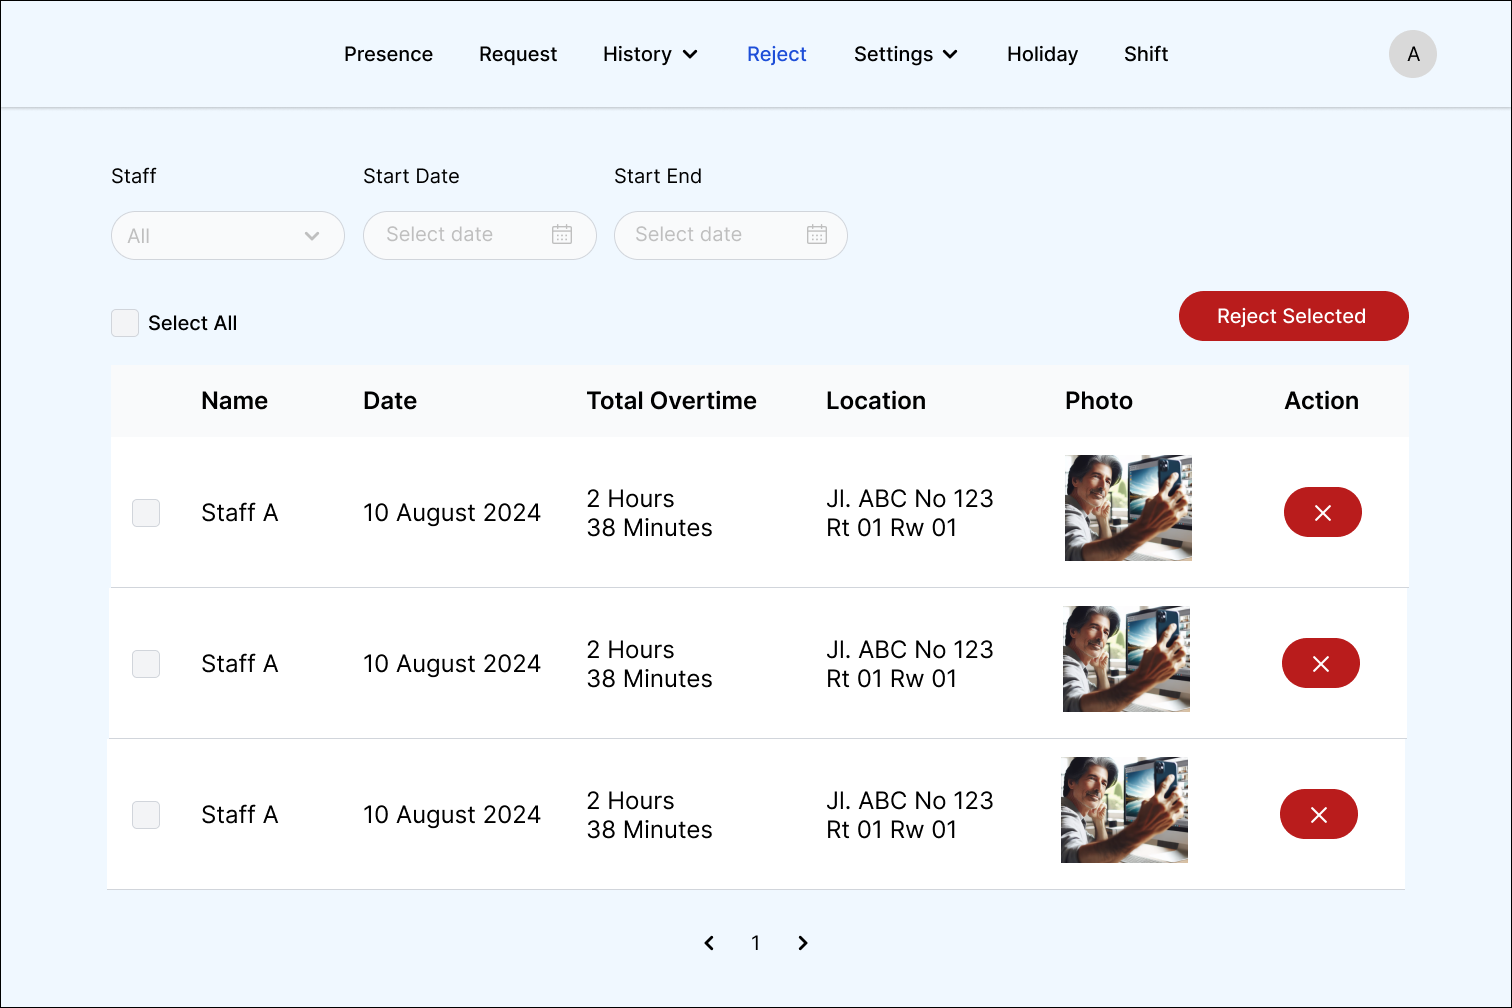
\includegraphics[width=13cm]{Gambar/bab2/mockups/menu-reject-lembur.png}
	\caption{\textit{Mockup} Menu \textit{Reject} Lembur}
	\label{fig:mockup-menu-reject-lembur}
\end{figure}
\FloatBarrier

\begin{figure}[H]
	\centering
	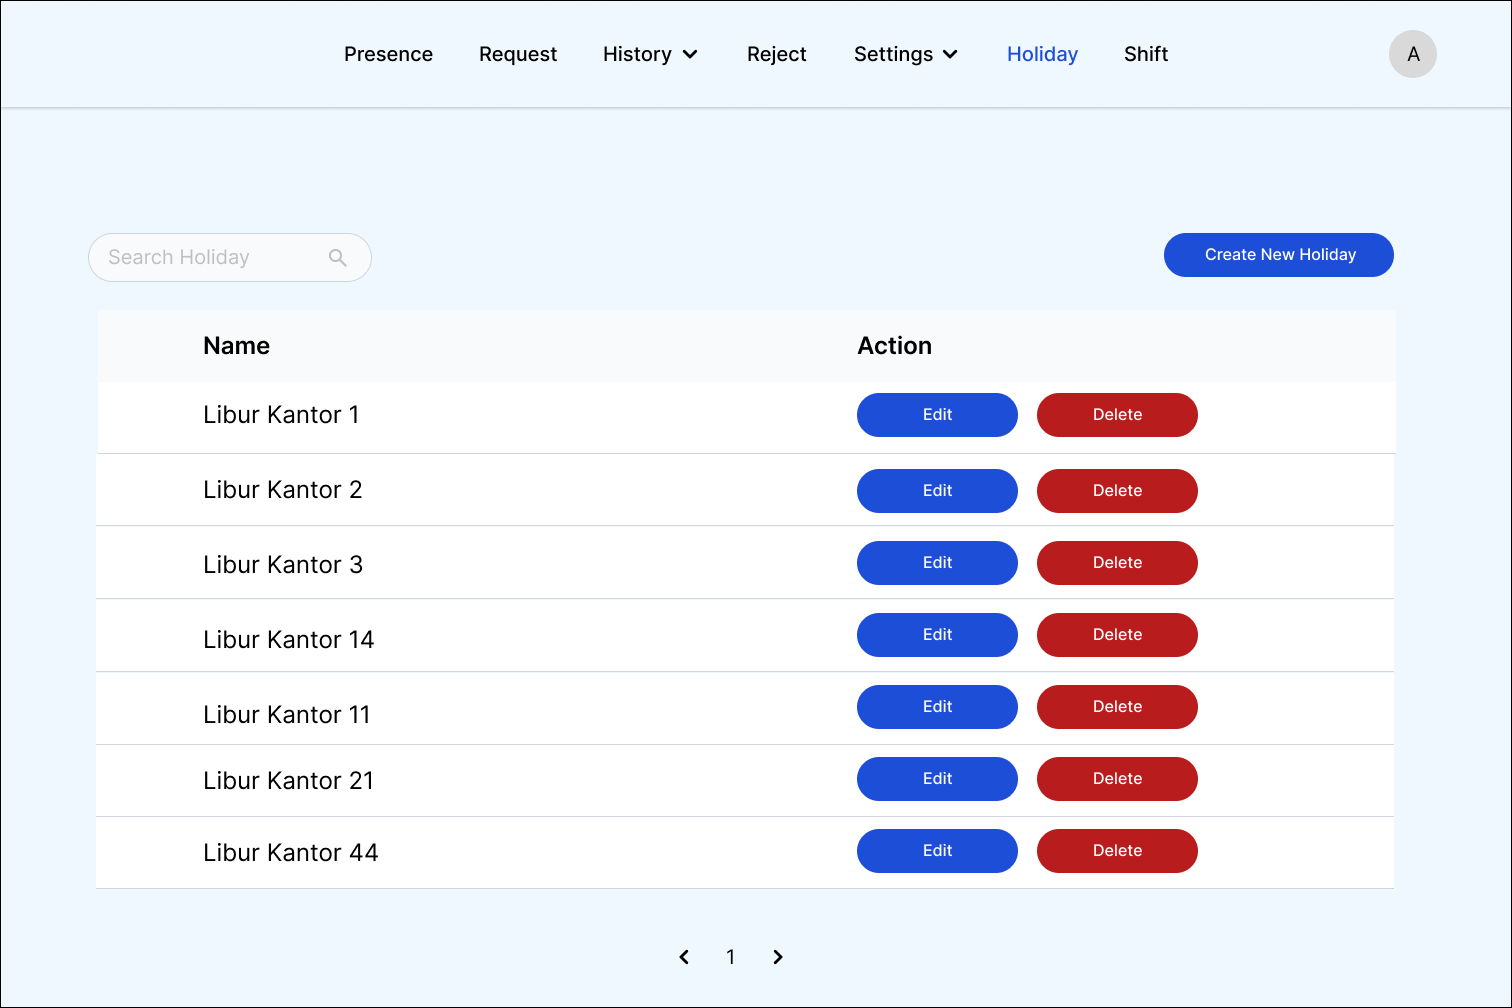
\includegraphics[width=13cm]{Gambar/bab2/mockups/menu-libur.png}
	\caption{\textit{Mockup} Menu Libur}
	\label{fig:mockup-menu-libur}
\end{figure}
\FloatBarrier

\begin{figure}[H]
	\centering
	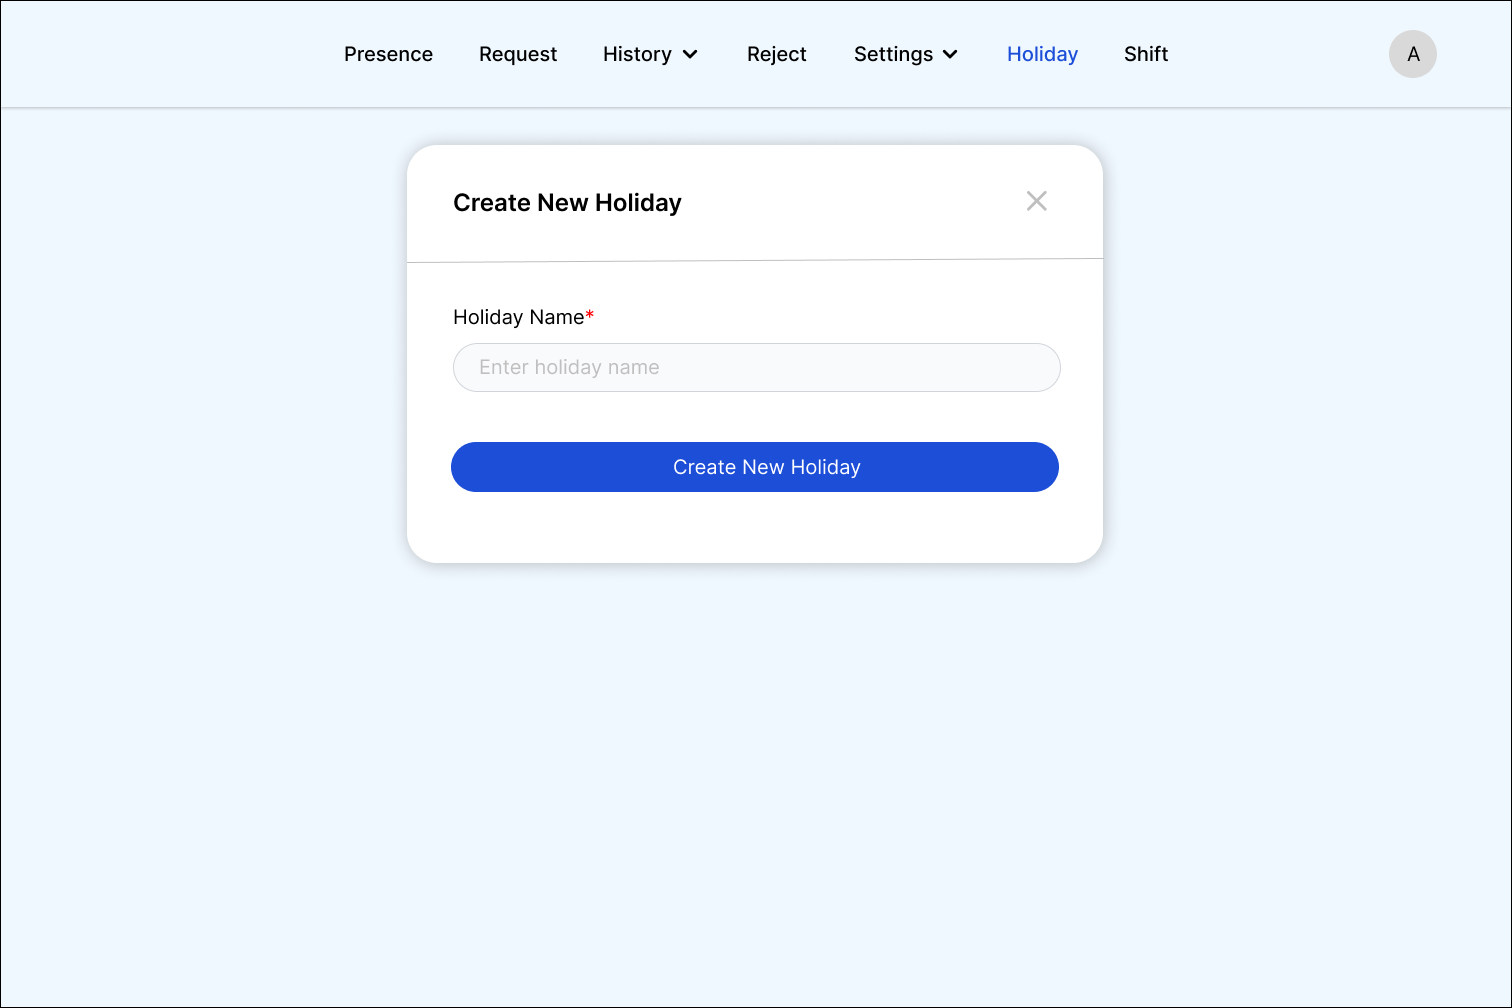
\includegraphics[width=13cm]{Gambar/bab2/mockups/menu-tambah-libur.png}
	\caption{\textit{Mockup} Menu Tambah Libur}
	\label{fig:mockup-menu-tambah-libur}
\end{figure}
\FloatBarrier

\begin{figure}[H]
	\centering
	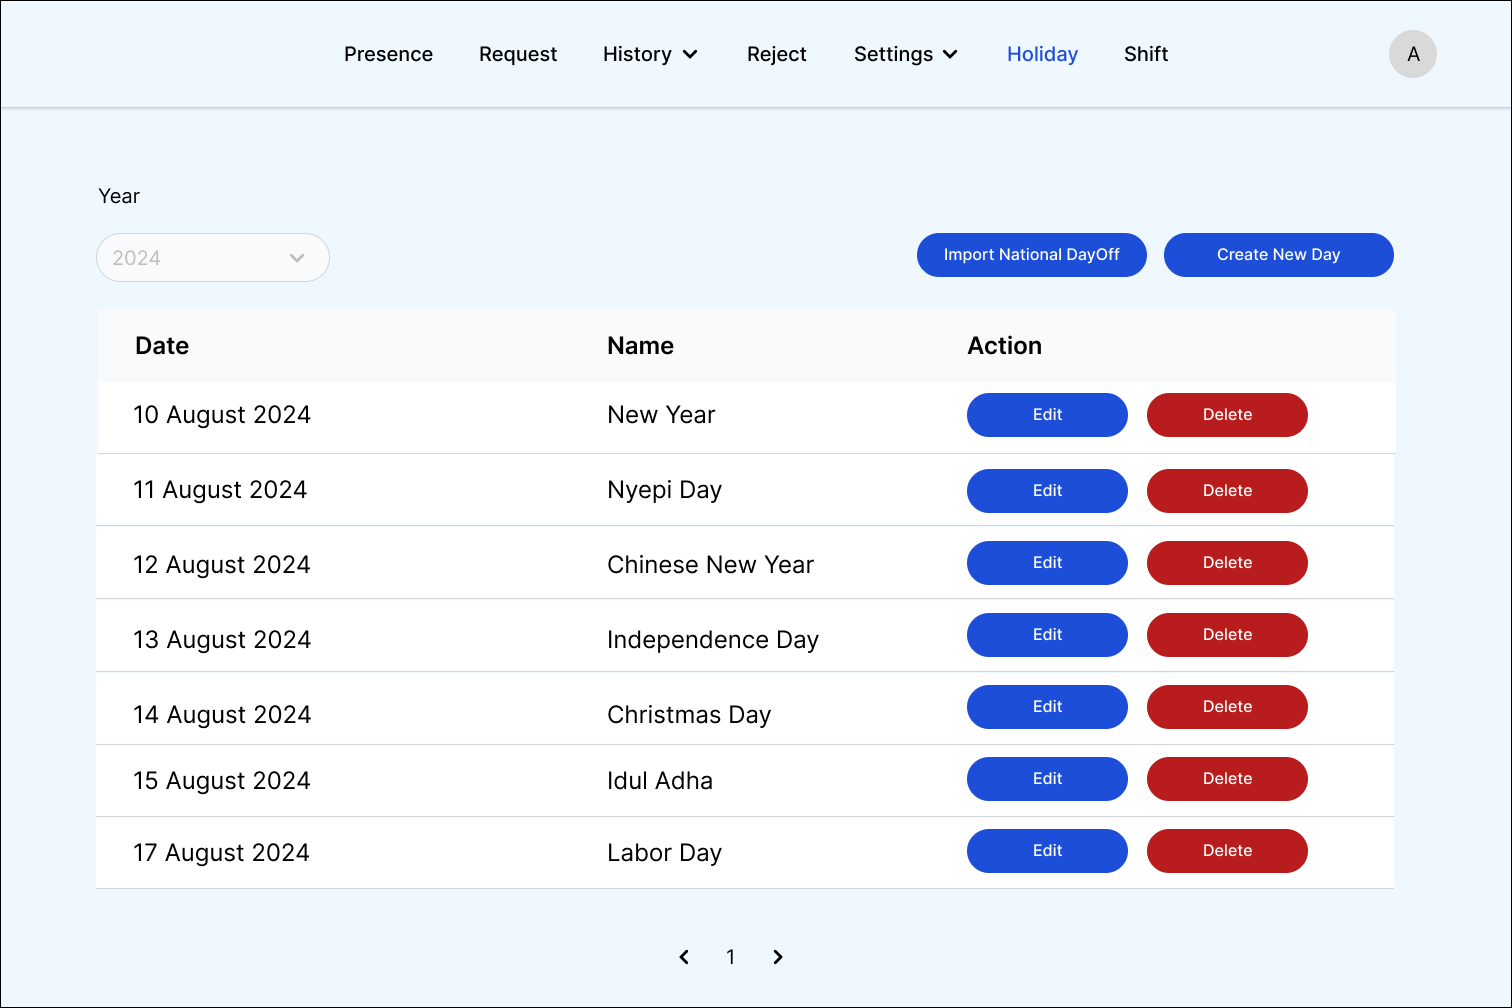
\includegraphics[width=13cm]{Gambar/bab2/mockups/menu-hari-libur.png}
	\caption{\textit{Mockup} Menu Hari Libur}
	\label{fig:mockup-menu-hari-libur}
\end{figure}
\FloatBarrier

\begin{figure}[H]
	\centering
	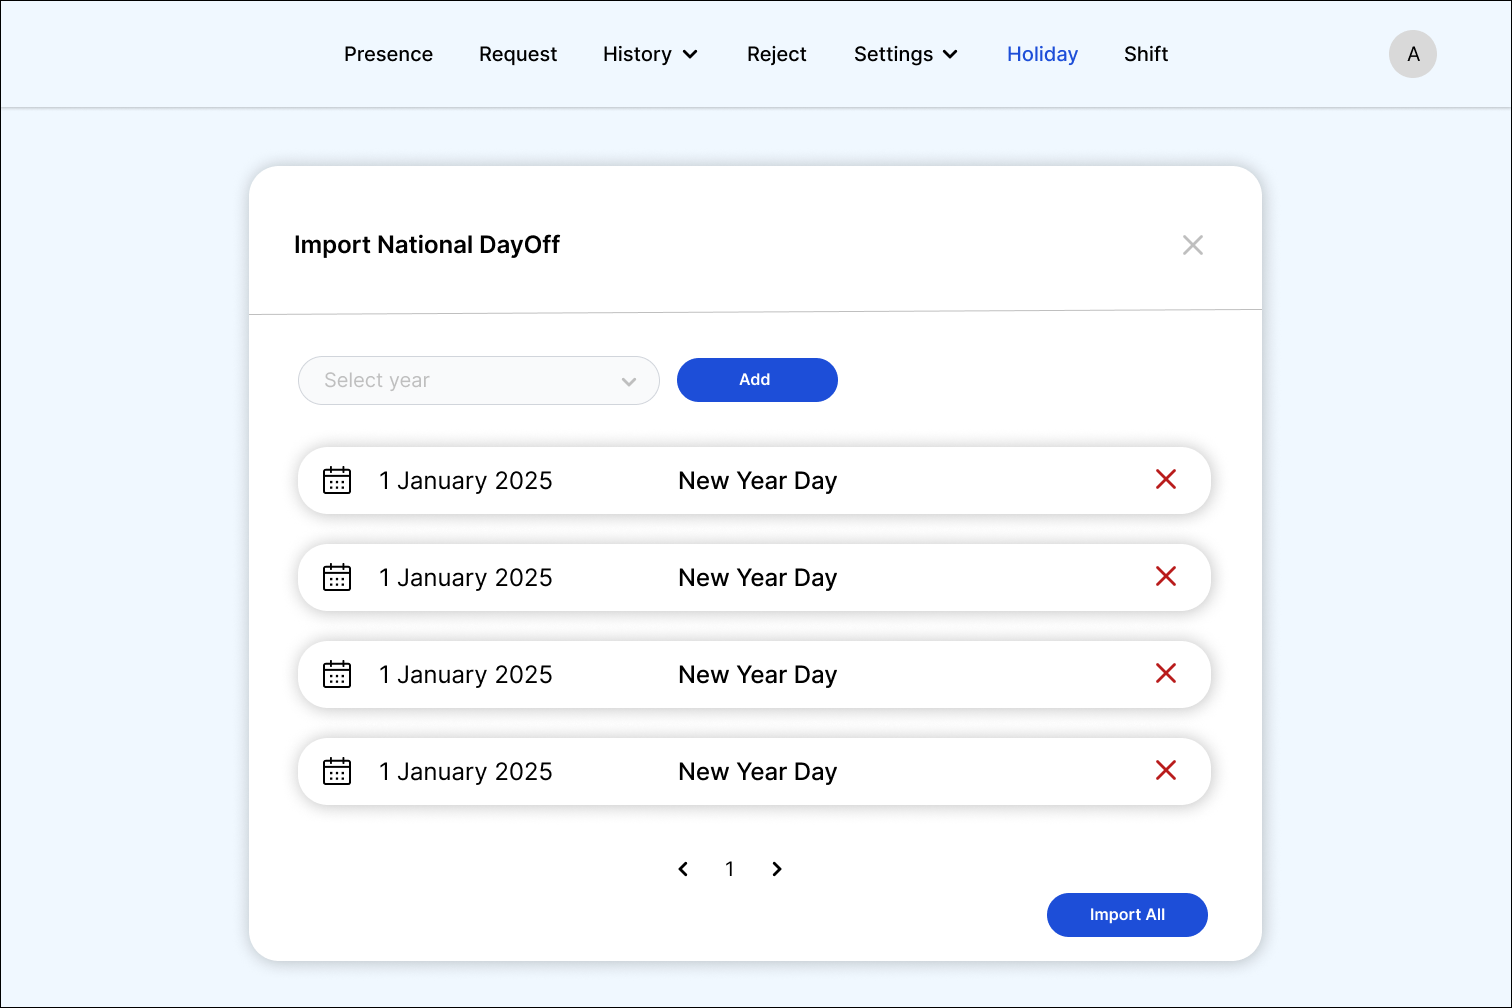
\includegraphics[width=13cm]{Gambar/bab2/mockups/menu-import-libur.png}
	\caption{\textit{Mockup} Menu \textit{Import} Libur}
	\label{fig:mockup-menu-import-libur}
\end{figure}
\FloatBarrier

\begin{figure}[H]
	\centering
	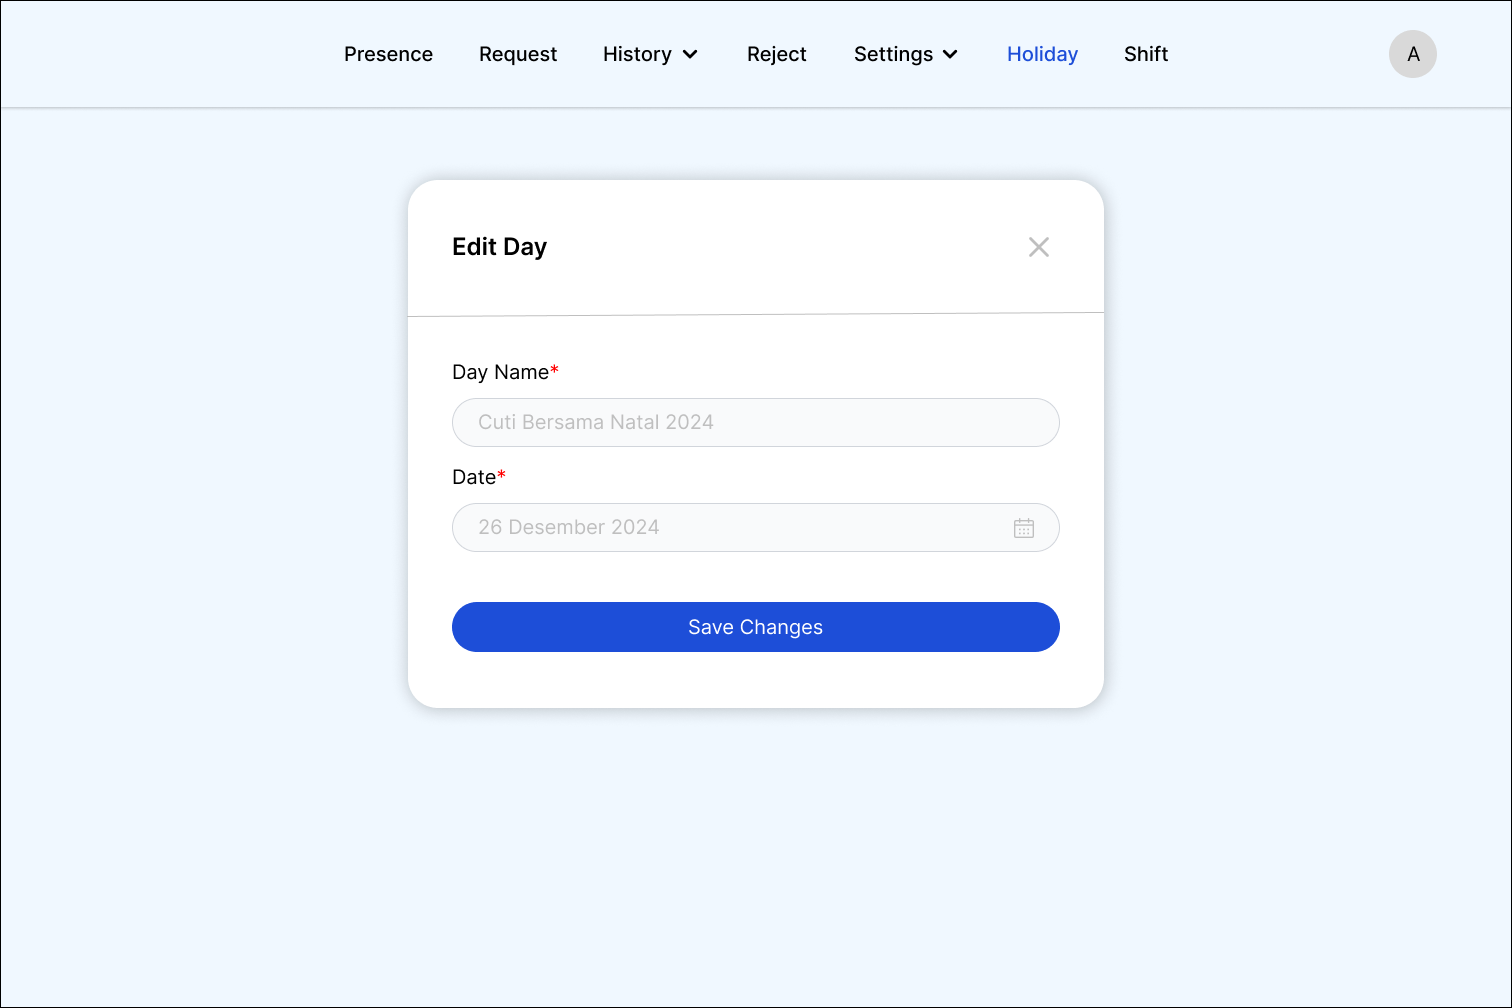
\includegraphics[width=13cm]{Gambar/bab2/mockups/menu-edit-hari-libur.png}
	\caption{\textit{Mockup} Menu \textit{Edit} Hari Libur}
	\label{fig:mockup-menu-edit-hari-libur}
\end{figure}
\FloatBarrier

\begin{figure}[H]
	\centering
	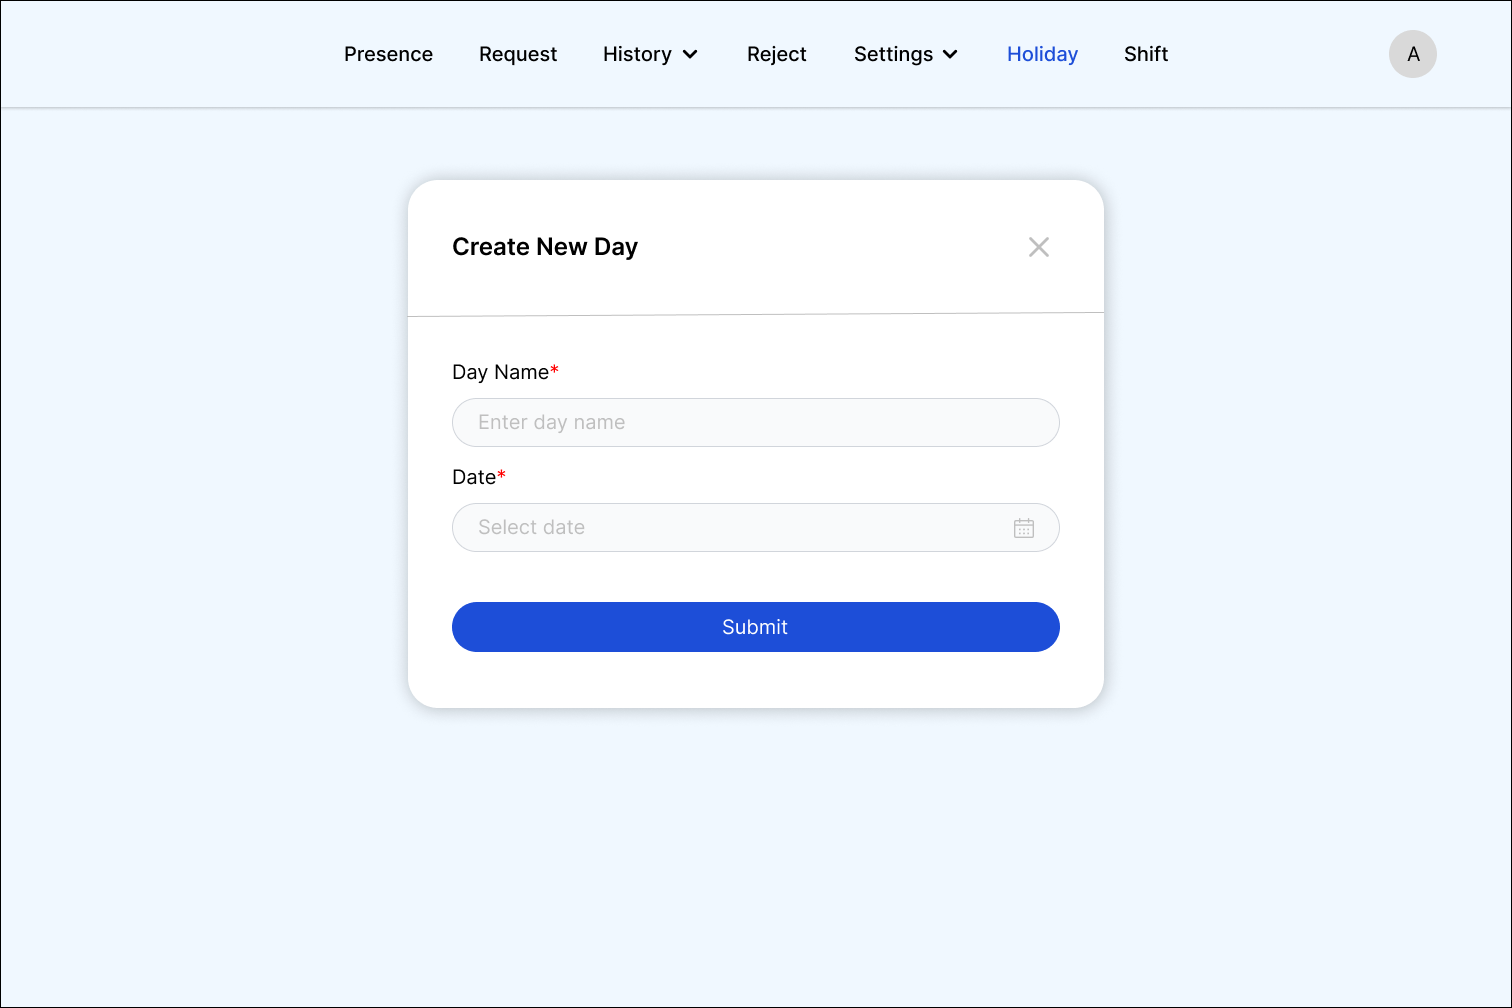
\includegraphics[width=13cm]{Gambar/bab2/mockups/menu-tambah-hari-libur.png}
	\caption{\textit{Mockup} Menu Tambah Hari Libur}
	\label{fig:mockup-menu-tambah-hari-libur}
\end{figure}
\FloatBarrier

\begin{figure}[H]
	\centering
	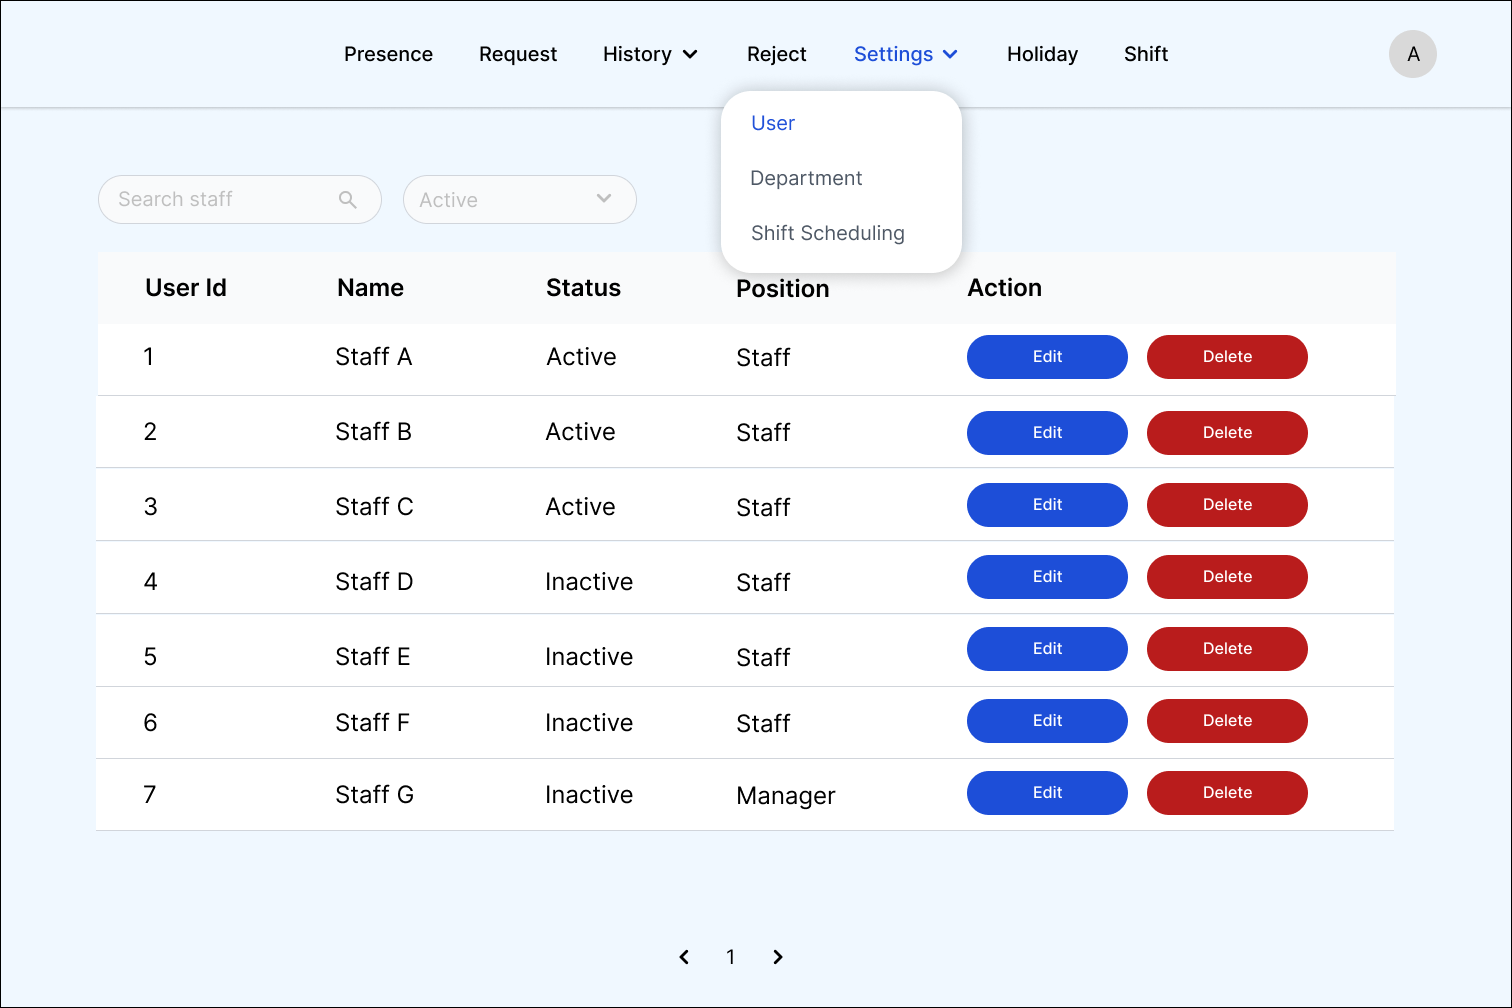
\includegraphics[width=13cm]{Gambar/bab2/mockups/menu-user.png}
	\caption{\textit{Mockup} Menu \textit{User}}
	\label{fig:mockup-menu-user}
\end{figure}
\FloatBarrier

\begin{figure}[H]
	\centering
	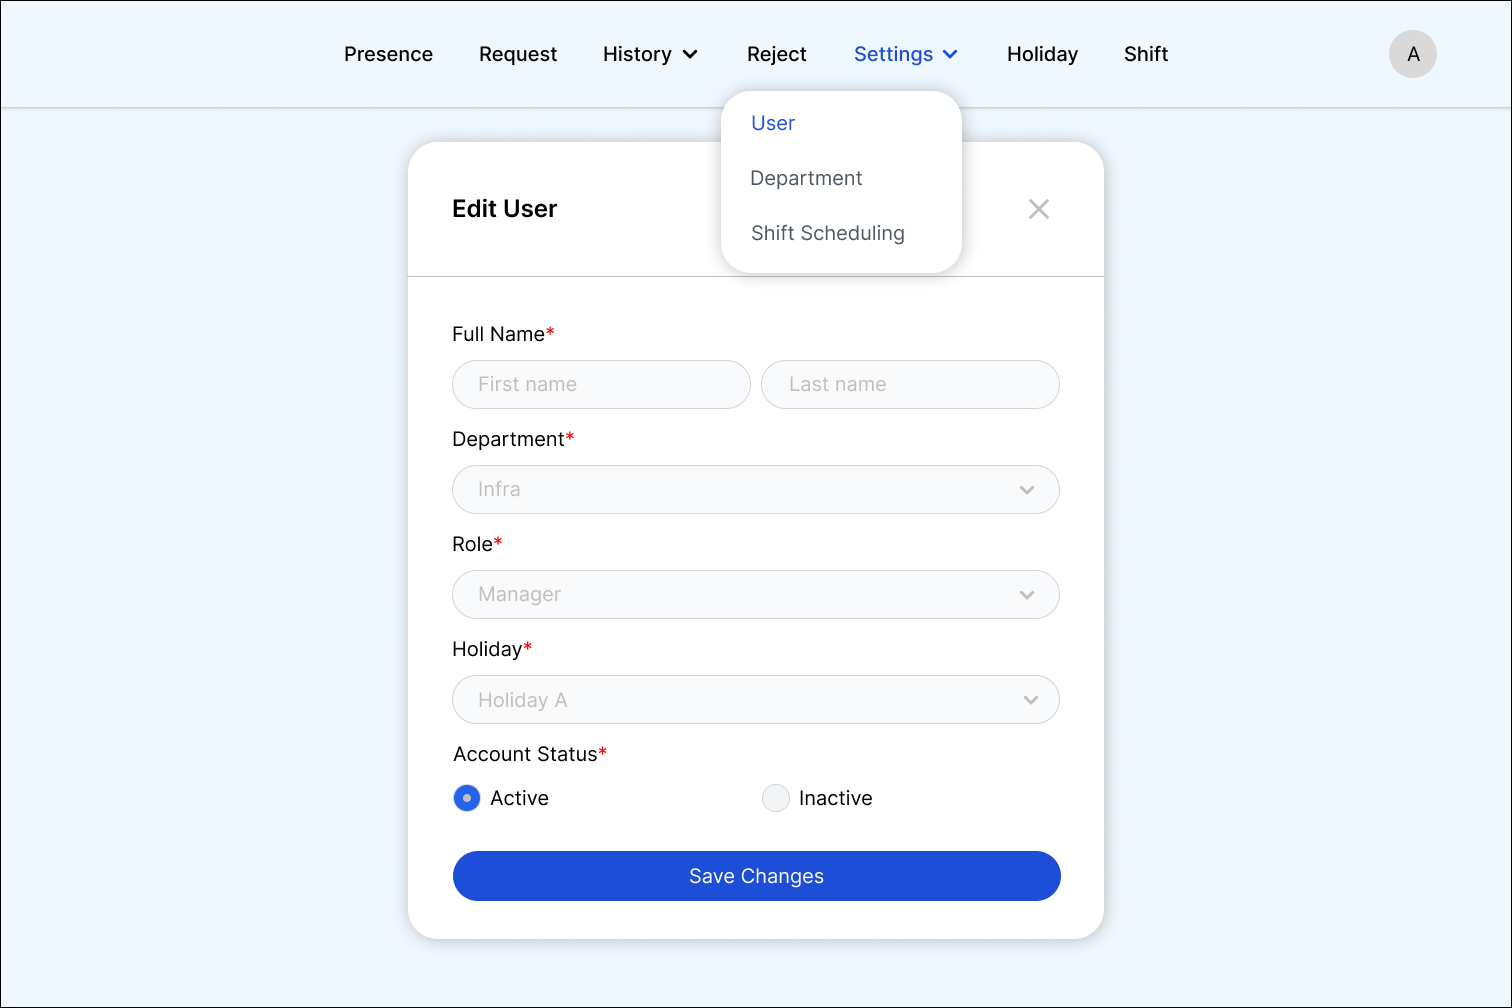
\includegraphics[width=13cm]{Gambar/bab2/mockups/menu-edit-user.png}
	\caption{\textit{Mockup} Menu \textit{Edit User}}
	\label{fig:mockup-menu-edit-user}
\end{figure}
\FloatBarrier

\begin{figure}[H]
	\centering
	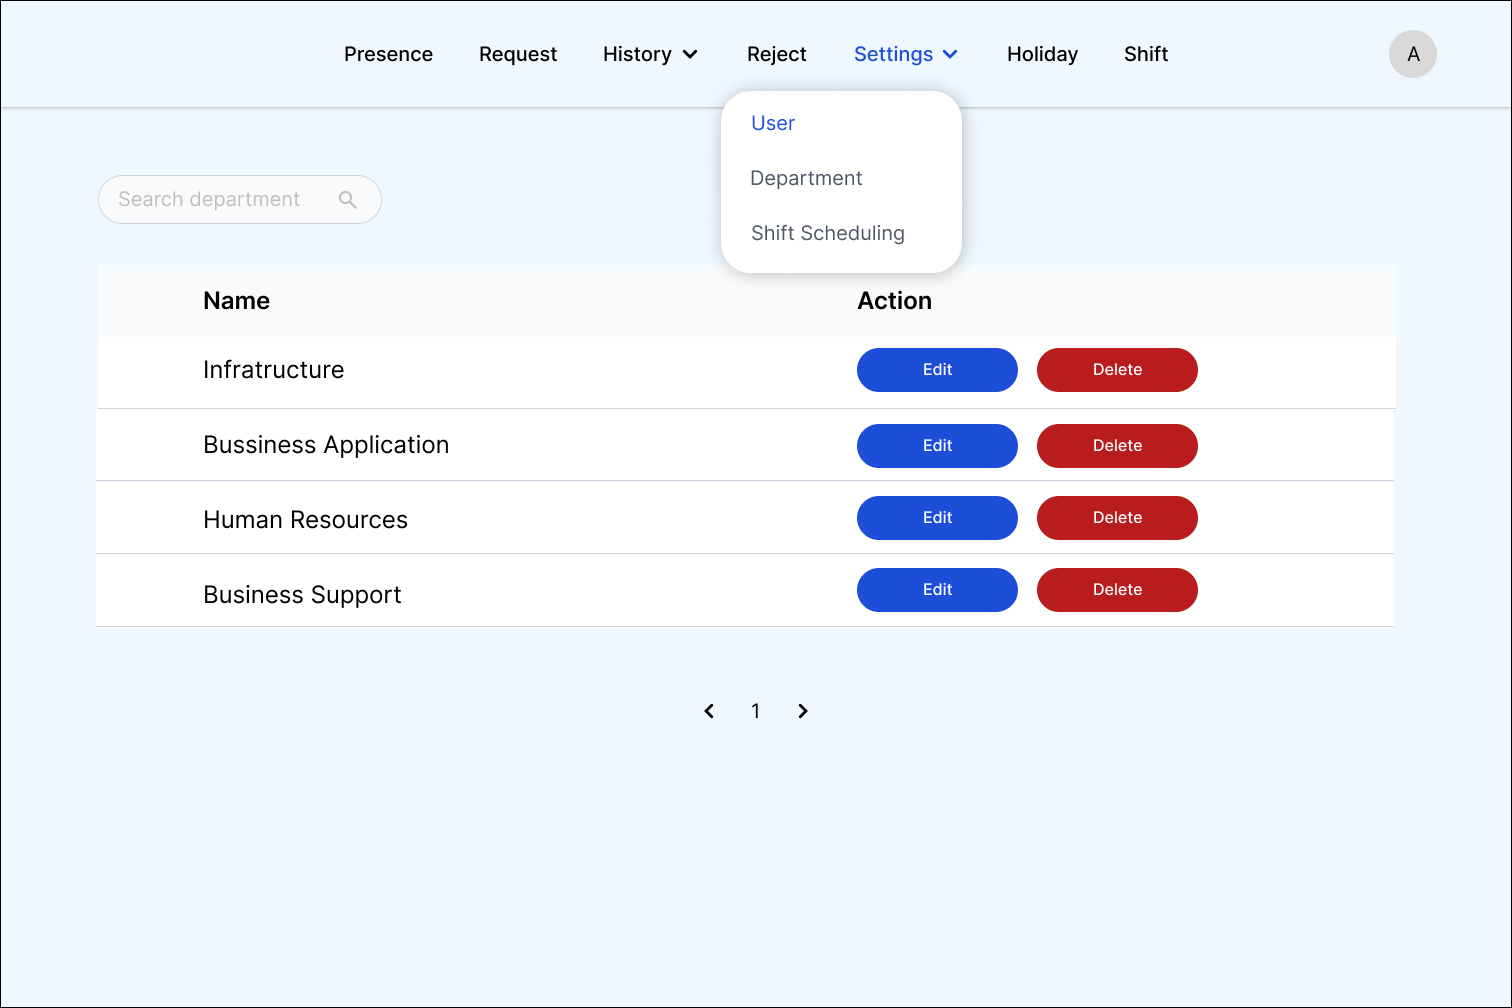
\includegraphics[width=13cm]{Gambar/bab2/mockups/menu-department.png}
	\caption{\textit{Mockup} Menu \textit{Department}}
	\label{fig:mockup-menu-department}
\end{figure}
\FloatBarrier

\begin{figure}[H]
	\centering
	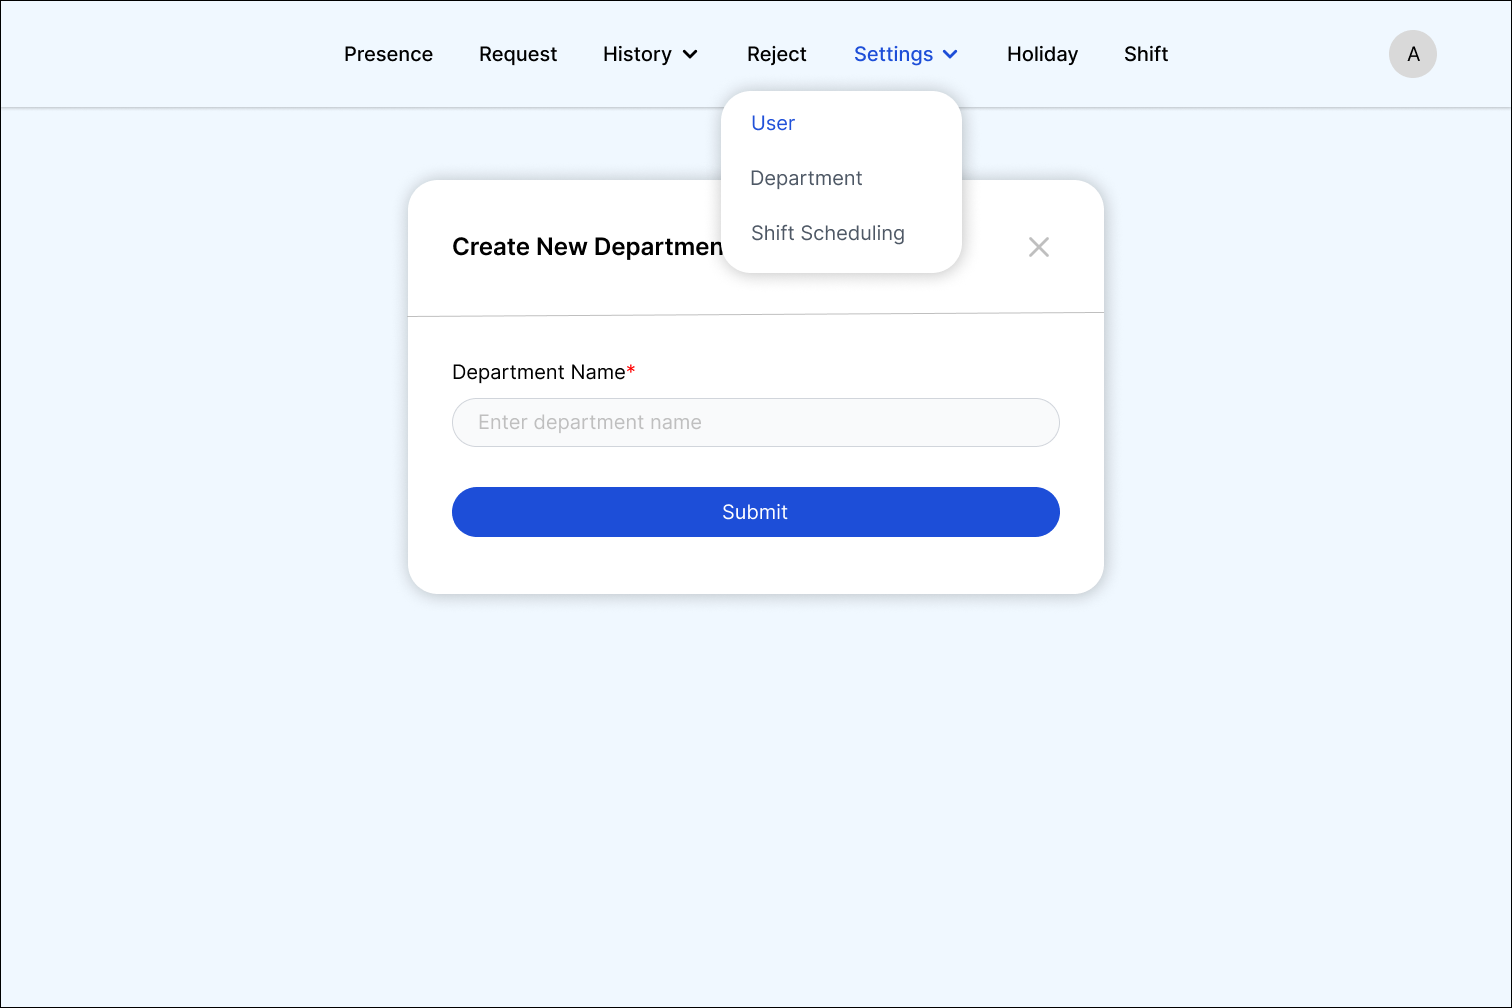
\includegraphics[width=13cm]{Gambar/bab2/mockups/menu-tambah-department.png}
	\caption{\textit{Mockup} Menu Tambah \textit{Department}}
	\label{fig:mockup-menu-tambah-department}
\end{figure}
\FloatBarrier

\begin{figure}[H]
	\centering
	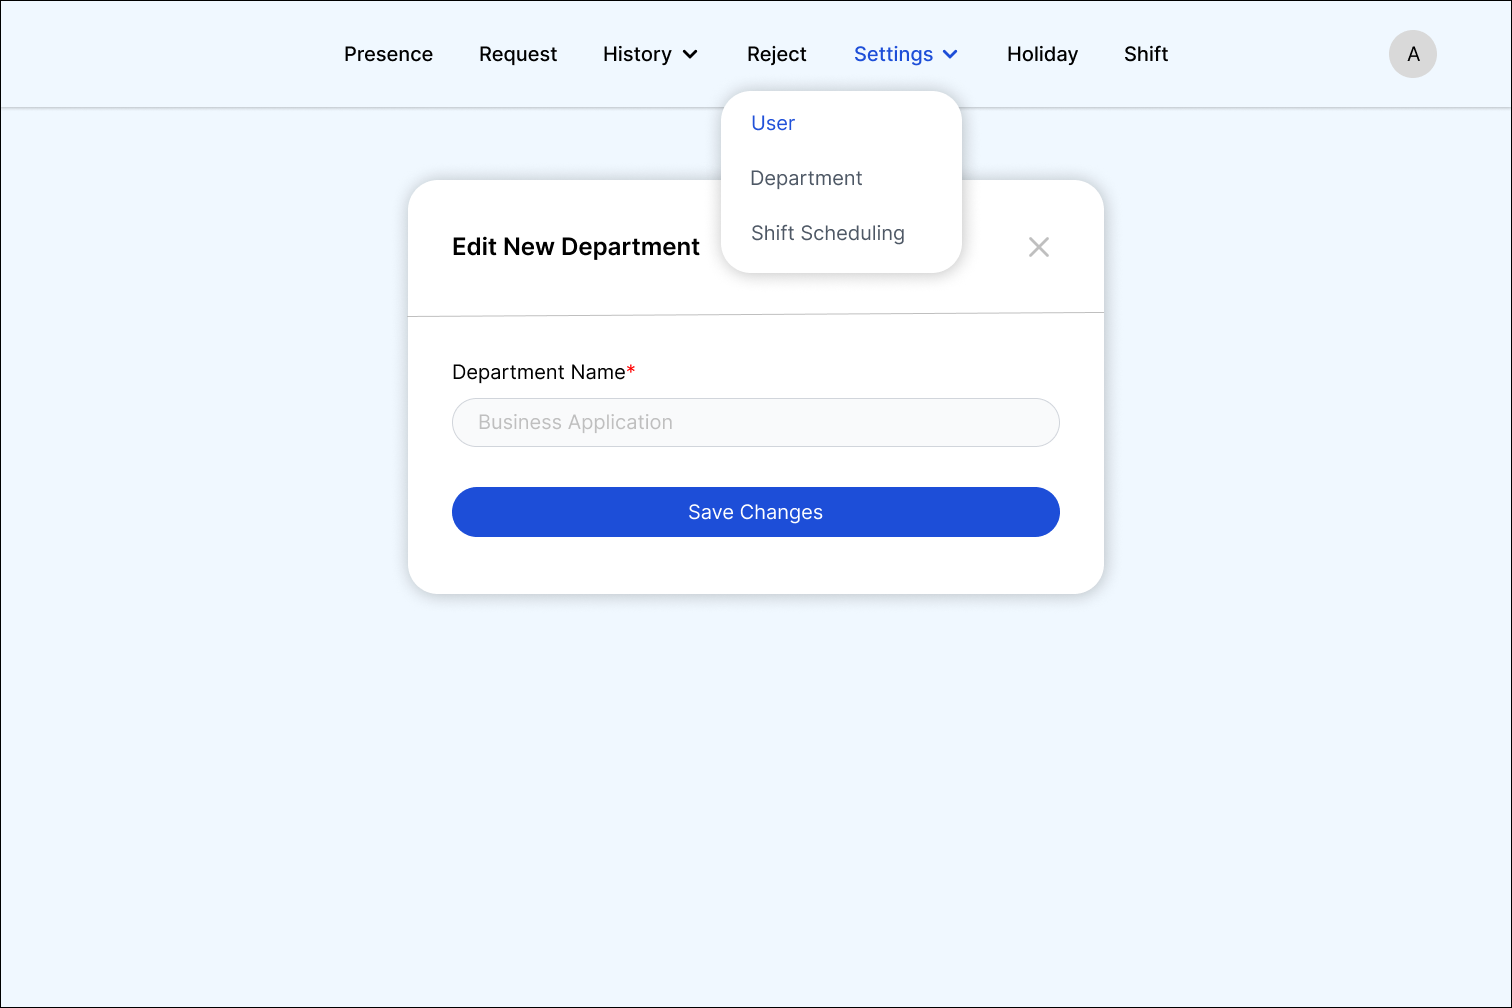
\includegraphics[width=13cm]{Gambar/bab2/mockups/menu-edit-department.png}
	\caption{\textit{Mockup} Menu \textit{Edit} \textit{Department}}
	\label{fig:mockup-menu-edit-department}
\end{figure}
\FloatBarrier

\begin{figure}[H]
	\centering
	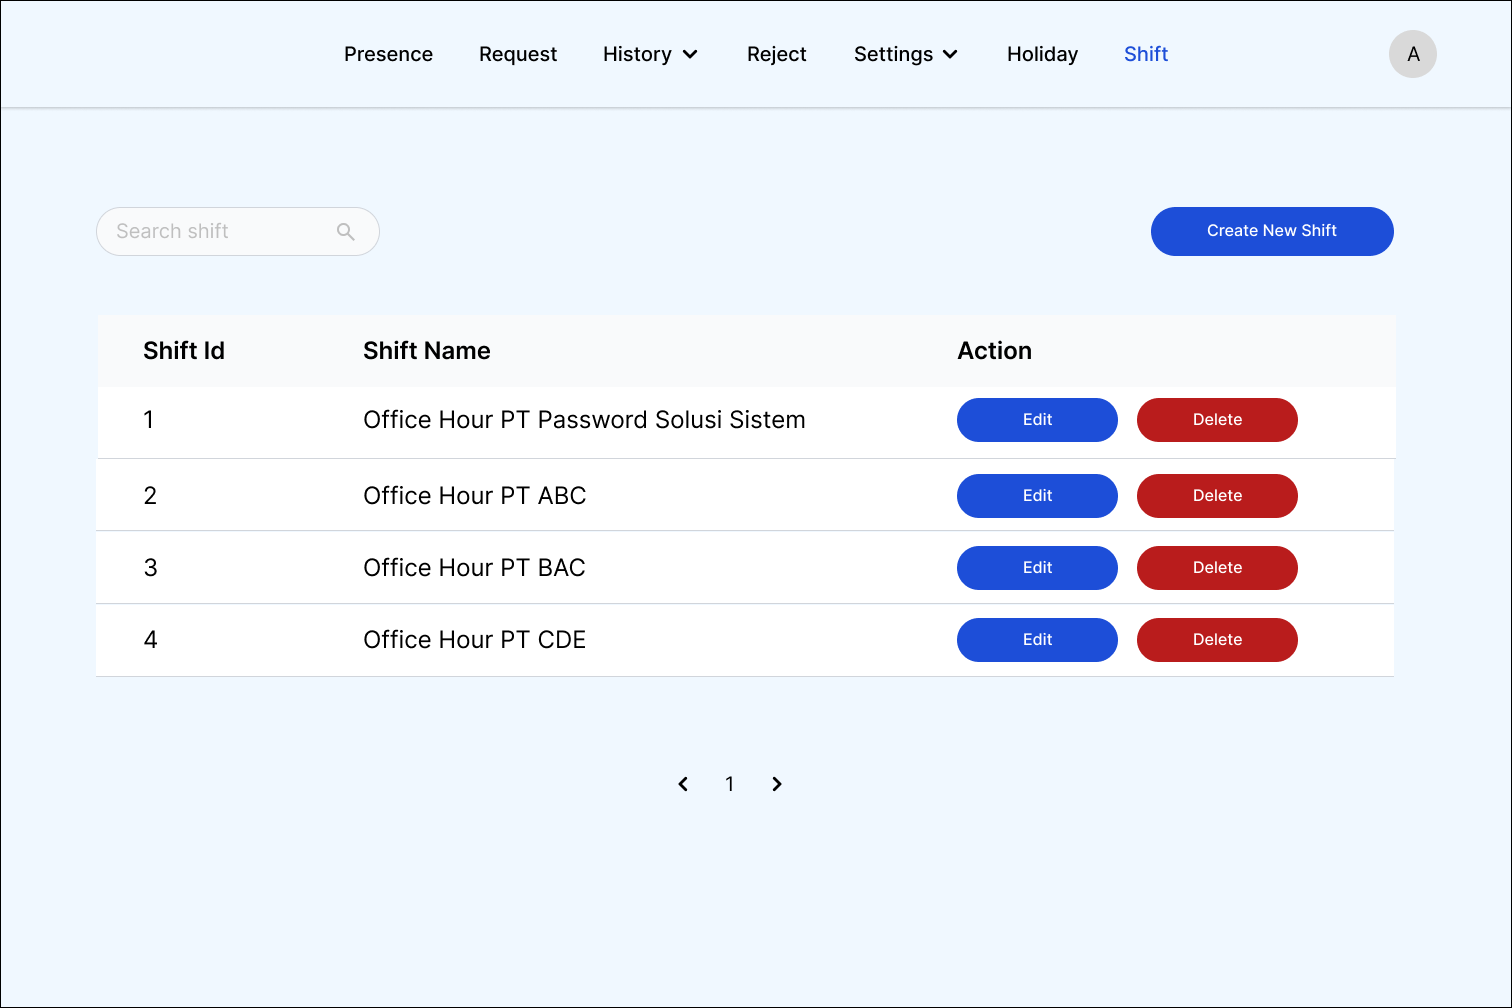
\includegraphics[width=13cm]{Gambar/bab2/mockups/menu-shift.png}
	\caption{\textit{Mockup} Menu \textit{Shift}}
	\label{fig:mockup-menu-shift}
\end{figure}
\FloatBarrier

\begin{figure}[H]
	\centering
	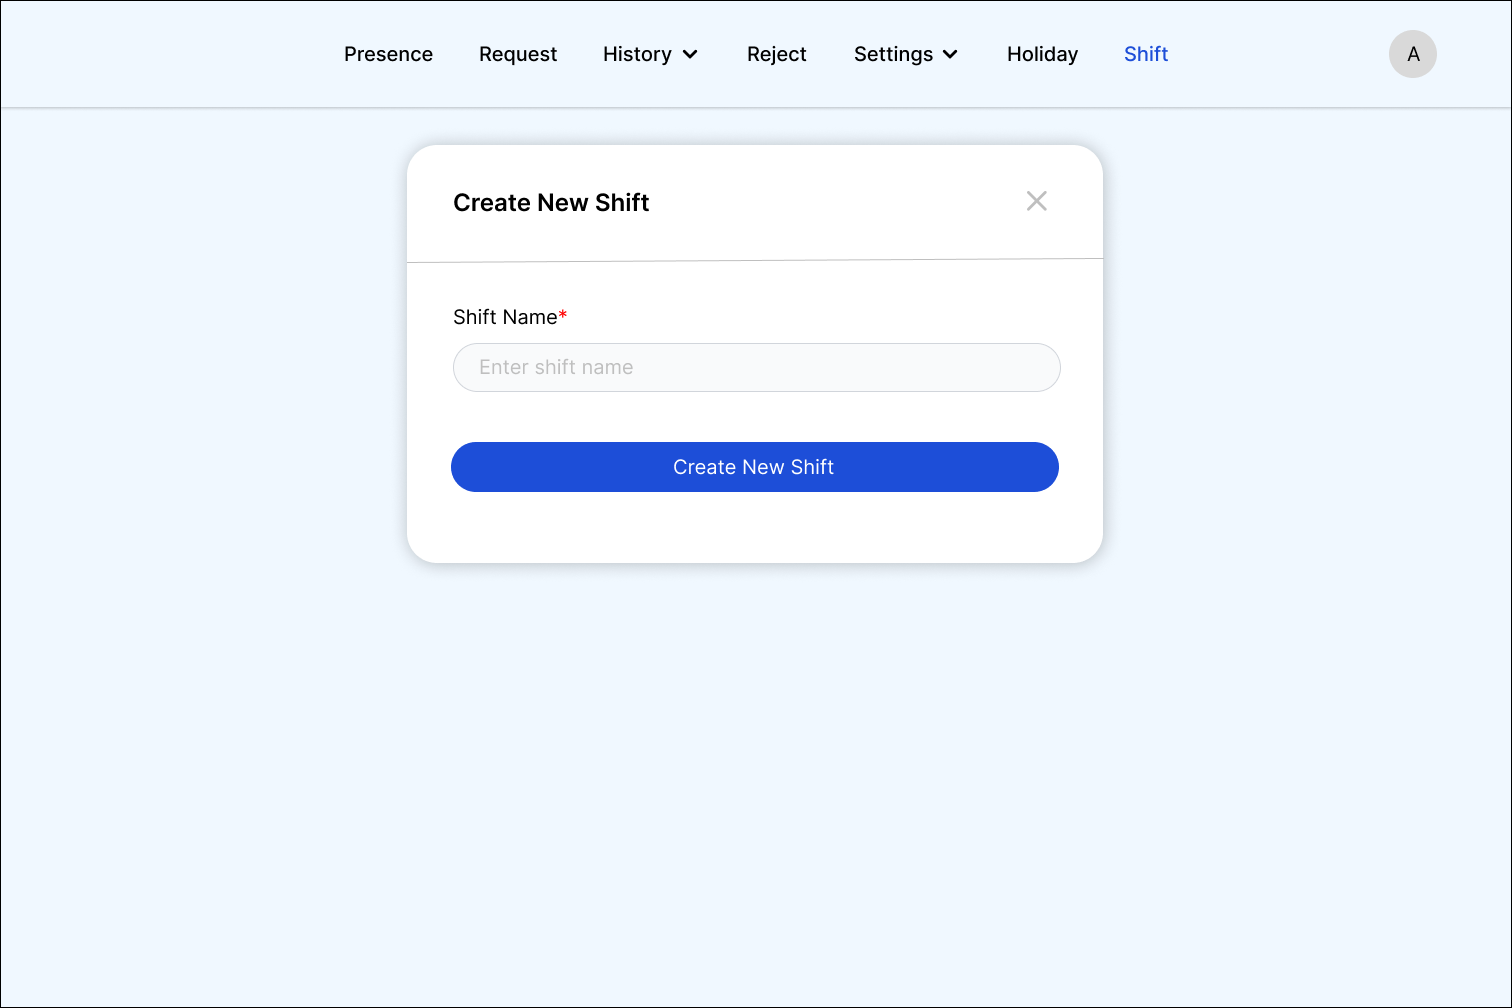
\includegraphics[width=13cm]{Gambar/bab2/mockups/menu-tambah-shift.png}
	\caption{\textit{Mockup} Menu Tambah \textit{Shift}}
	\label{fig:mockup-menu-tambah-shift}
\end{figure}
\FloatBarrier

\begin{figure}[H]
	\centering
	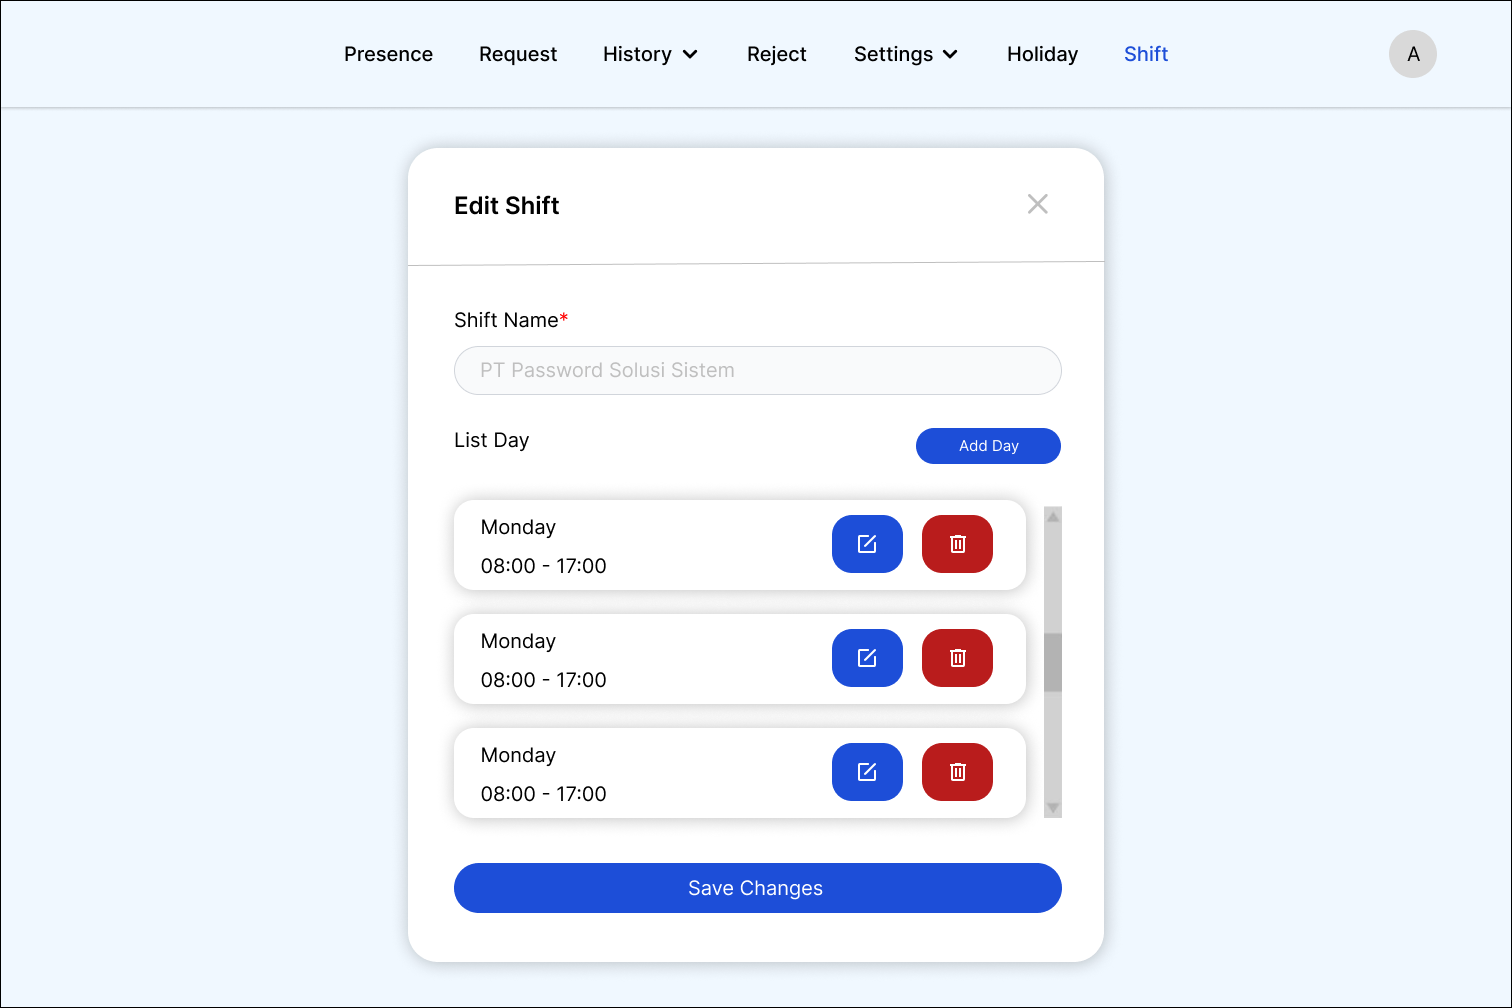
\includegraphics[width=13cm]{Gambar/bab2/mockups/menu-edit-shift.png}
	\caption{\textit{Mockup} Menu Hari \textit{Shift}}
	\label{fig:mockup-menu-edit-shift}
\end{figure}
\FloatBarrier

\begin{figure}[H]
	\centering
	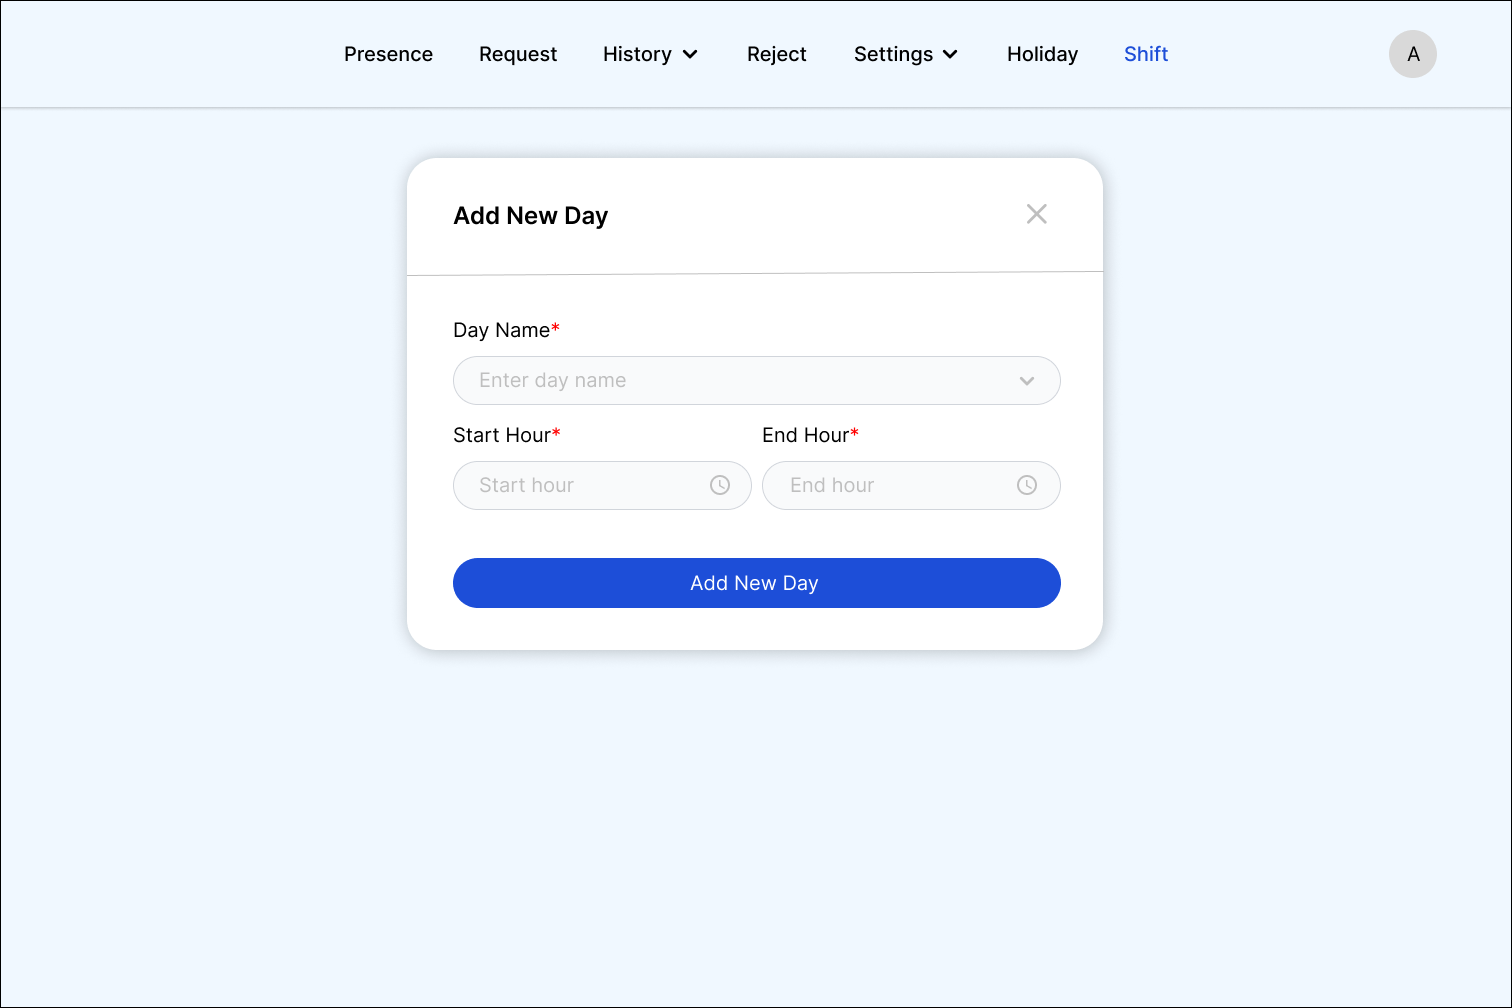
\includegraphics[width=13cm]{Gambar/bab2/mockups/menu-tambah-hari.png}
	\caption{\textit{Mockup} Menu Tambah Hari \textit{Shift}}
	\label{fig:mockup-menu-tambah-hari}
\end{figure}
\FloatBarrier

\begin{figure}[H]
	\centering
	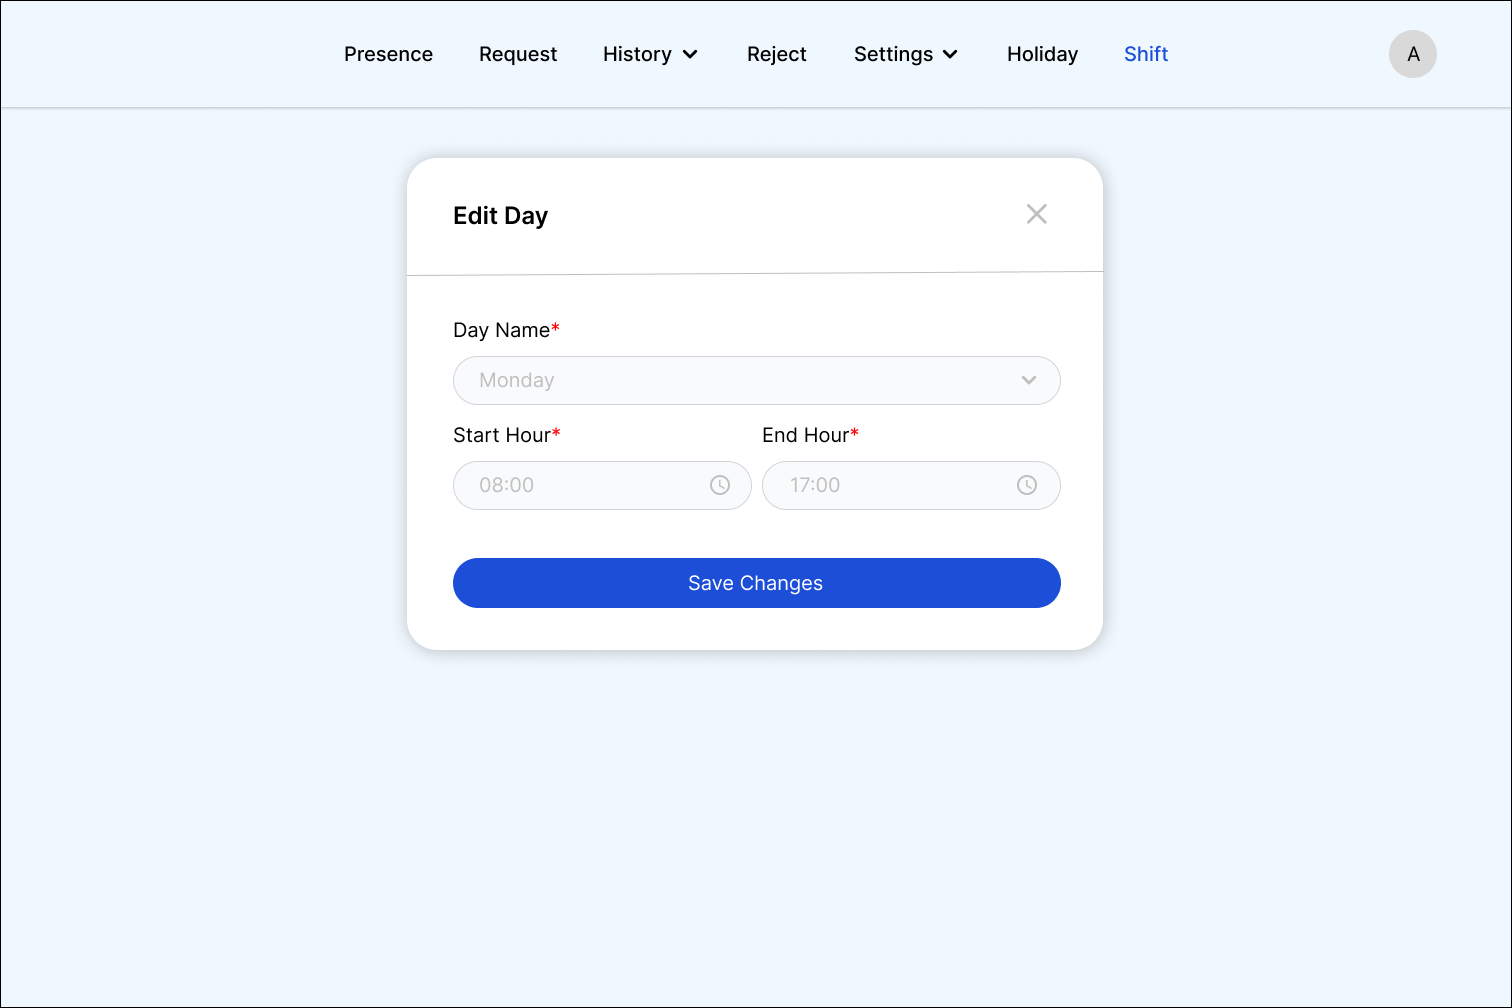
\includegraphics[width=13cm]{Gambar/bab2/mockups/menu-edit-hari.png}
	\caption{\textit{Mockup} Menu \textit{Edit} Hari \textit{Shift}}
	\label{fig:mockup-menu-edit-hari}
\end{figure}
\FloatBarrier

\begin{figure}[H]
	\centering
	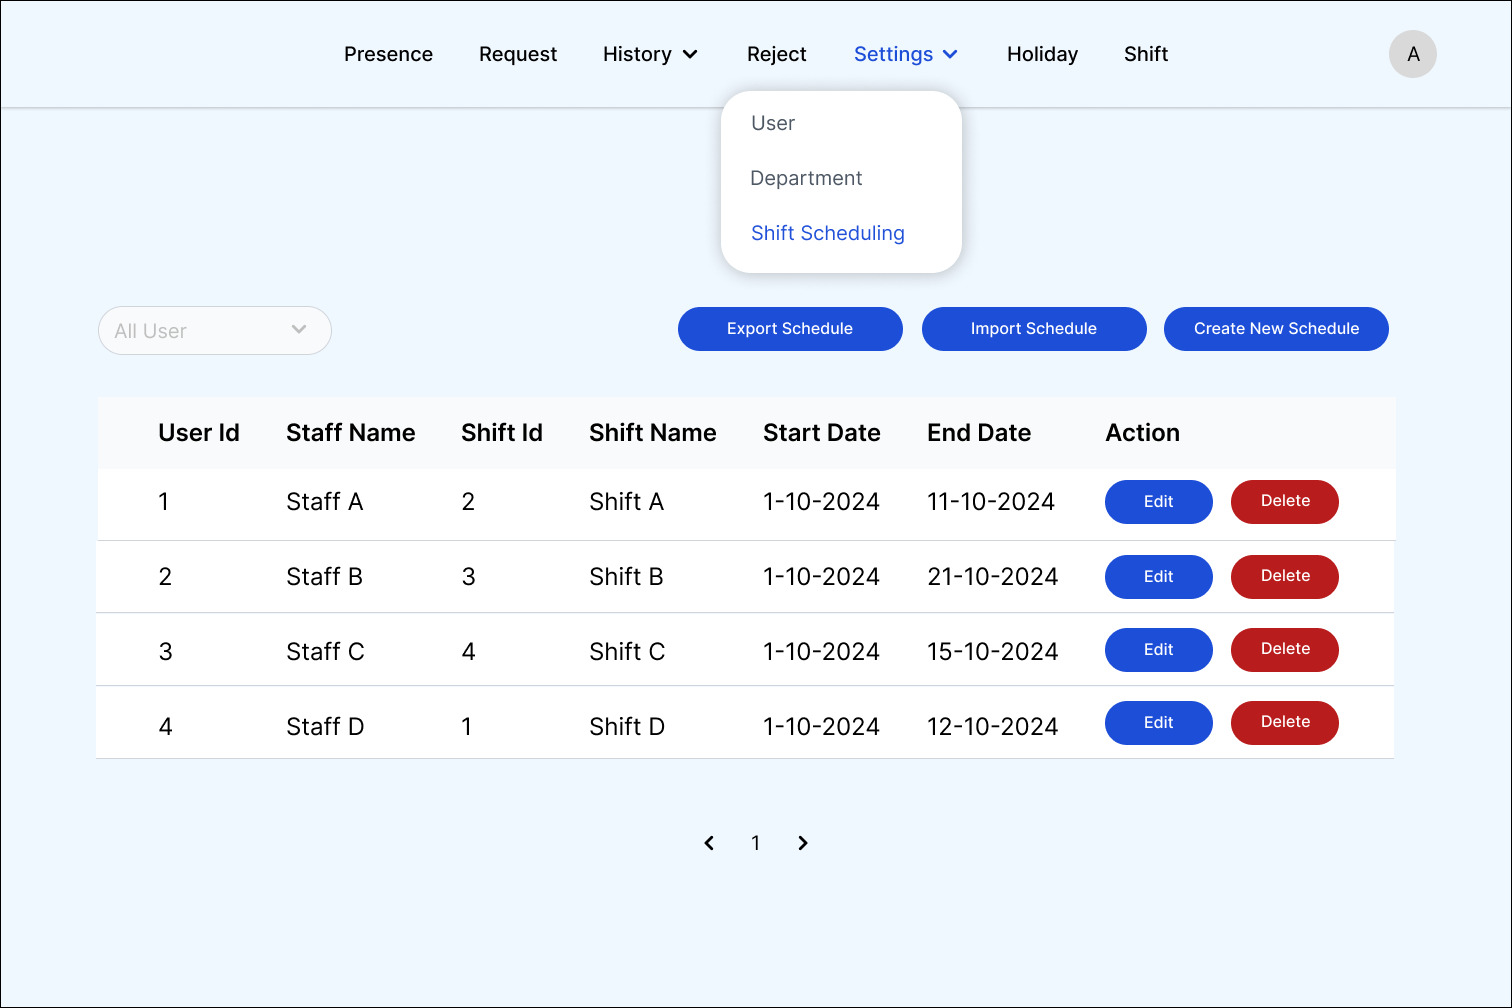
\includegraphics[width=13cm]{Gambar/bab2/mockups/menu-shift-scheduling.png}
	\caption{\textit{Mockup} Menu \textit{Shift Scheduling}}
	\label{fig:mockup-menu-scheduling-shift}
\end{figure}
\FloatBarrier

\begin{figure}[H]
	\centering
	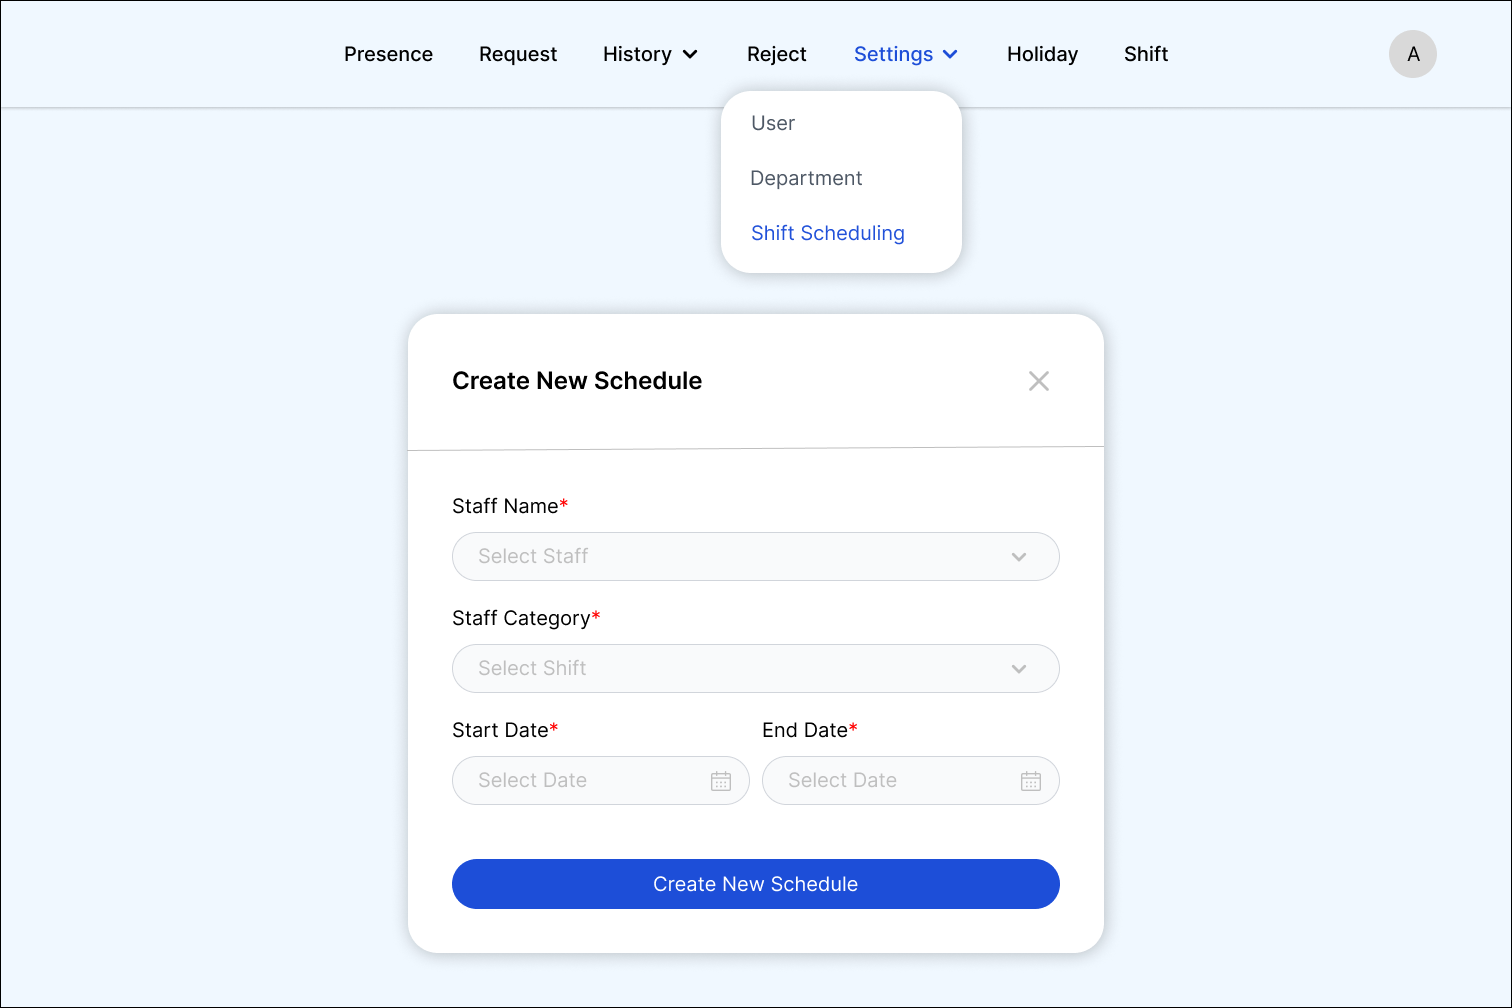
\includegraphics[width=13cm]{Gambar/bab2/mockups/menu-tambah-shift-scheduling.png}
	\caption{\textit{Mockup} Menu Tambah \textit{Shift Scheduling}}
	\label{fig:mockup-menu-tambah-scheduling-shift}
\end{figure}
\FloatBarrier

\begin{figure}[H]
	\centering
	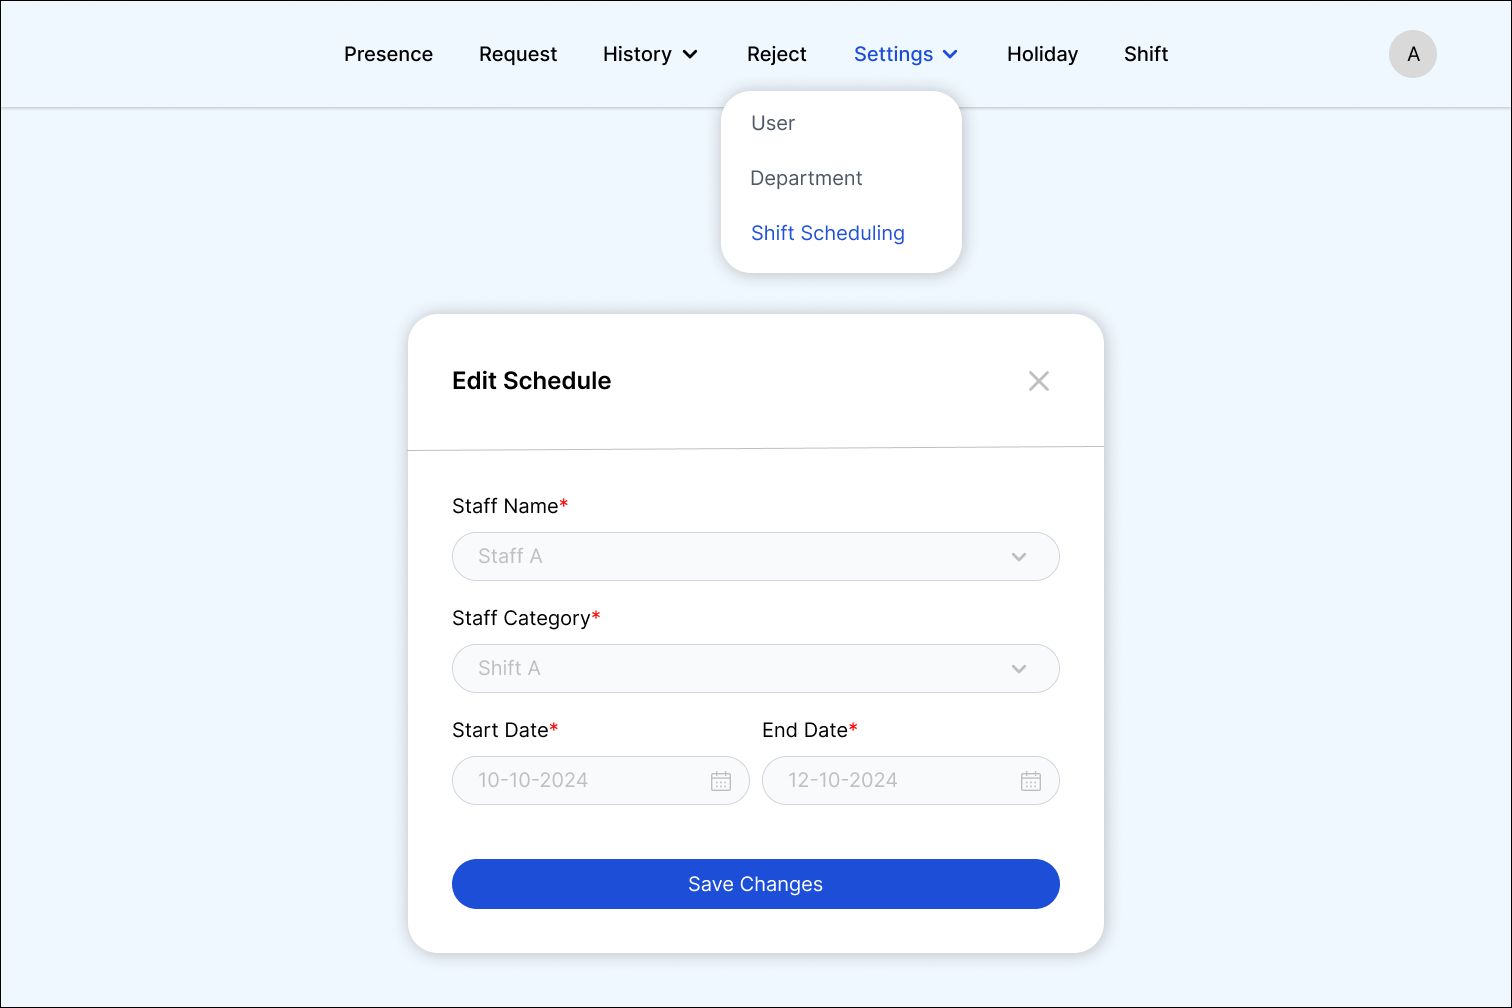
\includegraphics[width=13cm]{Gambar/bab2/mockups/menu-edit-shift-scheduling.png}
	\caption{\textit{Mockup} Menu \textit{Edit} \textit{Shift Scheduling}}
	\label{fig:mockup-menu-edit-scheduling-shift}
\end{figure}
\FloatBarrier

\begin{figure}[H]
	\centering
	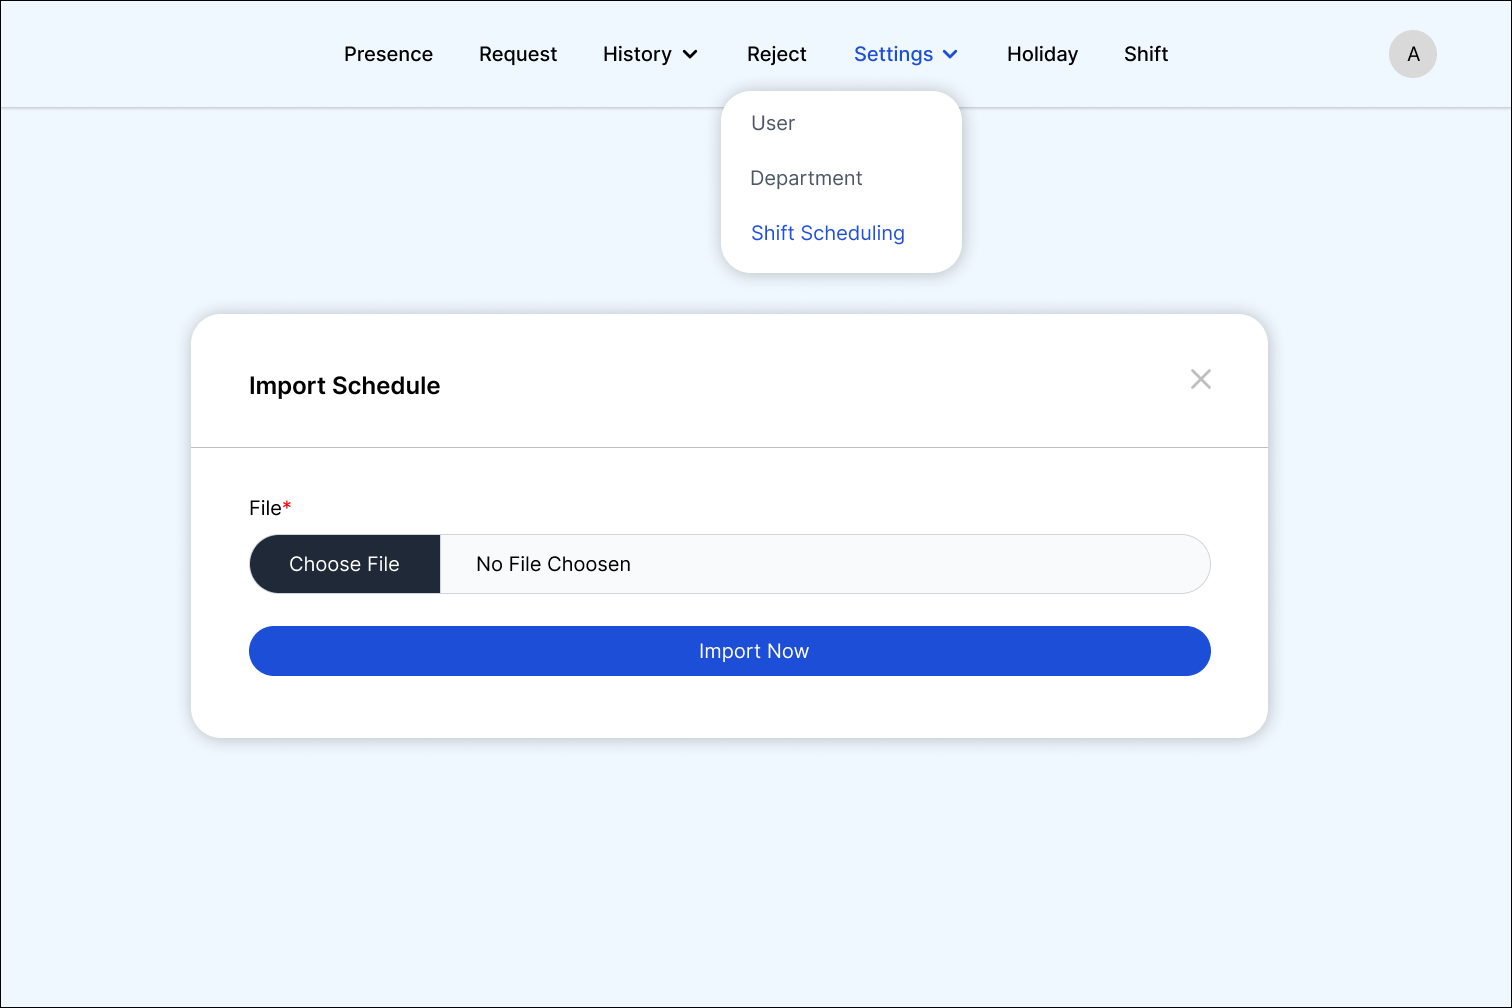
\includegraphics[width=13cm]{Gambar/bab2/mockups/menu-import-shift-scheduling.png}
	\caption{\textit{Mockup} Menu \textit{Import} \textit{Shift Scheduling}}
	\label{fig:mockup-menu-import-scheduling-shift}
\end{figure}
\FloatBarrier
\pagebreak

\nextappendix
\section*{Lampiran \theappendixletter: \textit{User Manual} Aplikasi Presensi \textit{Online}
\label{sec:user-manual-aplikasi-presensi-online}}
\addcontentsline{toc}{section}{Lampiran \theappendixletter: \textit{User Manual} Aplikasi Presensi \textit{Online}} 
%%%%%%%%%%%%%%%
% \setcounter{figure}{0}
% \setcounter{page}{1}
% \pagenumbering{gobble}
%%%%%%%%%%%%%%%

\begin{enumerate}
    \item Mengakses Aplikasi\label{item:mengakses-aplikasi}
    \begin{enumerate}
        \item Membuka aplikasi \textit{browser}, kemudian memasukkan tautan URL aplikasi presensi \textit{online}. \textbf{\ref{fig:memasukkan-tautan-url-melalui-browser}} menunjukkan cara memasukkan tautan URL melalui \textit{browser}.
        \begin{figure}[!htbp]
    	\centering
    	
\includegraphics[width=10cm]{Gambar/bab3/user-manual/user-manual-enter-link.png}
    	\caption{Memasukkan Tautan URL Melalui \textit{Browser}}
    	\label{fig:memasukkan-tautan-url-melalui-browser}
        \end{figure}
        \FloatBarrier

        \item Setelah memasukkan tautan URL, maka halaman akan otomatis teralihkan ke halaman \textit{login} pada aplikasi presensi \textit{online}. \textbf{\ref{fig:user-manual-halaman-login}} menunjukkan tampilan \textit{login} pada aplikasi presensi \textit{online}.
        \begin{figure}[!htbp]
    	\centering
    	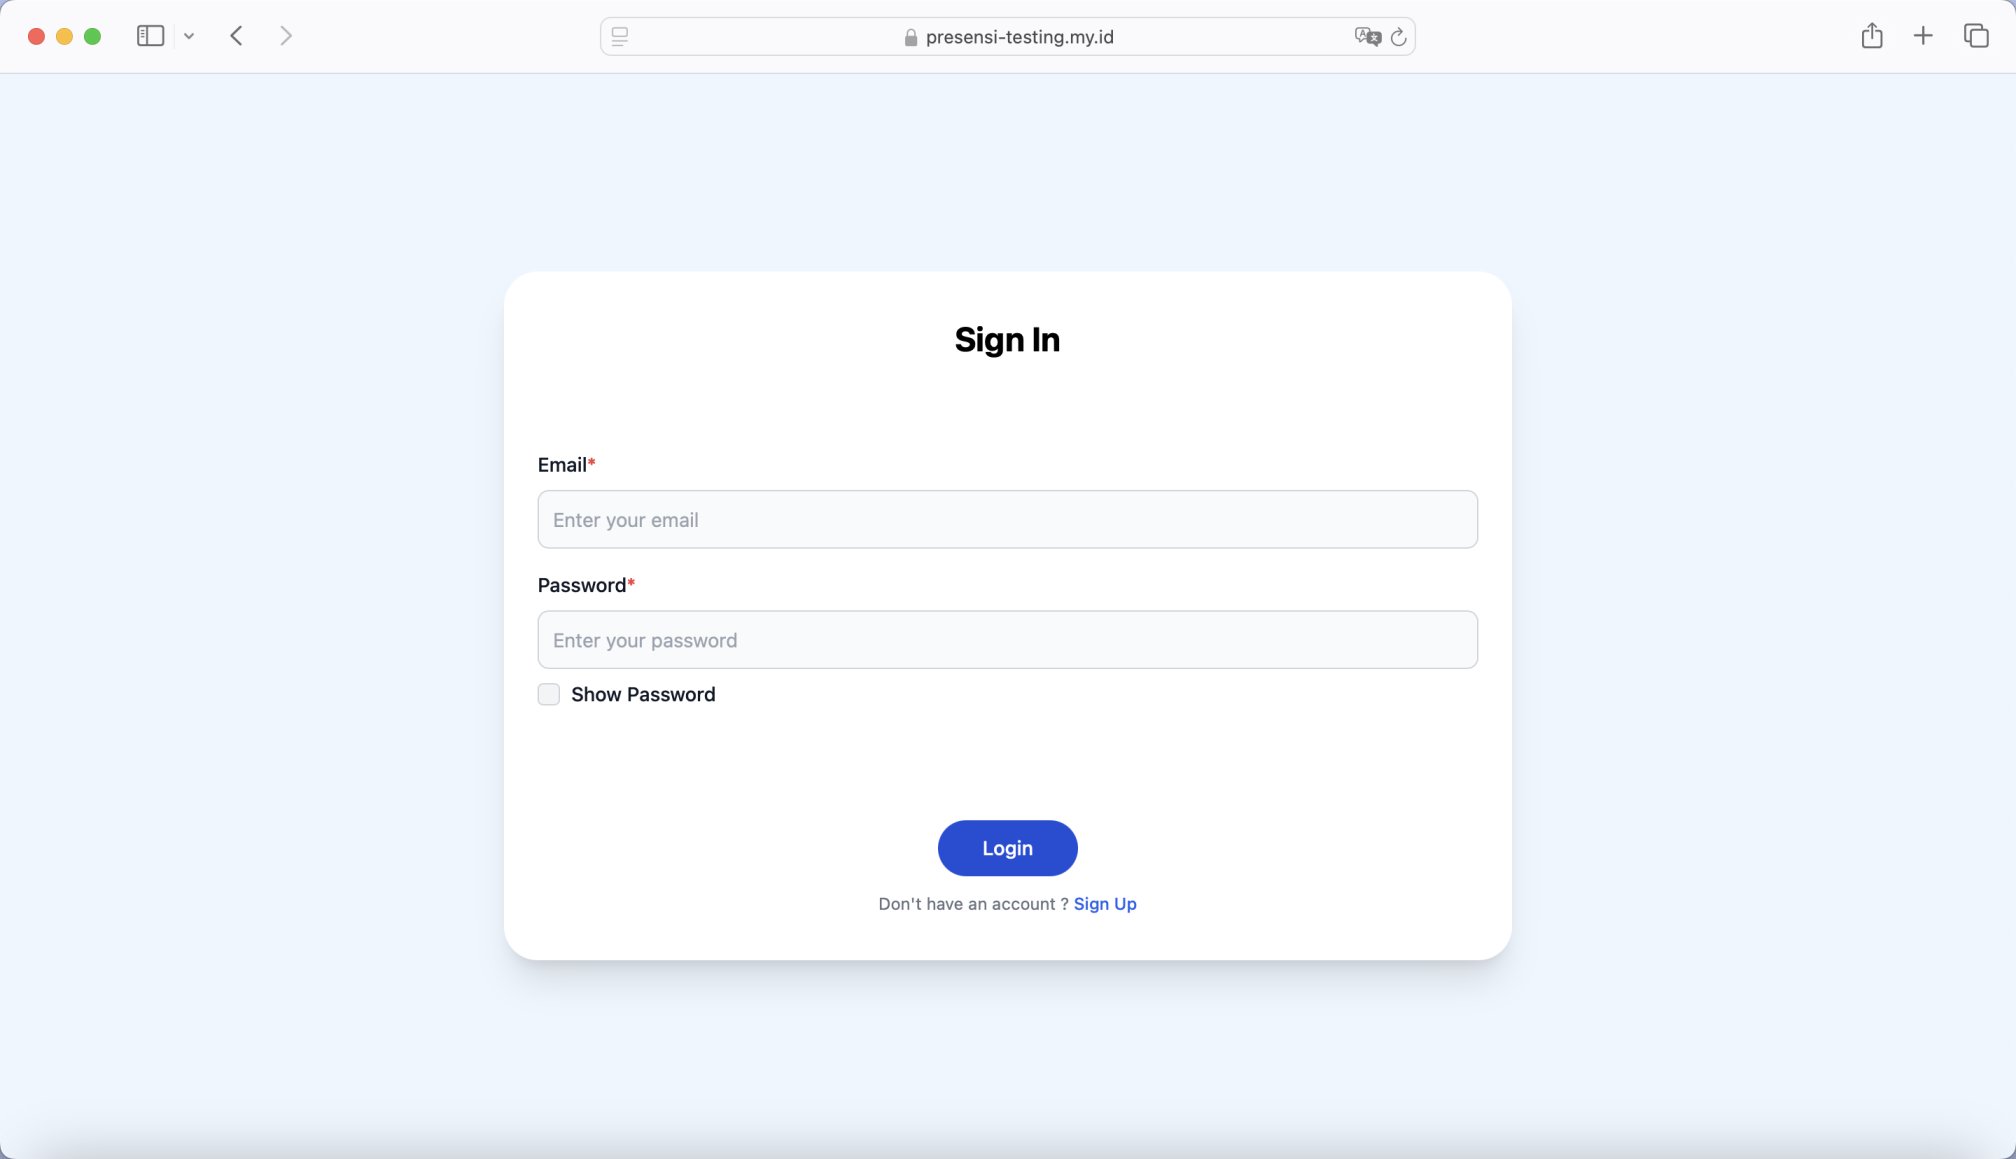
\includegraphics[width=10cm]{Gambar/bab3/user-manual/user-manual-halaman-login.png}
    	\caption{Tampilan Halaman \textit{Login}}
    	\label{fig:user-manual-halaman-login}
        \end{figure}
        \FloatBarrier
    \end{enumerate}

    \item Melakukan \textit{Login}\label{item:melakukan-login}
    \begin{enumerate}
        \item Mengakses aplikasi presensi \textit{online} yang terdapat pada \textbf{Manual \ref{item:mengakses-aplikasi}}.

        \item Mengisi seluruh \textit{input form} pada halaman \textit{login}, kemudian menekan tombol \textit{"Login"}. \textbf{\ref{fig:user-manual-halaman-login}} menunjukkan tampilan halaman \textit{login}.

        \item Halaman akan dialihkan ke halaman utama jika berhasil \textit{login}. \textbf{\ref{fig:user-manual-halaman-utama}} menunjukkan tampilan halaman utama aplikasi presensi \textit{online} ketika berhasil \textit{login}.

        \begin{figure}[!htbp]
    	\centering
    	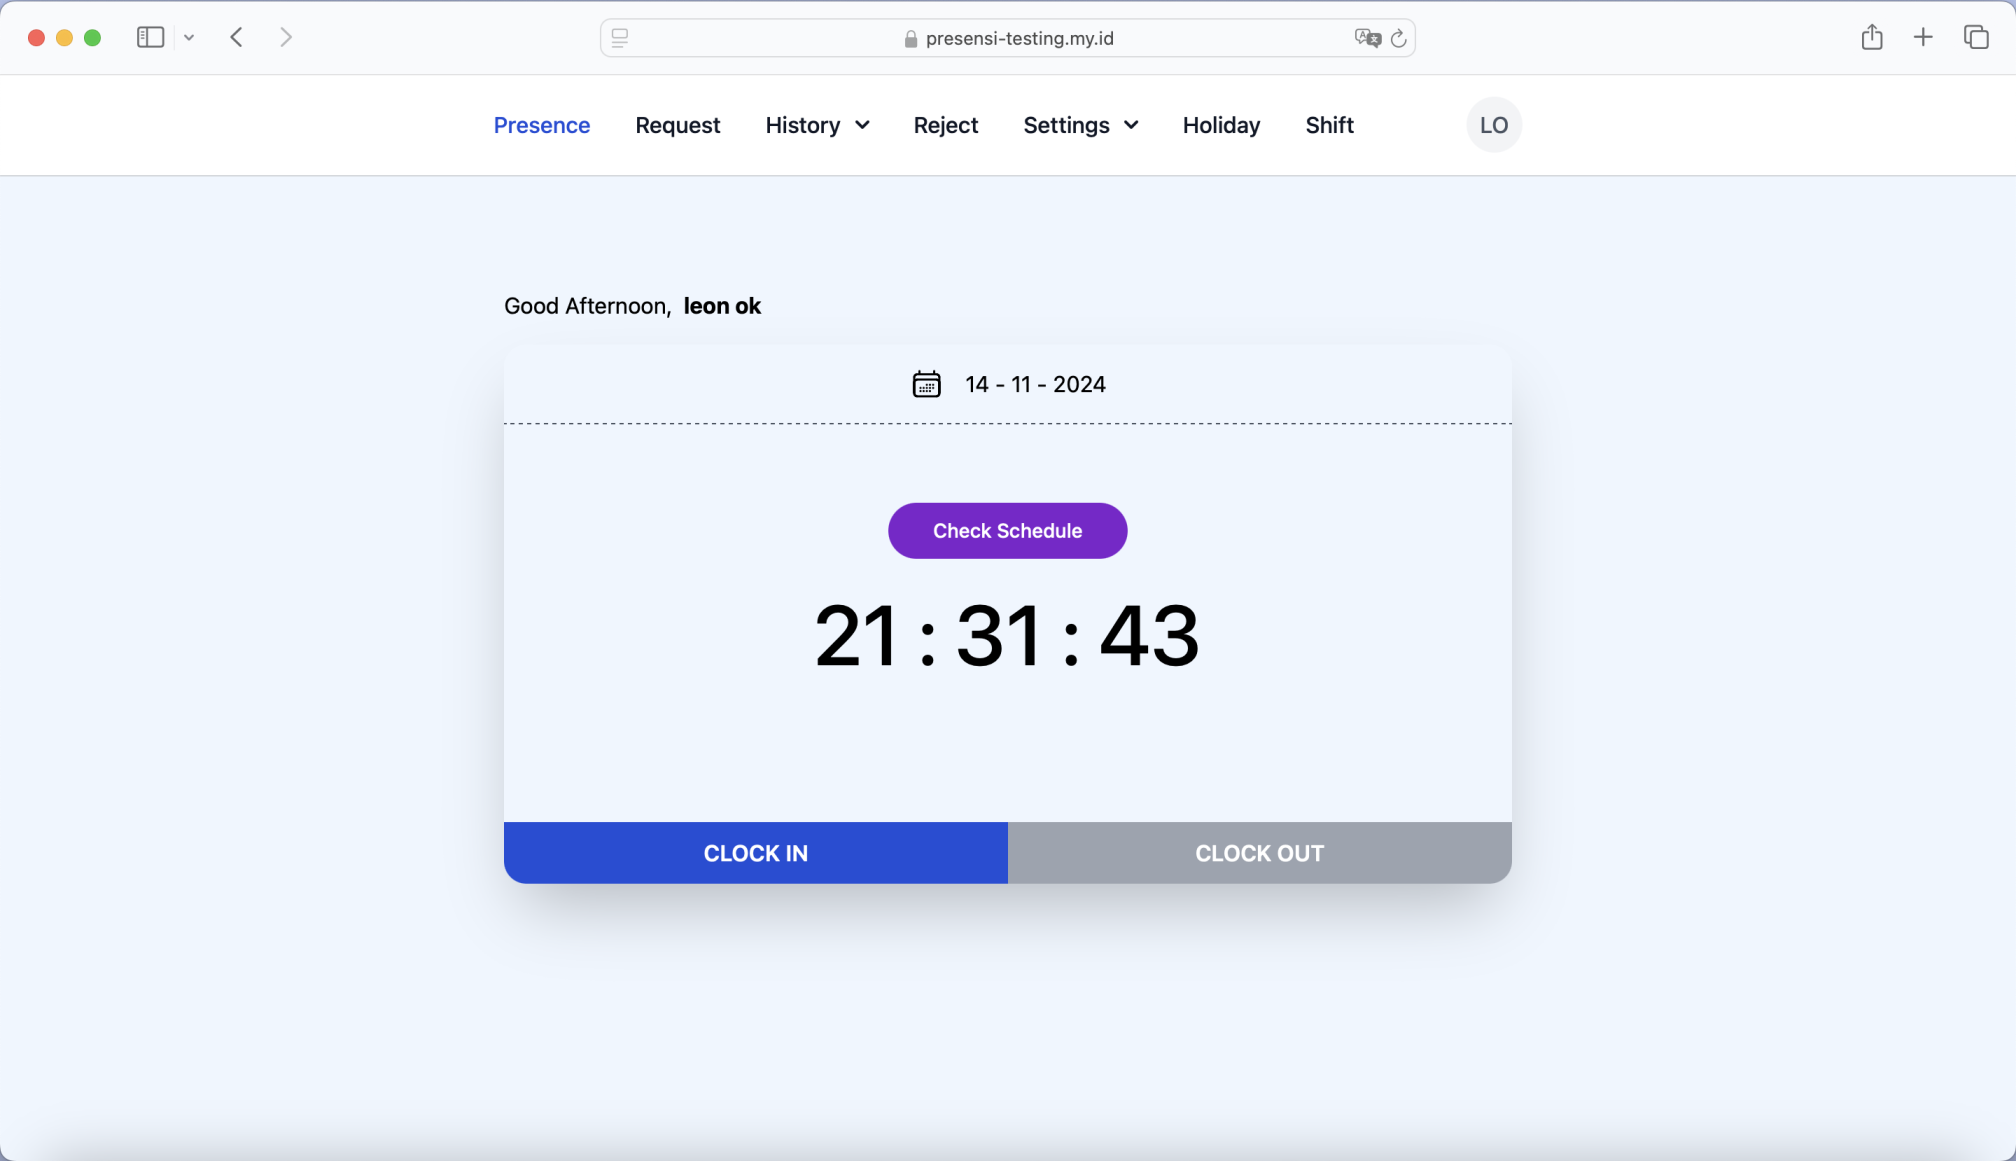
\includegraphics[width=10cm]{Gambar/bab3/user-manual/user-manual-halaman-utama.png}
    	\caption{Halaman Utama}
    	\label{fig:user-manual-halaman-utama}
        \end{figure}
        \FloatBarrier
    \end{enumerate}

    \item Melakukan Registrasi Akun
    \begin{enumerate}
        \item Mengakses aplikasi presensi \textit{online} yang terdapat pada \textbf{Manual \ref{item:mengakses-aplikasi}}.
        \item Menekan tombol \textit{"Sign Up"} pada halaman \textit{login}. \textbf{\ref{fig:user-manual-tombol-sign-up}} terdapat tombol \textit{"Sign Up"} yang terletak di paling bawah halaman.
        \item Mengisi seluruh \textit{input form} yang ada pada halaman registrasi akun dan menekan tombol \textit{"Register"}. \textbf{\ref{fig:user-manual-halaman-sign-up}} menunjukkan halaman registrasi akun.
        \item Sistem akan mengirimkan 6 digit kode OTP ke \textit{email} pengguna, memasukkan kode OTP ke dalam modal verifikasi \textit{email}. \textbf{\ref{fig:user-manual-verifikasi-email}} menunjukkan modal untuk verifikasi \textit{email} pada akun.
        \item Setelah memasukkan kode verifikasi \textit{email} dengan benar maka akan muncul pesan berhasil. \textbf{\ref{fig:user-manual-pesan-berhasil-verifikasi}} menunjukkan \textit{pop up} pesan berhasil verifikasi \textit{email} pada akun.
        \begin{figure}[!htbp]
    	\centering
    	
\includegraphics[width=10cm]{Gambar/bab3/user-manual/user-manual-tombol-sign-up.png}
    	\caption{Tombol \textit{Sign Up} Pada Halaman \textit{Login}}
    	\label{fig:user-manual-tombol-sign-up}
        \end{figure}
        \FloatBarrier

        \begin{figure}[!htbp]
    	\centering
    	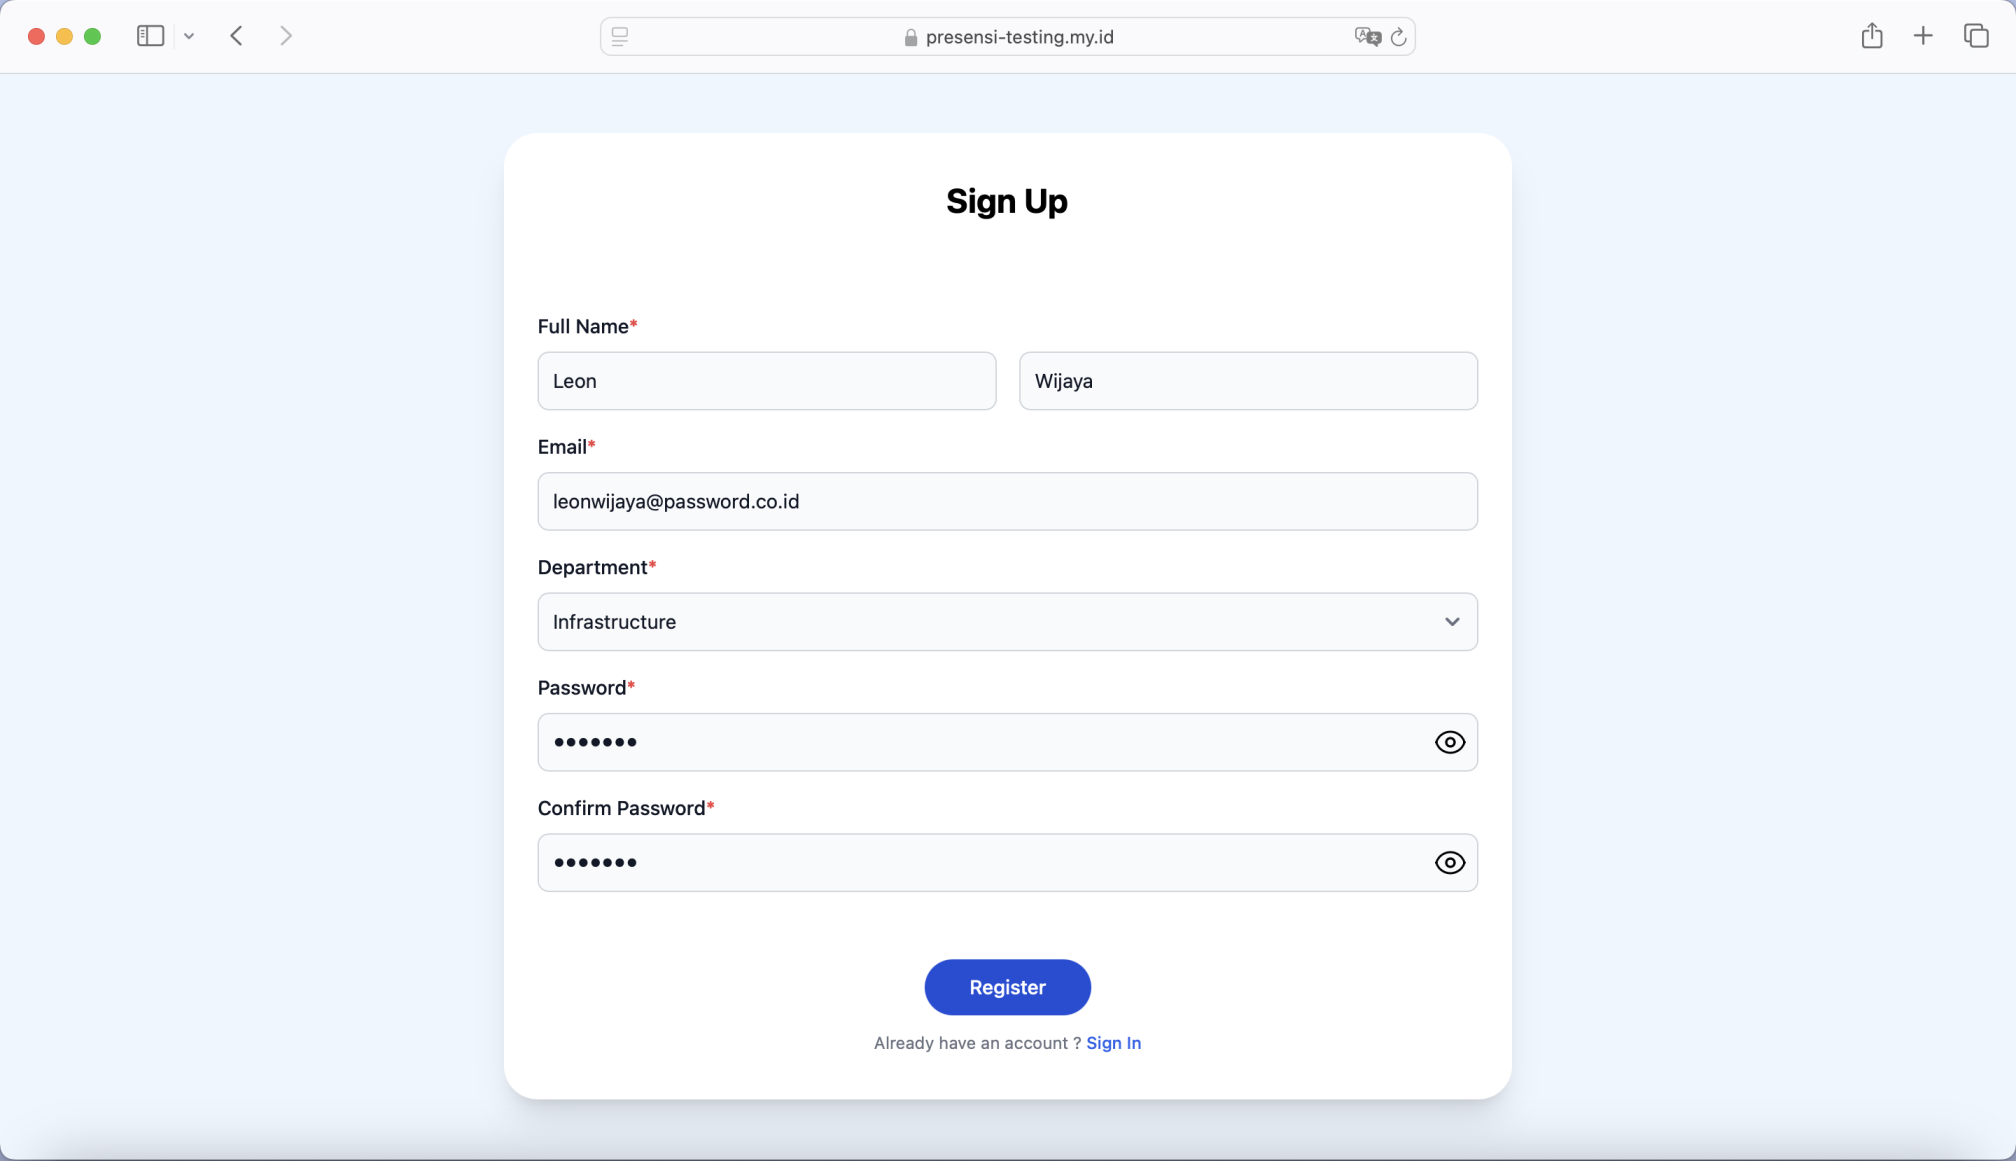
\includegraphics[width=10cm]{Gambar/bab3/user-manual/user-manual-halaman-sign-up.png}
    	\caption{Halaman Registrasi Akun}
    	\label{fig:user-manual-halaman-sign-up}
        \end{figure}
        \FloatBarrier

        \begin{figure}[!htbp]
    	\centering
    	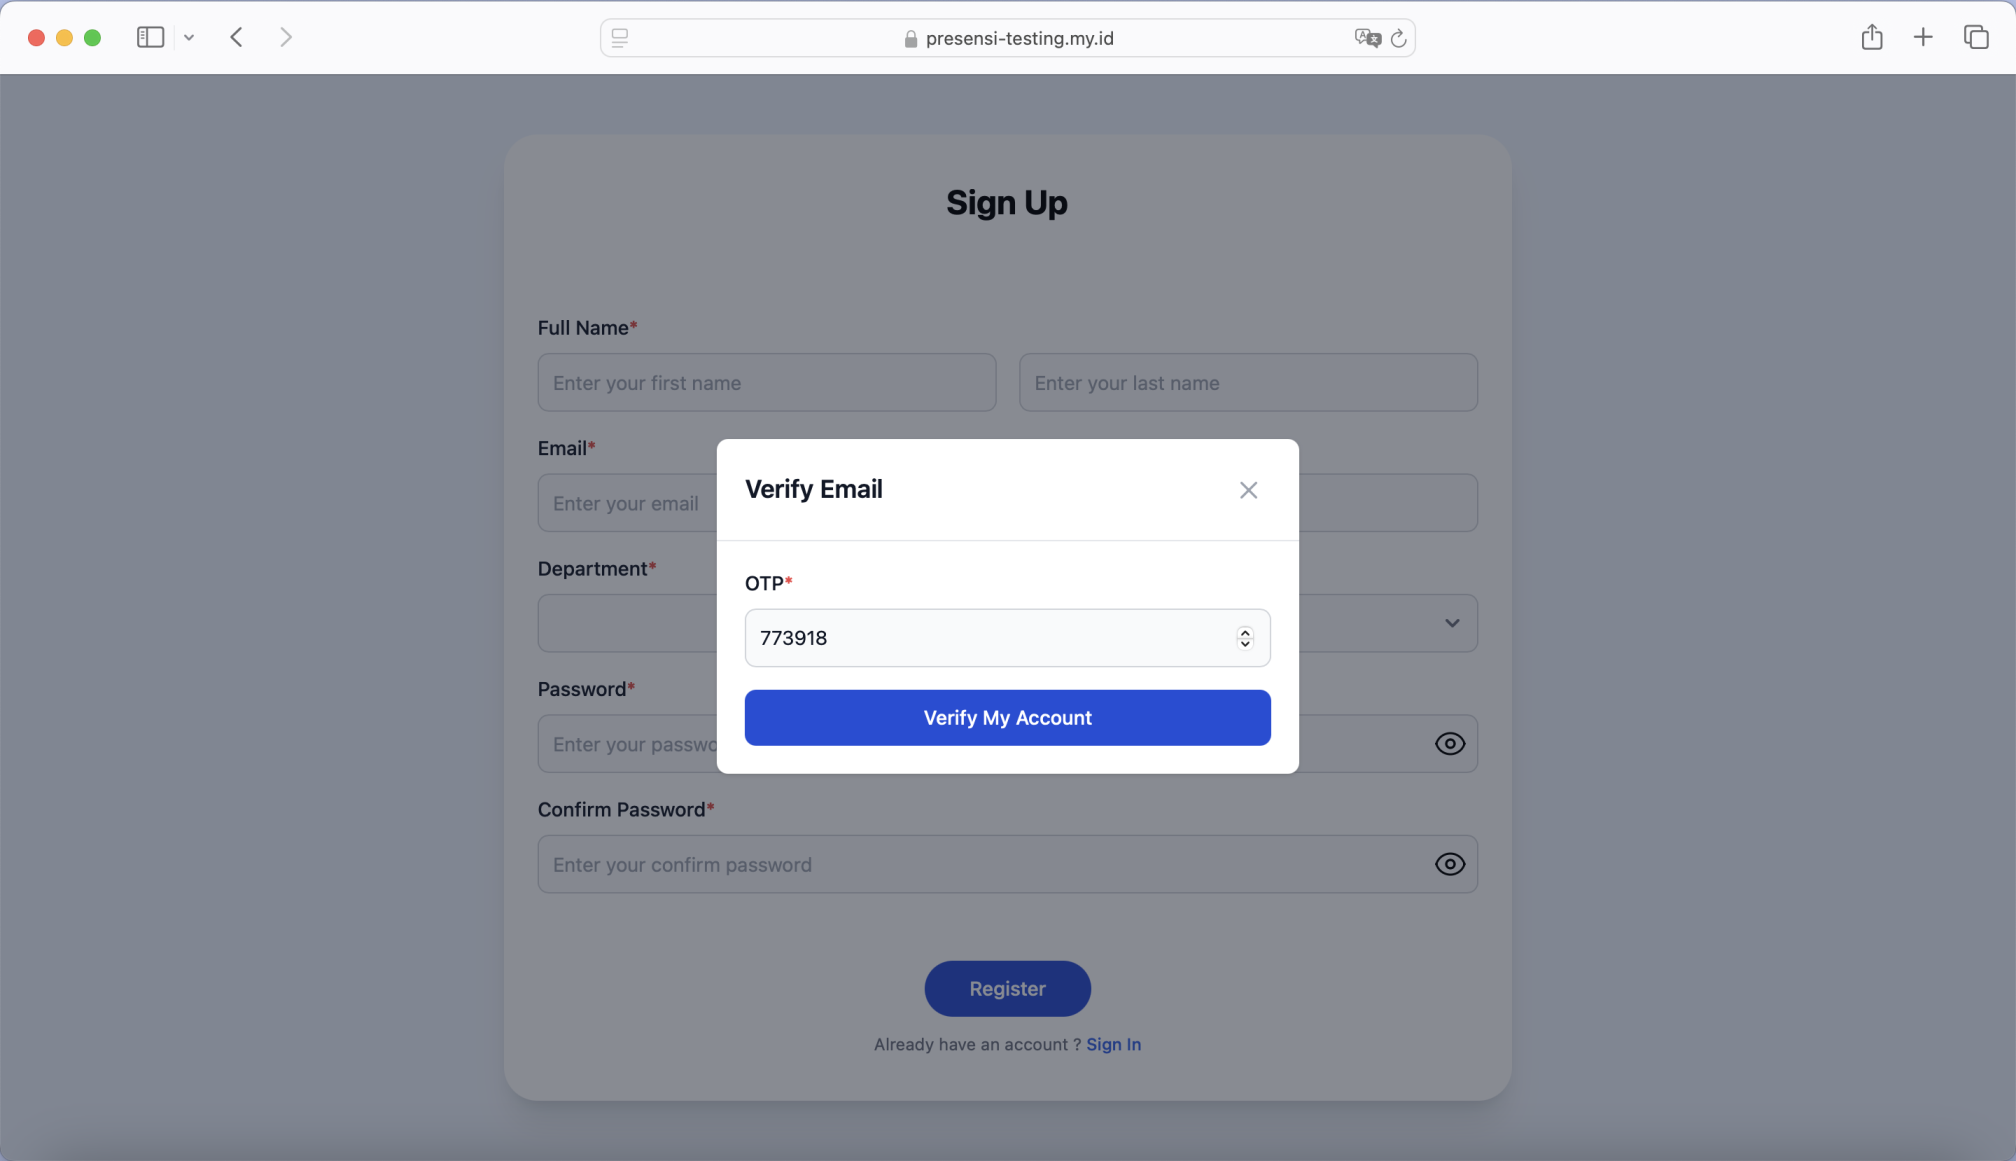
\includegraphics[width=10cm]{Gambar/bab3/user-manual/user-manual-verifikasi-email.png}
    	\caption{Modal Verifikasi \textit{Email}}
    	\label{fig:user-manual-verifikasi-email}
        \end{figure}
        \FloatBarrier

        \begin{figure}[!htbp]
    	\centering
    	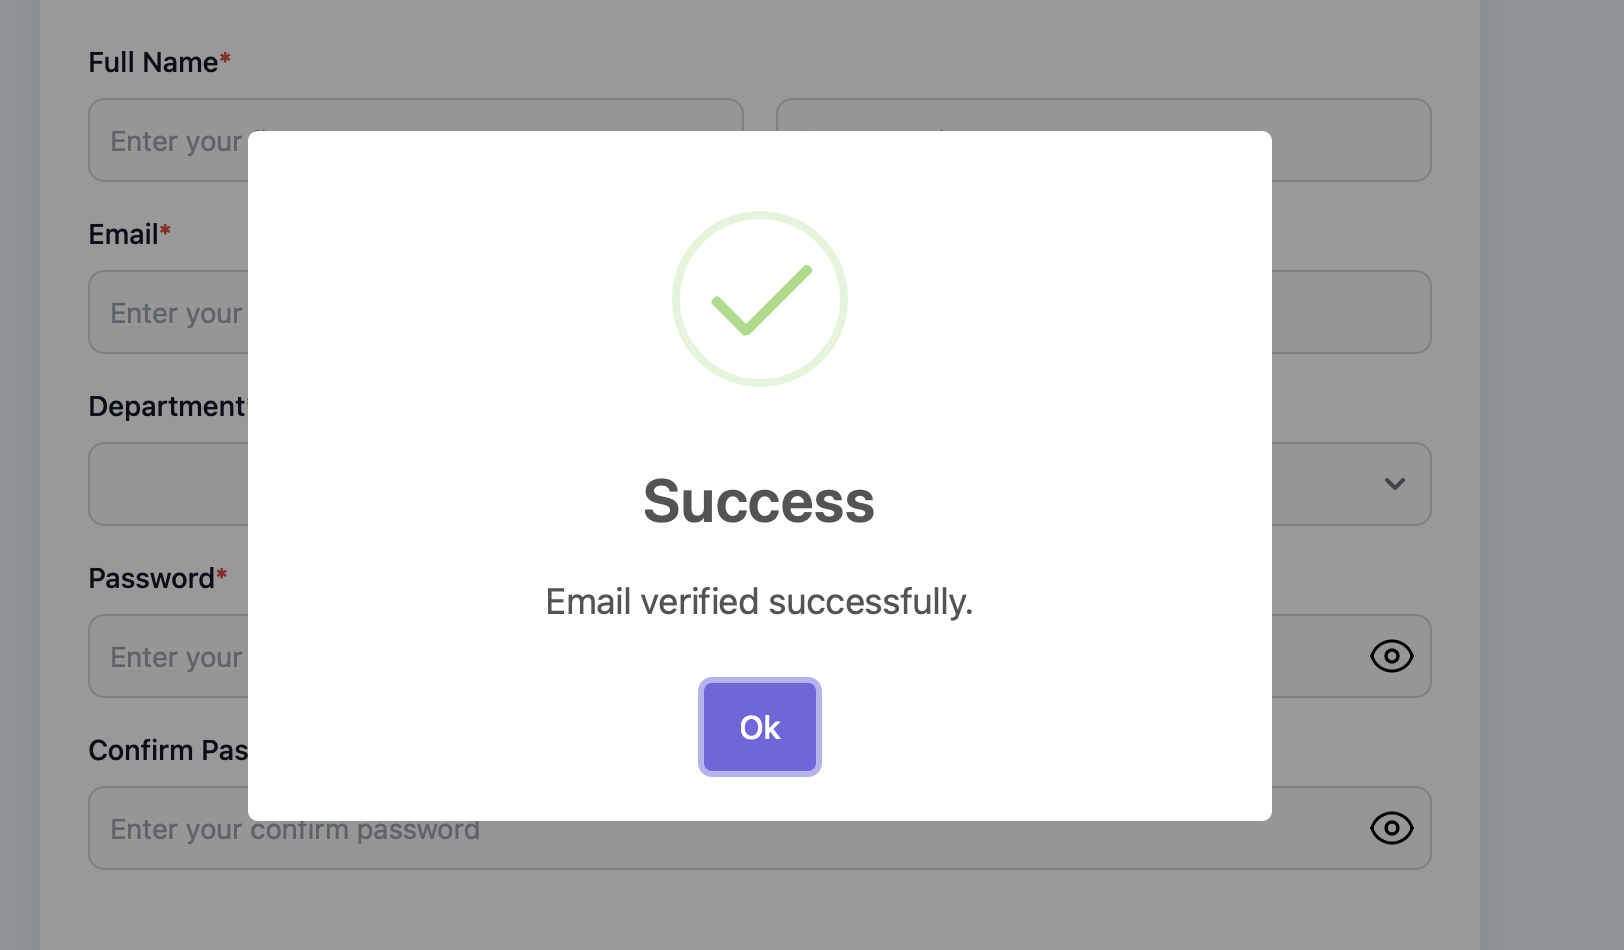
\includegraphics[width=10cm]{Gambar/bab3/user-manual/user-manual-berhasil-verifikasi.png}
    	\caption{Pesan Berhasil Verifikasi \textit{Email}}
    	\label{fig:user-manual-pesan-berhasil-verifikasi}
        \end{figure}
        \FloatBarrier
    \end{enumerate}

    \item Melihat Jadwal Kerja
    \begin{enumerate}
        \item Melakukan \textit{login} pada aplikasi presensi \textit{online} yang terdapat pada \textbf{Manual \ref{item:melakukan-login}}.
        \item Menekan tombol "\textit{Presence}" pada \textit{navigation bar} yang terletak di paling atas. \textbf{\ref{fig:user-manual-tombol-presence-pada-navigation-bar}} menunjukkan tombol \textit{"Presence"} pada \textit{navigation bar}.
        \item Pada halaman \textit{presence}, tekan tombol \textit{"Check Schedule"} yang terletak ditengah halaman. \textbf{\ref{fig:user-manual-tombol-check-schedule}} menunjukkan tombol \textit{"Check Schedule"} yang terletak di tengah halaman \textit{presence}.
        \item Tampilan modal informasi jadwal kerja akan muncul. \textbf{\ref{fig:user-manual-modal-check-schedule}} menunjukkan tampilan modal \textit{check schedule}.
        \begin{figure}[!htbp]
    	\centering
    	
\includegraphics[width=8cm]{Gambar/bab3/user-manual/user-manual-navbar-presence.png}
    	\caption{Tombol \textit{Presence} Pada \textit{Navigation Bar}}
    	\label{fig:user-manual-tombol-presence-pada-navigation-bar}
        \end{figure}
        \FloatBarrier
        \begin{figure}[!htbp]
    	\centering
    	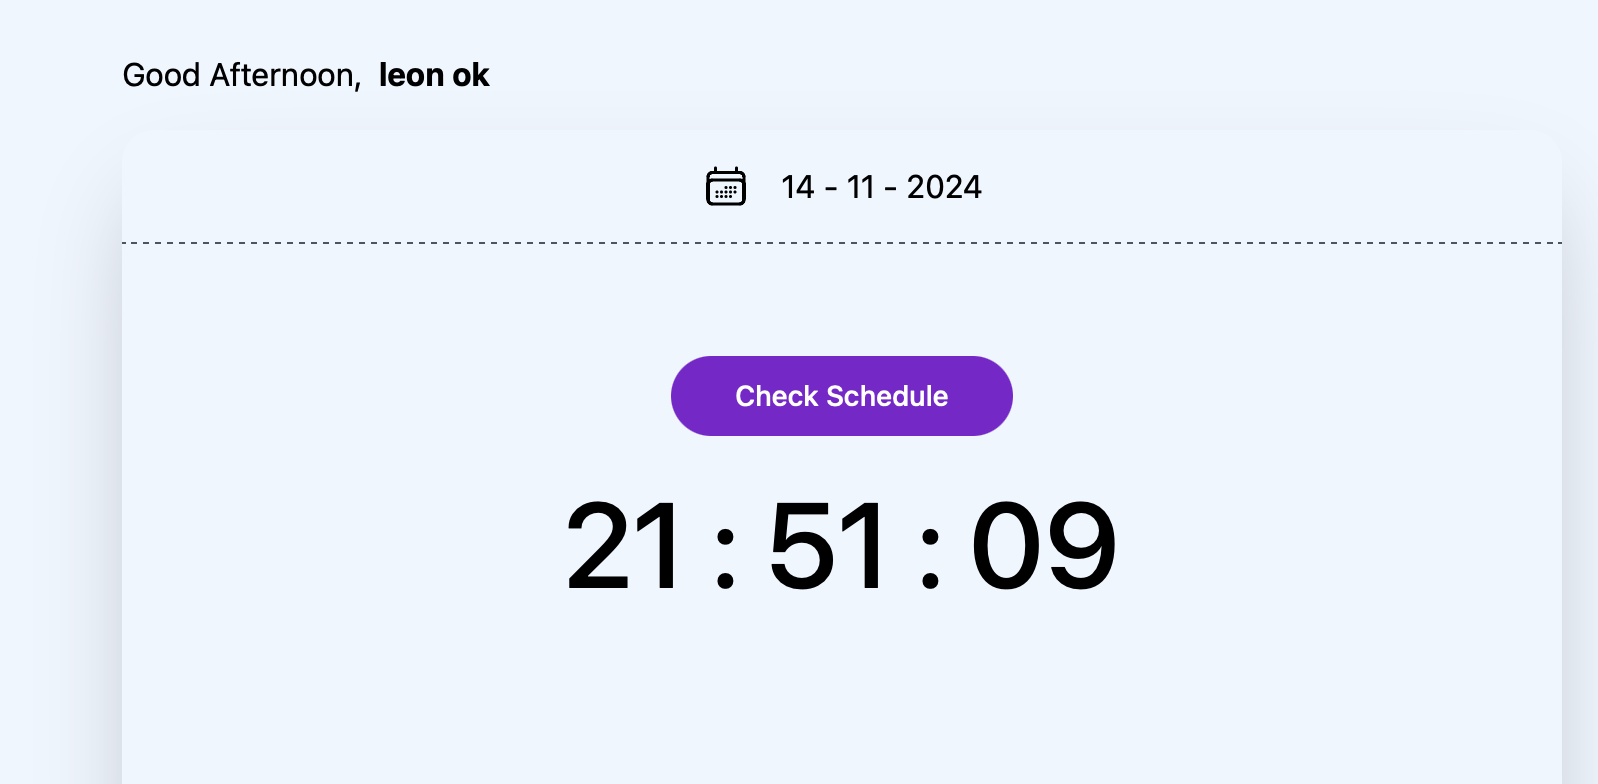
\includegraphics[width=8cm]{Gambar/bab3/user-manual/user-manual-tombol-check-schedule.png}
    	\caption{Tombol \textit{Check Schedule} Pada Halaman \textit{Presence}}
    	\label{fig:user-manual-tombol-check-schedule}
        \end{figure}
        \FloatBarrier
        \begin{figure}[!htbp]
    	\centering
    	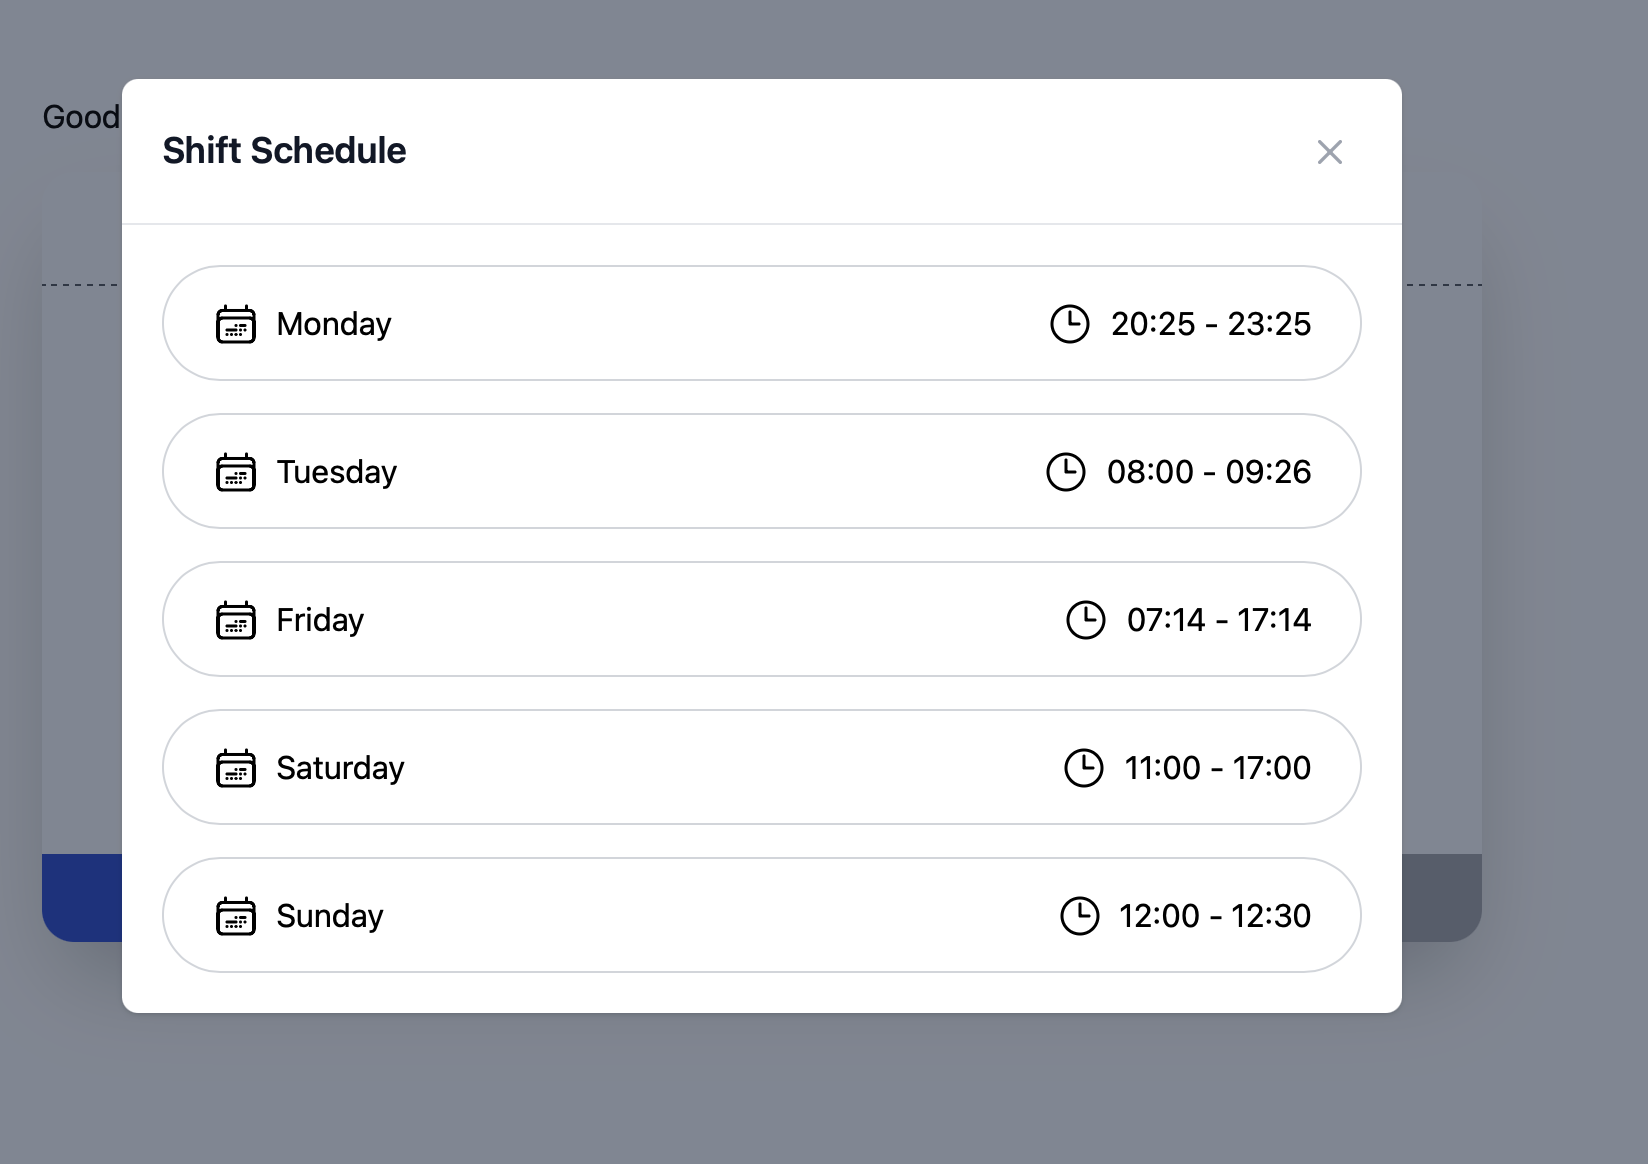
\includegraphics[width=8cm]{Gambar/bab3/user-manual/user-manual-modal-check-schedule.png}
    	\caption{Tampilan Modal \textit{Check Schedule}}
    	\label{fig:user-manual-modal-check-schedule}
        \end{figure}
        \FloatBarrier
    \end{enumerate}

    \item Melakukan \textit{Clock In}
    \begin{enumerate}
        \item Melakukan \textit{login} pada aplikasi presensi \textit{online} yang terdapat pada \textbf{Manual \ref{item:melakukan-login}}.
        \item Menekan tombol "\textit{Presence}" pada \textit{navigation bar} yang terletak di paling atas. \textbf{\ref{fig:user-manual-tombol-presence-pada-navigation-bar}} menunjukkan tombol \textit{"Presence"} pada \textit{navigation bar}.
        \item Pada halaman \textit{presence}, tekan tombol \textit{"Clock In"} yang berada ditengah halaman dan izinkan perangkat untuk mengakses lokasi. \textbf{\ref{fig:user-manual-tombol-clock-in}} menunjukkan tombol "\textit{Clock In}" pada halaman \textit{presence}.
        \begin{figure}[!htbp]
    	\centering
    	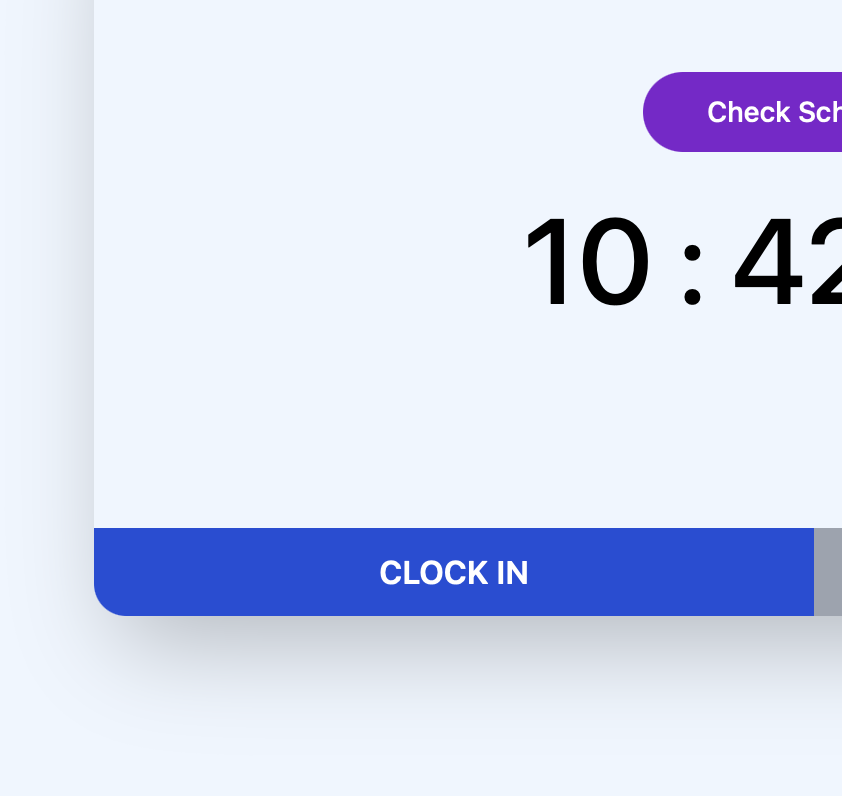
\includegraphics[width=8cm]{Gambar/bab3/user-manual/user-manual-tombol-clock-in.png}
    	\caption{Tombol \textit{Clock In} Pada Halaman \textit{Presence}}
    	\label{fig:user-manual-tombol-clock-in}
        \end{figure}
        \FloatBarrier
        \item Mengisi seluruh \textit{input form} pada modal \textit{clock in}. \textbf{\ref{fig:user-manual-modal-clock-in}} menunjukkan tampilan modal \textit{clock in}.
        \begin{figure}[!htbp]
    	\centering
    	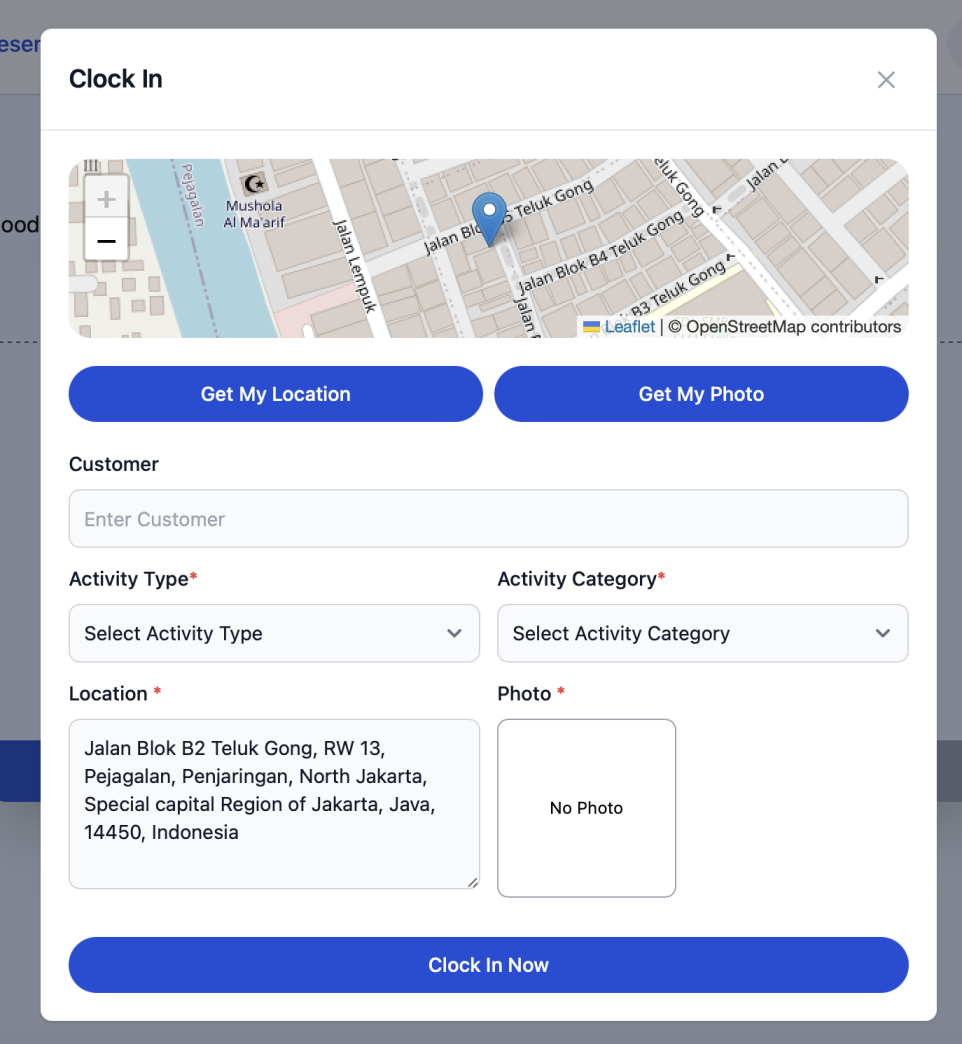
\includegraphics[width=5cm]{Gambar/bab3/user-manual/user-manual-modal-clock-in.png}
    	\caption{Modal \textit{Clock In}}
    	\label{fig:user-manual-modal-clock-in}
        \end{figure}
        \FloatBarrier
        \item Menekan tombol "\textit{Get My Photo}" pada modal \textit{clock in} untuk mengambil foto presensi dan izinkan perangkat untuk mengakses kamera. \textbf{\ref{fig:user-manual-tombol-get-my-photo-pada-modal-clock-in}} menunjukkan tombol "\textit{Get My Photo}" pada modal \textit{clock in}.
        \begin{figure}[!htbp]
    	\centering
    	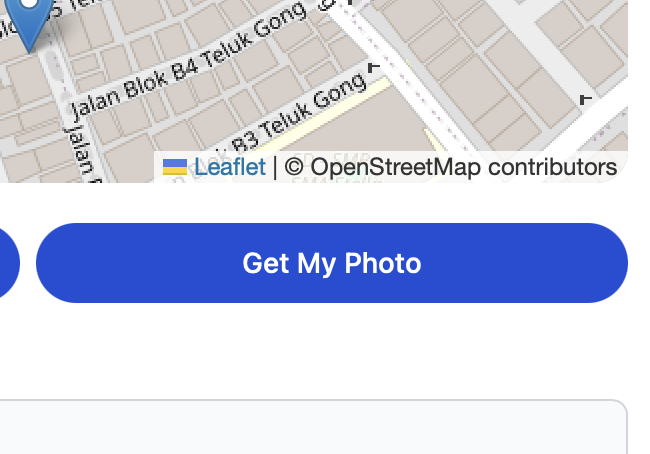
\includegraphics[width=8cm]{Gambar/bab3/user-manual/user-manual-tombol-get-my-photo-clock-in.png}
    	\caption{Tombol \textit{Get My Photo} Pada Modal \textit{Clock In}}
    	\label{fig:user-manual-tombol-get-my-photo-pada-modal-clock-in}
        \end{figure}
        \FloatBarrier

        \item Mengambil foto wajah pada modal kamera, pastikan posisi kepala berada ditengah lingkaran yang telah ditentukan pada kamera dan tekan tombol bulat untuk mengambil foto. \textbf{\ref{fig:user-manual-modal-kamera-clock-in}} menunjukkan tampilan modal kamera saat \textit{clock in}.
        \begin{figure}[!htbp]
    	\centering
    	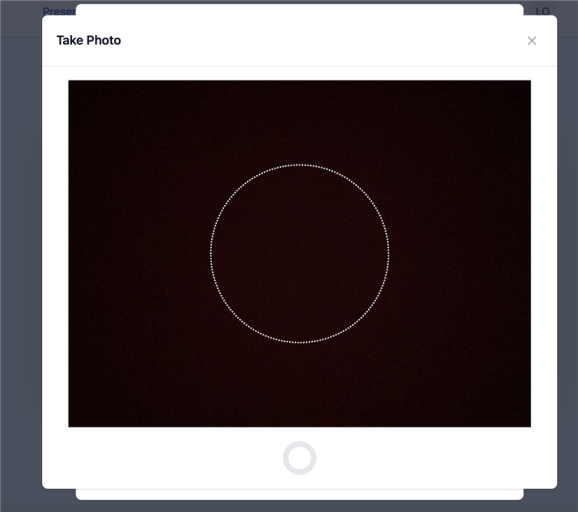
\includegraphics[width=8cm]{Gambar/bab3/user-manual/user-manual-modal-kamera-clock-in.png}
    	\caption{Modal Kamera \textit{Clock In}}
    	\label{fig:user-manual-modal-kamera-clock-in}
        \end{figure}
        \FloatBarrier
        \item Saat berhasil ambil foto, maka modal kamera akan tertutup dan membuka modal \textit{clock in} kembali. Tekan tombol \textit{"Clock In Now"} untuk menyimpan presensi masuk. \textbf{\ref{fig:user-manual-tombol-clock-in-now-pada-modal-clock-in}} menunjukkan tombol "\textit{Clock In Now}" pada modal \textit{clock in}.
        \begin{figure}[!htbp]
    	\centering
    	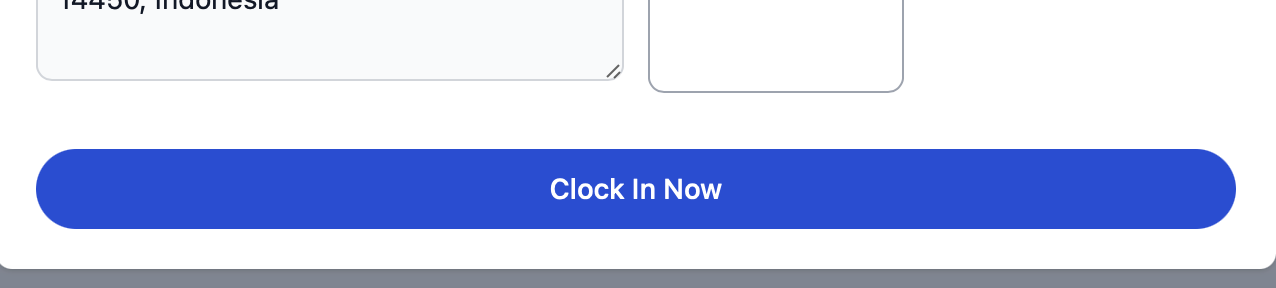
\includegraphics[width=8cm]{Gambar/bab3/user-manual/user-manual-tombol-clock-in-now.png}
    	\caption{Tombol \textit{Clock In Now} Pada Modal \textit{Clock In}}
    	\label{fig:user-manual-tombol-clock-in-now-pada-modal-clock-in}
        \end{figure}
        \FloatBarrier
    \end{enumerate}

    \item Melakukan \textit{Clock Out}
    \begin{enumerate}
        \item Melakukan \textit{login} pada aplikasi presensi \textit{online} yang terdapat pada \textbf{Manual \ref{item:melakukan-login}}.
        \item Menekan tombol "\textit{Presence}" pada \textit{navigation bar} yang terletak di paling atas. \textbf{\ref{fig:user-manual-tombol-presence-pada-navigation-bar}} menunjukkan tombol \textit{"Presence"} pada \textit{navigation bar}.
        \item Pastikan sudah melakukan \textit{clock in} sebelumya, pada halaman \textit{presence}, tekan tombol \textit{"Clock Out"} yang berada ditengah halaman dan izinkan perangkat untuk mengakses lokasi. \textbf{\ref{fig:user-manual-tombol-clock-out}} menunjukkan tombol "\textit{Clock Out}" pada halaman \textit{presence}.
        \begin{figure}[!htbp]
    	\centering
    	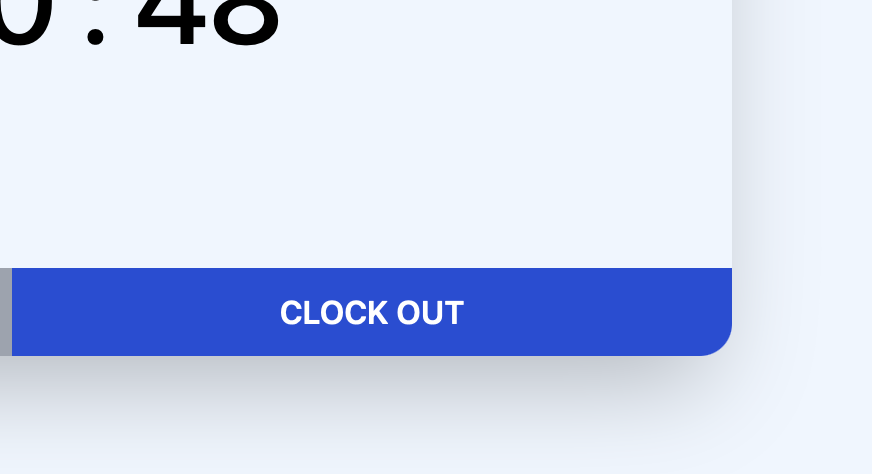
\includegraphics[width=8cm]{Gambar/bab3/user-manual/user-manual-tombol-clock-out.png}
    	\caption{Tombol \textit{Clock Out} Pada Halaman \textit{Presence}}
    	\label{fig:user-manual-tombol-clock-out}
        \end{figure}
        \FloatBarrier
        \item Seluruh \textit{input form} pada modal \textit{clock out} dapat dilakukan perubahan. \textbf{\ref{fig:user-manual-modal-clock-out}} menunjukkan tampilan modal \textit{clock out}.
        \begin{figure}[!htbp]
    	\centering
    	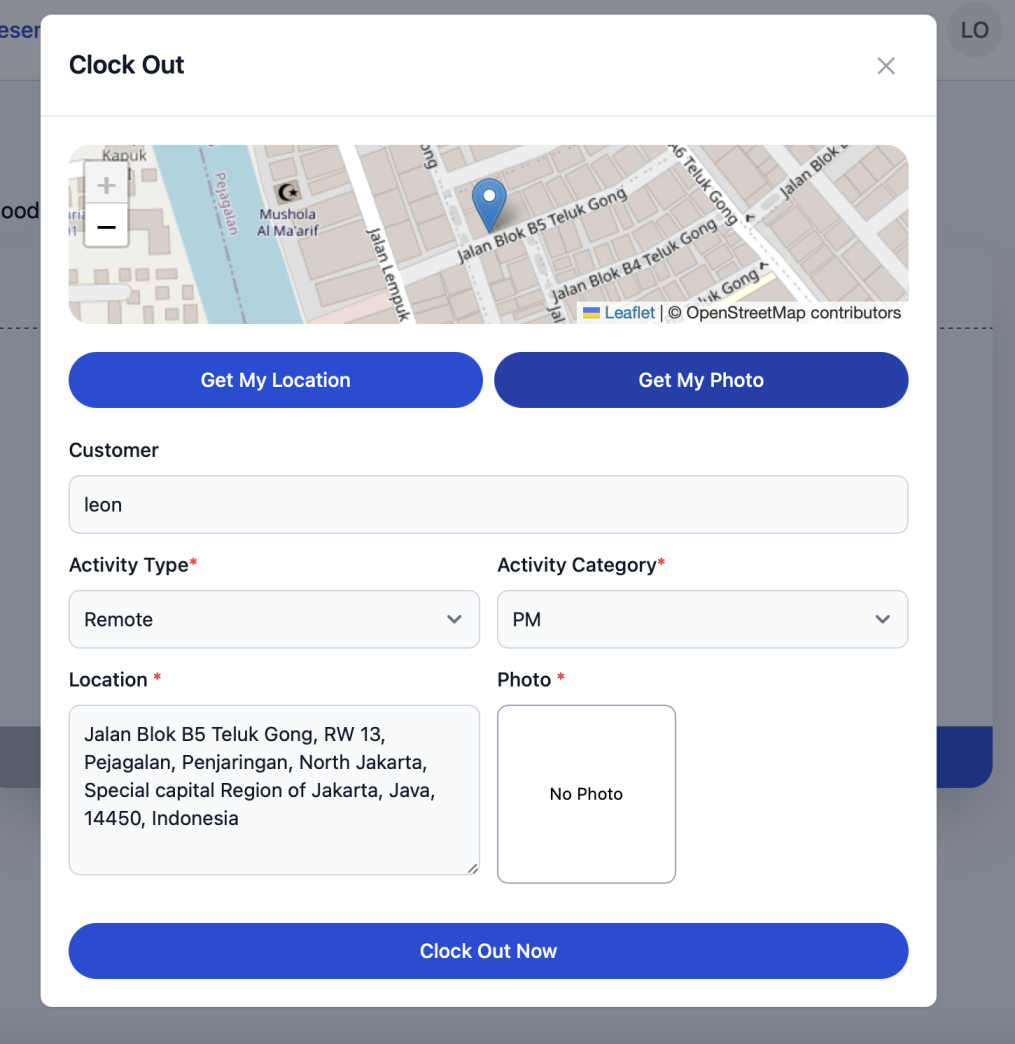
\includegraphics[width=5cm]{Gambar/bab3/user-manual/user-manual-modal-clock-out.png}
    	\caption{Modal \textit{Clock Out}}
    	\label{fig:user-manual-modal-clock-out}
        \end{figure}
        \FloatBarrier
        \item Menekan tombol "\textit{Get My Photo}" pada modal \textit{clock out} untuk mengambil foto presensi dan izinkan perangkat untuk mengakses kamera. \textbf{\ref{fig:user-manual-tombol-get-my-photo-pada-modal-clock-out}} menunjukkan tombol "\textit{Get My Photo}" pada modal \textit{clock out}.
        \begin{figure}[!htbp]
    	\centering
    	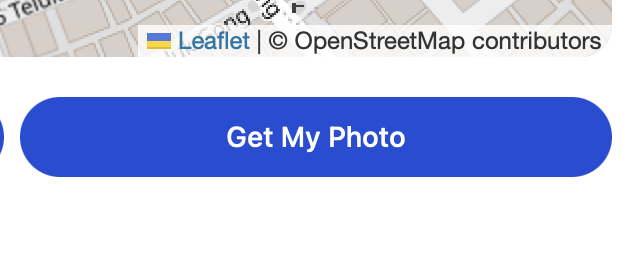
\includegraphics[width=8cm]{Gambar/bab3/user-manual/user-manual-get-my-photo-clock-out.png}
    	\caption{Tombol \textit{Get My Photo} Pada Modal \textit{Clock Out}}
    	\label{fig:user-manual-tombol-get-my-photo-pada-modal-clock-out}
        \end{figure}
        \FloatBarrier

        \item Mengambil foto wajah pada modal kamera, pastikan posisi kepala berada ditengah lingkaran yang telah ditentukan pada kamera dan tekan tombol bulat untuk mengambil foto. \textbf{\ref{fig:user-manual-modal-kamera-clock-out}} menunjukkan tampilan modal kamera saat \textit{clock out}.
        \begin{figure}[!htbp]
    	\centering
    	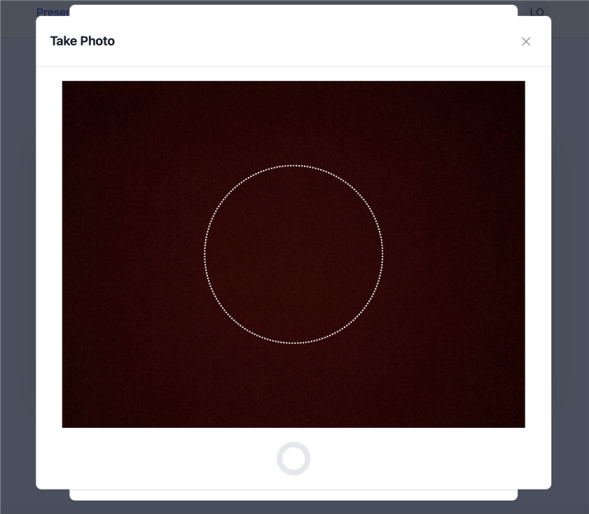
\includegraphics[width=8cm]{Gambar/bab3/user-manual/user-manual-modal-kamera-clock-out.png}
    	\caption{Modal Kamera \textit{Clock Out}}
    	\label{fig:user-manual-modal-kamera-clock-out}
        \end{figure}
        \FloatBarrier
        \item Saat berhasil ambil foto, maka modal kamera akan tertutup dan membuka modal \textit{clock out} kembali. Tekan tombol \textit{"Clock Out Now"} untuk menyimpan presensi keluar. \textbf{\ref{fig:user-manual-tombol-clock-out-now-pada-modal-clock-out}} menunjukkan tombol "\textit{Clock Out Now}" pada modal \textit{clock in}.
        \begin{figure}[!htbp]
    	\centering
    	
\includegraphics[width=8cm]{Gambar/bab3/user-manual/user-manual-tombol-clock-out-now.png}
    	\caption{Tombol \textit{Clock Out Now} Pada Modal \textit{Clock Out}}
    	\label{fig:user-manual-tombol-clock-out-now-pada-modal-clock-out}
        \end{figure}
        \FloatBarrier
    \end{enumerate}

    \item Melakukan Pengajuan Lembur Manual
    \begin{enumerate}
        \item Melakukan \textit{login} pada aplikasi presensi \textit{online} yang terdapat pada \textbf{Manual \ref{item:melakukan-login}}.
        \item Menekan tombol "\textit{Request}" pada \textit{navigation bar} yang terletak di paling atas. \textbf{\ref{fig:user-manual-tombol-request-pada-navigation-bar}} menunjukkan tombol \textit{"Request"} pada \textit{navigation bar}.
        \begin{figure}[!htbp]
    	\centering
    	
\includegraphics[width=8cm]{Gambar/bab3/user-manual/user-manual-navbar-request.png}
    	\caption{Tombol \textit{Request} Pada \textit{Navigation Bar}}
    	\label{fig:user-manual-tombol-request-pada-navigation-bar}
        \end{figure}
        \FloatBarrier
        \item Mengisi seluruh \textit{input form} pada halaman \textit{request} dan tekan tombol \textit{"Submit"} untuk menyimpan data pengajuan lembur. \textbf{\ref{fig:user-manual-halaman-pengajuan-lembur-manual}} menunjukkan halaman pengajuan lembur manual.
        \begin{figure}[!htbp]
    	\centering
    	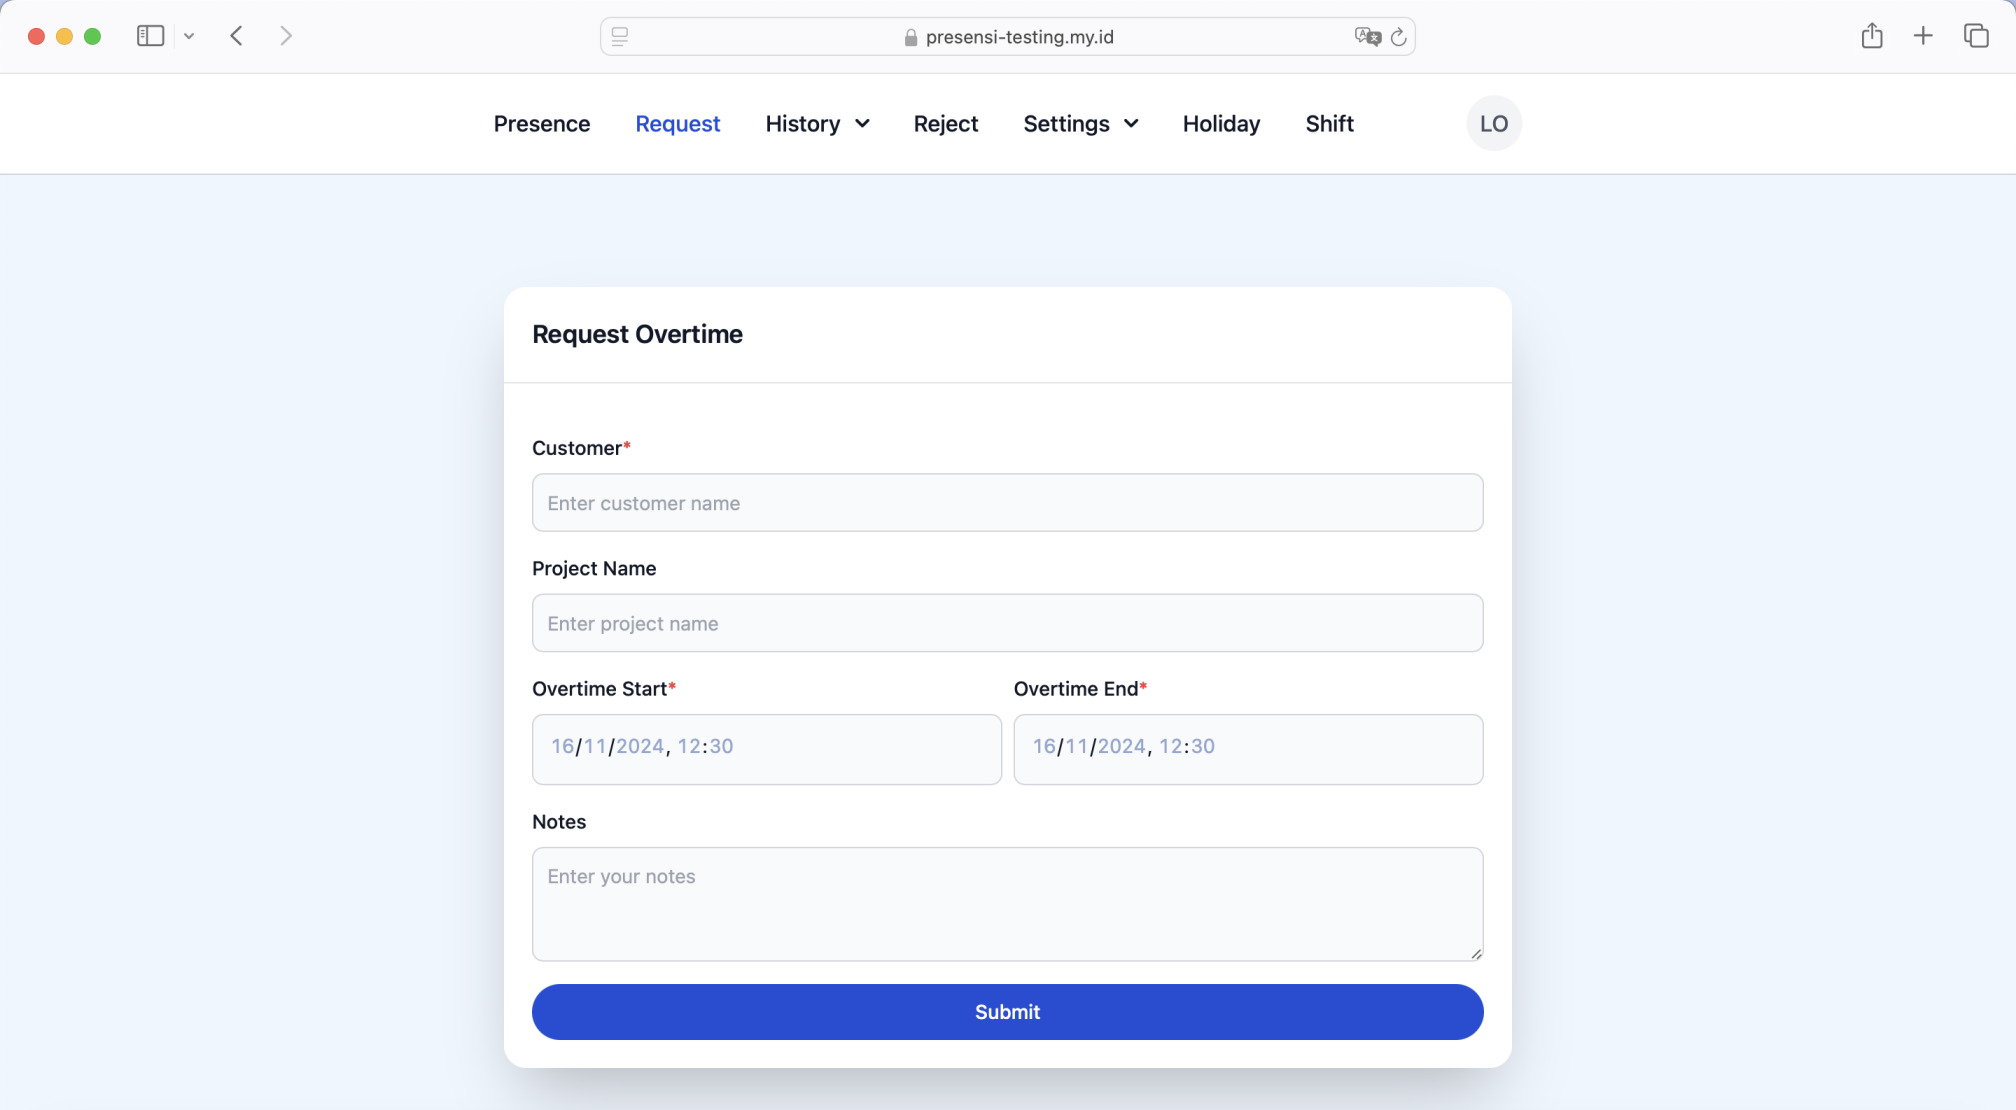
\includegraphics[width=8cm]{Gambar/bab3/user-manual/user-manual-pengajuan-lembur-manual.png}
    	\caption{Tampilan Halaman Pengajuan Lembur Manual}
    	\label{fig:user-manual-halaman-pengajuan-lembur-manual}
        \end{figure}
        \FloatBarrier
    \end{enumerate}

    \item Melihat Riwayat Presensi\label{item:melihat-riwayat-presensi}
    \begin{enumerate}
        \item Melakukan \textit{login} pada aplikasi presensi \textit{online} yang terdapat pada \textbf{Manual \ref{item:melakukan-login}}.
        \item Menekan tombol "\textit{History}" pada \textit{navigation bar} yang terletak di paling atas dan memilih tombol \textit{"Attendance History"}. \textbf{\ref{fig:user-manual-tombol-attendance-history-pada-navigation-bar}} menunjukkan tombol \textit{"Attendance History"} pada \textit{navigation bar}.
        \begin{figure}[!htbp]
    	\centering
    	
\includegraphics[width=8cm]{Gambar/bab3/user-manual/user-manual-navbar-attendance-history.png}
    	\caption{Tombol \textit{Attendance History} Pada \textit{Navigation Bar}}
    	\label{fig:user-manual-tombol-attendance-history-pada-navigation-bar}
        \end{figure}
        \FloatBarrier
        \item Seluruh daftar data riwayat presensi akan ditampilkan pada halaman \textit{attendance history}. \textbf{\ref{fig:user-manual-halaman-riwayat-presensi}} menunjukkan halaman \textit{attendance history}. 
        \begin{figure}[!htbp]
    	\centering
    	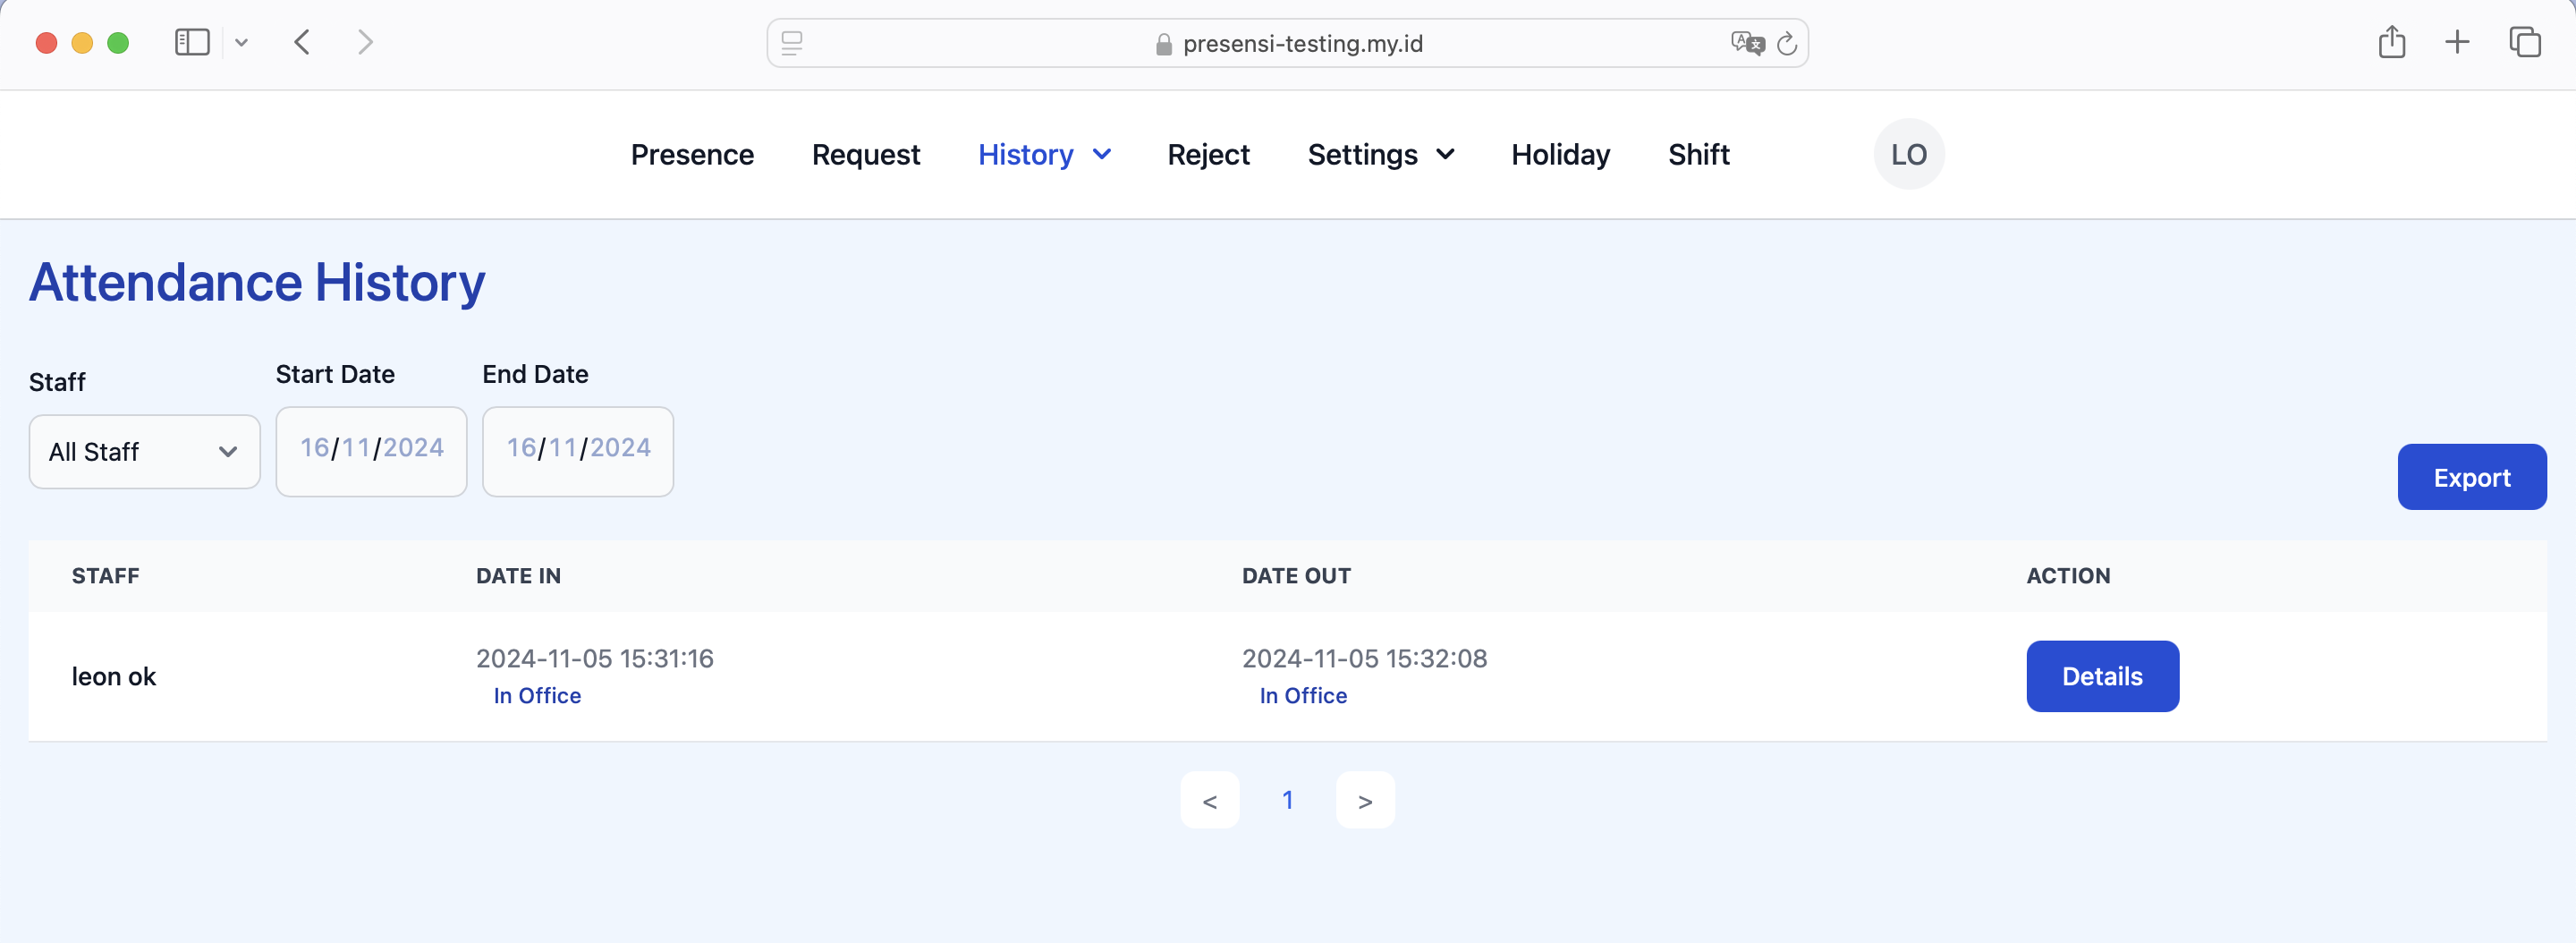
\includegraphics[width=8cm]{Gambar/bab3/user-manual/user-manual-halaman-riwayat-presensi.png}
    	\caption{Halaman \textit{Attendance History}}
    	\label{fig:user-manual-halaman-riwayat-presensi}
        \end{figure}
        \FloatBarrier
    \end{enumerate}

    \item Melihat Detail Riwayat Presensi
    \begin{enumerate}
        \item Membuka halaman riwayat presensi yang terdapat pada \textbf{Manual \ref{item:melihat-riwayat-presensi}}.
        \item Menekan tombol "\textit{Detail}" pada salah satu data presensi. Sistem akan menampilkan modal detail riwayat presensi beserta informasi lengkap riwayat presensi. \textbf{\ref{fig:user-manual-modal-attendance-history-details}} menunjukkan modal \textit{attendance history details}.
        \begin{figure}[!htbp]
    	\centering
    	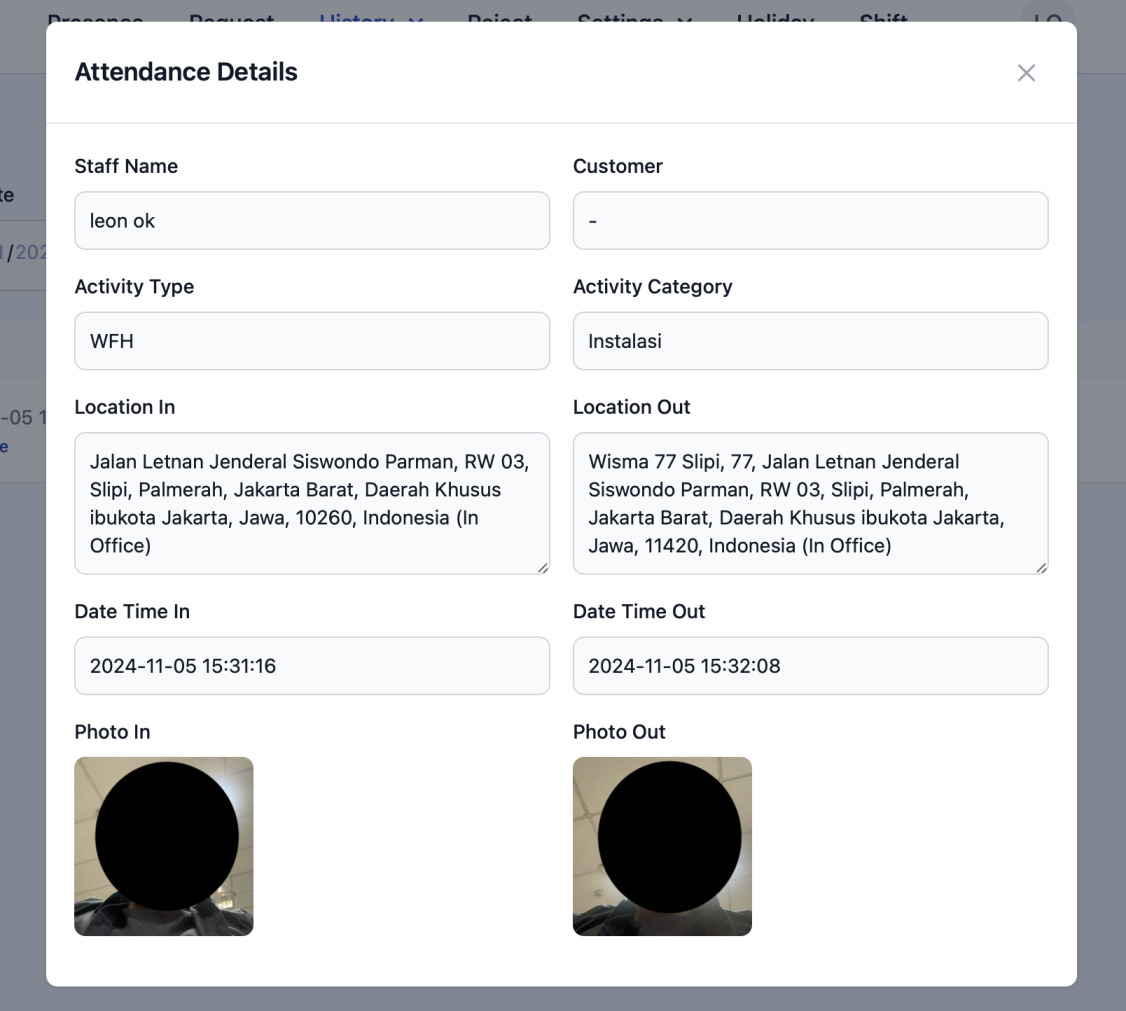
\includegraphics[width=8cm]{Gambar/bab3/user-manual/user-manual-detail-riwayat-presensi.png}
    	\caption{Modal \textit{Attendance History Details}}
    	\label{fig:user-manual-modal-attendance-history-details}
        \end{figure}
        \FloatBarrier
    \end{enumerate}

    \item Melakukan \textit{Export} Data Riwayat Presensi
    \begin{enumerate}
        \item Membuka halaman riwayat presensi yang terdapat pada \textbf{Manual \ref{item:melihat-riwayat-presensi}}.
        \item Menekan tombol \textit{"Export"} yang terdapat pada halaman riwayat presensi. \textbf{\ref{fig:user-manual-tombol-export-riwayat-presensi}} menunjukkan tombol untuk \textit{export} riwayat presensi menjadi format \textit{Excel}.
        \begin{figure}[!htbp]
    	\centering
    	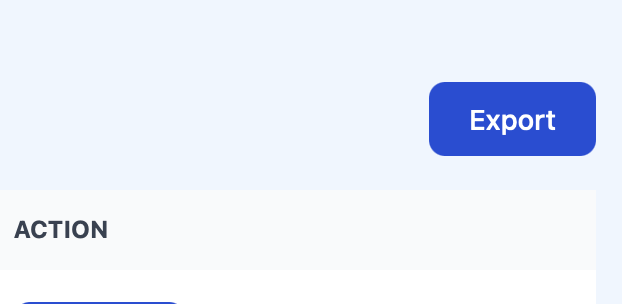
\includegraphics[width=8cm]{Gambar/bab3/user-manual/user-manual-tombol-export-riwayat-presensi.png}
    	\caption{Tombol \textit{Export} Riwayat Presensi}
    	\label{fig:user-manual-tombol-export-riwayat-presensi}
        \end{figure}
        \FloatBarrier
        \item Perangkat akan otomatis men-\textit{download file Excel} yang berisi data presensi. \textbf{\ref{fig:user-manual-file-excel-riwayat-presensi}} menunjukkan \textit{file Excel} riwayat presensi yang telah di-\textit{donwload}.
        \begin{figure}[!htbp]
    	\centering
    	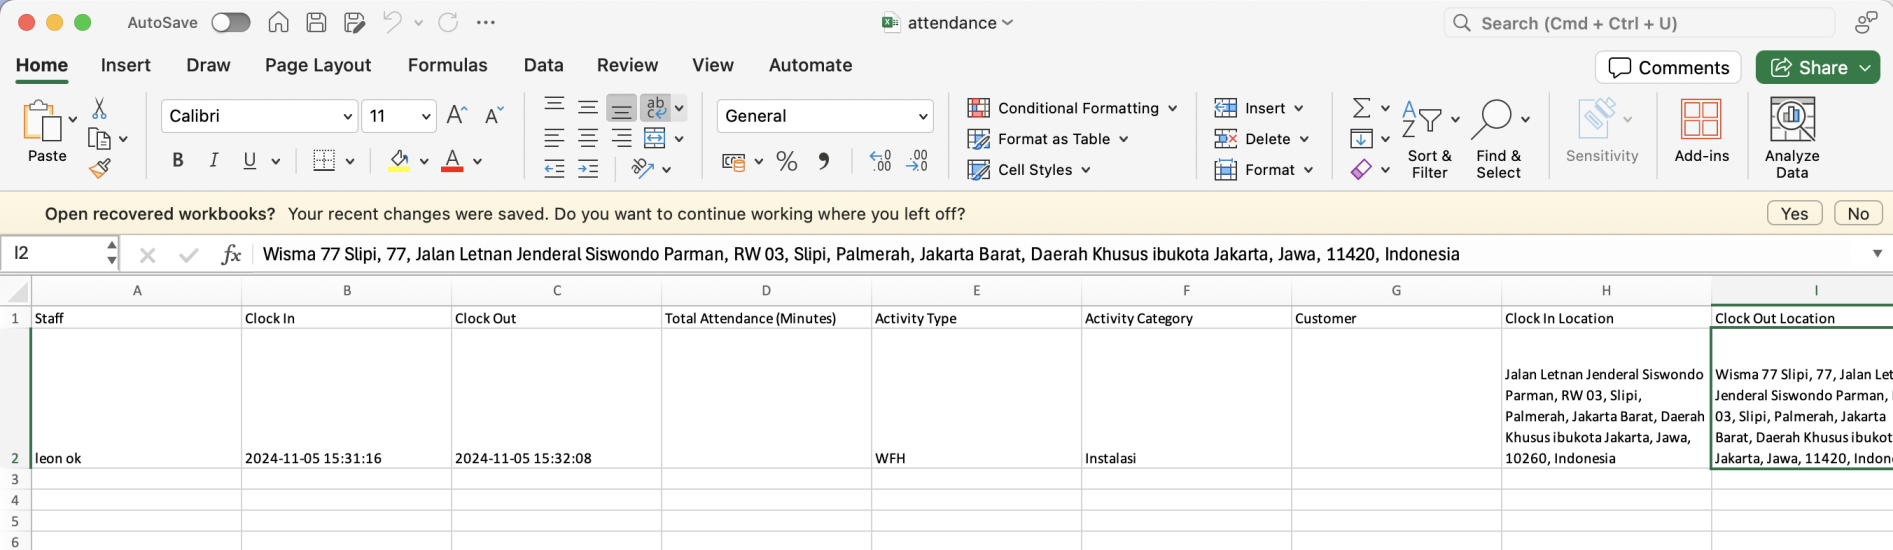
\includegraphics[width=8cm]{Gambar/bab3/user-manual/user-manual-file-excel-riwayat-presensi.png}
    	\caption{\textit{File Excel} Riwayat Presensi}
    	\label{fig:user-manual-file-excel-riwayat-presensi}
        \end{figure}
        \FloatBarrier
    \end{enumerate}

    \item Melihat Riwayat Lembur\label{item:melihat-riwayat-lembur}
    \begin{enumerate}
        \item Melakukan \textit{login} pada aplikasi presensi \textit{online} yang terdapat pada \textbf{Manual \ref{item:melakukan-login}}.
        \item Menekan tombol "\textit{History}" pada \textit{navigation bar} yang terletak di paling atas dan memilih tombol \textit{"Overtime History"}. \textbf{\ref{fig:user-manual-tombol-overtime-history-pada-navigation-bar}} menunjukkan tombol \textit{"Overtime History"} pada \textit{navigation bar}.
        \begin{figure}[!htbp]
    	\centering
    	
\includegraphics[width=8cm]{Gambar/bab3/user-manual/user-manual-navbar-overtime-history.png}
    	\caption{Tombol \textit{Overtime History} Pada \textit{Navigation Bar}}
    	\label{fig:user-manual-tombol-overtime-history-pada-navigation-bar}
        \end{figure}
        \FloatBarrier
        \item Seluruh daftar data riwayat lembur akan ditampilkan pada halaman \textit{overtime history}. \textbf{\ref{fig:user-manual-halaman-riwayat-lembur}} menunjukkan halaman \textit{overtime history}. 
        \begin{figure}[!htbp]
    	\centering
    	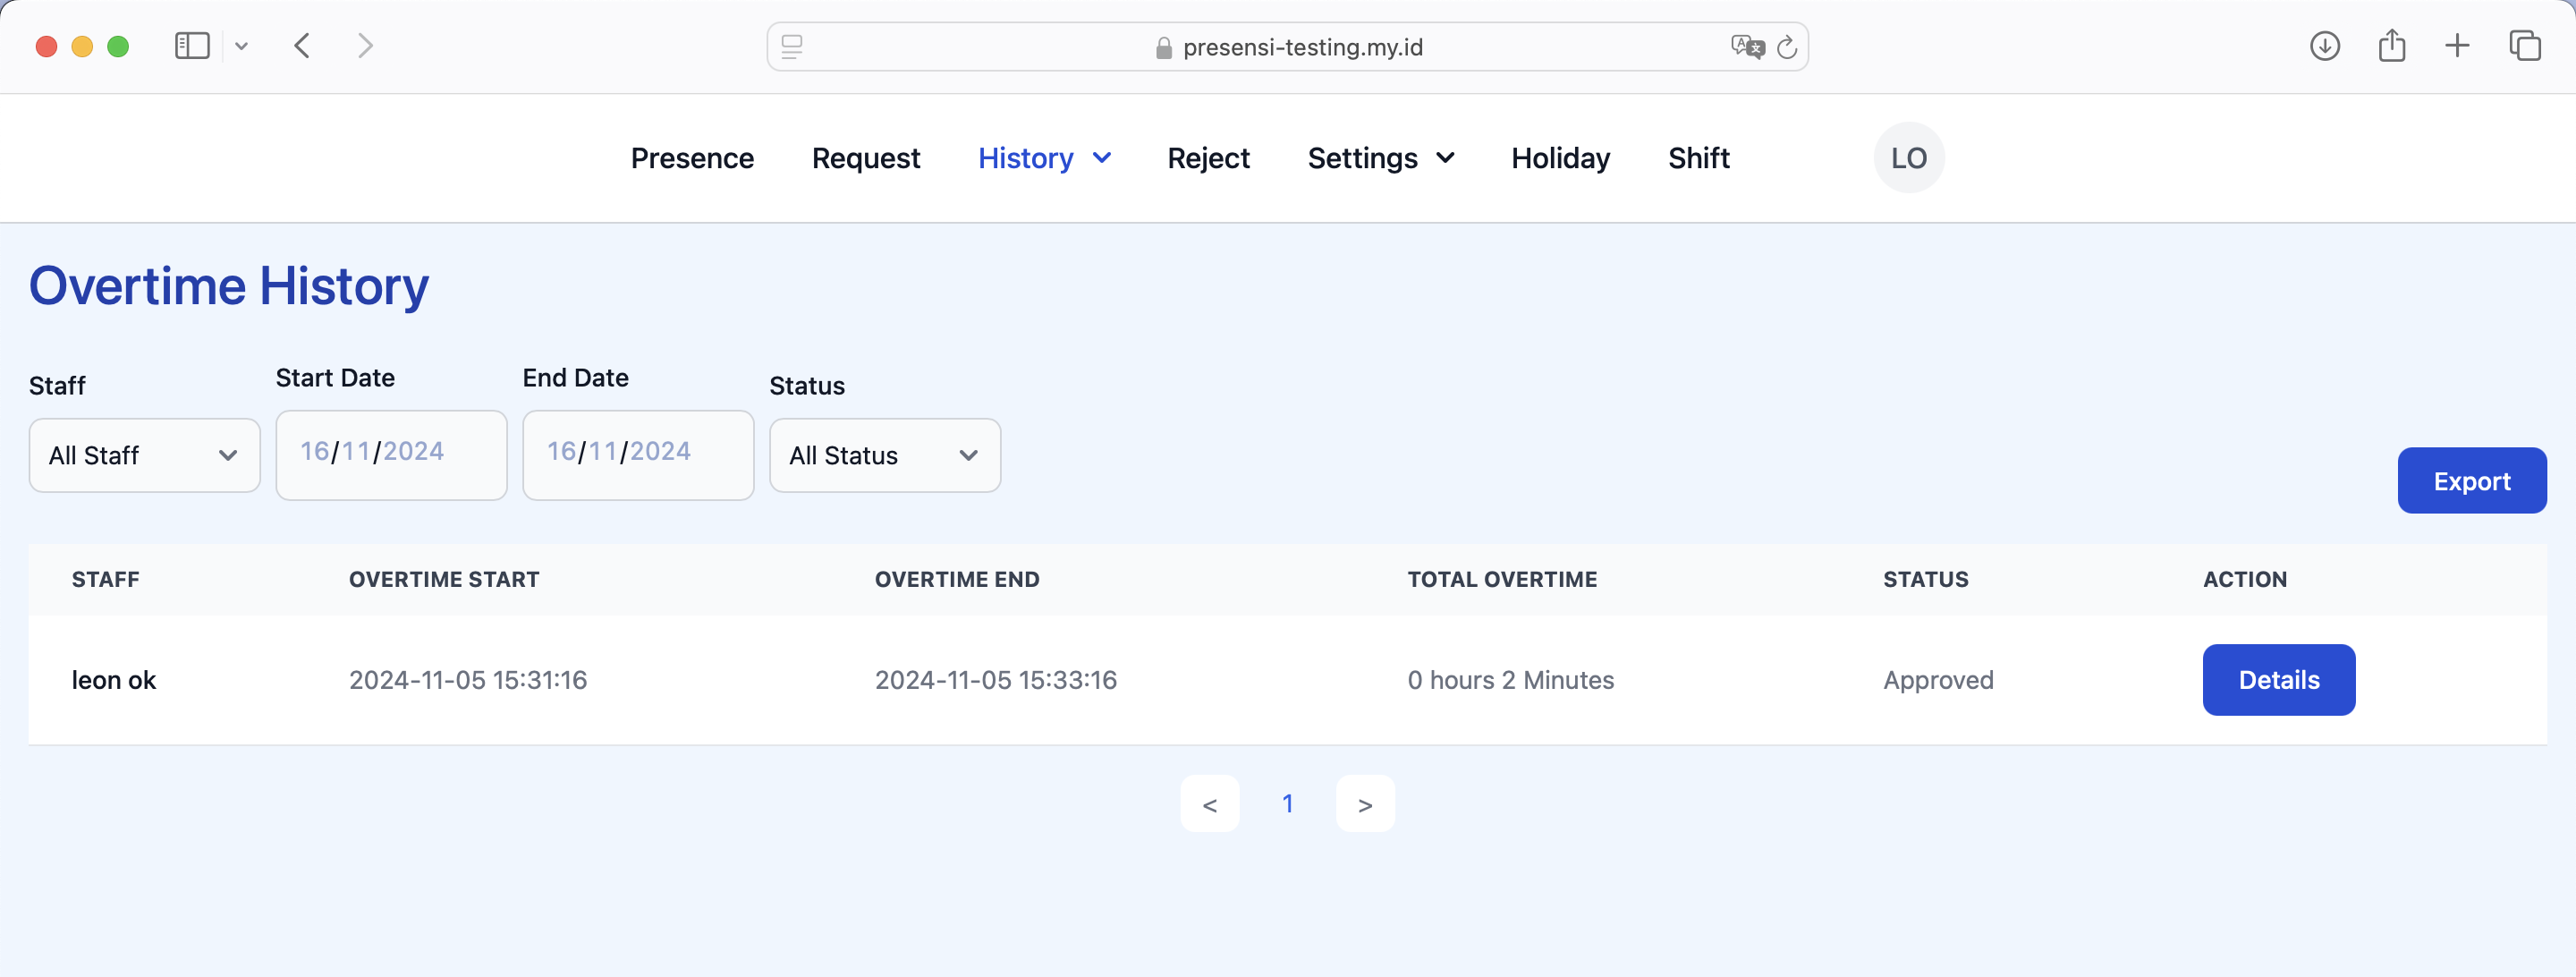
\includegraphics[width=8cm]{Gambar/bab3/user-manual/user-manual-halaman-riwayat-lembur.png}
    	\caption{Halaman \textit{Overtime History}}
    	\label{fig:user-manual-halaman-riwayat-lembur}
        \end{figure}
        \FloatBarrier
    \end{enumerate}

    \item Melihat Detail Riwayat Lembur
    \begin{enumerate}
        \item Membuka halaman riwayat lembur yang terdapat pada \textbf{Manual \ref{item:melihat-riwayat-lembur}}.
        \item Menekan tombol "\textit{Detail}" pada salah satu data lembur. Sistem akan menampilkan modal detail riwayat lembur beserta informasi lengkap riwayat lembur. \textbf{\ref{fig:user-manual-modal-overtime-history-details}} menunjukkan modal \textit{overtime history details}.
        \begin{figure}[!htbp]
    	\centering
    	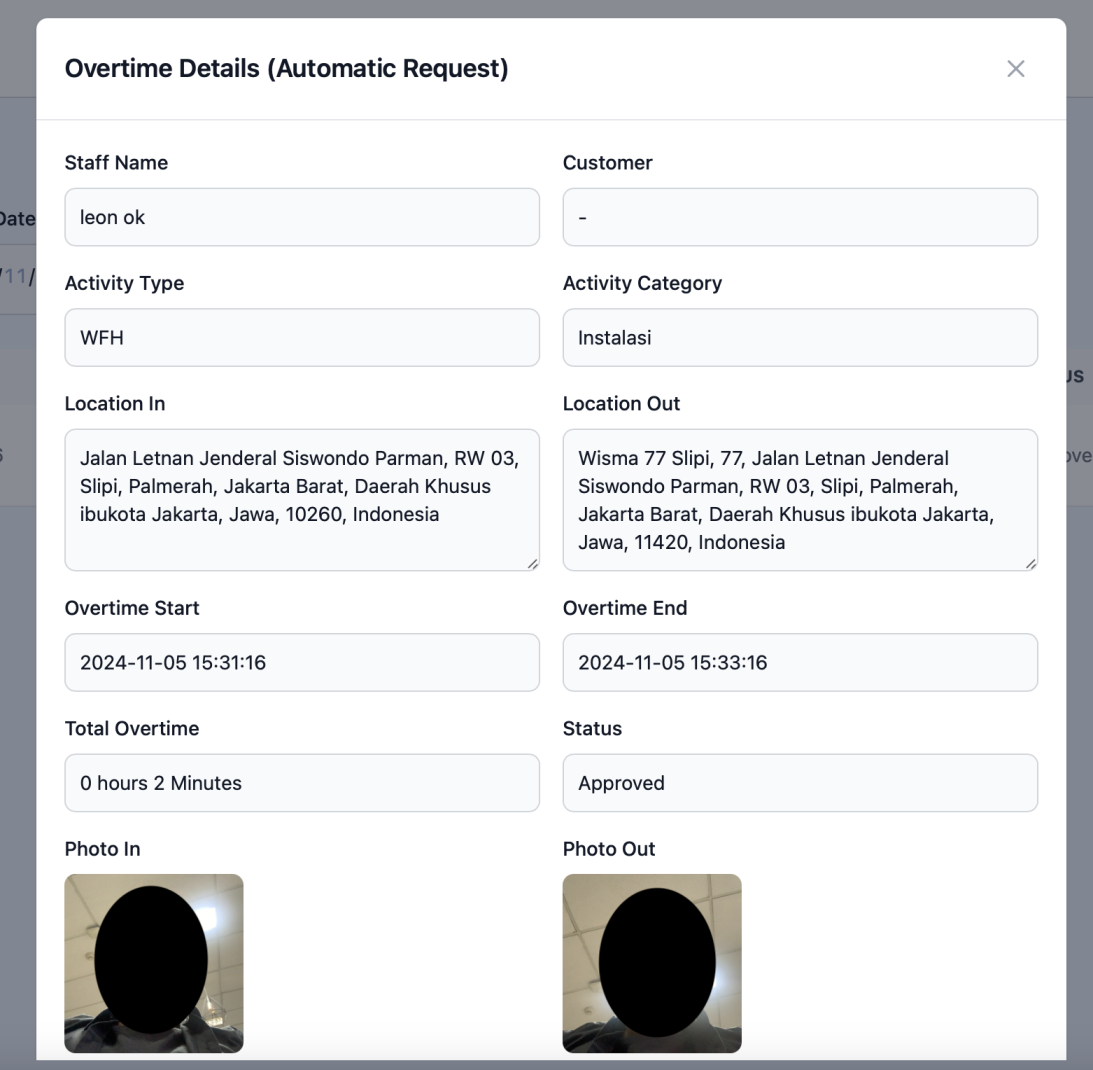
\includegraphics[width=8cm]{Gambar/bab3/user-manual/user-manual-detail-riwayat-lembur.png}
    	\caption{Modal \textit{Overtime History Details}}
    	\label{fig:user-manual-modal-overtime-history-details}
        \end{figure}
        \FloatBarrier
    \end{enumerate}

    \item Melakukan \textit{Export} Data Riwayat Lembur
    \begin{enumerate}
        \item Membuka halaman riwayat lembur yang terdapat pada \textbf{Manual \ref{item:melihat-riwayat-lembur}}.
        \item Menekan tombol \textit{"Export"} yang terdapat pada halaman riwayat lembur. \textbf{\ref{fig:user-manual-tombol-export-riwayat-lembur}} menunjukkan tombol untuk \textit{export} riwayat lembur menjadi format \textit{Excel}.
        \begin{figure}[!htbp]
    	\centering
    	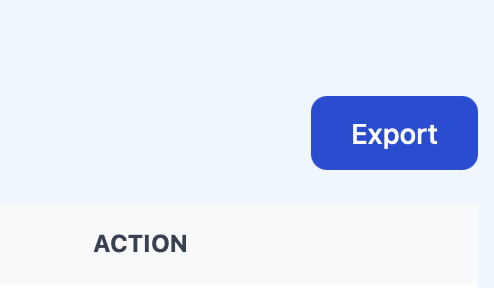
\includegraphics[width=8cm]{Gambar/bab3/user-manual/user-manual-tombol-export-riwayat-lembur.png}
    	\caption{Tombol \textit{Export} Riwayat Lembur}
    	\label{fig:user-manual-tombol-export-riwayat-lembur}
        \end{figure}
        \FloatBarrier
        \item Perangkat akan otomatis men-\textit{download file Excel} yang berisi data lembur. \textbf{\ref{fig:user-manual-file-excel-riwayat-lembur}} menunjukkan \textit{file Excel} riwayat lembur yang telah di-\textit{donwload}.
        \begin{figure}[!htbp]
    	\centering
    	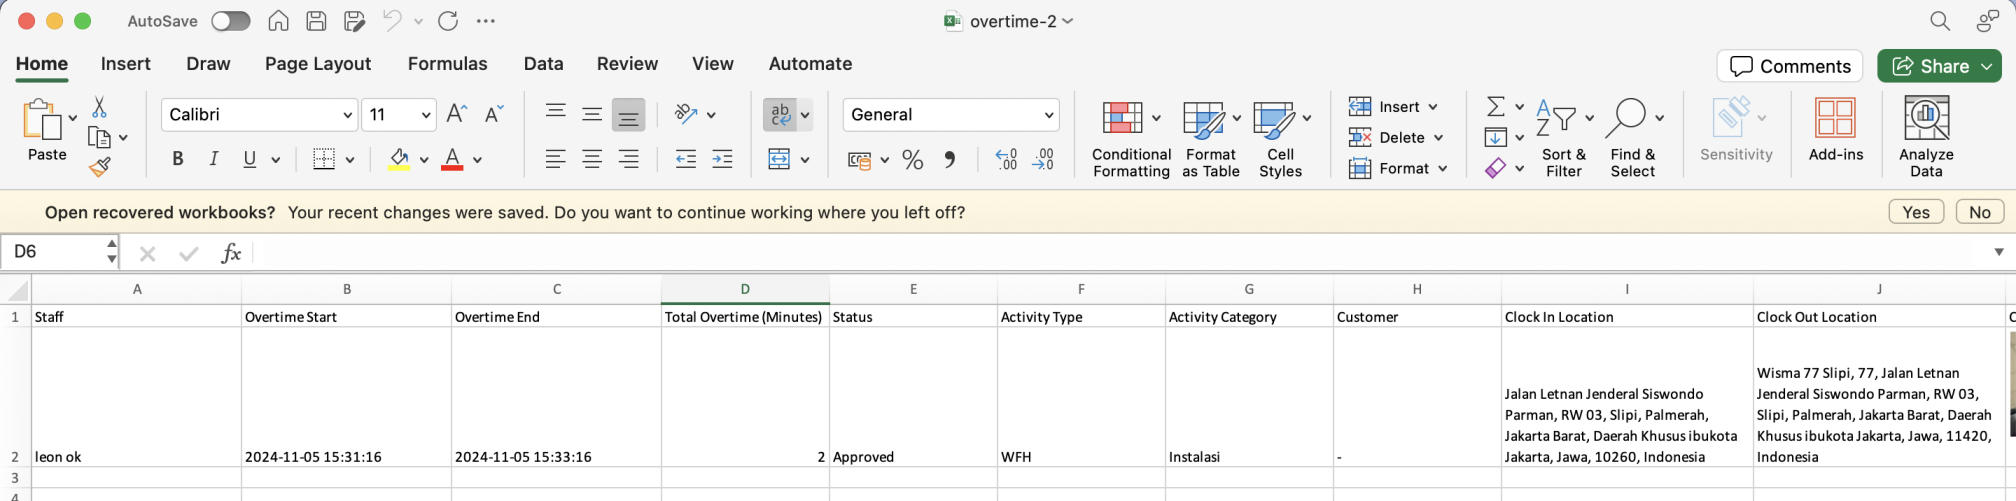
\includegraphics[width=8cm]{Gambar/bab3/user-manual/user-manual-file-excel-riwayat-lembur.png}
    	\caption{\textit{File Excel} Riwayat Lembur}
    	\label{fig:user-manual-file-excel-riwayat-lembur}
        \end{figure}
        \FloatBarrier
    \end{enumerate}
    

    \item Mengakses Halaman \textit{Reject} Lembur\label{item:mengakses-halaman-reject}
    \begin{enumerate}
        \item Melakukan \textit{login} pada aplikasi presensi \textit{online} yang terdapat pada \textbf{Manual \ref{item:melakukan-login}}.
        \item Menekan tombol "\textit{Reject}" pada \textit{navigation bar} yang terletak di paling atas. \textbf{\ref{fig:user-manual-tombol-reject-pada-navigation-bar}} menunjukkan tombol \textit{"Reject"} pada \textit{navigation bar}.
        \begin{figure}[!htbp]
    	\centering
    	
\includegraphics[width=8cm]{Gambar/bab3/user-manual/user-manual-navbar-reject.png}
    	\caption{Tombol \textit{Reject} Pada \textit{Navigation Bar}}
    	\label{fig:user-manual-tombol-reject-pada-navigation-bar}
        \end{figure}
        \FloatBarrier
        \item Sistem akan menampilkan halaman \textit{reject} lembur. \textbf{\ref{fig:user-manual-halaman-reject-lembur}} menunjukkan tampilan halaman \textit{reject lembur}.
        \begin{figure}[!htbp]
    	\centering
    	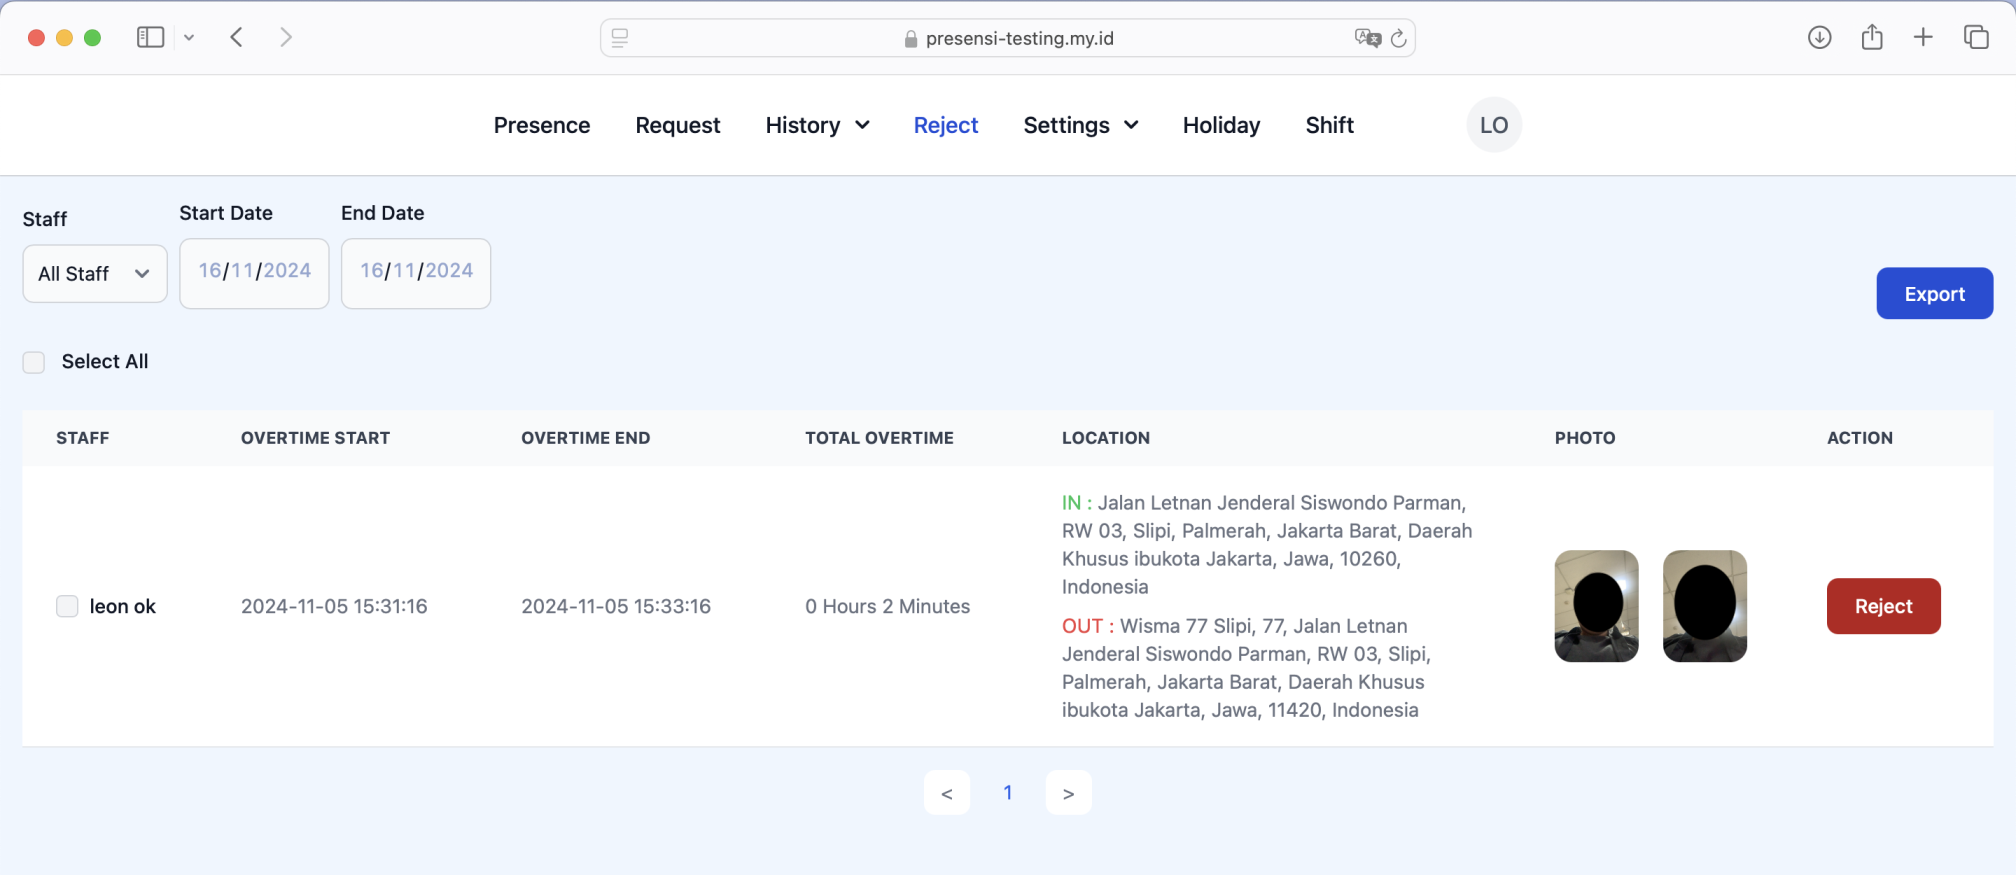
\includegraphics[width=8cm]{Gambar/bab3/user-manual/user-manual-halaman-reject-lembur.png}
    	\caption{Halaman \textit{Reject} Lembur}
    	\label{fig:user-manual-halaman-reject-lembur}
        \end{figure}
        \FloatBarrier
    \end{enumerate}

    \item Melakukan \textit{Reject} Satu Data Lembur
    \begin{enumerate}
        \item Membuka halaman \textit{reject} lembur yang terdapat pada \textbf{Manual \ref{item:mengakses-halaman-reject}}.
        \item Menekan tombol \textit{"Reject"} pada salah satu data lembur dan melakukan konfirmasi. \textbf{\ref{fig:user-manual-tombol-reject-data-lembur}} menunjukkan tombol \textit{"Reject"} pada salah satu data lembur.
        \begin{figure}[!htbp]
    	\centering
    	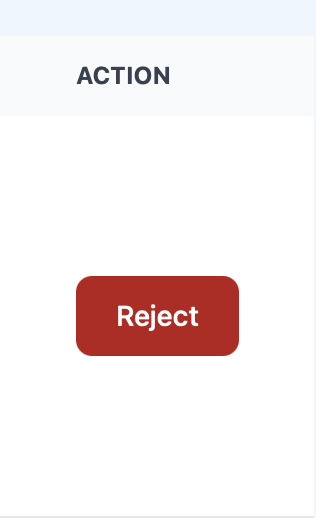
\includegraphics[width=5cm]{Gambar/bab3/user-manual/user-manual-tombol-reject-satu-data-lembur.png}
    	\caption{Tombol \textit{Reject} Pada Data Lembur}
    	\label{fig:user-manual-tombol-reject-data-lembur}
        \end{figure}
        \FloatBarrier
    \end{enumerate}

    \item Melakukan \textit{"Reject"} Lebih Dari Satu Data Lembur
    \begin{enumerate}
        \item Membuka halaman \textit{reject} lembur yang terdapat pada \textbf{Manual \ref{item:mengakses-halaman-reject}}.
        \item Melakukan centang pada \textit{checkbox} data lembur yang akan di-\textit{reject}. \textbf{\ref{fig:user-manual-checkbox-data-lembur}} menunjukkan \textit{checkbox} pada salah satu data lembur.
        \begin{figure}[!htbp]
    	\centering
    	
\includegraphics[width=8cm]{Gambar/bab3/user-manual/user-manual-checkbox-reject-data-lembur.png}
    	\caption{\textit{Checkbox} Data Lembur}
    	\label{fig:user-manual-checkbox-data-lembur}
        \end{figure}
        \FloatBarrier
        \item Setelah memilih \textit{checkbox}, maka akan muncul tombol "\textit{Reject Selected}" untuk me-\textit{reject} seluruh data lembur yang dipilih. \textbf{\ref{fig:user-manual-tombol-reject-selected}} menunjukkan tombol \textit{"Reject Selected"} pada halaman \textit{reject} lembur.
        \begin{figure}[!htbp]
    	\centering
    	
\includegraphics[width=8cm]{Gambar/bab3/user-manual/user-manual-tombol-reject-selected.png}
    	\caption{Tombol \textit{Reject Selected}}
    	\label{fig:user-manual-tombol-reject-selected}
        \end{figure}
        \FloatBarrier
    \end{enumerate}

    \item Melakukan \textit{Export} Data Lembur Pada Halaman \textit{Reject} Lembur
    \begin{enumerate}
        \item Membuka halaman \textit{reject} lembur yang terdapat pada \textbf{Manual \ref{item:mengakses-halaman-reject}}.
        \item Menekan tombol \textit{"Export"} yang terdapat pada halaman \textit{reject} lembur. \textbf{\ref{fig:user-manual-tombol-export-pada-reject-lembur}} menunjukkan tombol "\textit{Export}" pada halaman \textit{reject} lembur.
        \begin{figure}[!htbp]
    	\centering
    	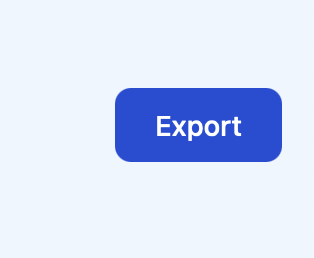
\includegraphics[width=8cm]{Gambar/bab3/user-manual/user-manual-tombol-export-reject-lembur.png}
    	\caption{Tombol \textit{Export} Pada \textit{Reject} Lembur}
    	\label{fig:user-manual-tombol-export-pada-reject-lembur}
        \end{figure}
        \FloatBarrier
        \item Sistem akan otomatis mengunduh \textit{file Excel} yang berisi data lembur dengan status tidak ter-\textit{reject}. \textbf{\ref{fig:user-manual-file-excel-reject-lembur}} menunjukkan \textit{file Excel} yang berisi data lembur yang tidak ter-\textit{reject}.
        \begin{figure}[!htbp]
    	\centering
    	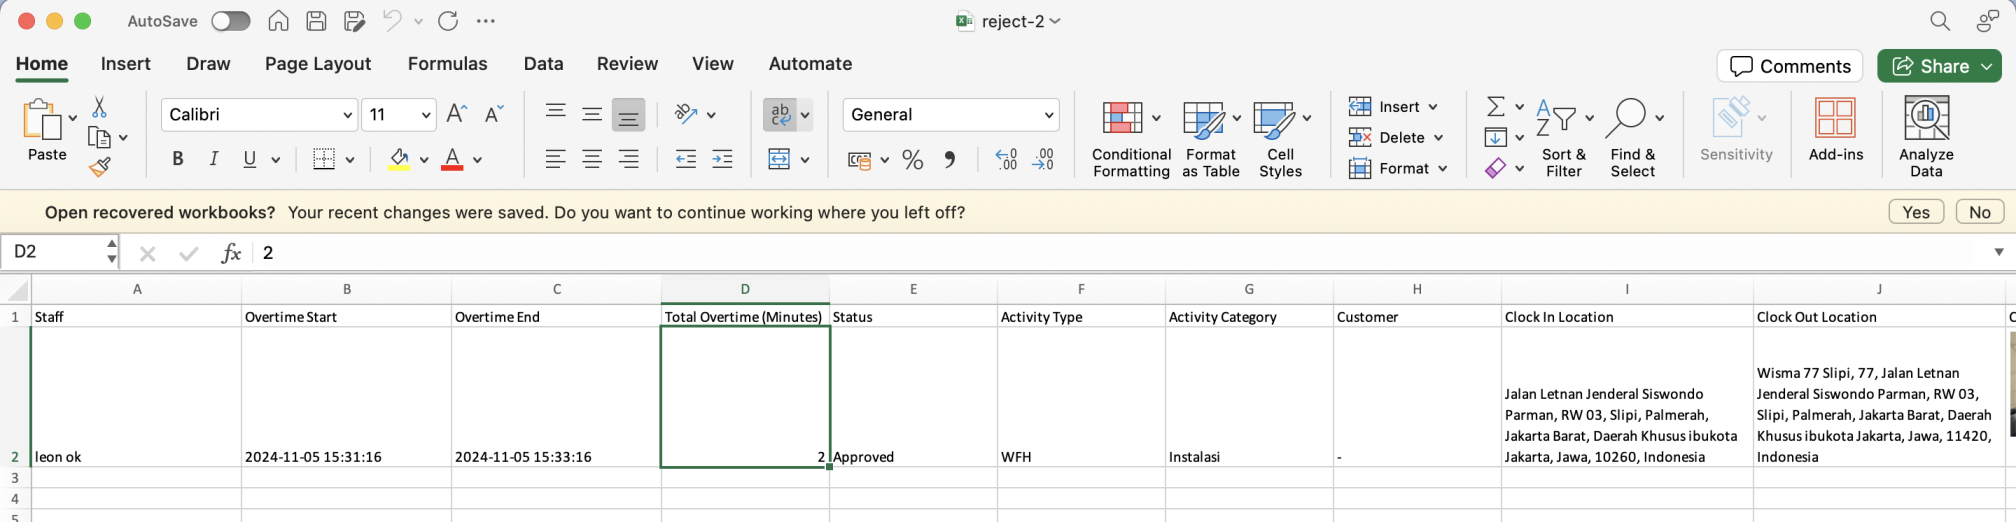
\includegraphics[width=8cm]{Gambar/bab3/user-manual/user-manual-file-excel-reject-lembur.png}
    	\caption{\textit{File Excel Reject} Lembur}
    	\label{fig:user-manual-file-excel-reject-lembur}
        \end{figure}
        \FloatBarrier
    \end{enumerate}

    \item Mengakses Halaman Pengaturan \textit{User}\label{item:mengakses-halaman-pengaturan-user}
    \begin{enumerate}
        \item Melakukan \textit{login} pada aplikasi presensi \textit{online} yang terdapat pada \textbf{Manual \ref{item:melakukan-login}}.
        \item Menekan tombol "\textit{Settings}" pada \textit{navigation bar} yang terletak di paling atas, kemudian tekan tombol "\textit{User}". \textbf{\ref{fig:user-manual-tombol-pengaturan-user-navigation-bar}} menunjukkan tombol \textit{"User"} pada \textit{navigation bar}.
        \begin{figure}[!htbp]
    	\centering
    	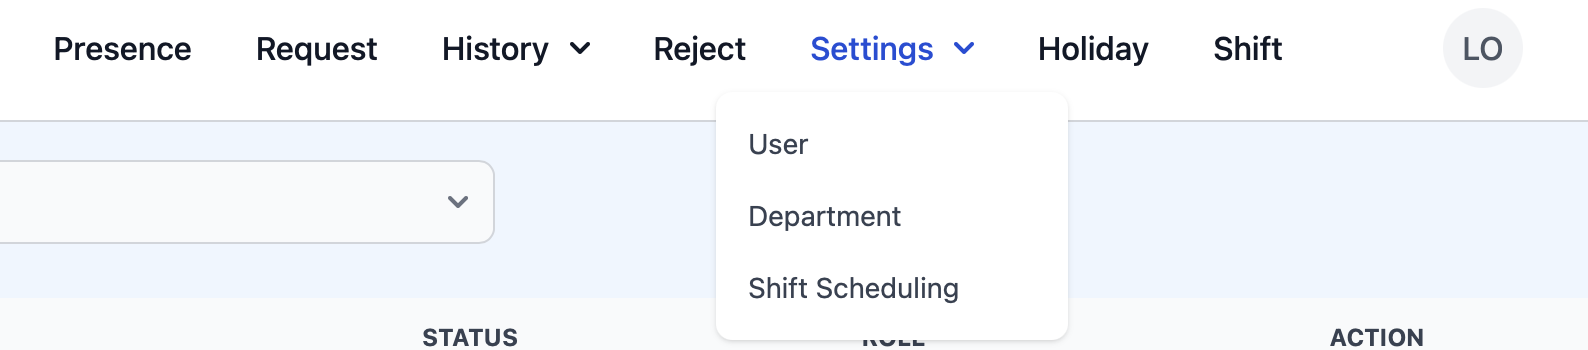
\includegraphics[width=8cm]{Gambar/bab3/user-manual/user-manual-navbar-user.png}
    	\caption{Tombol Pengaturan \textit{User} Pada \textit{Navigation Bar}}
    	\label{fig:user-manual-tombol-pengaturan-user-navigation-bar}
        \end{figure}
        \FloatBarrier
        \item Sistem akan menampilkan data \textit{user} pada halaman pengaturan \textit{user}. \textbf{\ref{fig:user-manual-halaman-pengaturan-user}} menunjukkan halaman pengaturan \textit{user}.
        \begin{figure}[!htbp]
    	\centering
    	\includegraphics[width=8cm]{Gambar/bab3/user-manual/user-manual-halaman-user.png}
    	\caption{Halaman Pengaturan \textit{User}}
    	\label{fig:user-manual-halaman-pengaturan-user}
        \end{figure}
        \FloatBarrier
    \end{enumerate}

    \item Mengubah Data \textit{User}
    \begin{enumerate}
        \item Membuka halaman pengaturan \textit{user} yang terdapat pada \textbf{Manual \ref{item:mengakses-halaman-pengaturan-user}}. \textbf{\ref{fig:user-manual-tombol-edit-pada-data-user}} menunjukkan tombol "\textit{Edit}" pada data \textit{user}.
        \item Menekan tombol \textit{"Edit"} pada salah satu data \textit{user}.
        \begin{figure}[!htbp]
    	\centering
    	\includegraphics[width=8cm]{Gambar/bab3/user-manual/user-manual-tombol-edit-user.png}
    	\caption{Tombol \textit{Edit} Pada Data \textit{User}}
    	\label{fig:user-manual-tombol-edit-pada-data-user}
        \end{figure}
        \FloatBarrier
        \item Mengubah data \textit{user} melalui \textit{input form} pada modal \textit{edit user}, kemudian tekan tombol "\textit{Save Changes}" untuk menyimpan perubahan data. \textbf{\ref{fig:user-manual-modal-edit-user}} menunjukkan modal \textit{edit user}.
        \begin{figure}[!htbp]
    	\centering
    	\includegraphics[width=8cm]{Gambar/bab3/user-manual/user-manual-modal-edit-user.png}
    	\caption{Modal \textit{Edit} \textit{User}}
    	\label{fig:user-manual-modal-edit-user}
        \end{figure}
        \FloatBarrier
    \end{enumerate}

    \item Menghapus Data \textit{User}
    \begin{enumerate}
        \item Membuka halaman pengaturan \textit{user} yang terdapat pada \textbf{Manual \ref{item:mengakses-halaman-pengaturan-user}}.
        \item Menekan tombol "\textit{Delete}" pada salah satu data \textit{user} dan lakukan konfirmasi penghapusan. \textbf{\ref{fig:user-manual-tombol-delete-user}} menunjukkan tombol "\textit{Delete}" untuk menghapus data \textit{user}.
        \begin{figure}[!htbp]
    	\centering
    	\includegraphics[width=8cm]{Gambar/bab3/user-manual/user-manual-tombol-delete-user.png}
    	\caption{Tombol \textit{Delete User}}
    	\label{fig:user-manual-tombol-delete-user}
        \end{figure}
        \FloatBarrier
    \end{enumerate}

    \item Mengakses Halaman \textit{Department}\label{item:mengakses-department}
    \begin{enumerate}
        \item Melakukan \textit{login} pada aplikasi presensi \textit{online} yang terdapat pada \textbf{Manual \ref{item:melakukan-login}}.
        \item Menekan tombol "\textit{Settings}" pada \textit{navigation bar} yang terletak di paling atas, kemudian tekan tombol "\textit{Department}". \textbf{\ref{fig:user-manual-tombol-pengaturan-department-navigation-bar}} menunjukkan tombol \textit{"Department"} pada \textit{navigation bar}.
        \begin{figure}[!htbp]
    	\centering
    	\includegraphics[width=8cm]{Gambar/bab3/user-manual/user-manual-navbar-department.png}
    	\caption{Tombol Pengaturan \textit{Department} Pada \textit{Navigation Bar}}
    	\label{fig:user-manual-tombol-pengaturan-department-navigation-bar}
        \end{figure}
        \FloatBarrier
        \item Sistem akan menampilkan data \textit{department} pada halaman pengaturan \textit{department}. \textbf{\ref{fig:user-manual-halaman-pengaturan-department}} menunjukkan halaman pengaturan \textit{department}.
        \begin{figure}[!htbp]
    	\centering
    	\includegraphics[width=8cm]{Gambar/bab3/user-manual/user-manual-halaman-department.png}
    	\caption{Halaman Pengaturan \textit{Department}}
    	\label{fig:user-manual-halaman-pengaturan-department}
        \end{figure}
        \FloatBarrier
    \end{enumerate}

    \item Menambah \textit{Department}
    \begin{enumerate}
        \item Membuka halaman pengaturan \textit{department} yang terdapat pada \textbf{Manual \ref{item:mengakses-department}}.
        \item Menekan tombol "\textit{Create Department}" pada halaman pengaturan \textit{department}. \textbf{\ref{fig:user-manual-tombol-create-new-department}} menunjukkan tombol "\textit{Create Department}" pada halaman pengaturan \textit{department}.
        \begin{figure}[!htbp]
    	\centering
    	\includegraphics[width=8cm]{Gambar/bab3/user-manual/user-manual-tombol-create-new-department.png}
    	\caption{Tombol \textit{Create Department}}
    	\label{fig:user-manual-tombol-create-new-department}
        \end{figure}
        \FloatBarrier

        \item Mengisi seluruh \textit{input form} pada modal \textit{create new department}, kemudian tekan tombol "\textit{Create New Department}" untuk menyimpan data \textit{department} baru. \textbf{\ref{fig:user-manual-modal-create-new-department}} menunjukkan modal \textit{create new department}.
        \begin{figure}[!htbp]
    	\centering
    	\includegraphics[width=8cm]{Gambar/bab3/user-manual/user-manual-modal-create-new-department.png}
    	\caption{Modal \textit{Create New Department}}
    	\label{fig:user-manual-modal-create-new-department}
        \end{figure}
        \FloatBarrier
    \end{enumerate}

    \item Mengubah \textit{Department}
    \begin{enumerate}
        \item Membuka halaman pengaturan \textit{department} yang terdapat pada \textbf{Manual \ref{item:mengakses-department}}.
        \item Menekan tombol "\textit{Edit}" salah satu data \textit{department} pada halaman pengaturan \textit{department}. \textbf{\ref{fig:user-manual-tombol-edit-department}} menunjukkan tombol "\textit{Edit}" pada halaman pengaturan \textit{department}.
        \begin{figure}[!htbp]
    	\centering
    	\includegraphics[width=8cm]{Gambar/bab3/user-manual/user-manual-tombol-edit-department.png}
    	\caption{Tombol \textit{Edit} Department}
    	\label{fig:user-manual-tombol-edit-department}
        \end{figure}
        \FloatBarrier

        \item Mengubah seluruh \textit{input form} pada modal \textit{edit department}, kemudian tekan tombol "\textit{Save Changes}" untuk menyimpan data \textit{department}. \textbf{\ref{fig:user-manual-modal-edit-department}} menunjukkan modal \textit{edit department}.
        \begin{figure}[!htbp]
    	\centering
    	\includegraphics[width=8cm]{Gambar/bab3/user-manual/user-manual-modal-edit-department.png}
    	\caption{Modal \textit{Edit Department}}
    	\label{fig:user-manual-modal-edit-department}
        \end{figure}
        \FloatBarrier
    \end{enumerate}

    \item Menghapus Data \textit{Department}
    \begin{enumerate}
        \item Membuka halaman pengaturan \textit{department} yang terdapat pada \textbf{Manual \ref{item:mengakses-department}}.
        \item Menekan tombol "\textit{Delete}" pada salah satu data \textit{department} dan lakukan konfirmasi penghapusan. \textbf{\ref{fig:user-manual-tombol-delete-department}} menunjukkan tombol "\textit{Delete}" untuk menghapus data \textit{department}.
        \begin{figure}[!htbp]
    	\centering
    	\includegraphics[width=8cm]{Gambar/bab3/user-manual/user-manual-tombol-delete-department.png}
    	\caption{Tombol \textit{Delete Department}}
    	\label{fig:user-manual-tombol-delete-department}
        \end{figure}
        \FloatBarrier
    \end{enumerate}

    \item Mengakses Halaman Penjadwalan \textit{Shift}\label{item:mengakses-shift-scheduling}
    \begin{enumerate}
        \item Melakukan \textit{login} pada aplikasi presensi \textit{online} yang terdapat pada \textbf{Manual \ref{item:melakukan-login}}.
        \item Menekan tombol "\textit{Settings}" pada \textit{navigation bar} yang terletak di paling atas, kemudian tekan tombol "\textit{Shift Scheduling}". \textbf{\ref{fig:user-manual-tombol-pengaturan-shift-scheduling-navigation-bar}} menunjukkan tombol \textit{"Shift Scheduling"} pada \textit{navigation bar}.
        \begin{figure}[!htbp]
    	\centering
    	\includegraphics[width=8cm]{Gambar/bab3/user-manual/user-manual-navbar-shift-scheduling.png}
    	\caption{Tombol Pengaturan \textit{Shift Scheduling} Pada \textit{Navigation Bar}}
    	\label{fig:user-manual-tombol-pengaturan-shift-scheduling-navigation-bar}
        \end{figure}
        \FloatBarrier
        \item Sistem akan menampilkan data penjadwalan \textit{shift} pada halaman pengaturan \textit{shift scheduling}. \textbf{\ref{fig:user-manual-halaman-pengaturan-shift-scheduling}} menunjukkan halaman pengaturan \textit{shift scheduling}.
        \begin{figure}[!htbp]
    	\centering
    	\includegraphics[width=8cm]{Gambar/bab3/user-manual/user-manual-halaman-shift-scheduling.png}
    	\caption{Halaman Pengaturan \textit{Shift Scheduling}}
    	\label{fig:user-manual-halaman-pengaturan-shift-scheduling}
        \end{figure}
        \FloatBarrier
    \end{enumerate}

    \item Menambah Data Penjadwalan \textit{Shift}
    \begin{enumerate}
        \item Membuka halaman \textit{shift scheduling} yang terdapat pada \textbf{Manual \ref{item:mengakses-shift-scheduling}}.
        \item Menekan tombol "\textit{Create New Schedule}" pada halaman pengaturan \textit{shift scheduling}. \textbf{\ref{fig:user-manual-tombol-create-new-schedule}} menunjukkan tombol "\textit{Create New Schedule}" pada halaman pengaturan \textit{shift scheduling}.
        \begin{figure}[!htbp]
    	\centering
    	\includegraphics[width=8cm]{Gambar/bab3/user-manual/user-manual-tombol-create-new-schedule.png}
    	\caption{Tombol \textit{Create New Schedule}}
    	\label{fig:user-manual-tombol-create-new-schedule}
        \end{figure}
        \FloatBarrier

        \item Mengisi seluruh \textit{input form} pada modal \textit{create new schedule}, kemudian tekan tombol "\textit{Create New Schedule}" untuk menyimpan data penjadwalan \textit{shift} baru. \textbf{\ref{fig:user-manual-modal-create-new-schedule}} menunjukkan modal \textit{create new schedule}.
        \begin{figure}[!htbp]
    	\centering
    	\includegraphics[width=8cm]{Gambar/bab3/user-manual/user-manual-modal-create-new-schedule.png}
    	\caption{Modal \textit{Create New Schedule}}
    	\label{fig:user-manual-modal-create-new-schedule}
        \end{figure}
        \FloatBarrier
    \end{enumerate}

    \item Mengubah Data Penjadwalan \textit{Shift}
    \begin{enumerate}
        \item Membuka halaman \textit{shift scheduling} yang terdapat pada \textbf{Manual \ref{item:mengakses-shift-scheduling}}.
        \item Menekan tombol "\textit{Edit}" salah satu data \textit{shift scheduling} pada halaman pengaturan \textit{shift scheduling}. \textbf{\ref{fig:user-manual-tombol-edit-schedule}} menunjukkan tombol "\textit{Edit}" pada halaman pengaturan \textit{shift scheduling}.
        \begin{figure}[!htbp]
    	\centering
    	\includegraphics[width=8cm]{Gambar/bab3/user-manual/user-manual-tombol-edit-schedule.png}
    	\caption{Tombol \textit{Edit Schedule}}
    	\label{fig:user-manual-tombol-edit-schedule}
        \end{figure}
        \FloatBarrier

        \item Mengubah seluruh \textit{input form} pada modal \textit{edit schedule}, kemudian tekan tombol "\textit{Edit Schedule}" untuk menyimpan data \textit{shift scheduling}. \textbf{\ref{fig:user-manual-modal-edit-schedule}} menunjukkan modal \textit{edit schedule}.
        \begin{figure}[!htbp]
    	\centering
    	\includegraphics[width=8cm]{Gambar/bab3/user-manual/user-manual-modal-edit-schedule.png}
    	\caption{Modal \textit{Edit Schedule}}
    	\label{fig:user-manual-modal-edit-schedule}
        \end{figure}
        \FloatBarrier
    \end{enumerate}

    \item Menghapus Data Penjadwalan \textit{Shift}
    \begin{enumerate}
        \item Membuka halaman \textit{shift scheduling} yang terdapat pada \textbf{Manual \ref{item:mengakses-shift-scheduling}}.
        \item Menekan tombol "\textit{Delete}" pada salah satu data \textit{shift scheduling} dan lakukan konfirmasi penghapusan. \textbf{\ref{fig:user-manual-tombol-delete-shift-scheduling}} menunjukkan tombol "\textit{Delete}" untuk menghapus data \textit{shift scheduling}.
        \begin{figure}[!htbp]
    	\centering
    	\includegraphics[width=8cm]{Gambar/bab3/user-manual/user-manual-tombol-delete-schedule.png}
    	\caption{Tombol \textit{Delete Shift Scheduling}}
    	\label{fig:user-manual-tombol-delete-shift-scheduling}
        \end{figure}
        \FloatBarrier
    \end{enumerate}

    \item Melakukan \textit{Export} Data Penjadwalan \textit{Shift}\label{item:export-shift-scheduling}
    \begin{enumerate}
        \item Membuka halaman \textit{shift scheduling} yang terdapat pada \textbf{Manual \ref{item:mengakses-shift-scheduling}}.
        \item Menekan tombol "\textit{Export Schedule}" pada halaman \textit{shift scheduling}. \textbf{\ref{fig:user-manual-tombol-export-shift-scheduling}} menunjukkan tombol \textit{"Export Schedule"} untuk men-\textit{download} data \textit{shift scheduling}.
        \begin{figure}[!htbp]
    	\centering
    	\includegraphics[width=8cm]{Gambar/bab3/user-manual/user-manual-tombol-export-shift-scheduling.png}
    	\caption{Tombol \textit{Export Shift Scheduling}}
    	\label{fig:user-manual-tombol-export-shift-scheduling}
        \end{figure}
        \FloatBarrier
        \item Sistem akan otomatis mengunduh \textit{file Excel} yang berisi seluruh data \textit{shift scheduling}. \textbf{\ref{fig:user-manual-file-excel-shift-scheduling}} menunjukkan \textit{file Excel} yang berisi seluruh data \textit{shift scheduling}.
        \begin{figure}[!htbp]
    	\centering
    	\includegraphics[width=8cm]{Gambar/bab3/user-manual/user-manual-file-excel-shift-scheduling.png}
    	\caption{\textit{File Excel} \textit{Shift Scheduling}}
    	\label{fig:user-manual-file-excel-shift-scheduling}
        \end{figure}
        \FloatBarrier
    \end{enumerate}

    \item Melakukan \textit{Import} Penjadwalan \textit{Shift}
    \begin{enumerate}
        \item Membuka halaman \textit{shift scheduling} yang terdapat pada \textbf{Manual \ref{item:mengakses-shift-scheduling}}.
        \item Menekan tombol "\textit{Import Schedule}" pada halaman \textit{shift scheduling}. \textbf{\ref{fig:user-manual-tombol-import-shift-scheduling}} menunjukkan tombol \textit{"Import Schedule"}.
        \begin{figure}[!htbp]
    	\centering
    	\includegraphics[width=8cm]{Gambar/bab3/user-manual/user-manual-tombol-import-shift-scheduling.png}
    	\caption{Tombol \textit{Import Shift Scheduling}}
    	\label{fig:user-manual-tombol-import-shift-scheduling}
        \end{figure}
        \FloatBarrier
        \item Meng-\textit{upload} dan mengubah isi \textit{file Excel} yang telah diunduh dari \textbf{Manual \ref{item:export-shift-scheduling}}, kemudian tekan tombol "\textit{Import Now}" untuk me-\textit{replace} seluruh \textit{shift scheduling}. \textbf{\ref{fig:user-manual-modal-import-shift-scheduling}} menunjukkan modal \textit{import shift scheduling}.
        \begin{figure}[!htbp]
    	\centering
    	\includegraphics[width=8cm]{Gambar/bab3/user-manual/user-manual-modal-import-shift-scheduling.png}
    	\caption{Modal \textit{Import Shift Scheduling}}
    	\label{fig:user-manual-modal-import-shift-scheduling}
        \end{figure}
        \FloatBarrier
    \end{enumerate}


    \item Mengakses Halaman Jenis Libur Perusahaan\label{item:mengakses-jenis-libur-perusahaan}
    \begin{enumerate}
        \item Melakukan \textit{login} pada aplikasi presensi \textit{online} yang terdapat pada \textbf{Manual \ref{item:melakukan-login}}.
        \item Menekan tombol "\textit{Holiday}" pada \textit{navigation bar} yang terletak di paling atas. \textbf{\ref{fig:user-manual-tombol-holiday-navigation-bar}} menunjukkan tombol \textit{"Holiday"} pada \textit{navigation bar}.
        \begin{figure}[!htbp]
    	\centering
    	\includegraphics[width=8cm]{Gambar/bab3/user-manual/user-manual-navbar-holiday.png}
    	\caption{Tombol \textit{Holiday} Pada \textit{Navigation Bar}}
    	\label{fig:user-manual-tombol-holiday-navigation-bar}
        \end{figure}
        \FloatBarrier
        \item Sistem akan menampilkan data jenis libur perusahaan pada halaman \textit{holiday}. \textbf{\ref{fig:user-manual-halaman-holiday}} menunjukkan halaman \textit{holiday}.
        \begin{figure}[!htbp]
    	\centering
    	\includegraphics[width=8cm]{Gambar/bab3/user-manual/user-manual-halaman-jenis-libur-perusahaan.png}
    	\caption{Halaman \textit{Holiday}}
    	\label{fig:user-manual-halaman-holiday}
        \end{figure}
        \FloatBarrier
    \end{enumerate}

    \item Menambah Jenis Libur Perusahaan
    \begin{enumerate}
        \item Membuka halaman jenis libur perusahaan yang terdapat pada \textbf{Manual \ref{item:mengakses-jenis-libur-perusahaan}}.
        \item Menekan tombol "\textit{Create New Holiday}" pada halaman \textit{holiday}. \textbf{\ref{fig:user-manual-tombol-create-new-holiday}} menunjukkan tombol "\textit{Create New Holiday}" pada halaman \textit{holiday}.
        \begin{figure}[!htbp]
    	\centering
    	\includegraphics[width=8cm]{Gambar/bab3/user-manual/user-manual-tombol-create-new-holiday.png}
    	\caption{Tombol "\textit{Create New Holiday}"}
    	\label{fig:user-manual-tombol-create-new-holiday}
        \end{figure}
        \FloatBarrier

        \item Mengisi seluruh \textit{input form} pada modal \textit{create new holiday}, kemudian tekan tombol "\textit{Create New Holiday Category}" untuk menyimpan data jenis libur perusahaan baru. \textbf{\ref{fig:user-manual-modal-create-new-holiday}} menunjukkan modal \textit{create new holiday}.
        \begin{figure}[!htbp]
    	\centering
    	\includegraphics[width=8cm]{Gambar/bab3/user-manual/user-manual-modal-create-new-holiday.png}
    	\caption{Modal \textit{Create New Holiday}}
    	\label{fig:user-manual-modal-create-new-holiday}
        \end{figure}
        \FloatBarrier
    \end{enumerate}

    \item Menghapus Data Jenis Libur Perusahaan
    \begin{enumerate}
        \item Membuka halaman jenis libur perusahaan yang terdapat pada \textbf{Manual \ref{item:mengakses-jenis-libur-perusahaan}}.
        \item Menekan tombol "\textit{Delete}" pada salah satu data \textit{holiday} dan lakukan konfirmasi penghapusan. \textbf{\ref{fig:user-manual-tombol-delete-holiday}} menunjukkan tombol "\textit{Delete}" untuk menghapus data \textit{holiday}.
        \begin{figure}[!htbp]
    	\centering
    	\includegraphics[width=8cm]{Gambar/bab3/user-manual/user-manual-tombol-delete-holiday.png}
    	\caption{Tombol \textit{Delete Holiday}}
    	\label{fig:user-manual-tombol-delete-holiday}
        \end{figure}
        \FloatBarrier
    \end{enumerate}

    \item Mengakses Halaman Hari Pada Jenis Libur Perusahaan\label{item:mengakses-halaman-hari-jenis-libur-perusahaan}
    \begin{enumerate}
        \item Membuka halaman jenis libur perusahaan yang terdapat pada \textbf{Manual \ref{item:mengakses-jenis-libur-perusahaan}}.
        \item Menekan tombol "\textit{Edit}" salah satu data \textit{holiday} pada halaman \textit{holiday}. \textbf{\ref{fig:user-manual-tombol-edit-holiday}} menunjukkan tombol "\textit{Edit}" pada halaman \textit{holiday}.
        \begin{figure}[!htbp]
    	\centering
    	\includegraphics[width=8cm]{Gambar/bab3/user-manual/user-manual-tombol-edit-holiday.png}
    	\caption{Tombol \textit{Edit} \textit{Holiday}}
    	\label{fig:user-manual-tombol-edit-holiday}
        \end{figure}
        \FloatBarrier

        \item Sistem akan menampilkan halaman data hari pada jenis perusahaan yang dipilih. \textbf{\ref{fig:user-manual-halaman-hari-jenis-libur-perusahaan}} menunjukkan halaman hari pada jenis libur perusahaan.
        \begin{figure}[!htbp]
    	\centering
    	\includegraphics[width=8cm]{Gambar/bab3/user-manual/user-manual-halaman-hari-jenis-libur-perusahaan.png}
    	\caption{Halaman Hari Pada Jenis Libur Perusahaan}
    	\label{fig:user-manual-halaman-hari-jenis-libur-perusahaan}
        \end{figure}
        \FloatBarrier
    \end{enumerate}

    \item Menambah Hari Pada Jenis Libur Perusahaan
    \begin{enumerate}
        \item Membuka halaman pengaturan \textit{department} yang terdapat pada \textbf{Manual \ref{item:mengakses-halaman-hari-jenis-libur-perusahaan}}.
        \item Menekan tombol "\textit{Create New Holiday}" pada halaman hari pada jenis libur perusahaan. \textbf{\ref{fig:user-manual-tombol-tambah-hari-jenis-libur-perusahaan}} menunjukkan tombol "\textit{Create New Holiday}" pada halaman hari pada jenis libur perusahaan.
        \begin{figure}[!htbp]
    	\centering
    	\includegraphics[width=8cm]{Gambar/bab3/user-manual/user-manual-tombol-tambah-hari-jenis-libur-perusahaan.png}
    	\caption{Tombol "\textit{Create New Holiday}"}
    	\label{fig:user-manual-tombol-tambah-hari-jenis-libur-perusahaan}
        \end{figure}
        \FloatBarrier

        \item Mengisi seluruh \textit{input form} pada modal \textit{create new holiday}, kemudian tekan tombol "\textit{Create New Holiday Category}" untuk menyimpan data hari pada jenis libur perusahaan. \textbf{\ref{fig:user-manual-modal-tambah-hari-pada-jenis-libur-perusahaan}} menunjukkan modal \textit{create new holiday}.
        \begin{figure}[!htbp]
    	\centering
    	\includegraphics[width=8cm]{Gambar/bab3/user-manual/user-manual-modal-tambah-hari-jenis-libur-perusahaan.png}
    	\caption{Modal \textit{Create New Holiday}}
    	\label{fig:user-manual-modal-tambah-hari-pada-jenis-libur-perusahaan}
        \end{figure}
        \FloatBarrier
    \end{enumerate}


    \item Mengubah Data Hari Pada Jenis Libur Perusahaan
    \begin{enumerate}
        \item Membuka halaman hari pada jenis libur perusahaan yang terdapat pada \textbf{Manual \ref{item:mengakses-halaman-hari-jenis-libur-perusahaan}}.
        \item Menekan tombol "\textit{Edit}" salah satu data hari pada jenis libur perusahaan pada halaman hari jenis libur perusahaan. \textbf{\ref{fig:user-manual-tombol-edit-hari-jenis-libur-perusahaan}} menunjukkan tombol "\textit{Edit}" pada halaman hari jenis libur perusahaan.
        \begin{figure}[!htbp]
    	\centering
    	\includegraphics[width=8cm]{Gambar/bab3/user-manual/user-manual-tombol-edit-hari-jenis-libur-perusahaan.png}
    	\caption{Tombol \textit{Edit} Pada Jenis Libur Perusahaan}
    	\label{fig:user-manual-tombol-edit-hari-jenis-libur-perusahaan}
        \end{figure}
        \FloatBarrier

        \item Mengubah seluruh \textit{input form} pada modal \textit{edit} hari jenis libur perusahaan, kemudian tekan tombol "\textit{Save Changes}" untuk menyimpan data hari pada jenis libur perusahaan. \textbf{\ref{fig:user-manual-modal-edit-hari-jenis-libur-perusahaan}} menunjukkan modal \textit{edit} hari jenis libur perusahaan.
        \begin{figure}[!htbp]
    	\centering
    	\includegraphics[width=8cm]{Gambar/bab3/user-manual/user-manual-modal-edit-hari-jenis-libur-perusahaan.png}
    	\caption{Modal \textit{Edit} Hari Pada Jenis Libur Perusahaan}
    	\label{fig:user-manual-modal-edit-hari-jenis-libur-perusahaan}
        \end{figure}
        \FloatBarrier
    \end{enumerate}

    \item Menghapus Data Hari Pada Jenis Libur Perusahaan
    \begin{enumerate}
        \item Membuka halaman hari pada jenis libur perusahaan yang terdapat pada \textbf{Manual \ref{item:mengakses-halaman-hari-jenis-libur-perusahaan}}.
        \item Menekan tombol "\textit{Delete}" pada salah satu data hari pada jenis libur perusahaan dan lakukan konfirmasi penghapusan. \textbf{\ref{fig:user-manual-tombol-delete-hari-jenis-libur-perusahaan}} menunjukkan tombol "\textit{Delete}" untuk menghapus data hari pada jenis libur perusahaan.
        \begin{figure}[!htbp]
    	\centering
    	\includegraphics[width=8cm]{Gambar/bab3/user-manual/user-manual-hapus-hari-jenis-libur-perusahaan.png}
    	\caption{Tombol \textit{Delete} Hari Pada Jenis Libur Perusahaan}
    	\label{fig:user-manual-tombol-delete-hari-jenis-libur-perusahaan}
        \end{figure}
        \FloatBarrier
    \end{enumerate}

    \item Mengimpor Hari Libur Nasional Otomatis Pada Jenis Libur Perusahaan
    \begin{enumerate}
        \item Membuka halaman hari pada jenis libur perusahaan yang terdapat pada \textbf{Manual \ref{item:mengakses-halaman-hari-jenis-libur-perusahaan}}.
        \item Menekan tombol "\textit{Import National DayOff}" pada halaman hari jenis libur perusahaan. \textbf{\ref{fig:user-manual-tombol-import-libur-nasional-hari-jenis-libur-perusahaan}} menunjukkan tombol "\textit{Import National DayOff}" untuk mengambil data libur nasional Indonesia secara otomatis.
        \begin{figure}[!htbp]
    	\centering
    	\includegraphics[width=8cm]{Gambar/bab3/user-manual/user-manual-tombol-import-hari-libur-nasional.png}
    	\caption{Tombol \textit{Import} Hari Libur Nasional Pada Jenis Libur Perusahaan}
    	\label{fig:user-manual-tombol-import-libur-nasional-hari-jenis-libur-perusahaan}
        \end{figure}
        \FloatBarrier
        \item Memilih tahun yang akan dicari hari liburnya dan menekan tombol "\textit{Add}" untuk melihat \textit{preview} data libur nasional Indonesia, pilih data yang ingin dimasukkan kemudian tekan tombol "\textit{Import Now}" pada modal \textit{import national DayOff}. \textbf{\ref{fig:user-manual-modal-import-libur-nasional-hari-jenis-libur-perusahaan}} menunjukkan modal \textit{import national DayOff}.
        \begin{figure}[!htbp]
    	\centering
    	\includegraphics[width=8cm]{Gambar/bab3/user-manual/user-manual-modal-import-hari-libur-nasional.png}
    	\caption{Modal \textit{Import} Hari Libur Nasional Pada Jenis Libur Perusahaan}
    	\label{fig:user-manual-modal-import-libur-nasional-hari-jenis-libur-perusahaan}
        \end{figure}
        \FloatBarrier

         \item Sistem akan menampilkan modal untuk memberikan informasi terkait data yang berhasil di\textit{import} dan gagal. \textbf{\ref{fig:user-manual-modal-hasil-import-libur-nasional-hari-jenis-libur-perusahaan}} menunjukkan hasil \textit{import} data hari libur nasional Indonesia.
    \begin{figure}[!htbp]
    	\centering
    	\includegraphics[width=8cm]{Gambar/bab3/user-manual/user-manual-modal-hasil-import-hari-libur-nasional.png}
    	\caption{Modal Hasil \textit{Import} Hari Libur Nasional Pada Jenis Libur Perusahaan}
    	\label{fig:user-manual-modal-hasil-import-libur-nasional-hari-jenis-libur-perusahaan}
        \end{figure}
    \FloatBarrier
    \end{enumerate}

    % BELUM DI INSERT GAMBAR 

    \item Mengakses Halaman Jenis \textit{Shift}\label{item:mengakses-halaman-jenis-shift}
    \begin{enumerate}
        \item Melakukan \textit{login} pada aplikasi presensi \textit{online} yang terdapat pada \textbf{Manual \ref{item:melakukan-login}}.
        \item Menekan tombol "\textit{Shift}" pada \textit{navigation bar} yang terletak di paling atas. \textbf{\ref{fig:user-manual-tombol-shift-pada-navigation-bar}} menunjukkan tombol \textit{"Shift"} pada \textit{navigation bar}.
        \begin{figure}[!htbp]
    	\centering
    	\includegraphics[width=8cm]{Gambar/bab3/user-manual/user-manual-navbar-shift.png}
    	\caption{Tombol \textit{Shift} Pada \textit{Navigation Bar}}
    	\label{fig:user-manual-tombol-shift-pada-navigation-bar}
        \end{figure}
        \FloatBarrier
        \item Sistem akan menampilkan halaman jenis \textit{shift} beserta data jenis \textit{shift}. \textbf{\ref{fig:user-manual-halaman-jenis-shift}} menunjukkan halaman jenis \textit{shift}.
        \begin{figure}[!htbp]
    	\centering
    	\includegraphics[width=8cm]{Gambar/bab3/user-manual/user-manual-halaman-jenis-shift.png}
    	\caption{Halaman Jenis \textit{Shift}}
    	\label{fig:user-manual-halaman-jenis-shift}
        \end{figure}
        \FloatBarrier
    \end{enumerate}

    \item Menambah Jenis \textit{Shift}
    \begin{enumerate}
        \item Membuka halaman jenis libur \textit{shift} yang terdapat pada \textbf{Manual \ref{item:mengakses-halaman-jenis-shift}}.
        \item Menekan tombol "\textit{Create New Shift}" pada halaman jenis \textit{shift}. \textbf{\ref{fig:user-manual-tombol-create-new-shift}} menunjukkan tombol "\textit{Create New Shift}" pada halaman jenis \textit{shift}.
        \begin{figure}[!htbp]
    	\centering
    	\includegraphics[width=8cm]{Gambar/bab3/user-manual/user-manual-tombol-create-new-shift.png}
    	\caption{Tombol \textit{Create New Shift} Pada Halaman Jenis \textit{Shift}}
    	\label{fig:user-manual-tombol-create-new-shift}
        \end{figure}
        \FloatBarrier
        \item Mengisi seluruh \textit{input form} pada modal \textit{create new shift} dan tekan tombol \textit{"Create New Shift"} untuk menyimpan data jenis \textit{shift} baru. \textbf{\ref{fig:user-manual-modal-create-new-shift}} menunjukkan modal \textit{create new shift}.
        \begin{figure}[!htbp]
    	\centering
    	\includegraphics[width=8cm]{Gambar/bab3/user-manual/user-manual-modal-create-new-shift.png}
    	\caption{Modal \textit{Create New Shift} Pada Halaman Jenis \textit{Shift}}
    	\label{fig:user-manual-modal-create-new-shift}
        \end{figure}
        \FloatBarrier
    \end{enumerate}

    \item Menghapus Jenis \textit{Shift}
    \begin{enumerate}
        \item Membuka halaman jenis libur \textit{shift} yang terdapat pada \textbf{Manual \ref{item:mengakses-halaman-jenis-shift}}.
        \item Menekan tombol "\textit{Delete}" pada salah satu data jenis \textit{shift} melalui halaman jenis \textit{shift} dan melakukan konfirmasi. \textbf{\ref{fig:user-manual-tombol-delete-shift}} menunjukkan tombol "\textit{Delete}" pada salah satu data jenis \textit{shift}.
        \begin{figure}[!htbp]
    	\centering
    	\includegraphics[width=5cm]{Gambar/bab3/user-manual/user-manual-tombol-delete-shift.png}
    	\caption{Tombol \textit{Delete} Pada Jenis \textit{Shift}}
    	\label{fig:user-manual-tombol-delete-shift}
        \end{figure}
        \FloatBarrier
    \end{enumerate}

    \item Melakukan \textit{Edit} Jenis \textit{Shift}\label{item:melakukan-edit-jenis-shift}
    \begin{enumerate}
        \item Membuka halaman jenis libur \textit{shift} yang terdapat pada \textbf{Manual \ref{item:mengakses-halaman-jenis-shift}}.
        \item Menekan tombol "\textit{Edit}" pada salah satu data jenis \textit{shift} melalui halaman jenis \textit{shift}. \textbf{\ref{fig:user-manual-tombol-edit-shift}} menunjukkan tombol "\textit{Edit}" pada salah satu data jenis \textit{shift}.
        \begin{figure}[!htbp]
    	\centering
    	\includegraphics[width=5cm]{Gambar/bab3/user-manual/user-manual-tombol-edit-shift.png}
    	\caption{Tombol \textit{Edit} Pada Jenis \textit{Shift}}
    	\label{fig:user-manual-tombol-edit-shift}
        \end{figure}
        \FloatBarrier
        
        \item Mengisi \textit{input form} pada modal \textit{edit shift} dan tekan tombol "\textit{Save Changes}" untuk menyimpan perubahan jenis \textit{shift}. \textbf{\ref{fig:user-manual-tombol-edit-jenis-shift}} menunjukkan modal \textit{edit shift}.
        \begin{figure}[!htbp]
    	\centering
    	\includegraphics[width=8cm]{Gambar/bab3/user-manual/user-manual-modal-edit-shift.png}
    	\caption{Tombol \textit{Edit} Pada Jenis \textit{Shift}}
    	\label{fig:user-manual-tombol-edit-jenis-shift}
        \end{figure}
        \FloatBarrier
    \end{enumerate}

    \item Menambah Hari Pada Jenis \textit{Shift}
    \begin{enumerate}
        \item Mengakses modal \textit{edit} jenis \textit{shift} pada \textbf{Manual \ref{item:melakukan-edit-jenis-shift}}.
        \item Menekan tombol "\textit{Add Day}" pada modal \textit{edit} jenis \textit{shift}. \textbf{\ref{fig:user-manual-tombol-add-shift-day}} menunjukkan tombol \textit{"Add Day"} untuk membuka modal \textit{add shift day}.
        \begin{figure}[!htbp]
    	\centering
    	\includegraphics[width=5cm]{Gambar/bab3/user-manual/user-manual-tombol-add-shiftday.png}
    	\caption{Tombol \textit{Add Day} Pada Jenis \textit{Shift}}
    	\label{fig:user-manual-tombol-add-shift-day}
        \end{figure}
        \FloatBarrier
        \item Mengisi seluruh \textit{input form} pada \textit{add shift day} dan menekan tombol "\textit{Add Day}" untuk menyimpan hari baru pada jenis \textit{shift}. \textbf{\ref{fig:user-manual-modal-add-shift-day}} menunjukkan modal \textit{add shift day} untuk menambah hari baru pada jenis \textit{shift}.
        \begin{figure}[!htbp]
    	\centering
    	\includegraphics[width=8cm]{Gambar/bab3/user-manual/user-manual-modal-add-shiftday.png}
    	\caption{Modal \textit{Add New Day} Pada Jenis \textit{Shift}}
    	\label{fig:user-manual-modal-add-shift-day}
        \end{figure}
        \FloatBarrier
        
    \end{enumerate}

    \item Melakukan \textit{Edit} Hari Pada Jenis \textit{Shift}
    \begin{enumerate}
        \item Mengakses modal \textit{edit} jenis \textit{shift} pada \textbf{Manual \ref{item:melakukan-edit-jenis-shift}}.
        \item Menekan logo \textit{edit} salah satu hari pada modal \textit{edit} jenis \textit{shift}. \textbf{\ref{fig:user-manual-tombol-edit-shift-day}} menunjukkan tombol logo \textit{edit} untuk mengubah data hari pada jenis \textit{shift}.
        \begin{figure}[!htbp]
    	\centering
    	\includegraphics[width=5cm]{Gambar/bab3/user-manual/user-manual-tombol-edit-shiftday.png}
    	\caption{Tombol \textit{Edit Day} Pada Jenis \textit{Shift}}
    	\label{fig:user-manual-tombol-edit-shift-day}
        \end{figure}
        \FloatBarrier
        \item Mengubah isi \textit{input form} pada modal \textit{edit shift day} dan menekan tombol \textit{"Edit Day"} untuk menyimpan perubahan data hari pada jenis \textit{shift}. \textbf{\ref{fig:user-manual-modal-edit-shift-day}} menunjukkan modal \textit{edit shift day} untuk mengubah data hari pada jenis \textit{shift}.
        \begin{figure}[!htbp]
    	\centering
    	\includegraphics[width=8cm]{Gambar/bab3/user-manual/user-manual-modal-edit-shiftday.png}
    	\caption{Modal \textit{Edit Day} Pada Jenis \textit{Shift}}
    	\label{fig:user-manual-modal-edit-shift-day}
        \end{figure}
        \FloatBarrier
    \end{enumerate}

    \item Menghapus Hari Pada Jenis Shift
    \begin{enumerate}
        \item Mengakses modal \textit{edit} jenis \textit{shift} pada \textbf{Manual \ref{item:melakukan-edit-jenis-shift}}.
        \item Menekan tombol logo hapus salah satu data hari pada modal \textit{edit} jenis \textit{shift} dan melakukan konfirmasi penghapusan. \textbf{\ref{fig:user-manual-tombol-delete-shift-day}} menunjukkan tombol logo hapus salah satu data hari pada jenis \textit{shift}.
        \begin{figure}[!htbp]
    	\centering
    	\includegraphics[width=5cm]{Gambar/bab3/user-manual/user-manual-tombol-delete-shiftday.png}
    	\caption{Tombol \textit{Delete} Hari Pada Jenis \textit{Shift}}
    	\label{fig:user-manual-tombol-delete-shift-day}
        \end{figure}
        \FloatBarrier
    \end{enumerate}

    \item Melakukan Ganti Kata Sandi Akun
    \begin{enumerate}
        \item Melakukan \textit{login} pada aplikasi presensi \textit{online} yang terdapat pada \textbf{Manual \ref{item:melakukan-login}}.
        \item Menekan ikon profil pada \textit{navigation bar} yang terletak di paling atas, kemudian memilih tombol "\textit{Change Password}". \textbf{\ref{fig:user-manual-tombol-change-password-pada-navigation-bar}} menunjukkan tombol \textit{"Change Password"} pada \textit{navigation bar}.
        \begin{figure}[!htbp]
    	\centering
    	\includegraphics[width=8cm]{Gambar/bab3/user-manual/user-manual-navbar-change-password.png}
    	\caption{Tombol \textit{Change Password} Pada \textit{Navigation Bar}}
    	\label{fig:user-manual-tombol-change-password-pada-navigation-bar}
        \end{figure}
        \FloatBarrier
        \item Mengisi seluruh \textit{input form password} lama dan baru, kemudian tekan tombol "\textit{Submit}" untuk menyimpan perubahan \textit{password} baru pada akun. \textbf{\ref{fig:user-manual-halaman-change-password}} menunjukkan \textit{form} untuk pengubahan \textit{password} akun. 
        \begin{figure}[!htbp]
    	\centering
    	\includegraphics[width=8cm]{Gambar/bab3/user-manual/user-manual-halaman-change-password.png}
    	\caption{Halaman \textit{Change Password}}
    	\label{fig:user-manual-halaman-change-password}
        \end{figure}
        \FloatBarrier
    \end{enumerate}

    \item Melakukan \textit{Logout}
    \begin{enumerate}
        \item Melakukan \textit{login} pada aplikasi presensi \textit{online} yang terdapat pada \textbf{Manual \ref{item:melakukan-login}}.
        \item Menekan ikon profil pada \textit{navigation bar} yang terletak di paling atas, kemudian memilih tombol "\textit{Sign Out}". \textbf{\ref{fig:user-manual-tombol-sign-out-pada-navigation-bar}} menunjukkan tombol \textit{"Sign Out"} pada \textit{navigation bar}.
        \begin{figure}[!htbp]
    	\centering
    	\includegraphics[width=8cm]{Gambar/bab3/user-manual/user-manual-navbar-sign-out.png}
    	\caption{Tombol \textit{Sign Out} Pada \textit{Navigation Bar}}
    	\label{fig:user-manual-tombol-sign-out-pada-navigation-bar}
        \end{figure}
        \FloatBarrier
        \item Halaman akan dialihkan ke halaman \textit{login}.
    \end{enumerate}
   
\end{enumerate}
\pagebreak

\begin{landscape}
\nextappendix
\section*{Lampiran \theappendixletter: Gantt Chart Implementasi Sistem}
\label{sec:gantt-chart-implementasi-sistem}
\addcontentsline{toc}{section}{Lampiran \theappendixletter: Gantt Chart Implementasi Sistem}
\begin{figure}[H]
	\centering
	\includegraphics[width=24cm]{Gambar/bab3/gantt-chart.png}
	\caption{Gantt Chart Implementasi Sistem}
	\label{fig:gantt-chart-implementasi-sistem}
\end{figure}
\end{landscape}
\pagebreak

\nextappendix
\section*{Lampiran \theappendixletter: Hasil \textit{Whitebox Testing} Oleh \textit{Programmer}
\label{sec:whitebox-testing-aplikasi-presensi-online-oleh-programmer}}
\addcontentsline{toc}{section}{Lampiran \theappendixletter: Hasil \textit{Whitebox Testing} Oleh \textit{Programmer}}
\begin{longtable}{ |p{3cm}|p{4cm}|p{4cm}|p{2cm}|}
\caption{Hasil \textit{Whitebox Testing} Aplikasi Presensi \textit{Online} Oleh \textit{Programmer}}\label{tab:table-whitebox-testing-aplikasi-presensi-online-oleh-programmer}
\\
\hline
\textbf{Fitur}
&\textbf{Skenario}
&\textbf{Hasil yang diharapkan}
&\textbf{Hasil uji}
\\ 
\hline

\multirow{2}{*}{Registrasi}
&Registrasi dengan email perusahaan
&Menyimpan data user baru dan mengirimkan email verifikasi ke user
&Valid
\\

\cline{2-4}
&Verifikasi email
&Mengecek kesesuaian kode OTP yang dimasukkan dan mengubah data akun pada status email menjadi terverifikasi
&Valid
\\

\hline

\multirow{3}{*}{\textit{Login}}
&Login menggunakan akun yang benar
&Mengecek dan menambah user pada table session dan mengalihkan ke halaman utama
&Valid
\\

\cline{2-4}
&Login menggunakan akun inactive
&Mengalihkan ke halaman yang berisi informasi akun belum diaktifkan
&Valid
\\

\cline{2-4}
&Login menggunakan akun yang salah atau akun yang belum diverifikasi
&Menampilkan pop up pesan error
&Valid
\\

\hline

\multirow{1}{*}{\textit{Change Password}}
&Mengubah password akun
&Password akun akan diperbarui dan menampilkan pop up pesan berhasil
&Valid
\\
\hline

\multirow{3}{*}{Presensi}
&Menampilkan tanggal dan waktu terkini
&Mengambil data tanggal dan waktu terkini kota Jakarta/Indonesia melalui API dan  memperbarui tampilan waktu setiap detik
&Valid
\\

\cline{2-4}
&Menampilkan list jadwal kerja
&Menampilkan semua hari dan waktu jadwal kerja pada pengguna
&Valid
\\

\cline{2-4}
&Menampilkan alamat lokasi terkini
&Meminta perizinan akses GPS pada pengguna dan mengambil titik koordinat pengguna, kemudian dikonversi menjadi gambar peta titik lokasi dan nama alamat lengkap pengguna melalui API
&Valid
\\
\hline

\multirow{2}{*}{}
&Melakukan pengambilan foto wajah
&Meminta perizinan akses kamera pada perangkat dan saat pengambilan wajah akan dilakukan pengecekkan dengan BlazeFace dari TensorFlow
&Valid
\\

\cline{2-4}
&Melakukan presensi masuk
&Mengecek baris data presensi terakhir pada user, mengambil data tanggal waktu serta alamat lokasi pengguna melalui API, menghitung jarak lokasi pengguna dengan kantor menggunakan algoritma Haversine dan membuat data presensi baru
&Valid
\\
\hline

\multirow{1}{*}{}
&Melakukan presensi keluar
&Mengecek baris data presensi terakhir pengguna, mengambil data tanggal waktu serta alamat lokasi pengguna melalui API, menghitung jarak lokasi pengguna dengan kantor menggunakan algoritma Haversine, mengecek jadwal shift pengguna, mengecek hari libur pengguna, memperbarui baris data presensi terakhir pengguna, dan membuat data lembur baru jika shift tidak ditemukan atau hari libur ditemukan
&Valid
\\
\hline


\multirow{1}{*}{\textit{Request Overtime}}
&Melakukan formulir pengajuan lembur manual
&Menghitung total lembur dan menyimpan data lembur baru
&Valid
\\
\hline

\multirow{2}{*}{\textit{Attendance History}}
&Menampilkan riwayat presensi
&Menampilkan semua riwayat presensi
&Valid
\\

\cline{2-4}
&Menampilkan detail presensi
&Menampilkan informasi lengkap presensi
&Valid
\\
\hline

\multirow{1}{*}{}
&Melakukan export data presensi
&Membuka tab baru dan men-download data presensi dalam format Excel
&Valid
\\
\hline

\multirow{3}{*}{\textit{Overtime History}}
&Menampilkan riwayat lembur
&Menampilkan semua riwayat lembur
&Valid
\\

\cline{2-4}
&Menampilkan detail lembur
&Menampilkan informasi lengkap lembur
&Valid
\\

\cline{2-4}
&Melakukan export data lembur
&Membuka tab baru dan men-download data lembur dalam format Excel
&Valid
\\
\hline

\multirow{3}{*}{\textit{Reject} Lembur}
&Menampilkan list data lembur dengan status approved
&Menampikan seluruh data lembur dengan status approved
&Valid
\\

\cline{2-4}
&Melakukan reject pada satu data lembur
&Status pada data lembur akan diperbarui menjadi reject
&Valid
\\

\cline{2-4}
&Melakukan reject lebih dari satu data lembur
&Status seluruh data lembur yang dipilih akan terubah menjadi reject
&Valid
\\
\hline

\multirow{1}{*}{}
&Melakukan export data lembur dengan status approved menjadi format excel
&Membuka tab baru dan men-download data lembur dengan status approved dalam format Excel
&Valid
\\
\hline

\multirow{3}{*}{\textit{Setting User}}
&Menampilkan list data user
&Menampilkan seluruh data user yang sudah verifikasi email
&Valid
\\

\cline{2-4}
&Mengubah user
&Data user yang diperbarui
&Valid
\\

\cline{2-4}
&Menghapus data user
&Data user terhapus
&Valid
\\
\hline

\multirow{3}{*}{\textit{Setting Department}}
&Menampilkan list data department
&Menampilkan seluruh data department
&Valid
\\

\cline{2-4}
&Mengubah department
&Data department diperbarui
&Valid
\\

\cline{2-4}
&Menghapus data department
&Data department terhapus
&Valid
\\
\hline

\multirow{3}{*}{\textit{Setting} Libur}
&Menampilkan list data jenis libur perusahaan
&Menampilkan seluruh data jenis libur perusahaan
&Valid
\\

\cline{2-4}
&Menambah jenis libur perusahaan
&Data jenis libur perusahaan ditambahkan
&Valid
\\

\cline{2-4}
&Menghapus jenis libur perusahaan
&Data jenis libur perusahaan terhapus
&Valid
\\
\hline

\multirow{4}{*}{}
&Menampikan list hari pada jenis libur perusahaan
&Menampilkan seluruh hari pada jenis libur perusahaan
&Valid
\\

\cline{2-4}
&Menambah hari pada jenis libur perusahaan
&Data hari ditambahkan pada jenis libur perusahaan
&Valid
\\

\cline{2-4}
&Melakukan import hari melalui API libur nasional Indonesia
&Mengambil data libur nasional Indonesia berdasarkan reequest tahun melalui API dan menambahkan data hari pada jenis libur perusahaan
&Valid
\\

\cline{2-4}
&Menghapus hari pada jenis libur perusahaan
&Data hari pada jenis libur perusahaan terhapus
&Valid
\\
\hline

\multirow{4}{*}{\textit{Setting Shift}}
&Menampikan list data jenis shift
&Menampikan seluruh data jenis shift
&Valid
\\

\cline{2-4}
&Menambah jenis shift
&Data jenis shift baru ditambahkan
&Valid
\\

\cline{2-4}
&Menghapus jenis shift
&Data jenis shift terhapus
&Valid
\\

\cline{2-4}
&Menampilkan list hari pada jenis shift
&Menampilkan seluruh hari pada jenis shift
&Valid
\\
\hline
\vspace{1cm}
\multirow{2}{*}{}
&Menambah hari pada jenis shift
&Data hari baru ditambahkan pada jenis shift
&Valid
\\

\cline{2-4}
&Menghapus hari pada jenis shift
&Data hari terhapus pada jenis shift
&Valid
\\
\hline

\multirow{6}{*}{\textit{Shift Scheduling}}
&Menampilkan list data penjadwalan shift
&Menampilkan seluruh data penjadwalan shift
&Valid
\\

\cline{2-4}
&Menambah penjadwalan shift
&Data penjadwalan shift baru ditambahkan
&Valid
\\

\cline{2-4}
&Mengubah penjadwalan shift
&Berhasil mengubah penjadwalan shift
&Valid
\\

\cline{2-4}
&Menghapus penjadwalan shift
&Berhasil menghapus penjadwalan shift
&Valid
\\

\cline{2-4}
&Melakukan export data penjadwalan shift
&Membuka tab baru dan men-download data penjadwalan shift dalam format Excel
&Valid
\\

\cline{2-4}
&Melakukan import data penjadwalan shift
&Menambahkan seluruh data penjadwalan shift yang ada pada baris Excel dan menampilkan tabel yang berisi data gagal import
&Valid
\\
\hline

\multirow{1}{*}{\textit{Logout}}
&Melakukan logout
&Menghapus user dari tabel session dan mengalihkan ke halaman login
&Valid
\\
\hline

\end{longtable}

\pagebreak

\nextappendix
\section*{Lampiran \theappendixletter: Hasil \textit{Blackbox Testing} Oleh \textit{Staff Infrastructure}
\label{sec:blackbox-testing-aplikasi-presensi-online-oleh-staff-infrastructure}}
\addcontentsline{toc}{section}{Lampiran \theappendixletter: Hasil \textit{Blackbox Testing} Oleh \textit{Staff Infrastructure}} 
\begin{figure}[!htbp]
	\centering
		\includegraphics[width=0.8\textwidth]{Gambar/bab4/uat-staff-infrastructure-page-1.png}
\end{figure}
\FloatBarrier

\begin{figure}[!htbp]
	\centering
		\includegraphics[width=0.8\textwidth]{Gambar/bab4/uat-staff-infrastructure-page-2.png}
\end{figure}
\FloatBarrier
\pagebreak

\nextappendix
\section*{Lampiran \theappendixletter: Hasil \textit{Blackbox Testing} Oleh \textit{Manager Human Resources}
\label{sec:blackbox-testing-aplikasi-presensi-online-oleh-manager-hrd}}
\addcontentsline{toc}{section}{Lampiran \theappendixletter: Hasil \textit{Blackbox Testing} Oleh \textit{Manager Human Resources}} 
\begin{figure}[!htbp]
	\centering
		\includegraphics[width=0.8\textwidth]{Gambar/bab4/uat-manager-hrd-page-1.png}
\end{figure}
\FloatBarrier

\begin{figure}[!htbp]
	\centering
		\includegraphics[width=0.8\textwidth]{Gambar/bab4/uat-manager-hrd-page-2.png}
\end{figure}
\FloatBarrier
\pagebreak

\nextappendix
\section*{Lampiran \theappendixletter: Hasil \textit{Blackbox Testing} Oleh \textit{Manager Infrastructure}
\label{sec:blackbox-testing-aplikasi-presensi-online-oleh-manager-infrastructure}}
\addcontentsline{toc}{section}{Lampiran \theappendixletter: Hasil \textit{Blackbox Testing} Oleh \textit{Manager Infrastructure}} 
\begin{figure}[!htbp]
	\centering
		\includegraphics[width=0.8\textwidth]{Gambar/bab4/uat-manager-infrastructure-page-1.png}
\end{figure}
\FloatBarrier

\begin{figure}[!htbp]
	\centering
		\includegraphics[width=0.8\textwidth]{Gambar/bab4/uat-manager-infrastructure-page-2.png}
\end{figure}
\FloatBarrier
\pagebreak

\nextappendix
\section*{Lampiran \theappendixletter: Dokumentasi \textit{Blackbox Testing} Bersama \textit{User}
\label{sec:dokumentasi-blackbox-testing}}
\addcontentsline{toc}{section}{Lampiran \theappendixletter: Dokumentasi \textit{Blackbox Testing} Bersama \textit{User}} 
\begin{figure}[!htbp]
	\centering
		\includegraphics[width=0.8\textwidth]{Gambar/bab4/dokumentasi-staff-infra.png}
  \caption{Dokumentasi \textit{Blackbox Testing} Oleh \textit{Staff Infrastructure}}
	\label{fig:dokumentasi-blackbox-testing-oleh-staff-infrastructure}
\end{figure}
\FloatBarrier

\begin{figure}[!htbp]
	\centering
		\includegraphics[width=0.8\textwidth]{Gambar/bab4/dokumentasi-manager-hrd.png}
    \caption{Dokumentasi \textit{Blackbox Testing} Oleh \textit{Manager Human Resources}}
	\label{fig:dokumentasi-blackbox-testing-oleh-manager-human-resources}
\end{figure}
\FloatBarrier

\begin{figure}[!htbp]
	\centering
		\includegraphics[width=0.8\textwidth]{Gambar/bab4/dokumentasi-manager-infra.png}
    \caption{Dokumentasi \textit{Blackbox Testing} Oleh \textit{Manager Infrastructure}}
	\label{fig:dokumentasi-blackbox-testing-oleh-manager-infrastructure}
\end{figure}
\FloatBarrier
\pagebreak

\nextappendix
\section*{Lampiran \theappendixletter: Hasil \textit{Blackbox Testing} Oleh Pengguna \textit{Non}-IT
\label{sec:blackbox-testing-aplikasi-presensi-online-oleh-pengguna-non-it}}
\addcontentsline{toc}{section}{Lampiran \theappendixletter: Hasil \textit{Blackbox Testing} Oleh Pengguna \textit{Non-}IT} 
\begin{figure}[!htbp]
	\centering
		\includegraphics[width=0.8\textwidth]{Gambar/bab4/uat-non-it-1-page-1.png}
\end{figure}
\FloatBarrier

\begin{figure}[!htbp]
	\centering
		\includegraphics[width=0.8\textwidth]{Gambar/bab4/uat-non-it-1-page-2.png}
\end{figure}
\FloatBarrier

\begin{figure}[!htbp]
	\centering
		\includegraphics[width=0.8\textwidth]{Gambar/bab4/uat-non-it-2-page-1.png}
\end{figure}
\FloatBarrier

\begin{figure}[!htbp]
	\centering
		\includegraphics[width=0.8\textwidth]{Gambar/bab4/uat-non-it-2-page-2.png}
\end{figure}
\FloatBarrier

\begin{figure}[!htbp]
	\centering
		\includegraphics[width=0.8\textwidth]{Gambar/bab4/uat-non-it-3-page-1.png}
\end{figure}
\FloatBarrier

\begin{figure}[!htbp]
	\centering
		\includegraphics[width=0.8\textwidth]{Gambar/bab4/uat-non-it-3-page-2.png}
\end{figure}
\FloatBarrier

\begin{figure}[!htbp]
	\centering
		\includegraphics[width=0.8\textwidth]{Gambar/bab4/uat-non-it-4-page-1.png}
\end{figure}
\FloatBarrier

\begin{figure}[!htbp]
	\centering
		\includegraphics[width=0.8\textwidth]{Gambar/bab4/uat-non-it-4-page-2.png}
\end{figure}
\FloatBarrier

\begin{figure}[!htbp]
	\centering
		\includegraphics[width=0.8\textwidth]{Gambar/bab4/uat-non-it-5-page-1.png}
\end{figure}
\FloatBarrier

\begin{figure}[!htbp]
	\centering
		\includegraphics[width=0.8\textwidth]{Gambar/bab4/uat-non-it-5-page-2.png}
\end{figure}
\FloatBarrier

\begin{figure}[!htbp]
	\centering
		\includegraphics[width=0.8\textwidth]{Gambar/bab4/uat-non-it-6-page-1.png}
\end{figure}
\FloatBarrier

\begin{figure}[!htbp]
	\centering
		\includegraphics[width=0.8\textwidth]{Gambar/bab4/uat-non-it-6-page-2.png}
\end{figure}
\FloatBarrier

\begin{figure}[!htbp]
	\centering
		\includegraphics[width=0.8\textwidth]{Gambar/bab4/uat-non-it-7-page-1.png}
\end{figure}
\FloatBarrier

\begin{figure}[!htbp]
	\centering
		\includegraphics[width=0.8\textwidth]{Gambar/bab4/uat-non-it-7-page-2.png}
\end{figure}
\FloatBarrier

\begin{figure}[!htbp]
	\centering
		\includegraphics[width=0.8\textwidth]{Gambar/bab4/uat-non-it-8-page-1.png}
\end{figure}
\FloatBarrier

\begin{figure}[!htbp]
	\centering
		\includegraphics[width=0.8\textwidth]{Gambar/bab4/uat-non-it-8-page-2.png}
\end{figure}
\FloatBarrier

\begin{figure}[!htbp]
	\centering
		\includegraphics[width=0.8\textwidth]{Gambar/bab4/uat-non-it-9-page-1.png}
\end{figure}
\FloatBarrier

\begin{figure}[!htbp]
	\centering
		\includegraphics[width=0.8\textwidth]{Gambar/bab4/uat-non-it-9-page-2.png}
\end{figure}
\FloatBarrier

\begin{figure}[!htbp]
	\centering
		\includegraphics[width=0.8\textwidth]{Gambar/bab4/uat-non-it-10-page-1.png}
\end{figure}
\FloatBarrier

\begin{figure}[!htbp]
	\centering
		\includegraphics[width=0.8\textwidth]{Gambar/bab4/uat-non-it-10-page-2.png}
\end{figure}
\FloatBarrier
\pagebreak

\nextappendix
\section*{Lampiran \theappendixletter: Dokumentasi \textit{Blackbox Testing} dan SUS Bersama \textit{Staff Non-}IT
\label{sec:dokumentasi-blackbox-testing-dan-sus-bersama-staff-non-it}}
\addcontentsline{toc}{section}{Lampiran \theappendixletter: Dokumentasi \textit{Blackbox Testing} dan SUS Bersama \textit{Staff Non-}IT}
\begin{figure}[!htbp]
	\centering
	\includegraphics[width=0.8\textwidth]{Gambar/bab4/uat-bilal.png}
  \caption{Dokumentasi \textit{Blacbox Testing} dan SUS Bersama Bapak Bilal}
	\label{fig:dokumentasi-uat-sus-bersama-bapak-bilal}
\end{figure}
\FloatBarrier

\begin{figure}[!htbp]
	\centering
	\includegraphics[width=0.8\textwidth]{Gambar/bab4/uat-chairul.png}
  \caption{Dokumentasi \textit{Blacbox Testing} dan SUS Bersama Bapak Chairul}
	\label{fig:dokumentasi-uat-sus-bersama-bapak-chairul}
\end{figure}
\FloatBarrier

\begin{figure}[!htbp]
	\centering
	\includegraphics[width=0.8\textwidth]{Gambar/bab4/uat-darus.png}
  \caption{Dokumentasi \textit{Blacbox Testing} dan SUS Bersama Bapak Darus}
	\label{fig:dokumentasi-uat-sus-bersama-bapak-darus}
\end{figure}
\FloatBarrier

\begin{figure}[!htbp]
	\centering
	\includegraphics[width=0.8\textwidth]{Gambar/bab4/uat-ester.png}
  \caption{Dokumentasi \textit{Blacbox Testing} dan SUS Bersama Ibu Ester}
	\label{fig:dokumentasi-uat-sus-bersama-ibu-ester}
\end{figure}
\FloatBarrier

\begin{figure}[!htbp]
	\centering
	\includegraphics[width=0.8\textwidth]{Gambar/bab4/uat-hany.png}
  \caption{Dokumentasi \textit{Blacbox Testing} dan SUS Bersama Ibu Hany}
	\label{fig:dokumentasi-uat-sus-bersama-ibu-hany}
\end{figure}
\FloatBarrier

\begin{figure}[!htbp]
	\centering
	\includegraphics[width=0.8\textwidth]{Gambar/bab4/uat-heri.png}
  \caption{Dokumentasi \textit{Blacbox Testing} dan SUS Bersama Bapak Heri}
	\label{fig:dokumentasi-uat-sus-bersama-bapak-heri}
\end{figure}
\FloatBarrier

\begin{figure}[!htbp]
	\centering
	\includegraphics[width=0.8\textwidth]{Gambar/bab4/uat-nada.png}
  \caption{Dokumentasi \textit{Blacbox Testing} dan SUS Bersama Ibu Nada}
	\label{fig:dokumentasi-uat-sus-bersama-ibu-nada}
\end{figure}
\FloatBarrier

\begin{figure}[!htbp]
	\centering
	\includegraphics[width=0.8\textwidth]{Gambar/bab4/uat-rudi.png}
  \caption{Dokumentasi \textit{Blacbox Testing} dan SUS Bersama Bapak Rudi}
	\label{fig:dokumentasi-uat-sus-bersama-bapak-rudi}
\end{figure}
\FloatBarrier

\begin{figure}[!htbp]
	\centering
	\includegraphics[width=0.8\textwidth]{Gambar/bab4/uat-salwa.png}
  \caption{Dokumentasi \textit{Blacbox Testing} dan SUS Bersama Ibu Salwa}
	\label{fig:dokumentasi-uat-sus-bersama-ibu-salwa}
\end{figure}
\FloatBarrier

\begin{figure}[!htbp]
	\centering
	\includegraphics[width=0.8\textwidth]{Gambar/bab4/uat-yuli.png}
  \caption{Dokumentasi \textit{Blacbox Testing} dan SUS Bersama Ibu Yuliana}
	\label{fig:dokumentasi-uat-sus-bersama-ibu-yuliana}
\end{figure}
\FloatBarrier

\pagebreak





\chapter*{\centering }

\setstretch{1.5}
\thispagestyle{empty}

\addcontentsline{toc}{chapter}{DAFTAR BIMBINGAN}
\begin{center}
    % \vspace{0.75cm}
    \includegraphics[page=1, scale=1.5, width=\textwidth, trim={0cm 0cm 0cm 3cm},clip]{Footer/bimbinganskripsi.pdf}
\end{center}

% \begin{center}
%     \includegraphics[page=2, scale=1, width=\textwidth, trim={0cm 0cm 0cm 0cm},clip]{Footer/daftar-bimbingan.pdf}
% \end{center}


\chapter*{\centering }

\setstretch{1.5}
\thispagestyle{empty}

\addcontentsline{toc}{chapter}{LAMPIRAN NASKAH PUBLIKASI}
\begin{figure}[!htbp]
	\centering
		\includegraphics[width=0.9\textwidth]{Footer/publikasinewminus3.png}
\end{figure}
\FloatBarrier

\begin{figure}[!htbp]
	\centering
		\includegraphics[width=0.9\textwidth]{Footer/publikasinewminus4.png}
\end{figure}
\FloatBarrier

\begin{figure}[!htbp]
	\centering
		\includegraphics[width=0.8\textwidth]{Footer/publikasinewminus1.png}
\end{figure}
\FloatBarrier

\begin{figure}[!htbp]
	\centering
		\includegraphics[width=0.8\textwidth]{Footer/publikasinewminus2.png}
\end{figure}
\FloatBarrier


\begin{figure}[!htbp]
	\centering
		\includegraphics[width=0.8\textwidth]{Footer/publikasinew1.png}
\end{figure}
\FloatBarrier
\begin{figure}[!htbp]
	\centering
		\includegraphics[width=0.8\textwidth]{Footer/publikasinew2.png}
\end{figure}
\FloatBarrier
\begin{figure}[!htbp]
	\centering
		\includegraphics[width=0.8\textwidth]{Footer/publikasinew3.png}
\end{figure}
\FloatBarrier
\begin{figure}[!htbp]
	\centering
		\includegraphics[width=0.8\textwidth]{Footer/publikasinew4.png}
\end{figure}
\FloatBarrier
\begin{figure}[!htbp]
	\centering
		\includegraphics[width=0.8\textwidth]{Footer/publikasinew5.png}
\end{figure}
\FloatBarrier
\begin{figure}[!htbp]
	\centering
		\includegraphics[width=0.8\textwidth]{Footer/publikasinew6.png}
\end{figure}
\FloatBarrier
\begin{figure}[!htbp]
	\centering
		\includegraphics[width=0.8\textwidth]{Footer/publikasinew7.png}
\end{figure}
\FloatBarrier
\begin{figure}[!htbp]
	\centering
		\includegraphics[width=0.8\textwidth]{Footer/publikasinew8.png}
\end{figure}
\FloatBarrier
\begin{figure}[!htbp]
	\centering
		\includegraphics[width=0.8\textwidth]{Footer/publikasinew9.png}
\end{figure}
\FloatBarrier

\begin{figure}[!htbp]
	\centering
		\includegraphics[width=0.8\textwidth]{Footer/publikasi-page-0.png}
\end{figure}
\FloatBarrier
\begin{figure}[!htbp]
	\centering
		\includegraphics[width=0.8\textwidth]{Footer/publikasi-page-1.png}
\end{figure}
\FloatBarrier
\begin{figure}[!htbp]
	\centering
		\includegraphics[width=0.8\textwidth]{Footer/publikasi-page-2.png}
\end{figure}
\FloatBarrier
\begin{figure}[!htbp]
	\centering
		\includegraphics[width=0.8\textwidth]{Footer/publikasi-page-3.png}
\end{figure}
\FloatBarrier
\begin{figure}[!htbp]
	\centering
		\includegraphics[width=0.8\textwidth]{Footer/publikasi-page-4.png}
\end{figure}
\FloatBarrier
\begin{figure}[!htbp]
	\centering
		\includegraphics[width=0.8\textwidth]{Footer/publikasi-page-5.png}
\end{figure}
\FloatBarrier

% \begin{center}
%     \includegraphics[page=2, scale=0.8, width=\textwidth, trim={0cm 0cm 0cm 0cm},clip]{Footer/publikasi.pdf}
% \end{center}

% \begin{center}
%     \includegraphics[page=3, scale=0.8, width=\textwidth, trim={0cm 0cm 0cm 0cm},clip]{Footer/publikasi.pdf}
% \end{center}

% \begin{center}
%     \includegraphics[page=4, scale=0.8, width=\textwidth, trim={0cm 0cm 0cm 0cm},clip]{Footer/publikasi.pdf}
% \end{center}

% \begin{center}
%     \includegraphics[page=5, scale=0.8, width=\textwidth, trim={0cm 0cm 0cm 0cm},clip]{Footer/publikasi.pdf}
% \end{center}


\chapter*{\centering }

\setstretch{1.5}
\thispagestyle{empty}

\addcontentsline{toc}{chapter}{DAFTAR RIWAYAT HIDUP}
\begin{center}
    % \vspace{0.75cm}
    % \includegraphics[page=1, scale=1, width=\textwidth, trim={0cm 2.6cm 2cm 2.7cm},clip]{Footer/riwayat-hidup.pdf}
    \begin{figure}[!htbp]
	\centering
		\includegraphics[width=0.8\textwidth]{Footer/riwayat-hidup.png}
\end{figure}
\FloatBarrier
\end{center}
% \chapter*{\centering }

\setstretch{1.5}
\thispagestyle{empty}

\addcontentsline{toc}{chapter}{LAMPIRAN MANUAL PROGRAM}
\begin{center}
    \includegraphics[page=1, scale=1, width=\textwidth, trim={2cm 2.7cm 2cm 2.6cm},clip]{Footer/manual-program.pdf}
\end{center}

\begin{center}
    \includegraphics[page=2, scale=1, width=\textwidth, trim={2cm 2.7cm 2cm 2.6cm},clip]{Footer/manual-program.pdf}
\end{center}

\begin{center}
    \includegraphics[page=3, scale=1, width=\textwidth, trim={2cm 2.7cm 2cm 2.6cm},clip]{Footer/manual-program.pdf}
\end{center}

\begin{center}
    \includegraphics[page=4, scale=1, width=\textwidth, trim={2cm 2.7cm 2cm 2.6cm},clip]{Footer/manual-program.pdf}
\end{center}

\begin{center}
    \includegraphics[page=5, scale=1, width=\textwidth, trim={2cm 2.7cm 2cm 2.6cm},clip]{Footer/manual-program.pdf}
\end{center}

\begin{center}
    \includegraphics[page=6, scale=1, width=\textwidth, trim={2cm 2.7cm 2cm 2.6cm},clip]{Footer/manual-program.pdf}
\end{center}

\begin{center}
    \includegraphics[page=7, scale=1, width=\textwidth, trim={2cm 2.7cm 2cm 2.6cm},clip]{Footer/manual-program.pdf}
\end{center}
\end{document}